\documentclass[12pt]{book}
\usepackage{epsf,epsfig,latexsym}
\usepackage{amsmath,amssymb,amstext}
\usepackage{bm}
\usepackage{titlesec}
\usepackage{tikz}
\usepackage{caption}
\usepackage{subcaption}
\usepackage{cancel}
\usepackage{needspace}
\usepackage[toc,page]{appendix}
%\usepackage{hyperref}
\usepackage[hidelinks,bookmarks=true]{hyperref}
\usepackage{pgfplots}
\usepackage{calc}
\usepackage{fancyhdr}
\usepackage{pgffor}
\usepackage{subcaption}
%\usepackage{fontspec}
\usepackage{mathtools}
%\newcommand{\lambdabar}{{\setmainfont{Linux Libertine O}\text{\symbol{"019B}}}}




\usetikzlibrary{external,arrows,decorations.pathmorphing,calc}
\tikzexternalenable

%\usetikzlibrary{calc}
%\usepackage{showkeys}
\pagestyle{plain} 
\renewcommand{\baselinestretch}{1.0}
\setlength{\topmargin}{-0.4in} 
\setlength{\oddsidemargin}{0.25in} 
\setlength{\evensidemargin}{0.25in} 
\setlength{\textwidth}{6.0in} 
\setlength{\textheight}{9.0in} 
\allowdisplaybreaks
%
\newcommand{\version}{version 1.16.0}
% version #: year offered (fall 2023 = 1) . major version (new content) . minor revision (fixes)



\renewcommand{\theequation}{\thechapter-\arabic{equation}}
\renewcommand{\thesubsection}{\thesection.\alph{subsection}}
\newcommand{\pos}{\bm{x}} 
\newcommand{\dir}{\hat{\mathbf{\Omega}}}
\newcommand{\erg}{E}
\newcommand{\rde}{\mathbf{p}}
\newcommand{\us}{\textmu s}
\newcommand{\dho}[2]{ \frac{ \partial {#1} }{ \partial {#2} } }
\newcommand{\dhotwo}[2]{ \frac{ \partial^2 {#1} }{ \partial {#2}^2 } }
\newcommand{\sps}[1]{${}^{#1}$}
\newcommand{\sbs}[1]{${}_{#1}$}
\newcommand{\eff}{\textrm{eff}}
\newcommand{\icm}{cm\sps{-1}}
\newcommand{\erf}{\mathrm{erf}}
\newcommand{\hypergeom}[5]{ {}_{#1} F_{#2} \left( {#3} ; {#4} ; {#5} \right) }
\newcommand*\circled[1]{\tikz[baseline=(char.base)]{
            \node[shape=circle,draw,inner sep=2pt] (char) {#1};}}
\newcommand*\rfrac[2]{{}^{#1}\!/_{#2}}
\newcommand{\lambdabar}{{\mkern0.75mu\mathchar '26\mkern -9.75mu\lambda}}

\newcommand{\ihat}{\hat{\mathbf{i}}}
\newcommand{\jhat}{\hat{\mathbf{j}}}
\newcommand{\khat}{\hat{\mathbf{k}}}
\newcommand{\nhat}{\hat{\mathbf{n}}}
\newcommand{\rhat}{\hat{\mathbf{r}}}
\newcommand{\thetahat}{\hat{\boldsymbol\theta}}
\newcommand{\zhat}{\hat{\mathbf{z}}}
\newcommand{\phihat}{\hat{\boldsymbol\phi}}
\newcommand{\uhat}{\hat{\mathbf{u}}}
\newcommand{\vhat}{\hat{\mathbf{v}}}
\newcommand{\what}{\hat{\mathbf{w}}}
\newcommand{\evec}{\mathbf{e}}

\newcommand{\var}{\textrm{Var}}
\newcommand{\cov}{\textrm{Cov}}


\renewcommand{\det}[1]{\mathrm{det} \hspace{-0.05cm} \left( \mathbf{#1} \right) }

\pagestyle{fancy}
\lhead{\tiny \leftmark}
\rhead{\tiny \rightmark}
\lfoot{\tiny B.C. Kiedrowski}
\rfoot{\tiny \today}

\renewcommand{\floatpagefraction}{0.99}

%\pgfplotsset{grid style={help lines}}
%\pgfplotsset{major grid style={thick,dashed}}

%
% Problem Environment
\newcounter{problemcounter}[chapter]%
\renewcommand{\theproblemcounter}{\thechapter.\arabic{problemcounter}}
\newenvironment{problem}{%
  \needspace{6cm}
  \refstepcounter{problemcounter}%
  \par\medskip\noindent\textbf{\theproblemcounter) \hspace{1em}}%
}{%
  \par\medskip\ignorespacesafterend%
}
% Problem Part Environment
\newcounter{subproblemcounter}[problemcounter]%
\renewcommand{\thesubproblemcounter}{\alph{subproblemcounter}}
\newenvironment{subproblem}{%
  \refstepcounter{subproblemcounter}%
  \par\medskip\noindent\textbf{\hspace{0.3em} (\thesubproblemcounter) }%
}{%
  \par\medskip\ignorespacesafterend%
}
%
\titleformat
{\chapter} % command
[display] % shape
{\bfseries\LARGE} % format
{Chapter \ \thechapter} % label
{0.5ex} % sep
{
    \rule{\textwidth}{1pt}
    \vspace{1ex}
    \centering
} % before-code
[
\vspace{-0.5ex}%
\rule{\textwidth}{0.3pt}
] % after-code
%-
%\renewcommand{\arraystretch}{1.5}

\begin{document}  

%\documentclass [11pt]{article}
%\usepackage{epsf,epsfig,latexsym}
%\usepackage{amsmath,amssymb,amstext}
%\usepackage{bm}
%%\usepackage{showkeys}
%\pagestyle{plain} 
%\renewcommand{\baselinestretch}{1.0}
%\setlength{\topmargin}{-0.4in} 
%\setlength{\oddsidemargin}{0.25in} 
%\setlength{\evensidemargin}{0.25in} 
%\setlength{\textwidth}{6.0in} 
%\setlength{\textheight}{9.0in} 
%\allowdisplaybreaks
%%
%\renewcommand{\theequation}{\arabic{section}.\arabic{equation}}
%%
%\begin{document}  
%\baselineskip=0.20in

%-------------------------------------------------------------------

\thispagestyle{empty}
\begin{center}
\vspace*{1.4in}
{\LARGE  {\bf UNIVERSITY OF MICHIGAN   \vspace*{0.7in} \\   
   Department of Nuclear Engineering \\ and Radiological Sciences
      \vspace*{0.7in} \\
   INTRODUCTORY NUCLEAR REACTOR THEORY \vspace*{0.7in} \\
   Brian Kiedrowski }} \\
    \vspace{1cm} {\bf \today }
\end{center}
\pagebreak

%-------------------------------------------------------------------

\setcounter{page}{1}
\setcounter{chapter}{0}
\pagenumbering{roman}

 %\vspace*{3.0in}
 \begin{center}
 \copyright \; {\large Brian Christopher Kiedrowski \\
 --------------------------------------- \\
 All Rights Reserved \\
 2024 }
 \end{center}
 
 \vspace*{3em}
\noindent \small This textbook may be freely used for educational purposes, either personal or to support teaching. If used as a textbook for a course, I request a courtesy email indicating as such. This allows for me to measure the impact of the works. \\

\noindent  This textbook is provided on an ``AS IS'' BASIS, WITHOUT WARRANTIES OR CONDITIONS OF ANY KIND, either express or implied, including, without limitation, any warranties or conditions of TITLE, NON-INFRINGEMENT, MERCHANTABILITY, or FITNESS FOR A PARTICULAR PURPOSE. You are solely responsible for determining the appropriateness of using or redistributing the Work and assume any associated risks. \\

\noindent LaTeX source for this textbook is available at \\ \url{https://github.com/bckiedrowski/textbooks}. \\

\noindent The author (Brian Kiedrowski) retains rights to all parts of the source code and finished products. Derivative works based on these texts are permitted subject to the following restrictions:
\begin{enumerate}
  \item Brian Kiedrowski shall retain primary/first authorship followed by those authoring the derivative work.
  \item The authorship in the lower-left corner of each page shall be present in all derivative works and shall include B.C. Kiedrowski as first author.
  \item Neither the originals nor derivative works shall be commercialized, sold for profit, nor submitted to a publisher without the consent of Brian Kiedrowski.
  \item All derivative works must include the text of the copyright page. Authors of derivative works may provide additional terms and conditions. In the event that there is a conflict, the terms and conditions in the original document shall take precedence.
\end{enumerate}

\noindent Contact information: \texttt{bckiedro@umich.edu}.
\normalsize
 
\newpage

%-------------------------------------------------------------------
%
%\vspace*{2.4in}
%These notes include material from the following sources:
%
%\begin{enumerate}
%  \item A.M. Weinberg and E.P. Wigner, {\em The Physical Theory of
%        Neutron Chain Reactors}, University of Chicago Press, Chicago 
%        (1958).
%  \item G.I. Bell and S. Glasstone, {\em Nuclear Reactor Theory}, Van
%        Nostrand Reinhold, New York (1970)*
%  \item J.J. Duderstadt and L.J. Hamilton, {\em Nuclear Reactor
%        Analysis}, Wiley, New York (1976).*
%  \item R.A. Rydin, {\em Nuclear Reactor Theory and Design}, second
%        edition (1993).
%  \item W.M. Stacey, {\em Nuclear Reactor Physics}, Wiley, New York
%        (2001).
%\end{enumerate}
%
%\vspace{10pt} 
%* These books are recommended as supplementary texts. \\

%The authors wish to thank the following individuals: Jipu Wang, who provided an extraordinary number of corrections to these notes; Matthew Gonzales, who provided information regarding analytic solutions to the heavy gas model in Sec.~\ref{Sec:Thermal_HeavyGasAnalyticSolution}; and Andrew Pavlou, who provided numerical $S(\alpha,\beta)$ data used in Sec.~\ref{Sec:Thermal_BoundScatteringPhysics_Solids_Graphite}.

\tableofcontents

\clearpage
\pagenumbering{arabic}
\setcounter{page}{1}
\chapter*{Introduction}

This textbook is targeted toward upper-level undergraduates and first-year graduate students that introduces the fundamental theory behind neutron-nuclear interactions and the physics of nuclear fission reactors. The course is structured to incorporate the following chapters:
\begin{itemize}
  \item Relevant nuclear physics needed for the analysis of nuclear fission reactors is covered in the first major chapter. The purpose of this chapter is to connect basic nuclear physics concepts with the application, providing a basic understanding of how nuclear interaction coefficients are obtained. The chapter culminates by introducing nuclear data, which are the input parameters used in calculations, and the Evaluated Nuclear Data File (ENDF) library from which these may be obtained.
  \item The second major chapter develops the theories for understanding the motion of neutrons, which is crucial for the analysis of any nuclear fission reactor. There are two models for neutron motion. The first is neutron transport, which is generally considered the ``correct'' theory but requires specialized techniques with a significant amount of mathematical rigor to solve. Fortunately, this model is often unnecessary for many scenarios encountered when analyzing nuclear fission reactors, so one can use a simpler model: neutron diffusion theory. This chapter connects neutron transport to diffusion and then focuses on developing both analytical and numerical solutions of the latter. %First solutions for the case of a prescribed fixed source are considered assuming all neutrons travel the same speed (no energy dependence). Next, the criticality condition upon which a nuclear fission reactor is in a state where the chain reaction is self sustaining is developed. Finally, energy dependence of the neutron diffusion equation is introduced and the multigroup approximation is derived.
  \item The neutron diffusion equation has coefficients, or multigroup cross sections, that need to be determined first. These cross sections require that a representative local neutron spectrum be obtained from a slowing down or thermalization calculation. This chapter details how these calculations are performed, first for the simplified case of an infinite homogeneous medium and then to a more realistic fuel-moderator lattice. The challenge is that the nuclear data has numerous resonances, which cause localized dips in the neutron spectrum, and special methods for handling this effect are needed.
  \item The final chapter describes the kinetics of nuclear fission reactors and introduces the concepts of nuclear reactivity, feedback, and control. The point kinetics model describes the behavior of the system on the short (microseconds to minutes) timescale. The isotopic inventory of the nuclear reactor changes significantly over longer time scales. The xenon-iodine transient is the most important effect in thermal reactors, occurring over the course of hours or days. The depletion of fuel and burnable absorbers becomes important on the timescale of weeks and months. Analysis techniques for these scenarios are covered.
\end{itemize}
The expected mathematical preparation for this course is an undergraduate course in ordinary differential equations. Some knowledge of numerical linear algebra and basic partial differential equations is also quite helpful, but not strictly necessary. 




\clearpage
%\pagenumbering{arabic}
\chapter{Nuclear Physics \& Data} \label{Sec:nuclearData}

The behavior of nuclear fission reactors is controlled by the interactions of neutrons with nuclei. Even though nuclear physics has existed as a discipline since the discovery of the atomic nucleus by Rutherford in 1911, a theoretical description that can yield consistent predictions that are even remotely useful remains frustratingly elusive. This may seem surprising because quantum theory is frequently used to make all manner of quite accurate predictions about the behavior of atomic properties that inform chemistry. So one is led to the question: Why is nuclear physics so darned hard?

One reason is because of the nature of the interactions. Chemistry is driven by the physics of electrons surrounding an atom. These electrons are governed solely by one fundamental force: electromagnetism. The nucleus, on the other hand, is influenced by two fundamental forces: electromagnetism and the strong nuclear force. (There is a third fundamental force at play, the weak nuclear force that describes certain radioactive decay modes, but this is not directly relevant to understanding the structure of the nucleus itself.)  The latter of these describes the interaction between quarks that comprise the nucleus and gluon carrier particles. The interactions of the strong nuclear force are more varied and far more complicated than those of electromagnetism. 

Furthermore, the quantum behavior of electromagnetism, quantum electrodynamics, is amenable to a convenient mathematical ``hack'' called perturbation methods. Here, all the various interactions between charged particles can be enumerated using Feynman diagrams, and the contribution from increasingly complicated interactions quickly becomes negligible. Unfortunately, this is not the case for interactions with the strong nuclear force. The number of significant interactions required to accurately describe them is intractably large. Mathematically, one can state that the series expansion of increasingly high-order interactions converges very slowly. In fact, even the best computational models for solving the governing equations, called quantum chromodyanmics, fail to accurately describe nuclear properties.

So one may be tempted to just ask: why don't physicists just throw up their hands, give up on theory altogether, and just go out and measure everything important? It is much more than just pure obstinance. While there has been steady progress over several decades on the experimental front---new and more powerful experimental facilities have been built (see the Facility for Rare-Isotope Beams or FRIB at Michigan State University), detectors have become increasingly sensitive and provide ever improving resolution, computation has enabled sifting through and analyzing large datasets, and the amount of data ever grows as time goes on---the state space that needs to be mapped out is extremely large. The number of relevant isotopes, either stable or long-lived enough to be pertinent, numbers in the hundreds. Each isotope has many possible neutron interactions. Furthermore, there is a large range of relevant incident neutron energies, for which the interaction properties depend strongly, spanning orders of magnitude from $10^{-3}$ through $10^7$ eV. Unfortunately, a purely empirical approach is infeasible as well.

Despite all of this (and perhaps miraculously) there are expansive and detailed libraries of nuclear interaction data that allow for the development of nuclear fission reactors, among numerous other applications. This is only possible because of a fusion of theoretical modeling and experimental data, along with some occasional ad hoc hand-tuning to match relevant applications, that is performed by highly trained experts called nuclear data evaluators (or wizards in some corners).

As a nuclear engineer seeking to understand fission reactors, it is important to know how to interpret the data contained within these libraries. Beyond this, a smaller community containing both nuclear engineers and nuclear physicists are involved in their creation. Furthermore, the nuclear data is far from perfect, and there continue to be several gaps and needs for improvement to support ongoing and emerging needs. So even a nuclear reactor physicist needs some understanding of where the data comes from, if for no other reason than being able to interface with the nuclear data evaluators. For example, the reported values of the (n,p) capture cross section of $^{35}$Cl is significantly different between different evaluations, which is actually quite common. This was not a serious concern beyond basic scientific considerations until there was interest in designing and commercializing molten chloride fast reactors (MCFRs). The data from one evaluation suggested that this capture cross section was large enough that it would be necessary to enrich the chlorine to increase the abundance of $^{37}$Cl relative to $^{35}$Cl, since the fast neutron capture cross section in the former is known to be very small. The identification of this need spawned efforts to conduct better measurements of $^{35}$Cl cross sections. As of the writing, the latest preliminary measurements suggest, fortunately, that the (n,p) $^{35}$Cl capture cross section is not nearly as large as predicted and enriching the chlorine can be avoided.

This chapter begins with a discussion of basic nuclear properties about binding energy and structure. Next, the concepts of nuclear reaction types and the the nuclear cross section and attenuation are developed. Here a connection to quantum theory is shown. Following this, the topic of nuclear resonances, which have a huge impact on the behavior of neutrons in every nuclear reactor, is covered. Then, the physics of nuclear fission and scattering are discussed in their own respective sections. Finally, with the foundation in place, the all-important nuclear data libraries are covered.

\section{Properties and Mathematical Concepts}

Each element on the periodic table is defined by the number of protons within its nucleus. The is characterized by the charge number,
\begin{align}
  Z = \text{the number of protons in an atom's nucleus.} \nonumber
\end{align}
Each element has different species having their own respective masses called isotopes, which is because of the differing number of neutrons for the same number of protons. In nuclear reactor theory, we characterize an isotope by the atomic-weight ratio
\begin{align}
  A &= \frac{\text{mass of the atom}}{\text{mass of a free neutron}} \nonumber \\
    &\approx \text{number of protons plus neutrons (or nucleons)} . \nonumber
\end{align}
The latter approximation of the atomic-weight ratio is called the mass number and is often used interchangeably, which is almost always acceptable for hand calculations. (For actual engineering calculations, please use the correct values.)

The size of a typical nucleus is on the order of a few femtometers where 1 fm is $10^{-15}$~m. Conversely, the size of an atom is on the order of an angstrom or $10^{-10}$~m. An important (and obvious, to anyone who thinks about it) point is that most of matter is actually empty space where only a tiny fraction is taken up by the nucleus with the rest being the cloud of electrons bound to that nucleus. The consequence of this is that neutrons, being electrically neutral and only interacting with the nucleus by way of the strong nuclear force, will (on average) pass through a large number of atoms and only ``feels'' the effect of the nucleus rarely. The way the numbers work out is that the range of neutrons in matter is on macroscopic or engineering scales and determines the size of nuclear fission reactors.

\subsection{Nuclear Structure}

While sometimes it is useful to think of the nucleus as a rigid spherical object, the collection of neutrons and protons give it shape, internal structure, and dynamics. Because nuclei are so small, they are subject to the laws of quantum mechanics. A key result of this is that objects in a steady, bound state are restricted to having discrete energy levels---mathematically the time-independent Schr\"{o}dinger equation is an eigenvalue problem where these discrete energies correspond to the eigenvalues. The discrete energy levels permit different ``arrangements'' of neutrons and protons within the nucleus with the ground state being the most stable state. Additionally, there are ``collective effects'' where the nucleus itself can be excited and vibrate with discrete natural frequencies or modes in different energy states.

Neutrons with sufficient kinetic energy can put a nucleus that is nominally in its ground state into an excited one. The de-excitation of nuclei, either from the rearrangement of nucleons is typically done through the emission of an photon or gamma ray with an energy corresponding to the difference between two discrete nuclear levels. This phenomenon explains the ``lines'' observed in experimental measurements.

Most nuclear excited states are exceptionally short-lived on the human time scale, typically lasting on a timescale best described in terms of picoseconds (1 ps = $10^{-12}$~s). There are a few notable excited states that are exceptionally stable and persist for a very long time. These are called metastable states and are typically denoted for example as $^{242\text{m}}$Am, which is the metastable state of americium-242, which has a half life of approximately 140 years.

\subsection{Radioactivity and Decay Chains}

Most isotopes encountered in everyday experience are stable. However, nuclear engineers often deal with isotopes that are unstable and radioactive. In the context of nuclear reactor analysis, this is particularly relevant because all nuclear fuels are, to some degree, radioactive and, more importantly, the nuclear reactions (especially fission) lead to the creation of radioactive isotope byproducts that influence the operation of the reactor. Additionally, the production and long-term safe disposition of these byproducts is both a technical challenge in and of itself and remains one of the largest societal hurdles for the adoption of nuclear energy.

Radioactive isotopes are most commonly characterized by their half-life $t_{1/2}$, which is the time it takes for half of the population of a particular radioactive isotope undergo decay. When doing calculations, it is more convenient to work with a quantity called the decay constant, which is related to the half life by
\begin{align}
  \lambda = \frac{ \ln(2) }{ t_{1/2} } .
\end{align}
The decay constant has units of inverse time and can be thought of as an intensity of radioactive decay. 

The dynamics of radioactive decay are such that underlying mechanisms within the nucleus that initiate the decay are constant in time. This leads to radioactive decay being a Poisson process such that the time to decay is exponentially distributed. The probability per unit time of a radioisotope undergoing a radioactive decay is
\begin{align}
  p(t) = \lambda e^{-\lambda t}, \quad t \ge 0.
\end{align}
We can derive the expected time to decay as
\begin{align}
  \overline{t} = \int_{-\infty}^\infty t p(t) dt = \int_0^\infty t e^{-\lambda t} dt = \frac{1}{\lambda}.
\end{align}
This means the average time to decay is the reciprocal of the decay constant.

The dynamics of radioactive decay for a large population of radioisotopes are described by d differential balance equation,
\begin{align}
  \left( \parbox{10em}{time rate of change of the isotopic population} \right) = 
  \left( \parbox{8em}{rate that isotopes are produced} \right) - 
  \left( \parbox{8em}{rate that isotopes undergo decay} \right). \nonumber
\end{align}
Let $n(t)$ be the \emph{density} of radioisotopes, i.e., the number of isotopes per unit volume in a region. For the case of simple radioactive decay with constant production rate per unit volume $Q_0$, this is
\begin{align}
  \frac{dn}{dt} = Q_0 -\lambda n(t) , \quad n(0) = n_0 .
\end{align}
This can be solved using an integrating factor to obtain the solution
\begin{align}
  n(t) = n_0 e^{-\lambda t} + \frac{Q_0}{\lambda} ( 1 - e^{-\lambda t} ) .
\end{align}
We can interpret each term as follows. The first term denotes the initial population of radioisotopes decaying away. The second term describes the buildup of radioisotopes from constant production. After a long time, all radioisotopes that were in the system at time $t = 0$ will have decayed and the population will asymptotically approach a constant population $Q_0/\lambda$.

In general, radioisotopes are part of a decay chain. Furthermore, in a nuclear reactor, the neutrons are transmuting isotopes into other isotopes. The general equation for the $i$th radioisotope population in a chain is
\begin{align}
  \frac{dn_i}{dt} = Q_i(t) - ( \lambda_i + \sigma_i \phi(t) ) n_i(t) + \sum_j ( \gamma_{ji} \lambda_j + \sigma_{ji} \phi(t) ) n_j(t) .
\end{align}
Let's unpack this term by term.

The first term is simply an inhomogeneous source of radioisotopes into our region. One could envision feeding an isotope into the nuclear reactor at some rate as part of a process to produce a particular radioisotope.

The second term is a loss term from two components. The first is familiar radioactive decay with decay constant $\lambda_i$. The second term describes the conversion of radioisotope $i$ into other radioisotopes because of nuclear reactions. Here the product $\sigma_i \phi(t)$ is a reaction rate coefficient. We will describe what these terms mean later. Save to say $\sigma_i$ is some parameter called a nuclear cross section and $\phi(t)$ describes the neutron field, but let's not get ahead of ourselves.

The final term with the summation is a gain rate describing all other radioisotopes $j$ that end up producing $i$. Here $\gamma_{ji}$ is called the \emph{branching ratio}, which is the probability that radioisotope $i$ will be produced from a decay of radioisotope $j$. This branching ratio is needed because many radioisotopes undergo different (random) decay modes. Here $\sigma_{ji} \phi(t)$ plays a similar role as in the last term, except here this describes the specific reaction channel for the conversion of isotope $j$ into $i$ by way of nuclear reactions.

After writing down this equation for each radioisotope $i$, we can form a linear system of ordinary differential equations that we call the Batemann equations. If we assume no inhomogeneous source and that the function $\phi(t)$ is constant, i.e., the neutron field is not changing in the reactor with time, then we can write these in matrix-vector form as
\begin{align}
  \frac{d \mathbf{n}}{dt} = -\mathbf{A} \mathbf{n}(t), \quad \mathbf{n}(0) = \mathbf{n}_0.
\end{align}
Here $\mathbf{n}(t)$ is a column vector with the radioisotope densities and $\mathbf{A}$ is the (square) matrix of coefficients in our system of equations. This can solved in terms of the matrix exponential
\begin{align}
  \mathbf{n}(t) = \exp( t \mathbf{A} ) \mathbf{n}_0 .
\end{align}

The exponential of a square matrix is another square matrix that is \emph{not} generally the exponential of the elements. Rather, it is defined by the Taylor series expansion
\begin{align}
  \exp( t \mathbf{A} ) = \mathbf{I} + t \mathbf{A} + \frac{t^2}{2!} \mathbf{A}^2 + \frac{t^3}{3!} \mathbf{A}^3 + \ldots
\end{align}
Here $\mathbf{I}$ is the identity matrix and $\mathbf{A}^k$ is the result of doing matrix multiplication of $\mathbf{A}$ by itself $k$ times. Note that if $\mathbf{A}$ is a diagonal matrix, call it $\mathbf{D}$, then from this definition we can easily show that (exercise for the reader) that in this special case, $\exp{D}$ is simply another diagonal matrix with each term exponentiated.

While this is a formal definition of the matrix exponential, we rarely ever in practice use it to compute the matrix exponential. Rather, we employ an \emph{eigendecomposition}, which involves finding the eigenvalues and eigenvectors of $\mathbf{A}$. Let $\boldsymbol\Lambda$ be a diagonal matrix of eigenvalues and $\mathbf{V}$ be a matrix where each column is the eigenvector corresponding to the eigenvalue in $\boldsymbol\Lambda$. We can then write the matrix exponential as
\begin{align}
   \exp( t \mathbf{A} ) = \mathbf{V} \exp( t \boldsymbol\Lambda ) \mathbf{V}^{-1} .
\end{align}
Here $\mathbf{V}^{-1}$ is the matrix inverse of $\mathbf{V}$. Since $\boldsymbol\Lambda$ is a diagonal matrix, then we can simply evaluate $\exp( t \boldsymbol\Lambda )$ by exponentiating each diagonal element. This decomposition assumes that $\mathbf{A}$ is diagonalizable. It is for any practical case we would encounter for this particular application.

\subsection{Energetics}

A nucleus is \emph{lighter} than the sum of the masses of its constituent neutrons and protons. This deficit is called the nuclear binding energy, which from Einstein's energy-mass equivalence principle is
\begin{align}
  E_b = ( A m_n - Z m_p - N m_n ) c^2 ,
\end{align}
where $m_n$ and $m_p$ are the rest masses of the neutron and proton, $A m_n$ is the mass of the nucleus, and $N$ is the number of neutrons. Note that $A$ om this equation is the atomic weight ratio and not the number of nucleons.

Given this, we can define the $Q$ value for a nuclear reaction as the negative change in the binding energy
\begin{align}
  Q = -\Delta E_b.
\end{align}
Current nuclear reactors rely on splitting or fissioning heavy isotopes such as uranium or plutonium. The ability to fission is a consequence of several factors, but chief among them is the typical binding energy per unit mass tends to decrease as elements get heavier past iron on the periodic table. In other words, if a nucleus is heavy enough, then if it were to be split, the two resulting fragments will have a lower binding energy (the $Q$ value is positive), which makes nuclear fission energetically possible. 

For nuclear reactions, we often quote our energies in units of electron volts (eV) or millions of electron volts (MeV). An electron volt is the amount of energy to accelerate one unit of elementary charge through one volt of electric potential. The relationship between an electron volt and a Joule is
\begin{align}
  1 \text{ eV} = 1.6022 \times 10^{-19} \text{ J}. \nonumber
\end{align}
As we can see 1 eV is an extremely small amount of energy on macroscopic scales. With typical nuclear reactions having energies in the MeV range, it turns out we do not need much nuclear fuel to release a very large amount of energy. Inserting numbers into the $Q$-value expression reveals what makes nuclear energy attractive as a power source. A typical fission reaction produces about 200~MeV of energy. Compared with chemical reactions, nuclear fuels are a million times more energy dense. This energy release goes into kinetic energy of the products of the reaction, which then slow down through electromagnetic interactions in a medium, converting that kinetic energy into heat. This thermal energy can then be run through a thermodynamic power cycle to produce useful electrical work.

\subsection{Atomic Density and Mixtures}

Typically we characterize a material with its atomic density, which is usually given in units of atoms per barn per cm where 1~barn is $10^{-24}$~cm$^2$. (We could use atoms per cm$^3$, but this would yields numbers that are quite large and carry around large exponents in scientific notation that are going to cancel out anyway is kind of annoying.) The atomic density of a material is related to its mass density $\rho$ (units of grams per cm$^3$) of the material by
\begin{align}
  N = \frac{\rho N_A}{M}.
\end{align}
Here $N_A$ is Avogadro's number
\begin{align}
  N_A = 6.022 \times 10^{-1} \text{ atoms$\cdot$cm$^2$$\cdot$b$^{-1}$$\cdot$mol$^{-1}$} \nonumber
\end{align}
and $M$ is the molar mass of the material in units of grams per mol.

Most often, actual materials are mixtures of several isotopes. Let $a_i$ be the atomic or molar fraction of isotope $i$. We can then write the atomic density of the $i$th isotope as
\begin{align}
  N_i = a_i N = a_i \frac{ \rho N_A}{M} .
\end{align}
It is often convenient to work with weight or mass fractions. The mass fraction of a isotope $i$ in a sample is defined as the mass of isotope $i$ in that sample divided by the total mass of the sample. Through some basic unit conversion, we can relate the mass and atom fraction
\begin{align}
  w_i = \frac{M_i}{M} a_i,
\end{align}
where $M_i$ is the molar mass of isotope $i$. The atomic density in terms of the mass fraction is then
\begin{align}
  N_i = w_i \frac{ \rho N_A}{M_i} .
\end{align}

Conventional nuclear reactors use enriched uranium that is described by its enrichment $w_{235}$ and typically quoted as a mass fraction. Uranium contains three natural radioisotopes, the fissile $^{235}$U that comprises the actual fuel, $^{238}$U that is the bulk amount of the remainder, and a small amount of $^{234}$U. If we neglect $^{234}$U and approximate the molar masses of $^{235}$U as 235 g/mol and $^{238}$U g/mol, we can derive an expression relating the for the atomic fraction of $^{235}$U within the uranium as
\begin{align}
  a_{235} = \frac{ 1.0128 w_{235} }{ 1 + 0.0128 w_{235} } .
\end{align}
This is referred to as the \emph{atomic enrichment}. 

\subsection{Legendre Polynomials}

Let's pause for a moment and discuss the Legendre polynomials in case you are not familiar with them. The Legendre polynomial is a very special polynomial that naturally arises in many mathematical and physical problems and will come up repeatedly throughout the study of nuclear physics and engineering. It has two major properties. First, it is defined upon the domain $[-1,1]$, which is obviously true of $\cos\theta$. Second, it satisfies an orthogonality property, which is
\begin{align} \label{Eq:nuclearData_legendrePolynomialOrthogonality}
  \int_{-1}^1 P_\ell(x) P_m(x) dx = \frac{2}{2 \ell + 1 } \delta_{\ell m}.
\end{align}
The function $\delta_{\ell m}$ is called the \emph{Kronecker delta} that is one when $\ell = m$ and zero otherwise, i.e.,
\begin{align} 
  \delta_{\ell m} = \left\{ \begin{array}{l l}
  1,		& \quad \ell = m, \\
  0,		& \quad \text{otherwise}. \\ \end{array} \right. 
\end{align}
This orthogonality property allows us to decouple the equations for different $\ell$ and then take the general solution as a linear combination. The first two Legendre polynomials are
\begin{subequations}
\begin{align}
  P_0(x) &= 1, \\*
  P_1(x) &= x, 
\end{align}
and the remaining can be obtained from a recursion relation,
\begin{align}
  P_{\ell+1}(x) = \frac{ ( 2\ell + 1 ) x P_\ell(x) - \ell P_{\ell-1}(x) }{ \ell + 1 }, \quad \ell \ge 1.
\end{align}
\end{subequations}
Finally, any function $f(x)$ can be expanded using the Legendre polynomials
\begin{align}
  f(x) = \sum_{\ell=0}^\infty \frac{ 2 \ell + 1 }{ 2 } f_\ell P(x) ,
\end{align}
where $f_\ell$ is called the $\ell$th Legendre moment of $f(x)$ defined by
\begin{align}
  f_\ell = \int_{-1}^1 f(x) P_\ell(x) dx .
\end{align}
These Legendre polynomials will come up periodically throughout these notes, so keep them in the back of your mind and come back to this section when you need to review them.

\subsection{Direction Vector and Solid Angle}

Another concept that arises throughout both nuclear and reactor physics is the need to describe directionality and solid angle. We describe the direction something (here a neutron) is moving in with a unit vector:
\begin{align}
  \dir = \Omega_x \ihat + \Omega_y \jhat + \Omega_z \khat .
\end{align}
with
\begin{align}
  \Omega_x^2 + \Omega_y^2 + \Omega_z^2 = 1. \nonumber
\end{align}
We can think of $\dir$ as a vector originating from the origin of some coordinate system and pointing to some location on the unit sphere centered about that coordinate system. In this manner if $\mathbf{r}$ is a vector
\begin{align}
  \mathbf{r} = x \ihat + y \jhat + z \khat .
\end{align}
Then the direction vector is
\begin{align}
  \dir = \frac{ \mathbf{r} }{ | \mathbf{r} | },
\end{align}
where $| \mathbf{r} |$ is the magnitude of $\mathbf{r}$ given by
\begin{align}
  | \mathbf{r} | = \sqrt{ x^2 + y^2 + z^2 } .
\end{align}

We often express the vector components of $\dir$ using spherical coordinates. We will let $\theta$ be the polar angle with respect to the $z$ axis. The polar angle has the range $[0,\pi]$ with $\theta = 0$ being along the positive $z$ axis (the north pole) and $\theta = \pi$ being along the negative $z$ axis. To simplify some notation, we conventionally define
\begin{align}
  \mu = \cos\theta .
\end{align}
By extension,
\begin{align}
  \sin\theta = \sqrt{ 1 - \mu^2 } . 
\end{align}
Next, we define the azimuthal angle $\gamma$ with the range $[0,2\pi)$. Given these definitions, we can write our direction vector as
\begin{align}
  \dir 	&= \sin\theta \cos\gamma \ihat + \sin\theta \sin\gamma \jhat + \cos\theta \khat, \nonumber \\*
  		&= \sqrt{ 1 - \mu^2 } \cos\gamma \ihat + \sqrt{ 1 - \mu^2 }  \sin\gamma \jhat + \mu \khat .
\end{align}

We should be familiar with the concept of an angle, where $\theta$ in radians gives the length of an arc on the unit circle. We can extend this 1-D notion of length to 2-D area by defining solid angle to be a patch of area on the unit sphere with units of \emph{steradians}, often abbreviated $sr$. Just as there are $2\pi$ radians on a unit circle, there are $4\pi$ steradians on a unit sphere. Like radians, the steradian unit is dimensionless and often thought of as area over area.

We often use solid angle to describe the range of directions that a neutron is traveling. To this end, we often end up integrating over a range of directions. This motivates us to define the differential solid angle $d\Omega$. Taking a clue from spherical coordinates, the differential patch of area on a unit sphere is
\begin{align}
  d\Omega = \sin\theta d\theta d\gamma = d\mu d\gamma .
\end{align}
Note, $d\mu = -d(\cos\theta)$ where the minus sign arises to keep area a positive quantity.

We can relate the differential solid angle to differential area by
\begin{align}
  dA = r^2 d\Omega 
\end{align}
with $r^2 = |\mathbf{r}|^2 = x^2 + y^2 + z^2$. If are concerned with the area of a unit sphere then $r^2 = 1$ and $dA$ and $d\Omega$ are the same in magnitude, but have different units: $dA$ has a unit of area and $d\Omega$ has a unit of steradian.

One final bit of notation dealing with integrating over direction. We define for shorthand the integral over all directions as
\begin{align}
  \int_{4\pi} f(\dir) d\Omega = \int_0^{2\pi} \int_0^\pi f(\theta,\gamma) \sin\theta d\theta d\gamma = \int_0^{2\pi} \int_{-1}^1 f(\mu,\gamma) d\mu d\gamma .
\end{align}




%Additionally, to simplify calculations we often homogenize the materials to create an effective mixture. 
%
%
%Depending on what we want to accomplish, mixtures are characterized using either atom, mass, or volume fractions. These are, respectively,
%\begin{subequations}
%\begin{align}
%  a_i &= \frac{N_i}{N} = \frac{ N_i }{ \sum_j N_j }, \\
%  w_i &= \frac{M_i}{M} = \frac{ M_i }{ \sum_j M_j }, \\
%  v_i &= \frac{V_i}{V} = \frac{ V_i }{ \sum_j V_j },
%\end{align}
%\end{subequations}
%where $N_i$ is the density of atoms of constituent $i$, $M_i$ is the corresponding mass, and $V_i$ is the volume taken up by constituent $i$. The sums in the denominator of these expressions are taken over all constituents in the mixture.


\section{Cross Section}

The fundamental parameter characterizing the interactions of particles with matter is called a cross section, which can be thought of as an effective cross area of a nucleus. These cross sections are the primary constituent of nuclear interaction data needed to characterize the physics of a nuclear reactor.

The concept of the cross section can be understood by a thought experiment. Suppose we can somehow fabricate a slab or target with a thickness of one atom consisting of a single isotope. Next, we create a beam of neutrons and put the target in that beam. In this case, we will make the following observations:
\begin{enumerate}
  \item The intensity of the beam is slightly reduced after going through the slab, indicating some of the neutrons have interacted with the nuclei in the target.
  \item The amount that the intensity of the beam is reduced or attenuated depends on the kinetic energy of the neutrons in the beam. The general trend is the attenuation is greater for lower kinetic energies, but there are some narrow energy ranges where the attenuation is either large or small---the target is either opaque or transparent depending on the neutron kinetic energy.
  \item Neutrons and other particles (gamma rays, protons, alpha particles) emerge in a distribution of directions outside of the beam at different kinetic energies, indicating that nuclear reactions producing secondary particles are occurring. This distribution of secondary directions also depends on the kinetic energy of the neutrons in the beam, where the general trend is that the distribution is more forward-peaked for higher kinetic energies.
  \item Different targets consisting of different isotopes have very different attenuation properties.
\end{enumerate} 

The (differential) probability of a neutron in the beam with area $S$ interacting with a nucleus in the one-atom-thick target with (differential) thickness $dx$ can be thought of as
\begin{align}
  dp = \frac{\text{effective area of nuclei ``seen'' by the neutrons in the beam}}{\text{total area of the neutron beam $S$}}. \nonumber
\end{align}
Let us define
\begin{align}
  \sigma_t(E)
  &= \text{effective cross-sectional area of an individual nucleus} \nonumber \\
  &= \text{microscopic total cross section}, \nonumber
\end{align}
which depends, per our experiment, on the neutron kinetic energy $E$. Because of the small size of the nucleus, we often describe $\sigma$ in units of barns. Also,
\begin{align}
  \text{number of nuclei in the target} = N S dx,
\end{align}
where $N$ is the atomic density of the nuclei. The effective area of all the nuclei in the target is the product of the number of nuclei and the effective cross sectional area of each nucleus. Therefore, the differential probability is
\begin{align}
  dp = \frac{ ( N S dx ) \sigma_t(E) }{ S } = N \sigma_t(E) dx = \Sigma_t(E) dx.
\end{align}
We refer to
\begin{align}
  \Sigma_t(E) = N \sigma_t = \text{macroscopic total cross section} \nonumber
\end{align}
with units of interactions per unit length and can be thought of as the neutron attenuation coefficient. Until it is relevant again, we are going to drop the functional dependence on $E$ and treat it as implied. This will simplify the following notation, but keep in mind the nuclear cross section always depends on the neutron kinetic energy.

The macroscopic total cross section for a mixture can be defined. Let $N_j$ be the atomic density of the $j$th isotope and $\sigma_t^j$ (here $j$ is a superscript) be the microscopic total cross section for that isotope. The macroscopic total cross section for a mixture is
\begin{align}
  \Sigma_t = \sum_j N_j \sigma_t^j ,
\end{align}
where the sum is over all isotopes in the mixture.

\subsection{Neutron Attenuation}

Of course, unlike in our thought experiment, actual objects that neutrons will go through are not one-atom thick, but be thought of as a stack of very thin slabs along the direction that neutrons are traveling. The macroscopic cross section can vary with depth within this stack of slabs because materials may vary, so we write this as $\Sigma_t(x)$. Let
\begin{align}
  I(x) &= \text{intensity of the beam of neutrons at position $x$}, \nonumber
\end{align}
where $I(0) = I_0$ is the initial intensity at $x = 0$. The change in the intensity between $x$ and $x + dx$ is related as
\begin{align}
  I(x) - I(x+dx) = 	&\text{ the expected number of neutron} \nonumber \\ 
  					&\text{ interactions between $x$ and $x + dx$}. \nonumber
\end{align}
The beam intensity at $x + dx$ can be related to the beam intensity at $x$ through a first-order Taylor series expansion about $x$,
\begin{align}
  I(x+dx) = I(x) + dx \dho{I}{x} . \nonumber
\end{align}
Inserting this, we obtain
\begin{align}
  I(x) - \left[ I(x) + dx \dho{I}{x} \right] = -\dho{I}{x} dx. \nonumber
\end{align}
Next, we divide both sides by $I(x)$,
\begin{align}
  -\frac{1}{I(x)} \dho{I}{x} dx &= 
  \frac{\text{ number of neutron interactions between $x$ and $x + dx$}}{\text{ number of neutrons at $x$}} \nonumber \\
  &= \text{ probability that a neutron at $x$ with interact between $x$ and $x + dx$} \nonumber \\
  &= \ dp \nonumber \\
  &= \ \Sigma_t(x) dx. \nonumber
\end{align}
We can then cancel the $dx$ on both sides to obtain the following differential equation,
\begin{align}
  \frac{dI}{dx} = -\Sigma_t(x) I(x) , \quad I(0) = I_0 .
\end{align}
The solution to this differential equation is then
\begin{align}
  I(x) = I_0 \exp\left[ -\int_0^x \Sigma_t(s) ds \right] .
\end{align}
For the special case where materials are constant across the stack of slabs, $\Sigma_t(x) = \Sigma_t$, we get the classic exponential attenuation formula:
\begin{align}
  I(x) = I_0 e^{-\Sigma_t x} .
\end{align}

We can also obtain an expression for the probability density function for a neutron traveling a depth $x$ into a material. The chain of reasoning goes as follows:
\begin{align}
  p(x) dx = &\text{ probability that a neutron has an interaction between} \nonumber \\ 
            &\text{ depths $x$ and $x + dx$} \nonumber \\
          = &\ \frac{\text{number of neutron interactions between depth $x$ and $x + dx$}}{\text{initial number of neutrons at $x = 0$}} \nonumber \\
          = &\frac{1}{I_0} \left[ -\dho{I}{x} dx \right] \nonumber \\
          = &\frac{1}{I_0} \left[ \Sigma_t(x) I_0 \exp\left( -\int_0^x \Sigma_t(s) ds \right) dx \right] \nonumber \\
          = &\Sigma_t(x) \exp\left( -\int_0^x \Sigma_t(s) ds \right) dx.
\end{align}
For the special case of uniform material properties, $\Sigma_t(x) = \Sigma_t$, and we get the result that the distance between neutron collisions is exponentially distributed with parameter $\Sigma_t$:
\begin{align}
  p(x) dx = \Sigma_t e^{-\Sigma_t x} dx .
\end{align}
For this case, we can find the expected distance neutron travels or the \emph{mean free path} as
\begin{align}
  \overline{x} = \int_{-\infty}^\infty x p(x) dx = \int_0^\infty \Sigma_t e^{-\Sigma_t x} dx = \frac{1}{\Sigma_t} .
\end{align}
This result is basically the same as we had for the mean time to radioactive decay.

\subsection{Reaction Probabilities}

Returning to the observations in our hypothetical experiment, the neutrons undergo different neutron interactions with various frequencies. Let $r$ denote the type of interaction with microscopic reaction cross section $\sigma_r^j$. The microscopic total cross section for isotope $j$ is the sum of the microscopic cross sections for each different interaction,
\begin{align}
  \sigma_t^j = \sum_r \sigma_r^j .
\end{align}
Each reaction has its own effective area that can be thought of as a contributor of the total effective area. The macroscopic total cross section for a particular reaction is
\begin{align}
  \Sigma_r^j = N^j \sigma_r^j .
\end{align}

From these definitions, we can deduce the probabilities of a particular reaction with a particular isotope occurring within a nuclear interaction. The probability that a neutron interactions with a nucleus of type $j$ and having any type of nuclear reaction is
\begin{align}
  p_{t,j} = \frac{ \Sigma_t^j }{ \Sigma_t } .
\end{align}
Likewise, the probability of a particular reaction with a specific isotope within a mixture is
\begin{align}
  p_{r,j} = \frac{ \Sigma_r^j }{ \Sigma_t } .
\end{align}
Finally, the probability of a type of reaction $r$ occurring in isotope $j$, given that a reaction has occurred within isotope $j$ already is the ratio of the microscopic cross sections:
\begin{align}
  p_{r|j} = \frac{\sigma_r^j}{\sigma_t^j}.
\end{align}

\subsection{Differential Cross Section}

Continuing on trying to describe the results of our experiment, some of the secondaries emerged from the target with different directions and kinetic energies. The intensity of scattering in a particular direction can be characterized using the \emph{differential cross section} for reaction type $r$. (Here we take reaction $r$ being one such that one neutron enters and one particle emerges.) This is defined using the differential solid angle as follows:
\begin{align}
  N \left( \frac{d\sigma_r}{d\Omega} \right) dx d\Omega
  = &\text{ the probability that a neutron interacts between $x$ and $x + dx$ and } \nonumber \\
    &\text{ emerges in some patch of solid angle $d\Omega$ about direction $\dir$. } \nonumber
\end{align}
To be explicit, we refer to
\begin{align}
  \frac{d\sigma_r}{d\Omega} = \text{ differential (microscopic) cross section for reaction $r$.} \nonumber
\end{align}

We usually can assume that the differential cross section only varies in the polar angle $\theta$ and is uniform in the azimuthal angle $\gamma$. The reasons for this will become more apparent when we delve into the quantum theory of scattering. (This result arises because the nucleus is essentially spherical.)  From this, we can deduce that the reaction is only random in the change in direction. If $\dir'$ is the incident neutron direction and $\dir$ is the outgoing particle direction, then from the dot product we have
\begin{align}
  \dir' \cdot \dir = \cos\theta_0 = \mu_0. 
\end{align}
Here we define $\theta_0$ as the (polar) scattering angle. We can decompose the differential cross section as the product of the cross section $\sigma_r$ and a probability density function for scattering in a particular direction or direction change, 
\begin{align}
  \frac{d\sigma_r}{d\Omega} = \sigma_r p(\dir' \cdot \dir) = \sigma_r \frac{p(\mu_0)}{2\pi} . 
\end{align}
Here the $1/2\pi$ is from the azimuthal symmetry. Then,
\begin{align}
  \int_{4\pi} p(\dir' \cdot \dir) d\Omega 
  = \frac{1}{2\pi} \int_0^{2\pi} \int_{-1}^1 p(\mu_0) d\mu_0 d\gamma_0 
  = \int_{-1}^1 p(\mu_0) d\mu_0
  = 1,
\end{align}
which says that a particle undergoing reaction $r$ emerges in some direction, per our previous assumption. It follows then that if the differential cross section is known, then the cross section can be calculated by integrating over all directions,
\begin{align}
  \sigma_r = \int_{4\pi} \left( \frac{d\sigma_r}{d\Omega} \right) d\Omega .
\end{align}

We often describe the differential cross section compactly using the Legendre polynomials. Because the differential cross section depends only on the scattering angle, or $\cos\theta_0$, which ranges from $[-1,1]$, we can perform a Legendre polynomial expansion:
\begin{align}
   \frac{d\sigma_r}{d\Omega} = \frac{1}{2\pi} \sum_{\ell = 0}^\infty \frac{ 2\ell + 1 }{2} \sigma_{r\ell} P_\ell(\cos\theta_0) .
\end{align}
Here $\sigma_{r\ell}$ is called the $\ell$th Legendre polynomial of the differential cross section for reaction $r$. As before, the factor of $1/2\pi$ arises because of the azimuthal coordinate and its assumed uniformity. Usually we only need a few Legendre moments $\sigma_{r\ell}$ to characterize the differential cross section, so this is a very compact way of describing it. Furthermore, when we get into developing equations for modeling the transport of neutrons, we will apply analogous expansions to the directionality of the neutron field and these Legendre moments will naturally and conveniently arise as part of the system of equations.

At the beginning of this section, we brought up kinetic energy in addition to direction, but completely ignored the former. In many cases, like elastic scattering, there is a one-to-one correspondence between the changes in direction and energy because energy and momentum must be simultaneously conserved. In some types of inelastic reactions, this one-to-one relationship breaks down---we still conserve energy and momentum, but these quantities go elsewhere and are not fully characterized by the differential cross section alone. To describe the change in direction and energy together, we introduce the \emph{double-differential cross section}:
\begin{align}
  N \left( \frac{\partial^2 \sigma_r}{\partial \Omega \partial E} \right) dx d\Omega dE
  = &\text{ the probability that a neutron interacts between  } \nonumber \\
    &\text{ $x$ and $x + dx$ and emerges in some patch of } \nonumber \\
    &\text{ solid angle $d\Omega$ about direction $\dir$  } \nonumber \\
    &\text{ having some kinetic energy within $E$ and $E + dE$.} \nonumber
\end{align}
Admittedly, that is a bit of a mouthful. Like with the (single-) differential cross section, the double-differential cross section can be expanded into a product of a cross section and a probability density function
\begin{align}
  \frac{\partial^2 \sigma_r}{\partial \Omega \partial E} = \sigma_r p( \dir' \cdot \dir, E' \rightarrow E )
\end{align}
where $\dir$ is the (random) outgoing direction of the emerging particle, $E$ is the (random) outgoing kinetic energy of the emerging particle, and $E'$ is the (given) incident energy of the incident neutron. The probability density satisfies
\begin{align}
  \int_0^\infty \int_{4\pi} p( \dir' \cdot \dir, E' \rightarrow E ) d\Omega dE = 1,
\end{align} 
meaning that the emergent particle comes out with some direction and kinetic energy. We can also just integrate this over the directions to get the probability density for energy transfer
\begin{align}
   \int_{4\pi} p( \dir' \cdot \dir, E' \rightarrow E ) d\Omega = p(E' \rightarrow E) .
\end{align}
Here we define this probability density as
\begin{align}
  p(E' \rightarrow E) dE = 
  &\text{ probability that a neutron with an incident kinetic energy $E'$} \nonumber \\
  &\text{ produces an outgoing particle with a kinetic energy between} \nonumber \\
  &\text{ $E$ and $E + dE$.} \nonumber
\end{align}
It follows we can define the differential energy transfer cross section as
\begin{align}
  \frac{d\sigma_r}{dE} = \sigma_r p(E' \rightarrow E) .
\end{align}

Before leaving this topic, there is a bit of notation to introduce. We often write the double-differential cross section as
\begin{align}
  \frac{\partial^2 \sigma_r}{\partial \Omega \partial E} = \sigma_r( \dir' \cdot \dir, E' \rightarrow E ) .
\end{align}
We can also expand the double-differential scattering in Legendre polynomials as
\begin{align}
  \frac{\partial^2 \sigma_r}{\partial \Omega \partial E} = \frac{1}{2\pi} \sum_{\ell = 0}^\infty \frac{ 2\ell + 1 }{2} \sigma_{r\ell}( E' \rightarrow E ) P_\ell(\cos\theta_0)
\end{align}
Here $\sigma_{r\ell}(E' \rightarrow E)$ is the $\ell$th Legendre moment of the energy transfer cross section. We can show that for $\ell = 0$, we get the differential energy transfer cross section
\begin{align}
  \sigma_{r0}(E' \rightarrow E) = \sigma_{r}(E' \rightarrow E),
\end{align}
and, by extension $\sigma_{r0} = \sigma_r$.

\section{Quantum Scattering Theory}

In our previous discussion, we were admittedly a bit cagey about defining the microscopic cross section, using the word ``effective'' hiding a lot of the underlying physics. We did this because, well, we need a quite a bit of quantum mechanics to really understand what this means. Since these details are not normally relevant for most day-to-day nuclear engineering, we will keep our discussion to a high level and direct readers to texts on quantum mechanics for a more thorough discussion. This section will provide a brief discussion of quantum scattering theory that explains where the cross section comes from. 

If classical physics governed our universe at the atomic level, we could think of nuclei as a (nearly) spherical cloud of spherical nucleons with well defined cross sectional areas and the neutrons interacting with this object. Of course, we all know that at the tiny scale that quantum mechanical descriptions are necessary and matter exhibits wavelike properties. This behavior is described by a complex-valued function $\psi$ called the \emph{wavefunction}. This wavefunction is the solution to a wave equation called the Schr\"{o}dinger equation and satisfies the property that the product of itself with its complex conjugate is a probability density:
\begin{align}
  | \psi |^2 dV = &\psi \psi^* dV \nonumber \\
  = &\text{ probability that a particle is measured in some differential volume $dV$} \nonumber \\
    &\text{ centered about spatial coordinate $\pos = (x,y,z)$.} \nonumber
\end{align}

For the purposes of this discussion, we assume our problem is time-independent and return to our thought experiment of a steady beam of particles oriented along the $z$-axis that is incident upon a one-atom thick slab of nuclei. To simplify the discussion, we will consider the case where all neutrons scatter, where none are absorbed in the nucleus and denote the microscopic cross section $\sigma_t = \sigma$ without reaction subscripts. In this case, each neutron that enters the slab must be balanced by another neutron exiting. Now, the differential volume element that the neutrons encounter is $dV = d\sigma dz$, where $\sigma$ here is our effective cross sectional area from before. The differential probability of particles traversing this differential volume is then
\begin{align}
  dp = &\text{ probability that a particle passes through a differential volume} \nonumber \\
     = &\ | \psi_{inc} |^2 dV \nonumber \\
     = &\ | \psi_{inc} |^2 d\sigma dz.
\end{align}
The particles emerge with some wavefunction $\psi_{out}$ with a distribution of directions $\dir$. We can then relate the differential volume element $dV$ to the solid angle using $dV = r^2 d\Omega dz$. Because of the conservation of particles we can write
\begin{align}
  dp = &\text{ probability that a particle passes through a differential volume} \nonumber \\
     = &\text{ probability that a particle exits the differential volume} \nonumber \\
     = &\ | \psi_{out} |^2 dV  \nonumber \\
     = &\ | \psi_{out} |^2 r^2 d\Omega dz.
\end{align}
Therefore, the differential cross section is
\begin{align} \label{Eq:nuclearData_DifferentialXS_RatioWavefunctions}
  \frac{d\sigma}{d\Omega} = r^2 \frac{ | \psi_{out} |^2 }{ | \psi_{inc} |^2 } .
\end{align}
Therefore, our task falls to solving Schr\"{o}dinger's equation to obtain the wavefunctions, which we tackle next.



%\begin{align}
%  dp = &\text{ probability that a particle passes through a differential volume} \nonumber \\
%     = &\ | \psi_{inc} |^2 dV \nonumber \\
%     = &\ | A |^2 dz d\sigma .
%\end{align}
%In scattering, each particle that goes in has to be balanced by a particle that comes out. To get here, let us investigate our outgoing wavefunction from Eq.~\eqref{Eq:nuclearData_outgoingWavefunction}, but take it for large $r$ with $h_0(kr) = e^{ikr}/r$ and all other terms becoming negligible. This can be written as
%\begin{align}
%  \psi_{out}(r,\theta) = A f(\theta) \frac{ e^{ikr} }{r }, \quad r \gg 0.
%\end{align}
%We refer to $f(\theta)$ as the \emph{scattering amplitude}, which gives the direction of particle emergence from scattering. We characterize different directions with a solid angle $d\Omega = \sin\theta d\theta d\varphi$ such that the differential volume is $dV = dz \cdot r^2 d\Omega$. Going back to the conservation of particles,
%\begin{align}
%  dp = &\text{ probability that a particle passes through a differential volume} \nonumber \\
%     = &\text{ probability that a particle exits the differential volume} \nonumber \\
%     = &\ | \psi_{out} |^2 dV  \nonumber \\
%     = &\ \frac{|A|^2 |f(\theta)|^2}{r^2} ( dz ) r^2 d\Omega .
%\end{align}
%We therefore have
%\begin{align}
%  dp = | A |^2 dz d\sigma = \frac{|A|^2 |f(\theta)|^2}{r^2} ( dz ) r^2 d\Omega . 
%\end{align}
%This means that
%\begin{align}
%  \frac{d\sigma}{d\Omega} = | f(\theta) |^2 .
%\end{align}
%This quantity $d\sigma/d\Omega$ is called the \emph{differential (microscopic) scattering cross section}. Multiplying by the atomic density, this is the probability per unit length per unit solid angle that a neutron scatters in some a direction. The microscopic cross section then can be obtained by integrating over all solid angle:
%\begin{align}
%  \sigma = \int_{4\pi} \frac{d\sigma}{d\Omega} d\Omega = 2\pi \int_0^\pi | f(\theta) |^2 \sin\theta d\theta .
%\end{align}




\subsection{Partial Wave Analysis}

The incoming wavefunction can be visualized as an incident plane wave moving toward a nearly spherical nucleus. This incident wavefunction is most convenient to describe using a complex exponential:
\begin{align} \label{Eq:nuclearData_incidentWavefunction_SimpleForm}
  \psi_{inc}(\pos) = A e^{ikz},
\end{align}
where $A$ is some constant proportional to the intensity of the particle beam and the wave number is
\begin{align}
  k = \frac{\sqrt{2mE}}{\hbar} .
\end{align}
We orient the coordinate system such that the neutron moves along the $z$ axis. This choice is motivated because we will need to use spherical coordinates to describe the scattering process and we can use $z$ as the polar axis for that coordinate system. (We could of course pick whatever polar axis we want and still get the same results, but the math gets much more tedious.) 

When the neutron's wavefunction strikes the nucleus, it spreads out in some manner. A useful picture is to imagine the nucleus as a rock sticking out in a body of water and the neutron wavefunction as a wave produced by a faraway object hitting the rock and spreading out. The difference here is that the neutron's wavefunction is a probability ``wave'' where the amplitude squared describes the likelihood of the neutron being at a particular location. A ``measurement'' of the outgoing wave function resolves the direction the neutron scatters off the nucleus.

The total wavefunction $\psi$ (incident plus scattered) is described by the time-independent Schr\"{o}dinger's equation,
\begin{align}
  \left[ -\frac{\hbar^2}{2m} \nabla^2 + V(\pos) \right] \psi(\pos) = E \psi(\pos) .
\end{align}
Here we take $\nabla^2$ to be in spherical coordinates $\pos = (r,\theta,\varphi)$. We then assume that the potential $V(r,\theta,\varphi) = V(r)$, only carrying radial dependence. This is based on the assumption of a spherical nucleus. Based on the fact that the potential only depends on the radial coordinate, we also assert that there is no azimuthal or $\varphi$ dependence on the solution. We finally make another assumption that the potential $V(r)$ is localized, in other words $V(r) \approx 0$, for some $r > a$. This is a very good model for neutrons interacting with nuclei, where the interaction is caused by the short-range strong nuclear force. This allows us to more easily explore solutions to the Schr\"{o}dinger equation outside the nucleus. This is perfectly fine, since we only care about the neutrons after they have traveled away from the nucleus anyway.


This is now
\begin{align}
  \frac{1}{r^2} \dho{}{r} \left( r^2 \dho{\psi}{r} \right) + \frac{1}{r^2 \sin\theta } \dho{}{\theta} \left( \sin\theta \dho{\psi}{\theta} \right) = -k^2 \psi(r,\theta) .
\end{align}
We can use separation of variables and suppose a solution of the form $R(r) \Theta(\theta)$. After inserting this form into the differential equation and going through a bit of algebra, we obtain a solution of the form
\begin{align}
  \psi(r,\theta) = R(r) P_\ell(\cos\theta).
\end{align}
Here $R(r)$ is a function that depends only upon the radial coordinate. We define $u(r) = r R(r)$, which satisfies the ordinary differential equation
\begin{align} \label{Eq:nuclearData_schrodingerRadial}
  \frac{d^2 u}{dr^2} - \frac{\ell(\ell+1)}{r^2} u(r) = -k^2 u(r) .
\end{align}
The constant $\ell(\ell+1)$ arose from the separation of variable process where the solution for the differential equation in $\Theta(\theta)$ only exists when it is equal to a constant of the form $\ell(\ell+1)$ with $\ell = 0, 1, 2, \ldots$ Here $P_\ell(\cos\theta)$ is the Legendre polynomial. Note that this is a single solution that satisfies the equation, having an index of $\ell$ on the Legendre polynomial. The general solution is a linear combination of all possible solutions or orders $\ell$ of the Legendre polynomial.

\subsection{Wavefunction Far from the Nucleus}

Given the size of the nucleus is very small relative to the length scales of interest, we may be motivated to solve for the radial equation $u(r)$ for very large $r$. In this case, the $1/r^2$ term in the denominator becomes negligible and we have
\begin{align}
  \frac{d^2u}{dr^2} \approx -k^2 u(r), \quad r \rightarrow \infty,
\end{align}
which has the solution
\begin{align}
  u(r) \sim A e^{ikr} + B e^{-ikr} , \quad r \rightarrow \infty.
\end{align}
The first (positive exponential) term describes a radial outgoing wave and the second (negative exponential) term is that of a radial incoming wave. Since we are only interested in solutions of neutrons moving away the nucleus, we take the first term and set $B = 0$. Therefore, the radial wavefunction for the scattered wave far from the nucleus behaves as
\begin{align}
  R(r) \sim \frac{ e^{ikr} }{ r }, \quad r \rightarrow \infty
\end{align}
While this result gives us insight into how the radial part of the wavefunction should behave far from the nucleus, it does give us any information about the $\theta$ dependence. However, based on our analysis, we can assert that far from the nucleus, the total wave function must be an incident plane wave plus an outgoing radial wave times some to-be-determined function of $\theta$:
\begin{align} \label{Eq:nuclearData_wavefunctionAsymptoticForm}
  \psi(r,\theta) \sim A \left[ e^{ikz} + f(\theta) \frac{ e^{ikr} }{ r } \right] .
\end{align}

%Returning to Eq.~\eqref{Eq:nuclearData_schrodingerRadial}, we need to find solutions. To begin, let us consider the case for large $r$, which is motived because we are again most interested in neutrons very far from the nucleus. The equation becomes
%\begin{align}
%  \frac{d^2u}{dr^2} \approx -k^2 u(r), \quad r \gg 0,
%\end{align}
%which has the solution
%\begin{align}
%  u(r) = A_1 e^{ikr} + A_2 e^{-ikr} , \quad r \gg 0.
%\end{align}
%The first (positive exponential) term describes an outgoing wave and the second (negative exponential) term is that of an incoming wave. Since we are interested in what leaves the nucleus, we take the first term and set $A_2 = 0$.
%
%This analysis describes the asymptotic behavior for very large $r$. Unfortunately, we do need to consider regions outside, but close to the nucleus to fully describe the scattering process. 

\subsection{Wavefunction Near the Nucleus}

To determine $f(\theta)$ we need to solve \eqref{Eq:nuclearData_schrodingerRadial} for $r$ near the nucleus where the $1/r^2$ term must be kept. Sadly, none of the standard functions satisfy the differential equation, and we need to assume $u(r)$ is described by a power series expansion. After plugging in the power series and going through a lot of tedious algebra, we can deduce a solution of the form
\begin{align} \label{Eq:nuclearData_schrodingerTransformedRadialSolution}
  u(r) = A_\ell r j_\ell(kr) + B_\ell r \eta_\ell(kr) ,
\end{align}
where $j_\ell$ and $\eta_\ell$ are called the spherical Bessel function and the spherical Neumann function, respectively. (Note that this is the physicist nomenclature for these functions. Mathematicians more commonly refer to $j_\ell(x)$ as the spherical Bessel function of the first kind and $\eta_\ell(x)$ as the spherical Bessel function of the second kind with the symbol $y_\ell(x)$.) These have the following power series representations that popped out of the algebra that we skipped:
\begin{subequations} \label{Eq:nuclearData_sphericalBesselSeriesExpansions}
\begin{align} 
  j_\ell(x) 	&= ( 2 x )^\ell \sum_{n=0}^\infty \frac{(-1)^n}{n!} \frac{(n + \ell)!}{(2n + 2\ell + 1)!} x^{2n} , \\*
  \eta_\ell(x) 	&= \frac{ (-1)^{\ell+1}}{ 2^\ell x^{\ell+1} } \sum_{n=0}^\infty \frac{(-1)^n}{n!} \frac{(n - \ell)!}{(2n - 2\ell)!} x^{2n} .
\end{align}
\end{subequations}
A key point with these expansions is that for $x = 0$, the spherical Bessel function $j_\ell$ is finite, whereas $\eta_\ell$ diverges. If we center our coordinate system about the nucleus and restrict our analysis to outside the nucleus, then we can keep both terms. (We would need to discard the $\eta_\ell$ terms within the interior of the nucleus to ensure the wavefunction stays finite.) 

Let's pause and get a few properties of these special functions. For the special case of $\ell = 0$, we can express the spherical Bessel and Neumann functions in a nice form
\begin{subequations} \label{Eq:nuclearData_sphericalBesselZerothOrder}
\begin{align} 
  j_0(x) 	&=  \frac{\sin(x)}{x} , \\*
  \eta_0(x) &= -\frac{\cos(x)}{x}.
\end{align}
\end{subequations}
Since we are most interested in the particle behavior far from the nucleus, which motivates finding a form of the spherical Bessel and Neumann functions with large argument. These asymptotic forms are
\begin{subequations} \label{Eq:nuclearData_sphericalBesselAsymptotic}
\begin{align} 
  j_\ell(x) 	&\sim  \frac{\sin(x - \ell \pi/2)}{x} , \\*
  \eta_\ell(x) 	&\sim -\frac{\cos(x - \ell \pi/2)}{x} , \quad x \rightarrow \infty.
\end{align}
\end{subequations}

Taking the resulting from of $u(r)$, we can divide by $r$ to obtain a solution to the radial Schr\"{o}dinger equation. However, any value of $\ell \ge 0$ is a solution, so we need to take the linear combination of them. We can write the solution for the total wavefunction
\begin{align} \label{Eq:nuclearData_totalWavefunctionSphericalBessel}
  \psi(r,\theta) = \sum_{\ell = 0}^\infty \left[ A_\ell j_\ell(kr) + B_\ell \eta_\ell(kr) \right] P_\ell(\cos\theta) .
\end{align}
Again, we must keep the $\eta_\ell$ terms because our analysis is strictly outside the nucleus $r > a$ and does not include the origin. 

\subsection{Partial Wave Phase Shifts}

Let's take this solution and move away from the nucleus. We should be able to establish a consistency between our earlier analysis by correcting choosing coefficients. As $r$ gets large, the asymptotic forms in Eq.~\eqref{Eq:nuclearData_sphericalBesselAsymptotic} become valid. These give the following result for the total wavefunction
\begin{align}
  \psi(r,\theta) \sim \sum_{\ell = 0}^\infty \left[ A_\ell \frac{\sin(kr - \ell \pi/2)}{kr} - B_\ell \frac{\cos(kr - \ell \pi/2)}{kr} \right] P_\ell(\cos\theta) , \quad r \rightarrow \infty .
\end{align}
This expression as it stands would be difficult to match with our asymptotic result. For reasons that will become apparent, we rewrite this to be as a single trigonometric function with a phase shift $\delta_\ell$ and amplitude $C_\ell$ as opposed to a sum of a sine and cosine function with two separate coefficients. We can do this by using a trigonometric identity for the sine of the sum:
\begin{align}
  \sin(x + y) = \cos(x) \sin(y) + \sin(x) \cos(y) . \nonumber
\end{align}
Applied to this specific case,
\begin{align}
  C_\ell \sin(kr - \ell \pi/2 + \delta_\ell) = 
  C_\ell \cos(\delta_\ell) \sin( kr - \ell \pi/2 ) + C_\ell \sin(\delta_\ell) \cos( kr - \ell \pi/2 ) .
\end{align}
We define the constants 
\begin{subequations} \label{Eq:nuclearData_radialSchrodingerConstantRedefinition}
\begin{align}
  A_\ell = C_\ell \cos(\delta_\ell),
  B_\ell = C_\ell \sin(\delta_\ell)
\end{align}
\end{subequations}
to obtain
\begin{align}
  \psi(r,\theta) \sim A \sum_{\ell = 0}^\infty C_\ell \frac{\sin(kr - \ell \pi/2 + \delta_\ell)}{kr}  P_\ell(\cos\theta) , \quad r \rightarrow \infty .
\end{align}
Here we pulled out a factor of $A$, the amplitude of the incident wavefunction for convenience later. Since it is easier to work with complex exponentials, let's apply a result from Euler's formula for the sine,
\begin{align}
  \sin x = \frac{ e^{ix} - e^{-ix} }{ 2 i } . \nonumber
\end{align}
Therefore, in complex exponential form, the total wavefunction for large $r$ is
\begin{align} \label{Eq:nuclearData_totalWavefunctionComplexExponentials}
  \psi(r,\theta) \sim A \sum_{\ell = 0}^\infty C_\ell \frac{e^{i(kr - \ell \pi/2 + \delta_\ell)} - e^{-i(kr - \ell \pi/2 + \delta_\ell)} }{2ikr}  P_\ell(\cos\theta) , \quad r \rightarrow \infty .
\end{align}

%The radial function $u(r)$ far from the nucleus can therefore be approximated as
%\begin{align}
%  u(r) \sim  A_\ell \sin(kr - \ell \pi/2) - B_\ell \cos(x - \ell \pi/2) , \quad r \rightarrow \infty .
%\end{align}

This is a general form for the total wavefunction, but to find our differential cross section from Eq.~\eqref{Eq:nuclearData_DifferentialXS_RatioWavefunctions} needs the incident and outgoing wavefunctions. We have the total wavefunction $\psi$ and the incident $\psi_{inc}$, so we could simply take the difference to get $\psi_{out}$; however, $\psi_{inc}$ is still terms of $e^{ikz}$ and not in a nice form that we can easily work with. Thankfully, there is an identity that we can derive by expanding $z = r\cos\theta$ in spherical Bessel functions in $r$ and Legendre polynomials in $\theta$. This is
\begin{align}
  \psi_{inc} = A e^{ikz} = A \sum_{\ell=0}^\infty i^\ell ( 2 \ell + 1 ) j_\ell(kr) P_\ell(\cos \theta) .
\end{align}
Taking this for large $r$ far from the nucleus, we have the incident wavefunction tending toward
\begin{align}
  \psi_{inc} \sim A \sum_{\ell=0}^\infty i^\ell ( 2 \ell + 1 ) \frac{ \sin(kr - \ell \pi/2 ) }{ kr } P_\ell(\cos \theta) , \quad r \rightarrow \infty .
\end{align}
Expanding the sine in terms of complex exponentials, the incident planar wave becomes
\begin{align} \label{Eq:nuclearData_incidentWavefunctionComplexExponentials}
  \psi_{inc} \sim A \sum_{\ell=0}^\infty i^\ell ( 2 \ell + 1 )  \frac{e^{i(kr - \ell \pi/2 )} - e^{-i(kr - \ell \pi/2 )} }{2ikr} P_\ell(\cos \theta) , \quad r \rightarrow \infty .
\end{align}

Right now we have a bit of a mess of terms. However, as we said earlier, we did some earlier analysis about what the behavior of the wavefunction must be for large $r$ with the result being in Eq.~\eqref{Eq:nuclearData_wavefunctionAsymptoticForm}. The difference between the total wave function and the incident wave function is the outgoing wavefunction, which goes as
\begin{align} \label{Eq:nuclearData_outgiongWavefunctionAsymptoticForm}
  \psi_{out}(r,\theta) \sim f(\theta) \frac{e^{ikr}}{r}, \quad r \rightarrow \infty .
\end{align}
We should get an equivalent result by subtracting Eq.~\eqref{Eq:nuclearData_incidentWavefunctionComplexExponentials} from~\eqref{Eq:nuclearData_totalWavefunctionComplexExponentials}. For these results to be consistent, we need to choose $C_\ell$ so that the $e^{-ikr}$ terms vanish. Equating these terms, we see that
\begin{align} \label{Eq:nuclearData_wavefunctionPartialWaveCoefficients}
  C_\ell = A i^\ell (2 \ell + 1 ) e^{i\delta_\ell} .
\end{align}
Next, plugging this in and equating the $e^{ikr}$ terms leads us to conclude
\begin{align} \label{nuclearData_partialWaveAmplitude_Step1}
  f(\theta) = \sum_{\ell=0}^\infty i^\ell ( 2\ell + 1 ) e^{-i\ell\pi/2} \left[ \frac{ e^{2i\delta_\ell} - 1 }{ 2i k } \right] P_\ell(\cos\theta).
\end{align}
We can clean this up a bit. First,
\begin{align}
  i^\ell = e^{i\ell\pi/2}, \nonumber
\end{align}
so we can easily eliminate those terms. Next, we observe that
\begin{align}
  \frac{ e^{2i\delta_\ell} - 1 }{ 2i } = e^{i\delta_\ell} \frac{ e^{i\delta_\ell} - e^{-i\delta_\ell} }{ 2i } = e^{i\delta_\ell} \sin\delta_\ell . \nonumber
\end{align}
Therefore, we arrive at the function
\begin{align} \label{nuclearData_partialWaveAmplitude}
  f(\theta) = \frac{1}{k} \sum_{\ell = 0}^\infty ( 2\ell + 1 ) e^{i\delta_\ell} \sin\delta_\ell P_\ell(\cos\theta) .
\end{align}
We refer to this $f(\theta)$ as the \emph{scattering amplitude} that depends on the phase shifts $\delta_\ell$.

Before going on, it would be useful to delve more into the notion of the phase shift by considering how the presence of the nucleus influences the neutron wavefunction. If there is no nucleus, then the incident wavefunction is unaffected and it is described by the incidenct wavefunction solution. If we have a nucleus, then the wavefunction is described by the solution from the total wavefunction. We can rewrite Eq.~\eqref{Eq:nuclearData_incidentWavefunctionComplexExponentials} using $i^\ell = e^{i\ell \pi/2}$ as
\begin{align} 
  \psi_{inc} \sim A \sum_{\ell=0}^\infty ( 2 \ell + 1 )  \frac{ e^{ikr} + (-1)^{\ell+1} e^{-ikr} }{2ikr} P_\ell(\cos \theta) , \quad r \rightarrow \infty .
\end{align}
Similarly, we can similarly rewrite the total wavefunction in Eq.~\eqref{Eq:nuclearData_totalWavefunctionComplexExponentials} with the determined value of $C_\ell$ from Eq.~\eqref{Eq:nuclearData_wavefunctionPartialWaveCoefficients} as
\begin{align} 
  \psi \sim A \sum_{\ell=0}^\infty ( 2 \ell + 1 )  \frac{ e^{2i\delta_\ell} e^{ikr} + (-1)^{\ell+1} e^{-ikr} }{2ikr} P_\ell(\cos \theta) , \quad r \rightarrow \infty .
\end{align}
By comparing these two relationships, we see that the only difference is a factor of $e^{2i\delta_\ell}$ on the outgoing wave component. In other words, the presence of the nucleus shifts the outgoing wave function by an amount of $2i\delta_\ell$ in complex-exponential space.

This factor of $e^{2i\delta_\ell}$ has a special name called the $S$-matrix (diagonal) elements, i.e.,
\begin{align} \label{Eq:nuclearData:nuclearData_SmatrixDefinition}
  S_\ell = e^{2i\delta_\ell} .
\end{align}
This factor appears in the term in brackets for the scattering amplitude $f(\theta)$ is Eq.~\eqref{nuclearData_partialWaveAmplitude_Step1}. This term in brackets is commonly defined as
\begin{align} \label{Eq:nuclearData:nuclearData_fl_Smatrix}
  f_\ell(k) = \frac{ e^{2i\delta_\ell} - 1 }{ 2i k } = e^{i\delta_\ell}\frac{\sin\delta_\ell}{k}.
\end{align}
The $S$-matrix is then related to this by
\begin{align} \label{Eq:nuclearData_Smatrix_fl}
  S_\ell = 1 + 2 i k f_\ell(k) .
\end{align}
The scattering amplitude can then be written in terms of the $f_\ell(k)$ as
\begin{align} \label{nuclearData_partialWaveAmplitude}
  f(\theta) = \sum_{\ell = 0}^\infty ( 2\ell + 1 ) f_\ell(k) P_\ell(\cos\theta) .
\end{align}
The $S$-matrix or scattering matrix is a powerful tool that, in a more general context, describes the transitions between states within a system. For instance, it is used for predicting the emission of neutrons in nuclear reactions including inelastic scattering and fission. 

\subsection{Determining the Cross Section}

Now we go all the way back to Eq.~\eqref{Eq:nuclearData_DifferentialXS_RatioWavefunctions} for the differential scattering cross section. Plugging in Eqs.~\eqref{Eq:nuclearData_incidentWavefunction_SimpleForm} and~\eqref{Eq:nuclearData_outgiongWavefunctionAsymptoticForm}, we have
\begin{align} 
  \frac{d\sigma}{d\Omega} = r^2 \frac{ | \psi_{out} |^2 }{ | \psi_{inc} |^2 } = r^2 \left[ \frac{ |A|^2 |f|^2 }{ r^2 } \right] \left[ \frac{1}{|A|^2} \right] = | f(\theta) |^2 .
\end{align}
This means that the differential cross section is the product of the scattering amplitude and its complex conjugate.

To obtain the cross section itself, we need to integrate this over all solid angle. Expanding this out gives
\begin{align}
  \sigma = \frac{1}{k^2} \int_0^{2\pi} \int_0^\pi \sum_{\ell = 0}^\infty \sum_{m = 0}^\infty &( 2 \ell + 1 ) ( 2 m + 1 ) e^{i(\delta_\ell - \delta_m)} \nonumber \\* &\times \sin\delta_\ell \sin\delta_m P_\ell(\cos\theta) P_m(\cos\theta) \sin\theta d\theta d\gamma .
\end{align}
This integral over a double sum looks particularly heinous. But, it actually is not that bad because of the orthogonality property of the Legendre polynomials. All terms except where $\ell = m$ vanish. The end result is then
\begin{align} \label{Eq:nuclearData_crossSection_PhaseShift}
  \sigma = \frac{4\pi}{k^2} \sum_{\ell=0}^\infty ( 2 \ell + 1 ) \sin^2 \delta_\ell = 4\pi \sum_{\ell=0}^\infty ( 2 \ell + 1 ) | f_\ell(k) |^2  .
\end{align}

\subsection{Computation of Phase Shifts}

This implies to find the differential and integrated cross sections, our task is to find the phase shifts. Finding them involves solving the Schr\"{o}dinger equation within the nucleus itself, for $r < a$ where $V(r) \ne 0$ and matching the solution to the wavefunction at the exterior from Eq.~\eqref{Eq:nuclearData_totalWavefunctionSphericalBessel} at $r = a$. This calculation of the wavefunction in the interior of the nucleus is quite difficult because $V(r)$ is not a simple form and must normally be done using numerical integration. 

This said, if we do solve for the wave function in the nucleus, we can then get a convenient result that lets us find the phase shift. At $r = a$ both the wavefunction, or more precisely, the radial part of the wavefunction, and its derivative with respect to $r$ must be continuous. More precisely, this must be true of each solution for every $\ell$ individually. Therefore, the ratio of the derivative to the wavefunction solution $\ell$ must also be continuous at $r = a$. The nice thing about taking the ratio is the leading coefficients cancel out, leaving us with just the phase shift.

Let's investigate the solution outside the nucleus where $V(r) = 0$. We obtained the radial solution earlier. Using Eq.~\eqref{Eq:nuclearData_schrodingerTransformedRadialSolution} and defining the constants as in \eqref{Eq:nuclearData_radialSchrodingerConstantRedefinition}, we can write the radial wavefunction as
\begin{align}
  R_\ell(r) = C_\ell \left[ \cos\delta_\ell j_\ell(kr) - \sin\delta_\ell \eta_\ell(kr) \right] ,
\end{align}
and the derivative,
\begin{align}
  r R'_\ell(r) = C_\ell k r \left[ \cos\delta_\ell j'_\ell(kr) - \sin\delta_\ell \eta'_\ell(kr) \right]
\end{align}
Here the prime denotes the derivative with respect to $r$. Evaluating these at $r = a$ and taking their ratio  gives
\begin{align}
  \beta_\ell = ka \frac{ \cos\delta_\ell j'_\ell(ka) - \sin\delta_\ell \eta'_\ell(ka) }{ \cos\delta_\ell j_\ell(ka) - \sin\delta_\ell \eta_\ell(ka) }
\end{align}
Next divide by $\cos\delta_\ell$ in both the numerator and the denominator:
\begin{align} 
  \beta_\ell = ka \frac{  j'_\ell(ka) - \tan\delta_\ell \eta'_\ell(ka) }{  j_\ell(ka) - \tan\delta_\ell \eta_\ell(ka) } .
\end{align}
We can then solve for the tangent of the phase shift,
\begin{align} \label{Eq:nuclearData_tangentPhaseShift}
  \tan\delta_\ell = \frac{ ka j'_\ell(ka) - \beta_\ell j_\ell(ka) }{ ka \eta'_\ell(ka) - \beta_\ell \eta_\ell(ka) }
\end{align}

The remaining task is then to find $\beta_\ell$ using the solution of the radial Schr\"{o}dinger equation inside the nucleus where $V(r) \ne 0$. We can write the equation for $u_\ell(r) = r R_\ell(r)$ as
\begin{align} \label{Eq:nuclearData_radialSchrodingerNumericallyStableForm}
  r^2 \frac{d^2 u_\ell}{dr^2} + \left( k^2 r^2 - \ell(\ell+1) - \frac{2m}{\hbar^2} r^2 V(r) \right) u_\ell(r) = 0.
\end{align}
Here we moved the $r^2$ in the numerator because we will need to normally apply numerical integration and dividing by a small number squared leads to poorly behaved solutions. We now need to prescribe boundary conditions for at $r = 0$, the origin, and $r = a$, the edge of the nucleus. For the origin, we require
\begin{align}
  u_\ell(0) = 0,
\end{align}
which is necessary to keep the solution finite. We also need to select the value at the edge of the nucleus. Since the wavefunction is always proportional to a constant related to the intensity of the incident neutron beam and we are concerned with a ratio anyway, we can just pick the value at the edge. For instance,
\begin{align}
  u_\ell(a) = 1
\end{align}
is a perfectly valid choice.
%
%
%need to match the solution for the exterior near the nucleus. For this, we are going to do a bit of a slight of hand. Let's introduce a new special function,
%\begin{align}
%  h^{(1)}_\ell(x) = j_\ell(x) + i \eta_\ell(x) ,
%\end{align}
%that is called the \emph{spherical Hankel function of the first kind} and is simply a linear combination of the spherical Bessel and Neumann functions. This allows us to recast Eq.~\eqref{Eq:nuclearData_schrodingerTransformedRadialSolution} as
%\begin{align}
%  u_\ell(r) = K_\ell r h^{(1)}_\ell(kr) .
%\end{align}
%Here $K_\ell$ is an arbitrary constant proportional to the intensity of the neutron beam that we can take to be one. (The value of this constant is irrelevant since we will be taking a ratio in the end.) This means the boundary condition at the surface of the nucleus is
%\begin{align}
%  u_\ell(a) = a h^{(1)}_\ell(ka) .
%\end{align}

Next, we impose a radial discretization with $r_0, r_1, \ldots, r_N$, where $r_0 = 0$ and $r_N = a$ with uniform spacing $\Delta r$ on the problem. We then map Eq.~\eqref{Eq:nuclearData_radialSchrodingerNumericallyStableForm} using the finite difference method. The function evaluated at a point is defined as
\begin{align}
  u(r_i) = u_i.
\end{align}
Here we omitted the $\ell$ subscript for clarity. The central difference for the second derivative is
\begin{align}
  r^2 \frac{d^2 u}{dr^2} \bigg|_{r = r_i} \approx  r_i^2 \frac{ u_{i-1} - 2 u_i + u_{i+1} }{ ( \Delta r )^2 } , \quad i = 1, \ldots, N-1 .
\end{align}
This yields a system of equations that can be written in a tridiagonal form and solved numerically. Next, we need to estimate the derivative at the surface of the nucleus of $R_\ell(r)$. This is best done with a second-order backward difference scheme,
\begin{align}
  \frac{dR}{dr}  \bigg|_{r = r_i} \approx \frac{ 3R_i - 4 R_{i-1} + R_{i-2} }{ 2 \Delta r } .
\end{align}
Once this derivative of $u$ is known, we can find the $\beta_\ell$ by evaluating $R'_\ell(a)/R_\ell(a)$ and use Eq.~\eqref{Eq:nuclearData_tangentPhaseShift} to find the tangent of the phase shift.

\subsection{Optical Theorem}

Before we move on to an example, there is one other interesting and important result. Because $P_\ell(1) = 1$ for any $\ell$, we can derive an expression for the cross section in terms of the function $f(\theta = 0)$. Here we have
\begin{align}
  f(0) =  \sum_{\ell=0}^\infty ( 2\ell + 1 ) \frac{ e^{i \delta_\ell } }{k} \sin\delta_\ell .
\end{align}
Applying Euler's formula and doing a bit of rearrangement,
\begin{align}
  f(0) = \frac{1}{k} \sum_{\ell=0}^\infty  ( 2\ell + 1 ) \cos\delta_\ell \sin\delta_\ell  + i ( 2\ell + 1 )  \sin^2\delta_\ell ,
\end{align}
and then taking the imaginary part yields
\begin{align}
  k \text{Im}[ f(0) ] =  \sum_{\ell=0}^\infty ( 2\ell + 1 )  \sin^2\delta_\ell .
\end{align}
Plugging this into Eq.~\eqref{Eq:nuclearData_crossSection_PhaseShift} gives the following:
\begin{align}
  \sigma = \frac{4\pi}{k} \text{Im}[ f(0) ].
\end{align}
This final result is called the \emph{optical theorem}, which directly relates the cross section to the forward-pointed $(\theta = 0)$ scattering amplitude. 

\subsection{Potential (Hard-Sphere) Scattering}

A simple case that is relevant is neutron potential scattering, where the neutron elastically bounces off the surface with the surface of a nucleus and does not penetrate into the nucleus at all. The potential $V(r)$ in this case is well approximated as a hard-sphere potential:
\begin{align}
  V(r) = \left\{ \begin{array}{l l}
  \infty, 	& \quad r < a, \\
  0,		& \quad r \ge a. \\ \end{array} \right.
\end{align}
Therefore we know that $\psi(a,\theta) = 0$ since the wavefunction is zero inside our nucleus with the hard-sphere potential. Because of this the radial function $R(a) = 0$, meaning $\beta_\ell \rightarrow \infty$.

Taking this limit in Eq.~\eqref{Eq:nuclearData_tangentPhaseShift}, we get
\begin{align} 
  \tan\delta_\ell = \lim_{\beta_\ell \rightarrow \infty} \frac{ ka j'_\ell(ka) - \beta_\ell j_\ell(ka) }{ ka \eta'_\ell(ka) - \beta_\ell \eta_\ell(ka) } = \frac{ j_\ell(ka) }{ \eta_\ell(ka) } .
\end{align}
To get the cross section, we need $\sin^2\delta$. For this we can use the trigonometric identity to obtain
\begin{align}
  \sin^2\delta_\ell = \frac{ \tan^2\delta_\ell }{ 1 + \tan^2\delta_\ell } = \frac{ j^2_\ell(ka) }{ j^2_\ell(ka) + \eta^2_\ell(ka) } .
\end{align}
The kinetic energies of neutrons typically encountered in a nuclear reactor have wavelengths that are large with respect to the size of the nucleus. This implies $k a \ll 1$. Returning to $\sin^2\delta_\ell$, we have
\begin{align}
  \sin^2 \delta_\ell \approx  \frac{ j_\ell^2(ka) }{ \eta_\ell^2(ka) } , \quad ka \ll 1.
\end{align}
For small argument, the $\eta_\ell(ka)$ term dominates over the $j_\ell(ka)$ term. Using the series expansions in Eq.~\eqref{Eq:nuclearData_sphericalBesselSeriesExpansions}, we obtain
\begin{align}
   \frac{ j_\ell(ka) }{ \eta_\ell(ka) } 
  = \frac{1}{2\ell + 1} \left[ \frac{2^\ell \ell !}{ (2\ell)! } \right]^2 (ka)^{2\ell+1}
\end{align}
The scattering cross section is then approximately
\begin{align}
  \sigma \approx \frac{4\pi}{k^2} \sum_{\ell = 0}^\infty \frac{1}{2 \ell + 1 }  \left[ \frac{2^\ell \ell !}{ (2\ell)! } \right]^4 (ka)^{2(2\ell+1)}.
\end{align}
Since $ka \ll 1$, we can see that the $\ell = 0$ term dominates the others. Discarding higher order terms gives the potential scattering cross section
\begin{align}
  \sigma_p = 4\pi a^2 = 4 \pi a_s^2.
\end{align}
Here we define $a_s$ as the \emph{scattering width}, where for the hard-sphere potential is the same as the radius of the nucleus. Note that this is not the case for potentials with a finite depth.

We can also find the phase shift for the low-energy or s-wave case. Using \eqref{Eq:nuclearData_sphericalBesselZerothOrder}, we have
\begin{align} \label{Eq:nuclearData_sWave_PhaseShift_scatterWidth}
  \tan \delta_0 = -\tan(ka) , \quad \delta_0 = -ka_s .
\end{align}
This is called \emph{s-wave scattering} and we refer to $a$ as the \emph{scattering width}. 

Note that in classical physics, the cross sectional area would be $\pi a^2$, the area of the circle seen by the neutron. The wavelike nature of matter in quantum mechanics gives an extra factor of 4. In a sense, the wave function ``sees'' the entire surface of the sphere as it moves around the nucleus, whereas a classical particle would only see the area of the circle. 

\subsection{Low-Energy Scattering in a Constant Potential}

We stated in the previous example the the scattering width differs with a finite potential well. Here, let us consider the potential
\begin{align}
  V(r) = \left\{ \begin{array}{l l}
  -V_0, 	& \quad r < a, \\
  0,		& \quad r \ge a. \\ \end{array} \right.
\end{align}
Here $V_0$ is some positive value. The negative sign means that this potential is a well with a depth of $V_0$. Similar to the wave number, we define
\begin{align}
  \gamma^2 = \frac{ 2 m V_0 }{ \hbar^2 } .
\end{align}

Here we consider the case of low-energy scattering, which motivates us to consider the $\ell = 0$ or $s$-wave term only. The total wavefunction outside the nucleus is then
\begin{align}
  \psi(r,\theta) = A \frac{ \sin( kr + \delta_0 ) }{ kr } , \quad r > a.
\end{align}
For the case inside the nucleus, the $\ell = 0$ term is
\begin{align}
  \psi(r,\theta) = A \frac{ \sin( \sqrt{ k^2 + \gamma^2 } r ) }{ \sqrt{ k^2 + \gamma^2 } r } .
\end{align}

The wavefunction and its radial derivative must be continuous across the interface at $r = a$. As before, we take the ratio of the radial derivative to the wavefunction to be continuous, which eliminates the constants. This gives the relationship
\begin{align}
  \frac{ \tan(ka + \delta_0) }{ ka } = \frac{ \tan( \sqrt{ k^2 + \gamma^2 } a ) }{ \sqrt{ k^2 + \gamma^2 } a  }
\end{align}
To tidy up the notation going forward, let $k' = \sqrt{k^2 + \gamma^2}$. Then,
\begin{align}
  \frac{ \tan(ka + \delta_0) }{ ka } = \frac{ \tan( k' a ) }{ k' a  } \nonumber
\end{align}
To isolate $\tan\delta_0$, we apply the tangent-sum identity,
\begin{align}
  \tan(x + y) = \frac{ \tan(x) + \tan(y) }{ 1 - \tan(x) \tan(y) }, \nonumber
\end{align}
to obtain
\begin{align}
  \frac{ \tan(ka) + \tan\delta_0 }{ 1 - \tan(ka) \tan\delta_0 } = \frac{k}{k'} \tan( k' a ) .
\end{align}
Since $ka$ is small, then $\tan(ka) \approx ka$. Solving for $\tan\delta_0$ after this approximation gives
\begin{align}
  \tan\delta_0 \approx \frac{ (k/k') \tan(k' a) - k a }{ 1 + (k/k') (ka) }.
\end{align}
However, if we inspect the denominator, the second term is small as well. Therefore, we can write
\begin{align} \label{Eq:nuclearData_tangentPhaseLowEnergyConstantPotentialWell}
  \tan\delta_0 \approx ka \left[ \frac{ \tan(k' a) }{ k' a } - 1 \right] .
\end{align}

The presence of the $\tan(\gamma a)$ term yields some interesting behavior. When the right-hand side is small (we will deal this contrary case shortly), the phase shift is small and $\tan\delta_0 \approx \delta_0 \approx -k a_s$ from our hard-sphere example. This implies that, when this is satisfied, the scattering width is
\begin{align}
  a_s = a \left( 1 - \frac{\tan(k' a)}{k' a} \right).
\end{align}
Since we assumed $\tan\delta$ is small, then $\sin\delta$ is also small. From this chain of reasoning, we see that the cross section is
\begin{align}
  \sigma = 4 \pi a^2 \left( 1 - \frac{\tan(k' a)}{k' a} \right)^2 = \sigma_p \left( 1 - \frac{\tan(k' a)}{k' a} \right)^2 , \quad \tan\delta_0 \approx 0 .
\end{align}
If $V_0$ is much larger than the neutron energy $E$ (which is already assumed to be small), then $k' \approx \gamma$, and the cross section is energy independent, being the hard-sphere cross section times a correction factor that only depends on $V_0$.

If we inspect this solution, there are cases where the cross section may depend strongly on energy. First, there  is a set of values of $\tan(k'a) \approx k'a$ making the cross section go to zero. (The actual cross section is not precisely zero because there are small $\ell > 0$ terms still present.) Writing out
\begin{align}
  (k')^2 = k^2 + \gamma^2 = \frac{2m}{\hbar^2} ( E + V_0 ) , \nonumber
\end{align}
we can solve for the energies where this would occur (e.g., when $k'a \approx 4.493$) that may be small enough to not violate our assumption that $ka \ll 1$. For these particular values, the nucleus is essentially transparent to the neutrons. 

It is also possible for $\tan(k'a)$ to be arbitrarily large. This implies $\delta_0$ is near $\pi/2$ and we can see from Eq.~\eqref{Eq:nuclearData_crossSection_PhaseShift} that the cross section will reach a maximum value with $\sin^2\delta$ tending toward one with
\begin{align}
  \sigma \approx \frac{4\pi}{k^2} = 4\pi \frac{\hbar^2}{2mE}, \quad \tan\delta_\ell \rightarrow \infty .
\end{align}
Not only is the cross section much larger, but it is now a function of energy. Since the tangent grows rapidly over a narrow range, the cross section can end up varying quite fast. This leads us into our discussion of resonances in the next section.

\section{Resonances}

As discussed in the previous section, theoretical models of the cross sections can vary sharply with energy over narrow ranges. These arise in nuclear physics because neutrons near particular energies have a propensity to form excited bound states in the compound nucleus. In this section, we will develop the basic mathematical models used to describe the energy dependence of the cross section $\sigma(E)$ in these narrow ranges.

\subsection{Bound States}

Let's go back to a particle trapped within a potential well. We know from quantum mechanics that the particle is restricted to having discrete energies, which are the eigenvalues of the operator within the Schr\"{o}dinger equation. However, unlike classical particles, it is not strictly confined to be within the well and may occasionally be found outside. At low-energy, the $\ell = 0$ or $s$-wave term is dominant and the wavefunction in this case falls off exponentially as
\begin{align}
  \psi = A \frac{e^{-\kappa r}}{r} .
\end{align}
Note that we can connect this to an outgoing wave solution if we let $\kappa = -ik$, which is an imaginary number.

From earlier, we derived the $s$-wave outgoing wave function (far from the nucleus) as
\begin{align} 
  \psi = A \frac{ e^{2i\delta_0} e^{ikr} - e^{-ikr} }{2ikr}  . 
\end{align}
In an attempt to connect these two equations, we can write $k = i\kappa$,
\begin{align} 
  \psi = A \frac{ e^{\kappa r} - e^{2i\delta_0} e^{-\kappa r}  }{2\kappa r}  . 
\end{align}
On the surface, this would mean that the wavefunction would grow exponentially without bound and clearly cannot be physically meaningful. However, there is one exception to this. Suppose we stretch our imaginations for a moment and assume the factor $e^{2i\delta_0}$ can be assigned an arbitrarily large value such that for any value of $r$, the decaying exponential term dominates the rising exponential term. (Thinking about infinities is always tricky.) For this to be possible though, we need to allow ourselves to think about complex numbers. While this may seem weird, we will justify things in a bit.

Recall that from our discussion of the $S$-matrix [see Eqs.~\eqref{Eq:nuclearData:nuclearData_SmatrixDefinition} to \eqref{Eq:nuclearData_Smatrix_fl}] that
\begin{align}
  e^{2i\delta_0} = 1 + 2 i k f_0(k) . \nonumber
\end{align}
We then have
\begin{align}
  f_0(k) = \frac{e^{i\delta_0}}{k} \sin\delta_0 = \frac{1}{k} \frac{ \sin\delta_0 }{ \cos\delta_0 - i \sin\delta_0 } = \frac{1}{k} \frac{ 1 }{ \cot\delta_0 - i } . \nonumber
\end{align}
But for $s$-wave scattering, we concluded from Eq.~\eqref{Eq:nuclearData_sWave_PhaseShift_scatterWidth} that $\tan\delta_0 = -\tan(ka)$. If $ka$ is small, as in the low-energy case, then $\tan(ka) \approx ka$. Therefore,
\begin{align}
  f_0(k) = \frac{1}{k} \frac{ 1 }{ (-1/ka) - i } , \nonumber
\end{align}
and
\begin{align}
  e^{2i\delta_0} = -\frac{ka + i}{ka - i} . \nonumber
\end{align}
If we choose, $k = i/a$, then our factor $e^{2i\delta_0}$ will become infinite and satisfy the hypothetical criterion of having an infinite term in front of the decaying exponential. This would also imply that our exponential attenuation coefficient $\kappa = 1/a$, which is obviously real and means exponential decay. The neutron energy, according to the standard expression in terms of the wave number, would be
\begin{align}
  E = \frac{\hbar^2 k^2}{2m} = -\frac{\hbar^2}{2ma^2} .
\end{align}
This negative energy corresponds to energies associated with bound states. (If it helps, if we use $\kappa$ instead of $k$, we get real bound state energies.) These ``negative-energy'' bound states contribute to the overall cross section and are necessary to explain measured cross sections.

%This implies that our bound-state energy is real and has the value of


\subsection{Complex Plane and Residue Theorem}

Admittedly, this extension to the complex plane for the wavenumber with negative energy feels like an artifact of bookkeeping and could be fixed by simply keeping the sign positive. It even gets weirder in that the cross sections exhibit resonant behavior that arise because of \emph{complex-valued} energies, which are a lot harder to explain. It seems we may be reading too deeply into the math and losing sight of the actual physics. This is a legitimate interpretation, but the reality is that abstract mathematical quantities can teach us something about the real universe and help us solve practical problems.

There is a powerful theorem called the residue theorem that helps explain how complex valued quantities influence real-valued ones. The theorem states that if we have an integral over a closed contour on the complex plane, then the result of that integral is directly related to the sum of contributions from singularities or poles enclosed by that contour:
\begin{align}
  \oint f(z) dz = 2\pi i \sum_{j \text{ poles enc}} \text{Res}(f(z_j)) .
\end{align}
where $f(z)$ is a complex function and $\text{Res}(f(z_j))$ are the residues. For simple (first-order) poles at $z_j$ these can be computed by
\begin{align}
  \text{Res}(f(z_j)) = \lim_{z \rightarrow z_j} ( z - z_j ) f(z) .
\end{align}
There are formulas for higher-order poles involving derivatives of $f(z)$, but that is not important here.

In many physics problems, we are often faced with the task of computing integrals over the real number line or the positive real number line. Many (but not all) integrals of this form can be expressed as an equivalent closed contour on the complex plane. The task then becomes identifying the singularities or poles enclosed by the contour and evaluating their residues.

%Let's do a couple simple examples. First, let's consider
%\begin{align}
%  \int_0^\infty \frac{dx}{1 + x^2} . \nonumber
%\end{align}
%We know how to do this through a trigonometric substitution and compute the antiderivative is $\tan^{-1}(x)$ to yield $\pi/2$. However, we can do this using the residue theorem as well. Suppose we let $x \rightarrow z$ a complex variable and we observe that this is an even function
%\begin{align}
%  \int_0^\infty \frac{dz}{1 + z^2} = \frac{1}{2} \int_{-\infty}^\infty \frac{dz}{1 + z^2} = \frac{1}{2} int_{-\infty}^\infty \frac{dz}{(z + i)(z - i)} . \nonumber
%\end{align}
%Now, we can transform to polar coordinates $z = re^{i\theta}$ with $dz = 

The upshot is that the residue theorem provides the connection between abstract quantities on the complex plane, specifically the poles, and the real numbers where solutions to actual engineering problems exist. It is often the case that we can ascribe a physical significance to these poles in a broad class of physical problems. In this specific case, the complex-valued energies are not physical in and of themselves, but nonetheless can be interpreted as providing information about resonances that have a major impact on the cross section and physical reaction probabilities that can be measured and confirmed in the laboratory. In fact, the nuclear data files contain information about resonances situated at both negative (bound-state) energies and positive ones.

\subsection{Breit-Wigner Formula}

When we do an analysis of resonance problems and derive the $S$-matrix for states for $s$-wave (low-energy) scattering, we get singularities or poles in the complex plane of the form
\begin{align}
  E = E_0 - i \frac{\Gamma}{2} .
\end{align}
Here $E_0$ is a real (not necessarily positive) energy that denotes the center point of the resonance and $\Gamma$ is the offset from the real axis onto the negative imaginary part of the complex plane and is referred to as the \emph{total resonance width}. This quantity has a physical interpretation that we can relate to the expected lifetime of the bound state via the uncertainty principle. This lifetime is
\begin{align}
  \tau = \frac{\hbar}{\Gamma}.
\end{align}
Longer-lived states have a narrower range of measured energies in the laboratory.

We can relate these poles to the $S$-matrix element via
\begin{align}
  e^{2i\delta_0} = \frac{ E - E_0 - i \Gamma / 2 }{ E - E_0 + i \Gamma / 2 } .
\end{align}
To get the $s$-wave cross section we need to find $\sin^2\delta_0$. Perhaps the easiest approach is to expand out left-hand side with Euler's identity and group the right-hand side with real and imaginary components:
\begin{align}
  \cos(2\delta_0) + i \sin(2\delta_0) = \frac{ ( E - E_0 )^2 - \Gamma^2 / 4 }{ ( E - E_0 )^2 + \Gamma^2 / 4  } - i \frac{ ( E - E_0 ) \Gamma }{ ( E - E_0 )^2 + \Gamma^2 / 4  }.
\end{align}
By observing the real part of each side we have
\begin{align}
  \cos(2\delta_0) = \frac{ ( E - E_0 )^2 - \Gamma^2 / 4 }{ ( E - E_0 )^2 + \Gamma^2 / 4  } . \nonumber
\end{align}
Next, apply the double-angle formula,
\begin{align}
  \cos(2x) = 1 - 2 \sin^2 x, \nonumber
\end{align}
to get
\begin{align}
  \sin^2 \delta_0 = \frac{ \Gamma^2 }{ 4 ( E - E_0 )^2 + \Gamma^2 } .
\end{align}
Therefore, the cross section is
\begin{align}
  \sigma(E) = \frac{4\pi}{k^2}\frac{ \Gamma^2 }{ 4 ( E - E_0 )^2 + \Gamma^2 } =  \frac{4\pi \hbar^2}{2m} \frac{ \Gamma^2 }{ 4 ( E - E_0 )^2 + \Gamma^2 } \frac{1}{E}.
\end{align}
This is referred to as the \emph{Breit-Wigner formula} and describes the characteristic shape of resonances. 

\subsection{Resonance Cross Sections}

Of course, the actual nucleus is a bit more complicated than the simplistic analysis we used, but the same basic conclusions hold. First, we assumed a single type of reaction in our analysis. We will now discuss what goes into the Breit-Wigner formula for neutron interactions on resonances.

A neutron entering a nucleus could result in multiple outcomes. Here we consider scattering (the emission of a neutron), capture (accompanied by the emission of a photon or $\gamma$ ray), and fission. Here we define absorption as capture plus fission. The resonance width $\Gamma$ can be expressed as a sum of partial resonance widths:
\begin{align}
  \Gamma(E) = \Gamma_n(E) + \Gamma_\gamma + \Gamma_f ,
\end{align}
where the subscripts are for scattering, capture, and fission respectively. The neutron resonance width depends on the incident neutron energy $E$ because of different angular momenta of emitted neutrons. The absorption (capture and fission) widths technically vary slightly with energy, but this dependence is weak, so we ignore it. The neutron resonance width depends on the angular momentum state $\ell$ of the emitted neutron, which varies as $E^{\ell + 1/2}$. We are most often interested in low-energy resonances $\ell = 0$, so we often write the energy-dependent neutron width as
\begin{align}
  \Gamma_n(E) = \Gamma_n \sqrt{ \frac{E}{E_0} },
\end{align}
where $\Gamma_n$ without the energy dependence is the neutron resonance width taken at energy $E_0$ corresponding to the center of the resonance. It turns out that because the resonance is narrow with respect to the change in energy, we often neglect the energy dependence of the \emph{total} resonance width,
\begin{align}
  \Gamma \approx \Gamma_n + \Gamma_\gamma + \Gamma_f .
\end{align}
This vastly simplifies the analysis with minimal impact on the accuracy of the cross sections.

Scattering is different because it involves the a neutron entering and leaving the nucleus, whereas in the other two reactions the neutron is absorbed and could result in either the emission of a $\gamma$ or causing a fission if it is energetically favorable to do so. 

The $s$-wave Breit-Wigner cross section for absorption-type reactions, either capture ($x = \gamma$) or fission ($x = f$) is
\begin{align}
  \sigma_x(E) = 4 \pi \lambdabar^2 g  \sqrt{ \frac{E}{E_0} }  \frac{ \Gamma_n \Gamma_x }{ 4 ( E - E_0 )^2 + \Gamma^2 } .
\end{align}
One difference is that the numerator of the Breit-Wigner formula is $\Gamma_n \Gamma_x$, the product of the total width and the width for the reaction. 

There are a couple unfamiliar things here, however. The first is $\lambdabar$, which is called the \emph{reduced wavelength}. This is a consequence that the cross sections are done in the center-of-mass frame and the mass needs to be the reduced mass of the neutron-nucleus system. The reduced wavelength is
\begin{align}
  \lambdabar = \frac{ \hbar }{ m_r v },
\end{align}
where $m_r$ is the reduced mass of the target atom given by
\begin{align} \label{Eq:nuclearData_reducedMass}
  m_r = \frac{ A m_n }{ A + 1 } ,
\end{align}
where $m_n$ is the neutron mass, $A m_n$ is the mass of the nucleus (recall $A$ is the ratio of the mass of the nucleus to mass of the neutron), and $v$ is the neutron speed.

Next, there is a factor $g$ that is the \emph{statistical spin factor}. This factor accounts for the effect of quantum spin and is needed because a neutron that gets absorbed by the nucleus will create a compound nucleus in one of many possible excited states, each having different angular momenta. A neutron has a spin of $s_n = 1/2$ and an orbital angular momentum of $\ell \hbar$. This neutron combines with a nucleus with spin $I$ (could be a full or half integer) to produce a nucleus with excited state $J$ satisfying the range
\begin{align}
  | I - \ell \pm \frac{1}{2} | \le J \le I + \ell + \frac{1}{2} .
\end{align}
The spin factor is then
\begin{align}
  g = \frac{ 2J + 1 }{ ( 2s_n + 1 ) ( 2I + 1 ) } = \frac{ 2J + 1 }{ 2 ( 2 I + 1 ) }.
\end{align}
The statistical spin factor accounts for the all possible spin states the compound nucleus can be in.

The Breit-Wigner formula is often further simplified by defining the reduced wavelength at the resonance peak energy,
\begin{align}
  \lambdabar = \lambdabar_0 \sqrt{ \frac{E_0}{E} } .
\end{align}
Substituting this in and pulling out ratios of the resonance widths of the neutron and capture/fission gives
\begin{align} 
  \sigma_x(E) = \left[ 4 \pi \lambdabar^2_0 g \frac{\Gamma_n}{\Gamma} \right] \frac{\Gamma_x}{\Gamma}  \sqrt{ \frac{E_0}{E} } \frac{ \Gamma^2 }{ 4 ( E - E_0 )^2 + \Gamma^2 } .
\end{align}
The term in brackets is a constant factor with units of area and is interpreted as a cross section
\begin{align}
  \sigma_0 = 4 \pi \lambdabar^2_0 g \frac{\Gamma_n}{\Gamma} . \label{Eq:nuclearData_resonancePeakCrossSection}
\end{align}
Therefore, we write the Breit-Wigner formula for the absortion-type cross section as
\begin{align} \label{Eq:nuclearData_breitWignerAbsorptionXS}
  \sigma_x(E) = \sigma_0 \frac{\Gamma_x}{\Gamma}  \sqrt{ \frac{E_0}{E} } \frac{ \Gamma^2 }{ 4 ( E - E_0 )^2 + \Gamma^2 } .
\end{align}
The $\sigma_0$ and resonance widths at the peak values are measured experimentally and are available in nuclear data libraries.

We can obtain a similar, but more complicated expression from scattering. In the previous section, we showed the result for resonance scattering alone. In reality, this text left out a detail so as not to confuse matters and introduce the topic. In reality, we have a contribution from potential scattering multiplied onto the resonance term, when we multiply this out we get three terms: our potential scattering term, the resonance term we saw before, and a new cross term between potential and resonance scattering called the interference term. Taken together, the $s$-wave Breit-Wigner equation for the scattering cross section is
\begin{align} \label{Eq:nuclearData_breitWignerElasticXS}
  \sigma_s(E) = \underbrace{4 \pi a^2}_\text{Potential} + \sigma_0  \frac{ \Gamma^2 }{ 4 ( E - E_0 )^2 + \Gamma^2 } \left[ \underbrace{\frac{\Gamma_n}{\Gamma}}_\text{Resonance} + \underbrace{\frac{ 4 ( E - E_0 ) }{\Gamma} \frac{a}{\lambdabar_0}}_\text{Interference} \right] .
\end{align}
Here $a$ is the effective radius of the nucleus, which is often well approximated by
\begin{align}
  a = 1.25 A^{1/3} \text{ fm}. \nonumber
\end{align}

The cross sections $\sigma_x(E)$ and $\sigma_s(E)$ assumed $\ell = 0$, which is valid for low-energy interactions. As neutrons get to higher energies, additional values of $\ell$ need to be considered. More generally, while the Breit-Wigner formalisms are useful approximations, especially for pedagogical purposes, rarely are they used to describe resonances in modern nuclear data formats. These use forms such as the $R$ matrix or Reich-Moore formalisms that are able to describe more of the physics without making so many approximations. Unfortunately, this added flexibility comes with added complexity, so we leave this discussion here.

\subsection{Resolved and Unresolved Resonance Ranges}

At low neutron energies, the energy states in the nucleus are well separated and the resonances are spaced far apart from each other. As the neutron energies get higher, the energy states become closer together and the resonances begin to overlap and interfere with one another. Eventually they become so close together that they blend into a continuum. Also as the energy increases, our ability to experimentally resolve increasingly close-spaced resonances diminishes. Eventually, we are unable to describe each individual resonance. Therefore, we often think of the resonance range to be in two parts: the resolved resonance range and the unresolved resonance range. Where this separation occurs depends both on the isotope, with heavier isotopes having more resonances and tending to be lower, as well as the amount of effort spent experimentally analyzing it. In fact, as nuclear data libraries have matured, the resolved resonance range has grown to higher energies with time because of improvements in experiments and analytical techniques.

In the resolved resonance range, the nuclear data contains information about all the resonances. These data can be used to construct resonance cross sections and are superimposed onto a background (e.g., potential scattering) cross section.

In the unresolved resonance range, the resonances are described statistically. As the number of resonances becomes large and close together, their spacings and width appear random, approximately following statistical distributions. Given parameters that go into these distributions, random realizations of the neutron cross section in the unresolved resonance range are generated and statistics are collected to find average cross sections and frequency distributions for the value of the cross section at particular energies. These are called probability tables and are used in calculations for estimating the behavior of neutrons in the unresolved resonance range.

\section{Capture}

Neutron capture reactions are defined to be ones where a neutron enters and zero neutrons emerge or an (n,0n) reaction. A capture reaction is always, except in very extreme circumstances, energetically favorable, having a positive $Q$ value. Because of the energy produced by adding a neutron, usually there is some kind of secondary particle; these are mostly photons or $\gamma$ particles for heavy nuclei and sometimes protons or helium-nuclei $\alpha$ particles for lighter ones. In nuclear reactors, these kinds of secondaries usually do not contribute to creating more neutrons and therefore are considered a loss, as they do not contribute to maintaining the fission chain reaction. Nonetheless, they are vital to consider because we need to quantify the losses to balance them with gains from fission.

In our discussion resonances, we obtained an expression for the absorption cross section in Eq.~\eqref{Eq:nuclearData_breitWignerAbsorptionXS}, where here $x = \gamma$ for the radiative capture cross section: 
\begin{align} \label{Eq:nuclearData_breitWignerCaptureXS}
  \sigma_\gamma(E) = \sigma_0 \frac{\Gamma_\gamma}{\Gamma}  \sqrt{ \frac{E_0}{E} } \frac{ \Gamma^2 }{ 4 ( E - E_0 )^2 + \Gamma^2 } .
\end{align}

One notable feature here is that if we ignore the resonance term, we see the behavior of the background cross section goes as $1/\sqrt{E}$ or $1/v$, inverse neutron speed. This $1/v$ behavior is characteristic of neutron capture cross sections across a very large energy range. There are a couple ways one can interpret this $1/v$ behavior. First, slower neutrons are spending more time near the nuclear potential and have a greater time window upon which they can fall into the potential well and become trapped. Another way relies on the uncertainty principle, $\Delta p \Delta x \ge \hbar / 2$. The slower the speed, the smaller the momentum and larger the uncertainty in the position. This means that a slower neutron has a less certain position and larger chance of finding itself within the nucleus and will therefore form a compound nucleus. A quick calculation shows that the uncertainty in position would scale as the uncertainty of the inverse of the momentum, which would be proportional to the inverse speed.

Honestly there is not much more to say about capture reactions beyond what was said in this and preceding sections. We will move onto something more complicated and vitally important to nuclear reactors: fission.

\section{Fission}

The fission process is one where a neutron is initially captured by a nucleus to form a compound nucleus in an excited state. These excited states can cause the nucleus to vibrate. For very heavy nuclei, like uranium and plutonium, the size of the nucleus is large, and these vibrations can be large enough to deform the nucleus to where its size is larger than the range of the strong nuclear force, at which point electrostatic repulsion can dominate and push the nucleus apart into two fragments.

Deforming the nucleus to the point where this can occur takes a significant (several MeV) worth of energy. This amount of energy is called the \emph{fission barrier} and is analogous to an activation energy in chemical reactions. The $Q$ values for neutron capture reactions on some nuclei, like $^{233}$U, $^{235}$U, and $^{239}$Pu are larger than the fission barrier such that an incident neutron with any kinetic energy can induce fission. We refer to such isotopes as \emph{fissile} and these are candidates for nuclear fuel in a reactor. 

There are other isotopes, like $^{232}$Th and $^{238}$U for which the $Q$ value for neutron capture is too small to overcome this barrier on its own, so extra kinetic energy from the incident neutron is needed to overcome the barrier. We refer to such nuclei as \emph{fissionable}. (Note that fission off these two isotopes by low-energy neutrons is still possible, but very unlikely, because there are multiple ways that the nucleus can deform with differing activation energies, but these are quite improbable.) 

The two aforementioned isotopes in particular are also \emph{fertile} in that their capture leads to a radioactive nucleus that eventually decays into a fissile one. Many reactor designs depend on these fertile isotopes to make fuel. In fact, it is possible to produce more fuel than burned, and these are called breeder reactors. For example, the thorium cycle depends on producing $^{233}$U as its primary fuel from fissionable $^{232}$Th.

The fission process proceeds in a sequence of steps as follows:
\begin{enumerate}
  \item A neutron is captured and puts the nucleus into an excited state;
  \item if the excitation energy is sufficient, it is possible for the nucleus to end up into a configuration where fission is possible. This begins with the nucleus becoming highly elliptical. Once the semi-major axis of the ellipse is becomes on the order of the range of the strong nuclear force, the nucleus can evolve into a dumbbell-like shape. From here the electrostatic force can take over and snap the neck and scission (splitting) can occur.
  \item Once scission occurs, we have two fragments with a very large amount of energy. The total energy is subdivided into kinetic and excitation energy of the fragments.  These two fragments are repelled by electrostatic forces away from each other at high velocities and slow down because of electromagnetic interactions with the atoms in the material. This converts the kinetic energy of the fragments into thermal energy, and is the primary source of heat in a nuclear reactor.
  \item After the fragments have been slowed down, they remain in a highly excited state. Often, the excitation energy is much larger than the separation energy of the neutron in the fragment to permit neutron transmission to occur. (We can calculate this using the quantum scattering methods we discussed earlier.) Often the amount of excitation energy is so large that multiple neutrons from each fragment can be emitted, but a typical number among both fragments is 2-3.
  \item Once enough of the kinetic energy has been removed by neutrons, the fragments remain in an excited state, but this energy is not sufficient to emit a neutron. The fragments continue to de-excite by emitting a cascade of $\gamma$ rays.
\end{enumerate}
This entire process occurs over a very brief time scale $\sim 10^{-12}$~seconds. However, the resulting fragments are very neutron rich relative to the line of stability. These will undergo $\beta^-$ decay over a time range spanning microseconds to millions of years. Some of the more neutron rich ones can have $\beta^-$ decays with a high enough $Q$ value to emit more neutrons called delayed neutrons that are very important to the operation of the reactor. In either case, these decays release a significant amount of heat that needs to be removed from the reactor lest the fuel melt. On longer time scales, even after the thermal output of the fragments has diminished, they still remain radiologically toxic enough to require isolation from the environment for an extended period of time.

Once scission occurs, the $Q$ value has a range of 160-200~MeV depending on the fragments. Most of this goes into the kinetic energy of the fragments and is immediately converted into heat. Typically about 20-30~MeV is goes into the excitation energy, which quickly gets converted into the kinetic energy of neutrons and photons. About another 20~MeV is released from the $\beta^-$ decay. Part of this is converted to thermal energy via slowing down of the fast electrons produced in the reaction and the remainder is carried far away (mostly into outer space) via neutrinos. Taken together, the total energy recoverable from fission is on the order of 200~MeV with about 180~MeV being released immediately.

\subsection{Multiplicity}

From our earlier discussion, other than heat, there are two outputs from the fission fragments: neutrons and photons. The former of these is most pertinent to establishing a self-sustaining chain reaction and making a nuclear reactor possible. Both the neutrons and photons also deposit energy non-locally from the site of fission and needs to be accounted for in the overall thermal energy balance of the reactor, even though it is a relatively small percentage of the overall energy released from fission (about 6\%).

The neutron emission can be calculated using quantum scattering calculations of the $S$-matrix that enumerates the transitions from the current excited state to all possible states after neutron emission. These calculations ultimately result in transmission coefficients or neutron emission probabilities. There is also competition with $\gamma$ emission that occurs. The probabilities can be calculated using the nuclear transition of selection rules with E1 and M1 transitions usually being dominant. The general trend is that at high energies well above the neutron separation energy, neutron emission dominates with $\gamma$ emission becoming more probable with decreasing energy. These calculations are done for all possible fragmentation pathways and result in both neutron and photon multiplicities and spectra, and we will discuss the former now.

The neutron multiplicity can be described by a discrete probability distribution
\begin{align}
  p(n|E) = 	&\text{ the probability that $n$ neutrons are emitted from fission } \\
  			&\text{ caused by a neutron having kinetic energy $E$.} \nonumber 
\end{align}
Here $n$ is random and $E$ is given. Unfortunately, this data is only available for a select few set of isotopes and not very many neutron energies. Thankfully, for reactors, we rarely care about the microscopic details of fission and only care about what happens on average. Therefore, we can define the mean fission multiplicity as
\begin{align}
  \nu(E) = \sum_n n p(n|E).
\end{align}
This value $\nu(E)$ is what is provided in nuclear data libraries. In general, the energy dependence of $\nu(E)$ is fairly weak until the incident neutrons have an energy of a few MeV and up. Fortunately, most neutrons in a fission reactor have energies of about 2~MeV or less, so this energy dependence is not a major effect. For thermal neutrons on $^{235}$U, the mean multiplicity is about 2.45, which is a good number to keep in the back of your mind.

In the equations describing the reactor, the mean neutron multiplicity is always multiplied by the fission cross section. Therefore, we define
\begin{align}
  \nu \sigma_f(E) = 	&\text{ microscopic fission neutron production cross section} \nonumber \\
  						&\text{ for a neutron with incident kinetic energy $E$.} \nonumber 
\end{align}
when multiplied by the number density, we get the macroscopic version
\begin{align}
  \nu \Sigma_f(E) 	= 	&\ \nu N \sigma_f(E) \nonumber \\
  					=	&\text{ expected number of neutrons produced from fission per} \nonumber \\
  						&\text{ unit length for a neutron with kinetic energy $E$.} \nonumber 
\end{align}

Likewise, we can define the multiplicity for $\gamma$ rays, often given by $\nu_\gamma$ or $N_\gamma$ and bundled into a photon-production cross section that includes photons from radiative capture reactions. Typically about 8 photons on average are emitted per fission.

\subsection{Spectra}

Each of the neutrons and gammas emerge from de-excitation of the fission fragments with different energies with random directions that are equiprobable. Because of the sheer number of excited states and possible transitions, these are effectively continuous spectra. We define the neutron spectrum as
\begin{align}
  \chi(E) dE = 	&\text{ probability that a neutron emitted from fission } \nonumber \\
  				&\text{ will have an energy between $E$ and $E + dE$.} \nonumber
\end{align}
This spectrum includes both neutrons emitted during the prompt de-excitation as well as those that arise later during $\beta^-$ decay. Typical neutron energies from prompt fission are between 1-2~MeV, but occasionally are emitted with energies of several MeV and seldom much above 10 MeV. Neutrons from $\beta^-$ decay tend to be lower in energy having energies typically in the range of a few 100 keV. Like the neutron multiplicity, the fission spectra are only weak functions of the incident neutron energy in the energy ranges of interest and can often be ignored in the analysis of nuclear fission reactors.

There is a similar spectrum for the $\gamma$ particles, $\chi_\gamma(E)$. Typically photon energies are higher than neutrons, and are typically on the order of a few MeV.

\subsection{Product Yields}

Nuclear fission converts a fissionable nucleus into two fragment nuclei called fission products. As mentioned, these fragments are typically quite radioactive and undergo decay producing heat and converting into other isotopes. Certain fission products have a significant impact on the operation of a nuclear reactor. The most important are $^{135}$Te and $^{135}$I, which are in a chain that decay to $^{135}$Xe. This xenon isotope has an extremely large thermal capture cross section that has a major impact on the chain reaction and needs to be considered in the design. Another smaller contribution comes from the creation of $^{149}$Pm and its decay product $^{149}$Sm, which also has a high capture cross section. These two isotopes $^{135}$Xe and $^{149}$Sm are referred to as fission product poisons because of there impact. Other fission products are important for reactor design because of their chemical reactivity, which can impact cladding, or for the buildup of fission product gasses in the cladding.

The yield of a particular fission product $i$ is characterized by
\begin{align}
  \gamma_i(E) = 	&\text{ the expected number of fission fragments $i$ produced per} \nonumber \\
  					&\text{ fission from a fission with incident neutron energy $E$.} \nonumber
\end{align}
Because there are two fragments per fission, we have
\begin{align}
  \sum_i \gamma_i(E) = 2. \nonumber
\end{align}
These fission product yields are available in a nuclear data library. For some isotopes, they are available as a function of energy. Similar to the neutron multiplicity and spectra, these yields only become a function of energy when the incident energy is higher. For thermal reactor analysis, it is usually sufficient to treat all fissions as having the same fission product yield.

The fission product yield spectrum as a function of atomic mass number tends to be bimodal or double-humped. A typical fission therefore has light and heavy fragments, with an even split being quite rare. The reason for this because nuclei prefer to have filled nuclear shells. Specifically, the presence of doubly magic $^{132}$Sn on the chart of nuclides pushes one of the fragments toward grabbing more nucleons and attempting to form it at the expense of the other, even though actually creating the isotope itself from fission is quite difficult and rare.

\subsection{Delayed Neutrons} \label{Sec:nuclearData_delayedNeutrons}

The fission products that are created from fission tend to be very neutron rich. Some of these have so many excess neutrons that their $\beta^-$ $Q$ values are large enough so that the product is left in a excited state with an excitation energy that exceeds its neutron separation energy. In this case, it becomes energetically favorable to de-excite through neutron emission. Whereas the neutrons emitted immediately from fission are effectively instantaneous, the emission of these $\beta^-$-decay induced neutrons are on a relatively much longer time scale, ranging from milliseconds to minutes. Therefore we call these neutrons \emph{delayed neutrons}. While the number of these neutrons is relatively small (fewer than 1\%), their longer time scales is crucial to the safe operation of a nuclear reactor. This provides us with a humanly possible time window to control the reactor. If not for them, controlled nuclear fission power would likely be impossible.

We quantify these delayed neutrons using the delayed neutron fraction $\beta(E)$. For an incident neutron with energy $E$,
\begin{align}
  \beta(E) = \ \frac{\text{expected number of delayed neutrons produced per fission}}{\text{expected number of neutrons produced per fission}} . \nonumber
\end{align}
Here the energy dependence arises because of the energy dependence on fission product yields, which tends to vary weakly with energy. The average number of delayed neutrons per fission is therefore $\beta \nu$ and the number of prompt neutrons is therefore $(1 - \beta)\nu$. For $^{235}$U, the value of the delayed neutron fraction is about 0.65\%; $^{239}$Pu is about 0.23\% and $^{233}$U is about 0.27\%.

We refer to the fission products that produce these delayed neutrons as \emph{delayed neutron precursors}. There are numerous such fission products and it would be very difficult to attempt to try to get accurate measurements of their half lives and decay energies. To avoid these difficulties, we group these precursors by their decay times into delayed neutron precursor groups. Traditionally there are six delayed neutron precursor groups. This number was chosen specifically to minimize the experimental measurements that were done in the late 1940s. The use of six delayed neutron groups continues to this day, at least in the United States. In some nuclear libraries, there are eight precursor groups. This number was chosen so that each group has a single dominant fission fragment. Here we will use the six-group format to keep with traditions, as there is no major benefit in terms of end result as to whether six or eight delayed neutron groups are used.

Each delayed neutron precursor group has a representative (average) decay constant,
\begin{align}
  \lambda_i = \text{ effective decay constant for delayed neutron precursor group $i$.} \nonumber
\end{align}
The most important of these is the longest-lived delayed neutron precursor group. Typically this contains a single, unusually long-lived fission product $^{87}$Br, which has a half-life of 55.7~seconds. It is this very important fission product that essentially restricts the rate that a nuclear reactor can be shutdown---one cannot rush the production of neutrons from delayed neutrons.

Each group also has a relative fraction
\begin{align}
 \beta_i(E) = \ \frac{\text{number of delayed neutrons from precursor group $i$ per fission}}{\text{number of neutrons per fission}} . \nonumber
\end{align}
The relative fractions fractions always sum to the total
\begin{align}
  \beta(E) = \sum_i \beta_i(E). 
\end{align}
Each delayed neutron group emits neutrons equiprobably in direction with a characteristic energy spectrum:
\begin{align}
  \chi_i(E) dE = 	&\text{ probably that a neutron from delayed neutron precursor group $i$} \nonumber \\
  					&\text{ is emitted with an energy between $E$ and $E + dE$.} \nonumber
\end{align}
If $\chi_p(E)$ is the prompt fission spectrum, then the overall fission spectrum is the weighted average of the prompt neutrons and each delayed neutron precursor group:
\begin{align}
  \chi(E) = ( 1 - \beta ) \chi_p(E) + \sum_i \beta_i \chi_i(E).
\end{align}
Here we neglected the incident neutron energy dependence of the delayed neutron fraction.

\subsection{Higher-Chance Fission}

If we inspect the fission cross section for $^{235}$U, there is a sudden jump at about 6~MeV and a smaller one at around 12~MeV. While these sudden increases in the fission cross section are of minor importance to nuclear fission reactors, they are worth discussing because they do connect with the physics of the fission process. The 6~MeV energy corresponds to the neutron separation energy of the $^{236}$U compound nucleus. A neutron can always get captured and fail to cause fission; however, if enough kinetic energy was added by the incident neutron, a neutron can be emitted (via inelastic scattering) and then re-excite the nucleus and give the resulting product ($^{235}$U in our example) another chance to cause fission. If the incident neutron kinetic energy is sufficiently high, then there can be multiple chances of fission, which explains the sudden increase in the cross section.

We therefore refer to the case where a neutron causes fission directly to be first-chance fission. The case where there is a neutron emission and fission upon re-excitation is called second-chance fission. The case for two neutrons emitted before causing fission is third-chance fission and so on. The fission cross section is therefore the sum of all chances,
\begin{align}
  \sigma_f(E) = \sigma_{f1}(E) + \sigma_{f2}(E) + \ldots
\end{align}
Again, it is uncommon to have a neutron energetic enough to cause second-chance fission in a nuclear reactor.

\subsection{Ternary Fission}

Normally fission creates two fragments with a light and heavy fragment. About 0.2-0.4\% of fissions results in the production of a third, light ion fragment. This relatively rare event is called \emph{ternary fission}. Because a power reactor has a very large number of fissions occurring over its lifetime, the number of these fissions, while infrequent, will also be quite large. Why ternary fission matters is because two of the common isotopes produced are tritium and helium-4 $\alpha$ particles. 

Tritium is a radioactive isotope of hydrogen that is highly permeable and will transport out of the nuclear fuel, through the cladding, and into the coolant to form tritated water. The presence of tritium in the water means the coolant becomes radiotoxic and it is infeasible to chemically separate it from regular water. Ternary fission therefore becomes a source of radiotoxicity that must be managed during the operation of a nuclear power reactor.

While helium is chemically inert, $^4$He is particularly nonreactive from a nuclear perspective as well. The production of $^4$He from ternary fission will build up as a gas within the cladding of the nuclear fuel. The cladding must be designed to withstand the additional gas pressure that builds up from it and other fission product gasses that are created.


\section{Scattering}

We already spent a bit of time discussing scattering from a quantum perspective and the derived a form for the (elastic) scattering cross section in terms of the Breit-Wigner model in Eq.~\eqref{Eq:nuclearData_breitWignerElasticXS}. In this section, we will summarize results and expand upon them. There are two types of scattering with free nuclei, elastic and inelastic. In thermal nuclear reactors, elastic scattering is of major importance, whereas inelastic scattering must be considered in the analysis, but it is a secondary consideration. Another aspect that we have not discussed is the impact of chemical binding on low-energy neutron interactions. Previously, we implicitly assumed the nucleus is an object disconnected from the rest of the universe. Of course, nuclei are within atoms and these atoms are typically chemically bound to surrounding atoms in either a solid or liquid, and this impacts the neutron interactions at low energies.

\subsection{Elastic Scattering Energy Transfer}

When neutrons collide with nuclei, they transfer some of their kinetic energy. Through subsequent collisions, neutrons produced from fission with energies of 1-2~MeV slow down and thermalize at energies of around 25~meV. This process is called neutron moderation, and elastic scattering is the primary physical mechanism by which this occurs. Recall that in elastic scattering the $Q$ value of the reaction is zero and no energy is transferred to the internal structure of the nucleus. In this section we will make two assumptions. The first is that the target is stationary and we can ignore the effect of thermal motion. The second is that the scattering process is isotropic, equally probable in all directions, in the \emph{center of mass frame}. We will relax the first assumption in the next section. The second assumption is valid for either most light nuclei or for heavy nuclei at low incident neutron kinetic energies. We expect this from our analyses from quantum mechanics, which occurred in the center-of-mass frame.

The energy transfer distribution for elastic scattering under these assumptions is simply a uniform distribution. If $E'$ is the incident neutron energy and $E$ is the outgoing energy, then the energy transfer probability density is
\begin{align} \label{Eq:nuclearData_elasticStationaryEnergyTransfer}
  p(E' \rightarrow E ) = \left\{ \begin{array}{l l}
  \dfrac{1}{1 - \alpha} \dfrac{1}{E'}, 	& \quad \alpha E' \le E \le E', \\
  0,									& \quad \text{otherwise}. \end{array} \right.
\end{align}
Here the outgoing energy $E$ is random and the incident energy $E'$ is given. The parameter $\alpha$ is called the scattering parameter and related to the mass of the target nucleus. It is
\begin{align}
  \alpha = \left( \frac{A-1}{A+1} \right)^2 .
\end{align}

Note that for hydrogen, $A$ is very close to one, so we often set it as such in our analysis. This implies $\alpha = 0$ for hydrogen. Based on the energy transfer probability density function, we see that the energy range goes from the incident energy $E'$ down to zero. This means that it is possible for a neutron to essentially transfer all of its kinetic energy in a hydrogen-atom collision. This is not possible for heavier nuclei. This property makes water an good choice for a moderator in addition to being an inexpensive and effective coolant. 

We will not dwell on this topic further for now, as we will discuss this in great detail once we get to the topic of neutron slowing down and spectrum calculations. 

\subsection{Elastic Scattering Direction Change}

A neutron changes direction in an scattering reaction in the lab frame. If the incident direction of the neutron is given by $\dir'$ and the outgoing direction is $\dir$, we can characterize the change in the direction using the angles $\theta_0$ and $\gamma_0$. Here $\theta_0$ is called the scattering (polar) angle and $\gamma_0$ is the azimuthal angle. Because of spherical symmetry of the nuclear potential, we can treat $\gamma_0$ as uniformly distributed, i.e., any outgoing azimuthal angle is equally likely. The outgoing scattering angle $\theta_0$, however, is not generally uniform.

It is most convenient to work with the cosine of the scattering angle
\begin{align}
  \mu_0 = \cos\theta_0 = \dir' \cdot \dir ,
\end{align}
and to describe the change in direction in the lab frame with a probability density function $p(\mu_0)$ or the differential scattering cross section,
\begin{align}
  \frac{d\sigma_s}{d\Omega} = \sigma_s( E, \dir' \cdot \dir ) = \frac{1}{2\pi} \sigma_s(E) p(\mu_0).
\end{align}
Here the factor of $1/2\pi$ is from the uniform azimuthal dependence.

Here we are assuming that the scattering is isotropic in the center-of-mass frame, but this is not true about the lab frame. Let $\mu_{cm}$ be the cosine of the scattering angle in the center-of-mass frame. Its probability density is then
\begin{align}
  p(\mu_{cm}) = \frac{1}{2}, \quad -1 \le \mu_{cm} \le 1.
\end{align}
Fortunately, we can relate the scattering cosines in the lab and center-of-mass frames for elastic scattering using conservation of energy and momentum. The result is
\begin{align} \label{Eq:nuclearData_LabFrameCosine_COMFrameCosine}
  \mu_0 = \frac{ 1 + A \mu_{cm} }{ \sqrt{ A^2 + 2 A \mu_{cm} + 1 } } .
\end{align}
Note that this relationship is generally valid for elastic scattering, even if the scattering is not isotropic in the center-of-mass frame. Using a similar analysis, we can also derive a relationship between the outgoing energy and the center-of-mass scattering cosine given an incident energy $E'$. This is
\begin{align}
  E = \frac{E'}{2} \left[ ( 1 - \alpha ) \mu_{cm} + ( 1 + \alpha ) \right] .
\end{align}
This relationship is also valid regardless of whether or not the scattering is isotropic in the center-of-mass frame. 

From these, we can relate the lab-frame scattering cosine to the incident and outgoing energies,
\begin{align}
  \mu_0 = \left( \frac{A+1}{2} \right) \sqrt{\frac{E}{E'}} - \left( \frac{A-1}{2} \right) \sqrt{\frac{E'}{E}} .
\end{align}
We can plug in the maximum and minimum outgoing energies, $E'$ and $\alpha E'$ respectively. For hydrogen, $A = 1$ and $\alpha = 0$, we see that the range of lab-frame scattering cosines are 0 to 1. (The second term is zero.) In other words, it is impossible for a neutron to backscatter off of hydrogen. For any $A > 1$, we can see that scattering in any direction is possible. 

We can use this result to obtain the mean cosine of the scattering angle,
\begin{align}
  \overline{\mu}_0 
  &= \int_0^\infty \mu_0(E) p(E' \rightarrow E ) dE \nonumber \\ 
  &= \int_{\alpha E'}^{E'} \frac{1}{1 - \alpha} \frac{1}{E'} \left[  \left( \frac{A+1}{2} \right) \sqrt{\frac{E}{E'}} - \left( \frac{A-1}{2} \right) \sqrt{\frac{E'}{E}} \right] dE \nonumber \\
  &= \frac{2}{3A} .
\end{align}
This is a surprisingly simple result. For hydrogen, on average the mean scattering cosine is $2/3$ corresponding to an angle of 48.2$^\circ$. As $A$ becomes large, the mean scattering cosine tends toward zero. For heavy nuclei, the scattering in the lab frame is nearly isotropic. This conclusion holds so long as the scattering is isotropic in the center-of-mass frame, which is true for low energies.

Since hydrogen is a very important moderator in nuclear reactors, we should probably derive its scattering cosine distribution in the lab frame. Using Eq.~\eqref{Eq:nuclearData_LabFrameCosine_COMFrameCosine} with $A = 1$, we can easily relate the two scattering cosines,
\begin{align}
  \mu_{cm} = 2 \mu_0^2 - 1, \quad A = 1. \nonumber
\end{align}
From here, we can obtain the lab-frame scattering cosine distribution for hydrogen,
\begin{align}
  p(\mu_0) = p(\mu_{cm}) \left| \frac{d\mu_{cm}}{d\mu_0} \right| = \frac{1}{2} | 4 \mu_0 | 
  = \left\{ \begin{array}{l l}
  2 \mu_0 , & \quad 0 \le \mu_0 \le 1, \\
  0,		& \quad \text{otherwise}. \\ \end{array} \right.
\end{align}
This function is zero for backward directions, which we expect from our previous result, and increases linearly with the scattering cosine.

\subsection{Legendre Moments}

From our discussion, we saw how scattering in the lab frame is anisotropic in the lab frame despite being mostly isotropic in the center-of-mass frame. Because we live in and analyze nuclear reactors in the lab frame, we need to keep track of the angular scattering distribution. As we mentioned before, the Legendre moments provide a convenient and compact representation. Recall that the differential scattering cross section in angle can be expanded as
\begin{align}
  \frac{d\sigma_s}{d\Omega} = \frac{1}{2\pi} \sigma_s(E,\mu_0) = \frac{1}{2\pi} \sum_{\ell=0}^\infty \left( \frac{2\ell + 1}{2} \right) \sigma_{s\ell}(E) P_\ell(\mu_0) .
\end{align}

In thermal reactors, it is often sufficient to just handle the zeroth and first Legendre moments of the scattering cross section. The zeroth moment corresponds to the scattering cross section itself. This can be shown by integrating the differential scattering cross section over all angles:
\begin{align}
   \int_0^{2\pi} \int_{-1}^1 \frac{1}{2\pi} \sigma_s(E,\mu_0) d\mu_0 d\gamma_0 &= 
   \int_0^{2\pi} \int_{-1}^1 \frac{1}{2\pi} \sum_{\ell=0}^\infty \left( \frac{2\ell + 1}{2} \right) \sigma_{s\ell}(E) P_\ell(\mu_0) d\mu_0 d\gamma_0 , \nonumber \\
   \int_{-1}^1 \sigma_s(E) p(\mu_0) d\mu_0 &= \int_{-1}^1 \sum_{\ell=0}^\infty \left( \frac{2\ell + 1}{2} \right) \sigma_{s\ell}(E) P_\ell(\mu_0) d\mu_0 , \nonumber \\
    \sigma_s(E) \int_{-1}^1  p(\mu_0) d\mu_0 &=  \sum_{\ell=0}^\infty \left( \frac{2\ell + 1}{2} \right) \sigma_{s\ell}(E) \int_{-1}^1 P_\ell(\mu_0) P_0(\mu_0) d\mu_0 , \nonumber \\  
    \sigma_s(E) &= \sigma_{s0}(E)  .
\end{align}
Here we used a few identities. First, on the left-hand side we used the fact that integrating a probability density over all possible values gives one,
\begin{align}
  \int_{-1}^1 p(\mu_0) d\mu_0 = 1 ; \nonumber
\end{align}
we multiplied by $P_0(\mu) = 1$ on the right-hand side; and we used the orthogonality property of Legendre polynomials,
\begin{align}
  \int_{-1}^1 P_\ell(\mu_0) P_m(\mu_0) d\mu_0 = \frac{ 2 }{ 2 \ell + 1 } \delta_{\ell m} . \nonumber
\end{align}

We can similarly show that the first Legendre moment of the differential scattering cross section $\sigma_{s1}(E)$ is related to the mean scattering cosine $\overline{\mu}_0$. This is done by taking the differential scattering cross section, expanding it in Legendre polynomials, multiplying both sides by $\mu_0$, and integrating:
\begin{align}
   \int_{-1}^1 \sigma_s(E) \mu_0 p(\mu_0) d\mu_0 &= \int_{-1}^1 \sum_{\ell=0}^\infty \left( \frac{2\ell + 1}{2} \right) \sigma_{s\ell}(E) P_\ell(\mu_0) \mu_0  d\mu_0 , \nonumber \\
    \sigma_s(E) \int_{-1}^1  p(\mu_0) d\mu_0 &=  \sum_{\ell=0}^\infty \left( \frac{2\ell + 1}{2} \right) \sigma_{s\ell}(E) \int_{-1}^1 P_\ell(\mu_0) P_1(\mu_0) d\mu_0 , \nonumber \\  
    \sigma_s(E) \overline{\mu}_0 &= \sigma_{s1}(E)  .
\end{align}
Here we used $P_1(\mu_0) = \mu_0$, again applied orthogonality of the Legendre polynomials, and used the definition of the mean of a probability density function,
\begin{align}
  \int_{-1}^1 \mu_0 p(\mu_0) d\mu_0 = \overline{\mu}_0 . \nonumber
\end{align}
If scattering is isotropic in the center-of-mass frame, then we can relate the first Legendre moment to the scattering cross section by
\begin{align}
  \sigma_{s1}(E) = \frac{2}{3A} \sigma_{s0}(E) .
\end{align}

\subsection{Inelastic Scattering}

As mentioned before, inelastic scattering is of secondary importance to the analysis of thermal nuclear fission reactors. The physics also gets a bit more complicated. For these reasons, we are not going to spend too much time on the topic. However, we should at least discuss it briefly.

Nuclear inelastic scattering occurs when the neutron gets captured to form a compound nucleus with usually a different neutron getting emitted and leaving the nucleus in an excited state. The resulting nucleus usually de-excites by emitting a $\gamma$ ray. At lower energies for heavy nuclei, this usually involves exciting some nuclear vibrational mode after the neutron is emitted. For lighter nuclei and at higher energies, it is possible to impart enough energy to cause a rearrangement of the neutrons and protons in the nucleus into a higher energy state. Because this excitations occur at discrete levels, there is an energy threshold corresponding to a negative $Q$ value for the reaction. A neutron must have at least the energy of that nuclear level to cause that particular excitation. At sufficiently high energy, the nuclear levels blend together into an inelastic continuum where more complicated dynamics can come into play.

Typically inelastic scattering is represented as inelastic level and inelastic continuum scattering. The former has a well-characterized $Q$ value along with an angular distribution that is often not isotropic in the center-of-mass frame, $p(\mu_{cm})$. The outgoing energy is determined in two steps. First, we can find the outgoing energy in the center-of-mass frame given incident energy $E'$ and the $Q$ value,
\begin{subequations}
\begin{align}
  E_{cm} = \left( \frac{A}{A+1} \right)^2 \left[ E' -  \left( \frac{A+1}{A} \right) |Q| \right] ,
\end{align}
and then, given this and the scattering cosine in the center-of-mass frame, the outgoing energy in the lab frame is
\begin{align}
  E = E_{cm} + \frac{ E' + 2 \mu_{cm} ( A + 1 ) \sqrt{ E' E_{cm} } }{ ( A + 1 )^2 } .
\end{align}
\end{subequations}

The outgoing energy and direction cosine for continuum inelastic scattering is typically described using tabular data in a nuclear cross section library. Often these can be described using a compact representation called the Kallbach-Mann systematics. The outgoing energy distributions $p(E' \rightarrow E)$ are given in the tables at various incident energies $E'$. For an outgoing energy, the probability density function for the outgoing neutron in the center-of-mass frame is given by
\begin{align}
  p(\mu_{cm}) = \frac{A}{2 \sinh(A) } \left[ \cosh(A\mu_{cm}) + R \sinh(A\mu_{cm}) \right],
\end{align}
where $A$ and $R$ are tabular data that depend on the outgoing energy $E$.

\subsection{Multiplicity (n,xn) Reactions}

At higher neutron energies, reactions such as (n,2n) are possible. These multiplicity reactions are typically lumped in with scattering reactions. Usually the magnitude of the $Q$ value is several MeV, which is too high to be relevant in nuclear fission reactors and can mostly be ignored. 

There is one notable exception: beryllium, which is light and has a low thermal capture cross section, making it an excellent moderator and neutron reflector. Because of beryllium's chemical toxicity it is rarely used, except in specialized missions like space reactors. The $Q$ value for the $^9$Be (n,2n) reaction is about -1.6~MeV, which makes it within the fission energy range. The magnitude of the cross section is also on the same order as other fast cross sections. So while the effect of (n,2n) for systems containing a large quantity of $^9$Be is fairly small, it is not insignificant.

\subsection{Chemical Binding Effects}

When neutrons slow down to energies of a few eV or less, the chemical binding between the atoms can have a major impact on the neutron scattering interactions. These effects are particularly important in light nuclei, with hydrogen, deuterium, beryllium, and carbon (graphite) being particularly relevant because of their role as neutron moderators. For example, a neutron scattering off hydrogen in a light-water molecule interacts differently than it would if it were a free hydrogen atom. Chemical binding both impacts the cross section itself and the energy-direction transfer physics, and these data are often found in special thermal scattering law or TSL libraries. Often, these data are referred to as $S(\alpha,\beta)$ libraries, which is the function encoding the inelastic scattering dynamics, but let's not get ahead of ourselves.

The chemical binding effects come from two sources. The first is neutron diffraction. At low energies, the neutron wavelength is on the same order as the inter-atomic spacing within the crystalline structure of a solid. When a neutron hits a randomly oriented crystal grain in a solid just right, the neutron will scatter elastically off that entire crystal grain for the same reason light undergoes diffraction. Because the crystal grains are quite small (micrometer scale) and the neutron traverses centimeters between collisions, the probability of it encountering such a grain is significant. Because the grain consists of billons of atoms, its mass is effectively infinite relative to that of a neutron and there is no measurable energy transfer.

The neutron diffraction cross sections are often referred to as \emph{elastic coherent scattering} cross sections and given by $\sigma_{coh}(E)$. These have a characteristic shape of having numerous sharp edges where with increasing energy, the cross section suddenly jumps with the overall behavior being quite jagged. These jumps are called Bragg edges and denote points where an integer number of neutron wavelengths matches the interatomic spacing.

The second chemical binding effect is called $S(\alpha,\beta)$ or \emph{inelastic incoherent scattering}. Note that this different than inelastic nuclear scattering. Here the neutron transfers part of its kinetic energy and excites the chemical bonds in a solid lattice or excites some vibrational or rotational mode of a molecule. Because chemical binding energies are a few eV or less, inelastic neutron scattering becomes possible.

To describe this, we first define $\alpha$ and $\beta$ as dimensionless momentum and energy transfer variables,
\begin{subequations}
\begin{align}
  \alpha &= \frac{ E' + E - 2 \mu_0 \sqrt{ E E' } }{ A k_B T }, \\
  \beta  &= \frac{ E - E' }{ k_B T } .
\end{align}
\end{subequations} 
Here $T$ is the material temperature and $k_B$ is the Boltzmann constant. The quantity $k_B T$ represents the thermal energy within the material. The double-differential inelastic incoherent scattering cross section can then be described as a function of $\alpha$ and $\beta$ as
\begin{align} \label{Eq:nuclearData_generalDDXS_Salphabeta}
  \sigma_{inc}(E' \rightarrow E, \dir' \cdot \dir ) = \frac{ \sigma_p }{ 4\pi } \left( \frac{ A + 1 }{ A } \right)^2 \frac{ e^{-\beta/2} }{ k_B T } \sqrt{\frac{E}{E'}} S(\alpha,\beta) .
\end{align}
Here $\sigma_p$ is the potential scattering cross section and $S(\alpha,\beta)$ encodes all the complicated physics and is called the scattering law, which is what is provided in the nuclear data library and is particular to the compound of interest. 

This double-differential scattering cross section is integrated over all outgoing energies and direction changes to get the overall inelastic incoherent thermal scattering cross section, which often differs significantly from the elastic scattering cross section that we would use for a free atom. The resulting inelastic thermal cross section, unlike the elastic coherent scattering cross section, tends to be quite smooth. The overall scattering cross section is the sum of the two
\begin{align}
  \sigma_s(E) = \sigma_{coh}(E) + \sigma_{inc}(E).
\end{align}
As the energy increases into the few eV range, the effects of chemical binding diminish and approaches the free-atom scattering cross sections that we discussed previously. 

\section{Thermal Motion Effects}

Until now we assumed the nuclei that neutrons interact with are stationary. This assumption breaks down when neutron velocities become on the same order as the velocities of these nuclei. Specifically cross section depends on the neutron kinetic energy corresponding to the relative velocity between the incident neutron and the target nucleus. The complication that arises is that the velocities of the nuclei that the neutrons encounter are not described by one value, but rather a random distribution. Therefore, our cross sections need to be weighted by the probability of a neutron encountering each velocity.

\subsection{Maxwell-Boltzmann Distribution}

The velocities of particles in thermodynamic equilibrium are described by a Maxwell-Boltzmann distribution. The velocity in each independent direction $(V_x,V_y,V_z)$ is described by a normal distribution. The distribution for the speed can then be written as
\begin{align}
  M(\mathbf{V},T) dV_x dV_y dV_z 
  = \left( \frac{ A m_n }{ 2 \pi k_B T } \right)^{3/2} \exp \left( -\frac{ A m_n V^2 }{ 2 k_B T } \right) dV_x dV_y dV_z
\end{align}
where the speed is
\begin{align}
  V = \sqrt{ V_x^2 + V_y^2 + V_z^2 } .
\end{align}
This can expressed in spherical coordinates in terms of the speed $V$ as
\begin{align}
  M(V,\mu,\gamma,T) V^2 dV d\mu d\gamma 
  = \left( \frac{Am_n}{2\pi k_B T} \right)^{3/2} \exp \left( -\frac{ A m_n V^2 }{ 2 k_B T } \right) V^2 dV d\mu d\gamma.
\end{align}
Here $V^2 dV d\mu d\gamma$ is a 3-D differential velocity element analogous to a differential volume element. Here $\mu$ is the cosine of the angle between the nucleus an arbitrary polar axis, which is usually chosen as the incident neutron direction, and $\gamma$ is the azimuthal angle about that axis.

This distribution can be transformed to be in terms of the kinetic energy of the nucleus. Performing the variable transformation,
\begin{align}
  E &= \frac{1}{2} A m_n V^2, \nonumber \\
  dE &= A m_n V dV . \nonumber
\end{align}
and integrating out the $\mu$ and $\gamma$ variables gives
\begin{align}
  M(E,T) dE 
  = &\frac{2}{\sqrt{\pi} k_B T} \sqrt{ \frac{E}{k_B T} } \exp \left( -\frac{ E }{ k_B T } \right) dE.
\end{align}

We assume that the velocities of the background nuclei are distributed approximately with the Maxwell-Boltzmann distribution. In reality, in a solid, for example, the velocities in some directions could be inhibited by chemical bonds. Fortunately, for temperatures that are not too low, those well in excess of the Debye temperature, the assumption is a very good one. This applies for most materials we encounter in reactor analysis for room temperature and above.

\subsection{Thermally Averaged Cross Sections}

Let's suppose we have a population density $n$ of neutrons in volume $d\Gamma$ (sorry, too many things would use the letter $V$ otherwise) all having a speed $v$ with corresponding kinetic energy $E$. Suppose these neutrons encounter a bunch of nuclei within this same differential volume that all have a velocity $\mathbf{V}$ with atomic density $N$. The interaction rate is related to the relative speed between each neutron and the nucleus,
\begin{align}
  | \mathbf{v} - \mathbf{V} | = \sqrt{ v^2 + V^2 - 2 v V \mu } ,
\end{align}
where $v$ and $V$ are the respective neutron and nucleus speeds and $\mu$ is the cosine of the angle between their velocity vectors, by way of the nuclear cross section as
\begin{align}
  | \mathbf{v} - \mathbf{V} | N \sigma_t( | \mathbf{v} - \mathbf{V} | ) n( v ) d\Gamma = 
  &\text{ interactions per unit time for neutrons with speed $v$ } \nonumber \\*
  &\text{ encountering nuclei with velocity $\mathbf{V}$ within  } \nonumber \\*
  &\text{ differential volume $d\Gamma$.} \nonumber
\end{align}
Of course, not all nuclei are not normally moving with the same velocity $\mathbf{V}$, but rather have velocities distributed by the Maxwell-Boltzmann distribution. Therefore, we have a to define the average cross section by multiplying this expression by $M(\mathbf{V})$ and integrating over all neutron velocities $\mathbf{V}$:
\begin{align}
  &\int_{-\infty}^\infty \int_{-\infty}^\infty  \int_{-\infty}^\infty | \mathbf{v} - \mathbf{V} | N \sigma_t( | \mathbf{v} - \mathbf{V} | )  M(\mathbf{V},T) dV_x dV_y dV_z n( v ) d\Gamma = \nonumber \\*
  &\text{ interactions per unit time for neutrons with speed $v$ encountering nuclei with a } \nonumber \\*
  &\text{ Maxwell-Boltzmann distribution of velocities $\mathbf{V}$ with temperature $T$  } \nonumber \\*
  &\text{ within a differential volume $d\Gamma$.} \nonumber 
\end{align}
We can equate this reaction rate in the above expression with an effective cross section $\sigma_t(E,T)$ 
\begin{align}
   v N \sigma_t(E,T) n(v) d\Gamma \nonumber .
\end{align}
Dividing out the common terms, we arrive at an expression for our effective cross section:
\begin{align} \label{Eq:nuclearData_thermalAveragedXS}
  \sigma(E,T) = \frac{1}{v} \int_{-\infty}^\infty \int_{-\infty}^\infty  \int_{-\infty}^\infty \tilde{\sigma}(|\mathbf{v} - \mathbf{V}|) | \mathbf{v} - \mathbf{V} | M(\mathbf{V},T) dV_x dV_y dV_z .
\end{align}
Here we renamed the cross section in the integral as $\tilde{\sigma}$ is the target-at-rest (zero temperature) cross section evaluated at the relative neutron-nucleus speed. We also took off the subscript, since this applies to any reaction.

The two neutron reactions that are most relevant at the energy ranges of interest are capture, fission, and scattering. The first two have very similar functional forms, having a $1/v$ background with resonances. Scattering has a constant background with a slightly more complicated resonance structure. In this section we will address the background cross sections and then handle resonances.

For the case of a $1/v$ background, we have the zero-temperature cross section as
\begin{align}
  \tilde{\sigma}_\gamma(E) = \tilde{\sigma}_\gamma(v) = \frac{ C }{ v },
\end{align}
where $C$ is some constant that depends on the isotope. Applying the thermal averaging we get
\begin{align}
  \sigma_\gamma(E,T) &= \frac{1}{v}  \int_{-\infty}^\infty \int_{-\infty}^\infty  \int_{-\infty}^\infty \frac{C}{ | \mathbf{v} - \mathbf{V} | } | \mathbf{v} - \mathbf{V} | M(\mathbf{V},T) dV_x dV_y dV_z \nonumber \\
  &= \frac{C}{v}  \int_{-\infty}^\infty \int_{-\infty}^\infty  \int_{-\infty}^\infty  M(\mathbf{V},T) dV_x dV_y dV_z \nonumber \\
  &= \frac{C}{v} .
\end{align}
This shows that capture and fission cross sections away from any resonances are unaffected by thermal motion. To understand why, consider our reasoning was that the likelihood of a reaction is proportional to the amount of time a neutron spends near the nucleus during its flight. For neutrons traveling in the same direction as the nuclei, this duration is prolonged. Neutrons that are traveling in opposite directions spend less time. On average these competing effects balance one another out.

The scattering cross section is approximately constant away from resonances. Because the relative speed does not cancel in this case, we get a much more complicated integral because the relative velocity depends on both the nuclear speed $V$ and the cosine $\mu$. This integral is best done in spherical coordinates, but because it is rather tricky, we just quote the result:
\begin{align}
  \sigma_s(E,T) = \sigma_p \left[  \left( 1 + \frac{ k_B T }{ 2 A E } \right) \erf \left( \sqrt{\frac{AE}{k_B T}} \right) + \sqrt{ \frac{ k_B T }{ \pi A E } } \exp \left( -\frac{AE}{k_B T} \right) \right]. \label{Eq;Thermal_FreeGasScatteringXS}
\end{align}
We see that the potential scattering cross section gets corrected by an energy-dependent factor involving familiar exponentials and perhaps a less familiar function called the \emph{error function}. The error function was first studied in the domain of statistical inference, which led to its name. Unfortunately, even through neutron interactions have little to do with the topic, we are stuck with the name. The error function is defined by the following integral:
\begin{align}
   \text{erf}(x) = \frac{2}{\sqrt{\pi}} \int_0^x e^{-t^2}  dt .
\end{align}
This is available in any standard mathematics library.

The above expression is not particularly intuitive, but the limiting behavior for low and high energies is insightful. At low energies, the error function goes to zero and its factor diverges. Using L'Hopital's rule, we can show that this term limits to a constant value. The second term, on the other hand, diverges because the exponential tends toward one while the $1/\sqrt{E}$ factor diverges. Because this is equivalent to inverse speed and the constant becomes small for small speed $v$, we can assert that:
\begin{subequations}
\begin{align}
  \sigma(E,T) = \sqrt{ \frac{ k_B T }{ \pi A }  } \frac{\sigma_p}{v}, \quad E \ll k_B T.
\end{align}
The behavior of the scattering cross at low energies exhibits the same trend as capture cross sections.

At high energies, the both the error function term and its factor converges to one. The exponential term tends toward zero. Therefore, for high energies, we can state
\begin{align}
  \sigma(E,T) = \sigma_s(E) = \sigma_p, \quad E \gg k_B T .
\end{align}
\end{subequations}
It is often acceptable to make this assumption in the resonance region, which simplifies the analysis in reactor physics calculations.

The behavior of this scattering cross section can be understood physically as well. It goes such that the thermal motion makes the cross section larger for smaller incident kinetic energies. In fact, the cross section diverges in the limit of zero energy. The reason for this effect is that scattering is a process where the neutron interacts with the surface potential. If a neutron is moving slowly relative to the background nuclei, the amount of interactions per unit distance will increase because many of these nuclei are moving toward the neutron and will effectively collide with the neutron. In the limit of zero kinetic energy, the neutron is stationary and eventually a scattering reaction will occur when the nucleus strikes it. Because the neutron is stationary in this case, the interactions per unit distance is infinite. We can also study the effect of the mass of the nucleus. The behavior is such that the effect of thermal motion is more pronounced for lighter nuclei as opposed to heavier ones at the same temperature. The reason for this is because more massive nuclei do not move as quickly to have the same kinetic energy, which means the thermal motion effects are less. For the sake of completeness: the higher temperature the larger the effect, which is quite intuitive.

To summarize, there are three key points about the effect of thermal motion away from the resonances:
\begin{enumerate}
  \item[(a)] The capture and fission cross sections go as $1/v$ and are unaffected by thermal motion;
  \item[(b)] The thermally averaged scattering cross section at low energies ($E \ll k_B T$) goes as $1/v$;
  \item[(c)] The thermally averaged scattering cross section at high energies ($E \gg k_B T$) is essentially constant.
\end{enumerate}

\subsection{Resonance Doppler Broadening} \label{Sec:nuclearData_resonanceDopplerBroadening}

Next, we turn our attention to the effect of thermal motion on the cross sections near the resonances. This effect is called \emph{resonance Doppler broadening} and is has a major impact on the absorption of neutrons.

The process involves inserting the Breit-Wigner form of the capture cross section from Eq.~\eqref{Eq:nuclearData_breitWignerCaptureXS} as $\tilde{\sigma}$ into our expression for thermally averaging a cross section in Eq.~\eqref{Eq:nuclearData_thermalAveragedXS} and carrying out the integration. However, this integral is impossible to perform analytically. We can simplify the expression considerably if we assume that the target is heavy such that the neutron velocity is much greater than the velocity of the nucleus, and the energies of the resonances are much greater than the thermal energy. This is the case for a very broad range of resonances encountered in the context of reactor analysis. While we will still need to carry out the integral numerically, the resulting expression makes downstream reactor analysis calculations simpler.

The energy corresponding to the relative speed $v_r = | \mathbf{v} - \mathbf{V} |$ between the neutron and the nucleus is
\begin{align}
  E_r = \frac{1}{2} m_n v_r^2 . \nonumber
\end{align}
(Technically this should be the reduced mass of the neutron-nucleus in the center-of-mass frame, but for heavy nuclei, the neutron mass is approximately the same). We are always free to define our coordinate system, so we select the $z$ axis to be along the neutron's direction of flight. In this coordinate system, we have the relative energy as
\begin{align}
  E_r = \frac{1}{2} m_n [ V_x^2 + V_y^2 + ( v - V_z )^2 ] . 
\end{align}
If the neutron velocity is large, then the relative speed can be well approximated by
\begin{align}
  v_r = V_x^2 + V_y^2 + V_z^2 + v^2 - 2 v V_z \approx v^2 - 2 v V_z.
\end{align}
This implies that, the relative energy is approximately
\begin{align}
  E_r \approx \frac{1}{2} m_n [ v^2 - 2 v V_z ] = E - \sqrt{ 2 m_n E } V_z . 
\end{align}

Given this, we return to our expression for thermally averaging a cross section, which we express as an integral over all three velocity components:
\begin{align}
  \sigma_\gamma(E,T) = \frac{1}{v} \int_{-\infty}^\infty \int_{-\infty}^\infty \int_{-\infty}^\infty v_r \tilde{\sigma_\gamma}(v_r) M(\mathbf{V},T) dV_x dV_y dV_z .
\end{align}
Based on the assumption that the Maxwell-Boltzmann distribution can be expressed as the product of three Gaussians,
\begin{align}
  M(\mathbf{V},T) = \left( \frac{ A m_n }{ 2 \pi k_B T } \right)^{3/2}
  e^{-A m_n V_x^2 / ( 2 k_B T ) } e^{-A m_n V_y^2 / ( 2 k_B T ) }  e^{-A m_n V_z^2 / ( 2 k_B T ) } .
\end{align}
In our approximation of high neutron velocity relative to the nucleus, we see that $v_r$ is only a strong function of $V_z$. This permits us to factor them out of the integral and carry out the integrals over the $x$ and $y$ velocity components:
\begin{align}
  \sigma_\gamma(E,T) \approx \frac{1}{v} \int_{-\infty}^\infty v_r \tilde{\sigma_\gamma}(v_r) \left( \frac{ A m_n }{ 2 \pi k_B T } \right)^{1/2} \exp \left( -\frac{ A m_n V_z^2 }{ 2 k_B T } \right) dV_z .
\end{align}

Next we need to insert the Breit-Wigner formula. Before we do, let's introduce some notation to clean things up a bit. We have
\begin{align}
  \tilde{\sigma}_\gamma(v_r) =  \sigma_0 \frac{\Gamma_\gamma}{\Gamma}  \sqrt{ \frac{E_0}{E_r} } \frac{ 1 }{ 1 + y^2 } .
\end{align}
where we define the dimensionless variables
\begin{subequations} \label{Eq:nuclearData_DopplerBroadening_TransformVariables}
\begin{align}
  x &= \frac{2}{\Gamma} ( E - E_0 ), \\
  y &= \frac{2}{\Gamma} ( E_r - E_0 ) .
\end{align}
\end{subequations}
These new variables are centered about the resonance and scaled by its width. (Apologies for reusing $x$ and $y$. These new variables are not the spatial coordinates. This is the conventional notation, and we just have to live with it.) Putting the speeds $v$ and $v_r$ in terms of their respective energy variables $E$ and $E_r$ and inserting the Breit-Wigner formula, we get
\begin{align}
  \sigma_\gamma(E,T) &\approx \sqrt{\frac{m_n}{2E}} \int_{-\infty}^\infty \sqrt{ \frac{2E_r}{m_n} }  \sigma_0 \frac{\Gamma_\gamma}{\Gamma}  \sqrt{ \frac{E_0}{E_r} } \frac{ 1 }{ 1 + y^2 } \left( \frac{ A m_n }{ 2 \pi k_B T } \right)^{1/2} \exp \left( -\frac{ A m_n V_z^2 }{ 2 k_B T } \right) dV_z \nonumber \\
  &= \sigma_0  \frac{\Gamma_\gamma}{\Gamma} \sqrt{ \frac{E_0}{E} } \int_{-\infty}^\infty  \frac{ 1 }{ 1 + y^2 } \left( \frac{ A m_n }{ 2 \pi k_B T } \right)^{1/2} \exp \left( -\frac{ A m_n V_z^2 }{ 2 k_B T } \right) dV_z .
\end{align} 

Next, we write $V_z$ in terms of the dimensionless variables $x$ and $y$. After a bit of fairly simple algebra, we get
\begin{align}
  V_z = \frac{1}{\sqrt{2 m_n E} } \frac{\Gamma}{2} ( x - y ) .
\end{align}
The term in the exponential can be written as
\begin{align}
  \frac{ A m_n V_z^2 }{ 2 k_B T } = \frac{\Gamma^2}{4} \frac{A}{4 k_B T E} ( x - y )^2 .
\end{align}
Now we make another approximation. Because a resonance is typically quite narrow, the energy $E$ does not change all that much over the range that $\sigma_\gamma(v_r)$ is significant, so we can replace $E$ with $E_0$, the center of the energy, this lets us define the following:
\begin{subequations}
\begin{align}
  \frac{ A m_n V_z^2 }{ 2 k_B T } &\approx \frac{\zeta^2}{4} ( x - y )^2 , \\
  \zeta &= \frac{\Gamma}{\Gamma_D}, \label{Eq:nuclearData_DopplerBroadening_zeta} \\
  \Gamma_D &= \sqrt{ \frac{ 4 k_B T E_0 }{ A } }.
\end{align}
\end{subequations}
The quantity $\Gamma_D$ is referred to as the Doppler width. This is named as such because in the high-temperature limit, the resonance tends towards a Gaussian in energy with a width proportional to $\Gamma_D$. 

Finally, we are going to perform a change of integration variables $V_z \rightarrow y$,
\begin{align}
  dV_z = -\frac{1}{\sqrt{2m_n E}} \frac{\Gamma}{2} dy .
\end{align}
We then have,
\begin{align}
  \sigma_\gamma(E,T) &\approx \sigma_0  \frac{\Gamma_\gamma}{\Gamma} \sqrt{ \frac{E_0}{E} } 
  \left[ \int_{-2E/\Gamma}^\infty \frac{\Gamma}{2} \frac{1}{\sqrt{2 m_n E}} \left( \frac{ A m_n }{ 2 \pi k_B T } \right)^{1/2} \frac{1}{1+y^2} \exp \left( -\frac{\zeta^2}{4} ( x - y )^2 \right) dy \right] \nonumber \\
  &\approx \sigma_0  \frac{\Gamma_\gamma}{\Gamma} \sqrt{ \frac{E_0}{E} } \left[  \frac{\Gamma}{2\sqrt{\pi}}
  \int_{-\infty}^\infty \left( \frac{ A  }{ 4 k_B T E_0 } \right)^{1/2} \frac{1}{1+y^2} \exp \left( -\frac{\zeta^2}{4} ( x - y )^2 \right) dy \right] \nonumber \\
  &= \sigma_0  \frac{\Gamma_\gamma}{\Gamma} \sqrt{ \frac{E_0}{E} }  \left[  \frac{\Gamma}{2\sqrt{\pi}\Gamma_D}
  \int_{-\infty}^\infty \frac{1}{1+y^2} \exp \left( -\frac{\zeta^2}{4} ( x - y )^2 \right) dy \right] \nonumber \\
  &= \sigma_0  \frac{\Gamma_\gamma}{\Gamma} \sqrt{ \frac{E_0}{E} } \left[  \frac{\zeta}{2\sqrt{\pi}}
  \int_{-\infty}^\infty \frac{1}{1+y^2} \exp \left( -\frac{\zeta^2}{4} ( x - y )^2 \right) dy \right] .
\end{align}
Here we extended the integral from $-2E/\Gamma$ down to $-\infty$, which is not physical because the range would be over negative enerage, but since the resonance cross section decays rapidly away from the peak, we can do this without changing the actual result to yield a form that can be pretabulated independent of the neutron energy and resonance width.  The term in brackets is referred to as the $\psi$-Doppler broadening function, which depends on $\zeta$ and $x$. Recall the $\zeta$ maps to the temperature dependence and $x$ maps to the incident (lab-frame) neutron kinetic energy. This function is
\begin{align}
  \psi(\zeta,x) = \frac{\zeta}{2\sqrt{\pi}} \int_{-\infty}^\infty \frac{1}{1+y^2} \exp \left( -\frac{\zeta^2}{4} ( x - y )^2 \right) dy , \label{Eq:nuclearData_DopplerBroadening_psi}
\end{align}
and the Doppler broadened capture cross section is then
\begin{align}
  \sigma_\gamma(E,T) = \sigma_0  \frac{\Gamma_\gamma}{\Gamma} \sqrt{ \frac{E_0}{E} } \psi(\zeta,x) .
\end{align}
This form with the given approximations is called the \emph{Bethe-Placzek cross section}. The task then is to numerically evaluate the integral for a given temperature for a set of incident neutron energies $E$. 

Here things may be getting a bit abstract, so let's take a step back and see what is happening as the result of these mathematical manipulations. If we analyze the behavior of the resonance, the observe an important tend. At low temperatures, the resonance cross section is highly peaked over a narrow range. As the temperature increases, the resulting cross section becomes shorter and wider. In other words, it broadens out such that resonance has a larger effective range of energies. This means that at higher temperatures, a greater number neutrons within a reactor, having a range of kinetic energies, will ``see'' the resonance. The net effect a low-enriched uranium system is that more neutrons are absorbed at higher temperatures than lower temperatures. This inherent Doppler feedback means that the reactor becomes less reactive with increasing temperature, which is a desirable safety feature. As a reactor designer, we need to ensure we have enough fuel such that the reactor can sustain a chain reaction at all normal operating temperatures, so this effect needs to be considered.

So this was for capture and fission, but what about scattering? Well, we can go through a similar round of mathematical manipulations. These are not all that different from what we just did, other than being more complicated. The upshot of this is
\begin{align}
  \sigma_s(E,T) = \sigma_p + \sigma_0 \frac{\Gamma_n}{\Gamma} \psi(\zeta,x) + \sigma_0 \frac{a}{\lambdabar} \chi(\zeta,x) ,
\end{align}
where this new function $\chi(\zeta,x)$ can be found using numerical integration:
\begin{align}
  \chi(\zeta,x) = \frac{\zeta}{\sqrt{\pi}} \int_{-\infty}^\infty \frac{y}{1+y^2} \exp \left( -\frac{\zeta^2}{4} ( x - y )^2 \right) dy
\end{align}
As before, the scattering cross section has three parts. The first is the constant potential scattering cross section (effectively so for $E \gg k_B T$ for reasons discussed earlier), the second involves the familiar $\psi$ function from the capture resonance cross section, and the third is a new term because of interference between potential and resonance scattering. The effect of Doppler broadening on the scattering cross section cannot be ignored entirely, but is usually of secondary importance to the effect of increased absorption.

You might be wondering about the approximations we made to get the Bethe-Placzek cross sections. With modern computers, we really did not have to do all of this and could have just brute forced our way through the integrals, and that is what is normally done in practice. For example, the $\psi$ function can be written in terms of a single integral over the relative speed as
\begin{align}
  \psi(\zeta,x) = \frac{\zeta}{2} \int_{-2E/\Gamma}^\infty \frac{1}{1 + y^2} 
  \left[ \exp\left( \frac{(v - v_r(y))^2}{2\eta^2} \right) + \exp\left( \frac{(v - v_r(y))^2}{2\eta^2} \right) \right] dy
\end{align}
with
\begin{align}
  \eta^2 = \frac{ k_B T }{ A m_n } .
\end{align}
Recall that the relative speed $v_r$ is a function of $y$ by virtue of Eq.~\eqref{Eq:nuclearData_DopplerBroadening_TransformVariables} and $E_r = \frac{1}{2} m_n v_r^2$. We can resolve the two definitions of $\psi$ by: (a) neglecting the second exponential, which we expect to be small for large $v$; (b) approximating $( v - v_r )$ with $( v^2 - v_r^2 )/(2v)$, which is a bit less intuitive; and (c) extending the range to $-\infty$. In practice, using the Bethe-Placzek cross sections works fine except for large, sub-eV resonances at high (accident condition) temperatures. The most relevant case being the 0.296~eV resonance in the $^{239}$Pu fission cross section, which plays a significant part at the end of a reactor fuel cycle's life. 
\chapter{Neutron Transport \& Diffusion}

The behavior of a nuclear fission reactor is primarily governed by the distribution of nuclear fission events throughout the system. To model this, we need to be able to predict the behavior of the neutrons causing those fissions. Our task therefore is to develop a mathematical description for predicting how the distribution of neutrons within the reactor evolves with time. The field of study associated with this is referred to as \emph{neutronics}. 

There are two models that are used. The first is called \emph{neutron transport}, which models the positions and velocities of neutrons throughout the reactor. In classical physics, if we know the position and velocity of a bunch of objects, we can predict the future of those objects. There are three components of position and three components of velocity. And this implies that we have six dimensions that need to be considered in addition to time. As such, the equations of neutron transport are very difficult to solve, only having few analytical solutions in exceptionally simplistic cases, and the numerical schemes for obtaining approximate solutions form a discipline unto itself. 

Fortunately, neutron transport is not needed for a large class of problems encountered in reactor physics, particularly ones involving finding the distribution over a large geometrical region of the reactor. There is a much simpler model called \emph{neutron diffusion} that is valid in the limit that neutron scattering dominates the effects of neutron streaming and absorption. The neutron diffusion model does not explicitly account for the directionality of the neutrons, effectively reducing the dimensionality of the problem to four plus another for time. Three of these are for spatial position and another for the distribution of kinetic energies of neutrons. Another important feature of neutron diffusion is that it is mathematically similar in structure to the equations encountered in fluid and heat transport, and are therefore far better understood and significantly easier to solve.

One might be wondering about the role of quantum mechanics. Because the nuclear interactions occur at very localized positions over a rapid time interval, we can decouple the random quantum behavior from the equations of motion for the neutrons. All of the quantum physics gets lumped into parameters within these equations, which are our cross sections from the nuclear data.

%%%%%%%%%%%%%%%%%%%%%%%%%%%%%%%%%%%%%%%%%%%%%%%%%%%%%%%%%%%%%%%%%%%%%%%%%%%%%%%%
\section{Neutron Transport}

Our goal is to develop a semiclassical theory where the transport of neutrons is governed by the standard equations of motion where the quantum mechanical details are handled on average through cross section coefficients. To help with this, we make the following assumptions:
\begin{enumerate}
  \item The neutrons are point-like objects having no internal structure that can be characterized by a well-defined position $(x,y,z)$ and velocity vector $\mathbf{v} = ( v_x, v_y, v_z )$ or energy $E$ and unit vector $\dir$.
  \item Neutrons travel in straight-line trajectories. In this, we neglect the effect of gravity on neutrons and this leads to there being no preferred direction in the reactor. (This assumption turns out to be valid because the time of neutron trajectories between collisions are too short for gravity to have much influence.)
  \item Neutron interactions with nuclei occur at well-defined, random (exponentially distributed) locations in space with coefficients that probabilistically describe the physics of those interactions. These coefficients are obtained from the nuclear data.
  \item The density of neutrons is low enough that the rate that neutrons collide with other neutrons is low enough to be ignored.
\end{enumerate}
From these assumptions, we could, in principle, write down an equation for each neutron in the reactor. Given the sheer number of neutrons in an operating reactor at any given time, which could be upwards of $10^{10}$ neutrons every cubic centimeter, this problem would obviously be infeasible to solve directly. That said, we can and do formulate these equations and simulate them for numerous random neutron interactions. If we do a large number of them, we can make inferences about the neutron field and fission distribution. This is called the Monte Carlo method and is one of the techniques used in neutronics. While very powerful, it is computationally expensive and rarely used for routine analyses.

\subsection{Neutron Density \& Angular Flux}

The alternative to modeling every individual neutron is to describe the neutrons using a statistical density function. Here we introduce the expected or mean neutron population as a function of position and velocity. This density function can be defined as follows:
\begin{align}
  n(\pos,\dir,E,t) dV d\Omega dE = 
  &\text{ the expected (mean) population of neutrons at some } \nonumber \\*
  &\text{ position $\pos$ centered about differential volume $dV$, } \nonumber \\*
  &\text{ traveling with direction $\dir$ within  some patch of } \nonumber \\*
  &\text{ solid angle $d\Omega$, having kinetic energy between } \nonumber \\*
  &\text{ $E$ and $E + dE$ at time $t$.} \nonumber
\end{align}
The units of this density function $n(\pos,\dir,E,t)$ are neutrons per unit volume, per unit solid angle, per unit energy. 

While the neutron density is a nice fundamental quantity, it is impossible to measure because we can only detect neutrons when they interact with matter. To arrive at such a quantity, we use a thought experiment. To begin, let us consider a beam of neutrons all having equivalent velocity or direction $\dir$ and energy $E$. Next, we will place a small circular surface with an orientation given by a unit normal vector $\nhat$ (different than the direction of the neutrons) with a differential area $dA$. 

\begin{figure}[tb!]
\begin{center}
\begin{tikzpicture}
   \draw[thick] (0,0) ellipse (1cm and 2cm);
   \draw[thick] (-4,-2) ellipse (1cm and 2cm);
   \draw[thick] (-4.2,-0.04) -- (-0.2,1.97);
   \draw[thick] (-3.8,-3.95) -- (0.2,-1.97);
   \draw[-latex,thick] (0,0) -- (2,0);
   \draw[-latex,thick] (0,0) -- (1.73,1);
   \node at (2.2,0.2) {$\nhat$};
   \node at (1.6,1.6) {$\dir$};
   \draw[dashed] (-4,-2) -- (0,0);
   \node[rotate around={30:(-1.4,-1.35)}] at (-1.4,-1.35) {$ds = vdt$};
   \draw ( 0,-0.2) -- ( 0,-4.6);
   \draw (-4,-2.1) -- (-4,-4.6);
   \draw[-latex] (-2.3,-4.4) -- (-4,-4.4);
   \draw[-latex] (-1.7,-4.4) -- ( 0,-4.4);
   \node at (-2,-4.4) {$d\ell$};
   \node at (1.0,-1.6) {$dA$};
   \node at (0.75,0.225) {$\theta$};
\end{tikzpicture}
\caption{Differential volume containing all neutrons crossing the surface $dA$ in time interval $dt$.}
\label{Fig:neutronics_dV_neutronsCrossing}
\end{center}
\end{figure}

Now we want to count the number of neutrons that cross this surface in some time interval from $t$ to $t + dt$. We can reason that any neutron within some cylindrical volume with sheered edges depicted in Fig.~\ref{Fig:neutronics_dV_neutronsCrossing}. (Imagine a pipe oriented at an angle with respect to the ground where we slice the pipe vertically.) The distance $ds$ along the axis of the cylinder oriented with $\dir$ can be related to the the time interval by $ds = vdt$. The volume of the region $dV$ is the product of the the area $dA$ and the length $d\ell$, which is oriented along the surface $dA$ with unit normal $\nhat$. The length $d\ell$ is related to $ds$ by the cosine of the angle $\theta$ between $\nhat$ and $\dir$, which is given by the dot product between them.

The number of neutrons crossing the surface within time interval $dt$ is equal to the number of the neutrons within volume $dV$, we can write this relationship in terms of the neutron density
\begin{align}
  n(\pos,\dir,E,t) dV d\Omega dE = 
  	&\text{ number of neutrons in the volume} \nonumber \\*
  = &\text{ number of neutrons crossing the surface in the time interval} \nonumber \\*
  =	&\ n(\pos,\dir,E,t) d\ell dA d\Omega dE \nonumber \\
  =	&\ n(\pos,\dir,E,t) ds (\nhat \cdot \dir) dA d\Omega dE \nonumber \\
  = &\ n(\pos,\dir,E,t) (v dt) (\nhat \cdot \dir) dA d\Omega dE \nonumber \\
  = &\ (\nhat \cdot \dir)  [ v n(\pos,\dir,E,t) ] dA d\Omega dE dt. \nonumber 
\end{align}

Inspecting this we notice the term in brackets $vn$, we define the \emph{angular flux} as
\begin{align}
  \psi(\pos,\dir,E,t) = v n(\pos,\dir,E,t) .
\end{align}
This has units of length per volume or per area, per solid angle, per energy, per time. We can give this angular flux one of two interpretations based on our thought experiment. The first is that of a rate crossing a fictitious surface. This formally can be stated as
\begin{align}
  \psi(\pos,\dir,E,t) dA d\Omega dE 
  = &\text{ the rate neutrons traveling with a direction $\dir$ in solid } \nonumber \\*
   	&\text{ angle $d\Omega$ with energy in range $E$ and $E + dE$ cross a} \nonumber \\*
	&\text{ fictitious surface of area $dA$ centered about position $\pos$ } \nonumber \\*
   	&\text{ that is oriented normal to  the direction $\dir$.} \nonumber 
\end{align}

The other interpretation is related to the the reaction rate, which is the one we can measure. The number of reactions that the neutrons undergo between the two edges of this infinitesimal volume is proportional to the distance or path-length $ds$ times the total cross section $\Sigma_t$. This implies the angular flux can be viewed as
\begin{align}
  \psi(\pos,\dir,E,t) dV d\Omega dE 
  = &\text{ the amount of path-length generated by neutrons traveling } \nonumber \\*
   	&\text{ with a direction $\dir$ in solid angle $d\Omega$ with energy in range } \nonumber \\*
   	&\text{ $E$ and $E + dE$ within a convex region having volume $dV$ } \nonumber \\*
   	&\text{centered about position $\pos$.} \nonumber 
\end{align}
Note the units of this expression are length per time. In reality, we will have some finite sized volume with neutrons traveling in a distribution of directions. Suppose our region is convex (any neutron that leaves will not be able to reenter) and we take several paths through it. Because of the results we derived for exponential attenuation, we know that the longer paths will have more interactions compared to the shorter ones. As we shrink the volume of this region down to have infinitesimal size $dV$, the relative ratio of the path lengths will converge to some fixed value. To compute the reaction rate in the differential volume we would ``add up'' the amount of distance for neutrons traveling in each direction and multiply by the cross section.

\begin{figure}[tb!]
\begin{center}
\begin{tikzpicture}
   \draw[thick] (0,0) ellipse (1cm and 2cm);
   \draw[thick, rotate around={30:(6,0)}] (6,0) ellipse (1cm and 2.225cm);
   \draw[thick] (0,2) -- (5.175,2);
   \draw[thick] (0,-2) -- (6.825,-2);

   \foreach \y in {-1.5,-1.0,-0.5,0,0.5,1.0,1.5} {
     \draw[-latex] (-1.5,\y) -- (0.25,\y);
     \draw[-latex] (6.0,\y) -- (7.75,\y);
   }
%   \draw[thick] (-4.2,-0.04) -- (-0.2,1.97);
%   \draw[thick] (-3.8,-3.95) -- (0.2,-1.97);
%   \draw[-latex,thick] (0,0) -- (2,0);
%   \draw[-latex,thick] (0,0) -- (1.73,1);
%   \node at (2.2,0.2) {$\nhat$};
%   \node at (1.6,1.6) {$\dir$};
%   \draw[dashed] (-4,-2) -- (0,0);
%   \node[rotate=30] at (-1.9,-0.6) {$ds = vdt$};
%   \draw ( 0,-0.2) -- ( 0,-4.6);
%   \draw (-4,-2.1) -- (-4,-4.6);
%   \draw[-latex] (-2.3,-4.4) -- (-4,-4.4);
%   \draw[-latex] (-1.7,-4.4) -- ( 0,-4.4);
%   \node at (-2,-4.4) {$d\ell$};
%   \node at (1.0,-1.6) {$dA$};
%   \node at (0.75,0.225) {$\theta$};
\end{tikzpicture}
\caption{Beam of neutrons entering a pipe with edges sheered with different orientations.}
\label{Fig:neutronics_neutronBeamAlongSheeredPipe}
\end{center}
\end{figure}

Before proceeding, note the factor of $\nhat \cdot \dir$, which is the cosine of the angle between the unit normal $\nhat$ of the surface $dA$ and the direction $\dir$ on the number of particles crossing the surface. To conceptualize this, let us consider a beam of neutrons flowing down a pipe, but this time the pipe is sheered along different orientations, as shown in Fig.~\ref{Fig:neutronics_neutronBeamAlongSheeredPipe}. The surfaces at the ends of the pipe have different areas. If we shine a steady beam of neutrons down the pipe, then the rate that neutrons enter must equal the rate they exit. Because the areas are different, we need to multiply by a factor of $\nhat \cdot \dir$ on each end to ensure the amount of neutrons that we calculate with the neutron density is equivalent.

\subsection{Derivation of the Neutron Transport Equation}

Given these quantities, our task is to develop a differential equation that describes how the neutron density function evolves in time. If we can solve this differential equation, we can predict the neutron field and obtain the distribution of fissions throughout the reactor. Fortunately, in the 1800s a physicist named Ludwig Boltzmann (the same one from the Maxwell-Boltzmann distribution) developed the theory of statistical mechanics that be used for this purpose. The eponymously named Boltzmann equation describes the evolution of a distribution function subject to (a) external forces, (b) internal transport, and (c) collisions between themselves and the background materials. In fact, this Boltzmann equation can be used to derive the balance of mass, momentum, and energy that are used to describe the transport of fluids and heat, but that is a topic for a different course.

Back to neutrons, the self-collisions in the Boltzmann equation make the equation nonlinear and difficult to solve. However, since we can neglect neutron-neutron collisions because the neutron density is sufficiently low, we can eliminate this term and reach a form called the linearized Boltzmann equation. To obtain this equation, we once again consider a beam of neutrons traveling the nearly the same direction given by a differential solid angle range $d\Omega$ about some direction $\dir$, and having kinetic energies in some range $E$ and $E + dE$ along with a surface of area $dA$. (The difference from the previous case being now that we choose the orientation of the surface $dA$ such that the unit normal $\nhat$ equals $\dir$.)

Suppose we wish to count the number of neutrons crossing this surface between time interval $t$ and $t + \Delta t$. If all neutrons are traveling with the same speed $v$ and move in the same direction, then we can again draw some cylindrical volume with height $\Delta s = v \Delta t$ and base with area $dA$ such that all neutrons within it at time $t$ are guaranteed to cross the surface. This is called a control volume and will serve the basis for the balance relation. Here we will take the location $\pos$ as the center of the base at the start of the control volume and the position $\pos + \Delta s \dir$ as the location of the top of the control volume. 

The next step is to enumerate the losses and gains within this control volume and equate this with the change in the number of neutrons within the volume between times $t$ and $t + \Delta t$. We are going to reach into our bag of mathematical theorems and pull out the mean-value theorem, which says (assuming the neutron density varies continuously) there is some location between $\pos$ and $\pos + \Delta s \dir$ having the average value of neutrons during that time interval. Let us call this position $\pos + \kappa \Delta s \dir$, where $0 \le \kappa \le 1$. It turns out we will not care what $\kappa$ is, just that it exists. We then can assert that
\begin{align}
  &\left[ n( \pos + \kappa \dir \Delta s , \dir, E, t + \Delta t ) - n( \pos + \kappa \dir  \Delta s , \dir, E, t ) \right] \Delta s dA d\Omega dE \nonumber \\*
  = &\text{ change in the number of neutrons in control volume} \nonumber \\*
  	&\text{ during time interval $t$ and $t + \Delta t$.} 
\end{align} 

Within this time interval, we gain neutrons when they cross the surface at $\pos$ and lose them when they cross the surface at $\pos + \dir \Delta s$. By convention, we will consider the net loss in the number of neutrons, i.e., the number exiting minus entering. Similar to before, we can use the mean-value theorem to take the density function at at a time $t + \epsilon \Delta t$ for $0 \le \epsilon \le 1$ where it has the average value. Again, we will not care what $\epsilon$ is, just that it exists. We have the net loss across the volume as 
\begin{align}
  &\left[ n( \pos + \dir \Delta s , \dir, E, t + \epsilon \Delta t ) - n( \pos , \dir, E, t + \epsilon  \Delta t ) \right] \Delta s dA d\Omega dE \nonumber \\*
  =  &\left[ n( \pos + \dir \Delta s , \dir, E, t + \epsilon  \Delta t ) - n( \pos , \dir, E, t + \epsilon  \Delta t ) \right]  ( v \Delta t ) dA d\Omega dE \nonumber \\*
  = &\text{ net change in the number of neutrons between the end at } \nonumber \\*
  	&\text{ $\pos + \dir \Delta s$ and entrance $\pos$ during the time interval.}
\end{align} 
Note that we used $\Delta s = v \Delta t$ here for reasons that will become apparent later.

Within this time interval, neutrons are being lost because of collisions with nuclei within the control volume. The reaction rate coefficient is proportional to the product of the microscopic total cross section $\sigma_t(E)$, the density of nuclei $N$, and speed $v$. Again, assuming the volume and time interval are small, we can assume the properties are uniform within them and apply the mean-value theorem again describe the reaction rate using the density function as some average value at location $\pos + \kappa \dir \Delta s$ and time $t + \epsilon \Delta t$. We then can assert
\begin{align}
  &[ v N \sigma_t(E) ] [ n( \pos + \kappa \dir \Delta s, \dir, E, t + \epsilon \Delta t )  ] \Delta s dA d\Omega dE \Delta t \nonumber \\
  =	&\text{ number of neutrons lost to particle interactions within the } \nonumber \\
  	&\text{ control volume during the time interval. }
\end{align}

Now, one might ask about neutrons that collide and scatter and wonder are they lost. The short answer is most probably yes, because we are considering neutrons traveling at the same direction $\dir$ with energy $E$. Such as scattering event will almost surely change these. That said, there are other neutrons that could be flying about our control volume with different directions $\dir'$ and energies $E'$ that could collide within the control volume, undergo a scattering event and end up within our beam, having direction within solid angle range $d\Omega$ about $\dir$ and energy between $E$ and $E + dE$, following the collision. What we need to do then is add up all such neutrons at these other directions and energies and multiply the result by the appropriate reaction coefficient, which is proportional to the double-differential scattering cross section times the speed of the incident neutron $v'$. Since there is a continuous distribution of energies and directions, we take this sum as an integral over all other directions $\dir'$ and energies $E'$. We have the gain from scattering as
\begin{align}
  &\int_0^\infty \int_{4\pi} \left( [ v' N \sigma_s(\dir' \cdot \dir, E' \rightarrow E ) ] [ n( \pos + \kappa \dir \Delta s, \dir', E', t + \epsilon \Delta t )  ] \Delta s dA d\Omega dE \Delta t \right) d\Omega' dE' \nonumber \\
  =	&\text{ number of neutrons gained to the beam within the  control volume during the } \nonumber \\
  	&\text{ time interval because of scattering for other directions $\dir'$ and energies $E'$.} 
\end{align}

We can do something similar for fission. The complication being that neutrons with other directions $\dir'$ and energies $E'$ will create multiple neutrons with multiplicity $\nu$ and with be born with an energy in the range with probability $\chi(E) dE$. For direction of emergence, fission is isotropic (all neutrons are born equiprobably in direction), so we can say the probability of being born with a particular direction is $d\Omega / (4\pi)$. Therefore,
\begin{align}
  &\frac{\chi(E)}{4\pi} \int_0^\infty \int_{4\pi} \left( [ v' N \nu \sigma_f(E') ] [ n( \pos + \kappa \dir \Delta s, \dir', E', t + \epsilon \Delta t )  ] \Delta s dA d\Omega dE \Delta t \right) d\Omega' dE' \nonumber \\
  =	&\text{ number of neutrons gained to the beam within the  control volume during the } \nonumber \\
  	&\text{ time interval because of fission for other directions $\dir'$ and energies $E'$.} 
\end{align}

Finally, we could have neutrons being ``created'' from other processes. These include neutron sources from spontaneous fission, cosmic ray interactions, or by pedagogical fiat within the control volume. Suppose this is characterized by a known internal source rate function $Q$ with units per volume, per solid angle, per energy, per time taken at the midpoint of the control volume and time interval. We can then state
\begin{align}
  &Q( \pos + \kappa \dir \Delta s, \dir, E, t + \epsilon \Delta t )  \Delta s dA d\Omega dE \Delta t \nonumber \\
  =	&\text{ number of neutrons created from other processes within the } \nonumber \\
  	&\text{ control volume during the time interval. }
\end{align}

We can now use these to construct a balance relation by asserting that the change in the number of neutrons equals the gains minus the losses. It is conventional to move the losses onto the left-hand side of the equation to make every term positive. Our balance relationship is then
\begin{align}
  &\left[ n( \pos + \kappa \dir \Delta s, \dir, E, t + \Delta t ) - n( \pos + \kappa \dir \Delta s, \dir, E, t ) \right] \Delta s dA d\Omega dE \nonumber \\*
  &+ \left[ n( \pos + \dir \Delta s , \dir, E, t + \epsilon \Delta t ) - n( \pos , \dir, E, t + \epsilon \Delta t ) \right]  ( v \Delta t ) dA d\Omega dE \nonumber \\*
  &+ [ v N \sigma_t(E) ] [ n( \pos + \kappa \dir \Delta s, \dir, E, t + \epsilon \Delta t )  ] \Delta s dA d\Omega dE \Delta t \nonumber \\*
  &= \int_0^\infty \int_{4\pi} \left( [ v' N \sigma_s(\dir' \cdot \dir, E' \rightarrow E ) ] [ n( \pos + \kappa \dir \Delta s, \dir', E', t + \epsilon \Delta t )  ] \Delta s dA d\Omega dE \Delta t \right) d\Omega' dE' \nonumber \\*
  &+ \frac{\chi(E)}{4\pi} \int_0^\infty \int_{4\pi} \left( [ v' N \nu \sigma_f(E') ] [ n( \pos + \kappa \dir \Delta s, \dir', E', t + \epsilon \Delta t )  ] \Delta s dA d\Omega dE \Delta t \right) d\Omega' dE' \nonumber \\*
  &+ Q( \pos + \kappa \dir \Delta s, \dir, E, t + \epsilon \Delta t )  \Delta s dA d\Omega dE \Delta t.
\end{align}
Now we divide this entire equation by all the intervals, $\Delta s \Delta t dA d\Omega dE$.
\begin{align}
  &\frac{ \left[ n( \pos + \kappa \dir \Delta s , \dir, E, t + \Delta t ) - n( \pos + \kappa \dir \Delta s , \dir, E, t ) \right] }{ \Delta t } \nonumber \\*
  &+ \frac{ v \left[ n( \pos + \dir \Delta s , \dir, E, t + \epsilon \Delta t ) - n( \pos , \dir, E, t + \epsilon \Delta t ) \right] }{ \Delta s } \nonumber \\*
  &+ N \sigma_t(E) v n( \pos + \kappa \dir \Delta s, \dir, E, t + \epsilon \Delta t )  \nonumber \\*
  &= \int_0^\infty \int_{4\pi} \left(  N \sigma_s(\dir' \cdot \dir, E' \rightarrow E ) v' n( \pos + \kappa \dir \Delta s, \dir', E', t + \epsilon \Delta t ) \right) d\Omega' dE' \nonumber \\*
  &+ \frac{\chi(E)}{4\pi} \int_0^\infty \int_{4\pi} \left( \nu N \sigma_f(E') v' n( \pos + \kappa \dir \Delta s, \dir', E', t + \epsilon \Delta t ) \right) d\Omega' dE' \nonumber \\*
  &+ Q( \pos + \kappa \dir \Delta s, \dir, E, t + \epsilon \Delta t ) ,
\end{align}
 and then take the limit as $\Delta t$ and $\Delta s$ goes to zero, which means shrinking the time interval to an instant and the associated control volume to zero size. We recognize the first term as the partial derivative of the density with respect to time: 
\begin{align}
  &\lim_{\Delta s \rightarrow 0} \lim_{\Delta t \rightarrow 0} \frac{ \left[ n( \pos + \kappa \dir \Delta s , \dir, E, t + \Delta t ) - n( \pos + \kappa \dir \Delta s , \dir, E, t ) \right] }{ \Delta t } \nonumber \\
  &= \lim_{\Delta t \rightarrow 0} \frac{ \left[ n( \pos , \dir, E, t + \Delta t ) - n( \pos , \dir, E, t ) \right] }{ \Delta t } \nonumber \\
  &= \dho{n}{t} .
\end{align} 

Similarly, the second term is the directional derivative with respect to coordinate $s$ that is prescribed by direction $\dir$: 
\begin{align}
  &\lim_{\Delta s \rightarrow 0} \lim_{\Delta t \rightarrow 0} \frac{ v \left[ n( \pos + \dir \Delta s , \dir, E, t + \epsilon \Delta t ) - n( \pos , \dir, E, t + \epsilon \Delta t ) \right] }{ \Delta s } \nonumber \\
  &= \lim_{\Delta s \rightarrow 0} \frac{ v \left[ n( \pos + \dir \Delta s , \dir, E, t ) - n( \pos , \dir, E, t ) \right] }{ \Delta s } \nonumber \\
  &= \frac{dn}{ds} .
\end{align} 
This directional derivative can be expressed in terms of the gradient using the multivariable chain rule:
\begin{align}
  \frac{d}{ds} &= \frac{dx}{ds} \dho{}{x} + \frac{dy}{ds} \dho{}{y} + \frac{dz}{ds} \dho{}{z} .
\end{align}
The derivative $dx/ds$ can be related to the $x$ component of the direction vector $\Omega_x = \dir \cdot \ihat$ and likewise for $dy/ds$ and $dz/ds$. Therefore,
\begin{align}
  \frac{d}{ds} 
  &= ( \dir \cdot \ihat ) \dho{}{x} + ( \dir \cdot \jhat ) \dho{}{y} + ( \dir \cdot \khat ) \dho{}{z} \nonumber \\
  &= \dir \cdot \left( \ihat \dho{}{x} + \jhat \dho{}{y} + \khat \dho{}{z} \right) \nonumber \\
  &= \dir \cdot \nabla .
\end{align}

The density function in the other terms simply limit to the pointwise values at $\pos$ and $t$. For example, the total interaction term becomes
\begin{align}
  &\lim_{\Delta s \rightarrow 0} \lim_{\Delta t \rightarrow 0} N \sigma_t(E) v n( \pos + \kappa \dir \Delta s, \dir, E, t + \epsilon \Delta t ) \nonumber \\
  &= N \sigma_t(E) v n( \pos , \dir, E, t ) .
\end{align}
The scattering, fission, and internal source terms proceed similarly. Note that in the limit, all terms with $\kappa$ and $\epsilon$ vanish. Their role is simply to get the balance relationship to work out consistently in setting up the derivation for a finite control volume and time interval.

After taking the limit and recasting the directional derivative of the gradient we have our balance relationship:
\begin{align}
  &\dho{n}{t} + \dir \cdot \nabla [ v n(\pos,\dir,E,t) ] + \Sigma_t(E) v n( \pos , \dir, E, t )  \nonumber \\*
  &= \int_0^\infty \int_{4\pi} \left(  \Sigma_s(\dir' \cdot \dir, E' \rightarrow E ) v' n( \pos , \dir', E', t ) \right) d\Omega' dE' \nonumber \\*
  &+ \frac{\chi(E)}{4\pi} \int_0^\infty \int_{4\pi} \left( \nu \Sigma_f(E') v' n( \pos , \dir', E', t ) \right) d\Omega' dE' 
  + Q( \pos, \dir, E, t ) .
\end{align}

Recasting our balance relationship in terms of the angular flux, we arrive at the final form of the \emph{neutron transport equation}:
\begin{align} \label{Eq:neutronics_neutronTransportEquation_timeDependent_labeled}
  &\underbrace{\frac{1}{v} \dho{\psi}{t}}_\text{rate of change} + \ \underbrace{\dir \cdot \nabla \psi(\pos,\dir,E,t)}_\text{loss from net outward flow} + \underbrace{\Sigma_t(E) \psi( \pos , \dir, E, t )}_\text{loss from nuclear interactions}  \nonumber \\*
  &= \underbrace{\int_0^\infty \int_{4\pi}  \Sigma_s(\dir' \cdot \dir, E' \rightarrow E ) \psi( \pos , \dir', E', t ) d\Omega' dE'}_\text{gain from scattering} \nonumber \\*
  &+ \underbrace{\frac{\chi(E)}{4\pi} \int_0^\infty \int_{4\pi} \nu \Sigma_f(E') \psi( \pos , \dir', E', t ) d\Omega' dE' }_\text{gain from fission}
  \ + \underbrace{Q( \pos, \dir, E, t )}_\text{gain from internal sources} .
\end{align}

The neutron transport equations describes the behavior of neutrons throughout a system. In order to obtain a solution, we need to prescribe the initial state of neutrons at time $t = 0$ for all positions, directions, and energies throughout the system. The initial condition can be written as
\begin{align}
  \psi(\pos,\dir,E,0) = \psi_0(\pos,\dir,E) .
\end{align}
We also need to specify the solution on the boundary at all times for inward directions. Let $\nhat(\pos)$ be the outward normal vector for our system that we take as a convex region, then the inward directions are defined whenever $\nhat(\pos) \cdot \dir < 0$. The boundary condition is then
\begin{align}
  \psi(\pos,\dir,E,t) = \psi_b(\pos,\dir,E,t), \quad \nhat(\pos) \cdot \dir < 0.
\end{align}

Once these initial and boundary conditions have been specified it is then possible, at least in principle, to obtain a solution for the neutron distribution. Unfortunately, it is rarely possible to obtain a solution using analytical techniques except in highly simplified and contrived scenarios. Therefore, we are normally restricted to obtaining approximate solutions with numerical methods.

\subsection{Transport Boundary Conditions}

As we just stated, we must prescribe the angular flux for all inward directions on the boundary in order to solve the neutron transport equation. There are a few common cases of interest to reactor analysis that are notable.

The first case is the \emph{vacuum boundary condition}, which means that no neutrons enter the system through the boundary. Equivalently, this means that any neutron that leaves cannot reenter. Mathematically, this means setting the angular flux on the boundary for all inward directions to zero. This vacuum boundary condition is
\begin{align}
  \psi(\pos,\dir,E,t) = 0, \quad \pos \in \partial \Gamma , \quad \nhat(\pos) \cdot \dir < 0.
\end{align}
This is perhaps the most common boundary condition we encounter.

The second common case is the \emph{reflecting boundary condition}. More precisely, this is called specular reflection similar to shining a laser beam onto a mirror. While there is no such thing as a neutron mirror, we still nonetheless encounter this boundary condition. This arises because systems we design tend to have some geometric symmetry. For example, most reactor designs have quarter-core symmetry such that each quadrant in the $x$-$y$ plane is replicated in the other quadrant as if they were reflected across either axis. This is beneficial from a design perspective in that we tend to prefer to have the neutron distribution be relatively uniform throughout the reactor. An added benefit is that we can simplify the analysis by only solving the neutron transport equation in one of the quadrants if we apply the specular reflection condition to each plane of symmetry.

The reflecting boundary condition states that the inward directed angular flux for a direction $\dir$ is equal to the outward directed angular flux for a direction $\dir_r$. We describe this mathematically as
\begin{subequations}
\begin{align}
  \psi(\pos,\dir,E,t) &= \psi(\pos,\dir_r,E,t) ,  \quad \pos \in \partial \Gamma , \quad \nhat(\pos) \cdot \dir < 0, \\
  \dir_r &= \dir - 2 [ \nhat(\pos) \cdot \dir ] \nhat(\pos) .
\end{align}
\end{subequations}
Here $\dir_r$ is the outgoing direction that gets reflected to direction $\dir$.

There are a couple other cases that arise in reactor analysis that are worth mentioning. The first is the albedo boundary condition, which generalizes the vacuum and reflecting boundary condition:
\begin{align}
  \psi(\pos,\dir,E,t) &= \alpha( \pos, \dir_r, E, t ) \psi(\pos,\dir_r,E,t) .
\end{align}
Here $\alpha$ is a reflection coefficients that can depend on any of the phase-space variables and gives the probability that a given outward neutron will be reflected. 

Finally, when we do analysis of lattices of fuel pin unit cells, we can often simplify our analysis if we assume that the directional information is lost upon reaching the reflecting surface such that a neutron reenters isotropically. This is not particularly physical, but yields results that are surprisingly accurate. This special case is called the \emph{white boundary condition}.

\subsection{Scalar Flux and Reaction Rate}

Suppose we can somehow obtain a solution to the neutron transport equation to obtain the angular flux $\psi(\pos,\dir,E,t)$. This angular flux then needs to be used to compute quantities that are of practical engineering significance. Earlier we gave an interpretation of the angular flux as the path-length generation that is proportional to the reaction rate. In practice, we rarely have directional resolution on any measured quantity. Most often we are concerned with reaction rates integrated over a particular region such as the fission rate in a portion of a fuel pin in a reactor.

To this end, we define a quantity called the \emph{scalar flux} as the integral of the angular flux over all directions:
\begin{align}
  \phi(\pos,E,t) = \int_{4\pi} \psi(\pos,\dir,E,t) d\Omega.
\end{align}
The use of the term ``flux'' here is very misleading nomenclature, and is only a flux in the sense that the units are per area. However, it cannot be viewed as the flow rate across any particular surface. Rather, the scalar flux is better thought of as the path-length (rate) density for neutrons traveling in any direction. Sadly we are stuck with the term scalar flux and just have to live with a quantity called a flux that is not one in a conventional sense.

One of the most important uses of the scalar flux is to determine the reaction rate within a particular region. Suppose we wish to know the rate that reactions $r$ are occurring in some region $\Gamma$. We can calculate this by multiplying the scalar flux by the macroscopic reaction cross section and integrating over all neutron energies and over the entire volume. The reaction rate is
\begin{align}
  R_r(t) = \int_0^\infty \int_\Gamma \Sigma_r(\pos,E) \phi(\pos,E,t) dV dE .
\end{align}
For example, the fission rate can be computed by using $\Sigma_f$ as $\Sigma_r$.

\subsection{Neutron Current and Leakage Rates}

Previously we defined the angular flux and derived the neutron transport equation based upon flow rates across surfaces. In these discussions, we assumed differential areas, but of course real systems have finite size and we are interested in the rates particles cross surfaces to calculate, for example, the rate neutrons leak out of a reactor versus causing fission or being absorbed. We can divide our result for the number of neutrons crossing the surface in interval $dt$ by the time interval $dt$ to arrive at
\begin{align}
  (\nhat \cdot \dir)  \psi (\pos,\dir,E,t) dA d\Omega dE = 
  &\text{ flow rate of neutrons with direction with range of} \nonumber \\*
  &\text{ solid angles $d\Omega$ around direction $\dir$ and energy } \nonumber \\*
  &\text{ between $E$ and $E + dE$ cross a surface with area } \nonumber \\*
  &\text{ $dA$ centered about position $\pos$ at time $t$.} \nonumber
\end{align}

Now we need to add up the contribution to crossing a surface that we denote with $\partial \Gamma$ with outward normal $\nhat(\pos)$ (the orientation of the surface varies along the surface) for all neutron velocities. We define the directions where $\dir \cdot \nhat(\pos) > 0$ to be those pointed outward (following the usual mathematical convention) with respect to the surface and $\dir \cdot \nhat(\pos) < 0$ to be those pointed inward with respect to the surface. The rate that neutrons flow out can be calculated by integrating over the surface area, all outward directions, and all energies. This gives us the \emph{outward partial current},
\begin{align}
  J^+(t) = \int_0^\infty \int_{\nhat \cdot \dir > 0} \int_{\partial \Gamma} (\nhat \cdot \dir)  \psi (\pos,\dir,E,t) dA d\Omega dE .
\end{align}
We can likewise define the inward partial current similarly, but we must note that since $\nhat \cdot \dir$ is negative, we would get a negative number. Since we tend to like having positive numbers of neutrons, we can remedy this by either applying a minus sign or equivalently taking the absolute value. We therefore has the \emph{inward partial current} as
\begin{align}
  J^-(t) = \int_0^\infty \int_{\nhat \cdot \dir < 0} \int_{\partial \Gamma} | \nhat \cdot \dir |  \psi (\pos,\dir,E,t) dA d\Omega dE .
\end{align}
If we add these two results, we would get the total flow rate across a surface.

We are often, however, interested in the \emph{net current} crossing a surface. The net current is positive when there is a net outflow (more leaving than entering) and negative when there is a net inflow (vice versa). This can be done by taking the difference of $J^+(t)$ and $J^-(t)$ or equivalently, by integrating over all direction without consideration for the sign of the integrand. This is
\begin{align}
  J_\textrm{net}(t) 
  &= J^+(t) - J^-(t) \nonumber \\
  &=\int_0^\infty \int_{4\pi} \int_{\partial \Gamma} (\nhat \cdot \dir)  \psi (\pos,\dir,E,t) dA d\Omega dE .
\end{align}

There is a special case where the surface encloses a convex region, which is one such that if a neutron exits, it cannot reenter. When we have an integral over a closed, convex region, we can apply Gauss's law or the divergence theorem, which states that for any vector field $\mathbf{F}$,
\begin{align}
  \int_{\partial \Gamma} \nhat \cdot \mathbf{F} dA = \int_\Gamma \nabla \cdot \mathbf{F} dV, \quad \text{$\Gamma$ convex.}
\end{align}
In others the flow rate of some quantity described by a vector field integrated over a surface is equivalent to the divergence of the vector field integrated over the volume of the convex region $\Gamma$. Here we take our vector field as $\mathbf{F} = \dir \psi$. Therefore, for the case of a convex region, we can write the net current as a volume integral:
\begin{align}
  J_\textrm{net}(t) = \int_0^\infty \int_{4\pi} \int_{\Gamma} \dir \cdot \nabla \psi (\pos,\dir,E,t) dV d\Omega dE , \quad \text{$\Gamma$ convex.}
\end{align}
If we inspect the integrand, we see this matches the net outflow term in the neutron transport equation.

There is one quantity we should define that will arise when we derive the neutron diffusion approxmation. Let's take the net current and rearrange the integrals slightly,
\begin{align}
  J_\textrm{net}(t) = \int_0^\infty  \int_{\partial \Gamma} \nhat \cdot  \left[ \int_{4\pi} \dir \psi (\pos,\dir,E,t) d\Omega \right] dA  dE .
\end{align}
We define the term in brackets as the \emph{current vector},
\begin{align}
  \mathbf{J}(\pos,E,t) = \int_{4\pi} \dir \psi (\pos,\dir,E,t) d\Omega .
\end{align}
The current vector is sometimes referred to as the first angular moment of the angular flux and has three components $\mathbf{J} = \left< J_x, J_y, J_z \right>$ that are related to the flow rates along each of the cardinal directions. 

\subsection{1-D Neutron Transport Equation in Slab Geometry}

The 3-D neutron transport equation is rather difficult to solve numerically and seldom possible analytically. Some problems can be adequately handled in 1-D. One major example is radiation shielding calculations. Another in reactor analysis methods is we often decouple the transport problem in the $x$-$y$ plane with complicated variation from the $z$ direction that is much more geometrically homogeneous. Beyond this, the 1-D slab geometry neutron transport equation can be solved analytically in many cases, and we can use the solutions to get a better understanding of the interplay between the physics and its mathematical description.

By convention, in 1-D slab geometry we orient the direction vector such that the polar axis is now along the $x$ axis, the direction variable becomes
\begin{align}
  \dir = \mu \, \ihat + \sqrt{ 1 - \mu^2 } \cos\gamma \, \jhat + \sqrt{ 1 - \mu^2 } \sin\gamma \, \khat .
\end{align}
By this convention, we can take the dot product of $\dir$ with a unit vector $\ihat$ pointed along the $x$-axis to get the variable $\mu$ being the cosine of the angle with respect to it.

When we say 1-D transport or slab geometry, this means a system for which there is only variation in one of the directions in the material properties, internal sources, and boundary conditions. The other two directions are taken to have uniform properties having an infinite extent. Of course nothing is truly infinite, but sometimes we can approximate real world problems as such and still obtain adequately accurate solutions for engineering purposes. Because there is no spatial variation, the angular flux only depends on a single direction, which we take as the $x$ coordinate:
\begin{align}
  \psi(\pos,\dir,E,t) = \psi(x,\mu,\gamma,E,t) . 
\end{align}
To further simplify things, we are going to remove the energy and time dependence. Additionally, because of symmetry, there is no variation of the radiation field in the azimuthal direction variable. Because of this we conventionally integrate out the azimuthal dependance and write our equation in terms of the azimuthally integrated angular flux,
\begin{align}
  \psi(x,\mu) = \int_0^{2\pi} \psi(x,\mu,\gamma) d\gamma .
\end{align}
Likewise, the internal source is uniform in the azimuthal direction because of 1-D symmetry, so we have
\begin{align}
  Q(x,\mu,\gamma) = \frac{1}{2\pi} Q(x,\mu) .
\end{align}



One other simplification we will make is to assume the scattering is linearly anisotropic so we only need to include the zeroth and first Legendre moments of the differential scattering cross section:
\begin{align}
  \Sigma_s(x,\dir' \cdot \dir) &= \frac{1}{4\pi} \left[ \Sigma_{s0}(x) + 3 ( \dir' \cdot \dir ) \Sigma_{s1}(x) \right] \nonumber \\*
  &= \left[ \Sigma_{s0}(x) + 3 \Sigma_{s1}(x) \left( \mu \mu' + \sqrt{ 1 - \mu } \sqrt{ 1 - \mu' } \cos\gamma \cos\gamma' \right. \right. \nonumber \\*
  &\hspace{4.75cm} \left. \left. + \sqrt{ 1 - \mu } \sqrt{ 1 - \mu' } \sin\gamma \sin\gamma' \right) \right] .
\end{align}
It is important to note this simplification is not necessary and merely simplifies the analysis considerably. We could have left all the higher-order Legendre scattering moments intact, but this would require us to use theorems involving spherical harmonics, which we will leave to a more advanced course.

Taking the polar axis to be along the $x$ axis, the 1-D form of the steady-state neutron transport equation becomes
\begin{align}
  &\mu \dho{}{x} \psi(x,\mu,\gamma) + \Sigma_t(x) \psi(x,\mu,\gamma) = \frac{1}{4\pi} \int_0^{2\pi} \int_{-1}^1 \bigg[  \Sigma_{s0}(x) + 3 \Sigma_{s1}(x)  \nonumber \\*
  &\times \left( \mu \mu' + \sqrt{ 1 - \mu } \sqrt{ 1 - \mu' } \cos\gamma \cos\gamma' + \sqrt{ 1 - \mu } \sqrt{ 1 - \mu' } \sin\gamma \sin\gamma' \right) \bigg] \psi(x,\mu',\gamma') d\mu' d\gamma'  \nonumber \\*
  &+ \frac{1}{4\pi} \int_0^{2\pi} \int_{-1}^1 \nu \Sigma_f(x)  \psi(x,\mu',\gamma') d\mu' d\gamma' + \frac{1}{2\pi} Q(x,\mu) .
\end{align}

This expression looks exceedingly complicated. However, things clear up significantly if we integrate over the azimuthal direction, which we will do now. (This explains the convention to use the azimuthally integrated angular flux.) Going from term to term, we have for the streaming or net outflow term
\begin{align}
  \int_0^{2\pi} \mu \dho{}{x} \psi(x,\mu,\gamma) d\gamma = \mu \dho{}{x} \left[ \int_0^{2\pi} \psi(x,\mu,\gamma) d\gamma \right] = \mu \dho{}{x} \psi(x,\mu) . \nonumber
\end{align} 
Similarly the collision loss term is
\begin{align}
  \int_0^{2\pi} \Sigma_t(x) \psi(x,\mu,\gamma) d\gamma = \Sigma_t(x) \psi(x,\mu) . \nonumber
\end{align}

Next, we focus on the scattering term. Since this is a rather long term, we will do the $\ell = 0$ and $\ell = 1$ terms separately. For the $\ell = 0$ term, we note there is no explicit dependance on $\gamma$, the variable we are integrating with respect to. The angular flux depends on $\gamma'$, but this is the incident azimuthal angle, which is a different variable. Carrying out the integral we get
\begin{align}
   &\frac{1}{4\pi} \int_0^{2\pi} \int_0^{2\pi} \int_{-1}^1 \Sigma_{s0}(x) \psi(x,\mu'\gamma') d\mu' d\gamma' d\gamma \nonumber \\
   &= \frac{1}{4\pi} \Sigma_{s0}(x) \int_{-1}^1  \int_0^{2\pi}  \psi(x,\mu'\gamma') d\mu' d\gamma' \int_0^{2\pi} d\gamma \nonumber \\
   &= \frac{1}{2} \int_{-1}^1 \Sigma_{s0}(x)  \psi(x,\mu') d\mu' . \nonumber
\end{align}
Moving onto the $\ell = 1$ term, it is important to note that the only dependence on the angle $\gamma$ here is in $\cos\gamma$ and $\sin\gamma$ in two separate terms. Recall that the integral over the entire period of sine or cosine is zero, which will eliminate these terms entirely. Therefore,
\begin{align}
   &\frac{3}{4\pi} \int_0^{2\pi} \int_0^{2\pi} \int_{-1}^1 \Sigma_{s1}(x)  \big( \mu \mu' + \sqrt{ 1 - \mu } \sqrt{ 1 - \mu' } \cos\gamma \cos\gamma' \nonumber \\*
   &\hspace{4.25cm} + \sqrt{ 1 - \mu } \sqrt{ 1 - \mu' } \sin\gamma \sin\gamma' \big)  \psi(x,\mu'\gamma') d\mu' d\gamma' d\gamma \nonumber \\
   &= \frac{3}{4\pi} \int_0^{2\pi} \int_{-1}^1 \Sigma_{s1}(x)  \big( \mu \mu'  \int_0^{2\pi} d\gamma + \sqrt{ 1 - \mu } \sqrt{ 1 - \mu' } \cos\gamma' \int_0^{2\pi} \cos\gamma d\gamma \nonumber \\*
   &\hspace{4.25cm} + \sqrt{ 1 - \mu } \sqrt{ 1 - \mu' } \sin\gamma' \int_0^{2\pi} \sin\gamma d\gamma \big)  \psi(x,\mu'\gamma') d\mu' d\gamma' \nonumber \\
   &= \frac{3}{2} \int_{-1}^1 \mu \mu'  \Sigma_{s1}(x) \left[ \int_0^{2\pi} \psi(x,\mu',\gamma') d\gamma' \right] d\mu' . \nonumber \\
   &= \frac{3}{2} \int_{-1}^1 \mu \mu'  \Sigma_{s1}(x)  \psi(x,\mu') d\mu' . \nonumber
\end{align}
Putting these together, the scattering term becomes
\begin{align}
  \frac{1}{2} \int_{-1}^1 ( \Sigma_{s0}(x) + 3 \mu \mu' \Sigma_{s1}(x) ) \psi(x,\mu') d\mu', \nonumber
\end{align}
which is a lot cleaner than the case where we did not integrate out the azimuthal coordinate. As we mentioned earlier, this can be generalized to arbitrary orders of scattering. The derivation for this is conceptually similar, but requires delving into spherical harmonics, so we will just simply quote the result for the scattering term
\begin{align}
  \int_{-1}^1 \sum_{\ell = 0}^\infty \left( \frac{2\ell + 1}{2} \right) P_\ell(\mu) P_\ell(\mu') \psi(x,\mu') d\mu'. \nonumber
\end{align}
It is easy to verify that this general form reduces to the case for linear anisotropy.

The azimuthally integrated fission term is then
\begin{align}
  &\frac{1}{4\pi} \int_0^{2\pi} \int_0^{2\pi} \int_{-1}^1 \nu \Sigma_f(x)  \psi(x,\mu',\gamma') d\mu' d\gamma' d\gamma \nonumber \\
  &= \frac{1}{2}  \int_{-1}^1 \nu \Sigma_f(x) \left[ \int_0^{2\pi} \psi(x,\mu',\gamma') d\gamma' \right] d\mu' \nonumber \\
  &= \frac{1}{2}  \int_{-1}^1 \nu \Sigma_f(x) \psi(x,\mu') d\mu' . \nonumber
\end{align}
And the azimuthally integrated internal source term is
\begin{align}
  \int_0^{2\pi} \frac{1}{2\pi} Q(x,\mu) d\gamma = Q(x,\mu) . \nonumber
\end{align}

Putting all these terms together, the 1-D transport equation for slab geometry is 
\begin{align}
   \mu \dho{}{x} \psi(x,\mu) + \Sigma_t(x) \psi(x,\mu) 
   &= \int_{-1}^1 \sum_{\ell = 0}^\infty \left( \frac{2\ell + 1}{2} \right) P_\ell(\mu) P_\ell(\mu') \psi(x,\mu') d\mu' \nonumber \\
   &+ \frac{1}{2}  \int_{-1}^1 \nu \Sigma_f(x) \psi(x,\mu') d\mu' + Q(x,\mu) .
\end{align} 
The boundary conditions can be similarly integrated over the azimuthal directions. If we defined the range of the problem to go from $x = 0$ to $x = X$, then we can write them as
\begin{subequations}
\begin{align}
  \psi(0,\mu) &= \psi^\ell(\mu), \quad 0 \le \mu \le 1, \\
  \psi(X,\mu) &= \psi^r(\mu), \quad -1 \le \mu \le 0,
\end{align}
\end{subequations}
where $\psi^\ell(\mu)$ and $\psi^r(\mu)$ are known functions given on the left and right sides of the geometry respectively.

As with the 3-D case, we often want to know about reaction and leakage rates. For the former, we use the scalar flux. In 1-D slab geometry this is
\begin{align}
  \phi(x) = \int_{4\pi} \psi(x,\dir) d\Omega =
  \int_{-1}^1 \int_0^{2\pi} \psi(x,\mu,\gamma ) d\mu d\gamma = \int_{-1}^1 \psi(x,\mu) d\mu .
\end{align}

The partial currents are defined specially for 1-D geometry to be with respect to a hypothetical surface aligned normal to the $x$ axis with an outward normal vector pointed along the positive $x$ axis or $\nhat = \ihat$. The rightward partial current describe the neutrons crossing the surface for which $\dir \cdot \ihat > 0$ or equivalently when $0 \le \mu \le 1$. We therefore have
\begin{align}
  J^+(x) =  \int_{\dir \cdot \ihat > 0} ( \dir \cdot \ihat) \psi(x,\dir ) d\Omega
        = \int_0^1 \mu \psi(x,\mu) d\mu .
\end{align}
The leftward partial current is given as
\begin{align}
  J^-(x) =  \int_{\dir \cdot \ihat < 0} | \dir \cdot \ihat | \psi(x,\dir ) d\Omega
        = \int_{-1}^0 | \mu | \psi(x,\mu) d\mu .
\end{align}

Before leaving the topic of transport in 1-D slab geometry, it is worth noting that it is also possible to formulate the neutron transport equation in 1-D spherical and cylindrical geometry. In these cases, the properties are only allowed to vary in the radial directions. The equations are much the same as for slab geometry except for key difference being that additional derivatives arise from the streaming term that account for the fact that in curvilinear coordinates the position variables change along straight-line trajectories that are not aligned along the inward or outward radial vectors. Since most of our focus in this course is on diffusion theory and not transport, we leave the discussion of the neutron transport equation in other coordinate systems for an advanced course in transport theory.

%%%%%%%%%%%%%%%%%%%%%%%%%%%%%%%%%%%%%%%%%%%%%%%%%%%%%%%%%%%%%%%%%%%%%%%%%%%%%%%%%%%%%%%%%%%%%%%%%%%%
\section{Neutron Diffusion Theory}

While there are many scenarios in reactor analysis that require the solution of the neutron transport equation including near strong absorbers such as control rods/blades, coolant channels in gas-cooled reactors, etc. we often can solve a simpler equation called the neutron diffusion equation. This mathematical description of neutron behavior is valid in cases where the directional dependence of the angular flux does not vary too much locally. This tends to occur in problems that are dominated by scattering, which is often the case in a nuclear reactor.

\subsection{Neutron Continuity Equation}

The directional dependence of neutrons is rarely of practical interest to us. Usually we are most concerned with reaction rates described by the scalar flux $\phi(\pos,E,t)$ and leakages that can be obtained from the current vector $\mathbf{J}(\pos,E,t)$. This motivates integrating out the directional dependence of the transport equation. Before we do this, let us recall the definition of the scalar flux and current vector:
\begin{align}
  \phi(\pos,E,t) &= \int_{4\pi} \psi(\pos,\dir,E,t) d\Omega, \nonumber \\
  \mathbf{J}(\pos,E,t) &= \int_{4\pi} \dir \psi(\pos,\dir,E,t) d\Omega. \nonumber
\end{align}
Also, to simplify our derivation, we are going to assume that the scattering is linearly anisotropic so that we can express the double-differential scattering cross section as the Legendre expansion of the zeroth and first moments:
\begin{align}
  \Sigma_{s}(\pos, \dir' \cdot \dir, E' \rightarrow E) 
  = \frac{1}{4\pi} \left[ \Sigma_{s0} (\pos, E' \rightarrow E ) + 3 ( \dir' \cdot \dir )  \Sigma_{s1} (\pos, E' \rightarrow E ) \right] .
\end{align}
This assumption is not necessary and we could keep an arbitrary number of Legendre moments. It turns out we would get to the exact same result in the end if we did, but would require us to expand everything in terms of spherical harmonics functions, which would make the derivation much more complicated. Finally, we have four useful results for angular integrals over the all solid angle:
\begin{subequations}
\begin{align}
  &\int_{4\pi} d\Omega = 4\pi, \label{Eq:neutronics_angularIntegral_order0} \\
  &\int_{4\pi} \Omega_i d\Omega = 0, \label{Eq:neutronics_angularIntegral_order1}  \\ 
  &\int_{4\pi} \Omega_i \Omega_j d\Omega = \frac{4\pi}{3} \delta_{ij}, \label{Eq:neutronics_angularIntegral_order2}  \\ 
  &\int_{4\pi} \Omega_i \Omega_j \Omega_k d\Omega = 0.  \label{Eq:neutronics_angularIntegral_order3}  
\end{align}
\end{subequations}
Here $\Omega_i, \Omega_j, \Omega_k$ represent components of the direction vector $\dir$ and $\delta_{ij}$ is the Kronecker delta function that evaluates to one when $i = j$ and zero otherwise. Showing these relationships is left as an exercise to the reader.

The neutron transport equation with linear anisotropic scattering is then
\begin{align}
  &\frac{1}{v} \dho{}{t} \psi(\pos,\dir,E,t) + \dir \cdot \nabla \psi(\pos,\dir,E,t) + \Sigma_t(\pos,E) \psi(\pos,\dir,E,t) \nonumber \\*
  &= \int_0^\infty \int_{4\pi}  \frac{1}{4\pi} \left[ \Sigma_{s0} (\pos, E' \rightarrow E ) + 3 ( \dir' \cdot \dir )  \Sigma_{s1} (\pos, E' \rightarrow E ) \right] \psi(\pos,\dir',E',t) d\Omega' dE' \nonumber \\*
  &+ \frac{\chi(E)}{4\pi} \int_0^\infty \int_{4\pi}  \nu \Sigma_f(\pos,E')  \psi(\pos,\dir',E',t) d\Omega' dE' + Q(\pos,\dir,E,t) .
\end{align}
Now we will integrate each term over all solid angle.

The integral of the time-derivative term is
\begin{align}
  \int_{4\pi} \frac{1}{v} \dho{}{t} \psi(\pos,\dir,E,t) d\Omega = \frac{1}{v} \dho{}{t} \int_{4\pi} \psi(\pos,\dir,E,t) d\Omega = \frac{1}{v} \dho{}{t} \phi(\pos,E,t) . \nonumber
\end{align}
The integral of the net outflow term is
\begin{align}
  \int_{4\pi} \dir \cdot \nabla \psi(\pos,\dir,E,t) d\Omega = \nabla \cdot  \int_{4\pi} \dir \psi(\pos,\dir,E,t) d\Omega =  \nabla \cdot \mathbf{J}(\pos,E,t) . \nonumber
\end{align}
The total interaction term is
\begin{align}
  \int_{4\pi} \Sigma_t(\pos,E) \psi(\pos,\dir,E,t) d\Omega = \Sigma_t(\pos,E)  \int_{4\pi} \psi(\pos,\dir,E,t) d\Omega = \Sigma_t(\pos,E) \phi(\pos,E,t) . \nonumber
\end{align}
Moving onto the scattering term, we have two components. The first is the $\ell = 0$ part, which does not depend on the $\dir$, only the variable $\dir'$. Therefore, using Eq.~\eqref{Eq:neutronics_angularIntegral_order0}, we have for this term:
\begin{align}
  &\int_{4\pi} \int_0^\infty \int_{4\pi}  \frac{1}{4\pi} \Sigma_{s0}(\pos, E' \rightarrow E )  \psi(\pos,\dir',E',t) d\Omega' dE' d\Omega \nonumber \\
  &= \int_0^\infty \Sigma_{s0}(\pos, E' \rightarrow E ) \left[ \int_{4\pi}  \psi(\pos,\dir',E',t) d\Omega' \right] dE' \left[ \int_{4\pi} d\Omega \right] \nonumber \\
  &= \int_0^\infty \frac{1}{4\pi} \Sigma_{s0}(\pos, E' \rightarrow E ) [ \phi(\pos,E',t) ] dE'  [4\pi ] \nonumber \\
  &= \int_0^\infty \Sigma_{s0}(\pos, E' \rightarrow E ) \phi(\pos,E',t) dE' . \nonumber
\end{align}
The integral over all solid angle for the $\ell = 1$ portion of the scattering term is
\begin{align}
  &\int_{4\pi} \int_0^\infty \int_{4\pi}  \frac{3}{4\pi} ( \dir' \cdot \dir )  \Sigma_{s1}(\pos, E' \rightarrow E )  \psi(\pos,\dir',E',t) d\Omega' dE' d\Omega \nonumber \\
  &= \int_0^\infty \frac{3}{4\pi} \Sigma_{s1}(\pos, E' \rightarrow E ) \left[ \int_{4\pi}  \psi(\pos,\dir',E',t) d\Omega' \right] dE' \left[  \dir' \cdot  \int_{4\pi} \dir d\Omega \right]   \nonumber \\
  &= \int_0^\infty \frac{3}{4\pi} \Sigma_{s1}(\pos, E' \rightarrow E ) [ \phi(\pos,E',t) ] dE'  [ 0 ] \nonumber \\
  &= 0 . \nonumber
\end{align}
Here we used Eq.~\eqref{Eq:neutronics_angularIntegral_order1} to show that this integral of the second term in square brackets on the second line evaluates to zero. The fission term proceeds similarly to the $\ell = 0$ portion of the scattering term:
\begin{align}
  &\int_{4\pi} \frac{\chi(E)}{4\pi} \int_0^\infty \int_{4\pi}  \nu \Sigma_f(\pos,E') \psi(\pos,\dir',E',t) d\Omega' dE' d\Omega \nonumber \\
  &= \frac{\chi(E)}{4\pi} \int_0^\infty \nu \Sigma_f(\pos,E') \left[ \int_{4\pi}  \psi(\pos,\dir',E',t) d\Omega' \right] dE' \left[ \int_{4\pi} d\Omega \right] \nonumber \\
  &= \frac{\chi(E)}{4\pi} \int_0^\infty \nu \Sigma_f(\pos,E') [ \phi(\pos,E',t) ] dE'  [4\pi ] \nonumber \\
  &= \chi(E) \int_0^\infty \nu \Sigma_f(\pos,E') \phi(\pos,E',t) dE' . \nonumber
\end{align}
Finally, to handle the angular integral inhomogeneous internal source, we define the angular integrated internal source:
\begin{align}
  Q_0(\pos,E,t) = \int_{4\pi} Q(\pos,\dir,E,t) d\Omega .
\end{align}
Putting all these terms together yields the \emph{neutron continuity equation}:
\begin{align} \label{Eq:neutronics_neutronDiffusionEquation_timeDependent_labeled}
  & \underbrace{\frac{1}{v} \dho{}{t} \phi(\pos,E,t)}_\text{rate of change} 
  + \underbrace{\nabla \cdot \mathbf{J}(\pos,E,t)}_\text{loss from net outward flow} 
  + \underbrace{\Sigma_t(\pos,E) \phi(\pos,E,t)}_\text{loss from nuclear interactions} \nonumber \\*
  &= \underbrace{\int_0^\infty \Sigma_{s0}(\pos, E' \rightarrow E ) \phi(\pos,E',t) dE'}_\text{gain from scattering}  \nonumber \\*
  &+ \underbrace{\chi(E) \int_0^\infty \nu \Sigma_f(\pos,E') \phi(\pos,E',t) dE'}_\text{gain from fission}  
   + \underbrace{Q_0( \pos, E, t )}_\text{gain from internal sources} .
\end{align}
We can contrast each of the terms in the neutron continuity equation with those in the neutron transport equation in Eq.~\eqref{Eq:neutronics_neutronTransportEquation_timeDependent_labeled}. The difference here is that the directions have been integrated away such that this describes the rate of change, loss rates, and gain rates for a differential volume $dV$ centered about $\pos$ and an energy range between $E$ and $E + dE$ at time $t$.

\subsection{Neutron Current Vector Equation}

While the neutron continuity equation is correct, it is not solvable because it has four unknowns: the scalar flux $\phi$, and the three components of the current vector, $J_x, J_y, J_z$. To remedy this situation, we need to derive three more equations relating the current vector components to the scalar flux. By inspecting the definition of the current vector, this motivates multiplying the transport equation by $\dir$ and then integrating over all solid angle to driving the neutron current vector equation.

The time derivative term is 
\begin{align}
  \int_{4\pi} \dir \frac{1}{v} \dho{}{t} \psi(\pos,\dir,E,t) d\Omega = \frac{1}{v} \dho{}{t} \int_{4\pi} \dir \psi(\pos,\dir,E,t) d\Omega = \frac{1}{v} \dho{}{t} \mathbf{J}(\pos,E,t) . \nonumber
\end{align}
This is pretty similar to the analogous term in the neutron continuity equation. 

Moving onto the net outflow term, a problem may become apparent. We have
\begin{align}
  \int_{4\pi} \dir \dir \cdot \nabla \psi(\pos,\dir,E,t) d\Omega = \nabla \cdot  \int_{4\pi} \dir \dir \psi(\pos,\dir,E,t) d\Omega . \nonumber
\end{align}
We do not have any defined quantity for this integral. 

First though, since this might be confusing, we should introduce some of notation. The unfamiliar quantity $\dir \dir$ denotes the \emph{outer product} between the direction vector $\dir$ and itself. The result of this is called a rank-two tensor. One should be familiar with vectors, which are rank-one tensors. Vectors (rank-one) are described using a column vector, rank-two tensors are often represented using a matrix. In this case $\dir \dir$ is representable by a 3$\times$3 matrix as
\begin{align}
  \dir \dir = \left[ \begin{array}{c c c}
  	\Omega_x \Omega_x 	& \Omega_x \Omega_y 	& \Omega_x \Omega_z 	\\
  	\Omega_x \Omega_y 	& \Omega_y \Omega_y 	& \Omega_y \Omega_z 	\\
  	\Omega_x \Omega_z 	& \Omega_y \Omega_z 	& \Omega_z \Omega_z 	\\ \end{array} \right] ,
\end{align}
where $\Omega_x$, $\Omega_y$, and $\Omega_z$ are the components of the direction vector $\dir$. The divergence operator acting on a tensor of some rank produces an object that is one rank lower. The divergence of a vector (rank-one tensor) is a scalar (rank-zero tensor). It follows the divergence of a rank-two tensor is a vector (rank-one tensor). This is good, because otherwise we would have an equation that does not make sense as all terms must be a vector. More generally, the inner product of two tensors of given ranks is another tensor with a rank equal to the difference of the two ranks we started with.

While we will not be able to go further yet, just to have a clean notation, we introduce a quantity called the \emph{Eddington tensor}:
\begin{align}
  \boldsymbol\Pi(\pos,E,t) =  \int_{4\pi} \dir \dir \psi(\pos,\dir,E,t) d\Omega .
\end{align}
Therefore, the net outflow term can be written in terms of this Eddington tensor as
\begin{align}
  \int_{4\pi} \dir \dir \cdot \nabla \psi(\pos,\dir,E,t) d\Omega = \nabla \cdot \boldsymbol\Pi(\pos,E,t) . \nonumber
\end{align}
Note that because of symmetry across the diagonal, we have six independent terms in the Eddington tensor. We will come back to this one later.

The total interaction term for the neutron current vector equation is similar to that in the neutron continuity equation:
\begin{align}
  \int_{4\pi} \dir \Sigma_t(\pos,E) \psi(\pos,\dir,E,t) d\Omega = \Sigma_t(\pos,E)  \int_{4\pi} \dir \psi(\pos,\dir,E,t) d\Omega = \Sigma_t(\pos,E) \mathbf{J}(\pos,E,t) . \nonumber
\end{align}

As with how we derived the neutron continuity equation we will assume linearly anisotropic scattering and solve for the $\ell = 0$ and $\ell = 1$ components separately. For the former, we have
\begin{align}
  &\int_{4\pi} \dir \int_0^\infty \int_{4\pi}  \frac{1}{4\pi} \Sigma_{s0}(\pos, E' \rightarrow E )  \psi(\pos,\dir',E',t) d\Omega' dE' d\Omega \nonumber \\
  &= \int_0^\infty \Sigma_{s0}(\pos, E' \rightarrow E ) \left[ \int_{4\pi}  \psi(\pos,\dir',E',t) d\Omega' \right] dE' \left[ \int_{4\pi} \dir d\Omega \right] \nonumber \\
  &= \int_0^\infty \frac{1}{4\pi} \Sigma_{s0}(\pos, E' \rightarrow E ) [ \phi(\pos,E',t) ] dE'  [ \mathbf{0} ] \nonumber \\*
  &= \mathbf{0}. \nonumber
\end{align}
Here $\mathbf{0}$ is the zero vector. Similar to how the $\ell = 1$ term in the neutron continuity term evaluates to zero by way of Eq.~\eqref{Eq:neutronics_angularIntegral_order1}, the $\ell = 0$ term in the neutron current vector equation also evaluates to zero.

Proceeding to the $\ell = 1$ component, we have
\begin{align}
  &\int_{4\pi} \dir \int_0^\infty \int_{4\pi}  \frac{3}{4\pi} ( \dir' \cdot \dir )  \Sigma_{s1}(\pos, E' \rightarrow E )  \psi(\pos,\dir',E',t) d\Omega' dE' d\Omega \nonumber \\
  &= \int_0^\infty \frac{3}{4\pi} \Sigma_{s1}(\pos, E' \rightarrow E ) \left( \left[ \int_{4\pi} \dir' \psi(\pos,\dir',E',t) d\Omega' \right] dE' \right) \cdot \left[  \int_{4\pi} \dir \dir d\Omega \right]   \nonumber \\
  &= \int_0^\infty \frac{3}{4\pi} \Sigma_{s1}(\pos, E' \rightarrow E ) \bigg( \bigg[ \mathbf{J}(\pos,E',t) \bigg] dE' \bigg) \cdot \bigg[ \frac{4\pi}{3} \mathbf{I} \bigg] \nonumber \\
  &= \int_0^\infty \Sigma_{s1}(\pos, E' \rightarrow E ) \mathbf{J}(\pos,E',t) dE' . \nonumber
\end{align}
Here $\mathbf{I}$ is the identity matrix, which is a consequence of the Kronecker delta function in Eq.~\eqref{Eq:neutronics_angularIntegral_order2}. This term is very similar to the $\ell = 0$ term in the neutron continuity equation except it uses the first-Legendre moment of the double-differential scattering cross section and acts on the current vector.

Similar to the $\ell = 0$ component of the scattering term, the fission term vanishes in the neutron current vector equation:
\begin{align}
  &\int_{4\pi} \dir \frac{\chi(E)}{4\pi} \int_0^\infty \int_{4\pi}  \nu \Sigma_f(\pos,E') \psi(\pos,\dir',E',t) d\Omega' dE' d\Omega \nonumber \\
  &= \frac{\chi(E)}{4\pi} \int_0^\infty \nu \Sigma_f(\pos,E') \left[ \int_{4\pi}  \psi(\pos,\dir',E',t) d\Omega' \right] dE' \left[ \int_{4\pi} \dir d\Omega \right] \nonumber \\
  &= \frac{\chi(E)}{4\pi} \int_0^\infty \nu \Sigma_f(\pos,E') [ \phi(\pos,E',t) ] dE'  [ \mathbf{0} ] \nonumber \\*
  &= \mathbf{0} . \nonumber
\end{align}
From here there is some pattern that should be apparent. Quantities are isotropic (independent of angle) go to zero when multiplied by $\dir$ and integrated over solid angle as a consequence of Eq.~\eqref{Eq:neutronics_angularIntegral_order1}.

To handle the internal source term, we define the vector quantity
\begin{align}
  \mathbf{Q}_1(\pos,E,t) = \int_{4\pi} \dir  Q(\pos,\dir,E,t) d\Omega .
\end{align}
We call $\mathbf{Q}_1(\pos,E,t)$ the first angular moment of the internal source. Note that for the case when the source is isotropic, this term is also zero.

Collecting terms, we have the following balance relationship for the current vector:
\begin{align}
  &\frac{1}{v} \dho{}{t} \mathbf{J}(\pos,E,t) + \nabla \cdot \boldsymbol\Pi(\pos,E,t) + \Sigma_t(\pos,E) \mathbf{J}(\pos,E,t) \nonumber \\*
  &= \int_0^\infty \Sigma_{s1}(\pos, E' \rightarrow E ) \mathbf{J}(\pos,E',t) dE'  + \mathbf{Q}_1(\pos,E,t) .
\end{align}

This vector equation can be expanded into three equations for the components of the current vector. Note however, that these depend on six more unknowns including the three for the current vector, so we really have not gotten anywhere. In fact, one could say we made things worse: before we had 1 equation and 4 unknowns and now we have 4 equations and 10 unknowns (1 for the scalar flux, 3 for the components of the current vector, and apparently 6 for the independent components of the Eddington tensor). 

\subsection{P$_1$ Closure Approximation}

One might be tempted to multiply the transport equation by the rank-two tensor $\dir \dir$ and integrate over solid angle. This will yield more equations, but even more unknowns; with components of a rank-three tensor (think of three matrices stacked on top of a 3$\times$3 matrix) arising. Clearly this approach will not yield a solvable problem. To resolve this, what we need to do is introduce what is called a \emph{closure relationship}, which is some piece of information that allows us to truncate this system of equations. 

The option we will use for this closure equation is to make an assumption or approximation. Here we will assume that the angular flux is a linear function in the direction vector $\dir$. Mathematically we can work out the following relationship between the angular flux, scalar flux, and current vector:
\begin{align} \label{Eq:neutronics_P1Closure}
  \psi(\pos,\dir,E,t) = \frac{1}{4\pi} \left[ \phi(\pos,E,t) + 3 \dir \cdot \mathbf{J}(\pos,E,t) \right] .
\end{align}

This approximation allows us to evaluate the Eddington tensor in terms of the scalar flux as follows:
\begin{align}
  \boldsymbol\Pi(\pos,E,t) 
  &= \int_{4\pi} \dir \dir \psi(\pos,\dir,E,t) d\Omega \nonumber \\
  &= \frac{1}{4\pi} \int_{4\pi} \dir \dir \left[ \phi(\pos,E,t) + 3 \dir \cdot \mathbf{J}(\pos,E,t) \right] d\Omega \nonumber \\
  &= \frac{1}{4\pi}  \left(  \phi(\pos,E,t) \left[ \int_{4\pi} \dir \dir d\Omega \right]  + 3 \mathbf{J}(\pos,E,t) \cdot \left[ \int_{4\pi} \dir \dir \dir d\Omega \right] \right)  \nonumber \\
  &= \frac{1}{4\pi} \phi(\pos,E,t) \left[ \frac{4\pi}{3} \mathbf{I} \right]  + \mathbf{0} \nonumber \\
  &= \frac{1}{3} \phi(\pos,E,t) \mathbf{I}.
\end{align}
Here again $\mathbf{I}$ is the identity matrix and $\mathbf{0}$ in this equation is the zero matrix. The second term, which involves a rank-three tensor $\dir \dir \dir$ evaluates to zero by way of Eq.~\eqref{Eq:neutronics_angularIntegral_order3} and the fact that the dot product of a vector with a rank-three tensor is a rank-two tensor.

Inserting this approximation of the Eddington tensor in the neutron current vector equation yields
\begin{align}
  &\frac{1}{v} \dho{}{t} \mathbf{J}(\pos,E,t) + \frac{1}{3} \nabla \phi(\pos,E,t) + \Sigma_t(\pos,E) \mathbf{J}(\pos,E,t) \nonumber \\*
  &= \int_0^\infty \Sigma_{s1}(\pos, E' \rightarrow E ) \mathbf{J}(\pos,E',t) dE'  + \mathbf{Q}_1(\pos,E,t) .
\end{align}
This balance relationship is now in terms of the gradient of the scalar flux. All the Eddington tensor terms have vanished. If we expand this out into the vector components, we have three equations in terms of the three current vector components and the scalar flux. Combining this with the neutron continuity equation, we now have four equations and four unknowns, which is solvable. We refer to this system of four equations as the \emph{P$_1$ equations}.

Before we proceed to diffusion approximation, let us make a short digression. The subscript on the P label implies that there are other numbers that could be there. Indeed this is the case and one could derive other systems of equation that account for higher-order directional dependence of the angular flux. Typically these are done for odd-order equations with the P$_3$ equations being the next higher order one that is in use. (The even-order expansions are theoretically possible, but these yield solutions that are discontinuous at interfaces, which is not physical and poses many problems for numerical solution methods and are therefore seldom used in practice.) Deriving the general P$_N$ equations would require going through properties of spherical harmonics, which we will not do here. 

An issue with the P$_N$ equations is that the number of unknowns grows rapidly with the order $N$ for 2-D or 3-D problems. (Many terms cancel out nicely in 1-D slab geoemtry) Furthermore, the equations are coupled in fairly complicated ways meaning that many standard and well-understood numerical solution techniques do not apply. For this reason, the P$_N$ equations are not often solved much in practice for 2-D and 3-D problems and instead other solution techniques for the neutron transport equation are employed. The one exception is 1-D slab geometry solutions for the axial direction in reactors.

\subsection{Diffusion Approximation}

Assuming the angular flux is accurately described as a linear function in $\dir$, then the P$_1$ equations will provide accurate results for the scalar flux and current vector, which allows for the calculation of reaction and leakage rates. The P$_1$ equation is a system of first-order coupled differential equations. While numerical solution techniques exist, obtaining solutions is not straightforward. We can make a few additional approximations to recast this system of first-order equations into a single second-order equation called the neutron diffusion equation.

To begin, we make the following three simplifications:
\begin{enumerate}
  \item The directional dependence of the neutron field does not vary significantly with time, only the magnitude, If this is the case, then the current vector does not significantly depend on time and it follows that the time-derivative of the current vector is approximately zero. So we take
  \begin{align}
    \dho{}{t} J(\pos,E,t) \approx \dho{}{t} J(\pos,E) \approx \mathbf{0}.
  \end{align}
  Of course, if the reactor we are analyzing is in steady state, which is often the case, then this is not an approximation at all. In practice, even when the reactor is undergoing a transient, this approximation tends to hold up quite well.
  \item The source is isotropic, meaning
  \begin{align}
    Q(\pos,\dir,E,t) = \frac{1}{4\pi} Q(\pos,E,t) .
  \end{align}
  This leads to
  \begin{subequations}
  \begin{align}
    Q_0(\pos,E,t) &= Q(\pos,E,t), \\
    \mathbf{Q}_1(\pos,E,t) &= \mathbf{0} .
  \end{align}
  \end{subequations}
  In practice, internal sources, should we need to analyze them are from neutron sources from $(\alpha,n)$ reactions, spontaneous fission, and cosmic ray interactions, which are isotropic or nearly so. One exception is an accelerator-driven system.
  \item In the neutron current vector equation, we assume the rate that neutrons scatter into a differential energy range $dE$ is balanced by the rate they scatter out of that interval. This is called the \emph{outscatter approximation} and is mathematically described by
  \begin{align}
    \int_0^\infty \Sigma_{s1}(\pos, E' \rightarrow E ) \mathbf{J}(\pos,E') dE' \approx \Sigma_{s1}(\pos,E) \mathbf{J}(\pos,E) .
  \end{align}
  The outscatter approximation is the most consequential and leads to significant sources of error in energy ranges above the thermal region. There are methods to deal with this, and we will briefly revisit this after we get to the diffusion coefficient.
\end{enumerate}

The upshot of these approximations is that when applying these approximations to the neutron current vector equation with the P$_1$ closure, we will yield an algebraic relationship between the gradient of the scalar flux and the current vector. This is
\begin{align}
  \frac{1}{3} \nabla \phi(\pos,E) + \Sigma_t(\pos,E) \mathbf{J}(\pos,E) = \Sigma_{s1}(\pos,E) \mathbf{J}(\pos,E) .
\end{align}
We can then solve the equation explicitly for the current vector as
\begin{align}
  \mathbf{J}(\pos,E) = - \left[ \frac{1}{ 3 ( \Sigma_t(\pos,E) - \Sigma_{s1}(\pos,E) )} \right] \nabla \phi(\pos,E) .
\end{align}
We often define the \emph{transport cross section} as
\begin{align}
  \Sigma_{tr}(\pos,E) = \Sigma_t(\pos,E) - \Sigma_{s1}(\pos,E) =  \Sigma_t(\pos,E) - \overline{\mu}_0 \Sigma_{s}(\pos,E)
\end{align}
This is a ``transport'' cross section in the sense that it embeds the linear anisotropic scattering physics of the transport equation by reducing the total cross section. The term in square brackets is called the diffusion coefficient:
\begin{align}
  D(\pos,E) = \frac{1}{ 3 ( \Sigma_t(\pos,E) - \Sigma_{s1}(\pos,E) )} = \frac{1}{3 \Sigma_{tr}(\pos,E)}.
\end{align}
This gives the compact relationship of
\begin{align} \label{Eq:neutronics_FicksLaw}
  \mathbf{J}(\pos,E) = - D(\pos,E) \nabla \phi(\pos,E,t) .
\end{align}

This relationship may look familiar if one has studied heat conduction and we can draw an analogy between these two physical phenomena. Here we have the analogy of the neutron scalar flux being like temperature, the neutron current vector being like the heat flux, and the diffusion coefficient being like the thermal conductivity. This relationship is repeated in the dynamics of viscous fluids and mass transport and is referred to generally as \emph{Fick's law of diffusion}. Hence the name of the diffusion approximation.

Note the apparent inconsistency of the time dependence on the left- and right-hand sides. This is a consequence of our approximation that we assume that the current vector only varies weakly in time such that we can neglect its time dependence. This implies that the gradient of the scalar flux can only vary weakly in time.

To close this out, recall that the neutron continuity equation is
\begin{align} 
  & \frac{1}{v} \dho{}{t} \phi(\pos,E,t) 
  + \nabla \cdot \mathbf{J}(\pos,E,t) 
  + \Sigma_t(\pos,E) \phi(\pos,E,t) \nonumber \\*
  &= \int_0^\infty \Sigma_{s0}(\pos, E' \rightarrow E ) \phi(\pos,E',t) dE'  \nonumber \\*
  &+ \chi(E) \int_0^\infty \nu \Sigma_f(\pos,E') \phi(\pos,E',t) dE'  
   + Q( \pos, E, t ) . \nonumber
\end{align}
If we insert Fick's law that relates the current vector to the gradient of the scalar flux, we arrive at the \emph{neutron diffusion equation}:
\begin{align} 
  & \frac{1}{v} \dho{}{t} \phi(\pos,E,t) 
  - \nabla \cdot D(\pos,E) \nabla \phi(\pos,E,t)
  + \Sigma_t(\pos,E) \phi(\pos,E,t) \nonumber \\*
  &= \int_0^\infty \Sigma_{s0}(\pos, E' \rightarrow E ) \phi(\pos,E',t) dE'  \nonumber \\*
  &+ \chi(E) \int_0^\infty \nu \Sigma_f(\pos,E') \phi(\pos,E',t) dE'  
   + Q( \pos, E, t ) .
\end{align}

If we contrast the neutron diffusion and transport equations, we note the major difference being the net-outflow term. The correspondence between these is
\begin{align}
  \int_{4\pi} \dir \cdot \nabla \psi(\pos,\dir,E,t) d\Omega \rightarrow -\nabla \cdot D(\pos,E) \nabla \phi(\pos,E,t) .
\end{align}
For neutron transport, the net outflow of neutrons is described by the directional derivative (a first derivative) that accounts for the movement or streaming of neutrons along straight-line trajectories. 

For neutron diffusion, the transport of neutrons is driven by a process of spreading out uniformly based on the downward (negative) gradient of the neutron population. This process is analogous to how momentum spreads out in viscous flows, thermal energy spreads out because of heat condition, or mass populations spread out along concentration gradients in materials. In all of these cases, the diffusive processes are driven at the atomic level by numerous, frequent collisions between atoms. For neutron diffusion, the outflow is driven by frequent scattering collisions between neutrons and the background nuclei. Conversely, neutron diffusion is not a good approximation for neutron behavior when this is not the case and the angular flux is not well described by a linear function in direction. In other words, scattering dominates over absorption and leakage such that the directionality of the neutron distribution effectively washes out in a localized region.

Specific instances where neutron diffusion is \emph{inadequate} within a reactor are as follows:
\begin{enumerate}
  \item Near strong absorbers such as control elements. In this case neutrons that collide are absorbed frequently such that they cannot experience a sufficient number of scattering events to wash out the directional dependence.
  \item Near or within streaming paths. Gas coolant channels are particularly notable here because neutrons can travel long distances along the channel with few or no collisions. This means the angular flux becomes highly anisotropic along the directions that gas channels are oriented.
  \item Small systems for which leakage is a dominant loss mechanism. The reasons are very similar to the others in that neutrons have relatively few collisions locally and transport effects dominant. The general rule of thumb is that the smaller the reactor, the less likely it is that neutron diffusion will adequately represent the behavior of neutrons.
\end{enumerate}

Conversely, where neutron diffusion does very well is for large reactors in regions away from strong absorbers. This implies that there are regions in a reactor where neutron diffusion may be acceptable and others where it may not. Note that in the field of reactor analysis, methods have been developed to ``fix up'' the diffusion coefficients to account for these transport effects. Similarly, as stated before, the outscatter approximation can lead to a significant error in the adequacy of neutron diffusion equation and a good amount of the ``art'' of reactor physics involves concocting diffusion coefficients to better capture the underlying physics.

\subsection{Neutron Diffusion Boundary Conditions}

Of course every self-respecting differential equation needs boundary conditions to have a well-posed problem. Ideally these should be consistent with the neutron transport equation. Recall that the angular flux must be prescribed for inward directions where $\nhat(\pos) \cdot \dir < 0$. Per how we derive the neutron diffusion equation, we integrate over all solid angle. The boundary conditions involve integrating over the inward directed directions. Two integrals that are relevant here are
\begin{subequations}
\begin{align}
  &\int_{\nhat \cdot \dir < 0} \dir d\Omega = -\pi \nhat , \\
  &\int_{\nhat \cdot \dir < 0} \dir \dir d\Omega = \frac{2\pi}{3} \mathbf{I} .
\end{align}
\end{subequations}

The quantity of interest from neutron transport is the inward partial current at a specific location on the surface $dA$ about $\pos$ and energy in $dE$ about $E$ is
\begin{align}
  J^-(\pos, E, t) dA dE = \left[ \int_{\nhat \cdot \dir < 0} | \nhat(\pos) \cdot \dir | \psi(\pos,\dir,E,t) d\Omega \right] dA dE .
\end{align} 
This inward partial current must be specified at all points on the boundary. However, in neutron diffusion we approximated the angular flux as linear in direction $\dir$. Inserting this relation from Eq.~\eqref{Eq:neutronics_P1Closure} into this expression gives
\begin{align}
  J^-(\pos, E, t) &= \frac{1}{4\pi} \int_{\nhat \cdot \dir < 0} | \nhat \cdot \dir |  \left[ \phi(\pos,E,t) + 3 \dir \cdot \mathbf{J}(\pos,E,t) \right] d\Omega  \nonumber \\
  &= -\frac{1}{4\pi} \int_{\nhat \cdot \dir < 0} ( \nhat \cdot \dir )  \left[ \phi(\pos,E,t) + 3 \dir \cdot \mathbf{J}(\pos,E,t) \right] d\Omega  \nonumber \\
  &= -\frac{1}{4\pi} \phi(\pos,E,t) \left( \nhat \cdot \left[ \int_{\nhat \cdot \dir < 0}  \dir d\Omega \right] \right) -  \frac{3}{4\pi} \mathbf{J}(\pos,E,t) \cdot \left( \nhat \cdot  \left[  \int_{\nhat \cdot \dir < 0} \dir \dir d\Omega  \right] \right) \nonumber \\
  &= -\frac{1}{4\pi} \phi(\pos,E,t) \left( \nhat \cdot \left[ -\pi \nhat \right] \right) 
  -  \frac{3}{4\pi} \mathbf{J}(\pos,E,t) \cdot \left( \nhat \cdot  \left[  \frac{2\pi}{3} \mathbf{I}  \right] \right) \nonumber \\
  &= \frac{1}{4} \phi(\pos,E,t) - \frac{1}{2} \nhat(\pos) \cdot \mathbf{J}(\pos,E,t) , \quad \pos \in \partial \Gamma .
\end{align} 
This provides a relationship between the prescribed inward partial current and the scalar flux and current vector at all points on the boundary. This equation is called the \emph{Marshak boundary condition} and applies for both the P$_1$ and diffusion equations. For the latter, we apply Fick's law of diffusion from Eq.~\eqref{Eq:neutronics_FicksLaw} to get
\begin{align} \label{Eq:neutronics_MarshakDiffusionBC}
  J^-(\pos, E, t) &= \frac{1}{4} \phi(\pos,E,t) + \frac{1}{2} D(\pos,E) \left[ \nhat(\pos) \cdot \nabla \phi(\pos,E,t) \right], \quad \pos \in \partial \Gamma .
\end{align}

%%%%%%%%%%%%%%%%%%%%%%%%%%%%%%%%%%%%%%%%%%%%%%%%%%%%%%%%%%%%%%%%%%%%%%%%%%%%%%%%
\section{1-D Neutron Diffusion in Non-Multiplying Media}

While we often obtain solutions to the neutron diffusion equation in 2-D or 3-D situations for reactor analysis, we can gain much insight into the physics by considering 1-D geometries for which analytical techniques are far simpler. To this end we will focus on the steady-state (no time dependence) neutron diffusion equation with one spatial dimensions and assuming all neutrons travel with the same characteristic speed. Furthermore, in this section we will consider the case of non-multiplying media, i.e., where there is no fission. Later on in this chapter, we will reintroduce fission into the equations and focus on the problem of nuclear criticality.

\subsection{1-D Slab (Planar) Geometry}

To perform our analysis, we need to select a coordinate system. Cartesian and slab geometry is the easiest, so we will start here. Like the transport problem, we take 1-D slab geometry to mean that we only permit variation along the $x$ direction with the $y$ and $z$ directions being infinite and uniform. This implies that $\phi(\pos,t) = \phi(x,t)$ and the spatial derivatives along $y$ and $z$ of the scalar flux are zero. Because all neutrons scatter emerge with the same energy, the scattering and fission integrals over energy reduce to constants. Furthermore, if we assume steady state, the neutron flux is not changing in time, so $\phi(x,t) = \phi(x)$ and the time derivative is then zero. Finally, because we are only considering non-multiplying media for now, the fission cross section is also zero, $\Sigma_f = 0$. Under these simplifications, the neutron diffusion equation is then
\begin{align}
  - \frac{d}{dx} \left(  D(x) \frac{d}{dx} \phi(x) \right) + \Sigma_t(x) \phi(x) = \Sigma_s(x) \phi(x) + Q(x).
\end{align}
Often we will require that the material properties are constant within a region, such that locally $\Sigma(x) = \Sigma$. We will still allow multiple regions with different material properties, however. This allows us to remove the diffusion coefficient $D(x)$ from the derivatives so long as we are considering the equation within a single region. This allows us to express the diffusion operator simply as the second spatial derivative:
\begin{align}
  - D \frac{d^2}{dx^2} \phi(x) + \Sigma_t \phi(x) = \Sigma_s \phi(x) + Q(x).
\end{align}

In the one-speed case we commonly move the scattering cross section to the left-hand side to make the total interaction term the losses from absorption. This makes sense because if we expand out the total cross section into constituent reactions, we would see that it is a common term. Making this change and dividing by minus the diffusion coefficient we have
\begin{align}
  \frac{d^2}{dx^2} \phi(x) - \frac{\Sigma_a}{D} \phi(x) =  \frac{Q(x)}{D}.
\end{align}
We define the \emph{diffusion length} as
\begin{align}
  L = \sqrt{ \frac{D}{\Sigma_a} }.
\end{align}
This units of the diffusion coefficient are length, the absorption cross section is inverse length, and therefore the diffusion length has the appropriate units and can be thought of as a characteristic distance that neutrons travel before being absorbed. Dividing by the diffusion coefficient, we arrive at
\begin{align}
  \frac{d^2}{dx^2} \phi(x) - \frac{1}{L^2} \phi(x) = -\frac{Q(x)}{D}.
\end{align}

We will devote a significant amount of time studying this form of the neutron diffusion equation because it is fairly straightforward to solve. In fact, we can write down the homogeneous solution if we have a constant diffusion length (or one that is constant over different regions). There are a couple standard choices for the form of the solution. For problems where one or both of the directions extend to infinity, then we prefer exponentials:
\begin{subequations}
\begin{align} \label{Eq:neutronics_diffusionHomogeneous_1DPlanarExponential}
  \phi(x) = A e^{-x/L} + B e^{x/L} .
\end{align}
The reason is that we cannot allow the scalar flux to become infinite and be physically meaningful. This allows us to eliminate one of the terms and will simplify algebra going forward. For cases with a finite or bounded region, the hyperbolic trigonometric functions tend to be superior in terms of yielding less tedious algebra. This is
\begin{align} \label{Eq:neutronics_diffusionHomogeneous_1DPlanarHyperbolic}
  \phi(x) = A \sinh(x/L) + B \cosh(x/L).
\end{align}
\end{subequations}
These functions have the nice property that $\sinh(0) = 0$ and $\cosh(0) = 1$. Note that coefficients in these two equations, $A$ and $B$ differ depending on the formulation chosen. Later on, we will perform a few examples to demonstrate how to apply these different forms to simplify solutions.

\subsection{Boundary and Interface Conditions}

Of course, obtaining a solution to this problem requires finding the coefficients, which requires boundary conditions on the left and right sides of the problem as well as interface conditions connecting different regions. 

Previously, we derived the Marshak boundary condition in 3-D earlier in Eq.~\eqref{Eq:neutronics_MarshakDiffusionBC}. There is a slight nuance with casting this into a 1-D formulation because of the convention to define the partial currents using a surface for neutron flow to have a unit normal being along the positive $x$ axis. This means that if the problem is defined from $0 \le x \le X$, we must specify the rightward partial current on the left side, $J^+(0)$, and the leftward partial current on the right side, $J^-(X)$.

On the left side, the outward normal is $\nhat(0) = -\ihat$. Equating the right-hand side of Eq.~\eqref{Eq:neutronics_MarshakDiffusionBC} to the incoming partial current, we have
\begin{align}
  J^+(0) 	&= \frac{1}{4} \phi(0) + \frac{D}{2} \left[ -\ihat \cdot \ihat \frac{d}{dx} \right] \phi(0) \nonumber \\
  			&= \frac{1}{4} \phi(0) - \frac{D}{2} \frac{d\phi}{dx} \bigg|_{x = 0} .
\end{align}
Here we take the diffusion coefficient as being for the material in the region immediately on the left boundary. On the right side, the outward normal is $\nhat(X) = \ihat$. Going through the same procedure we have
\begin{align}
  J^-(X) 	&= \frac{1}{4} \phi(X) + \frac{D}{2} \left[ \ihat \cdot \ihat \frac{d}{dx} \right] \phi(0) \nonumber \\
  			&= \frac{1}{4} \phi(X) + \frac{D}{2} \frac{d\phi}{dx} \bigg|_{x = X} .
\end{align}

In fact, we can generalize the partial current to be for any location and write the following in compact form,
\begin{align}
  J^\pm(x) = \frac{1}{4} \phi(x) \mp \frac{D}{2} \frac{d\phi}{dx} .
\end{align}
In 1-D the net current is usually just written as $J(x)$ and is defined as the rightward partial current minus the leftward partial current. Taking the partial currents, we arrive at
\begin{align}
  J(x) = J^+(x) - J^-(x) = - D \frac{d\phi}{dx}.
\end{align}
This result is comforting, as it is consistent with Fick's law.

Returning to the boundary conditions, we have a few special cases that are most important. Here we will do this on the left boundary at $x = 0$, as the extension to the right boundary is straightforward. The vacuum boundary condition states that there are no inwardly directed particles. This means that
\begin{align}
  J^+(0) = \frac{1}{4} \phi(0) - \frac{D}{2} \frac{d\phi}{dx} \bigg|_{x=0} = 0, \quad \text{vacuum boundary condition.}
\end{align}
The other common case is the reflecting boundary condition. In transport, any neutron that left the problem is reflected specularly at some other direction. In neutron diffusion, we have integrated out all these directions, so any neutron that leaves (in some direction that we do not care about) is balanced out be another that enters (in another direction we do not care about). The sum of this is that there is no net flow across the boundary or the net current is zero:
\begin{align}
  J(0) = -D \frac{d\phi}{dx} \bigg|_{x=0} = 0, \quad \text{reflecting boundary condition.}
\end{align}
Finally, we can generalize these using an albedo condition for neutron diffusion. Let $\alpha$ denote the albedo or the probability that a neutron that exits will be balanced by a neutron that reemerges. (In practice these are rarely the same neutron.) This is stated as follows for a neutrons exiting going to the left and re-emerging going to the right:
\begin{subequations}
\begin{align}
  J^+(0) = \alpha J^-(0) .
\end{align}
Note that $\alpha = 0$ is the vacuum boundary condition and $\alpha = 1$ is the reflecting boundary condition. We can repeat this analysis for particles exiting going right at $x = X$ and potentially re-emerging going to the left. All that changes is we swap the directions of the partial currents. For example, the albedo condition for right-warding exiting and left-ward entering neutrons,
\begin{align}
  J^-(X) = \alpha J^+(X) .
\end{align}
\end{subequations}

For the interface conditions, we require two conditions because we have a second-order differential equation to solve. The first of these is that the scalar flux is continuous across any interface. (If this were not the case, we cannot take spatial derivatives with respect to the scalar flux and our differential equation would be meaningless.) 

Additionally, the net flow rate across any interface must be continuous. To show this, suppose we have a left region with a subscript $\ell$ and a right region with subscript $r$ with an interface at $x = a$ between them. We now integrate our neutron diffusion equation across the interface from $a - \epsilon$ to $a + \epsilon$:
\begin{align}
  -\int_{a-\epsilon}^{a+\epsilon} \frac{d}{dx} \left[ D(x) \frac{d \phi}{dx} \right] dx +  \int_{a-\epsilon}^{a+\epsilon} \Sigma_a(x) \phi(x) dx = \int_{a-\epsilon}^{a+\epsilon} Q(x) dx .
\end{align}
Note that we had to be careful here because while the spatial dependence of the material properties (the diffusion coefficient and absorption cross section) is constant within a region, because we are integrating over two regions there is still spatial dependence and we cannot not pull them out of the derivatives. Next, we apply the second fundamental theorem of calculus to the diffusion term and eliminate the outer derivative:
\begin{align}
   -\left[ D_r \frac{d}{dx} \phi_r(a+\epsilon) - D_\ell \frac{d}{dx} \phi_\ell(a-\epsilon) \right]  +  \int_{a-\epsilon}^{a+\epsilon} \Sigma_a(x) \phi(x) dx = \int_{a-\epsilon}^{a+\epsilon} Q(x) dx .
\end{align}
Here we explicitly used $D(a + \epsilon) = D_r$, the diffusion coefficient of the region to the right of the interface, and $D(a - \epsilon) = D_\ell$, the diffusion coefficient of the region to the left. We also gave the scalar fluxes their respective subscripts since they are within a single region. Next, we take the limit as $\epsilon$ goes to zero. The integrals then limit to a zero width, which makes them zero, therefore we have
\begin{align}
   D_\ell \frac{d}{dx} \phi_\ell(x) = D_r \frac{d}{dx} \phi_r(x) .
\end{align}
Or, equivalently that the net current is continuous across the interface.

To summarize, we can then write the interface conditions as
\begin{subequations}
\begin{align}
  \phi_\ell(a) &= \phi_r(a), \\
  J_\ell(a) &= J_r(a).
\end{align}
\end{subequations}

\subsection{Extrapolation Distance}

The validity neutron diffusion equation near a vacuum boundary is questionable because the angular flux locally cannot be a linear function of direction. Very close to the boundary, all neutrons have directions pointed outward with some distribution and none pointed inward. To address this we can do a bit of ``fix up'' by trying to mimic the solution of the transport equation near the boundary. 

This is done, at least for one-speed problems, through a bit of a mathematical hack called the \emph{extrapolation distance}. The idea is that the Marshak boundary condition results in a finite value of the scalar flux at the boundary with a downward slope in the direction of the boundary. The trick is then to take this downward slope and make a linear extrapolation of the scalar flux \emph{outside} the problem and find the location where it becomes zero. Of course this extrapolation is entirely fictitious, as we know the true scalar flux in vacuum would be either be flat out to infinity (for slab geometry) or fall off as some inverse power law because the radiation would spread out (for curvilinear geometries).

Ignoring the non-physical nature of this, we can solve the equation for a line using the Marshak vacuum boundary condition. Supposing we have particles leaking out to the right for a surface at $x = 0$, we have there is no leftward partial current, i.e., $J^-(0) = 0$. Expanding this out, we have
\begin{align}
  \phi(0) + 2D \phi'(0) = 0.
\end{align}
Here the scalar flux at the boundary is $\phi(0)$. To find the linear extrapolation distance, call it $\delta$, where the scalar flux would hypothetically go to zero, we solve for the slope as
\begin{align}
  \phi'(0) = -\frac{\phi(0)}{2D} .
\end{align}
Now that we have the slope and know the $y$-intercept is $\phi(0)$, we can write the equation for a line and solve for $\delta$ from
\begin{align}
   -\frac{\phi(0)}{2D} \delta + \phi(0) = 0,
\end{align}
obtaining 
\begin{align}
  \delta = 2 D = \frac{2}{3\Sigma_{tr}} , \quad \text{Marshak extrapolation distance.}
\end{align}
With this value given, we can then repose the Marshak boundary condition as one where the scalar flux vanishes a distance $\delta$ away. For 1-D Cartesian geometry for an a boundary at an arbitrary location $x_b$, we have
\begin{align}
  \phi(x_b \mp \delta) = 0 ,
\end{align}
where the $-$ is for the left side and the $+$ is for the right side.

Of course, this is for the Marshak boundary condition, which we know is suspect. The derivation for fixing this up for the transport problem requires a bit more mathematical rigor than would be appropriate for this text, so we will just sketch the solution. The most common scenario is one where we assume that the problem is geometrically large such that any curvature at the boundary can be neglected and that the boundary on the other side is very far away. This allows us to model the problem locally near the boundary as a semi-infinite, 1-D slab called the Milne problem. We can obtain a solution to the transport equation using an iterative technique in this scenario and arrive at the \emph{Milne extrapolation distance},
\begin{align}
  \delta \approx \frac{ 0.7104 }{ \Sigma_{tr} },  \quad \text{Milne extrapolation distance.}
\end{align}
Comparing the theoretically more accurate Milne extrapolation with the Marshak extrapolation distance shows the two line up quite well with the coefficient of $0.7104$ only being slightly different than $2/3$. Therefore, in practice either is usually acceptable with the Milne extrapolation distance being preferable because it is more accurate when it does not overly complicate the math. This extrapolation distance technique is particularly important when we calculate quantities such as critical mass for systems with multiplying media.

Returning to the Marshak extrapolation distance, $\delta = 2D$, there is still a nice feature. The Marshak vacuum boundary conditions can sometimes be difficult to work with and lead to some ugly algebra. Sometimes, we can simplify this algebra considerably by using the Marshak extrapolation distance in place of the standard Marshak vacuum boundary condition. 

Before moving on, we note that it would sure make some problems easier to solve if we could just set the flux to zero at the boundary as opposed to using the Marshak extrapolation distance or the vacuum boundary condition. It turns out we can do an analysis and show that error in the effective multiplication factor for criticality (we introduce this topic later on in this chapter) diminishes as the inverse cube of the radius of a sphere or cylinder or half-thickness of a slab. Therefore, when system are geometrically large and we are not overly interested in the behavior near the boundary, we can often, to very good accuracy, solve the neutron diffusion by setting the scalar flux to zero at the boundary. 

\subsection{1-D Spherical Coordinates}

We can also obtain analytical solutions to the neutron diffusion equation in the standard curvilinear coordinate systems of 1-D cylindrical and spherical coordinates. It turns out the spherical case is simpler, so we will discuss it first. By 1-D spherical we mean that we only permit variation in the material properties along the radial coordinate $r$ and require that they be spherically symmetric along the polar and azimuthal spatial coordinates. (As a digression, these polar and spherical coordinates are spatial variables and distinct from the directional variables in neutron transport. Thankfully in neutron diffusion, this directional dependence has been integrated away, so we do not have to encounter yet another source of notational confusion.)

The only significant difference in neutron diffusion equation compared with slab geometry is the gradient operators of the diffusion term. Using the appropriate gradients, we can write the neutron diffusion equation in 1-D spherical coordinates as
\begin{align}
  - \frac{1}{r^2} \frac{d}{dr} \left( D(r) r^2 \frac{d}{dr} \phi(r) \right) + \Sigma_a(r) \phi(r) = Q(r).
\end{align}
For a constant material properties within a region, we can pull the diffusion coefficient out of the derivative and write this in terms of the diffusion length as
\begin{align}
  \frac{1}{r^2} \frac{d}{dr} \left( r^2 \frac{d}{dr}  \phi(r) \right) - \frac{1}{L^2} \phi(r) = -\frac{Q(r)}{D}.
\end{align}

The solution to the homogeneous equation can, like with Cartesian coordinates, be written in terms of either exponentials or hyperbolic trigonometric function depending on the scenario that yields the simpler algebra. The general trend is as before: the hyperbolic trigonometric form tends to work better in finite regions and exponentials when the domain of the region extends out to infinity. The two forms are
\begin{subequations}
\begin{align}
  \phi(r) &= \frac{A}{r} e^{-r/L} + \frac{B}{r} e^{r/L}, \label{Eq:neutronics_diffusionHomogeneous_1DPlanarExponential} \\
  \phi(r) &= \frac{A}{r} \sinh(r/L) + \frac{B}{r} \cosh(r/L). \label{Eq:neutronics_diffusionHomogeneous_1DPlanarHyperbolic}
\end{align}
\end{subequations}
As before, the coefficients $A$ and $B$ differ.

Inspecting the forms of the solution, we can note a $1/r$ factor on each of the terms. In the exponential and hyperbolic cosine cases, this would cause the solution to diverge as $r$ approaches the origin. We can show $\sinh(r)/r = 1$ in the limit as $r \rightarrow 0$ using L'Hopital's rule meaning that term is finite. Normally it is not physical to have the scalar flux diverge at a point, so we must choose coefficients to ensure this is the case. 

There is one notable exception to this, which is a point source, which is typically chosen to be at the origin. A point source is a mathematical idealization of a neutron source that is infinite in density, but finite in magnitude because it only exists within a infinitesimal volume. In this case, we need a special boundary condition that the net current across the origin is finite. If the intensity of the point source is given by $Q_0$ neutrons per unit time, we can write this boundary condition in terms of the product of net current $J(r)$ crossing a spherical surface of radius $r$ centered about the origin and the area of that surface, and then taking the limit as the size of spherical enclosing the source approaches zero. This is
\begin{align}
  \lim_{r \rightarrow 0} 4 \pi r^2 J(r) = Q_0.
\end{align}

The other boundary and interface conditions are largely the same as with slab geometry. The one comment is that the partial currents are defined with respect to the radial outward direction. This means that $J^+(r)$ is the flow of neutrons in directions away from the origin across a spherical surface with radius $r$ centered at the origin. Conversely, $J^-(r)$ is the same except this is the flow of neutrons in directions toward the origin.

\subsection{1-D Cylindrical Coordinates}

The third standard coordinate system is cylindrical geometry. Similar to 1-D spherical geometry, we take 1-D cylindrical geometry to mean that we only permit spatial variation of the material properties in the radial coordinate $r$. This implies that the material properties are uniform along the polar direction and that that the axial $z$ direction is uniform and infinite in extend similar to the $y$ and $z$ coordinates in the slab geometry. Also, as with spherical coordinates, the only significant difference in the neutron diffusion equation is in the diffusion term because the gradient takes a different form. The equation is
\begin{align}
  - \frac{1}{r} \frac{d}{dr} \left( D(r) r \frac{d}{dr} \phi(r) \right) + \Sigma_a(r) \phi(r) = Q(r).
\end{align}
Or for constant material properties and in terms of the diffusion length:
\begin{align}
  \frac{1}{r} \frac{d}{dr} \left( r \frac{d}{dr} \phi(r) \right) - \frac{1}{L^2} \phi(r) = -\frac{Q(r)}{D}.
\end{align}

Rather unfortunately, the homogeneous solution does not, unlike for slab or spherical coordinates, have a solution in terms of standard functions. These are called the \emph{modified Bessel functions}. Our solution can be written as
\begin{align} \label{Eq:neutronics_diffusionHomogeneous_1DCylindricalModifiedBessel}
  \phi(r) = A I_0( r/L ) + B K_0( r/L ),
\end{align}
with $A$ and $B$ being coefficients determined by the boundary and interface conditions. Here $I_0(x)$ is the modified Bessel function of the first kind and $K_0(x)$ is the modified Bessel function of the second kind.

Since these are not the typical functions, we will focus on them for a while. First, the modified Bessel functions are available in most standard mathematical libraries, so they are not too far off the beaten path of special functions. The subscript of modified Bessel functions gives their order, for which the solution of the neutron equation are of zeroth order. 

The modified Bessel functions can be defined in various ways, but perhaps the simplest form is in terms of an integral. For integer order $n$, these definitions are
\begin{subequations}
\begin{align}
  I_n(x) &= \frac{1}{\pi} \int_0^\pi e^{x \cos\theta } \cos(n \theta) d\theta, \\
  K_n(x) &= \frac{ \Gamma\left( n + \frac{1}{2} \right) (2x)^n }{ \sqrt{\pi} } \int_0^\infty \frac{ \cos(t) }{ ( x^2 + t^2 )^{n + 1/2} } dt .
\end{align}
\end{subequations}
Here $\Gamma(x)$ is the Gamma function, which is a generalization of the factorial to real (non-integer) numbers and is likewise commonly available in most mathematical libraries. For reference, the Gamma function for arbitrary argument $x$ has the following integral form:
\begin{subequations}
\begin{align}
  \Gamma(x) = \int_0^\infty t^{x-1} e^{-t} dt .
\end{align}
When the argument of the Gamma function is an integer $n$, we have
\begin{align}
  \Gamma(n) = ( n - 1 )! .
\end{align}
\end{subequations}


To compute the partial and net currents, we need to take derivatives of the scalar flux and the modified Bessel functions. For order zero, these are
\begin{subequations}
\begin{align}
  \frac{d}{dx} I_0(ax) &= a I_1(ax) , \\*
  \frac{d}{dx} K_0(ax) &= -a K_1(ax) .  
\end{align}
\end{subequations}
For completeness, we provide the corresponding derivative rules for orders $n > 0$:
\begin{subequations}
\begin{align}
  \frac{d}{dx} I_n(ax) &= \frac{a}{2} [ I_{n-1}(ax) + I_{n-1}(ax) ], \\*
  \frac{d}{dx} K_n(ax) &= -\frac{a}{2} [ K_{n-1}(ax) + K_{n-1}(ax) ].  
\end{align}
\end{subequations}

The limiting behavior as the argument goes to zero and infinity is particularly important. For small argument, the modified Bessel functions are well approximated by
\begin{subequations}
\begin{align}
  I_n(x) &\approx \frac{ x^n }{ 2^n \Gamma(n+1) }, \quad x \rightarrow 0  \\
  K_n(x) &\approx \left\{ \begin{array}{l l} 
  -\ln(x), 								& \quad n = 0, \vspace{0.5em} \\
  \dfrac{ 2^{n-1} \Gamma(n) }{ x^n } ,	& \quad n > 0, \end{array} \right. \quad x \rightarrow 0.
\end{align}
\end{subequations}
For large argument, the modified Bessel functions go as
\begin{subequations}
\begin{align}
  I_n(x) &\approx \frac{ e^x }{ \sqrt{ 2\pi x } }, \quad x \rightarrow \infty \\
  K_n(x) &\approx \sqrt{ \frac{ \pi }{ 2x } } e^{-x} , \quad x \rightarrow \infty.
\end{align}
\end{subequations}
Inspecting these identities, we see the value of $I_0(0) = 1$, and $I_n(0) = 0$ for $n > 0$. In the limit as $x$ goes to infinity $I_n(x)$ diverges to $\infty$ for all orders $n$. This implies that a region that extends to infinity cannot include the modified Bessel function of the first kind to ensure the scalar flux stays finite. The modified Bessel functions of the second kind $K_n(x)$ diverge toward $\infty$ as $x \rightarrow 0$ and converge to zero as $x \rightarrow \infty$. This means that regions that include the origin cannot normally (except in cases of a line source at the origin) include the $K_0(x)$ term.

As with cylindrical coordinates, the partial currents are defined such that $J^+(r)$ are for flow rates in directions away from the axis at $r = 0$ and $J^-(r)$ are for directions pointed inward to the origin.

Now we have defined the neutron diffusion equations in the three standard coordinate systems in 1D, it makes sense to work a series of example problems.

\subsection{Example: Constant Source in a Bare Slab}

In this first example, we will consider a 1-D slab defined from $-a \le x \le a$ with a spatially constant source
\begin{align}
  Q(x) = Q_0 \quad \text{ neutrons per cm$^3$ per second.}
\end{align}
At the edges of the slab at $x = \pm a$, we will apply the Marshak vacuum boundary condition. Since the problem is symmetric about $x = 0$, we will only need to solve half of the problem if we place a reflecting boundary condition here.

To state this problem, we have the 1-D neutron diffusion equation,
\begin{subequations}
\begin{align}
  \frac{d^2 \phi}{dx^2} - \frac{1}{L^2} \phi(x) = -\frac{Q_0}{D},
\end{align}
subject to the boundary conditions:
\begin{align}
  J(0) 		&= 0, \\
  J^-(a) 	&= 0.
\end{align}
\end{subequations}
These state there is no net current at $x = 0$ and there is no leftward partial current at $x = a$.

The solution of the neutron diffusion equation is a homogeneous part plus a particular part. Since this is a finite medium, we elect to use the hyperbolic form of the homogeneous solution from Eq.~\eqref{Eq:neutronics_diffusionHomogeneous_1DPlanarHyperbolic}. For the particular solution, since the inhomogeneous source is constant, we guess a constant and plug it into our differential equation to solve for it. Given this, the solution is
\begin{align}
  \phi(x) = A \sinh\left( \frac{x}{L} \right) + B \cosh\left( \frac{x}{L} \right) + \frac{ Q_0 L^2 }{ D } .
\end{align}
Here $A$ and $B$ are coefficients that we need to use the boundary conditions to solve.

First, we will apply the condition that there is no net flow across the midplane at $x = 0$. The net current is
\begin{align}
  J(0) 	&= - D \frac{d\phi}{dx} \bigg|_{x = 0} \nonumber \\
  		&= - \frac{D}{L} \left[  A \cosh\left( \frac{0}{L} \right) + B \sinh\left( \frac{0}{L} \right) \right] \nonumber \\
		&= - \frac{DA}{L} = 0.
\end{align}
Therefore, we have that
\begin{align}
  A = 0.
\end{align}
This should perhaps be unsurprising because the hyperbolic sine is an odd function and the hyperbolic cosine is an even function. Since the problem is symmetric about the $x$-axis, the solution for the scalar flux must be even. To make this happen, we would therefore require the hyperbolic sine term to go to zero. (As we become more experienced, we tend to make this observation and skip doing the math.)

Now we have the task of applying the Marshak boundary condition for the leftward partial current at $x = a$. We have
\begin{align}
  J^-(a) 	&= \frac{1}{4} \phi(a) + \frac{D}{2} \frac{d\phi}{dx} \bigg|_{x = a} \nonumber \\
  			&= \frac{1}{4} \left[ B \cosh\left( \frac{a}{L} \right) + \frac{ Q_0 L^2 }{ D } \right] + \frac{D}{2} \left[ B \sinh\left( \frac{a}{L} \right) \right] = 0.
\end{align}
Performing a bit of algebra, we can solve for $B$ as
\begin{align}
  B = -\frac{ Q_0 L^2 }{ D } \frac{ 1 }{ [ 1 + (2 D / L ) \tanh( a / L ) ] \cosh(a / L ) } ,
\end{align}
which is a bit of a mess. (This is unfortunately typical when we are dealing with neutron diffusion problems.)

Plugging this is, we arrive at our solution:
\begin{align}
  \phi(x) = \frac{ Q_0 L^2 }{ D } \left[ 1 - \big( 1 + (2 D / L ) \tanh( a / L ) \big)^{-1} \frac{ \cosh(x/L) }{ \cosh(a/L) } \right] .
\end{align}
Note that we can write the leading coefficient in terms of the absorption cross section, as $L^2/D = 1/\Sigma_a$.

\subsection{Example: Albedo of a Semi-Infinite Slab}

In this example, we consider a uniform planar slab that extends from $0 \le x < \infty$ with a given inward partial current to the right $J^-(0)$. Our goal is to calculate the albedo, which is the ratio of the leftward partial current to the rightward partial current. The neutron diffusion equation is
\begin{align}
  \frac{d^2 \phi}{dx^2} - \frac{1}{L^2} \phi(x) = 0 .
\end{align}
The boundary conditions here are
\begin{subequations}
\begin{align}
  &J^-(0) \text{ is a prescribed,} \nonumber \\
  &\lim_{x \rightarrow \infty} \phi(x) < \infty. \nonumber
\end{align}
\end{subequations}
Since the geometry extends to infinity, we use the exponential form in Eq.~\eqref{Eq:neutronics_diffusionHomogeneous_1DPlanarExponential} for the homogeneous solution. Since there is no inhomogeneous, internal source in the slab, then the particular solution is zero. Therefore, we have
\begin{subequations}
\begin{align}
  \phi(x) = A e^{-x/L} + B e^{x/L} .
\end{align} 
The positive exponential term would cause the solution to diverge, so to keep the scalar flux finite, we require that $B = 0$. To compute the albedo, we need to compute the partial currents at $x = 0$:
\begin{align}
  J^+(0) &= \frac{1}{4} \left[ A e^{-0/L} \right] - \frac{D}{2} \left[ -\frac{A}{L} e^{-0/L} \right] = \frac{A}{4} \left( 1  + \frac{2D}{L} \right) , \\
  J^-(0) &= \frac{1}{4} \left[ A e^{-0/L} \right] + \frac{D}{2} \left[ -\frac{A}{L} e^{-0/L} \right] = \frac{A}{4} \left( 1  - \frac{2D}{L} \right) .
\end{align}
\end{subequations}
Taking the ratio we have the albedo is
\begin{align}
  \alpha = \frac{ J^-(0) }{ J^+(0) } = \frac{ 1 - 2D/L }{ 1 + 2D/L } .
\end{align}
Note that since the result is a ratio, it is independent of the inward partial current.

\subsection{Example: Isotropic Planar Source in an Infinite Medium} \label{Sec:neutronics_DiffusionExample_IsotropicPlanar}

We often have a highly localized sources that we mathematically model is being ``at'' a point. In the context of 1-D planar geometry, this is done as a planar source, which means that is localized at $x = 0$ and uniform and infinite in extent in the $y$ and $z$ directions. The mathematical tool that we use describe something at a location is the \emph{Dirac delta function}. The Dirac delta function can be informally described as
\begin{align}
  \delta( x - x_0 ) = \left\{ \begin{array}{l l}
  \infty, & \quad x = x_0, \\
  0, & \quad x \ne a. \end{array} \right.
\end{align}
This is an infinite spike at an infinitesimal point $x = x_0$ such that the integral is finite. The integral of a function $f(x)$ times a Dirac delta function:
\begin{align} \label{Eq:neutronics_integralDiracDelta}
  \int_a^b f(x) \delta( x - x_0 ) dx = \left\{ \begin{array}{l l}
  f(x_0), 	& \quad a \le x_0 \le b, \\
  0,		& \quad \text{otherwise.} \end{array} \right. 
\end{align}

With this background, we move on to the example. Here we have an infinite uniform slab with an isotropic (equal probability in all directions) planar source somewhere, which we take as at $x = 0$, with an intensity of $Q_0$ neutrons per cm$^2$ per second. The neutron diffusion is
\begin{align}
  \frac{d^2 \phi}{dx^2} - \frac{1}{L^2} \phi(x) = -\frac{Q_0}{D} \delta( x ) .
\end{align}
Handling a Dirac delta function as an inhomogeneous source using the standard approaches will be problematic. 

The strategy is to convert this into a boundary condition at $x = 0$. To accomplish this, we integrate the neutron diffusion equation over the interface from $-\epsilon$ to $\epsilon$:
\begin{align}
  \int_{-\epsilon}^\epsilon \frac{d^2 \phi}{dx^2} dx - \int_{-\epsilon}^\epsilon  \frac{1}{L^2} \phi(x) dx = -\int_{-\epsilon}^\epsilon  \frac{Q_0}{D} \delta( x ) dx.
\end{align}
For the derivative term, we can apply the second fundamental theorem of calculus:
\begin{align}
  \int_{-\epsilon}^\epsilon \frac{d^2 \phi}{dx^2} dx = \phi'(\epsilon) - \phi'(-\epsilon),
\end{align}
where $\phi'(x)$ is shorthand for the first derivative with respect to $x$. We leave the second term on the left side of the equation for now. For the inhomogeneous source, we apply Eq.~\eqref{Eq:neutronics_integralDiracDelta}:
\begin{align}
  -\int_{-\epsilon}^\epsilon  \frac{Q_0}{D} \delta( x ) dx = -\frac{Q_0}{D} .
\end{align}
Collecting terms and multiplying be $-D$, we have
\begin{align}
  &\left[ -D \phi'(\epsilon) \right] - \left[ -D \phi'(-\epsilon)  \right] + \int_{-\epsilon}^\epsilon  \frac{D}{L^2} \phi(x) dx = Q_0, \nonumber \\
  &J(\epsilon) - J(-\epsilon) + \int_{-\epsilon}^\epsilon  \frac{D}{L^2} \phi(x) dx = Q_0.
\end{align}

From here, we note that since the source is isotropic in direction, we can infer that $\phi(x)$ should be symmetric about the $y$ axis. For $x > 0$, we expect the $\phi(x)$ to decrease as we move to the right and the slope and current is negative. For $x < 0$, $\phi(x)$ decreases going to the left, meaning the current is positive. Because of symmetry, the currents will be equal in magnitude, but opposite in sign on each side of the origin. Therefore,
\begin{align}
  J(-\epsilon) = -J(\epsilon).
\end{align}
Returning to our equation, we have
\begin{align}
  &2 J(\epsilon) + \int_{-\epsilon}^\epsilon  \frac{D}{L^2} \phi(x) dx = Q_0.
\end{align}
Next, we take the limit as $\epsilon$ goes to zero from the right. This causes the integral to vanish because it has infinitesimal width, and then we can solve for the net current as we get arbitrarily close to the origin from the right:
\begin{align}
  J(0^+) = \frac{ Q_0 }{ 2 } .
\end{align}
This factor of one-half arises because half the neutrons will emerge going to the right. We can make the same line of reasoning for approaching $x = 0$ from the left and get the same result.

After all of this, we can finally return to our homogeneous neutron diffusion problem. Here we will solve the problem on the right side of the origin, i.e., $x > 0$. The mathematical statement is
\begin{subequations}
\begin{align}
  \frac{d^2 \phi}{dx^2} - \frac{1}{L^2} \phi(x) = 0, \quad x > 0,
\end{align}
subject to the boundary conditions,
\begin{align}
  &\lim_{x \rightarrow 0^+} 		J(x) = \frac{Q_0}{2}, \\
  &\lim_{x \rightarrow \infty}	 \phi(x) < \infty.
\end{align}
\end{subequations}

Here we will use the exponential form of the homogeneous solution from in Eq.~\eqref{Eq:neutronics_diffusionHomogeneous_1DPlanarExponential}. As with our previous example, the positive exponential term must be zero to enforce the condition that the scalar flux must be finite as $x \rightarrow \infty$. Therefore, the scalar flux has the form
\begin{align}
  \phi(x) = A e^{-x/L} .
\end{align}
The net current is
\begin{align}
  J(x) = \frac{D A}{L} e^{-x/L}.
\end{align}
Taking the limit as $x \rightarrow 0$ from the right, we can apply our boundary conditions
\begin{align}
  \lim_{x \rightarrow 0^+} J(x) = \frac{D A}{L} e^{-0/L} = \frac{D A}{L} = \frac{ Q_0 }{ 2 }.
\end{align}
Therefore, the coefficient is $ A = Q_0 L / ( 2 D )$ and the solution is
\begin{align}
  \phi(x) = \frac{ Q_0 L }{ 2 D } e^{-x/L} , \quad x > 0.
\end{align}

We can repeat this process for $x < 0$. The analysis is much the same except now the negative exponential term must go to zero to keep the solution finite. The solution is otherwise symmetric, and we get
\begin{align}
  \phi(x) = \frac{ Q_0 L }{ 2 D } e^{x/L} , \quad x < 0.
\end{align}
We can then compactly write the solution over the entire range as
\begin{align} \label{Eq:neutronics_diffusionScalarFlux_PlanarSource}
  \phi(x) = \frac{ Q_0 L }{ 2 D } e^{-|x|/L} .
\end{align}
This applies to the point $x = 0$ since the limit of $\phi(x)$ from both the left to the right is the same.

\subsection{Example: Planar Source with an Infinite Reflector}

The previous problems only considered a single region, so we did not need to worry about the interface conditions at all. It sure would be nice to work some examples that need them. As we will see, once we introduce multiple regions, the algebra to get the coefficients becomes quite tedious. The hope here is that we can develop some tactics that allow for obtaining solutions to these as simply as possible.

We now consider a planar source in a symmetric problem as before, but this time the right half of the problem ($x > 0$) has two regions with the left half being reflected across the midplane. The inner region contains the origin and the planar source and extends from $-a \le x \le a$. The outer region extends from the location $x = a$ out to positive infinity on the positive side, and from $x = -a$ out to negative infinity on the negative side. In this example, we will work the right half of the problem and leave the left half as an exercise.

We write a diffusion equation for each region:
\begin{subequations}
\begin{align}
  &\frac{d^2 \phi_1}{dx^2} - \frac{1}{L_1^2} \phi_1(x) = -\frac{Q_0}{D} \delta(x), \quad 0 \le x \le a, \\
  &\frac{d^2 \phi_2}{dx^2} - \frac{1}{L_2^2} \phi_1(x) = 0, \quad a < x < \infty.
\end{align}
Here the 1 subscript denotes the inner region and the 2 subscript denotes the outer region. As before, working with a Dirac delta function directly using standard techniques poses problems, so we apply the same strategy to convert this inhomogeneous planar source into a boundary condition at $x = 0$ and then solve the homogeneous equation for region 1. The boundary conditions are the same as before, except now we have to take care to identify the correct region,
\begin{align}
  &\lim_{x \rightarrow 0^+} 		J_1(x) = \frac{Q_0}{2}, \\
  &\lim_{x \rightarrow \infty}	 \phi_2(x) < \infty.
\end{align}
We also now have our interface conditions at $x = a$:
\begin{align}
  \phi_1(a)	&= \phi_2(a), \\
  J_1(a)	&= J_2(a).
\end{align}
\end{subequations}

We can now write down the solutions to the homogeneous problem. Since region 1 is finite, we will use the hyperbolic form for the inner region; and since region 2 extends to infinity, we will use the exponential form for the outer region. Also, it should hopefully be apparent based on our previous examples that the coefficient on the positive exponential term needs to be set to zero to satisfy the boundary condition that the scalar flux remains finite. Given this, we have
\begin{subequations}
\begin{align}
  \phi_1(x) &= A_1 \sinh(x/L_1) + B_1 \cosh(x/L_1), \\
  \phi_2(x) &= A_2 e^{-x/L_2} .
\end{align}
Now we are now going to make one minor cosmetic change to the equation for $\phi_2(x)$ that will make the algebra slightly less cumbersome. Since $A_1$ is an arbitrary constant coefficient, we can re-express it as the product of $A_1$ times another constant. Here we let
\begin{align}
  A_2 \rightarrow A_2 e^{a/L_2} . \nonumber
\end{align}
For the $\phi_2(x)$ equation, we now have
\begin{align}
  \phi_2(x) = A_2 e^{-(x-a)/L_2},
\end{align}
\end{subequations}
which we will use from now on. The reason for this is our interface conditions are at $x = a$, so when we plug this location into the expression, the exponential evaluates to one. In this problem, this trick only saves us a minor amount of writing. In other problems, however, appropriately redefining constants can have a major impact on the complexity of the following algebra, as it can make coefficients vanish entirely. We will see this in a later example.

Next we apply the boundary condition for the current $J_1(x)$ limiting to $x \rightarrow 0^+$. We have
\begin{align}
  \phi_1(0) 
  &= -D_1 \left[ \frac{A_1}{L_1} \cosh\left( \frac{0}{L_1} \right) + \frac{B_1}{L_1} \sinh\left( \frac{0}{L_1} \right) \right] \nonumber \\*
  &= -\frac{D_1 A_1}{L_1} = \frac{Q_0}{2}. 
\end{align}
Therefore, we conclude that
\begin{align}
  A_1 = -\frac{ Q_0 L_1 }{ 2 D_1 } .
\end{align}
This is not too complicated, but just to keep the notation compact we will leave things in terms of $A_1$ until the end of the problem with the understanding that we know what it is.

We have two more coefficients, $B_1$ and $A_2$ that need to be solved. For this we use our interface conditions at $x = a$. (This is where things get ugly, but this is about as simple as we can possibly make it.) Applying the condition that the scalar flux must be continuous at $x = a$, we get
\begin{subequations}
\begin{align}
  A_1 \sinh(a/L_1) + B_1 \cosh(a/L_1) = A_2 e^{-(a-a)/L_2} = A_2 .
\end{align}
As we see, this saves us from writing out the exponential and every little bit helps with avoiding mundane copy-paste mistakes when the expressions get long. Next, we apply our other interface condition that the net current must be continuous at $x = a$. This is $J_1(a) = J_2(a)$ or $D_1 \phi_1'(a) = D_2 \phi_2'(a)$ (minus signs on both sides cancel). We have
\begin{align}
  \frac{D_1}{L_1} \left[  A_1 \cosh(a/L_1) + B_1 \sinh(a/L_1) \right] = -\frac{A_2 D_2}{L_2} .
\end{align}
\end{subequations}
Note the minus sign on the right-hand side comes from differentiating the exponential with respect to $x$ for negative argument. 

Recall that we already solved for the coefficient $A_1$, so it is a known quantity here. We can now move all of the unknown terms to the left-hand side and all the knows to the right-hand side:
\begin{subequations}
\begin{align}
  &- \cosh(a/L_1) B_1 + A_2 = A_1 \sinh(a/L_1) ,  \\*
  &- \frac{D_1}{L_1}  \sinh(a/L_1) B_1  - \frac{D_2}{L_2} A_2 = A_1  \frac{D_1}{L_1} \cosh(a/L_1) .
\end{align}
\end{subequations}
This is a system of two equations with two unknowns. 

From here is is helpful to formulate this as a matrix algebra problem 
\begin{align}
  \mathbf{M c} = \mathbf{r}, \nonumber
\end{align}
with $\mathbf{M}$ being the coefficient matrix, $\mathbf{c}$ being a column vector of unknown coefficients, and $\mathbf{r}$ being a column vector containing the known quantities on the right-hand side. Once in this form, there are a few schemes we can use to efficiently grind out the solution. Since this is a 2$\times$2 system, we can readily solve for the inverse of the matrix. The solution is
\begin{align}
  \mathbf{c} = \mathbf{M}^{-1} \mathbf{r}, \nonumber
\end{align}
where $\mathbf{M}^{-1}$ is the inverse of matrix $\mathbf{M}$. When $\mathbf{M}$ is 2$\times$2, we can write the inverse by flipping the diagonal terms, negating the off-diagonal terms, and dividing the by determinant of $\mathbf{M}$. This is
\begin{align}
  \mathbf{M} = \left[ \begin{array}{c c}
  a & b \\
  c & d \\ \end{array} \right], \quad
  \mathbf{M}^{-1} = \frac{1}{ad - bc} \left[ \begin{array}{c c}
  d & -b \\
  -c & a \\ \end{array} \right] . 
\end{align}
Our unknown coefficient vector can then be solved for by multiplying the matrix inverse $\mathbf{M}^{-1}$ onto the right-hand side vector $\mathbf{r}$.

With this short digression into matrix algebra, we return to our problem at hand. The system of equations can then be written in matrix-vector form as
\begin{align}
  \left[ \begin{array}{c c}
  - \cosh(a/L_1)			& 1				\\
  - (D_1/L_1) \sinh(a/L_1)	& - D_2/L_2		\end{array} \right]
  \left[ \begin{array}{c} B_1 \\ A_2 \end{array} \right] =
  \left[ \begin{array}{c} A_1 \sinh(a/L_1) \\ A_1  (D_1/L_1) \cosh(a/L_1) \end{array} \right] .
\end{align}
To obtain the solution, we require determinant of the coefficient matrix, which is
\begin{align}
  \left| \begin{array}{c c}
  - \cosh(a/L_1)			& 1				\\
  - (D_1/L_1) \sinh(a/L_1)	& - D_2/L_2		\end{array} \right|
  = \frac{D_1}{L_1} \sinh\left( \frac{a}{L_1} \right) + \frac{D_2}{L_2} \cosh\left( \frac{a}{L_1} \right) .
\end{align}
Then, the solution is
\begin{align}
   \left[ \begin{array}{c} B_1 \\ A_2 \end{array} \right] 
   &= \frac{1}{ (D_1/L_1) \sinh(a/L_1) + (D_2/L_2) \cosh(a/L_1) } \nonumber \\
   &\times \left[ \begin{array}{c c}
  	-D_2/L_2				& -1				\\
  	(D_1/L_1) \sinh(a/L_1)	& - \cosh(a/L_1)	\end{array} \right] 
	\left[ \begin{array}{c} A_1 \sinh(a/L_1) \\ A_1  (D_1/L_1) \cosh(a/L_1) \end{array} \right] .
\end{align}
Multiplying out the top row gives the solution for the coefficient $B_1$ and multiplying the bottom gives the solution for the coefficient $A_2$. Doing this, we obtain
\begin{subequations}
\begin{align}
  B_1 &= -A_1 \frac{ (D_2/L_2) \sinh(a/L_1) + D_1/L_1 \cosh(a/L_1) }{ (D_1/L_1) \sinh(a/L_1) + (D_2/L_2) \cosh(a/L_1) }, \\
  A_2 &= -\frac{A_1 D_1}{L_1} \frac{  \cosh^2(a/L_1) - \sinh^2(a/L_1) }{ (D_1/L_1) \sinh(a/L_1) + (D_2/L_2) \cosh(a/L_1) } .
\end{align}
\end{subequations}
We can simplify these expressions a bit. First, we can apply the hyperbolic trigonometric function identity
\begin{align}
  \cosh^2(x) - \sinh^2(x) = 1 \nonumber
\end{align}
to the $A_2$ equation. Second, we can multiply the both the numerator and the denominator by $L_1 L_2$ to put the ratios of $D_i/L_i$ in terms of products $D_i L_j$. We have
\begin{subequations}
\begin{align}
  B_1 &= -A_1 \frac{ D_2 L_1 \sinh(a/L_1) + D_1 L_2 \cosh(a/L_1) }{ D_1 L_2 \sinh(a/L_1) + D_2 L_1 \cosh(a/L_1) }, \\
  A_2 &= -\frac{A_1 D_1}{L_1} \frac{  L_1 L_2 }{ D_1 L_2 \sinh(a/L_1) + D_2 L_1 \cosh(a/L_1) } .
\end{align}
\end{subequations}
Finally, we insert the value of $A_1$ we obtained earlier to get the final result:
\begin{subequations}
\begin{align}
  A_1 &= \frac{ Q_0 L_1 }{ 2 D_1 }, \\
  B_1 &= \frac{ Q_0 L_1 }{ 2 D_1 } \left( \frac{ D_2 L_1 \sinh(a/L_1) + D_1 L_2 \cosh(a/L_1) }{ D_1 L_2 \sinh(a/L_1) + D_2 L_1 \cosh(a/L_1) } \right), \\
  A_2 &= \frac{ Q_0 L_1 L_2 }{ 2 } \left( \frac{  1 }{ D_1 L_2 \sinh(a/L_1) + D_2 L_1 \cosh(a/L_1) } \right) .
\end{align}
\end{subequations}
We could perhaps write this in a few other ways, but this is about as simple of a solution as we can make the coefficients. If we are inclined to do so, we can then plug these coefficients into the solution for the differential equation.

\subsection{Example: 1-D Fuel-Moderator Lattice}

\begin{figure}[tb!]
\begin{center}
\begin{tikzpicture}
% fuel-moderator boxes
\fill[gray!30, decoration={random steps,segment length=0.2cm}] (-4,-1) decorate{-- (-4,5)} -- (-3,5) -- (-3,-1)-- cycle;
\fill[blue!10] (-3,-1) rectangle (0,5);
\fill[gray!30] (0,-1) rectangle (+2.5,5);
\fill[blue!10] (+2.5,-1) rectangle (+5.5,5);
\fill[gray!30] (+5.5,-1) rectangle (+8.0,5);
\fill[blue!10, decoration={random steps,segment length=0.2cm}] (+9.0,+5.0) decorate{-- (+9.0,-1.0)} -- (+8.0,-1.0) -- (+8.0,+5.0)-- cycle;
%\node at (0,0.5) {\iso{I}{126}{53}};
\draw[thick] (-0,-1) -- (0,5);
\draw[thick] (-3,-1) -- (-3,5);
\draw[thick] (+2.5,-1) -- (+2.5,5);
\draw[thick] (+5.5,-1) -- (+5.5,5);
\draw[thick] (+8.0,-1) -- (+8.0,5);
%
\draw[dashed] (1.25,-1) -- (1.25,4.25);
\draw         (1.25,-1.75) -- (1.25,-1);
\draw         (2.5,-1.75) -- (2.5,-1);
\draw[dashed] (4,-1) -- (4,4.25);
\draw         (4,-1.75) -- (4,-1);
\node at (1.875,-1.5) {$a$};
\draw[-latex] (1.625,-1.5) -- (1.25,-1.5);
\draw[-latex] (2.125,-1.5) -- (2.5,-1.5);
\node at (3.25,-1.5)  {$b$};
\draw[-latex] (3,-1.5) -- (2.5,-1.5);
\draw[-latex] (3.5,-1.5) -- (4,-1.5);
\node at (1.25,-2) {\scriptsize $x = 0$};
\node at (2.5,-2) {\scriptsize $x = a$};
\node at (4,-2) {\scriptsize $x = a+b$};
\node at (-1.5,+4.5) {Moderator};
\node at (+1.25,+4.5) {Fuel};
\node at (+4.0,+4.5) {Moderator};
\node at (+6.75,+4.5) {Fuel};
\end{tikzpicture}
\caption{Illustration of a planar fuel-moderator lattice.}
\label{Fig:ode_planarLattice}
\end{center}
\end{figure}


In this problem the geometry is an infinite 1-D planar lattice of fuel and moderator regions with fuel as region 1 and moderator as region 2 (see Fig.~\ref{Fig:ode_planarLattice}). Since the problem exhibits symmetry we can analyze a single unit cell with symmetry boundary conditions at the reflection planes, namely that the net flow rates of neutrons (neutron current) $J(x)$ are zero across the reflection boundaries. The neutron source $Q_0$ will be spatially constant in region 2, which is the moderator and represents where neutrons slow down into the thermal group. The equations for the fuel and moderator are respectively,
\begin{subequations}
\begin{align}
  &\phi_1''(x) - \frac{1}{L_1^2} \phi_1(x) = 0, \quad 0 \le x \le a; \\*
  &\phi_2''(x) - \frac{1}{L_2^2} \phi_2(x) = -\frac{Q_0}{D_2}, \quad a \le x \le a + b.
\end{align}
\end{subequations}
The boundary and interface conditions are
\begin{subequations}
\begin{align}
  J_1(0) &= 0, \\*
  \phi_1(a) &= \phi_2(a), \\*
  J_1(a) &= J_2(a), \\*
  J_2(a+b) &= 0.
\end{align}
\end{subequations}

The solutions to the differential equations involve real exponentials that we elect to write in terms of the hyperbolic trigonometric functions. This is motivated by the fact that the $\sinh(0) = 0$, which we can use to simplify some of the coefficients. For the moderator region, we also introduce a translation by $a + b$ so we get the $\sinh$ term disappear when we apply the boundary condition. (This ``phase shift'' is simply a redefinition of coefficients. If we apply the sum formulas for the hyperbolic sine and hyperbolic cosine, we can show that the homogeneous solution with and without phase shifts are functionally equivalent.) These are
\begin{subequations}
\begin{align}
  \phi_1(x) &= A_1 \sinh \left( \frac{x}{L_1} \right) + B_1 \cosh \left( \frac{x}{L_1} \right), \\*
  \phi_2(x) &= A_2 \sinh \left( \frac{a+b-x}{L_2} \right) + B_2 \cosh \left( \frac{a+b-x}{L_2} \right) + \frac{Q_0 L_2^2}{D_2}.
\end{align}
\end{subequations}
The net currents are
\begin{subequations}
\begin{align}
  J_1(x) &= -\frac{D_1 A_1}{L_1} \cosh \left( \frac{x}{L_1} \right)     - \frac{D_1 B_1}{L_1} \sinh \left( \frac{x}{L_1} \right), \\*
  J_2(x) &=  \frac{D_2 A_2}{L_2} \cosh \left( \frac{a+b-x}{L_2} \right) + \frac{D_2 B_2}{L_2} \sinh \left( \frac{a+b-x}{L_2} \right) .
\end{align}
\end{subequations}
Applying the symmetry conditions $J_1(0) = 0$ and $J_2(a+b) = 0$, gives the equations
\begin{subequations}
\begin{align}
  -\frac{D_1 A_1}{L_1} &= 0, \\*
   \frac{D_2 A_2}{L_2} &= 0,
\end{align}
which implies that $A_1 = A_2 = 0$. Applying the interface conditions, we obtain
\begin{align}
  &B_1 \cosh \left( \frac{a}{L_1} \right) = B_2 \cosh \left( \frac{b}{L_2} \right) + \frac{Q_0 L_2^2}{D_2}, \\*
  &- \frac{D_1 B_1}{L_1} \sinh \left( \frac{a}{L_1} \right) = \frac{D_2 B_2}{L_2} \sinh \left( \frac{b}{L_2} \right) .
\end{align}
\end{subequations}
We can then write these two equations as a linear system in terms of the coefficients
\begin{align}
  \left[ \begin{array}{c c}
  \cosh \left( \dfrac{a}{L_1} \right)                  & - \cosh \left( \dfrac{b}{L_2} \right) \vspace{0.2cm} \\
  \dfrac{D_1}{L_1} \sinh \left( \dfrac{a}{L_1} \right) & \dfrac{D_2}{L_2} \sinh \left( \dfrac{b}{L_2} \right) \\
  \end{array} \right]
  \left[ \begin{array}{c} B_1 \\ B_2 \\ \end{array} \right] =
  \left[ \begin{array}{c} \dfrac{Q_0 L_2^2}{D_2} \vspace{0.2cm} \\ 0 \end{array} \right] .
\end{align}
Solving this system for the coefficients yields
\begin{subequations}
\begin{align}
  B_1 &= \dfrac{Q_0 L_2^2}{D_2} \left[
         \dfrac{ \dfrac{D_2}{L_2} \sinh \left( \dfrac{b}{L_2} \right) }
               { \dfrac{D_2}{L_2} \cosh \left( \dfrac{a}{L_1} \right) \sinh  \left( \dfrac{b}{L_2} \right)
               + \dfrac{D_1}{L_1} \sinh \left( \dfrac{a}{L_1} \right) \cosh  \left( \dfrac{b}{L_2} \right) } \right], \\*
  B_2 &= -\dfrac{Q_0 L_2^2}{D_2} \left[
         \dfrac{ \dfrac{D_1}{L_1} \sinh \left( \dfrac{a}{L_1} \right) }
               { \dfrac{D_2}{L_2} \cosh \left( \dfrac{a}{L_1} \right) \sinh  \left( \dfrac{b}{L_2} \right)
               + \dfrac{D_1}{L_1} \sinh \left( \dfrac{a}{L_1} \right) \cosh  \left( \dfrac{b}{L_2} \right) } \right].
\end{align}
\end{subequations}
Therefore the solution is
\begin{subequations}
\begin{align}
  \phi_1(x) &= \dfrac{Q_0 L_2^2}{D_2} \left[
         \dfrac{ \dfrac{D_2}{L_2} \sinh \left( \dfrac{b}{L_2} \right) \cosh \left( \dfrac{x}{L_2} \right) }
               { \dfrac{D_2}{L_2} \cosh \left( \dfrac{a}{L_1} \right) \sinh  \left( \dfrac{b}{L_2} \right)
               + \dfrac{D_1}{L_1} \sinh \left( \dfrac{a}{L_1} \right) \cosh  \left( \dfrac{b}{L_2} \right) } \right] , \\*
  \phi_2(x) &= \dfrac{Q_0 L_2^2}{D_2} \left[ 1 -
                \dfrac{ \dfrac{D_1}{L_1} \sinh \left( \dfrac{a}{L_1} \right) \cosh \left( \dfrac{a+b-x}{L_2} \right) }
               { \dfrac{D_2}{L_2} \cosh \left( \dfrac{a}{L_1} \right) \sinh  \left( \dfrac{b}{L_2} \right)
               + \dfrac{D_1}{L_1} \sinh \left( \dfrac{a}{L_1} \right) \cosh  \left( \dfrac{b}{L_2} \right) } \right] .
\end{align}
\end{subequations}

\begin{figure}[tb!]
\begin{center}
\begin{tikzpicture} \begin{axis}
[scale=1.5,
 xmin=0,    xmax=1.4,
 ymin=8.0e10, ymax=1.2e11,
 grid=major, 
 major grid style={color=gray,line width=0.2pt, dashed},
 xlabel=$x$ (cm),
 ylabel=$\phi(x)$ (cm$^{-2}\cdot$s$^{-1}$),
]

\addplot[line width=0.8pt, color=blue] coordinates {
 (           0 ,  8.3901e+10 )
 (  5.0000e-02 ,  8.3930e+10 )
 (  1.0000e-01 ,  8.4016e+10 )
 (  1.5000e-01 ,  8.4160e+10 )
 (  2.0000e-01 ,  8.4362e+10 )
 (  2.5000e-01 ,  8.4622e+10 )
 (  3.0000e-01 ,  8.4940e+10 )
 (  3.5000e-01 ,  8.5317e+10 )
 (  4.0000e-01 ,  8.5752e+10 )
 (  4.5000e-01 ,  8.6246e+10 )
 (  5.0000e-01 ,  8.6799e+10 )
 (  5.5000e-01 ,  8.9214e+10 )
 (  6.0000e-01 ,  9.1487e+10 )
 (  6.5000e-01 ,  9.3617e+10 )
 (  7.0000e-01 ,  9.5607e+10 )
 (  7.5000e-01 ,  9.7457e+10 )
 (  8.0000e-01 ,  9.9167e+10 )
 (  8.5000e-01 ,  1.0074e+11 )
 (  9.0000e-01 ,  1.0217e+11 )
 (  9.5000e-01 ,  1.0347e+11 )
 (  1.0000e+00 ,  1.0462e+11 )
 (  1.0500e+00 ,  1.0564e+11 )
 (  1.1000e+00 ,  1.0653e+11 )
 (  1.1500e+00 ,  1.0727e+11 )
 (  1.2000e+00 ,  1.0788e+11 )
 (  1.2500e+00 ,  1.0836e+11 )
 (  1.3000e+00 ,  1.0870e+11 )
 (  1.3500e+00 ,  1.0890e+11 )
 (  1.4000e+00 ,  1.0897e+11 )
};
\end{axis}
\end{tikzpicture}
\caption{Neutron scalar flux (path-length rate density) in a planar fuel-moderator lattice.}
 \label{Fig:ode_neutronFluxPlanarLattice}
\end{center}
\end{figure}

The following numbers are representative for a uranium dioxide fuel and light water moderator:
\begin{align}
  a &= 0.5 \text{ cm}, \nonumber \\
  b &= 0.9 \text{ cm}, \nonumber \\
  Q_0 &= 10^{10} \text{ neutrons$\cdot$cm$^{-3}$$\cdot$s$^{-1}$}, \nonumber \\
  D_1 &= 0.615 \text{ cm}, \nonumber \\
  D_2 &= 0.144 \text{ cm}, \nonumber \\
  L_1 &= 1.908 \text{ cm}, \nonumber \\
  L_2 &= 2.685 \text{ cm}. \nonumber
\end{align}
Using those numbers the scalar flux is plotted in Fig.~\ref{Fig:ode_neutronFluxPlanarLattice}. The thermal neutron scalar flux is highest in the moderator region on the right, as this is where the neutrons thermalize. The scalar flux falls as the field gets closer to the fuel as neutrons that enter the fuel tend to be absorbed (some of these absorptions cause fission) and therefore fewer neutrons exit the fuel than exit. As one may expect, the minimum neutron scalar flux is at the center of the fuel.

\subsection{Example: Point Source in an Infinite Medium}

Now that we have done a few examples in 1-D Cartesian coordinates, we should explore the curvilinear coordinates. The next example will consider the case of an isotropic point source that we take to be at the origin within an infinite medium. Because neutrons are emerging from this source with equal probability in all directions in a spherically symmetric manner, it makes the most sense to analyze this problem in spherical geometry.

If we take the source to emit $Q_0$ neutrons per unit time at the origin, the neutron diffusion equation is then
\begin{subequations}
\begin{align}
  \frac{1}{r^2} \frac{d}{dr} \left( r^2 \frac{d\phi}{dr} \right) - \frac{1}{L^2} \phi(r) = -\frac{Q_0}{4\pi D r^2} \delta(r).
\end{align}
Similar to the planar source, we have an infinite value for the source at an infinitesimal location. In this case it is at a single point as opposed to distributed over an infinite planar surface. The boundary condition here states that the net flow of across a vanishingly small spherical surface centered about the origin is equal to the source rate. Additionally, since the domain extends to infinity, we need to ensure the scalar flux stays finite as the radial coordinate goes to infinity---there is no such restriction at the origin because there is a point source that theoretically has infinite density (but finite intensity). The boundary conditions are then,
\begin{align}
  &\lim_{r \rightarrow 0} 4\pi r^2 J(r) = Q_0, \\
  &\lim_{r \rightarrow \infty} \phi(r) < \infty.
\end{align}
\end{subequations}

This first boundary condition converts the inhomogeneous equation into a homogeneous equation. Since the domain extends to infinity, this motivates us to select the exponential form of the solution from Eq.~\eqref{Eq:neutronics_diffusionHomogeneous_1DPlanarExponential}:
\begin{align}
  \phi(r) &= \frac{A}{r} e^{-r/L} + \frac{B}{r} e^{r/L}.
\end{align}
From the condition that the scalar flux must be finite for large $r$, we see that $B = 0$. To apply our boundary condition at the origin, we calculate the net current,
\begin{align}
  J(r) = -D\frac{d\phi}{dr} = \frac{DA}{L r^2} ( L + r ) e^{-r/L} .
\end{align}
Applying the boundary condition, we get
\begin{align}
  \lim_{r \rightarrow 0} 4 \pi r^2  J(r) =  \lim_{r \rightarrow 0} \frac{4\pi DA}{L} ( L + r ) e^{-r/L} = 4 \pi D A = Q_0 .
\end{align}
Therefore,
\begin{align}
  A = \frac{ Q_0 }{ 4\pi D },
\end{align}
and the solution is
\begin{align} \label{Eq:neutronics_diffusionScalarFlux_IsotropicPointSource}
  \phi(r) = \frac{ Q_0 }{ 4 \pi D r } e^{-r/L} .
\end{align}

\subsection{Diffusion Migration Distance} \label{Sec:neutronics_DiffusionMigrationDistance}

The concepts of the diffusion coefficient and diffusion length are convenient to work with mathematically, but their physical meaning is not entirely clear. Fortunately, we can relate these quantities to the root-mean-squared distance neutrons travel before absorption using the result for the scalar flux distribution from an isotropic point source in Eq.~\eqref{Eq:neutronics_diffusionScalarFlux_IsotropicPointSource}. We can then take this further and arrive at some conclusions about the validity of the neutron diffusion equation.

The probability that a neutron will be absorbed in a spherical shell between $r$ and $r + dr$ having volume $4\pi r^2 dr$ is
\begin{align}
  p(r) dr 
  &= \frac{\text{rate neutrons are absorbed between $r$ and $r + dr$}}{\text{rate neutrons are produced from the source}} \nonumber \\
  &= \frac{ \Sigma_a \phi(r) ( 4\pi r^2 ) dr }{ Q_0 } \nonumber \\
  &= \frac{ ( \Sigma_a Q_0 /D ) r e^{-r/L} }{ Q_0 } dr \nonumber \\
  &= \frac{r}{L^2} e^{-r/L} dr .
\end{align}
Here we used the definition of the diffusion length $L^2 = D/\Sigma_a$.

Given the probability density function for the distance to absorption $p(r)$, we can calculate moments of travel. Here, we compute the mean-squared distance as
\begin{align}
  \overline{r^2} = \int_0^\infty r^2 p(r) dr = 6 L^2.
\end{align}
If we take the square root of both sides we can relate the diffusion length $L$ to the root-mean-squared distance as
\begin{align}
  \sqrt{ \overline{r^2} } = \sqrt{6} L .
\end{align}
So the diffusion length is the root-mean-squared distance divided by a factor of $\sqrt{6}$. (In one-speed problems, the diffusion length $L$ as the migration distance and $L^2$ as the migration area. More commonly, however, the concept of migration is applied in the context of fast and thermal groups.)

Given that we know the solution for the point source, we can generalize this for an arbitrary source distribution in an infinite medium provided that we can obtain the scalar flux distribution. The diffusion length in the general case is
\begin{align}
  L^2 = \frac{1}{6} \overline{r^2}= \dfrac{ \displaystyle\int r^2 \phi(\pos) dV }{ \displaystyle\int \phi(\pos) dV } ,
\end{align}
where the integrals are taken over all space.

A bit of digression before we look at the applicability of diffusion theory. An application of this root-mean-squared distance is that it can be generalized to include energy dependence as being how far a neutron travels before being absorbed or slows down to a particular kinetic energy (special considerations are required for upscatter). The root-mean-squared distance are sometimes used to find diffusion coefficients as an alternative to the one obtained from the outscatter approximation. It has been shown that this more physical diffusion coefficient when applied to slowing down in hydrogenous media like water give answers that are more representative of the neutron transport solution with energy dependence.

Back on topic, we claimed earlier that diffusion theory is valid when there is medium is dominated by scattering. This is based on the argument that scattering washes out the directionality of the angular flux. Now that we are armed with the diffusion migration distance. 

In the limit of no scattering, we have a purely absorbing transport problem. The neutron scalar flux from a point source then falls off as an inverse square law with exponential attenuation:
\begin{align}
  \phi_u(r) = \frac{Q_0}{4\pi r^2} e^{-\Sigma_t r} = \frac{ Q_0 }{ 4\pi r^2 } e^{-r/\lambda} .
\end{align}
Here the $u$ subscript means ``uncollided'', as any neutron in the limiting case of a pure absorbing that experiences a collision is absorbed and therefore lost. We also write the mean-free path here as $\lambda = 1/\Sigma_t$. Note that this contrasts with the diffusion problem, where the scalar flux falls off as $1/r$ as opposed to $1/r^2$. This difference in the geometric rate of decrease is because in diffusion theory, we require that most neutrons that undergo collisions survive via the scattering process, whereas in the extreme case of no scattering (pure absorption) these surviving neutrons are absent.

Given the uncollided flux distribution, we can compute the mean-square distance for uncollided neutrons from a point source using similar reasoning as before. The probability that a neutron from the source experiences its first collision in some spherical shell between $r$ and $r + dr$ is
\begin{align}
  p(r) dr = \dfrac{ \Sigma_t \left[ \dfrac{Q_0}{4\pi r^2} e^{-\Sigma_t r} \right] 4\pi r^2 dr }{ Q_0 }
  = \frac{1}{\lambda} e^{-r/\lambda} dr. 
\end{align}
The mean-squared distance for uncollided neutrons is
\begin{align}
  \overline{r_u^2} = \int_0^\infty r^2 p(r) dr = \int_0^\infty \frac{r^2}{\lambda} e^{-r/\lambda} dr = 2 \lambda^2 .
\end{align}
Therefore, the root-mean-squared distance an uncollided neutron travels is
\begin{align}
  \sqrt{ \overline{r_u^2} } = \sqrt{2} \lambda \approx 0.71 \lambda.
\end{align}

We can now express the diffusion migration distance in terms of the mean-free path. If we assume scattering is isotropic and we denote probability of scattering as $c = \Sigma_s/\Sigma_t$, we have that the square of the diffusion length is
\begin{align}
  L^2 = \frac{D}{\Sigma_a} = \frac{1}{3 \Sigma_t} \frac{1}{(1-c)\Sigma_t} = \frac{1}{3(1-c) \Sigma_t^2} = \frac{ \lambda^2 }{ 3 (1-c) } .
\end{align}
The mean-squared distance in terms of the mean-free path is then
\begin{align}
   \overline{r^2} = 6 L^2 = \frac{ 2 \lambda^2 }{ 1 - c } = \frac{ r_u^2 }{ 1 - c }.
\end{align}

For diffusion theory to be satisfactory, we require that the diffusion migration distance (root-mean-squared distance to absorption) be substantially greater than the root-mean-squared distance between neutron collisions:
\begin{align}
  \sqrt{ \frac{  \overline{r^2} }{  \overline{r_u^2} } } = \frac{1}{\sqrt{ 1 - c } } \gg 1.
\end{align}
Clearly, values of the scattering probability $c$ that are closer to one satisfy this condition. If $c = 0.75$, then we have that diffusion migration distance is twice the root-mean-squared distance between neutron collisions. If the scattering ratio is much less than 0.75, then we expect transport effects to dominate and diffusion theory to be a very questionable approximation.

\subsection{Example: Infinite Cylinder with a Constant Source}

In this example we will explore solutions in 1-D cylindrical geometry. Here we have a uniform source of intensity $Q_0$ within a bare cylinder of radius $R$ that is infinite in extent. The neutron diffusion equation is
\begin{subequations}
\begin{align}
  \frac{1}{r} \frac{d}{dr} \left( r \frac{d\phi}{dr} \right) - \frac{1}{L^2} \phi(r) = -\frac{Q_0}{D} .
\end{align}
For the boundary conditions, we require that the scalar flux remains finite at the origin and that there is no inward partial current at the end of the cylinder. This is
\begin{align}
  &\lim_{r \rightarrow 0} \phi(r) < 0, \\
  &J^-(R) = 0.
\end{align}
\end{subequations}
The homogeneous solution is in terms of the modified Bessel functions as in Eq.~\eqref{Eq:neutronics_diffusionHomogeneous_1DCylindricalModifiedBessel}. For the particular solution, since our inhomogeneous source is a constant, we expect that it too is constant. We then have for the solution,
\begin{align}
  \phi(r) = A I_0(r/L) + B K_0(r/L) + \frac{Q_0 L^2}{D} .
\end{align}
Since $K_0(r/L)$ diverges for $r \rightarrow 0$, we require that $B = 0$. We calculate the inward partial current as
\begin{align}
  J^-(R) = \frac{1}{4} \left[ A I_0(R/L) + \frac{Q_0 L^2}{D} \right] + \frac{D}{2} \left[ \frac{A}{L} I_1(R/L) \right] = 0.
\end{align}
Solving for $A$ we get
\begin{align}
  A = -\frac{Q_0 L^2}{D} \bigg[ I_0(R/L) + ( 2D / L ) I_1(R/L) \bigg]^{-1} .
\end{align}
Plugging this in, the scalar flux is then
\begin{align}
  \phi(r) = \frac{ Q_0 L^2 }{ D } \left[ 1 - \frac{ I_0(r/L) }{ I_0(R/L) + (2D/L) I_1(R/L) } \right] .
\end{align}

%%%%%%%%%%%%%%%%%%%%%%%%%%%%%%%%%%%%%%%%%%%%%%%%%%%%%%%%%%%%%%%%%%%%%%%%%%%%%%%%
\section{Green's Function Method}

Solving neutron diffusion problems in two and three spatial dimensions by hand is rather difficult because we must now solve a partial differential equation as opposed to an ordinary one. While in practice we often resort to numerical methods, there are a few cases for which we can readily obtain an analytical solutions using techniques such as Green's functions, separation of variables, or by employing Fourier transforms. In this section, we will briefly discuss the Green's function, which is a way to take the solutions for the isotropic planar and point sources and formulate the solution of a general neutron diffusion problem in a infinite, homogeneous medium as an integral. The Green's function is particularly useful when we want to know localized information about the problem such as the scalar flux in a detector within a system.

Some readers may not be familiar with Green's functions, so we will give a quick overview. The Green's function is a mathematical tool that gives the resulting field described by a linear differential equation from of an inhomogeneous source at a point. Here the key is that the differential equation is linear. In this case, the solution for a field arising from two point sources is the sum or superposition of the solutions from the individual point sources. It reasons then that if we add the contributions from a large number of point sources approximating a spatially distributed inhomogeneous source, we would get an approximation of a solution. In the limit of an infinite number of point sources, we get the integral over a continuous distribution.

Now we should add some mathematical precision to this. The Green's function $G(x,x')$ for our diffusion problem satisfies the following differential equation:
\begin{align}
  \nabla^2 G(\pos,\pos') - \frac{1}{L^2} G(\pos,\pos') = -\frac{1}{D} \delta(\pos - \pos') .
\end{align}
Here $\delta(\pos - \pos')$ is the Dirac delta function. In 1-D this is simply $\delta(x - x')$. In 3-D, we take this as the product of the Dirac delta functions to localize the source:
\begin{align}
   \delta(\pos - \pos') = \delta( x - x' ) \delta( y - y' ) \delta( z - z' ).
\end{align}
The solution to the scalar flux is the volume integral
\begin{align}
  \phi(\pos) = \int Q(\pos') G(\pos,\pos') dV',
\end{align}
where $dV'$ is a differential volume point containing the source and the integrals ``sweeps out'' all points in space giving the contribution from all source locations $\pos'$ to a point of interest $\pos$. In this, we get the solution of the scalar flux at a single point $\pos$, but we can repeat taking the integral at any number of points. 

It turns out that the Green's functions follow from directly from the planar and isotropic point source solutions. For 1-D slab geometry that is infinite and uniform, we use Eq.~\eqref{Eq:neutronics_diffusionScalarFlux_PlanarSource} to get
\begin{align} \label{Eq:neutronics_diffusionGreensFunction_PlanarSource}
  G(x,x') = \frac{ L }{ 2 D } e^{-|x-x'|/L} .
\end{align}
For 3-D media that are infinite and uniform, we use the solution for the isotropic point source from Eq.~\eqref{Eq:neutronics_diffusionScalarFlux_IsotropicPointSource} to obtain
\begin{align} \label{Eq:neutronics_diffusionGreensFunction_IsotropicPointSource}
  G(\pos,\pos')  = \frac{ e^{-|\pos - \pos'|/L}  }{ 4 \pi D |\pos - \pos'| }  .
\end{align}
Here $| \pos - \pos' |$ is the distance between the source location $\pos'$ that we are integrating over and the point of interest $\pos$.

Again, both of these only apply to infinite media that have no spatial variation. There are techniques that can extend the Green's function methods to finite media such as the method of images. We will not pursue these ideas further here and instead move onto different techniques that are useful for analyzing multiplying media found within nuclear reactors.

%%%%%%%%%%%%%%%%%%%%%%%%%%%%%%%%%%%%%%%%%%%%%%%%%%%%%%%%%%%%%%%%%%%%%%%%%%%%%%%%
\section{Neutron Diffusion in Nuclear Reactors}

Now that we have gone over how to solve problems for nonmultiplying media, we will move toward our goal of applying neutron diffusion to nuclear reactors. Here we will make the assumption that all neutrons travel with some representative speed. This will permit analytical solutions to develop an intuition. Of course, actual analysis of reactors requires the consideration of energy dependence, and we will add this extra complication later in this chapter.

\subsection{Time-Dependent Neutron Diffusion in a 1-D Slab} \label{Sec:neutronics_timeDependentDiffusion_1DSlab}

To begin our analysis, we consider the time-dependent neutron diffusion equation in 1-D slab geometry with uniform material properties and no internal source:
\begin{subequations}
\begin{align}
  \frac{1}{v} \dho{}{t} \phi(x,t) - D \frac{\partial^2}{\partial x^2} \phi(x,t) + \Sigma_a \phi(x,t) = \nu \Sigma_f \phi(x,t),
\end{align}
on the domain $0 \le x \le a$. Here we specify some initial condition on the scalar flux,
\begin{align}
  \phi(x,0) = \phi_0(x).
\end{align}
Since there is no internal source, the neutrons will migrate over time via the diffusion process. We will see that over long times, the neutron population will either grow or decay exponentially depending on the balance of losses from leakage and absorption and the gains from fission. We require two boundary conditions to solve this problem. The correct boundary conditions are the Marshak boundary conditions, but these will make our analysis quite complicated. Using an extrapolated boundary condition will simplify this considerably. If we assume that the reactor is large such that size is much greater than the extrapolation distance $\delta$, we can, with very little error, take the scalar flux to be zero at the edges:
\begin{align}
  \phi(0) &= 0, \\
  \phi(a) &= 0.
\end{align}
\end{subequations}
Note that the choices here of 1-D slab geometry and zero-flux boundary conditions do not impact the overall conclusions. What we show in this section will apply to the general case and we can even extrapolate in a conceptual sense to the behavior with energy dependence.

Since this is a partial differential equation, the previous techniques we used are not applicable. Instead, we will use the method of separation of variables. To begin, we rearrange the equation by dividing by the diffusion coefficient and move the absorption term to the right-hand side
\begin{align}
  \frac{1}{v D} \dho{\phi}{t} - \dhotwo{\phi}{x} = \frac{ \nu \Sigma_f - \Sigma_a }{ D } \phi(x,t) .
\end{align}
We then assume the solution is separable of the form
\begin{align}
  \phi(x,t) = X(x) T(t) ,
\end{align}
insert this into the differential equation, and divide by $\phi(x,t)$ to obtain
\begin{align}
  \frac{1}{v D T} \frac{dT}{dt} - \frac{1}{X} \frac{d^2 X}{dx^2} = \frac{ \nu \Sigma_f - \Sigma_a }{ D } .
\end{align}
We now have an equation where the right-hand side is equal to a constant and the time and space terms are only dependent on the time and space variables. Since the first term of the left can only a function of time and the second term a function of space, the only way for them to add up to a constant is for both of their functional dependences on time and space respectively to also be constant.

There are three possibilities for the constant: positive, negative, or zero. It turns out that only the negative constant yields a solution that simultaneously satisfies the boundary conditions while yielding a non-trivial solution. We will leave checking this is indeed the case as an exercise here and state that
\begin{subequations}
\begin{align}
  \frac{1}{vD T} \frac{dT}{dt} &= \frac{ \nu \Sigma_f - \Sigma_a }{ D } - B^2, \\
  \frac{1}{X} \frac{d^2 X}{dx^2} &= -B^2 .
\end{align}
\end{subequations}
Here $B^2$ is some constant for which we will find valid solutions. (Later on, we will call this coefficient the buckling, as it follows similar mathematics to structural mechanics, but otherwise has no physical connection to the phenomena in nuclear reactors.)

The solution for the spatial function $X$ can be expressed using the trigonometric functions:
\begin{align}
  X(x) = A \sin ( Bx ) + C \cos ( Bx ) .
\end{align}
Applying the boundary conditions $X(0)$ gives
\begin{align}
  X(0) = A \sin( 0 ) + C \cos( 0 ) = C = 0. \nonumber
\end{align}
Doing the same at $x = a$ gives the following,
\begin{align}
  X(a) = A \sin( Ba ) = 0.
\end{align}
This can only be true when $Ba$ is a positive integer multiple of $\pi$. The case where it is zero is the trivial solution, which means no neutrons in the reactor, which is pretty boring to be honest. The case of negative integer multiplies of $\pi$ yield the same result with different coefficients and provide no unique information. To summarize, we have
\begin{subequations}
\begin{align}
  C &= 0, \\
  A &= \frac{n\pi}{a}, \quad n = 1, 2, 3, \ldots
\end{align}
\end{subequations}
Therefore, we have obtained infinitely many solutions to the $X$ equation. The general solution of this is therefore a linear combination of all possible solutions:
\begin{align}
  X(x) = \sum_{n=1}^\infty A_n \sin \left( \frac{ n \pi x }{ a } \right) .
\end{align}
Each term in the summation has a different constant coefficient.

The time term is obtained in a similar process. Since it is s first-order ordinary differential equation, we know the solution should be an exponential. We get
\begin{align}
  T(t) = K \exp \left[ \left( \nu \Sigma_f - \Sigma_a - \left( \frac{n \pi}{a} \right)^2 D \right) vt \right] .
\end{align}
We will see shortly that the values within the exponential will have a significant impact on the time-evolution and criticality of the system. 

Multiplying the space and time terms together and combining constants gives the solution for 1-D transient neutron diffusion
\begin{align}
  \phi(x,t) = \sum_{n=1}^\infty A_n \sin \left( \frac{ n \pi x }{ a } \right) \exp \left[ \left( \nu \Sigma_f - \Sigma_a - \left( \frac{n \pi}{a} \right)^2 D \right) v t \right]  . \label{Eq:neutronics_timeDependentScalarFlux_1DSlabDiffusion}
\end{align}

We will now study the term in the exponential and its impact on the long-time behavior. We have
\begin{align}
   \nu \Sigma_f - \Sigma_a - \left( \frac{n \pi}{a} \right)^2 D \nonumber
\end{align}
which gives the production coefficient for fission, the loss coefficient for absorption, and a third term that is a loss term proportional to the neutron diffusion coefficient divided by the length of the reactor squared. The last term describes the physical phenomenon of leakage of neutrons from the system. Note that the least negative of these terms has $n = 1$ and we can deduce that it will be the term that dominates over the others. 

We can state that if
\begin{align}
  \nu \Sigma_f = \Sigma_a + \left( \frac{\pi}{a} \right)^2 D  \nonumber
\end{align}
then the largest exponential term will be zero with all others negative. This is referred to as a \emph{critical} reactor and implies that after long times the neutron distribution will reach a steady state sine wave distribution. The case where
\begin{align}
  \nu \Sigma_f < \Sigma_a + \left( \frac{\pi}{a} \right)^2 D  \nonumber
\end{align}
corresponds to a \emph{subcritical} reactor. This means that the neutron population will reach a sine wave that is decaying exponentially in time. (This behavior is to what one gets for a time-dependent heat conduction problem.) Finally, we have the case where
\begin{align}
  \nu \Sigma_f > \Sigma_a + \left( \frac{\pi}{a} \right)^2 D . \nonumber
\end{align}
This is the \emph{supercritical} configuration, which corresponds to a long time solution that is a sine wave that grows exponentially with time. 

There is still the task of finding the coefficients. For this, we need to use our initial condition. At time $t = 0$, we have
\begin{align}
  \phi(x,0) = \sum_{n=1}^\infty A_n \sin \left( \frac{ n \pi x }{ a } \right) = \phi_0(x)
\end{align}
Theoretically there are infinitely many of these, but in practice we can often get away with computing the first few and get a reasonable description of the time behavior. To solve for these coefficients, we need to somehow isolate each $A_n$. This can be done using what is called ``Fourier's trick''. The sine and cosine functions are orthogonal and therefore satisfy the following:
\begin{subequations}
\begin{align}
  &\int_0^a \sin\left( \frac{n\pi x}{a} \right) \sin\left( \frac{m\pi x}{a} \right) dx = \frac{a}{2} \delta_{nm}, \\
  &\int_0^a \cos\left( \frac{n\pi x}{a} \right) \sin\left( \frac{m\pi x}{a} \right) dx = \frac{a}{2} \delta_{nm}, \\  
  &\int_0^a \cos\left( \frac{n\pi x}{a} \right) \sin\left( \frac{m\pi x}{a} \right) dx = 0.  
\end{align}
\end{subequations}
?ere $\delta_{nm}$ is the Kronecker delta function that is one when $n = m$ and zero when $n \ne m$.

Armed with this new knowledge, we can obtain a single coefficient by multiplying our initial condition by $\sin(m\pi x/a)$ and integrating over the reactor from $0 \le x \le a$. The orthogonality property will eliminate all the coefficients except for the one we are interested in. This is
\begin{align}
  &\sum_{n=1}^\infty A_n \int_0^a \sin \left( \frac{ n \pi x }{ a } \right) \sin \left( \frac{ m \pi x }{ a } \right) dx = \int_0^a \phi_0(x) \sin \left( \frac{ m \pi x }{ a } \right) dx, \nonumber \\
   &\sum_{n=1}^\infty A_n \frac{a}{2} \delta_{mn} = \int_0^a \phi_0(x) \sin \left( \frac{ m \pi x }{ a } \right) dx, \nonumber \\ 
   &A_m = \frac{2}{a} \int_0^a \phi_0(x) \sin \left( \frac{ m \pi x }{ a } \right) dx.
\end{align}
Since $m$ is an arbitrary index on the last line and $n$ has vanished, we can just replace it with $n$ and we have our coefficient in terms of $n$. Therefore, to find each coefficient $A_n$ we must evaluate an integral over the initial condition times the sine function with a matching spatial frequency (wave number). 

Higher-order coefficients have higher spatial frequencies and are often referred to as the higher harmonics. Because of the exponential terms in time, these higher harmonics will decay away more quickly (or grow in magnitude less quickly) than the lower ones. For long times, we then expect only the lowest order term to remain relevant.

\subsection{Criticality Condition}

In previous section we derived the criticality condition for a bare, 1-D slab reactor. We can write this generally as
\begin{align}
  \nu \Sigma_f = \Sigma_a + B^2 D ,
\end{align}
where $B^2$ is called the \emph{geometric buckling} or sometimes just the buckling. We could repeat our analysis for different geometries, and all that would change is $B^2$. In all cases, this quantity will be inversely proportional to the square of the length scale along a particular dimension. 

If we multiply this expression by the scalar flux, we see that the left-hand side is $\nu \Sigma_f \phi$, the fission neutron production rate, and the first term on the right is $\Sigma_a \phi$, the absorption rate. The quanitty $B^2 D \phi$ can be interpreted as the leakage rate such that
\begin{align}
  B^2 D = 	&\text{ effective leakage ``macroscopic cross section'' for } \nonumber \\
  			&\text{ a bare, homogeneous system.} \nonumber
\end{align}

This makes sense from a units perspective as $B^2$ is inverse area and $D$ has units of length, meaning $B^2 D$ has units of inverse length, which is the same as a macroscopic cross section. Here we use the term ``effective'' for this ``cross section'', because obviously neutrons near the center of the system are less likely to leak out versus neutrons near the boundary. We can think of this then as being for a representative neutron somewhere in the system that experiences average behavior.

Furthermore, this makes sense physically. The geometric buckling $B^2$ is inversely proportional to the length scale of the system. The smaller the system, the larger the value of $B^2$, and the larger the leakage. The diffusion coefficient $D$ is proportional to the diffusion length that is itself related to the distance neutrons migrate before being absorbed. The larger value of $D$ implies that neutrons migrate further and are more likely to reach the boundary and leak out. Therefore $B^2$ gives the impact of geometry on leakage and $D$ gives the impact of the material properties.

We can rewrite our form of the criticality condition by solving for the geometric buckling:
\begin{align}
  B^2 = \frac{ \nu \Sigma_f - \Sigma_a }{ D }.
\end{align}
Sometimes the right-hand side is referred to as the \emph{material buckling}. Therefore, the criticality condition (for a bare system) is achieved when the geometric and material bucklings are in balance.

Of course, we have the task of calculating these for different bare geometries. From our time-dependent analysis, we showed that the steady state solution at criticality is constant in time. Based on this, if we have a critical, bare system, we can write down the general diffusion problem for the spatial distribution or shape function:
\begin{align}
  -D \nabla^2 \phi(\pos) + \Sigma_a \phi(\pos) = \nu \Sigma_f \phi(\pos) .
\end{align}
This can then be expressed in terms of the material buckling and related to the geometric buckling:
\begin{align}
  \nabla^2 \phi(\pos) + \left( \frac{ \nu \Sigma_f - \Sigma_a }{ D } \right) \phi(\pos) = \nabla^2 \phi(\pos) + B^2 \phi(\pos) = 0.
\end{align}

Note that we can write this equation as
\begin{align}
  -\nabla^2 \phi(\pos) = B^2 \phi(\pos) . \nonumber
\end{align}
The $-\nabla^2$ is an operator acting on a function, which is equal to a constant $-B^2$ multiplying that same function. This is the definition of an eigenvalue problem, where $B^2$ is the eigenvalue of the operator $-\nabla^2$. These eigenvalues $B^2$ and corresponding eigenfunctions $\phi(\pos)$ depend on the choice of geometry, which changes the functional form of the Laplacian. The task ahead then is to solve this eigenvalue problem for various bare geometries. 

\subsubsection{1-D Slab}

We already did this one before, but we are going to redefine it slightly. Now the slab will range from $-a \le x \le a$ instead, such that $a$ can is the half-thickness. The reason for this redefinition is the half-thickness is analogous to the radial coordinate we see in cylindrical and spherical coordinates. The equation and zero-flux boundary conditions are
\begin{subequations}
\begin{align}
  &\frac{d^2 \phi}{dx^2} + B^2 \phi(x) = 0, \quad -a \le x \le a, \\
  &\phi(-a) = \phi(a) = 0.
\end{align}
\end{subequations}

Since $B^2$ is a positive number (note that we can generalize the buckling to all cases by allowing $B$ to be imaginary), we expect the solution to follow trigonometric functions or complex exponentials, with the former being a better choice for the purposes here.  Because of the boundary conditions and the symmetry of the problem, we require that the solution follow a cosine shape. Therefore, our shape function is
\begin{subequations}
\begin{align}
  \phi(x) = A \cos\left( \frac{\pi x}{2 a} \right),
\end{align}
and the buckling is
\begin{align}
  B^2 = \left( \frac{\pi}{2a} \right)^2 .
\end{align}
\end{subequations}
This is essentially the same as what we had before, but with a cosine instead of a sine and a factor of one-half in the buckling because the problem has width of $2a$ versus $a$ this time.

Before proceeding, we note that the coefficient $A$ is arbitrary. Since this is an eigenvalue problem, we know that an eigenfunction is unique to within a multiplicative constant, so this should be unsurprising. In practice, $A$ has a physical meaning in that it gives the magnitude of the eigenfunction, which is proportional to the number of fissions and the reactor power. What this says is that the reactor shape function is the same and we are free to adjust the power level. Of course, this is mathematical result and implicitly we neglected the fact that power level impacts temperature, which impacts the cross sections and other material properties. So in reality, we are of course not free to pick an arbitrary power level. However, for the time being we will ignore this fact until much later when we get to reactor feedback and control.

\subsubsection{3-D Box}

Solving the problem in two and three spatial dimensions in Cartesian coordinates follows essentially the same procedure. In both cases, we employ separation of variables to grind out a solution. For the 3-D problem, we have a box with dimensions $-a \le x \le a$, $-b \le y \le b$, and $-c \le z \le c$. The neutron diffusion for the shape function is then
\begin{subequations}
\begin{align}
  &\dhotwo{\phi}{x} + \dhotwo{\phi}{y} + \dhotwo{\phi}{z} + B^2 \phi(x,y,z) = 0, \nonumber \\
  &-a \le x \le a, -b \le y \le b, -c \le z \le c, \\
  &\phi(-a,y,z) = 0, \quad \phi(a,y,z)  = 0, \quad \phi(x,-b,z) = 0, \nonumber \\
  &\phi(x,b,z)  = 0, \quad \phi(x,y,-c) = 0, \quad \phi(x,y,c)  = 0.
\end{align}
\end{subequations}

The solution is
\begin{subequations}
\begin{align}
  \phi(x,y,z) = A \cos\left( \dfrac{\pi x}{2 a} \right) \cos\left( \dfrac{\pi y}{2 b} \right) \cos\left( \dfrac{\pi z}{2 c} \right),
\end{align}
which is simply the product of the 1-D solution along each direction, but with the appropriate coordinates. The buckling is
\begin{align}
  B^2 = \left( \dfrac{\pi}{2a} \right)^2 + \left( \dfrac{\pi}{2b} \right)^2 + \left( \dfrac{\pi}{2c} \right)^2,
\end{align}
\end{subequations}
which is the sum of the bucklings for the 1-D problem, except again using the appropriate coordinates and dimensions.

One observation we can make is that the buckling is higher in 3-D versus the equivalent 1-D problem. This makes physical sense. The larger the buckling, the higher the leakage. For the 1-D case, the problem is uniform and infinite along two of the dimensions, which means there is zero leakage along them. For 3-D, those dimensions have finite thickness and neutrons can leak out along them, leading to an increase in the buckling. Note that both the shape function and buckling reduce to the 1-D problem in the limit that $b \rightarrow \infty$ and $c \rightarrow \infty$. The contributions to the buckling vanish in the limit, and the period of the cosines in $y$ and $z$ become infinite, making them constant.

\subsubsection{Sphere}

The next geometry we consider is the case of a uniform sphere of radius $R$. Because of spherical symmetry, there can be no variation along the polar and azimuthal spatial coordinates. As we saw before, the solution will involve a $1/r$ term, and we will therefore require that the shape function be finite at the origin. The diffusion problem is then
\begin{subequations}
\begin{align}
  &\frac{1}{r^2} \frac{d}{dr} \left( r^2 \frac{d\phi}{dr} \right) + B^2 \phi(r) = 0, \quad 0 \le r \le R, \\
  &\phi(0) < \infty, \quad \phi(R) = 0.
\end{align}
\end{subequations}

The solution to this problem are the sine and cosine functions divided by the radial coordinate $r$. Since $\sin(r)/r$ limits to one at the origin and $\cos(r)/r$ limits to infinity, we therefore require that the solution follow a sine form:
\begin{subequations}
\begin{align}
  \phi(r) = \frac{A}{r} \sin\left( \frac{\pi r}{R} \right) .
\end{align}
The buckling for spherical geometry is then
\begin{align}
 B^2 = \left( \frac{\pi}{R} \right)^2 .
\end{align}
\end{subequations}

\subsubsection{Infinite Cylinder}

Now we will move onto the cylindrical geometries, which are probably the most relevant to realistic nuclear reactor geometries. The first case is where the cylinder has an infinite height, such that there is only variation along the radial coordinate. As with spherical geometry, we require the solution to be finite at the origin. Therefore, the neutron diffusion problem becomes
\begin{subequations}
\begin{align}
  &\frac{1}{r} \frac{d}{dr} \left( r \frac{d\phi}{dr} \right) + B^2 \phi(r) = 0, \quad 0 \le r \le R, \\
  &\phi(0) < \infty, \quad \phi(R) = 0.
\end{align}
\end{subequations}

As with the case for non-multiplying media, none of the standard functions we typically encounter satisfy this differential equation. We saw the nonmultiplying case where the term on $\phi(r)$ is negative, that the solutions are the modified Bessel functions, which are exponential-like in nature. Since $B^2$ is positive, we get a different set of functions, namely the standard \emph{Bessel functions}:
\begin{align}
  \phi(r) = A J_0 \left( Br \right) + B Y_0 \left( B r \right) .
\end{align}
Here $J_0$ is the Bessel function of the first kind and $Y_0$ is the Bessel function of the second kind. 

Some comments are in order here, since these may be unfamiliar to many readers. The standard Bessel functions exhibit a damped oscillatory behavior as $r$ moves away from the origin. This type of behavior is consistently analogous to the Cartesian case: exponentials for negative coefficient and oscillatory for positive coefficient. Furthermore, near the origin, these standard Bessel functions have similar behavior to their modified counterparts $I_0$ and $K_0$: namely we get that $J_0$ is finite and $Y_0$ diverges. Therefore, we require that $B = 0$ in order for the solution to be finite. 

Therefore, for a reactor that is cylindrical, we therefore have for cylindrical geometry that the radial solution follows the Bessel function of the first kind:
\begin{subequations}
\begin{align}
  \phi(r) = A J_0 \left( \frac{\nu_0 r}{R} \right).
\end{align}
The buckling for the infinite cylinder is then
\begin{align}
 B^2 = \left( \frac{\nu_0}{R} \right)^2 .
\end{align}
\end{subequations}
There is an constant here $\nu_0$ that may be unfamiliar to many readers. This is a mathematical constant that corresponds to the first (or zeroth) root of the Bessel function and takes on the value of approximately 2.405. (This is confusingly close to the mean number of neutrons per fission for thermal neutrons on $^{235}$U and should not be confused as such.) In these expressions, $\nu_0$ plays a similar role to $\pi$, such that when we plug in a value of $r = R$, we get $J_0(\nu_0)$, which is zero.

Note that in certain reactor designs such as gas- or molten-salt-cooled pebble-bed modular reactors, the reactor has an annular active core. In this case, we need to include both Bessel functions $J_0(Br)$ and $Y_0(Br)$. Since there needs to be an inner inactive reflector region that the annular active core must be around, this cannot be a simple one-region problem and the techniques in this section really do not apply. Later in this section we consider this type of scenario.
 
\subsubsection{Finite Cylinder}

Of course, there is no such object as an infinite cylinder. While often reactors are quite tall, they are still finite in size and there is variation of the neutron flux in the axial direction that needs to be accounted for. We define our finite cylinder as having a radius $R$ and height $2h$. The diffusion problem is then
\begin{subequations}
\begin{align}
  &\frac{1}{r} \frac{\partial}{\partial r} \left( r \frac{\partial \phi}{\partial r} \right) \dhotwo{\phi}{z} + B^2 \phi(r,z) = 0, \quad 0 \le r \le R, \quad -h \le z \le h, \\
  &\phi(0) < \infty, \quad \phi(R) = 0, \quad \phi(-h) = \phi(h) = 0.
\end{align}
\end{subequations}

This can be solved using separation of variables. The solution to this problem is
\begin{subequations}
\begin{align}
  \phi(r) = A J_0 \left( \frac{\nu_0 r}{R} \right)  \cos\left( \frac{\pi z}{2 h} \right).
\end{align}
The buckling for the finite cylinder is
\begin{align}
 B^2 = \left( \frac{\nu_0}{R} \right)^2 + \left( \frac{\pi}{2h} \right)^2 .
\end{align}
\end{subequations}

This solution is a hybrid of the infinite cylinder and the 1-D slab problem. The shape function is the product of the two solutions, which is perhaps not too surprising given that we can use separation of variables to solve the problem. The buckling is the sum of the two. As with the box compared to the slab, the buckling with the finite cylinder is greater than the infinite cylinder. This makes sense because in this case neutrons can leak out on the top and bottom.

\subsubsection{Boundary Condition Extrapolation Correction}

One issue with these results is that we assumed a zero-flux boundary condition. This is inconsistent with the Marshak boundary conditions of the diffusion problem and certainly not consistent with transport-based results. Directly applying the Marshak boundary conditions would yield a problem that is far more complicated, requiring solutions of transcendental equations. While we will get a healthy dose of this in finite media, we can thankfully simplify matters here by using our earlier results for the extrapolation distance.

We can correct for the true boundary condition by replacing all of the spatial variables in the buckling and shape functions with that length plus the extrapolation distance $\delta$. For example, the radius of a sphere in all of these expressions becomes:
\begin{align}
  \tilde{R} = R + \delta .
\end{align}
In terms of the choice of $\delta$, we can use either the Marshak extrapolation of $\delta = 2/( 3 \Sigma_{tr})$ or the more accurate Mile extrapolation $\delta = 0.7104/\Sigma_{tr}$. Note that the physical geometry still has the standard dimension, not the extrapolated one.

\subsubsection{Summary}

We summarize the results of these calculations along with the flux shapes in Table~\ref{Table:neutronics_BucklingDifferentGeometries}. Again the tilde denotes the spatial dimension plus the extrapolation distance $\delta$. Note that the box widths are $2a$, $2b$, and $2c$, and the height of the cylinder if $2h$. This is done so that the extrapolation distance is applied to both ends.

\begin{table}[tb!]
\caption{Summary of Geometric Bucklings and Flux Shapes for Various Geometries}
\begin{center}
\begin{tabular}{|c|c|c|} \hline
  Geometry 			& Buckling $B^2$ 						& Flux Shape $\phi(\pos)$ 						\\ \hline
  1-D Slab			& $\left( \dfrac{\pi}{2\tilde{a}} \right)^2$	& $\cos\left( \dfrac{\pi x}{2 \tilde{a}} \right)$ 	\\ \hline
  3-D Box			& $\left( \dfrac{\pi}{2\tilde{a}} \right)^2 + \left( \dfrac{\pi}{2\tilde{b}} \right)^2 + \left( \dfrac{\pi}{2\tilde{c}} \right)^2$ 
					& $\cos\left( \dfrac{\pi x}{2 \tilde{a}} \right) \cos\left( \dfrac{\pi y}{2 \tilde{b}} \right) \cos\left( \dfrac{\pi z}{2 \tilde{c}} \right)$ \\ \hline
  Sphere			& $\left( \dfrac{\pi}{\tilde{R}} \right)^2$		& $\dfrac{1}{r} \sin\left( \dfrac{\pi r}{\tilde{R}} \right)$ \\ \hline
  Infinite Cylinder	& $\left( \dfrac{\nu_0}{\tilde{R}} \right)^2$	& $J_0 \left( \dfrac{\nu_0 r}{\tilde{R}} \right)$ \\ \hline
  Finite Cylinder	& $\left( \dfrac{\nu_0}{\tilde{R}} \right)^2 + \left( \dfrac{\pi}{2\tilde{h}} \right)^2$
					& $J_0 \left( \dfrac{\nu_0 r}{\tilde{R}} \right) \cos\left( \dfrac{\pi z}{2\tilde{h}} \right)$ \\ \hline
\end{tabular}
\end{center}
\label{Table:neutronics_BucklingDifferentGeometries}
\end{table}%

\subsection{Effective Multiplication Factor} \label{Sec:neutronics_oneSpeedEffectiveMultipicationFactor}

We have defined the condition for nuclear criticality, which allows for finding a combination of material and geometric properties that would render a multiplying system critical. We can extend this definition further by defining an index for criticality $k$ that we call the \emph{effective multiplication factor}. At criticality, the ratio of the rate neutrons are produced from fission must balance the rate they are removed from absorption (which includes fission) or leakage. 

To begin, we return to the one-speed neutron diffusion problem:
\begin{align}
  \frac{1}{v} \dho{\phi}{t} - \nabla \cdot D(\pos)  \nabla \phi(\pos) + \Sigma_a(\pos) \phi(\pos) = \nu \Sigma_f(\pos) \phi(\pos) + Q(\pos). \nonumber
\end{align}
In an operating nuclear reactor, we expect that (a) the neutron is in steady state such that the time derivative is zero, and (b) the neutron population at any point in time should predominantly come from fission as opposed to any internal sources, i.e., from start-up sources, spontaneous fission, and cosmic rays and $Q(\pos) \approx 0$, and external sources. These two conditions can only be simultaneously true when the reactor is precisely in its critical configuration. For any non-critical configuration, the equation 
\begin{align}
   - \nabla \cdot D(\pos)  \nabla \phi(\pos) + \Sigma_a(\pos) \phi(\pos) = \nu \Sigma_f(\pos) \phi(\pos)  \nonumber
\end{align}
would not have a valid solution. We can fix this by introducing a mathematical adjustment factor $1/k$ onto the fission term to arrive at what is called the $k$-eigenvalue form of the neutron diffusion equation:
\begin{align}
   - \nabla \cdot  D(\pos) \nabla \phi(\pos) + \Sigma_a(\pos) \phi(\pos) = \frac{1}{k} \nu \Sigma_f(\pos) \phi(\pos) .
\end{align}
(It is not immediately apparent this is an eigenvalue problem. When we put in energy dependence later on in this chapter, we will formally show this. For now, we will keep things simple and just go with it.)  Here $k$ is the index for criticality and is defined to be the factor that globally adjusts the intensity of fission source to balance the losses. A good part of reactor analysis involves solving for $k$ and the associated shape function $\phi(\pos)$.

At the moment this a bit abstract, so we will return to the case where the material properties are uniform over the entire problem so that we can factor the diffusion coefficient out of the Laplacian operator. This enables us to apply separation of variables and arrive at our buckling eigenvalue problem,
\begin{align}
  \nabla^2 \phi(\pos) = -B^2 \phi(\pos) .
\end{align}
Replacing the Laplacian operator with the right-hand side eliminates all the derivatives, allowing us to algebraically solve for the multiplication factor:
\begin{align}
  k = \frac{ \nu \Sigma_f }{ \Sigma_a + B^2 D } .
\end{align}
It should hopefully be apparent that when $k$ is greater than one, the production of neutrons from fission would exceed the rate they are lost, we call this condition \emph{supercritical}. Based on our time-dependent analysis, we would expect that for long times the neutron population would grow exponentially. (The short-time behavior depends on the initial condition.) Conversely, when $k$ is less than one, the losses would exceed the gains, and we would expect the long-time trend of the neutron population to decay exponentially. We call this condition \emph{subcritical}. To summarize:
\begin{align}
  &k < 1, \quad \text{ subcritical}, \nonumber \\
  &k = 1, \quad \text{ critical}, \nonumber \\
  &k > 1, \quad \text{ supercritical}. \nonumber
\end{align}
This idea applies to the general neutron diffusion and transport problem as well.

We can rewrite this for the one-speed case to get more insight into the physics. From the definition of the diffusion length, we have
\begin{align}
  D = \Sigma_a L^2 . \nonumber
\end{align}
Plugging this in and factoring out the absorption cross section we have
\begin{align}
  k = \frac{ \nu \Sigma_f }{ \Sigma_a } \frac{1}{ 1 + B^2 L^2 } .
\end{align}
If we analyze this expression, the ratio $\Sigma_f / \Sigma_a$ is the probability that a neutron has fission given conditioned on that it was absorbed. (Again, absorption includes fission.) 

The interpretation of the factor $1/(1 + B^2 L^2)$ is a bit less obvious. Since $B^2 L^2$ is obviously positive, we deduce that the denominator is greater than or equal to one. Therefore, this factor ranges between zero and one and could be interpreted as a probability. Since $B^2$ quantifies the geometric effects of leakage in units of per area, with $L^2$ being a measure of the squared migration length or migration area, we can interpret $B^2 L^2$ as dimensionless factor that quantifies the intensity of leakage. The limit of $B^2 L^2 = 0$ implies the geometry is infinite, and the factor is one. The limiting case of $B^2 L^2$ implies infinite leakage intensity so that all neutrons would leak out with probability 1. Therefore, we can interpret this as the non-leakage probability
\begin{align}
  P_{NL} = \text{ (one-speed) non-leakage probability} =  \frac{1}{ 1 + B^2 L^2 } .
\end{align}
Because for the one-speed problem neutrons can only either be absorbed or leak out, the non-leakage probability is also the probability that a neutron is absorbed.

Putting this together, for the one-speed problem, we can express the effective multiplication factor for a one-speed problem as
\begin{align}
   k = 		\left( \parbox{6em}{mean number of neutrons produced per fission} \right)
   \cdot	\left( \parbox{7em}{probability that a neutron undergoes fission if it is absorbed} \right)
   \cdot	\left( \parbox{8.5em}{probability that a neutron does not leak out and is therefore absorbed} \right) . \nonumber
\end{align}
This might be starting to feel like the six-factor formula, except here we only have two terms. Once we get to considering energy dependence, we will revisit this notion and connect it to diffusion theory and the effective multiplication factor.

From this reasoning, we can define the effective multiplication factor for an infinite system where there is no leakage by setting $P_{NL} = 1$. We call this $k$-infinity, and for one-speed we have
\begin{align}
  k_\infty = \frac{ \nu \Sigma_f }{ \Sigma_a } .
\end{align}
This represents the maximum possible effective multiplication factor for a given set of material properties in any geometry. Consequently, if $k_\infty < 1$ of a particular material, then it is impossible to build a reactor out of it without changing the material composition.

\subsection{Reflected Reactors}

In the previous analysis, we require that the reactor be bare, i.e., not surrounded by anything. In practice, we often surround a reactor by a material called a reflector. The purpose of the reflector is to have some of the neutrons that would have otherwise leaked out the reactor scatter within the reflector and migrate back in. The net effect of this is that the addition of a reflector lowers the amount of fissile material required to achieve criticality. For obvious reasons then, we should figure out a means to analyze this scenario.

A reflected system requires an analysis of a two-region diffusion problem. As we saw for the non-multiplying case, having multiple regions often leads to algebra that can become quite tedious. In turns out, our criticality condition for a reflected geometry is likewise not simple as with the bare case. Rather, the analysis inevitably results in a transcendental expression that must be solved using either graphical techniques or numerically on a computer. For this reason, we often use the numerical approaches for solving the criticality neutron diffusion problem covered at the end of this chapter. Nonetheless, it is still helpful to be able to develop solutions using analytical techniques for simple cases that we can use to either gain physical insight into the problem or to serve as reference solutions or benchmarks for our computer codes.

Here we consider (almost) the simplest possible case of 1-D slab reactor of thickness $2a$ surrounded by a reflector on both sides with thickness $b$. We note the system is symmetric, so we only need to solve the right half of the problem, $0 \le x \le a+b$. In terms of boundary conditions, we will dispense with the Marshak boundary condition and instead use the extrapolation boundary condition. 

We now need to write a neutron diffusion problem for each region that we call the core with a subscript C and the reflector with a subscript R. For the core, we have the steady-state neutron diffusion equaiton:
\begin{align}
  -D_C \frac{d^2 \phi_C}{dx^2} + \Sigma_{aC} \phi_C(x) = \nu \Sigma_{fC} \phi_C(x) .
\end{align}
We can move the fission source to the left-hand side, divide by minus the diffusion coefficient, and write
\begin{align}
  \frac{d^2 \phi_C}{dx^2} + B^2 \phi_C(x) = 0,
\end{align}
where $B^2$ is the material buckling given by $(\nu\Sigma_{fC} - \Sigma_{aC})/D_C$. For the reflector, there is no multiplication and we can write the problem as we would for involving the diffusion length:
\begin{align}
  \frac{d^2 \phi_R}{dx^2} - \frac{\phi_R(x)}{L_R^2} = 0 .
\end{align}
Finally, the boundary and interface conditions are
\begin{subequations}
\begin{align}
  J_C(0) &= 0, \\
  \phi_C(a) &= \phi_R(a), \\
  J_C(a) &= J_R(a), \\
  \phi_C(a+b+\delta) &= \phi_C(a+\tilde{b}) = 0.
\end{align}
\end{subequations}
Here we have the reflecting boundary condition at $x = 0$, the continuity of the scalar flux and net current at $x = a$, and the extrapolated boundary condition at $x = a + b$ that asserts the scalar flux goes to zero at some fictitious location $x = a + b + \delta$ outside the reflector.

We can now write the solutions for each core and reflector:
\begin{subequations}
\begin{align}
  \phi_C(x) &= A_{1C} \sin( B x ) + A_{2C} \cos( B x ), \\
  \phi_R(x) &= A_{1R} \sinh\left( \frac{ a + \tilde{b} - x}{L_R} \right) + A_{2R} \cosh\left( \frac{ a + \tilde{b} - x}{L_R} \right).
\end{align}
\end{subequations}
Here we applied a phase shift to the reflector solution in a way to make one of the terms vanish. Based on the current at the midplane being zero, we can eliminate the coefficient $A_{1C}$. Likewise, by applying the extrapolated boundary condition, we can eliminate $A_{2R}$.

Next, we apply our interface conditions. First, the continuity of the scalar flux gives
\begin{subequations}
\begin{align}
  A_{2C} \cos( B a ) = A_{1R} \sinh\left( \frac{\tilde{b}}{L_R} \right)
\end{align}
The continuity of the net current yields
\begin{align}
  -B D_C A_{2C} \sin( B a ) = -\frac{D_R A_{1R}}{L_R} \cosh\left( \frac{\tilde{b}}{L_R} \right) .
\end{align}
\end{subequations}
From these, we can form a 2$\times$2 linear system,
\begin{align}
  \left[ \begin{array}{l l}
  \cos( B a )		& -\sinh( \tilde{b}/L_R ) \\
  B D_C \sin( B a )	& -( D_R / L_R ) \cosh( \tilde{b}/L_R ) \\ \end{array} \right] 
  \left[ \begin{array}{l l} A_{2C} \\ A_{1R} \end{array} \right] =
  \left[ \begin{array}{l l} 0 \\ 0 \end{array} \right] .
\end{align}
Because the right-hand side is zero, we have either that the coefficients are zero (the trivial solution) or the determinant is zero. Taking the determinant, we get the following equation:
\begin{align}
  D_C B \tan( B a ) - \frac{D_R}{L_R} \coth\left( \frac{\tilde{b}}{L_R} \right) = 0.
\end{align}
Unfortunately, we cannot solve this algebraically and must resort to numerical root-finding techniques. Typically this is done using the Newton-Raphson iteration method.

This transcendental equation is the criticality condition for this scenario. Any combination of geometric and material properties that satisfy it will render the system critical. Examples of a couple simple questions are:
\begin{enumerate}
  \item[(a)] Given fixed material properties, how large should one make the reflector?
  \item[(b)] Given a fixed geometric size, what material properties (e.g., fuel enrichment) is required?
\end{enumerate}
In reality, we invariably have to optimize multiple parameters simultaneously while satisfying a handful of engineering design constraints (e.g., regulatory limits on fuel enrichment, geometric size or weight limits, etc.). Most often the multiple parameters we need to optimize have competing effects, especially once we consider the effects of heat transfer or isotopic depletion.

Because the main feature of this example is the reflector, we will investigate the question of the reflector thickness specifically. Suppose we have the following data:
\begin{align}
  &\Sigma_{tC} = 0.5\text{ cm$^{-1}$}, \Sigma_{aC} = 0.010\text{ cm$^{-1}$}, \nu\Sigma_{fC} = 0.0113\text{ cm$^{-1}$}, D_C = 0.9025\text{ cm}, \nonumber \\
  &\Sigma_{tR} = 1.0\text{ cm$^{-1}$}, \Sigma_{aR} = 0.002\text{ cm$^{-1}$}, D_R = 0.9960\text{ cm}. \nonumber
\end{align}
These values lead to the material buckling of the core being
\begin{align}
  B^2 = \frac{ \nu\Sigma_{fC} - \Sigma_{aC} }{ D_C } = 1.385 \times 10^{-3}\text{ cm$^{-2}$}, \nonumber
\end{align}
and the diffusion length of the reflector of
\begin{align}
  L_R = \sqrt{ \frac{D_R}{\Sigma_{aR}} } = 22.3161~\text{ cm}. \nonumber
\end{align}

The limiting case is to have a reflector thickness $b$ of zero, i.e., no reflector. Using a numerical root-finding algorithm, we find that the half-thickness of the core is
\begin{align}
  a_0 = 41.6\text{ cm}. \nonumber
\end{align}
On the other extreme, we can investigate the case of an infinite reflector to find the minimum thickness of the core of
\begin{align}
  a_\infty = 24.9\text{ cm}. \nonumber
\end{align}

Given this, a reflector can reduce the half-thickness of the core by as much 16.7~cm. This is a significant potential reduction in the amount of nuclear fuel needed to sustain a chain reaction. Of course, we cannot manufacture a reflector of infinite size. Instead, we need to do look at the tradeoffs. Having a larger reflector reduces the amount of nuclear fuel means a lower operating cost because less fuel is needed per cycle, but this also leads to a larger overall reactor, which increases capital costs. Additionally, a smaller core increases the peak power and this may be undesirable for thermal considerations. It turns out most of the savings come from the first 20-30~cm of a reflector thickness, for this case. While a thicker reflector can further reduce the active fuel volume, there is certainly a point of diminishing returns where engineering judgment needs to be applied considering other design considerations.

%%%%%%%%%%%%%%%%%%%%%%%%%%%%%%%%%%%%%%%%%%%%%%%%%%%%%%%%%%%%%%%%%%%%%%%%%%%%%%%%
\section{Multigroup Neutron Diffusion Theory}

The analyses we performed in the preceding sections made the gross simplification of the one-speed approximation, where all neutrons traveled with some representative speed and there is a set of representative nuclear cross sections and diffusion coefficients/lengths that describe the flow of neutrons. Unfortunately, the applicability of such a model is rather limited in nuclear reactor design. At best, given the right set of coefficients, one can get an estimate of the integral balance of the neutrons to approximate the criticality of the system. Beyond this, one-speed diffusion theory cannot even reasonably predict the shape of the scalar flux distribution. To achieve this we need to introduce energy dependence into the equations. This is done by discretizing the energy variable into a set of energy groups, each having a representative set of cross sections often called the group constants. We then generate a system of coupled diffusion equations between the energy groups and solve them.

Before doing all of this, we should take a step back and investigate the neutron lifecycle inside a reactor to give some insight into what needs to be accounted for. A typical neutron's life follows the path:
\begin{enumerate}
  \item Neutrons are born with an energy typically in the range of 1-2~MeV, which is very fast relative to thermal neutrons.
  \item These fast neutrons transport through the reactor and interact with other nuclei, which typically have relatively low cross sections except in narrow resonance bands and typically travel 10's of cm from where they were born. The neutrons can scatter and transfer their kinetic energy to the background media and begin the process of thermalization. During this process, neutrons can: (i) encounter a fissionable nucleus and cause fission (this is relatively infrequent); (ii) be captured by a nucleus, usually when they have an energy within the range of one of the very numerous resonances of the nuclei in the system; (iii) leak out of the reactor before they thermalize, which is not too improbable because of their large mean-free paths; or (iv) successfully avoid being absorbed or leaking out and reach thermal energies that are typically below the resonances.
  \item Neutrons that survive the thermalization process are now called thermal neutrons and have an energy of about 1~eV or less. These neutrons encounter nuclei with much higher reaction cross sections and therefore have much shorter mean-free-paths and typically migrate several cm. Similar to when they were fast neutrons, they can: (i) find a fissionable nucleus and cause fission and repeat the cycle, which is much more likely and the reason for thermalizing the neutrons in the first place; (ii) be captured in the fuel, moderator, or structural material and therefore not cause fission, which is fairly likely; or (iii) leak out before either occurs, which is less likely than when they were fast.
\end{enumerate}

From this, we see that the behavior of neutrons can be lumped into two groups: fast and thermal. In fact, many core design calculations use neutron diffusion with only a few groups (sometimes as few as two) to describe the bulk neutron distribution over the entire core. More sophisticated analyses, many transport-based, are done at the level of the fuel pin or assembly and often involve a larger number of groups. 

The high-level of this is that typical analysis process begins with a detailed spectral calculation using a very large number of groups to determine group constants on small portions of the system such as a model of a single fuel pin---this will be the focus in the next chapter. A fine-group calculation involving tens to perhaps a few hundreds of groups is performed on the assembly level. Results from these calculations are then used with the aforementioned diffusion calculations covering the entire reactor.

\subsection{Energy Group Structure}

The first task we need to handle is to define an energy group structure or energy discretization. Unfortunately, this choice depends on the system being analyzed and is largely a matter of intuition, experience, and trial and error. For the purposes here, we will assume that we are given the energy group structure for a particular application. 

That said, we should discuss the considerations and the tradeoffs. First, a good choice of group structure covers relevant energy ranges of physics with significant effect. The obvious choice is having fast versus thermal neutron groups because neutrons behave qualitatively differently in these energy ranges. Additional considerations arise from the resonance structure, where we often separate the fast region into the resonance and continuum regions and sometimes give important resonances their own energy groups.

Given that we make choices that delineate different physics, we note the tradeoffs between using many energy groups versus fewer:
\begin{enumerate}
  \item More groups means a higher resolution on the energy-dependent physics of the problem giving a more accurate scalar flux distribution. Generally speaking, this provides a designer more information about how to make modifications to the reactor.
  \item More groups also means more equations that needs to be solved, meaning a greater time to solution, which can be problematic if an engineer is exploring a large design space such as in fuel shuffling scenarios for reactor refueling.
  \item More groups means a greater amount of coupling between the groups. This means neutrons in one energy group can scatter into multiple energy groups. So in addition to there being more equations, they communicate between each other more, further increasing the difficulty of obtaining a solution. Note that for hydrogen, coupling in the downward direction is unavoidable, since neutrons scattering off hydrogen may transfer up to all of their kinetic energy. More groups in the thermal range are particularly problematic, because the coupling goes both downward and upward, leading to a numerical iteration scheme.
  \item More groups does not necessarily mean a greater accuracy and for subtle reasons, the accuracy could get worse. This is because in elastic scattering the energy transfer and change in direction are directly correlated (we know one and we can get the other). This means that for a very fine group structure, we need more Legendre moments of the differential energy transfer cross sections to adequately describe narrow piecewise functions in scattering angle. Unfortunately, diffusion theory truncates the physics at the first or linear Legendre moment. While it may be counter-intuitive, this truncation actually leads diffusion theory to perform worse for a fine group structure. We can handle this in neutron transport calculations, but at the cost of more coefficients and a increase in computational time. This is one of the reasons diffusion theory calculations use coarse group structures.
\end{enumerate}

\begin{figure}[tb!]
\begin{center}
\begin{tikzpicture}
   \draw[thick] (0.0,-0.75) -- (0.0,0.75);
   \draw[thick] (2.0,-0.5) -- (2.0,0.5);
   \draw[thick] (3.5,-0.5) -- (3.5,0.5);
   \draw 		(0,0) -- (3.75,0);
   \node at (4.25,0) {$\cdots$};
   \draw[thick] (5.25,-0.5) -- (5.25,0.5);
   \draw[thick] (7.25,-0.5) -- (7.25,0.5);
   \draw        (4.625,0) -- (7.75,0);
   \node at (8.25,0) {$\cdots$};
   \draw[thick] ( 9.50,-0.5) -- ( 9.50,0.5);
   \draw[thick] (10.75,-0.5) -- (10.75,0.5);
   \draw[thick] (12.50,-0.75) -- (12.50,0.75);
   \draw		( 8.625,0) -- (12.5,0);
   \node at ( 0.00,-1.25) {$E_G$};
   \node at ( 2.00,-1.25) {$E_{G-1}$};
   \node at ( 3.50,-1.25) {$E_{G-2}$};
   \node at ( 5.25,-1.25) {$E_g$};
   \node at ( 7.25,-1.25) {$E_{g-1}$};
   \node at ( 9.50,-1.25) {$E_2$};
   \node at (10.75,-1.25) {$E_1$};   
   \node at (12.50,-1.25) {$E_0$};
\end{tikzpicture}
\caption{Representation of the energy discretization for the multigroup diffusion equations.}
\label{Fig:neutronics_energyGroupStructure}
\end{center}
\end{figure}

There is a standard convention for defining an energy group structure, which we depict in Fig.~\ref{Fig:neutronics_energyGroupStructure}. First, energy groups are indexed in \emph{descending order} such that lower indices correspond to higher neutron kinetic energies. This may seem backwards, but recall neutrons in a reactor begin as fast and lose their energy, so it is reasonable ordering scheme. (When we investigate numerical methods, this will become clearer.) Second, we define:
\begin{align}
  E_0 = \text{ the effective maximum neutron energy in the reactor.} \nonumber
\end{align}
This energy defines the top of the group structure. We typically use $E_0$ as 10 or 20~MeV, which is motivated by the fact that very few neutrons in a fission reactor will have an energy that exceeds them such that we can ignore the impact of any with a greater kinetic energy. From here the indexing commonly uses the letter $g$ and ranges from 1 to $G$, where
\begin{align}
  E_g = \text{ the lower energy bound of energy group $g$} \nonumber
\end{align}
and
\begin{align}
  E_G = \text{ the effective minimum neutron energy in the reactor} \nonumber
\end{align}
that we typically take to be zero, defining the bottom of the energy group structure.



\subsection{Derivation of the Multigroup Equations} \label{Sec:neutronics_multigroupEquationsDerivation}

Now that we have a group structure, we need to develop a system of equations to model the neutrons. To begin, we will start with the time-dependent transport equation:
\begin{align}
  &\frac{1}{v} \dho{\phi}{t} + \dir \cdot \nabla\psi(\pos,\dir,E,t) + \Sigma_t(\pos,E) \psi(\pos,\dir,E,t) \nonumber \\*
  &= \int_0^\infty \int_{4\pi} \Sigma_s( \pos, E' \rightarrow E, \dir' \cdot \dir ) \psi( \pos, \dir', E',t ) d\Omega' dE' \nonumber \\*
  &+ \frac{\chi(E)}{4\pi} \int_0^\infty \int_{4\pi} \nu \Sigma_f( \pos, E') \psi( \pos, \dir', E',t ) d\Omega' dE' + Q(\pos,\dir,E).
\end{align}

Now we will define a shorthand notation for the integral over an energy group:
\begin{align}
  \int_g \ \cdot \ dE = \int_{E_g}^{E_{g-1}} \ \cdot \ dE .
\end{align}
(Here the dot denotes an arbitrary integrand.) Using this shorthand, we also define the following group-integrated quantities: (i) the angular flux, (ii) the fission spectrum, and (iii) the internal source:
\begin{subequations}
\begin{align}
  \psi_g(\pos,\dir,t) &= \int_g \psi(\pos,\dir,E,t) dE, \\
  \chi_g &= \int_g \chi(E) dE, \\
  Q_g(\pos,\dir) &= \int_g Q(\pos,\dir,E) dE .
\end{align}
\end{subequations}

From here we integrate the neutron transport equation over the energy group $g$. We will proceed by going term-by-term, but starting with the streaming term. For this we can simply apply the definition of the group angular flux:
\begin{align}
  \int_g \dir \cdot \nabla \psi(\pos,\dir,E,t) dE &= \dir \cdot \nabla \left[ \int_g  \psi(\pos,\dir,E,t) dE \right] \nonumber \\
  &= \dir \cdot \nabla\psi_g(\pos,\dir,t) .
\end{align}

Next, we proceed to the total cross section term,
\begin{align}
  \int_g  \Sigma_t(\pos,E) \psi(\pos,\dir,E,t) dE . \nonumber
\end{align}
Unfortunately, here we are struck since in the integrand both the cross section and angular flux depend on the neutron energy $E$. 

To get out of this, we make a significant approximation on the angular flux by assuming
\begin{align}
  \psi(\pos,\dir,E,t) = \Psi(\pos,E) f(\pos,\dir,t) .
\end{align}
This states that the angular flux can be written as the product of two functions. The first of these is $\Psi(\pos,E)$, which is called the flux spectrum. The spatial dependence is typically a piecewise constant such that each spatial region within the reactor has a representative flux spectrum. The rest of the spatial and all the direction and time dependence is carried by the function $f(\pos,\dir,t)$. 

Making this separation turns out to be a not particularly good approximation in the analysis of reactors. An example where this approximation breaks down is near a strong thermal absorber, where neutrons that enter have a very low probability of emerging. Therefore, there is a strong decrease in directions outward from the absorber versus inward. In modern reactor analysis methods, various schemes have been developed to address this, but they require a lot more knowledge of transport than is appropriate for these notes and make the derivation much more complicated and abstract. To avoid all of this, we will suspend disbelief and go forward with this separability approximation having the knowledge we can do better.

Returning to the total interaction term, we now (i) introduce the separability approximation and (ii) multiply and divide by the group angular flux. This gives
\begin{align}
  \int_g  \Sigma_t(\pos,E) \psi(\pos,\dir,E,t) dE &\approx \int_g  \Sigma_t(\pos,E) \Psi(\pos,E) f(\pos,\dir,t) dE \nonumber\\
  &\approx \left[ \dfrac{ \displaystyle\int_g  \Sigma_t(\pos,E) \Psi(\pos,E) f(\pos,\dir,t) dE }{ \displaystyle\int_g \Psi(\pos,E) f(\pos,\dir,t) dE } \right] \left[ \int_g  \psi(\pos,\dir,E,t) dE \right] \nonumber \\
  &= \left[ \dfrac{ \displaystyle\int_g  \Sigma_t(\pos,E) \Psi(\pos,E) dE }{ \displaystyle\int_g \Psi(\pos,E)  dE } \right] \psi_g(\pos,\dir,t) .
\end{align}
Here we moved the function $f(\pos,\dir,t)$ out of the integral and canceled it since it does not depend on the energy $E$. (This is what motivates the separability approximation.) 

We then define the term in brackets as the \emph{group total cross section}:
\begin{align}
  \Sigma_{tg}(\pos) = \dfrac{ \displaystyle\int_g  \Sigma_t(\pos,E) \Psi(\pos,E) dE }{ \displaystyle\int_g \Psi(\pos,E)  dE } .
\end{align}
Given this, one thing that is hopefully apparent is we need to know the flux spectrum $\Psi(\pos,E)$ in each region of the reactor. Typically this is found using a simplified representative model of that region where the energy dependence is obtained. Later on, we will cover how this is done. For now we will assume that $\Psi(\pos,E)$ was found upstream and treat the group constants as known. 

We can use this definition to define the group cross section for any particular reaction because the total cross section is the sum of the cross sections of the reactions and the integral can distribute across sums. Therefore, the group cross section for a given reaction $x$ is
\begin{align}
  \Sigma_{xg}(\pos) = \dfrac{ \displaystyle\int_g  \Sigma_x(\pos,E) \Psi(\pos,E) dE }{ \displaystyle\int_g \Psi(\pos,E)  dE } .
\end{align}

Returning to the time-derivative term, we encounter the same problem that $1/v$ depends on the neutron speed since $E = \frac{1}{2} m_n v^2$. To get out of this we follow the exact same process, except anywhere we see a $\Sigma_t(\pos,E)$, we replace it with a $1/v$:
\begin{align}
  \int_g  \dfrac{1}{v} \psi(\pos,\dir,E,t) dE &\approx \int_g  \dfrac{1}{v} \Psi(\pos,E) f(\pos,\dir,t) dE \nonumber\\
  &\approx \left[ \dfrac{ \displaystyle\int_g  \dfrac{1}{v}  \Psi(\pos,E) f(\pos,\dir,t) dE }{ \displaystyle\int_g \Psi(\pos,E) f(\pos,\dir,t) dE } \right] \left[ \int_g  \psi(\pos,\dir,E,t) dE \right] \nonumber \\
  &= \left[ \dfrac{ \displaystyle\int_g  \dfrac{1}{v}  \Psi(\pos,E) dE }{ \displaystyle\int_g \Psi(\pos,E)  dE } \right] \psi_g(\pos,\dir,t) ,
\end{align}
where the term in brackets is used to define the representative group speed:
\begin{align}
  \frac{1}{v_g} = \left[ \dfrac{ \displaystyle\int_g  \dfrac{1}{v}  \Psi(\pos,E) dE }{ \displaystyle\int_g \Psi(\pos,E)  dE } \right] .
\end{align}
In principle, $v_g$ is a function of position. In practice, we sometimes use a globally representative spectrum to compute this such that a neutron within a group travels at a constant rate throughout the reactor. 

Now we move onto the scattering term where things get a bit more interesting. The first step is to write the integral over the incident energy $E'$ as a sum of integrals over each incident energy group $g'$:
\begin{align}
  &\int_0^\infty \int_{4\pi} \Sigma_s( \pos, E' \rightarrow E, \dir' \cdot \dir ) \psi( \pos, \dir', E',t ) d\Omega' dE' \nonumber \\
  &= \sum_{g'=1}^G \int_{g'} \int_{4\pi} \Sigma_s( \pos, E' \rightarrow E, \dir' \cdot \dir ) \psi( \pos, \dir', E',t ) d\Omega' dE' . \nonumber
\end{align}
Next, we integrate this term over the outgoing energy $E$ and regroup terms:
\begin{align}
  &\int_g \int_0^\infty \int_{4\pi} \Sigma_s( \pos, E' \rightarrow E, \dir' \cdot \dir ) \psi( \pos, \dir', E',t ) d\Omega' dE' dE \nonumber \\
  &= \int_{4\pi} \sum_{g'=1}^G \int_g \int_{g'} \Sigma_s( \pos, E' \rightarrow E, \dir' \cdot \dir ) \psi( \pos, \dir', E',t ) dE' dE d\Omega' . \nonumber
\end{align}
Notice we have a double integral over both the incident and outgoing energy ranges of groups $g'$ and $g$ respectively. 

Like before, we are stuck and to proceed we need to apply the separability assumption. Additionally, for each term in the sum over incident energy groups, we multiply and divide by the incident group angular flux $\psi_{g'}$. This is then
\begin{align}
  &\int_g \int_0^\infty \int_{4\pi} \Sigma_s( \pos, E' \rightarrow E, \dir' \cdot \dir ) \psi( \pos, \dir', E',t ) d\Omega' dE' dE \nonumber \\
  &\approx \int_{4\pi} \sum_{g'=1}^G \int_g \int_{g'} \Sigma_s( \pos, E' \rightarrow E, \dir' \cdot \dir ) \Psi(\pos,E') f(\pos,\dir,t) dE' dE d\Omega' \nonumber \\
  &\approx \int_{4\pi} \sum_{g'=1}^G \left[ \dfrac{ \displaystyle\int_g \int_{g'} \Sigma_s( \pos, E' \rightarrow E, \dir' \cdot \dir ) \Psi(\pos,E') f(\pos,\dir',t) dE' dE }{ \displaystyle\int_{g'} \Psi(\pos,E') f(\pos,\dir',t) dE' } \right] \psi_{g'}(\pos,\dir',t)  d\Omega' \nonumber \\
  &= \sum_{g'=1}^G  \int_{4\pi} \left[ \dfrac{ \displaystyle\int_g \int_{g'} \Sigma_s( \pos, E' \rightarrow E, \dir' \cdot \dir ) \Psi(\pos,E') dE' dE }{ \displaystyle\int_{g'} \Psi(\pos,E') dE' } \right] \psi_{g'}(\pos,\dir',t)  d\Omega' .
\end{align}

We then define the term in brackets as the \emph{group-to-group differential scattering cross section}:
\begin{align}
  \Sigma_{s,g' \rightarrow g}(\pos, \dir' \cdot \dir) = \dfrac{ \displaystyle\int_g \int_{g'} \Sigma_s( \pos, E' \rightarrow E, \dir' \cdot \dir ) \Psi(\pos,E') dE' dE }{ \displaystyle\int_{g'} \Psi(\pos,E') dE'  } .
\end{align}
Note that since this is a function of the direction cosine, we can also expand this differential cross section in terms of Legendre moments. This is
\begin{align}
  \Sigma_{s,g' \rightarrow g}(\pos, \dir' \cdot \dir) = \sum_{\ell = 0}^\infty  \left( \frac{2\ell + 1}{4\pi} \right)  \Sigma_{s\ell,g' \rightarrow g}(\pos) P_\ell(\dir' \cdot \dir).
\end{align}
Here $\Sigma_{s\ell,g' \rightarrow g}(\pos)$ is the $\ell$th Legendre moment of the group-to-group differential scattering cross section. This is related to the differential group-to-group scattering cross section as
\begin{align}
  \Sigma_{s\ell,g' \rightarrow g}(\pos) = \int_{4\pi} P_\ell( \dir' \cdot \dir ) \Sigma_{s,g' \rightarrow g}(\pos, \dir' \cdot \dir) d\Omega .
\end{align}

Moving onto the fission term, we notice something fairly nice here. The only place that has dependence on the outgoing energy $E$ is by way of the fission spectrum. Therefore, we can take the fission term, integrate it over incident energy group $g$, apply the definition of the group fission spectrum $\chi_g$, write the integral over the incident energy $E'$ as the sum of integrals over the incident energy groups $g'$, and then repeating the process from the scattering term. We have
\begin{align}
  &\int_g \frac{\chi(E)}{4\pi} \int_0^\infty \int_{4\pi} \nu \Sigma_f( \pos, E') \psi( \pos, \dir', E',t ) d\Omega' dE' dE \nonumber \\
  &= \frac{1}{4\pi} \left[ \int_g \chi(E) dE \right] \int_{4\pi} \left[  \sum_{g'=1}^G \int_{g'} \nu\Sigma_f(\pos,E') \psi( \pos, \dir', E',t ) dE' \right] d\Omega' \nonumber \\
  &= \frac{1}{4\pi} \left[ \chi_g \right] \int_{4\pi}  \left[  \sum_{g'=1}^G \int_{g'} \nu\Sigma_f(\pos,E') \psi( \pos, \dir', E',t ) dE' \right] d\Omega' \nonumber \\
  &\approx \frac{\chi_g}{4\pi} \int_{4\pi} \sum_{g'=1}^G \left[ \dfrac{ \displaystyle\int_{g'} \nu\Sigma_f(\pos,E') \Psi(\pos,E') f(\pos,\dir,t) dE' }{ \displaystyle\int_{g'} \Psi(\pos,E') f(\pos,\dir',t) dE'} \right] \psi_{g'}(\pos,\dir',t) d\Omega' \nonumber \\
  &= \frac{\chi_g}{4\pi} \sum_{g'=1}^G  \int_{4\pi}  \left[ \dfrac{ \displaystyle\int_{g'} \nu\Sigma_f(\pos,E') \Psi(\pos,E') dE' }{ \displaystyle\int_{g'} \Psi(\pos,E') dE'} \right] \psi_{g'}(\pos,\dir',t) d\Omega' .
\end{align}

We define the \emph{group fission neutron production cross section} as
\begin{align}
  \nu\Sigma_{fg'}(\pos) = \dfrac{ \displaystyle\int_{g'} \nu\Sigma_f(\pos,E') \Psi(\pos,E') dE' }{ \displaystyle\int_{g'} \Psi(\pos,E') dE'} .
\end{align}
Note that we seldom see the group mean number of neutrons per fission by itself. This can be defined, but to be consistent with the multigroup equations, it must be given in terms of the group fission production cross section and the group fission cross section:
\begin{align}
  \nu_g = \frac{ \nu\Sigma_{fg} }{ \Sigma_{fg} } .
\end{align}

The integral over the energy group of the internal source can be trivially obtained from the definition of $Q_g$. 

Now we can collect terms to write the multigroup, time-dependent neutron transport equation in terms of the group cross sections:
\begin{align}
  &\frac{1}{v_g} \dho{\psi_g}{t} + \dir \cdot \nabla \psi_g(\pos,\dir,t) + \Sigma_{tg}(\pos) \psi_g(\pos,\dir,t) \nonumber \\*
  &= \sum_{g'=1}^G \int_{4\pi} \sum_{\ell = 0}^\infty  \left( \frac{2\ell + 1}{4\pi} \right)  \Sigma_{s\ell,g' \rightarrow g}(\pos) P_\ell(\dir' \cdot \dir) \psi_{g'}(\pos,\dir',t) d\Omega' \nonumber \\*
  &+ \frac{\chi_g}{4\pi} \sum_{g'=1}^G  \int_{4\pi} \nu\Sigma_{fg'}(\pos) \psi_{g'}(\pos,\dir',t) d\Omega' + Q_g(\pos,\dir) .
\end{align}

Now that we got here, we can largely repeat the derivation for the neutron diffusion equation. First, we truncate the Legendre polynomial expansion in the scattering term at $\ell = 1$ and assume linearly anisotropic scattering. As before, this is unnecessary, but will not impact the final result and sure makes things easier. Next, we integrate over all directions to obtain the multigroup continuity equation. We skip the details since it is basically identical to earlier and obtain
\begin{align}
  &\frac{1}{v_g} \dho{\phi_g}{t} + \nabla \cdot \mathbf{J}_g(\pos,t) + \Sigma_{tg}(\pos) \phi_g(\pos,t) \nonumber \\*
  &= \sum_{g'=1}^G  \Sigma_{s0,g' \rightarrow g}(\pos) \phi_{g'}(\pos,t) + \chi_g \sum_{g'=1}^G   \nu\Sigma_{fg'}(\pos) \phi_{g'}(\pos,t) + Q_{0g}(\pos) .
\end{align}
Here we defined the group scalar flux and current vector as
\begin{subequations}
\begin{align}
  \phi_g(\pos,t) &= \int_{4\pi} \psi_g(\pos,\dir,t) d\Omega , \\
  \mathbf{J}_g(\pos,t) &= \int_{4\pi} \dir \psi_g(\pos,\dir,t) d\Omega  .
\end{align}
\end{subequations}

As before, we have one equation and four unknowns for each energy group, the group scalar fluxes and the three components of the group current vectors. To resolve this, we once again multiply by $\dir$ and integrate over all directions. We end up with the group Eddington tensor, which adds more unknowns. This is again resolved by assuming the group angular fluxes are at most linear in the direction variable $\dir$. After carrying out the operations we arrive at
\begin{align}
  &\frac{1}{v_g} \dho{\mathbf{J}_g}{t} + \frac{1}{3} \nabla \phi_g(\pos,t) + \Sigma_{tg}(\pos) \phi_g(\pos,t) \nonumber \\*
  &= \sum_{g'=1}^G  \Sigma_{s1,g' \rightarrow g}(\pos) \mathbf{J}_{g'}(\pos,t)  + \mathbf{Q}_{1g}(\pos) .
\end{align}

These four equations (the neutron continuity equation and the three current vector equations) for each group form the multigroup P$_1$ equations. To arrive at the diffusion equation, we assume the angular distribution varies weakly in time, allowing the time derivative of the current vector to be set to zero, and that the source is isotropic, meaning $\mathbf{Q}_{1g}$ is zero. Additionally, we make the outscatter approximation, in this case, this collapses the sum over incident energy groups $g'$ to just the outgoing group, i.e.,
\begin{align}
  \sum_{g'=1}^G  \Sigma_{s1,g' \rightarrow g}(\pos) \mathbf{J}_{g'}(\pos) \approx \Sigma_{s1,g}(\pos) \mathbf{J}_g(\pos)
\end{align}
This gives
\begin{align}
  \frac{1}{3} \nabla \phi_g(\pos,t) + \Sigma_t(\pos) \phi_g(\pos,t) = \Sigma_{s1,g}(\pos) \mathbf{J}_g(\pos) .
\end{align}
We then move the $\Sigma_{s1}$ term to the left-hand side and define the group transport cross section as
\begin{align}
  \Sigma_{tr,g}(\pos) = \Sigma_{tg}(\pos) - \Sigma_{s1,g}(\pos).
\end{align}
Then, we algebraically solve for the group current vector in terms of the group scalar flux and define the group diffusion coefficient:
\begin{align}
  \mathbf{J}_g(\pos) = -\frac{1}{3 \Sigma_{tr,g}(\pos)} \nabla \phi_g(\pos) = -D_g(\pos) \phi_g(\pos)
\end{align}

Substituting this into the neutron continuity equation gives the multigroup neutron diffusion equation:
\begin{align}
  &\frac{1}{v_g} \dho{\phi_g}{t} - \nabla \cdot D_g(\pos) \nabla \phi_g(\pos,t) + \Sigma_{tg}(\pos) \phi_g(\pos,t) \nonumber \\*
  &= \sum_{g'=1}^G  \Sigma_{s,g' \rightarrow g}(\pos,t) \phi_{g'}(\pos,t) + \chi_g \sum_{g'=1}^G   \nu\Sigma_{fg'}(\pos,t) \phi_{g'}(\pos,t) + Q_{g}(\pos) .
\end{align}
Here we dropped the zero in the scattering term since the zeroth Legendre moment of the differential scattering cross section is just the differential scattering cross section. We also dropped the zero subscript on the source term since it was assumed to be unambiguously isotropic.

This is almost in its conventional form. If we inspect the right-hand side closely, we note that there is a term where $g' = g$, which is called the within-group scattering term. This term is typically moved to the left-hand side and we define the group removal cross section as the total cross section minus the within-group cross section,
\begin{align}
  \Sigma_{Rg} = \Sigma_{tg} - \Sigma_{s,g \rightarrow g} .
\end{align}
The motivation for doing this is because within-group scattering is not really a loss in the sense that it a such a neutron that scatters and does not leave the group is essentially an event that does nothing. Given this, we write the multigroup neutron diffusion equation in its final form:
\begin{align}
  &\frac{1}{v_g} \dho{\phi_g}{t} - \nabla \cdot D_g(\pos) \nabla \phi_g(\pos,t) + \Sigma_{Rg}(\pos) \phi_g(\pos,t) \nonumber \\*
  &= \sum_{\substack{g' =1 \\ g' \ne g}}^G  \Sigma_{s,g' \rightarrow g}(\pos) \phi_{g'}(\pos,t) + \chi_g \sum_{g'=1}^G   \nu\Sigma_{fg'}(\pos) \phi_{g'}(\pos,t) + Q_{g}(\pos) .
\end{align}

One might wonder why we do not move the within-group fission term to the left-hand side. The short answer to preview where we will go with this is that we will apply a factor of $1/k$ onto the fission term and then solve an eigenvalue problem for the fission source summed over all groups. So keeping it there makes sense for later on.

\subsection{Example: Two-Group Isotropic Planar Source}

We will now do a couple examples for non-multiplying 1-D slab geometry using two energy groups to illustrate the structure of the multigroup diffusion equations. Here we assume a uniform, infinite medium, steady state, no fission, all neutrons are emitted isotropically in group 1 (fast neutrons) from a planar source at the origin with intensity $Q_1$ neutrons per cm$^2$ per second with none in group 2 (thermal neutrons), and may thermalize into group 2, but cannot upscatter back into group 1 such that $\Sigma_{s,2 \rightarrow 1} = 0$. We now write down a neutron diffusion equation for each group. Since the medium is uniform, by symmetry we can solve only the right half of the problem $0 \le x < \infty$. Taking inspiration from the previous one-speed problem (see Sec.~\ref{Sec:neutronics_DiffusionExample_IsotropicPlanar}) equations are then
\begin{subequations}
\begin{align}
  &\phi_1''(x) - \frac{\phi_1(x)}{L_1^2} = 0, \\
  &\phi_2''(x) - \frac{\phi_2(x)}{L_2^2} = -\frac{\Sigma_{s,1 \rightarrow 2}}{D_2} \phi_1(x).
\end{align}
We must also define the boundary conditions. Since all neutrons are born as fast in group 1 and none in group 2, we must define the boundary condition for group 1 in terms of the limiting behavior of the net current as $x \rightarrow 0$ equal to half the source intensity $Q_1$. For group 2, the net current across the origin is zero because of symmetry. Finally, we demand that both group fluxes must be finite. Taken together these boundary conditions are:
\begin{align}
  &\lim_{x \rightarrow 0^+} J_1(x) = \frac{Q_1}{2}, \\
  &J_2(0) = 0, \\
  &\lim_{x \rightarrow \infty} \phi_1(x) < \infty, \\
  &\lim_{x \rightarrow \infty} \phi_2(x) < \infty.
\end{align}
\end{subequations}
Here we define the group diffusion length to be in terms of the removal cross section as opposed to the absorption cross section,
\begin{align}
  L_g^2 = \frac{ D_g }{ \Sigma_{Rg} } .
\end{align}

Since group 1 is identical to what was done previously, we just quote the result from before:
\begin{align}
  \phi_1(x) = \frac{Q_1 L_1}{2 D_1} e^{-x/L_1}
\end{align}
Because $\phi_1(x)$ must be finite as $x \rightarrow \infty$, we demand that the positive exponential term go to zero as with the one-group case. 

Moving onto group the thermal group, we now have for the diffusion equation,
\begin{align}
  \phi_2''(x) - \frac{\phi_2(x)}{L_2^2} = -\frac{\Sigma_{s,1 \rightarrow 2}}{D_2} \frac{Q_1 L_1}{2 D_1} e^{-x/L_1} .
\end{align} 
It stands to reason that the homogeneous solution is a decaying exponential $e^{-x/L_2}$ with the growing exponential having to be zero for the same reasons as the fast group. The particular solution also needs to be a decaying exponential, but going as $e^{-x/L_1}$. Therefore, we have
\begin{align}
  \phi_(x) = A_2 e^{-x/L_2} + C_2 e^{-x/L_1} .
\end{align}
We find the coefficient $C_2$ by plugging the particular solution into the group 2 diffusion equation and find that
\begin{align}
  C_2 = -Q_1 L_1 \frac{\Sigma_{s,1 \rightarrow 2}}{ 2 D_1 D_2 } \left( \frac{1}{L_1^2} - \frac{1}{L_2^2} \right)^{-1} .
\end{align}
Finally, we apply the condition that the group 2 current to be zero to relate the coefficients as
\begin{align}
  A_2 = -\frac{L_2}{L_1} C_2 .
\end{align}
Therefore, the general solution for the group 2 scalar flux is
\begin{align}
  \phi_2(x) = Q_1 L_1 \frac{\Sigma_{s,1 \rightarrow 2}}{ 2 D_1 D_2 } \left( \frac{1}{L_1^2} - \frac{1}{L_2^2} \right)^{-1} \bigg( \frac{L_2}{L_1} e^{-x/L_2} - e^{-x/L_1} \bigg) .
\end{align}

\subsection{Example: Two-Group Moderating Reflector}

We will work one example that is reactor-like in nature with two-group. Here we define a central region with a spatially uniform source of fast (group 1) neutrons with a half-thickness $a$ centered about the origin. The central region is surrounded by a moderating reflector with thickness $b$. To simplify the analysis, there is downscattering only within the reflector region that transitions neutrons from group 1 into group 2. The equations for the fast group are
\begin{subequations}
\begin{align}
  &\phi''_{1C}(x) - \frac{1}{L_{1C}^2} \phi_{1C}(x) = -\frac{Q}{D_{1C}}, \\
  &\phi''_{1R}(x) - \frac{1}{L_{1R}^2} \phi_{1R}(x) = 0,
\end{align}
and the equations for the thermal group are
\begin{align}
  &\phi''_{2C}(x) - \frac{1}{L_{2C}^2} \phi_{2C}(x) = 0, \\
  &\phi''_{2R}(x) - \frac{1}{L_{2R}^2} \phi_{2R}(x) = -\frac{\Sigma_{sC,1 \rightarrow 2}}{D_{2C}} \phi_{1R}(x).
\end{align}
The boundary conditions are
\begin{align}
  &J_{1C}(0) = 0, \\
  &J_{2C}(0) = 0, \\
  &\lim_{x \rightarrow \infty} \phi_{1R}(x) < \infty, \\
  &\lim_{x \rightarrow \infty} \phi_{2R}(x) < \infty.
\end{align}
\end{subequations}

An important observation here is that the thermal group is coupled with the fast group but not the other way around. This means we can solve for the fast group scalar flux and use the result to solve for the thermal group scalar flux. (The presence of two-way coupling between groups makes finding the solution difficult.) The general solution for group 1 scalar fluxes are
\begin{subequations}
\begin{align}
  \phi_{1C}(x) &= A_{1C} \cosh\left( \frac{x}{L_{1C}} \right)    + B_{1C} \sinh\left( \frac{x}{L_{1C}} \right) + \frac{QL_{1C}^2}{D_{1C}}, \\
  \phi_{1R}(x) &= A_{1R} \exp \left(-\frac{x-a}{L_{1R}} \right)  + B_{1R} \exp\left( \frac{x-a}{L_{1R}} \right) . 
\end{align}
\end{subequations}
Based on the fact the net current $J_{1C}(0) = 0$, we can find that $B_{1C} = 0$. Since the scalar flux must be finite as $x \rightarrow \infty$ we have $B_{1R} = 0$ as well. Next, we apply the interface conditions. From the continuity of the scalar flux, $\phi_{1C}(a) = \phi_{1R}(a)$ we have
\begin{subequations}
\begin{align}
  A_{1C} \cosh\left( \frac{a}{L_{1C}} \right) -  A_{1R}  = -\frac{QL_{1C}^2}{D_{1C}} . 
\end{align}
Then, for the the continuity of the net current, $J_{1C}(a) = J_{1R}(a)$,
\begin{align}
  A_{1C} \frac{D_{1C}}{L_{1C}} \sinh\left( \frac{a}{L_{1C}} \right) +  A_{1R} \frac{D_{1R}}{L_{1R}}  = 0 . 
\end{align}
\end{subequations}
From these equations we can write the linear system as a 2$\times$2 matrix:
\begin{align}
  \left[ \begin{array}{c c} 
  \cosh(a/L_{1C})					& -1				\\
  D_{1C}/L_{1C} \sinh(a/L_{1C})		& D_{1R}/L_{1R}		\\ \end{array} \right]
  \left[ \begin{array}{c} A_{1C} \\ A_{1R} \\ \end{array} \right] =
  \left[ \begin{array}{c} -Q L_{1C}^2/D_{1C} \\ 0 \\ \end{array} \right] .
\end{align}
Inverting this matrix to obtain the coefficients, we get
\begin{align}
  \left[ \begin{array}{c} A_{1C} \\ A_{1R} \\ \end{array} \right] &=
  \frac{1}{ D_{1R}/L_{1R} \cosh(a/L_{1C}) + D_{1C}/L_{1C} \sinh(a/L_{1C}) } \nonumber \\
  &\times \left[ \begin{array}{c c} 
  D_{1R}/L_{1R} 					& 1				\\
  -D_{1C}/L_{1C} \sinh(a/L_{1C})	& \cosh(a/L_{1C})		\\ \end{array} \right]
  \left[ \begin{array}{c} -Q L_{1C}^2/D_{1C} \\ 0 \\ \end{array} \right] .
\end{align}
Multiplying this out gives the fast group coefficients,
\begin{subequations}
\begin{align}
  A_{1C} &= -\frac{Q L_{1C}^2}{D_{1C}} \frac{D_{1R}}{L_{1R}} \frac{1}{ D_{1R}/L_{1R} \cosh(a/L_{1C}) + D_{1C}/L_{1C} \sinh(a/L_{1C}) }, \\
  A_{1R} &=  Q L_{1C} \frac{\sinh(a/L_{1C})}{ D_{1R}/L_{1R} \cosh(a/L_{1C}) + D_{1C}/L_{1C} \sinh(a/L_{1C}) } .
\end{align}
\end{subequations}
The form of these coefficients is similar to what we saw earlier. In fact, through this point, we did not do anything particularly new. We now move onto the thermal group.

The thermal flux spectrum in the core has the same form as for the fast flux except the internal source is absent. This is
\begin{align}
  \phi_{2C}(x) &= A_{2C} \cosh\left( \frac{x}{L_{2C}} \right)    + B_{2C} \sinh\left( \frac{x}{L_{2C}} \right) . 
\end{align}
Because $J_{2C}(0) = 0$, we can also deduce that $B_{2C} = 0$. Again, nothing new here. 

The thermal group scalar flux in the reflector, however, depends upon the fast scalar flux in the same region. Inserting this into the diffusion equation, we can explicitly write it in terms of an inhomogeneous source,
\begin{align}
  &\phi''_{2R}(x) - \frac{1}{L_{2R}^2} \phi_{2R}(x) = -\frac{\Sigma_{sC,1 \rightarrow 2}}{D_{2C}}  A_{1R} \exp \left(-\frac{x-a}{L_{1R}} \right).
\end{align}
To keep the notation compact, we leave the right-hand side in terms of coefficient $A_{1R}$, noting that we know how to calculate it from earlier. The from homogeneous solution involves exponentials with the coefficient on the positive exponential term being zero to satisfy the boundary condition, as it was for the fast group in the reflector. Now, however, we have an inhomogeneous term that requires solving for the particular solution. We guess a particular solution of the exponential form
\begin{align}
  \phi_{2pR}(x) = C_{2R} A_{1R} \exp \left(-\frac{x-a}{L_{1R}} \right) .
\end{align}
Here we write the leading coefficient in terms of $A_{1R}$ times the to-be-determined $C_{2R}$ since it will be immediately apparent that the particular solution is multiplied by it anyway and it makes the notation somewhat tidier. Plugging this into the thermal group diffusion equation for the reflector, we solve for the coefficient as
\begin{align}
  C_{2R} = -\frac{\Sigma_{sR,1 \rightarrow 2}}{D_{2R}} \left( \frac{1}{L_{1R}^2} - \frac{1}{L_{2R}^2} \right)^{-1} .
\end{align} 
Therefore, the thermal scalar flux in the reflector is
\begin{align}
  \phi_{2R}(x) = A_{2R} \exp \left(-\frac{x-a}{L_{2R}} \right) + C_{2R} A_{1R} \exp \left(-\frac{x-a}{L_{1R}} \right)
\end{align}

Now we must determine the two coefficients $A_{2C}$ and $A_{2R}$. First, we use the interface condition that the scalar flux be continuous, $\phi_{2C}(a) = \phi_{2R}(a)$, giving the relationship
\begin{subequations}
\begin{align}
   A_{2C}\cosh\left( \frac{a}{L_{2C}} \right)  - A_{2R} = C_{2R} A_{1R} .
\end{align}
Note again that we know all the terms on right-hand side. Now we apply our final interface condition that the net current is continuous, $J_{2C}(a) = J_{2R}(a)$. This leads to the equation
\begin{align}
   A_{2C} \frac{D_{2C}}{L_{2C}} \sinh\left( \frac{a}{L_{2C}} \right) + A_{2R} \frac{D_{2R}}{L_{2R}} = -C_{2R} A_{1R} \frac{D_{2R}}{L_{1R}} .
\end{align}
\end{subequations}
From this we get a 2$\times$2 matrix equation that is nearly identical to before except that it involves different diffusion coefficients/lengths and the right-hand side vector is different. This is
\begin{align}
  \left[ \begin{array}{c c} 
  \cosh(a/L_{2C})					& -1				\\
  D_{2C}/L_{2C} \sinh(a/L_{2C})		& D_{2R}/L_{2R}		\\ \end{array} \right]
  \left[ \begin{array}{c} A_{2C} \\ A_{2R} \\ \end{array} \right] =
  C_{2R} A_{1R} \left[ \begin{array}{c} 1 \\ -D_{2R}/L_{1R} \\ \end{array} \right] .
\end{align}
As before, we can invert this system and multiply the result out to obtain the coefficients. We obtain
\begin{subequations}
\begin{align}
   A_{2C} &=  C_{2R} A_{1R} \frac{ D_{2R}/L_{2R} - D_{2R}/L_{1R} }{  D_{2R}/L_{2R} \cosh(a/L_{2C}) + D_{2C}/L_{1C} \sinh(a/L_{2C}) } , \\
   A_{2R} &= -C_{2R} A_{1R} \frac{ D_{2R}/L_{1R} \cosh(a/L_{2C})  + D_{2C}/L_{2C} \sinh(a/L_{2C}) }{  D_{2R}/L_{2R} \cosh(a/L_{2C}) + D_{2C}/L_{1C} \sinh(a/L_{2C}) } .
\end{align}
\end{subequations}

This is a morass of terms and it is very difficult to ascribe any real physical intuition, so we will insert some representative cross sections. For the fast group, we use
\begin{align}
  &\Sigma_{t,1C} = 0.080\text{ cm$^{-1}$}, \ \Sigma_{R,1C} = 4.000\times 10^{-3} \text{ cm$^{-1}$}, \ \Sigma_{s,1C} = 0.076\text{ cm$^{-1}$},  \ \overline{\mu}_0^{C} = 0.0028, \nonumber \\
  &\Sigma_{t,1R} = 0.010\text{ cm$^{-1}$}, \ \Sigma_{R,1R} = 6.004\times 10^{-3} \text{ cm$^{-1}$}, \ \Sigma_{s,1R} = 9.99\times 10^{-3} \text{ cm$^{-1}$}, \nonumber \\ 
  &\Sigma_{sR,1\rightarrow 2} = 5.994\times 10^{-3} \text{ cm$^{-1}$}, \ \overline{\mu}_0^{R} = 0.6667. \nonumber 
\end{align}
And for the thermal group,
\begin{align}
  &\Sigma_{t,2C} = 0.250\text{ cm$^{-1}$}, \ \Sigma_{R,2C} = 1.250\times 10^{-2} \text{ cm$^{-1}$}, \ \Sigma_{s,2C} = 0.2375 \text{ cm$^{-1}$}, \ \overline{\mu}_0^{C} = 0.0028, \nonumber \\
  &\Sigma_{t,2R} = 0.150\text{ cm$^{-1}$}, \ \Sigma_{R,2R} = 1.500\times 10^{-3} \text{ cm$^{-1}$}, \ \Sigma_{s,2R} = 0.1485 \text{ cm$^{-1}$}, \ \overline{\mu}_0^{R} = 0.6667. \nonumber 
\end{align}
Note that the group scattering cross sections $\Sigma_{s,g}$ should not be confused with the Legendre moments of the scattering cross section. Given this, we can compute the diffusion coefficients and diffusion lengths for the fast and thermal groups:
\begin{align}
  &D_{1C} = 4.1778\text{ cm}, \ L_{1C} = 32.3179\text{ cm}, \ D_{1R} = 99.8104\text{ cm}, \ L_{1R} = 128.9340\text{ cm},  \nonumber \\
  &D_{2C} = 1.3369\text{ cm}, \ L_{2C} = 10.3417\text{ cm}, \ D_{2R} =  6.5366\text{ cm}, \ L_{2R} =  66.0130\text{ cm}.  \nonumber 
\end{align}

For a system with a core half-thickness of $a = 100$~cm, we plot the group scalar fluxes along with the total (sum of the fast and thermal) scalar flux in Fig.~\ref{Fig:neutronics_twoGroupReflectedReactor_ScalarFlux}. As expected, the fast group scalar flux in the core is highest near the center and drops off further away. The thermal group scalar flux peaks in the reflector and falls off quickly into the core because of absorption and slowing further into the infinite reflector. 

We notice the thermal reflector peak is exhibited in the total flux. While this is not surprising given the two results, the salient point here is that such behavior is impossible to obtain in the one-speed approximation. This particular example is illustrative of an actual nuclear reactor where there is a clearly defined thermal flux peak in the water reflector surrounding the edge of the core. This, among other features, are impossible to capture with one energy group and therefore this shows why, at a minimum, two energy groups are required to even get a reasonable bulk scalar flux shape throughout the reactor.

\begin{figure}[tb!]
\begin{center}
\begin{tikzpicture} \begin{axis}
[scale=1.75,
 xmin=0,    xmax=300,
 ymin=0, ymax=250,
 grid=major, 
 major grid style={color=gray,line width=0.2pt, dashed},
 xlabel=$x$ (cm),
 ylabel=$\phi(x)$ (cm$^{-2}\cdot$s$^{-1}$),
]

\addplot[line width=0.8pt, color=blue] coordinates {
 ( 0.00 , 2.306e+02 ) 
 ( 2.00 , 2.306e+02 ) 
 ( 4.00 , 2.305e+02 ) 
 ( 6.00 , 2.303e+02 ) 
 ( 8.00 , 2.300e+02 ) 
 ( 10.00 , 2.297e+02 ) 
 ( 12.00 , 2.293e+02 ) 
 ( 14.00 , 2.288e+02 ) 
 ( 16.00 , 2.282e+02 ) 
 ( 18.00 , 2.275e+02 ) 
 ( 20.00 , 2.268e+02 ) 
 ( 22.00 , 2.259e+02 ) 
 ( 24.00 , 2.250e+02 ) 
 ( 26.00 , 2.240e+02 ) 
 ( 28.00 , 2.229e+02 ) 
 ( 30.00 , 2.216e+02 ) 
 ( 32.00 , 2.203e+02 ) 
 ( 34.00 , 2.189e+02 ) 
 ( 36.00 , 2.173e+02 ) 
 ( 38.00 , 2.156e+02 ) 
 ( 40.00 , 2.138e+02 ) 
 ( 42.00 , 2.118e+02 ) 
 ( 44.00 , 2.097e+02 ) 
 ( 46.00 , 2.074e+02 ) 
 ( 48.00 , 2.050e+02 ) 
 ( 50.00 , 2.024e+02 ) 
 ( 52.00 , 1.996e+02 ) 
 ( 54.00 , 1.966e+02 ) 
 ( 56.00 , 1.935e+02 ) 
 ( 58.00 , 1.901e+02 ) 
 ( 60.00 , 1.864e+02 ) 
 ( 62.00 , 1.826e+02 ) 
 ( 64.00 , 1.784e+02 ) 
 ( 66.00 , 1.740e+02 ) 
 ( 68.00 , 1.693e+02 ) 
 ( 70.00 , 1.643e+02 ) 
 ( 72.00 , 1.590e+02 ) 
 ( 74.00 , 1.533e+02 ) 
 ( 76.00 , 1.473e+02 ) 
 ( 78.00 , 1.408e+02 ) 
 ( 80.00 , 1.340e+02 ) 
 ( 82.00 , 1.267e+02 ) 
 ( 84.00 , 1.189e+02 ) 
 ( 86.00 , 1.106e+02 ) 
 ( 88.00 , 1.018e+02 ) 
 ( 90.00 , 9.242e+01 ) 
 ( 92.00 , 8.243e+01 ) 
 ( 94.00 , 7.180e+01 ) 
 ( 96.00 , 6.049e+01 ) 
 ( 98.00 , 4.846e+01 ) 
 ( 100.00 , 3.565e+01 ) 
 ( 100.00 , 3.565e+01 ) 
 ( 102.00 , 3.510e+01 ) 
 ( 104.00 , 3.456e+01 ) 
 ( 106.00 , 3.403e+01 ) 
 ( 108.00 , 3.350e+01 ) 
 ( 110.00 , 3.299e+01 ) 
 ( 112.00 , 3.248e+01 ) 
 ( 114.00 , 3.198e+01 ) 
 ( 116.00 , 3.149e+01 ) 
 ( 118.00 , 3.100e+01 ) 
 ( 120.00 , 3.053e+01 ) 
 ( 122.00 , 3.006e+01 ) 
 ( 124.00 , 2.959e+01 ) 
 ( 126.00 , 2.914e+01 ) 
 ( 128.00 , 2.869e+01 ) 
 ( 130.00 , 2.825e+01 ) 
 ( 132.00 , 2.781e+01 ) 
 ( 134.00 , 2.739e+01 ) 
 ( 136.00 , 2.696e+01 ) 
 ( 138.00 , 2.655e+01 ) 
 ( 140.00 , 2.614e+01 ) 
 ( 142.00 , 2.574e+01 ) 
 ( 144.00 , 2.534e+01 ) 
 ( 146.00 , 2.495e+01 ) 
 ( 148.00 , 2.457e+01 ) 
 ( 150.00 , 2.419e+01 ) 
 ( 152.00 , 2.382e+01 ) 
 ( 154.00 , 2.345e+01 ) 
 ( 156.00 , 2.309e+01 ) 
 ( 158.00 , 2.273e+01 ) 
 ( 160.00 , 2.238e+01 ) 
 ( 162.00 , 2.204e+01 ) 
 ( 164.00 , 2.170e+01 ) 
 ( 166.00 , 2.137e+01 ) 
 ( 168.00 , 2.104e+01 ) 
 ( 170.00 , 2.071e+01 ) 
 ( 172.00 , 2.039e+01 ) 
 ( 174.00 , 2.008e+01 ) 
 ( 176.00 , 1.977e+01 ) 
 ( 178.00 , 1.947e+01 ) 
 ( 180.00 , 1.917e+01 ) 
 ( 182.00 , 1.887e+01 ) 
 ( 184.00 , 1.858e+01 ) 
 ( 186.00 , 1.830e+01 ) 
 ( 188.00 , 1.801e+01 ) 
 ( 190.00 , 1.774e+01 ) 
 ( 192.00 , 1.746e+01 ) 
 ( 194.00 , 1.720e+01 ) 
 ( 196.00 , 1.693e+01 ) 
 ( 198.00 , 1.667e+01 ) 
 ( 200.00 , 1.641e+01 ) 
 ( 202.00 , 1.616e+01 ) 
 ( 204.00 , 1.591e+01 ) 
 ( 206.00 , 1.567e+01 ) 
 ( 208.00 , 1.543e+01 ) 
 ( 210.00 , 1.519e+01 ) 
 ( 212.00 , 1.495e+01 ) 
 ( 214.00 , 1.472e+01 ) 
 ( 216.00 , 1.450e+01 ) 
 ( 218.00 , 1.427e+01 ) 
 ( 220.00 , 1.406e+01 ) 
 ( 222.00 , 1.384e+01 ) 
 ( 224.00 , 1.363e+01 ) 
 ( 226.00 , 1.342e+01 ) 
 ( 228.00 , 1.321e+01 ) 
 ( 230.00 , 1.301e+01 ) 
 ( 232.00 , 1.281e+01 ) 
 ( 234.00 , 1.261e+01 ) 
 ( 236.00 , 1.241e+01 ) 
 ( 238.00 , 1.222e+01 ) 
 ( 240.00 , 1.204e+01 ) 
 ( 242.00 , 1.185e+01 ) 
 ( 244.00 , 1.167e+01 ) 
 ( 246.00 , 1.149e+01 ) 
 ( 248.00 , 1.131e+01 ) 
 ( 250.00 , 1.114e+01 ) 
 ( 252.00 , 1.097e+01 ) 
 ( 254.00 , 1.080e+01 ) 
 ( 256.00 , 1.063e+01 ) 
 ( 258.00 , 1.047e+01 ) 
 ( 260.00 , 1.031e+01 ) 
 ( 262.00 , 1.015e+01 ) 
 ( 264.00 , 9.991e+00 ) 
 ( 266.00 , 9.838e+00 ) 
 ( 268.00 , 9.686e+00 ) 
 ( 270.00 , 9.537e+00 ) 
 ( 272.00 , 9.390e+00 ) 
 ( 274.00 , 9.246e+00 ) 
 ( 276.00 , 9.104e+00 ) 
 ( 278.00 , 8.963e+00 ) 
 ( 280.00 , 8.825e+00 ) 
 ( 282.00 , 8.690e+00 ) 
 ( 284.00 , 8.556e+00 ) 
 ( 286.00 , 8.424e+00 ) 
 ( 288.00 , 8.294e+00 ) 
 ( 290.00 , 8.167e+00 ) 
 ( 292.00 , 8.041e+00 ) 
 ( 294.00 , 7.917e+00 ) 
 ( 296.00 , 7.795e+00 ) 
 ( 298.00 , 7.675e+00 ) 
 ( 300.00 , 7.557e+00 ) 
};

\addplot[line width=0.8pt, color=red] coordinates {
 ( 0.00 , 5.163e-03 ) 
 ( 2.00 , 5.260e-03 ) 
 ( 4.00 , 5.554e-03 ) 
 ( 6.00 , 6.057e-03 ) 
 ( 8.00 , 6.787e-03 ) 
 ( 10.00 , 7.771e-03 ) 
 ( 12.00 , 9.047e-03 ) 
 ( 14.00 , 1.066e-02 ) 
 ( 16.00 , 1.268e-02 ) 
 ( 18.00 , 1.517e-02 ) 
 ( 20.00 , 1.823e-02 ) 
 ( 22.00 , 2.197e-02 ) 
 ( 24.00 , 2.654e-02 ) 
 ( 26.00 , 3.211e-02 ) 
 ( 28.00 , 3.888e-02 ) 
 ( 30.00 , 4.710e-02 ) 
 ( 32.00 , 5.710e-02 ) 
 ( 34.00 , 6.923e-02 ) 
 ( 36.00 , 8.397e-02 ) 
 ( 38.00 , 1.019e-01 ) 
 ( 40.00 , 1.236e-01 ) 
 ( 42.00 , 1.499e-01 ) 
 ( 44.00 , 1.819e-01 ) 
 ( 46.00 , 2.207e-01 ) 
 ( 48.00 , 2.677e-01 ) 
 ( 50.00 , 3.248e-01 ) 
 ( 52.00 , 3.941e-01 ) 
 ( 54.00 , 4.782e-01 ) 
 ( 56.00 , 5.802e-01 ) 
 ( 58.00 , 7.040e-01 ) 
 ( 60.00 , 8.542e-01 ) 
 ( 62.00 , 1.036e+00 ) 
 ( 64.00 , 1.258e+00 ) 
 ( 66.00 , 1.526e+00 ) 
 ( 68.00 , 1.852e+00 ) 
 ( 70.00 , 2.247e+00 ) 
 ( 72.00 , 2.726e+00 ) 
 ( 74.00 , 3.307e+00 ) 
 ( 76.00 , 4.013e+00 ) 
 ( 78.00 , 4.869e+00 ) 
 ( 80.00 , 5.908e+00 ) 
 ( 82.00 , 7.169e+00 ) 
 ( 84.00 , 8.698e+00 ) 
 ( 86.00 , 1.055e+01 ) 
 ( 88.00 , 1.281e+01 ) 
 ( 90.00 , 1.554e+01 ) 
 ( 92.00 , 1.885e+01 ) 
 ( 94.00 , 2.288e+01 ) 
 ( 96.00 , 2.776e+01 ) 
 ( 98.00 , 3.368e+01 ) 
 ( 100.00 , 4.086e+01 ) 
 ( 100.00 , 4.086e+01 ) 
 ( 102.00 , 4.243e+01 ) 
 ( 104.00 , 4.392e+01 ) 
 ( 106.00 , 4.531e+01 ) 
 ( 108.00 , 4.662e+01 ) 
 ( 110.00 , 4.785e+01 ) 
 ( 112.00 , 4.900e+01 ) 
 ( 114.00 , 5.008e+01 ) 
 ( 116.00 , 5.109e+01 ) 
 ( 118.00 , 5.203e+01 ) 
 ( 120.00 , 5.290e+01 ) 
 ( 122.00 , 5.372e+01 ) 
 ( 124.00 , 5.446e+01 ) 
 ( 126.00 , 5.515e+01 ) 
 ( 128.00 , 5.579e+01 ) 
 ( 130.00 , 5.637e+01 ) 
 ( 132.00 , 5.690e+01 ) 
 ( 134.00 , 5.738e+01 ) 
 ( 136.00 , 5.781e+01 ) 
 ( 138.00 , 5.819e+01 ) 
 ( 140.00 , 5.853e+01 ) 
 ( 142.00 , 5.883e+01 ) 
 ( 144.00 , 5.909e+01 ) 
 ( 146.00 , 5.931e+01 ) 
 ( 148.00 , 5.949e+01 ) 
 ( 150.00 , 5.964e+01 ) 
 ( 152.00 , 5.975e+01 ) 
 ( 154.00 , 5.983e+01 ) 
 ( 156.00 , 5.988e+01 ) 
 ( 158.00 , 5.990e+01 ) 
 ( 160.00 , 5.990e+01 ) 
 ( 162.00 , 5.986e+01 ) 
 ( 164.00 , 5.980e+01 ) 
 ( 166.00 , 5.971e+01 ) 
 ( 168.00 , 5.960e+01 ) 
 ( 170.00 , 5.947e+01 ) 
 ( 172.00 , 5.932e+01 ) 
 ( 174.00 , 5.914e+01 ) 
 ( 176.00 , 5.895e+01 ) 
 ( 178.00 , 5.874e+01 ) 
 ( 180.00 , 5.851e+01 ) 
 ( 182.00 , 5.826e+01 ) 
 ( 184.00 , 5.800e+01 ) 
 ( 186.00 , 5.772e+01 ) 
 ( 188.00 , 5.743e+01 ) 
 ( 190.00 , 5.713e+01 ) 
 ( 192.00 , 5.681e+01 ) 
 ( 194.00 , 5.648e+01 ) 
 ( 196.00 , 5.614e+01 ) 
 ( 198.00 , 5.579e+01 ) 
 ( 200.00 , 5.543e+01 ) 
 ( 202.00 , 5.506e+01 ) 
 ( 204.00 , 5.468e+01 ) 
 ( 206.00 , 5.430e+01 ) 
 ( 208.00 , 5.390e+01 ) 
 ( 210.00 , 5.350e+01 ) 
 ( 212.00 , 5.309e+01 ) 
 ( 214.00 , 5.268e+01 ) 
 ( 216.00 , 5.226e+01 ) 
 ( 218.00 , 5.183e+01 ) 
 ( 220.00 , 5.140e+01 ) 
 ( 222.00 , 5.097e+01 ) 
 ( 224.00 , 5.053e+01 ) 
 ( 226.00 , 5.009e+01 ) 
 ( 228.00 , 4.965e+01 ) 
 ( 230.00 , 4.920e+01 ) 
 ( 232.00 , 4.875e+01 ) 
 ( 234.00 , 4.830e+01 ) 
 ( 236.00 , 4.784e+01 ) 
 ( 238.00 , 4.738e+01 ) 
 ( 240.00 , 4.693e+01 ) 
 ( 242.00 , 4.647e+01 ) 
 ( 244.00 , 4.601e+01 ) 
 ( 246.00 , 4.555e+01 ) 
 ( 248.00 , 4.509e+01 ) 
 ( 250.00 , 4.463e+01 ) 
 ( 252.00 , 4.417e+01 ) 
 ( 254.00 , 4.371e+01 ) 
 ( 256.00 , 4.325e+01 ) 
 ( 258.00 , 4.279e+01 ) 
 ( 260.00 , 4.233e+01 ) 
 ( 262.00 , 4.188e+01 ) 
 ( 264.00 , 4.142e+01 ) 
 ( 266.00 , 4.097e+01 ) 
 ( 268.00 , 4.051e+01 ) 
 ( 270.00 , 4.006e+01 ) 
 ( 272.00 , 3.961e+01 ) 
 ( 274.00 , 3.917e+01 ) 
 ( 276.00 , 3.872e+01 ) 
 ( 278.00 , 3.828e+01 ) 
 ( 280.00 , 3.784e+01 ) 
 ( 282.00 , 3.740e+01 ) 
 ( 284.00 , 3.696e+01 ) 
 ( 286.00 , 3.653e+01 ) 
 ( 288.00 , 3.610e+01 ) 
 ( 290.00 , 3.567e+01 ) 
 ( 292.00 , 3.524e+01 ) 
 ( 294.00 , 3.482e+01 ) 
 ( 296.00 , 3.440e+01 ) 
 ( 298.00 , 3.399e+01 ) 
 ( 300.00 , 3.357e+01 ) 
};

\addplot[line width=0.8pt, color=black, dashed] coordinates {
 ( 0.00 , 2.306e+02 ) 
 ( 2.00 , 2.306e+02 ) 
 ( 4.00 , 2.305e+02 ) 
 ( 6.00 , 2.303e+02 ) 
 ( 8.00 , 2.300e+02 ) 
 ( 10.00 , 2.297e+02 ) 
 ( 12.00 , 2.293e+02 ) 
 ( 14.00 , 2.288e+02 ) 
 ( 16.00 , 2.282e+02 ) 
 ( 18.00 , 2.275e+02 ) 
 ( 20.00 , 2.268e+02 ) 
 ( 22.00 , 2.260e+02 ) 
 ( 24.00 , 2.250e+02 ) 
 ( 26.00 , 2.240e+02 ) 
 ( 28.00 , 2.229e+02 ) 
 ( 30.00 , 2.217e+02 ) 
 ( 32.00 , 2.204e+02 ) 
 ( 34.00 , 2.189e+02 ) 
 ( 36.00 , 2.174e+02 ) 
 ( 38.00 , 2.157e+02 ) 
 ( 40.00 , 2.139e+02 ) 
 ( 42.00 , 2.120e+02 ) 
 ( 44.00 , 2.099e+02 ) 
 ( 46.00 , 2.077e+02 ) 
 ( 48.00 , 2.053e+02 ) 
 ( 50.00 , 2.027e+02 ) 
 ( 52.00 , 2.000e+02 ) 
 ( 54.00 , 1.971e+02 ) 
 ( 56.00 , 1.940e+02 ) 
 ( 58.00 , 1.908e+02 ) 
 ( 60.00 , 1.873e+02 ) 
 ( 62.00 , 1.836e+02 ) 
 ( 64.00 , 1.797e+02 ) 
 ( 66.00 , 1.756e+02 ) 
 ( 68.00 , 1.712e+02 ) 
 ( 70.00 , 1.666e+02 ) 
 ( 72.00 , 1.617e+02 ) 
 ( 74.00 , 1.566e+02 ) 
 ( 76.00 , 1.513e+02 ) 
 ( 78.00 , 1.457e+02 ) 
 ( 80.00 , 1.399e+02 ) 
 ( 82.00 , 1.338e+02 ) 
 ( 84.00 , 1.276e+02 ) 
 ( 86.00 , 1.212e+02 ) 
 ( 88.00 , 1.146e+02 ) 
 ( 90.00 , 1.080e+02 ) 
 ( 92.00 , 1.013e+02 ) 
 ( 94.00 , 9.468e+01 ) 
 ( 96.00 , 8.825e+01 ) 
 ( 98.00 , 8.214e+01 ) 
 ( 100.00 , 7.651e+01 ) 
 ( 100.00 , 7.651e+01 ) 
 ( 102.00 , 7.753e+01 ) 
 ( 104.00 , 7.847e+01 ) 
 ( 106.00 , 7.934e+01 ) 
 ( 108.00 , 8.012e+01 ) 
 ( 110.00 , 8.084e+01 ) 
 ( 112.00 , 8.148e+01 ) 
 ( 114.00 , 8.206e+01 ) 
 ( 116.00 , 8.258e+01 ) 
 ( 118.00 , 8.303e+01 ) 
 ( 120.00 , 8.343e+01 ) 
 ( 122.00 , 8.377e+01 ) 
 ( 124.00 , 8.406e+01 ) 
 ( 126.00 , 8.429e+01 ) 
 ( 128.00 , 8.448e+01 ) 
 ( 130.00 , 8.462e+01 ) 
 ( 132.00 , 8.471e+01 ) 
 ( 134.00 , 8.476e+01 ) 
 ( 136.00 , 8.477e+01 ) 
 ( 138.00 , 8.474e+01 ) 
 ( 140.00 , 8.467e+01 ) 
 ( 142.00 , 8.457e+01 ) 
 ( 144.00 , 8.443e+01 ) 
 ( 146.00 , 8.426e+01 ) 
 ( 148.00 , 8.406e+01 ) 
 ( 150.00 , 8.383e+01 ) 
 ( 152.00 , 8.357e+01 ) 
 ( 154.00 , 8.328e+01 ) 
 ( 156.00 , 8.297e+01 ) 
 ( 158.00 , 8.264e+01 ) 
 ( 160.00 , 8.228e+01 ) 
 ( 162.00 , 8.190e+01 ) 
 ( 164.00 , 8.150e+01 ) 
 ( 166.00 , 8.108e+01 ) 
 ( 168.00 , 8.064e+01 ) 
 ( 170.00 , 8.018e+01 ) 
 ( 172.00 , 7.971e+01 ) 
 ( 174.00 , 7.922e+01 ) 
 ( 176.00 , 7.872e+01 ) 
 ( 178.00 , 7.820e+01 ) 
 ( 180.00 , 7.767e+01 ) 
 ( 182.00 , 7.713e+01 ) 
 ( 184.00 , 7.658e+01 ) 
 ( 186.00 , 7.602e+01 ) 
 ( 188.00 , 7.545e+01 ) 
 ( 190.00 , 7.487e+01 ) 
 ( 192.00 , 7.428e+01 ) 
 ( 194.00 , 7.368e+01 ) 
 ( 196.00 , 7.307e+01 ) 
 ( 198.00 , 7.246e+01 ) 
 ( 200.00 , 7.185e+01 ) 
 ( 202.00 , 7.122e+01 ) 
 ( 204.00 , 7.060e+01 ) 
 ( 206.00 , 6.996e+01 ) 
 ( 208.00 , 6.933e+01 ) 
 ( 210.00 , 6.869e+01 ) 
 ( 212.00 , 6.805e+01 ) 
 ( 214.00 , 6.740e+01 ) 
 ( 216.00 , 6.676e+01 ) 
 ( 218.00 , 6.611e+01 ) 
 ( 220.00 , 6.546e+01 ) 
 ( 222.00 , 6.481e+01 ) 
 ( 224.00 , 6.416e+01 ) 
 ( 226.00 , 6.351e+01 ) 
 ( 228.00 , 6.286e+01 ) 
 ( 230.00 , 6.220e+01 ) 
 ( 232.00 , 6.155e+01 ) 
 ( 234.00 , 6.090e+01 ) 
 ( 236.00 , 6.026e+01 ) 
 ( 238.00 , 5.961e+01 ) 
 ( 240.00 , 5.896e+01 ) 
 ( 242.00 , 5.832e+01 ) 
 ( 244.00 , 5.768e+01 ) 
 ( 246.00 , 5.704e+01 ) 
 ( 248.00 , 5.640e+01 ) 
 ( 250.00 , 5.577e+01 ) 
 ( 252.00 , 5.513e+01 ) 
 ( 254.00 , 5.451e+01 ) 
 ( 256.00 , 5.388e+01 ) 
 ( 258.00 , 5.326e+01 ) 
 ( 260.00 , 5.264e+01 ) 
 ( 262.00 , 5.202e+01 ) 
 ( 264.00 , 5.141e+01 ) 
 ( 266.00 , 5.080e+01 ) 
 ( 268.00 , 5.020e+01 ) 
 ( 270.00 , 4.960e+01 ) 
 ( 272.00 , 4.900e+01 ) 
 ( 274.00 , 4.841e+01 ) 
 ( 276.00 , 4.782e+01 ) 
 ( 278.00 , 4.724e+01 ) 
 ( 280.00 , 4.666e+01 ) 
 ( 282.00 , 4.609e+01 ) 
 ( 284.00 , 4.552e+01 ) 
 ( 286.00 , 4.495e+01 ) 
 ( 288.00 , 4.439e+01 ) 
 ( 290.00 , 4.384e+01 ) 
 ( 292.00 , 4.329e+01 ) 
 ( 294.00 , 4.274e+01 ) 
 ( 296.00 , 4.220e+01 ) 
 ( 298.00 , 4.166e+01 ) 
 ( 300.00 , 4.113e+01 ) 
};

\legend{Fast (Group 1),Thermal (Group 2),Total}
\end{axis}
\end{tikzpicture}
\caption{Neutron scalar flux distributions in a two-group reflected system.}
 \label{Fig:neutronics_twoGroupReflectedReactor_ScalarFlux}
\end{center}
\end{figure}

\subsection{Two-Group Nuclear Criticality}

In the previous examples we focused on non-multiplying media. Of course, here we are most interested in the question of the criticality condition and finding the effective multiplication factor. In the prior treatment, the one-speed approximation was made, which we know to be overly simplistic for the analysis of nuclear reactors. We can, however, gain insight into the physics of reactors if we study the case of two energy groups. 

For this model we assume that all neutrons are born fast in group 1, they thermalize from group 1 into group 2, but cannot upscatter back into group 1. As before, we eliminate the time derivative term (because the goal is to make the reactor in steady state), discard the internal source (since fission is the dominant mechanism for making neutrons), and then apply a multiplication factor $1/k$ on the fission term to balance the equation. One further simplification is to assume the nuclear properties are not functions of position. (The case of a homogenized reactor.)

The two-group neutron diffusion equations are then
\begin{align}
  &-D_1 \nabla^2 \phi_1(\pos) + \Sigma_{R1} \phi_1(\pos) = \frac{1}{k} \bigg( \nu\Sigma_{f1} \phi_1(\pos) + \nu\Sigma_{f2} \phi_2(\pos) \bigg) , \\*
  &-D_2 \nabla^2 \phi_2(\pos) + \Sigma_{R2} \phi_2(\pos) = \Sigma_{s,1\rightarrow 2} \phi_1(\pos) .
\end{align}
Note that there is two-way coupling between the groups. The source term of the group 2 (thermal) equation is the downscattering from group 1 (fast). Conversely, the source term of the group 1 (fast) equation is fission both from fast and thermal neutrons. To proceed with solving them we can introduce the buckling approximation. First, we assume that the space-energy dependent scalar flux can be factorized into the product of an energy spectrum and a shape function:
\begin{align}
  \phi(\pos,E) = \Phi(E) f(\pos).
\end{align}
If we integrate both sides of this equation over an energy group $g$, we get
\begin{align}
  \int_g \phi(\pos,E) dE &= \int_g  \Phi(E) f(\pos) dE, \nonumber
  \phi_g(\pos) = \Phi_g f(\pos) .
\end{align}
Second, we assume the shape function follows the buckling equation:
\begin{align}
  \nabla^2 f(\pos) + B^2 f(\pos) = 0,
\end{align}
where $B^2$ is the geometric buckling from before. Applying the separability assumption, to the equations we get
\begin{align}
  &-D_1 \Phi_1 \nabla^2  f(\pos) + \Sigma_{R1} \Phi_1 f(\pos) = \frac{1}{k} \bigg( \nu\Sigma_{f1} \Phi_1 f(\pos) + \nu\Sigma_{f2} \Phi_2 f(\pos) \bigg) , \\*
  &-D_2 \Phi_2 \nabla^2  f(\pos) + \Sigma_{R2} \Phi_2 f(\pos) = \Sigma_{s,1\rightarrow 2} \Phi_1 f(\pos) .
\end{align}
Solving the buckling equation for $\nabla^2 f = -B^2 f$ and inserting this into the equations, produces an algebraic system of equations for which there is a common factor of the shape function $f(\pos)$ that we can cancel out. After doing these operations, we have
\begin{align}
  &B^2 D_1 \Phi_1  + \Sigma_{R1} \Phi_1 = \frac{1}{k} \bigg( \nu\Sigma_{f1} \Phi_1  + \nu\Sigma_{f2} \Phi_2 \bigg) , \\*
  &B^2 D_2 \Phi_2  + \Sigma_{R2} \Phi_2  = \Sigma_{s,1\rightarrow 2} \Phi_1  .
\end{align}

Recall from the one-speed case that $B^2 D$ is the effective leakage cross section. By extension, $B^2 D_g$ is the effective leakage section for energy group $g$, where the buckling $B^2$ is a purely geometric effect that is inversely proportional to the size of the system and $D_g$ is the group diffusion coefficient that is proportional to how rapidly neutrons within that energy group migrate down the gradient of the shape function.

Because the multiplication factor only appears in a single equation, we can directly solve for it. (If this is not the case, then we have to set up a system of equations and solve an eigenvalue problem.) To solve this, divide the thermal equation by $\Phi_1$ and solve for the ratio of the thermal-to-fast scalar fluxes:
\begin{align}
  &\frac{\Phi_2}{\Phi_1}  = \frac{ \Sigma_{s,1\rightarrow 2} }{ B^2 D_2  + \Sigma_{R2} }  .
\end{align}
This equation states that the flux ratio is the rate of downscattering from the fast group to the loss rate from thermal neutrons leaking out or being absorbed. 

Next, we divide the fast group equation by $\Phi_1$ and then substitute in the thermal-to-fast scalar flux ratio from that we just obtained from the thermal group equation: 
\begin{align}
  B^2 D_1   + \Sigma_{R1}  
  &= \frac{1}{k} \bigg( \nu\Sigma_{f1}  + \nu\Sigma_{f2} \frac{\Phi_2}{\Phi_1} \bigg) \nonumber \\
  &= \frac{1}{k} \left[ \nu\Sigma_{f1}  + \nu\Sigma_{f2} \left( \frac{ \Sigma_{s,1\rightarrow 2} }{ B^2 D_2  + \Sigma_{R2} } \right) \right] .
\end{align}
Now we can explicitly solve for the multiplication factor $k$:
\begin{align}
  k = \frac{ \nu\Sigma_{f1} }{ B^2 D_1 + \Sigma_{R1} } + \frac{ \nu\Sigma_{f2} }{ B^2 D_2 + \Sigma_{R2} } \frac{ \Sigma_{s,1\rightarrow 2} }{ B^2 D_1  + \Sigma_{R1} }
\end{align}

In principle, we could stop here, but we can look closely and find a physical interpretation of this result and relate it to the six-factor formula. The first term corresponds to the fission from fast neutrons and the second one corresponds to the fission from thermal neutrons. The thermal fission term is more complicated because neutrons need to manage to successfully slow down to thermalize, avoiding leaking out as a fast neutron or being absorbed by the nuclear resonances.

To get to the six-factor formula, we introduce the group diffusion length,
\begin{align}
  L_g^2 = \frac{D_g}{\Sigma_{Rg}} . \nonumber
\end{align}
Solving for the diffusion coefficient $D_g = \Sigma_{Rg} L_g^2$ and factoring out the removal cross sections,
\begin{align}
  k = \frac{ \nu\Sigma_{f1} }{ \Sigma_{R1} } \frac{ 1 }{ 1 + B^2 L_1^2  } + \frac{ \nu\Sigma_{f2} }{ \Sigma_{R2} } \frac{1}{ 1 + B^2 L_2^2 } \frac{ \Sigma_{s,1\rightarrow 2} }{\Sigma_{R1}} \frac{1}{ 1  + B^2 L_1^2 }
\end{align}
Based on the reasoning from Sec.~\ref{Sec:neutronics_oneSpeedEffectiveMultipicationFactor}, we can interpret the $( 1 + B^2 L_g^2 )^{-1}$ terms as the fast and thermal non-leakage probabilities,
\begin{subequations}
\begin{align}
  P_{FNL} &= \frac{ 1 }{ 1 + B^2 L_1^2  } , \\
  P_{TNL} &= \frac{ 1 }{ 1 + B^2 L_2^2  } .
\end{align}
\end{subequations}
Next, we look at the ratio of the downscattering cross section $\Sigma_{s,1 \rightarrow 2}$ to the fast removal cross section $\Sigma_{R2}$. We show this is the resonance escape probability $p$ based on the following chain of reasoning:
\begin{align}
  p = 
  &\ \text{probability that a neutron is not absorbed in a resonance} \nonumber \\
  = &\ \frac{\text{rate fast neutrons downscatter into the thermal group}}{\text{rate fast neutrons downscatter and are absorbed in the resonances}} \nonumber \\
  = &\ \frac{\text{rate fast neutrons downscatter into the thermal group}}{\text{rate fast neutrons are removed from the fast group}} \nonumber \\
  = &\ \frac{\Sigma_{s,1 \rightarrow 2}}{\Sigma_{R1}} .
\end{align}
For the remaining two thermal terms, we need to delineate between the fuel and moderator. Here we denote fuel isotopes with an $F$ superscript and moderator isotopes with an $M$ superscript. The first of these is the thermal fission factor defined by
\begin{align}
  \eta 	&= \ \frac{\text{rate fission neutrons are produced in the fuel}}{\text{rate neutrons are absorbed in the fuel}} \nonumber \\
  		&= \ \frac{\nu\Sigma_f^F}{\Sigma_a^F} .
\end{align}
The second is the thermal utilization factor defined as
\begin{align}
  f 	&= \ \frac{\text{rate neutrons are absorbed the fuel}}{\text{rate neutrons are absorbed in the fuel or moderator}} \nonumber \\
  		&= \ \frac{\Sigma_{a2}^F}{\Sigma_{a2}^F + \Sigma_{a2}^M} \nonumber \\
		&= \ \frac{\Sigma_{a2}^F}{\Sigma_{a2}} .
\end{align}
Since all neutrons are normally only cause fission in the fuel, we can write $\nu\Sigma_f = \nu\Sigma_f^F$. Since the thermal neutrons cannot upscatter, the thermal removal cross section is simply the absorption cross section $\Sigma_{R2} = \Sigma_{a2}$. We can then multiply and divide
\begin{align}
  \frac{ \nu\Sigma_{f2} }{ \Sigma_{R2} } = \frac{ \nu\Sigma_{f2}^F }{ \Sigma_{a2} } \nonumber
\end{align}
by the absorption cross section of the fuel to obtain
\begin{align}
  \frac{ \nu\Sigma_{f2} }{ \Sigma_{R2} } = \frac{ \nu\Sigma_{f2}^F }{ \Sigma_{a2}^F } \frac{ \Sigma_{a2}^F }{ \Sigma_{a2} } = \eta f .
\end{align}
Inserting these definitions into the expression for the effective multiplication factor we get
\begin{align}
  k = \frac{ \nu\Sigma_{f1} }{ \Sigma_{R1} } P_{FNL} + \eta f p P_{TNL} P_{FNL} .
\end{align}

The second term looks suspiciously close to the six-factor formula, except that it is missing the fast fission factor. This quantity is defined as
\begin{align}
  \epsilon = \ \frac{\text{rate fission neutrons are produced from fast and thermal neutrons}}{\text{rate fission neutrons are produced from just thermal neutrons}}. \nonumber
\end{align}
To simplest way to get at the fast fission factor is to define the contribution to fission neutron production from fast neutrons as $k_1$ and the contribution from thermal neutrons as $k_2$. Recall that these correspond to the first and second terms in the expression for the effective multiplication factor. We can then write
\begin{align}
  k = k_1 + k_2 = \frac{ k_1 + k_2 }{ k_2 } k_2  = \left( 1 + \frac{k_1}{k_2} \right) k_2 = \epsilon k_2 .
\end{align}
This implies, after a bit of algebraic manipulation that the fast fission factor is
\begin{align}
  \epsilon = 1 + \frac{ \nu\Sigma_{f1} }{ \nu\Sigma_{f2} } \frac{ \Sigma_{R2} }{ \Sigma_{s,1\rightarrow 2}} ( 1 + B^2 L_2^2 ) .
\end{align}
Given all of these terms, we then get the six-factor formula:
\begin{align}
  k = \eta f p \epsilon P_{FNL} P_{TNL} .
\end{align}

The definition of the fast-fission factor is admittedly a bit unwieldy and not particularly intuitive. It is worth noting that these definitions are not the only groupings that could be reasonably made, but are perhaps the ones most commonly seen in textbooks. Despite these shortcomings, we were able to show a connection between the expression for the effective multiplication factor and the physical quantities describing the neutron lifecycle from the six-factor formula.

\subsection{Modified One-Group Diffusion Theory and Migration Area}

An approximation that can be made in large thermal reactors is that the leakage effects from thermal neutrons are negligible. This is justified because the mean-free path of thermal neutrons is significantly smaller than that of fast neutrons and very small relative to the size of the overall geometry. This motivates the following approximation:
\begin{align}
  -D_2 \nabla^2 \phi_2 = B^2 D_2 \phi_2 \approx 0.
\end{align}
Based on this, the thermal group flux can be solved explicitly for the in terms of the fast flux from the thermal neutron diffusion equation:
\begin{align}
  \phi_2(\pos) = \frac{\Sigma_{s,1\rightarrow 2}}{\Sigma_{a2}} \phi_1(\pos) .
\end{align}
Here we assumed as before that the material properties are uniformly homogenized throughout the reactor.

From here, we return to the fast neutron diffusion equation and insert the above relation for the thermal flux:
\begin{align}
  -D_1 \nabla^2 \phi_1(\pos) + \Sigma_{R1} \phi_1(\pos) 
  &= \nu\Sigma_{f1} \phi_1(\pos) + \nu\Sigma_{f2} \phi_2(\pos) \nonumber \\
  &= \left( \nu\Sigma_{f1} + \nu\Sigma_{f2} \frac{\Sigma_{s,1\rightarrow 2}}{\Sigma_{a2}} \right) \phi_1(\pos) .
\end{align}
Now we divide by $-D_1$ and write the diffusion coefficient in terms of the diffusion length and removal cross section using $D_1 = \Sigma_{R1} L_1^2$ to get
\begin{align}
  &\nabla^2\phi_1(\pos) + \left[ \frac{ \nu\Sigma_{f1} + \nu\Sigma_{f2} ( \Sigma_{s,1\rightarrow 2} / \Sigma_{a2} ) - \Sigma_{R1} }{ \Sigma_{R1} L_1^2 } \right] \phi_1(\pos), \nonumber \\
  &\nabla^2\phi_1(\pos) + \left[ \frac{ k_\infty - 1 }{ L_1^2 } \right] \phi_1(\pos).
\end{align}
Here we define the effective multiplication factor for an infinite medium as
\begin{align}
  k_\infty = \frac{  \nu\Sigma_{f1} }{ \Sigma_{R1} } + \frac{ \nu\Sigma_{f2} }{ \Sigma_{R1} } \frac{\Sigma_{s,1\rightarrow 2}}{\Sigma_{a2}} .
\end{align}

However, we are not quite done yet and can improve this further, albeit by using a bit of a hack. It turns out using $L_1^2$ (with the fast diffusion length) alone in the denominator is not quite as accurate at representing the migration of neutrons as we would like. So it would be nice then to put back in some effect for the thermal neutrons migrating. We can do this in rather ad hoc manner by replacing the $L_1^2$ with a quantity called the \emph{migration area}, which is the sum of the squares of the diffusion lengths for fast and thermal neutrons:
\begin{align}
  M^2 = L_1^2 + L_2^2 .
\end{align}
(In the next chapter we will discuss a different approach for estimating the fast diffusion length.) Making this substitution we get
\begin{align}
  &\nabla^2\phi_1(\pos) + \left[ \frac{ k_\infty - 1 }{ M^2 } \right] \phi_1(\pos).
\end{align}

This form looks mathematically identical to the buckling equation and all the solution techniques we used before for one-speed problems can be applied here. Going through the exact same analysis, we find that the effective multiplication factor predicted by this model is
\begin{align}
  k = \frac{ k_\infty }{ 1 + B^2 M^2 } .
\end{align}
This result should not be surprising as it is just $k_\infty$ times the non-leakage probability, except here we used the migration area and a more complicated estimate of the infinite multiplication factor.

This modified one-group diffusion theory is sometimes referred to as the one-and-a-half group diffusion theory in that it solves a one-group problem for the fast neutrons, but embeds information from the thermal neutrons in an approximate manner. Returning to where we began this discussion to close it out, the accuracy of this modified one-group diffusion theory depends on the the migration of thermal neutrons being very small relative to the size of the reactor. This is a reasonable approximation in a typically large light-water reactor that is hundreds of thermal neutron mean-free paths wide, but becomes questionable as the size of the reactor gets smaller.

\subsection{Group Constant Collapse}

As mentioned at the beginning this section, a reactor analysis often involves performing multiple calculations. These are typically done on smaller portions of the reactor with finer energy group structures or larger portions using coarser group structures. A key application of the fine-group calculations is to use the group fluxes to determine group constants for the coarse energy discretizations. This is an entire topic onto itself, so here we do a simple example and use the previous two-group calculations to determine one-group cross sections. 

The one-group absorption cross section is
\begin{align}
  \Sigma_a 
  &= \dfrac{ \displaystyle\int_{E_2}^{E_0} \Sigma_a(E) \Phi(E) dE }{ \displaystyle\int_{E_2}^{E_0} \Phi(E) dE } \nonumber \\
  &= \dfrac{ \displaystyle\int_{E_2}^{E_1} \Sigma_a(E) \Phi(E) dE + \int_{E_1}^{E_0} \Sigma_a(E) \Phi(E) dE }{ \displaystyle\int_{E_2}^{E_1} \Phi(E) dE + \int_{E_1}^{E_0} \Phi(E) dE } \nonumber \\
  &= \dfrac{ \left[ \dfrac{ \displaystyle\int_{E_2}^{E_1} \Sigma_a(E) \Phi(E) dE }{ \displaystyle\int_{E_2}^{E_1} \Phi(E) dE } \right] \phi_1 
  			+ \left[ \dfrac{ \displaystyle\int_{E_1}^{E_0} \Sigma_a(E) \Phi(E) dE  }{ \displaystyle\int_{E_1}^{E_0} \Phi(E) dE } \right] \phi_2  }{ \phi_2 + \phi_1 } \nonumber \\
  &= \frac{ \Sigma_{a2} \phi_2 + \Sigma_{a1} \phi_1 }{ \phi_2 + \phi_1 } \nonumber \\
  &= \frac{ \Sigma_{R1} \phi_1 - \Sigma_{s,1\rightarrow 2} \phi_1 + \Sigma_{a2} \phi_2 }{ \phi_1 + \phi_2 } .
\end{align}
We assume here that there is no upscatter as before so that the thermal removal cross section is just the thermal absorption cross section. Returning to our buckled thermal neutron equation,
\begin{align}
  B^2 D_2 \phi_2 + \Sigma_{a2} \phi_2 = \Sigma_{s,1\rightarrow 2} \phi_1 , \nonumber
\end{align}
we can algebraically relate $\phi_2$ to $\phi_1$ and substitute in the expression for the collapsed one-speed absorption cross section:
\begin{align}
  \Sigma_a = \frac{ ( \Sigma_{R1} - \Sigma_{s,1\rightarrow 2} ) ( B^2 D_2 + \Sigma_{a2} ) + \Sigma_{s,1\rightarrow 2} \Sigma_{a2} }{ B^2 D_2 + \Sigma_{a2} + \Sigma_{s,1\rightarrow 2} } .
\end{align}
Note that the fast scalar flux divided out. The collapsed one-group cross section depends on both the material properties, as well as the geometry and leakage effects by way of the buckling coefficient. 

This process can be repeated for the other group constants as well. Note that the collapse for diffusion coefficient is a bit ambiguous given that it is unlike the other terms in how it was derived. Often, they are treated just like the other cross sections, but this may not be the best way to compute them. We can also generalize this notion to an arbitrary group collapse, but we are not going to cover that in these notes. However, next, we will provide the matrix formulations needed to go down that path.

\subsection{Multigroup Criticality Equations in Matrix Form}

While the two-group model is nice for both pedagogical examples and some reactor analyses at the full-core scale, there are a wide range of problems for which more energy groups are necessary. As stated earlier, for a problem involving $G$ energy groups we end up with $G$ coupled equations. The most efficient way to represent these is using a matrix formulation.

To begin, we first restate the multigroup diffusion equation for group $g$:
\begin{align}
  &\frac{1}{v_g} \dho{\phi_g}{t} - \nabla \cdot D_g(\pos) \nabla \phi_g(\pos,t) + \Sigma_{Rg}(\pos) \phi_g(\pos,t) \nonumber \\*
  &= \sum_{\substack{g' =1 \\ g' \ne g}}^G  \Sigma_{s,g' \rightarrow g}(\pos,t) \phi_{g'}(\pos,t) + \chi_g \sum_{g'=1}^G   \nu\Sigma_{fg'}(\pos,t) \phi_{g'}(\pos,t) + Q_{g}(\pos) . \nonumber
\end{align}
Now we introduce the column vector for the scalar fluxes that we are trying to determine:
\begin{align}
  \boldsymbol\phi = \left[ \begin{array}{c} \phi_1 \\ \phi_2 \\ \vdots \\ \phi_G \end{array} \right] .
\end{align}
The internal source vector $\mathbf{q}$ is defined similarly.

We will first write down the time-dependent version with a fixed source and then pose the criticality problem. Starting with the time-derivative term, we have the inverse speeds for each group as a diagonal matrix:
\begin{align}
  \mathbf{V}^{-1} = \left[ \begin{array}{c c c c c}
  v_1^{-1} 	& 0			& \cdots	& 0				& 0			\\
  0			& v_2^{-1}	& \cdots	& 0				& 0			\\
  \vdots	& \vdots	& \ddots	& \vdots		& \vdots	\\
  0			& 0			& \cdots	& v_{G-1}^{-1}	& 0			\\
  0			& 0			& \cdots	& 0				& v_G^{-1}	\\ \end{array} \right] .
\end{align}
The diffusion operator is likewise a diagonal matrix
\begin{align}
  \mathbf{D} = \left[ \begin{array}{c c c c c}
  \nabla \cdot D_1(\pos) \nabla 	& 0								& \cdots	& 0				& 0			\\
  0									& \nabla \cdot D_2(\pos) \nabla & \cdots	& 0				& 0			\\
  \vdots							& \vdots						& \ddots	& \vdots		& \vdots	\\
  0									& 0								& \cdots	& \nabla \cdot D_{G-1}(\pos) \nabla 	& 0			\\
  0									& 0								& \cdots	& 0				& \nabla \cdot D_G(\pos) \nabla 	\\ \end{array} \right] .
\end{align}
The removal cross section is likewise a diagonal matrix
\begin{align}
  \boldsymbol\Sigma_R = \left[ \begin{array}{c c c c c}
  \Sigma_{R1}(\pos) 	& 0			& \cdots	& 0				& 0			\\
  0			& \Sigma_{R2}(\pos)	& \cdots	& 0				& 0			\\
  \vdots	& \vdots	& \ddots	& \vdots		& \vdots	\\
  0			& 0			& \cdots	& \Sigma_{R,G-1}(\pos)	& 0			\\
  0			& 0			& \cdots	& 0				& \Sigma_{RG}(\pos)	\\ \end{array} \right] .
\end{align}
The scattering matrix is a full matrix with the diagonal element of zero (because it is subtracted from the right-hand side and moved to the left):
\begin{align}
  \boldsymbol\Sigma_s = \left[ \begin{array}{c c c c c}
  0	& \Sigma_{s,2\rightarrow 1}(\pos)			& \cdots	& \Sigma_{s,G-1\rightarrow 1}(\pos)				& \Sigma_{s,G\rightarrow 1}(\pos)			\\
  \Sigma_{s,1\rightarrow 2}(\pos)			& 0	& \cdots	& \Sigma_{s,G-1\rightarrow 2}(\pos)				& \Sigma_{s,G\rightarrow 2}(\pos)				\\
  \vdots	& \vdots	& \ddots	& \vdots		& \vdots	\\
  \Sigma_{s,1\rightarrow G-1}(\pos)		& \Sigma_{s,2\rightarrow G-1}(\pos)		& \cdots	& 0	& \Sigma_{s,G\rightarrow G-1}(\pos)				\\
  \Sigma_{s,1\rightarrow G}(\pos)		& \Sigma_{s,1\rightarrow G}(\pos)		& \cdots	& \Sigma_{s,G-1\rightarrow G}(\pos)		& 0	\\ \end{array} \right] .
\end{align}
If there is a single thermal group, then the scattering matrix is lower triangular. The fission term is lumped into a full-matrix
\begin{align}
  \mathbf{F} &= 
  \left[ \begin{array}{c} \chi_1 \\ \chi_2 \\ \vdots \\ \chi_G \end{array} \right]
  \left[ \begin{array}{c c c c} \nu\Sigma_{f1} & \nu\Sigma_{f2} & \cdots & \nu\Sigma_{f,G} \end{array} \right] \nonumber \\
  &= \left[ \begin{array}{c c c c c}
  \chi_1 \nu\Sigma_{f1}	& \chi_1 \nu\Sigma_{f2}			& \cdots	& \chi_1 \nu\Sigma_{f,G-1}				& \chi_1 \nu\Sigma_{fG}			\\
  \chi_2 \nu\Sigma_{f1}	& \chi_2 \nu\Sigma_{f2}			& \cdots	& \chi_2 \nu\Sigma_{f,G-1}				& \chi_2 \nu\Sigma_{fG}			\\
  \vdots	& \vdots	& \ddots	& \vdots		& \vdots	\\
  \chi_{G-1} \nu\Sigma_{f1}	& \chi_{G-1} \nu\Sigma_{f2}			& \cdots	& \chi_{G-1} \nu\Sigma_{f,G-1}	& \chi_{G-1} \nu\Sigma_{fG}			\\
  \chi_G \nu\Sigma_{f1}	& \chi_G \nu\Sigma_{f2}			& \cdots	& \chi_G \nu\Sigma_{f,G-1}				& \chi_G \nu\Sigma_{fG}			\\	 \end{array} \right] .
\end{align}

Given these definitions, we can write the time-dependent multigroup diffusion equation in matrix-vector form
\begin{align}
  \left( \mathbf{V}^{-1} \dho{}{t} - \mathbf{D} + \boldsymbol\Sigma_R \right) \boldsymbol\phi
  =  \boldsymbol\Sigma_s \boldsymbol\phi + \mathbf{F} \boldsymbol\phi + \mathbf{q} .
\end{align}

The criticality neutron diffusion problem is ``derived'' using the same approach as before. The time-derivative term is eliminated, the internal source vector is set to zero, and a factor of $1/k$ is applied to the fission term. We also move the scattering term to the left-hand side. This criticality problem is then
\begin{align}
  \left( - \mathbf{D} + \boldsymbol\Sigma_R - \boldsymbol\Sigma_s \right) \boldsymbol\phi
  =  \frac{1}{k} \mathbf{F} \boldsymbol\phi  .
\end{align}
For reasons we will discuss next, this is called the $k$-eigenvalue neutron diffusion equation. 

\subsection{Interpretation of the $k$-Eigenvalue Equation}

As a shorthand, we define the net loss matrix as the left-hand side of the equation,
\begin{align}
  \mathbf{M} = - \mathbf{D} + \boldsymbol\Sigma_R - \boldsymbol\Sigma_s .
\end{align}
We also define the fission matrix acting on the scalar flux vector as as the fission source vector
\begin{align}
  \mathbf{f} = \mathbf{F} \boldsymbol\phi .
\end{align}
The equation is then written in shorthand form as
\begin{align}
  \mathbf{M} \boldsymbol\phi = \frac{1}{k} \mathbf{f} .
\end{align}
Now we apply the inverse of the net loss operator on both sides of the equation to isolate the flux and multiply by $k$,
\begin{align}
  k \boldsymbol\phi =  \mathbf{M}^{-1} \mathbf{f} .
\end{align}
Next, apply the fission operator to both sides
\begin{align}
   \mathbf{F} \mathbf{M}^{-1} \mathbf{f} = k \mathbf{f}.
\end{align}
By inspecting this result, we note $\mathbf{F} \mathbf{M}^{-1}$ as matrix acting on the fission source $\mathbf{f}$, which equals a constant $k$ times the fission source $\mathbf{f}$. This means that $k$ can be interpreted as the \emph{eigenvalue of the fission source}.

A question that remains is what $\mathbf{F} \mathbf{M}^{-1}$ means physically. The net loss matrix $\mathbf{M}$ describes the physics of diffusion (neutrons migrating along the negative gradient), removal from the group, and gains into the group from inscattering. Note that this specifically \emph{excludes} fission. Taking the inverse of $\mathbf{M}$ and applying it onto a source vector, in this case the fission source vector, takes neutrons from that source and propagates them based on the physics that is included. In other words, the neutrons migrate until they either leak out or are absorbed. Because fission is specifically excluded, this means the history of those neutrons, at least according to the application of the matrix $\mathbf{M}^{-1}$ end. The result of $\mathbf{M}^{-1} \mathbf{f}$ is the resulting scalar flux for diffusing neutrons from the fission source through a single fission generation.

Now when we apply the fission matrix $\mathbf{F}$ onto this scalar flux from $\mathbf{M}^{-1} \mathbf{f}$, we get the resulting fission source. The eigenvalue equation tells us that this is equal to the fission source $\mathbf{f}$, but scaled by some constant factor $k$, and hence the name, the effective multiplication factor. This leads to the common interpretation for the effective multiplication factor:
\begin{align}
  k = \ \frac{\text{number of fission neutrons in generation $i$}}{\text{number of fission neutrons in generation $i-1$}} .
\end{align}
Basically, each fission generation, the eigenvalue equation enhances the fission source by a multiplier $k$. The special case of criticality is therefore when the system is in perfect balance such that (on average) the number of neutrons in the fission sources between subsequent generations is constant.

Before leaving this topic, we note that applying the factor of $1/k$ onto the fission source term is not particularly physical for cases that are off-critical. A natural question is whether the equation in means anything physically. The short answer is that strictly speaking, no it does not. The $k$-eigenvalue form of the neutron diffusion (or transport) equation is only representative of physical reality in the particular case where a system is at criticality. Otherwise, it is a mathematical representation of a fictitious system where the fission source has been artificially adjusted to preserve balance.

Now just because it is not necessarily physical does not mean it is not useful. Solving an eigenvalue problem is much easier than solving a time-dependent one---that does mean it is easy, just easier. If the system is off critical, the eigenvalue tells us whether it is subcritical or supercritical and gives us a measure of how much. While interpreting what this means in terms of the physical design parameters is tricky, it does allow us to do engineering design work.

Regarding the advantage versus time-dependent problems, there is another type of eigenvalue problem that appears in the context of nuclear kinetics. If we assume that the space and energy variables are separable from time (note that this is not guaranteed for general problems, but holds up extremely well so long as a system has multiplying material and is not too subcritical), we can conclude that the behavior follows an exponential as $e^{\alpha t}$. Going through the analysis (neglecting the effect of delayed neutrons here), we arrive at the following equation:
\begin{align}
  \left( \alpha \mathbf{V}^{-1}  - \mathbf{D} + \boldsymbol\Sigma_R \right) \boldsymbol\phi
  =  \boldsymbol\Sigma_s \boldsymbol\phi + \mathbf{F} \boldsymbol\phi .
\end{align}
We can show that this is also an eigenvalue problem where $\alpha$ is the eigenvalue. The difference here is an $\alpha/v$ term. For $\alpha > 0$, the system is evidently supercritical. The $\alpha/v$ term applies an absorption term that preferentially removes slower neutrons. Physically, this means that for an exponentially growing population, the transient is driven by the faster neutrons with the slower ones lagging behind and not making much difference. This ``hardens'' the neutron spectrum in that there are fewer slower neutrons. Conversely, for $\alpha < 0$, this can be interpreted as a source that is inversely proportional to the neutron speed. Physically, this means that the rate that an exponentially decreasing population is limited by the slower neutrons, which are enhanced in the neutron spectrum.

Returning to the question of the $k$-eigenvalue problem versus a time-dependent one, we see that the time-dependent one has a shift in the neutron spectrum depending on whether the system is supercritical or subcritical. The $k$-eigenvalue globally adjusts the fission source, which has a much smaller impact on the spectrum. Therefore the $k$-eigenvalue equation does not yield the correct energy spectrum for a non-critical system. 

While this may seem undesirable, there is a practical sense that this is actually beneficial. Because the neutron spectrum is quite stable in the $k$-eigenvalue problem versus a time-dependent or $\alpha$-eigenvalue problem, we can more easily execute a criticality search. If the neutron spectrum changes significantly between design iterations, it makes determining the next guess difficult. So this is one key advantage of the $k$-eigenvalue problem and one of the many reasons it is used in the design of nuclear reactors.

%%%%%%%%%%%%%%%%%%%%%%%%%%%%%%%%%%%%%%%%%%%%%%%%%%%%%%%%%%%%%%%%%%%%%%%%%%%%%%%%
\section{Numerical Solution Techniques}

Based on the the examples that we did, it may be clear that the algebra required to obtain analytical solutions quickly becomes very complicated to the point of being unworkable, especially once we begin using multiple regions and multiple energy groups. This motivates exploring numerical methods that can be used to obtain approximate solutions of the neutron transport and diffusion equations. All of these methods require some form of spatial and energy (and direction for transport) discretization of some type. Note that the material presented in this section barely scratches the surface of this topic---indeed numerous careers have been and are devoted to the broad field of studying, developing, and implementing a wide array of numerical schemes.

The material in this section will focus on 1-D planar or slab geometry. First, we will discuss the discrete ordinates method, which is one of the many ways to solve the neutron transport equation. This will be done in the context of a steady-state, fixed-source problem with a single energy group. Next, we explore an analogous approach to solving the neutron diffusion equation for the same scenario. Then, we extend both (with the focus on diffusion, but the strategy is much the same for transport) to include multiple energy groups and then to the tackle $k$-eigenvalue problem.

\subsection{Neutron Transport 1-D Discrete Ordinates Method}

To begin this, we write the steady-state, 1-D neutron transport equation in slab geometry as
\begin{align}
  \mu \dho{}{x} \psi(x,\mu) + \Sigma_t(x) \psi(x,\mu) = q(x,\mu) ,
\end{align}
where, for compactness, we lumped scattering, fission, and internal sources into the right-hand side source $q(x,\mu)$. We have two independent variables, the spatial coordinate $x$ and the direction cosine $\mu$ with respect to the $x$-axis. Both of these need to be discretized in some manner.

\subsubsection{Spatial Discretization}

\begin{figure}[tb!]
\begin{center}
\begin{tikzpicture}[scale=0.75] \scriptsize
% left side boundary section
\fill[red!30, decoration={random steps,segment length=0.2cm}] (0,-0.5) decorate{-- (5.5,-0.5)} decorate{-- (5.5,2.5)} decorate{-- (0,2.5)} -- cycle;
\draw[thick] (0,0) -- (5.5,0);
\draw (0,-0.75) -- (0,2.5);
\draw (1,-0.5)  -- (1,0.25);
\draw (2,-0.75) -- (2,2.5);
\draw (3,-0.5)  -- (3,0.25);
\draw (4,-0.75) -- (4,2.5);
\draw (5,-0.5)  -- (5,0.25);
\node at (0,-1) 	{$x_{-1/2}$};
\node at (1,-0.75) 	{$x_0$};
\node at (2,-1) 	{$x_{1/2}$};
\node at (3,-0.75) 	{$x_1$};
\node at (4,-1) 	{$x_{3/2}$};
\node at (5,-0.75) 	{$x_2$};
\node at (0,2.75) {$J_{-1/2}$}; \node at (2,2.75) {$J_{1/2}$}; \node at (4,2.75) {$J_{3/2}$};
\node at (1,2)   {$\Sigma_0$}; \node at (1,1.5)   {$q_0$}; 	\node at (1,1)   {$\phi_0$};
\node at (3,2)   {$\Sigma_1$}; \node at (3,1.5)   {$q_1$}; 	\node at (3,1)   {$\phi_1$};
\node at (5,2)   {$\Sigma_2$}; \node at (5,1.5)   {$q_2$}; 	\node at (5,1)   {$\phi_2$};

% interior section
\fill[red!30,  decoration={random steps,segment length=0.2cm}] (7.5,-0.5) decorate{-- (11,-0.5)} -- (11,2.5) decorate{-- (7.5,2.5)} decorate{-- cycle};
\fill[blue!30, decoration={random steps,segment length=0.2cm}] (11,-0.5)  decorate{-- (13.5,-0.5)} decorate{-- (13.5,2.5)} decorate{-- (11,2.5)} -- cycle;
\draw[thick] (7.5,0) -- (13.5,0);
\draw (8, -0.5)   -- (8, 0.25);
\draw (9, -0.75)  -- (9, 2.5);
\draw (10,-0.5)   -- (10,0.25);
\draw (11,-0.75)  -- (11,2.5);
\draw (12,-0.5)   -- (12,0.25);
\draw (13,-0.75)  -- (13,2.5);
%\draw (14,-0.5)   -- (14,0.25);
\node at (8,-0.75) 	{$x_{i-1}$};
\node at (9,-1) 	{$x_{i-1/2}$};
\node at (10,-0.75) {$x_{i}$};
\node at (11,-1) 	{$x_{i+1/2}$};
\node at (12,-0.75) {$x_{i+1}$};
\node at (13,-1) 	{$x_{1+3/2}$};
%\node at (14,-0.75) {$x_{i+2}$};
\node at (9,2.75) {$J_{i-1/2}$}; \node at (11,2.75) {$J_{i+1/2}$}; \node at (13,2.75) {$J_{i+3/2}$};
\node at (8, 2)   {$\Sigma_{i-1}$}; 	\node at (8, 1.5) {$q_{i-1}$}; 	\node at (8, 1)   {$\phi_{i-1}$};
\node at (10,2)   {$\Sigma_{i}$}; 		\node at (10,1.5) {$q_{i}$}; 	\node at (10,1)   {$\phi_{i}$};
\node at (12,2)   {$\Sigma_{i+1}$}; 	\node at (12,1.5) {$q_{i+1}$}; 	\node at (12,1)   {$\phi_{i+1}$};
%\node at (14,2)   {$\Sigma_{i+2}$}; 	\node at (14,1.5) {$q_{i+2}$}; 	\node at (14,1)   {$\phi_{i+2}$};

% interior section
\fill[blue!30,  decoration={random steps,segment length=0.2cm}] (15.5,-0.5) decorate{-- (18.5,-0.5)} -- (18.5,2.5) decorate{-- (15.5,2.5)} decorate{-- cycle};
\draw[thick] (15.5,0) -- (18.5,0);
\draw (18.5, -0.75)   -- (18.5, 2.5);
\draw (17.5, -0.5)  -- (17.5, 0.25);
\draw (16.5, -0.75)  -- (16.5, 2.5);
\node at (16.5,-1) 	{$x_{I-3/2}$};
\node at (17.5,-0.75) {$x_{I-1}$};
\node at (18.5,-1) 	{$x_{I-1/2}$};
\node at (16.5,2.75) {$J_{I-3/2}$}; \node at (18.5,2.75) {$J_{I-1/2}$};
\node at (17.5, 2)   {$\Sigma_{I-1}$}; 	\node at (17.5, 1.5) {$q_{I-1}$}; 	\node at (17.5, 1)   {$\phi_{I-1}$};

\end{tikzpicture}
\caption{Grid or stencil for the cell-centered finite differencing scheme for the numerical solutions of neutron transport and diffusion.}
\label{Fig:neutronics_finiteDifferenceStencil}
\end{center}
\end{figure}

First, we introduce \emph{cell-centered} spatial discretization, which is depicted in Fig.~\ref{Fig:neutronics_finiteDifferenceStencil}. The rationale of this choice is it allows us to strictly enforce particle balance within each zone where outgoing currents $J$ are given on the edges and reaction rates, by way of the scalar flux $\phi$, are defined at the center. The concept of particle balance states simply that the rate particles are produced from the source plus the rate particles enter must be balanced by the rate particles are absorbed plus the rate they leave. 

This sounds rather obvious and we had not had to worry about it because the differential equations (either neutron transport or diffusion) naturally support particle balance by virtue of how they were derived. The problem is that the process of mapping these differential equations onto a spatial discretization, which converts a calculus problem into algebra one, may or may not preserve the balance of particles depending on how this is done. The cost of enforcing particle balance (or analogously conservation of mass, momentum, and energy if we were solving a thermal fluids problem) has a cost, and that is a more complicated numerical scheme.

The cell-centered spatial discretization breaks the problem into $I$ spatial regions indexed from $i = 0, 1, \ldots, I-1$ (indexing from zero follows the convention from the C programming language that most modern languages use) each having a width $\Delta_i = x_{i+1} - x_i$. The point $x_i$ is the center of the $i$th spatial zone. This implies that $x_{-1/2} = 0$ is the left edge of the slab and $x_{I-1/2} = a$ is the right edge. Material properties (e.g., cross sections) and sources are taken to be within each spatial zone. Ideally, we choose the spatial discretization to line up with the geometric regions of the problem. If we cannot do this, or do not wish to for some reason, then we need to find some average value of the material properties.

\subsubsection{Angular Discretization}

We also need to discretize the direction or angular variable $\mu$. As the name of the discrete ordinates method implies, we pick a set of discrete directions $\mu_n$ that the neutrons travel along. We have a large amount of flexibility to pick the angular discretization, but in 1-D planar geometry there is one choice that is usually superior to anything else, which is picking the $\mu_n$ to be along the Gauss-Legendre quadrature integration points. Why this is is because the right-hand side $q(x,\mu)$ includes the scattering and fission sources that contain integrals over the angular fluxes. It is therefore beneficial to pick a set of directions that maximize the accuracy of numerically calculating these integrals with the fewest number of points.

For those readers not familiar, with the Gauss-Legendre quadrature set, we do a quick summary. In general, we can write a quadrature rule for numerical integration from the domain of $[-1,1]$ as
\begin{align}
  \int_{-1}^1 f(\mu) d\mu \approx \sum_{n=1}^N w_n f(\mu_n) .
\end{align}
We have quite a bit of freedom to choose the points or abscissa $\mu_n$ and the associated weights $w_n$. One common constraint is to choose the weights such that it correctly integrates the special case of $f(\mu_n) = 1$, a constant. This requires that the sum of the weights add to two:
\begin{align}
  \sum_{n=1}^N w_n = 2.
\end{align}

There exists a special set of $N$ points and weights capable of \emph{exactly} integrating polynomials up an order $2N - 1$, which makes for a very attractive choice. These special points $\mu_n$ are the roots of the $N$th-order Legendre polynomial $P_N(\mu)$ for $n = 0,\ldots,N-1$. The weights can be computed from
\begin{align}
  w_n = \frac{ 2 }{ ( 1 - \mu_n^2 ) \left[ P_N'(\mu_n) \right]^2 } .
\end{align}
So if we use just four of these special points and weights, we can (almost miraculously) integrate up to a seventh-order polynomial exactly. (One might say integrating polynomials is easy, and they would not be wrong; however, the formulas for the integrals can get quite cumbersome and it is usually the case that just using these points and weights is much quicker from both an implementation and an execution standpoint.) 

In practice, the points $\mu_n$ and weights $w_n$ are pre-calculated and put into lookup tables. One nice property is that the points are always symmetric across the zero, so if $\mu_n$ is a point, then so is $-\mu_n$. Furthermore, the weights for both of these are identical. Because of this, we often only need to store half of the information and can just reuse the information for the other half. We often times colloquially refer to these as the $S_N$ Gauss-Legendre set. The case for $N = 16$ is given to high precision in Table~\ref{Table:neutronics_S16GaussLegendreQuadratureWeightsAbscissa}, which is adequate for many applications. 

Note that we usually choose $N$ to be even. The odd-ordered Gauss-Legendre quadrature set includes $\mu_{n-1} = 0$, which creates a potential ``divide by zero'' scenario that would need to be handled as a special case. To avoid having to check for and address this scenario, the simple and agreed-upon solution is just to demand even-ordered quadrature sets.

\begin{table}[tb!]
\caption{$S_{16}$ Gauss-Legendre Quadrature Weights and Abscissa}
\begin{center}
\begin{tabular}{|c|c|c|} \hline
$n$	& $w_n$					& $\mu_n$				\\ \hline
0	& 0.1894506104550685	& 0.0950125098376374	\\
1	& 0.1826034150449236	& 0.2816035507792589	\\
2	& 0.1691565193950025	& 0.4580167776572274	\\
3	& 0.1495959888165767	& 0.6178762444026438	\\
4	& 0.1246289712555339	& 0.7554044083550030	\\
5	& 0.0951585116824928	& 0.8656312023878318	\\
6	& 0.0622535239386479	& 0.9445750230732326	\\
7	& 0.0271524594117541	& 0.9894009349916499	\\ \hline
\end{tabular}
\end{center}
\label{Table:neutronics_S16GaussLegendreQuadratureWeightsAbscissa}
\end{table}%

\subsubsection{Discrete Ordinates Transport Equation}

To proceed we now write the one-speed transport equation for neutrons moving along a single direction $\mu_n$. This is
\begin{align}
  \mu_n \dho{}{x} \psi(x,\mu_n) + \Sigma_t(x) \psi(x,\mu_n) = q(x,\mu_n) . \label{Eq:neutronics_discreteOrdinates_oneSpeedSingleOrdinateTransportEquation}
\end{align}
The right-hand source $q$ contains contributions from scattering, fission, and internal sources:
\begin{align}
  q(x,\mu_n) = \sum_{\ell=0}^L \left( \frac{2\ell+1}{2} \right) P_\ell(\mu_n) \sigma_{s\ell}(x) \phi_\ell(x) + \nu\Sigma_f(x) \phi(x) + Q(x,\mu_n) . \label{Eq:neutronics_discreteOrdinates_oneSpeedRightHandSideSource}
\end{align}
Here $\phi_\ell(x)$ is the $\ell$th Legendre moment of the angular flux, which is approximated by
\begin{subequations}
\begin{align}
  \phi_\ell(x) = \int_{-1}^1 P_\ell(\mu) \psi(x,\mu) d\mu \approx \sum_{n=0}^{N-1} w_n P_\ell(\mu_n) \psi(x,\mu_n) ,
\end{align}
and $\phi(x)$ without the subscript is the standard scalar flux,
\begin{align}
  \phi(x) = \phi_0(x) = \int_{-1}^1 \psi(x,\mu) d\mu \approx \sum_{n=0}^{N-1} w_n \psi(x,\mu_n) .
\end{align}
\end{subequations}
Note that we truncated the sum over Legendre moments in Eq.~\eqref{Eq:neutronics_discreteOrdinates_oneSpeedRightHandSideSource} to order $L$. This is obviously necessary otherwise we would be stuck with having to compute an infinite number of Legendre moments, which would literally take forever. Usually the choice of truncation $L$ is dictated by the expansion order of the nuclear data cross section set. The higher the order, the higher the accuracy, but there is the inherent tradeoff between accuracy and cost in terms of computational time and memory storage requirements.

We then integrate the transport equation in Eq.~\eqref{Eq:neutronics_discreteOrdinates_oneSpeedSingleOrdinateTransportEquation} over a spatial zone or cell. Assuming constant material properties within each cell, we obtain
\begin{align}
  &\int_{x_{i-1/2}}^{x_{i+1/2}} \mu_n \dho{}{x} \psi(x,\mu_n) + \Sigma_t(x_i) \psi(x,\mu_n) dx = \int_{x_{i-1/2}}^{x_{i+1/2}}  q(x,\mu_n) dx, \nonumber \\
 &\mu_n \left[ \psi(x_{i+1/2},\mu_n) - \psi(x_{i-1/2},\mu_n) \right] + \Sigma_{t,i}  \int_{x_{i-1/2}}^{x_{i+1/2}} \psi(x,\mu_n) dx = \int_{x_{i-1/2}}^{x_{i+1/2}}  q(x,\mu_n) dx. \nonumber
\end{align}
Here we let $\Sigma_t(x_i) = \Sigma_{t,i}$. To handle the integrals, we define the cell-averaged quantities
\begin{subequations}
\begin{align}
  \psi_{i,n} 	&= \frac{1}{\Delta_i} \int_{x_{i-1/2}}^{x_{i+1/2}} \psi(x,\mu_n) dx , \\
  q_{i,n} 		&= \frac{1}{\Delta_i} \int_{x_{i-1/2}}^{x_{i+1/2}} q(x,\mu_n) dx .
\end{align}
Substituting in the definition of $q$ into the spatial integral, we see we need to also define the cell-averaged angular flux moments as
\begin{align}
  \phi_{\ell,i,n} 	&= \frac{1}{\Delta_i} \int_{x_{i-1/2}}^{x_{i+1/2}} \phi_\ell(x,\mu_n) dx .
\end{align}
We then note that the first term is the net flow rate for particles moving along a direction $\mu_n$. We define
\begin{align}
  J_{i+1/2,n} &= \mu_n \psi_{i+1/2,n} = \mu_n \psi(x_{i+1/2},\mu_n), \\
  J_{i-1/2,n} &= \mu_n \psi_{i-1/2,n} = \mu_n \psi(x_{i-1/2},\mu_n).
\end{align}
\end{subequations}
Given these definitions, we can then write our balance relationship for particles traveling along direction $\mu_n$ as
\begin{align}
  J_{i+1/2,n} - J_{i-1/2,n} + \Sigma_{t,i} \Delta_i \psi_{i,n} = q_{i,n} \Delta_i . \label{Eq:neutronics_discreteOrdinatesBalanceForm}
\end{align}

Before proceeding to the solution algorithm, we note that $q$ depends on the angular flux $\psi(x,\mu)$ at all $\mu_n$. One might think that one needs to store all values of $\psi(x,\mu_n)$ at all spatial grid points. It turns out this is needlessly wasteful (and impractical in 3-D calculations), and we often can get away with just keeping a running sum of the Legendre moments $\phi_\ell$ at each location for elements we are not currently computing.

\subsubsection{Transport Sweep Algorithm}

The next task is to devise a numerical scheme for solving these equations. One option is to write down the equations for each pair of spatial cell $i$ and ordinate $n$, form a linear system and matrix, and solve the problem. In practice, this would be $I \times N$ equations. While this would not be too large a system to tackle in 1-D, it becomes prohibitive in higher dimensions and with energy dependence, so we opt for a different, matrix-free method called a \emph{transport sweep}. The idea is that we order the equations in a way that we only need to solve for and store the necessary information to solve one equation at a time, discarding all variables that we will not need for subsequent equations.

The one complication here is that the source term $q$ depends on the unknown angular fluxes $\psi_{i,n}$ by way of the flux moments $\phi_{\ell,i}$. The typical way this is addressed is to use a technique called \emph{source iteration} where we guess the flux moments $\phi_{\ell,i}$, compute the sources $q_{i,n}$, solve for angular fluxes $\psi_{i,n}$ and update the flux moments. Assuming the system is subcritical, then this algorithm converges to a solution. (We will address the case of an eigenvalue problem for neutron diffusion. The idea is much the same for transport.)

To proceed with the transport sweep, we write Eq.~\eqref{Eq:neutronics_discreteOrdinatesBalanceForm} in terms of the edge-angular fluxes as
\begin{align}
  \mu_n \left[ \psi_{i+1/2,n} - \psi_{i-1/2,n} \right] + \Sigma_{t,i} \Delta_i \psi_{i,n} = q_{i,n} \Delta_i . \label{Eq:neutronics_discreteOrdinatesTransportEquation}
\end{align}
For now, we assume $q_{i,n}$ is known, and defer discussion of source iteration for a bit. The problem we have is that we have one equation for each cell, but unknowns for both the cell and the edges. First, we can handle the left and right edges via a prescribed boundary conditions:
\begin{subequations}
\begin{align}
  \psi_{-1/2,n}  &= \psi_{-1/2,n},  \quad \mu_n > 0, \\
  \psi_{I-1/2,n} &= \psi_{I-1/2,n}, \quad \mu_n < 0.  
\end{align}
\end{subequations}
This still leaves the interior edges. For this, we simply have to make an ad hoc assumption or closure that describes how the cell-average and edge angular fluxes are related. There are several ways one could handle this, but the the simplest is the \emph{diamond difference relationship} that says the cell-averaged angular flux is the average of the edge angular fluxes,
\begin{align}
  \psi_{i,n} = \frac{1}{2} \left( \psi_{i-1/2,n} + \psi_{i+1/2,n} \right) . \label{Eq:neutronics_diamondDifferenceRelationship}
\end{align}
The diamond difference relationship has good theoretical convergence properties, but also some important drawbacks. Namely, if spatial cells are too optically thick, then the algorithm can lead to non-physical \emph{negative} angular fluxes. In higher dimensions, it becomes difficult to avoid this occurrence and we often employ more sophisticated schemes. While it is good to be aware of this, we are going to proceed anyway as a matter of expedience.

Now we have a sufficient number of equations to solve the problem. Since for $\mu_n > 0$, we are given the information at the left boundary $\psi_{-1/2,n}^b$, we know the information on the left and can solve the equations moving from left to right in a cell-by-cell manner. Using the discrete-ordinates transport equation in Eq.~\eqref{Eq:neutronics_discreteOrdinatesTransportEquation} and the diamond difference relationship in Eq.~\eqref{Eq:neutronics_diamondDifferenceRelationship}, we arrive at the following two equations for each cell with $\mu_n > 0$:
\begin{subequations}
\begin{align}
  \psi_{i,n} &= \left( 1 + \frac{\Sigma_{t,i} \Delta_i}{ 2 | \mu_n | } \right)^{-1} \left( \psi_{i-1/2,n} + \frac{ \Delta_i q_{i,n} }{ 2 | \mu_n | } \right) , \\
  \psi_{i+1/2,n} &= 2 \psi_{i,n} - \psi_{i-1/2,n} .
\end{align}
\end{subequations}

We can then repeat this process for $\mu_n < 0$. Since we are given the right-boundary angular flux $\psi_{I-1/2,n}^b$, we solve the equations going from right to left. We obtain
\begin{subequations}
\begin{align}
  \psi_{i,n} &= \left( 1 + \frac{\Sigma_{t,i} \Delta_i}{ 2 | \mu_n | } \right)^{-1} \left( \psi_{i+1/2,n} + \frac{ \Delta_i q_{i,n} }{ 2 | \mu_n | } \right) , \\
  \psi_{i-1/2,n} &= 2 \psi_{i,n} - \psi_{i+1/2,n} .
\end{align}
\end{subequations}
Note that these results are functionally identical with the roles left- and right-edge angular fluxes swapped.

From here we can solve for all of the given angular fluxes, provided we know the right-hand side source $q_{i,n}$. As we said, in reality we do not know them because they depend on the flux moments that depend on the angular fluxes we are solving for. We address this next by bringing in source iteration.

\subsubsection{Source Iteration}

The first step is we rewrite the discrete ordinates transport equation giving the angular fluxes a superscript iteration index $m$, 
\begin{align}
  \mu_n \left[ \psi_{i+1/2,n}^{(m+1)} - \psi_{i-1/2,n}^{(m+1)} \right] + \Sigma_{t,i} \Delta_i \psi_{i,n}^{(m+1)} = q_{i,n}^{(m)} \Delta_i , \label{Eq:neutronics_discreteOrdinatesTransportEquation_Iteration}
\end{align}
where the source is given in terms of the flux moments as
\begin{align}
  q_{i,n}^{(m)} = \sum_{\ell=0}^L \left( \frac{2\ell+1}{2} \right) P_\ell(\mu_n) \sigma_{s\ell,i} \phi_{\ell,i}^{(m)} + \nu\Sigma_f(x) \phi_i^{(m)} + Q_{i,n}.
\end{align}
where the flux moments are given by
\begin{align}
  \phi_{\ell,i}^{(m)} = \sum_{n=0}^{N-1} w_n \psi_{i,n}^{(m)} 
\end{align}
with the scalar flux $\phi_i = \phi_{0,i}$.

To proceed, we make an initial guess of $\phi_{\ell,i}^{(0)}$ and compute the right-hand side source based upon that. In the absence of better information, setting them equal to zero is as good a choice as any. We then perform transport sweep to obtain $\psi_{i,n}^{(1)}$ and use these angular fluxes to obtain the flux moments $\phi_{\ell,i}^{(1)}$. We then recompute the source, perform another transport sweep, compute updated flux moments, and repeat the process. We continue this until we achieve convergence in whatever order of flux moments are needed for the output results. Often we are most interested in reaction rates, so we only need to converge the scalar fluxes. In general, however, we could converge all of them.

To measure convergence, we often use the scaled Euclidian or L$^2$ norm over all the flux moments in the problem. We compute this each iteration and stop when
\begin{align}
  \dfrac{ \left[ \displaystyle\sum_{\ell=0}^L \sum_{i=0}^{I-1} \left( \phi_{\ell,i}^{(m+1)} - \phi_{\ell,i}^{(m)} \right)^2 \right]^{1/2} }{ \left[ \displaystyle\sum_{\ell=0}^L \sum_{i=0}^{I-1} \left( \phi_{\ell,i}^{(m)} \right)^2 \right]^{1/2} },
\end{align}
where $\epsilon$ is some user-prescribed convergence tolerance for the desired level of accuracy.

Note again during transport sweeps we do not need to actually store the angular fluxes for other cells. Rather, we can accrue the updated flux moments for each spatial cell during the left and right sweeps, discarding the angular fluxes as they are no longer needed.

\subsubsection{Reflecting Boundary Conditions}

In reactor analysis problems, we often solve problems with reflecting boundaries on one or often both faces to take advantage of geometric symmetry. On the left and right sides we have as the boundary conditions
\begin{subequations}
\begin{align}
  \psi_{-1/2,n}  &= \psi_{-1/2,N-n}, \quad \mu_n > 0, \\
  \psi_{I-1/2,n} &= \psi_{I-1/2,N-n}, \quad \mu_n < 0.
\end{align}
\end{subequations}
This implies that the inward angular flux for direction $\mu_n$ is equal to the outward angular flux $\mu_{N-n}$, so we need to know one to find the other.

For the case where only one of the boundaries is reflecting, we have enough information if we perform the sweep starting with the known edge first, computing the new boundary condition, and then performing the sweep in the other direction. 

The case where \emph{both} sides are reflecting is a bit trickier. This is actually quite common as we tend to perform transport calculations on unit fuel pin cells or assemblies. To manage this, we need to iterate on the angular fluxes. This usually involves with guessing a constant in $\mu_n$ angular flux on one of the edges, performing the sweep to the other boundary, computing the boundary fluxes at that other boundary, and then doing the sweep in the backward direction. This results in updated boundary angular fluxes. We then check to see how well the previous guess matches the updated values, typically with the L$^2$ norm meeting some tolerance. If it is not met, we repeat the process using the updated boundary angular fluxes until it does. Note that this is an additional iteration that occurs \emph{within} the standard source iteration.

\subsection{Neutron Diffusion}

We now explore numerical solutions of the neutron diffusion equation in 1-D planar geometry. Contrasting with transport, we only have a single spatial coordinate to discretize as opposed to both space and direction. Another difference is the neutron diffusion equation is a second-order differential equation, whereas the neutron transport equation is first-order. Taken together, this implies a different solution method.

As with transport we use a \emph{cell-centered} spatial discretization, which allows us to enforce particle balance within each zone. Again, particle balance states that the numerical scheme preserves the fact that in each spatial region, the rate particles are produced from the source plus the rate particles enter are balanced by the rate particles are absorbed plus the rate they leave. This is especially important for calculations related to nuclear criticality where we specifically need to know about the balance of neutrons. 

We break the problem into $N$ spatial regions or cells indexed from $i = 0, 1, \ldots, N-1$ each having a width $\Delta_i$. The point $x_i$ is the center of the $i$th spatial zone with $x_{i-1/2}$ and $x_{i+1/2}$ on the left and right respectively. Each spatial zone has its own constant material property, which are here the absorption cross section $\Sigma_{a}(x_i) = \Sigma_{a,i}$, diffusion coefficient $D(x_i) = D_i$, and internal source $q(x_i) = q_i$. We solve for the scalar fluxes $\phi_i$ at the mesh centers. The net currents are defined at the cell edges $J_{i \pm 1/2}$ and are used to describe the flow rates into and out of the zone. 

\subsubsection{Discretion of the Neutron Continuity Equation}

To begin, we start with the neutron continuity equation
\begin{align}
  \frac{dJ}{dx} + \Sigma_a(x) \phi(x) = q(x) .
\end{align}
Here the source $q(x)$ potentially includes fission and internal sources. (For multigroup this includes inscatter into the group where the absorption cross section becomes the removal cross section.) For now we assume that the source is given. We then integrate over a spatial region:
\begin{align}
  &\int_{x_{i-1/2}}^{x_{i+1/2}} \frac{dJ}{dx} + \Sigma_a(x) \phi(x) dx = \int_{x_{i-1/2}}^{x_{i+1/2}} q(x) dx, \nonumber \\
  &J_{i+1/2} - J_{i-1/2} + \int_{x_{i-1/2}}^{x_{i+1/2}} \Sigma_a(x) \phi(x) dx = \int_{x_{i-1/2}}^{x_{i+1/2}} q(x) dx .
\end{align}

Since the absorption cross section is assumed to be spatially constant over the region and equal to $\Sigma_{a,i}$, we can pull it out of the integral. Next, we define the cell-average scalar flux and source to be at the center of the cell,
\begin{subequations}
\begin{align}
  \phi_i 	&= \frac{1}{\Delta_i} \int_{x_{i-1/2}}^{x_{i+1/2}} \phi(x) dx , \\
  q_i 		&= \frac{1}{\Delta_i} \int_{x_{i-1/2}}^{x_{i+1/2}} q(x) dx .
\end{align}
\end{subequations}
Inserting these cell-averaged fluxes and sources we get
\begin{align}
  J_{i+1/2} - J_{i-1/2} + \Sigma_{a,i} \Delta_i \phi_i = q_i \Delta_i .
\end{align}
The next task is to figure out the net currents at the cell-edges. 

\subsubsection{Interface Conditions for Internal Regions}

We handle the currents differently if the cell is an internal region versus a boundary region. First we explore the internal regions, which require us to use the interface condition that the net current must be continuous. Beginning on the left-hand side of a cell centered at $x_i$, we use Fick's law considering that cell and the one immediately to the left (centered about $x_{i-1}$. Fick's law involves the spatial derivative of the scalar flux, which we approximate using a simple differencing scheme. Doing this gives us two equations for the current at $x_{i-1/2}$ that are related to the cell-averaged scalar fluxes on each side of the edge. These equations are
\begin{subequations}
\begin{align}
  J_{i-1/2} &= -D_{i}   \frac{ \phi_{i}     - \phi_{i-i/2} }{ \Delta_{i}/2 }, \label{Eq:neutronics_neutronDiffusionFiniteDifference_FicksLawLeftInterface1} \\
  J_{i-1/2} &= -D_{i-1} \frac{ \phi_{i-1/2} - \phi_{i-1}   }{ \Delta_{i-1}/2 },
\end{align}
\end{subequations}
for the element centered about $x_i$ and $x_{i-1}$ respectively. Note the factor of one-half on the width of the cell is because we take the finite difference to approximate the derivative from the center to the edge, which is half the width.

Both of these equations involve the scalar flux at the cell edge $\phi(x_{i-1/2}) = \phi_{i-1/2}$, which is not part of the discretized neutron continuity equation. However, since we have two equations in terms of the cell-edge scalar flux and the current at that edge, we can eliminate this extra variable by equating the two equations and solving for $\phi_{i-1/2}$. After a bit of algebra, we get
\begin{align}
  \phi_{i-1/2} = \left[ \frac{ D_{i-1} / \Delta_{i-1} }{ D_{i-1}/\Delta_{i-1} + D_{i}/\Delta_{i} } \right] \phi_{i-1} + \left[ \frac{ D_i / \Delta_i }{ D_{i-1}/\Delta_{i-1} + D_{i}/\Delta_{i} } \right] \phi_i . 
\end{align}
If we inspect the terms of brackets, we can see see that if we were to add them together, we would get one. Therefore, we define the term on the left as $\omega_{i-1}$ and have $\omega_i = 1 - \omega_{i-1}$. This allows us to write this more compactly as
\begin{align}
  \phi_{i-1/2} = \omega_{i-1} \phi_{i-1} + ( 1 - \omega_{i-1} ) \phi_i .
\end{align}
Inserting this into Eq.~\eqref{Eq:neutronics_neutronDiffusionFiniteDifference_FicksLawLeftInterface1}, we can then solve for the net current at the left interface:
\begin{align}
  J_{i-1/2} &= -\frac{2 D_{i}}{\Delta_i} \left[ \phi_i - \omega_{i-1} \phi_{i-1} - ( 1 - \omega_{i-1} ) \phi_i \right] \nonumber \\
  			&= -\frac{2 D_{i} \omega_{i-1} }{\Delta_i} ( \phi_i - \phi_{i-1} ) \nonumber \\
			&= -2 \frac{ ( D_{i-1} / \Delta_{i-1} ) ( D_i / \Delta_i ) }{ D_{i-1} / \Delta_{i-1} + D_i / \Delta_i } ( \phi_i - \phi_{i-1} ) \nonumber \\
			&= -\widetilde{D}_{i-1/2} ( \phi_i - \phi_{i-1} ) .
\end{align}

Here we defined as shorthand the edge-averaged diffusion coefficient
\begin{align}
  \widetilde{D}_{i-1/2} = 2 \frac{ ( D_{i-1} / \Delta_{i-1} ) ( D_i / \Delta_i ) }{ D_{i-1} / \Delta_{i-1} + D_i / \Delta_i } . \label{Eq:neutronics_neutronDiffusionFiniteDifference_EdgeAverageDiffusionCoefficient}
\end{align}
At first glance, this may not look like much of an average, but if we set the cell widths to be equal, we can show that this is the harmonic mean of the diffusion coefficients. Note that this is different than what is typically used for the diffusion coefficients in standard finite difference methods where the they are taken in an ad hoc manner to be the arithmetic mean.

We can repeat the process for the current on the right edge $J_{1+1/2}$ by consider the cell at $x_i$ and the one to the right centered about $x_{i+1}$. Applying Fick's law on both sides of the edge gives
\begin{subequations}
\begin{align}
  J_{i+1/2} &= -D_{i}   \frac{ \phi_{i+1/2} - \phi_{i} 		}{ \Delta_{i}/2 	}, \label{Eq:neutronics_neutronDiffusionFiniteDifference_FicksLawRightInterface1} \\
  J_{i+1/2} &= -D_{i+1} \frac{ \phi_{i} 	- \phi_{i-1/2}  }{ \Delta_{i+1}/2 	}.
\end{align}
\end{subequations}
Setting these equal and solving for the cell-edge scalar flux gives
\begin{align}
  \phi_{i+1/2} &=  \left[ \frac{ D_i / \Delta_i }{ D_{i+1}/\Delta_{i+1} + D_{i}/\Delta_{i} } \right] \phi_i + \left[ \frac{ D_{i+1} / \Delta_{i+1} }{ D_{i+1}/\Delta_{i+1} + D_{i}/\Delta_{i} } \right] \phi_{i+1} \nonumber \\
  &= \omega_i \phi_i + ( 1 - \omega_i ) \phi_{i+1},
\end{align}
again noting the terms in brackets sum to one. Inserting this into Eq.~\eqref{Eq:neutronics_neutronDiffusionFiniteDifference_FicksLawRightInterface1} to eliminate the cell-edge scalar flux, we get
\begin{align}
  J_{i+1/2} &= -\frac{2 D_{i}}{\Delta_i} \left[ \omega_i \phi_i + ( 1 - \omega_i ) \phi_{i+1} - \phi_{i}  \right] \nonumber \\
  			&= -\frac{2 D_{i} ( 1- \omega_{i-1} ) }{\Delta_i} ( \phi_{i+1} - \phi_i ) \nonumber \\
			&= -2 \frac{ ( D_{i} / \Delta_{i} ) ( D_{i+1} / \Delta_{i+1} ) }{ D_{i} / \Delta_{i} + D_{i+1} / \Delta_{i+1} } ( \phi_{i+1} - \phi_{i} ) \nonumber \\
			&= -\widetilde{D}_{i+1/2} ( \phi_{i+1} - \phi_{i} ) .
\end{align}
Here again, the edge-averaged diffusion coefficient
\begin{align}
  \widetilde{D}_{i+1/2} = 2 \frac{ ( D_{i} / \Delta_{i} ) ( D_{i+1} / \Delta_{i+1} ) }{ D_{i} / \Delta_{i} + D_{i+1} / \Delta_{i+1} } .
\end{align}
Note that this coefficient is identical to the one in Eq.~\eqref{Eq:neutronics_neutronDiffusionFiniteDifference_EdgeAverageDiffusionCoefficient} by letting $i \rightarrow i+1$, which is comforting.

Plugging these edge net currents back into the discretized neutron continuity equation, we have
\begin{align}
  -\widetilde{D}_{i+1/2} ( \phi_{i+1} - \phi_{i} ) + \widetilde{D}_{i-1/2} ( \phi_i - \phi_{i-1} )  + \Sigma_{a,i} \Delta_i \phi_i = q_i \Delta_i .
\end{align}
Grouping terms we get
\begin{align}
 -\widetilde{D}_{i-1/2} \phi_{i-1} + \left( \widetilde{D}_{i-1/2} + \widetilde{D}_{i+1/2}  + \Sigma_{a,i} \Delta_i \right) \phi_i - \widetilde{D}_{i+1/2} \phi_{i+1}  = q_i \Delta_i .
\end{align}

If we inspect this expression for the cell centered at $x_i$, we notice that its average scalar flux $\phi_i$ is coupled only to the average scalar fluxes to its immediate neighbors. If we write out the equations for each of the interior mesh cells, $i=1, \ldots, N-2$, (we address the boundary cells next) we notice that this forms a tridiagonal system of equations. We can therefore write the coefficients as the subdiagonal (lower) element $\ell_i$, diagonal element $d_i$, the superdiagonal (upper) element $u_i$, and the right-hand side vector element $r_i$ as
\begin{subequations}
\begin{align}
  \ell_i	&= -\widetilde{D}_{i-1/2}, \\
  d_i		&=  \widetilde{D}_{i-1/2} + \widetilde{D}_{i+1/2}  + \Sigma_{a,i} \Delta_i, \\
  u_i		&= -\widetilde{D}_{i+1/2}, \\
  r_i		&=  q_i \Delta_i.
\end{align} 
\end{subequations}
These interior cell equations may then be written generically as
\begin{align}
  \ell_i \phi_{i-1} + d_i \phi_i + u_i \phi_{i+1} = r_i .
\end{align}
It turns out that we get pretty much the exact same results on the boundaries as well. One difference is that on the left and right sides at $i = 0$ and $i = N-1$ we have
\begin{subequations}
\begin{align}
  \ell_0  = 0, \\
  u_{N-1} = 0,
\end{align}
\end{subequations}
which would be outside the bounds of the matrix. We also can get an additional term on the right-hand side vector should there be an inward partial current. Of course, we still need to actually compute the edge diffusion coefficients, which is the next topic.


\subsubsection{Specified Partial Current at a Boundary}

We will look at two cases. The first is where the inward partial current is specified. Following that, we will discuss the albedo boundary conditions, which generalizes to the vacuum and reflecting boundary conditions.

On the left side of the problem, the neutron continuity equation is
\begin{align}
  J_{1/2} - J_{-1/2} + \Sigma_{a,0} \Delta_0 \phi_0 = q_0 \Delta_0 .
\end{align}
From our previous analysis,
\begin{align}
  J_{1/2} = -\widetilde{D}_{1/2} \phi_2 .
\end{align}
The edge-averaged diffusion coefficient can be calculated from Eq.~\eqref{Eq:neutronics_neutronDiffusionFiniteDifference_EdgeAverageDiffusionCoefficient}. We cannot, however, do the same for the net current at the left edge of the problem, $J_{-1/2}$, because the previous analysis only applied to interior elements.

Suppose we are given the incident particle current on the left $J^+$. The Marshak boundary condition on the left where the index $i = 0$ can be written as
\begin{align}
  4 J^+ = \phi_{-1/2} + 2 J_{-1/2} .
\end{align}
As with interior elements, we can use Fick's law with the finite difference approximation of the derivative to relate the boundary net current $J_{-1/2}$ to the scalar flux at the boundary,
\begin{align}
  J_{-1/2} = -D_0 \frac{ \phi_0 - \phi_{-1/2} }{ \Delta_0 / 2 } .
\end{align}
Solving this for $\phi_{-1/2}$ we get
\begin{align}
  \frac{ 2 D_0 }{ \Delta_0 } \phi_{-1/2} = J_{-1/2} + \frac{ 2 D_0 }{ \Delta_0 } \phi_0 .
\end{align}
Here we left on the factor because it will simplify things going forward.

Next, we multiply $2 D_0 / \Delta_0$ onto both sides of the Marshak boundary condition and then insert the result we just obtained,
\begin{align}
  &\frac{ 2 D_0 }{ \Delta_0 } \phi_{-1/2} + \frac{ 2 D_0 }{ \Delta_0 } \cdot 2 J_{-1/2}  = \frac{ 2 D_0 }{ \Delta_0 } \cdot 4 J^+ , \nonumber \\
  &J_{-1/2} + \frac{ 2 D_0 }{ \Delta_0 } \phi_0 + \frac{ 2 D_0 }{ \Delta_0 } \cdot 2 J_{-1/2}  = \frac{ 2 D_0 }{ \Delta_0 } \cdot 4 J^+ .
\end{align}
After a little bit of algebra, we arrive at a form for the net current at the left boundary,
\begin{align}
  J_{-1/2} = -\frac{ 2 D_0 / \Delta_0 }{ 1 + 2 ( 2 D_0 / \Delta_0 ) } \phi_0 + \frac{ 2 D_0 / \Delta_0 }{ 1 + 2 ( 2 D_0 / \Delta_0 ) } 4 J^+ . \nonumber
\end{align}
We can then rewrite this as
\begin{align}
  J_{-1/2} 
  &= -2 \frac{ ( 1/4 )  ( D_0 / \Delta_0 ) }{ 1/4 + D_0 / \Delta_0 } \phi_0 + 2 \frac{ ( 1/4 ) ( D_0 / \Delta_0 )  }{ 1/4 + D_0 / \Delta_0 }  4 J^+  \nonumber \\*
  &= -\widetilde{D}_{-1/2} \phi_0 + 4 \widetilde{D}_{-1/2} J^+ ,
\end{align}
where the left-boundary diffusion coefficient is
\begin{align}
  \widetilde{D}_{-1/2} = 2 \frac{ ( 1/4 ) ( D_0 / \Delta_0 )  }{ 1/4 + D_0 / \Delta_0 } . \label{Eq:neutronics_finiteDifference_EdgeDiffusionCoefficient_LeftVacuum}
\end{align}
Writing it in this form may seem a bit strange and cumbersome, however, in the next section we consider the albedo boundary condition and are able to easily relate this to the forthcoming result.

First, however, we will quickly go through the same process for the right boundary centered at $x_{N-1}$ where the inward partial current $J^-$ is specified. The neutron continuity equation is
\begin{align}
  J_{N-1/2} - J_{N-3/2} + \Sigma_{a,N-1} \Delta_{N-1} \phi_{N-1} = q_{N-1} \Delta_{N-1} .
\end{align}
Here we already handled $J_{N-3/2} = -D_{N-3/2} \phi_{N-2}$ since it is an interior element. For the other particle current we write the Marshak boundary condition on the right boundary:
\begin{align}
  4 J^- = \phi_{N-1/2} - 2 J_{N-1/2} .
\end{align}
Using Fick's law with the finite difference approximation of the derivative, we get the net current at the boundary is
\begin{align}
  J_{N-1/2} = -D_{N-1} \frac{ \phi_{N-1/2} - \phi_{N-1} }{ \Delta_{N-1} / 2 } .
\end{align}
Solving this for the edge scalar flux gives
\begin{align}
   \frac{ 2 D_{N-1} }{ \Delta_{N-1} } \phi_{N-1/2} = -J_{N-1/2} + \frac{ 2 D_{N-1} }{ \Delta_{N-1} } \phi_{N-1} .
\end{align}
As before, we multiply the Marshak boundary condition by $2 D_{N-1}/\Delta_{N-1}$ as before and insert this result. After going through very similar operations, we arrive at
\begin{align}
  J_{N-1/2} =   &= 2 \frac{ ( 1/4 ) ( D_{N-1} / \Delta_{N-1} )  }{ 1/4 + D_{N-1} / \Delta_{N-1} } \phi_{N-1} - 2 \frac{ ( 1/4 ) ( D_{N-1} / \Delta_{N-1} )  }{ 1/4 + D_{N-1} / \Delta_{N-1} }  4 J^-  \nonumber \\*
  &= \widetilde{D}_{N-1/2} \phi_0 - 4 \widetilde{D}_{N-1/2} J^+ .
\end{align}
Note the difference in sign compared to the left boundary. We define the edge diffusion coefficient as
\begin{align}
  \widetilde{D}_{N-1/2} = 2 \frac{ ( 1/4 ) ( D_{N-1} / \Delta_{N-1} )  }{ 1/4 + D_{N-1} / \Delta_{N-1} }. \label{Eq:neutronics_finiteDifference_EdgeDiffusionCoefficient_RightVacuum}
\end{align}

Now that we have the diffusion coefficients, we can compute the matrix elements on the left boundary $d_0$ and $u_0$ and those on the right boundary $\ell_{N-1}$ and $d_{N-1}$. (The elements $\ell_0 = 0$ and $u_{N-1} = 0$.) The right-hand side vector elements on the boundary differ by an additional term for the inward partial currents:
\begin{subequations}
\begin{align}
   r_0 		&= q_0 \Delta_0 + 4 \widetilde{D}_{-1/2} J^+ , \\
   r_{N-1}	&= q_{N-1} \Delta_{N-1} + 4 \widetilde{D}_{N-1/2} J^- . 
\end{align}
\end{subequations}
Next we will generalize this to the case of the albedo boundary condition.

\subsubsection{General Albedo Boundary Condition}

We now consider the scenario where a fraction $\alpha$ of neutrons that leave the problem through the boundary reenter. This parameter $\alpha$ includes both the case of the vacuum boundary condition, $\alpha = 0$, and reflecting boundary condition, $\alpha = 1$. It turns out we can even extend this to include the zero-flux boundary condition if we are sufficiently clever. 

To begin, we look at the albedo on the left boundary, calling this $\alpha_\ell$ being the ratio of partial currents
\begin{align}
  \alpha_\ell = \frac{ J^+(0) }{ J^-(0) } = \frac{ \phi_{-1/2} + 2 J_{-1/2} }{ \phi_{-1/2} - 2 J_{-1/2} } .
\end{align}
We can solve this to relate the current and the scalar flux at the boundary. For reasons that will soon be apparent, we solve for their ratio:
\begin{align}
  -\frac{J_{-1/2}}{\phi_{-1/2}} = \frac{1}{2} \frac{ 1 - \alpha_\ell }{ 1 + \alpha_\ell } = \beta_\ell . \label{Eq:neutronics_albedoBeta_FiniteDifferenceLeft}
\end{align}
We defined a new quantity $\beta_\ell$ as minus this ratio, which is normally a positive number when $0 \le \alpha \le 1$. 

We can repeat this analysis on the right side for the albedo $\alpha_r$:
\begin{align}
  \alpha_r = \frac{ J^-(a) }{ J^+(a) } = \frac{ \phi_{N-1/2} - 2 J_{N-1/2} }{ \phi_{-1/2} + 2 J_{N-1/2} } .
\end{align}
Putting this in terms of the ratio, we get
\begin{align}
  \frac{J_{N-1/2}}{\phi_{N-1/2}} = \frac{1}{2} \frac{ 1 - \alpha_r }{ 1 + \alpha_r } = \beta_r . \label{Eq:neutronics_albedoBeta_FiniteDifferenceRight}
\end{align}
The only difference between $\beta_r$ and $\beta_\ell$ is the sign of the ratio of the current-to-flux ratios, which is defined to have a consistently signed definition in terms of the albedos.

From here, we note the two special cases and compute $\beta$. for the vacuum boundary condition, $\alpha = 0$ and $\beta = 1/2$. For the reflecting boundary condition, $\alpha = 1$ and $\beta = 0$. Keep these values in mind, as we will use them again when we compare with the previous result.

We first handle the case on the left. Again, the discretized neutron continuity equation is
\begin{align}
  J_{1/2} - J_{-1/2} + \Sigma_{a,0} \Delta_0 \phi_0 = q_0 \Delta_0 ,
\end{align}
where we need to find $J_{-1/2}$ at the boundary with albedo condition with $J_{1/2}$ having been found previously as an interior point. Using Fick's law with a finite difference to approximate the derivative of the scalar flux as before, we have the current is
\begin{align}
  J_{-1/2} = -D_0 \frac{ \phi_0 - \phi_{-1/2} }{ \Delta / 2 } .
\end{align}
Using Eq.~\eqref{Eq:neutronics_albedoBeta_FiniteDifferenceLeft}, we can relate the edge scalar flux to the current in terms of $\beta_\ell$ as $\phi_{-1/2} = -J_{-1/2}/\beta_{\ell}$. Inserting this into the equation, solving for the partial current, and after a bit of rearrangement, we get
\begin{align}
  J_{-1/2} = -2 \frac{ ( \beta_\ell / 2 ) ( D_0 / \Delta_0 ) }{ \beta_\ell / 2 + D_0 / \Delta_0 } \phi_0 = - \widetilde{D}_{-1/2} \phi_0 
\end{align}
with the edge-averaged diffusion coefficient of
\begin{align}
  \widetilde{D}_{-1/2} = 2 \frac{ ( \beta_\ell / 2 ) ( D_0 / \Delta_0 ) }{ \beta_\ell / 2 + D_0 / \Delta_0 } .
\end{align}

We pause to contrast this result for the edge-averaged diffusion coefficient with the one we obtained before in Eq.~\eqref{Eq:neutronics_finiteDifference_EdgeDiffusionCoefficient_LeftVacuum}. If we note that the vacuum boundary condition has a value of $\beta = 1/2$. If we insert this, we get the same result. This makes sense because in the previous case, neutrons entered via a specified external current $J^+$ and none of the neutrons that exited reentered.

At the risk of being repetitive, we now handle the right-hand side, but very briefly. The neutron continuity equation here is
\begin{align}
  J_{N-1/2} - J_{N-3/2} + \Sigma_{a,N-1} \Delta_{N-1} \phi_{N-1} = q_{N-1} \Delta_{N-1} ,
\end{align}
with again $J_{N-1/2}$ unknown at the moment. From Eq.~\eqref{Eq:neutronics_albedoBeta_FiniteDifferenceRight} we know that $\phi_{N-1/2} = J_{N-1/2}/\beta_r$. Inserting this in and solving for the current, we obtain
\begin{align}
  J_{N-1/2} = 2 \frac{ ( \beta_r / 2 ) ( D_{N-1} / \Delta_{N-1} ) }{ \beta_r / 2 + D_{N-1} / \Delta_{N-1} } \phi_{N-1} =  \widetilde{D}_{N-1/2} \phi_{N-1}
\end{align}
with the edge-averaged diffusion coefficient of
\begin{align}
  \widetilde{D}_{N-1/2} = 2 \frac{ ( \beta_r / 2 ) ( D_{N-1} / \Delta_{N-1} ) }{ \beta_r / 2 + D_{N-1} / \Delta_{N-1} } .
\end{align}
As before, we get the same result in Eq.~\eqref{Eq:neutronics_finiteDifference_EdgeDiffusionCoefficient_RightVacuum} for the vacuum boundary condition with $\beta_r = 1/2$.

\subsubsection{Summary}

It may seem all this information is a bit redundant, but spread out over the last several pages. We now put all this together in one place in a general form to serve as a quick reference for readers. 

First, the spatial variable is discretized into $N$ elements spanning the domain $0 \le x \le a$ that are indexed from $i = 0, 1, \ldots, N-1$, following the C programming language convention. Each element is centered about point $x_i$ and has width $\Delta_i$. The locates of the edges are at $x_{i-1/2}$ on the left and $x_{i+1/2}$ on the right.  

We map neutron diffusion equation onto this spatial discretization to solve for the cell-averaged scalar fluxes taken at the grid centers $x_i$. This forms a system of $N$ equations that may be written in a general form
\begin{align}
  \ell_i \phi_{i-1} + d_i \phi_i + u_i \phi_{i+1} = r_i , \quad i = 0, \ldots N-1.
\end{align}
This form is amenable to forming a tridiagonal linear system. The coefficients for the subdiagonal, diagonal, superdiagonal, are
\begin{subequations}
\begin{align}
  \ell_i	&= -\widetilde{D}_{i-1/2}, \quad i = 1, \ldots, N-1; \\
  d_i		&=  \widetilde{D}_{i-1/2} + \widetilde{D}_{i+1/2}  + \Sigma_{a,i} \Delta_i, \quad i = 0, \ldots, N-1; \\
  u_i		&= -\widetilde{D}_{i+1/2}, \quad i = 0, \ldots, N-1.
\end{align} 
\end{subequations}
Here $\ell_0 = 0$ and $u_{N-1} = 0$ since they are out of the range in the matrix. The right-hand side vector elements are:
\begin{subequations}
\begin{align}
  r_0		&= q_0 \Delta_0 + 4 \widetilde{D}_{-1/2} J^+ ; \\
  r_i		&= q_i \Delta_i , \qquad i = 1, \ldots, N-2; \\
  r_{N-1}	&= q_{N-1} \Delta_{N-1} + 4 \widetilde{D}_{N-1/2} J^-.
\end{align} 
\end{subequations}
Here $J^+$ and $J^-$ are \emph{externally-applied} partial currents on the left and right boundaries respectively. They are separate from the albedo boundary conditions, which are handled in the edge-averaged diffusion coefficients.

These edge-averaged diffusion coefficients $\widetilde{D}_{i-1/2}$ have three cases: the left boundary cell $i = 0$, interior cells $i = 1, \ldots, N-2$, and the right boundary cell $i = N-1$. These are
\begin{subequations}
\begin{align}
  \widetilde{D}_{-1/2} 	&=  2 \frac{ ( \beta_\ell / 2 ) ( D_0 / \Delta_0 ) }{ \beta_\ell / 2 + D_0 / \Delta_0 } ; \\*
  \widetilde{D}_{i-1/2} &= 2 \frac{ ( D_{i-1} / \Delta_{i-1} ) ( D_i / \Delta_i ) }{ D_{i-1} / \Delta_{i-1} + D_i / \Delta_i } , \quad i = 1,\ldots,N-1 ; \\*
  \widetilde{D}_{N-1/2} &= 2 \frac{ ( \beta_r / 2 ) ( D_{N-1} / \Delta_{N-1} ) }{ \beta_r / 2 + D_{N-1} / \Delta_{N-1} } .
\end{align}
\end{subequations}
Note that the range on the interior edges is slightly different because there are $N+1$ edges for $N$ cells.

The values of $\beta_\ell$ and $\beta_r$ are $\mp$ the ratio of the net current to the scalar flux at the boundary ($-$ for the left and $+$ for the right). Both have the same form in terms of the albedos $\alpha_\ell$ and $\alpha_r$ at each boundary, so we can relate $\beta$ and $\alpha$ generically. This is
\begin{align}
  \beta = \frac{1}{2} \frac{ 1 - \alpha }{ 1 + \alpha } .
\end{align}
For the vacuum boundary condition, $\alpha = 0$ and $\beta = 1/2$. For the reflecting boundary condition, $\alpha = 1$ and $\beta = 0$. 

We can also write $\beta$ in terms of a generic extrapolation distance $\delta$. For the extrapolated vacuum boundary condition $\beta = D / \delta$, where $D$ is the diffusion coefficient at the boundary. For the Marshak vacuum boundary condition $\delta = 2D$, we get back to $\beta = 1/2$. For the Milne extrapolation, we can work out that $\beta = 1/ ( 3 \cdot 0.7104 ) = 0.4692$ and $\alpha = 0.03176$. 

We can also use this result to show that the zero flux boundary condition has $\delta = 0$ and $\beta = \infty$. This implies $\alpha = -1$. This is outside the nominal range of $\alpha$, In a sense, we have to apply a fictitious ``negative albedo'' to make the zero-flux and Marshak boundary conditions consistent. 

The albedo coefficients are summarized in Table~\ref{Table:neutronics_albedoCoefficients}.

\begin{table}[tb!]
\caption{Albedo Coefficients for Various Boundary Conditions}
\begin{center}
\begin{tabular}{|c|c|c|c|} \hline
  Boundary Condition	& Expression								& $\alpha$							& $\beta$			\\ \hline
  Vacuum				& $J^\pm = 0$ 								& 0									& 1/2				\\ 
  Reflecting			& $J = 0$									& 1									& 0					\\ 
  Zero-Flux				& $\phi = 0$								& -1								& $\infty$			\\ 
  Milne Extrapolation	& $\phi(x_b \pm 0.7104/\Sigma_{tr}) = 0$	& 0.03176							& 0.4692			\\
  General Extrapolion	& $\phi(x_b \pm \delta) = 0$				& $(\delta - 2D)/(\delta + 2D)$		& $D/\delta$		\\ \hline 
\end{tabular}
\end{center}
\label{Table:neutronics_albedoCoefficients}
\end{table}%

\subsection{Tridiagonal Solver}

The 1-D neutron diffusion equation, like most boundary value problems in 1D can be discretized into a tridiagonal system with the form of $\mathbf{Ax} = \mathbf{b}$ where $\mathbf{A}$ is called a tridiagonal matrix. A tridiagonal matrix is zero everywhere except for the diagonal and the elements immediately above and below the diagonal, called the superdiagonal and subdiagonal respectively. This matrix is of the form:
\begin{align}
  \mathbf{A} = \left[ \begin{array}{c c c c c c c c c} 
  d_{0}    & u_{0}    & 0      & 0      & \cdots & 0          & 0          & 0        & 0       \\
  \ell_{1} & d_{1}    & u_{1}  & 0      & \cdots & 0          & 0          & 0        & 0       \\
  0        & \ell_{2} & d_{2}  & u_{2}  & \cdots & 0          & 0          & 0        & 0       \\
  \vdots   & \vdots   & \vdots & \vdots & \ddots & \vdots     & \vdots     & \vdots   & \vdots  \\
  0        & 0        & 0      & 0      & \cdots & \ell_{N-3} & d_{N-3}    & u_{N-3}  & 0       \\
  0        & 0        & 0      & 0      & \cdots & 0		  & \ell_{N-2} & d_{N-2}  & u_{N-2} \\ 
  0        & 0        & 0      & 0      & \cdots & 0          & 0          & \ell_{N-1} & d_{N-1}   \\ 
  \end{array} \right] . 
\end{align}
Here $d_i$, $u_i$, and $\ell_i$ are the diagonal, superdiagonal, and subdiagonal elements of the $i$th row.

For a general linear system, we use Gaussian elimination, which can be very inefficient and time consuming, especially for a large system of equations. The number of steps in a full Gaussian elimination solve for a square matrix scales as $N^3$, where $N$ is the number of columns. It turns out for a tridiagonal system, we can simplify this significantly and the time requirement scales as $N$.

The method of solving a tridiagonal system can be derived using a simplification of Gaussian elimination. Consider the augmented tridiagonal system:
\begin{align}
  \left[ \begin{array}{c c c c c c c c c | c} 
  d_{0}    & u_{0}    & 0      & 0      & \cdots & 0          & 0          & 0        & 0       & r_0	  \\
  \ell_{1} & d_{1}    & u_{1}  & 0      & \cdots & 0          & 0          & 0        & 0       & r_1	  \\
  0        & \ell_{2} & d_{2}  & u_{2}  & \cdots & 0          & 0          & 0        & 0       & r_2	  \\
  \vdots   & \vdots   & \vdots & \vdots & \ddots & \vdots     & \vdots     & \vdots   & \vdots  & \vdots  \\
  0        & 0        & 0      & 0      & \cdots & \ell_{N-3} & d_{N-3}    & u_{N-3}  & 0       & r_{N-3} \\
  0        & 0        & 0      & 0      & \cdots & 0		  & \ell_{N-2} & d_{N-2}  & u_{N-2} & r_{N-2} \\ 
  0        & 0        & 0      & 0      & \cdots & 0          & 0          & \ell_{N-1} & d_{N-1} & r_{N-1}  \\ 
  \end{array} \right] .  \nonumber
\end{align}
We will use forward elimination to make the subdiagonal terms zero by iterating down the rows. While there is nothing to do for the first row yet, we define, for notational consistency,
\begin{subequations}
\begin{align}
  \widetilde{d}_0 &= d_0, \\
  \widetilde{r}_0 &= r_0.
\end{align}
For the second row, we must get the term with $\ell_1$ to zero. To do this, we subtract $\ell_1 / \widetilde{d}_0 $ times row 1 from row 2. This eliminates $\ell_1$ from the second row,
\begin{align}
  \widetilde{\ell}_1 = \ell_1 - \frac{\ell_1}{\widetilde{d}_0} \widetilde{d}_0 = \ell_1 - \ell_1 = 0,
\end{align}
and $d_1$ and $r_1$ are modified as follows:
\begin{align}
  \widetilde{d}_1 &= d_1 - \frac{\ell_1}{\widetilde{d}_0} u_0, \\
  \widetilde{r}_1 &= r_1 - \frac{\ell_1}{\widetilde{d}_0} \widetilde{r}_0.
\end{align}
\end{subequations}
Note that because the element above $u_1$ is zero, that entry is unmodified. The augmented matrix now appears as
\begin{align}
  \left[ \begin{array}{c c c c c c c c c | c} 
  \widetilde{d}_{0}    & u_{0}    & 0      & 0      & \cdots & 0          & 0          & 0        & 0       & \widetilde{r}_0	  \\
  0		   & \widetilde{d}_{1}    & u_{1}  & 0      & \cdots & 0          & 0          & 0        & 0       & \widetilde{r}_1	  \\
  0        & \ell_{2} & d_{2}  & u_{2}  & \cdots & 0          & 0          & 0        & 0       & r_2	  \\
  \vdots   & \vdots   & \vdots & \vdots & \ddots & \vdots     & \vdots     & \vdots   & \vdots  & \vdots  \\
  0        & 0        & 0      & 0      & \cdots & \ell_{N-3} & d_{N-3}    & u_{N-3}  & 0       & r_{N-3} \\
  0        & 0        & 0      & 0      & \cdots & 0		  & \ell_{N-2} & d_{N-2}  & u_{N-2} & r_{N-2} \\ 
  0        & 0        & 0      & 0      & \cdots & 0          & 0          & \ell_{N-1} & d_{N-1} & r_{N-1}  \\ 
  \end{array} \right] . \nonumber
\end{align}

We then proceed to do this to the $i = 2$, then for $i = 3$, and until we reach row $i = N-1$. The general expression for forward elimination of a tridiagonal matrix is therefore:
\begin{subequations}
\begin{align}
  \widetilde{d}_0 &= d_0, \\
  \widetilde{r}_0 &= r_0, \\
  \widetilde{d}_i &= d_i - \frac{\ell_i}{\widetilde{d}_{i-1}} u_{i-1}, \quad i = 1, \ldots, N-1, \\
  \widetilde{r}_i &= r_i - \frac{\ell_i}{\widetilde{d}_{i-1}} \widetilde{r}_{i-1}, \quad i = 1, \ldots, N-1.
\end{align}
\end{subequations}
After forward elimination, the augmented matrix is
\begin{align}
  \left[ \begin{array}{c c c c c c c c c | c} 
  \widetilde{d}_{0}    & u_{0}    & 0      & 0      & \cdots & 0          & 0          & 0        & 0       & \widetilde{r}_0	  \\
  0		   & \widetilde{d}_{1}    & u_{1}  & 0      & \cdots & 0          & 0          & 0        & 0       & \widetilde{r}_1	  \\
  0        & 0 & \widetilde{d}_{2}  & u_{2}  & \cdots & 0          & 0          & 0        & 0       		& \widetilde{r}_2	  \\
  \vdots   & \vdots   & \vdots & \vdots & \ddots & \vdots     & \vdots     & \vdots   & \vdots  & \vdots  \\
  0        & 0        & 0      & 0      & \cdots & 0 & \widetilde{d}_{N-3}    & u_{N-3}  & 0       & \widetilde{r}_{N-3} \\
  0        & 0        & 0      & 0      & \cdots & 0		  & 0 & \widetilde{d}_{N-2}  & u_{N-2} & \widetilde{r}_{N-2} \\ 
  0        & 0        & 0      & 0      & \cdots & 0          & 0          & 0 & \widetilde{d}_{N-1}   & \widetilde{r}_{N-1}     \\ 
  \end{array} \right] .  \nonumber
\end{align}
Now we use backward substitution to solve for the solution vector $\mathbf{x}$:
\begin{subequations}
\begin{align}
  x_{N-1} &= \frac{\widetilde{r}_{N-1}}{\widetilde{d}_{N-1}}, \\
  x_i &= \frac{\widetilde{r}_i - u_i x_{i+1} }{\widetilde{d}_i}, \quad i = N-2, \ldots, 0.
\end{align}
\end{subequations}

\begin{figure}[tb!]
\begin{center}
\noindent \rule{\textwidth}{1pt}
\begin{verbatim}
 1. initialize vectors td, tr, and x of length N
 2. td(0) = d(0), tr(0) = r(0)
 3. loop i down rows from 1 to N-1:
 4.   td(i) = d(i) -  u(i-1) * l(i)/td(i-1)
 5.   tr(i) = r(i) - tr(i-1) * l(i)/td(i-1)
 6. x(N-1) = tr(N-1) / td(N-1)
 7. loop i up rows from N-2 to 0:
 8.   x(i) = ( tr(i) - u(i)*x(i+1) )/td(i)
 9. return x
\end{verbatim}
\rule{\textwidth}{1pt}
\caption{Algorithm for solution of a tridiagonal linear system.}
\label{Fig:linearAlgebra_tridiagonalSolveAlgorithm}
\end{center}
\end{figure}

 Using this method, we can solve 1-D neutron diffusion (and a whole host of other problems like heat condition) numerically. The pseudocode is given in Fig.~\ref{Fig:linearAlgebra_tridiagonalSolveAlgorithm}. Here \texttt{td(i)} and \texttt{tr(i)} are $\widetilde{d}_i$ and $\widetilde{r}_i$ respectively. 
 
\subsection{Multigroup Solutions}

As we saw previously, reactor analysis requires solving the neutron diffusion (or transport) equation over more than one energy group. The methods we explored in the previous sections assumed a single energy group. Thankfully, if we are focusing on an individual group within a multigroup calculation, we do not need to adjust much at all where the only difference is the internal source includes inscattering from other groups. For now we neglect fission, as we will handle that using special techniques later.

\subsubsection{Pure Downscattering Case}

First, we discuss the case where there is only downscattering or a single thermal energy group. In this case, the system of multigroup diffusion equations is triangular, such that we can solve for the scalar flux in the highest energy group 1 using the same numerical techniques. We then use the group 1 scalar flux as the downscattering source term for the group 2 diffusion equation and then repeat the process. Next, we use the scalar fluxes in groups 1 and 2 that we just solved for to obtain the result for group 3. This process continues until we obtain the scalar flux for the lowest energy group $G$. 

In summary, we solve $G$ problems in order from $g = 1, \ldots, G$, using the results of the previous to construct the source for group $g$. Note that this applies to both neutron transport as well as diffusion.

For neutron diffusion, we end up constructing and solving $G$ tridiagonal systems. The subdiagonal, diagonal, and superdiagonal elements for each group are the same except we now give everything group indices and the absorption cross section is now the removal cross section. The form of the group equation is
\begin{align}
  \ell_{i,g} \phi_{i-1,g} + d_{i,g} \phi_{i,g} + u_{i,g} \phi_{i+1,g} = r_{i,g} , \quad i = 0, \ldots N-1, \quad g = 1, \ldots, G.
\end{align}
The coefficients for the subdiagonal, diagonal, superdiagonal, are
\begin{subequations}
\begin{align}
  \ell_{i,g}	&= -\widetilde{D}_{i-1/2,g}, \quad i = 1, \ldots, N-1; \\
  d_{i,g}		&=  \widetilde{D}_{i-1/2,g} + \widetilde{D}_{i+1/2,g}  + \Sigma_{R,i,g} \Delta_i, \quad i = 0, \ldots, N-1; \\
  u_{i,g}		&= -\widetilde{D}_{i+1/2,g}, \quad i = 0, \ldots, N-1.
\end{align} 
\end{subequations}
As before, $\ell_0 = 0$ and $u_{N-1} = 0$ since they are out of the range in the matrix. Here the first index is the spatial zone $i$ and the second index is the energy group $g$. 

The right-hand side vector elements differ because we now have to split the source $q$ into an inhomogeneous group internal source $Q_g$ and the downscattering source from previous energy groups. The externally applied inward partial currents at the boundaries also need to be specified on a per-group basis. These are now
\begin{subequations}
\begin{align}
  r_{0,g}		&= Q_{0,g} \Delta_0 + 4 \widetilde{D}_{-1/2,g} J_g^+ + \sum_{g'=1}^{g-1} \Sigma_{s,0,g' \rightarrow g} \phi_{i,g'} \Delta_i; \\
  r_{i,g}		&= Q_{i,g} \Delta_i + \sum_{g'=1}^{g-1} \Sigma_{s,i,g' \rightarrow g} \phi_{i,g'} \Delta_i, \qquad i = 1, \ldots, N-2; \\
  r_{N-1,g}		&= Q_{N-1,g} \Delta_{N-1} + 4 \widetilde{D}_{N-1/2,g} J_g^- + \sum_{g'=1}^{g-1} \Sigma_{s,N-1,g' \rightarrow g} \phi_{N-1,g'} \Delta_{N-1} .
\end{align} 
\end{subequations}
Note the summation is over the previous energy groups from 1 (the highest) to $g-1$, which is the group we had previously solved for. 

The group edge-averaged diffusion coefficients $\widetilde{D}_{i-1/2,g}$ are the same except they now use the group diffusion coefficients $D_{i,g}$ and group albedo coefficients $\beta_{i,g}$.

From a practical point of view, when we only have downscattering, we do not need to store any of the coefficients for any of the other energy groups since we do not need them after we are done with that group. Throwing them away (or overwriting the memory they are stored in to be more precise) is beneficial because an analysis may involve several groups with numerous spatial zones, especially for 3-D calculations for which random-access memory (RAM) availability can become a practical concern. 

\subsubsection{Treatment of Upscattering}

The challenge with handling upscattering is that the scattering source of energy group $g$ now depends on the scalar fluxes from energy groups $g' = g+1, g+2, \ldots, G$ and each of those energy groups needs to know the current scalar flux to compute their scattering sources. This creates a circular dependency or coupling between these energy groups. This motivates us to define ``fast energy groups'' and ''thermal energy groups''. The definition of a fast energy group $g$ is such that its scattering source only coupled with higher-energy groups $g' = 1, 2, \ldots, g-1$; whereas thermal groups have scattering sources that are also coupled with lower-energy groups. 

Here we define group $g_t$ to be the highest-energy thermal group. Therefore, the fast energy groups are indexed $g = 1, 2, \ldots, g_t-1$, and the thermal energy groups are indexed from $g = g_t, g_t + 1, \ldots, G$.

We solve the fast energy groups in the manner as the case with pure downscattering, starting at group $g = 1$, solving for the fluxes in the fast energy groups in descending order for groups until we reach the first thermal group $g_t$. If there is a single thermal group $g_t = G$, then we can just solve for it just like the fast groups. 

For the case where there are multiple thermal energy groups, these group scalar fluxes need to be solved iteratively. To do this we need to take a guess of the scalar fluxes (or more precisely the scattering sources) of the remaining energy groups $g = g_t + 1, \ldots, G$. For simplicity, we often guess the scattering sources are zero and let the iteration process figure them out. Alternatively, we can use information from a precious calculation if we have it available.

We then compute the scattering source for group $g_t$ and then solve for the scalar flux in that group. We then move onto group $g_t + 1$, and need to compute its scattering source. For this we use the scalar flux for group $g_t$ that we just solved for along with the guesses for the group scalar fluxes $g = g_t+2, \ldots, G$. This process continues, using the previously obtained scalar fluxes for the higher-energy thermal groups and the guesses for the remaining energy groups. 

Once we have obtained the scalar flux for group $G$, we need to measure how much the new scalar fluxes differ from what we had before using some norm. Unless we are either incredibly good guessers or know the answer somehow, the new scalar flux is going to differ outside of some convergence tolerance. What we then do is use the scalar fluxes we just solved for as the next guess and repeat the process by iterating over the thermal groups (recall the fast groups are known) until we achieve convergence. 

To write the equations mathematically, we introduce a superscript with an index in parentheses to denote the iteration index onto the scalar flux:
\begin{align}
  \phi_{i,g}^{(n)} 
  = &\text{ the scalar flux in spatial zone $i$ and energy group $g$} \nonumber \\
    &\text{ in iteration $n$.} \nonumber
\end{align}
We can do the same for the net currents $J$, although we only need to store the scalar fluxes since we end up writing the linear system in terms of them. 

For thermal group $g_t \le g \le G$, we have
\begin{align}
  &J_{i+1/2,g}^{(n+1)} - J_{i-1/2,g}^{(n+1)} + \Sigma_{R,i,g} \Delta_i \phi_{i,g}^{(n+1)} \nonumber \\*
  &= \Delta_t \bigg[ Q_{i,g}  
   + \underbrace{\sum_{g'=1}^{g_t-1} \Sigma_{s,g' \rightarrow g} \phi_{i,g'}}_\text{fast groups} 
   + \underbrace{\sum_{g'=g_t}^{g-1} \Sigma_{s,g' \rightarrow g} \phi_{i,g'}^{(n+1)}}_\text{thermal groups already solved} 
   + \underbrace{\sum_{g'=g+1}^{G} \Sigma_{s,g' \rightarrow g} \phi_{i,g'}^{(n)}}_\text{thermal groups to be solved} \bigg] .
\end{align}
Here we take the scalar fluxes in iteration $n$ to be known from either the initial guess or the previous iteration and those in $n+1$ to be solved for during the current iteration. (The iteration counter in this way begins at zero, following C-style indexing conventions.)

Once we have obtained all the updated scalar fluxes for $\phi_{i,g}^{(n+1)}$ for iteration $n$, we need to evaluate a norm and compare it to some user-specified convergence tolerance $\epsilon$. The choice of norm is a bit arbitrary, but most common is the scaled Euclidean of L$^2$ norm. The convergence criterion for iteration $n$ using this norm is
\begin{align}
  \dfrac{ \left[ \displaystyle\sum_{g=g_t}^G \sum_{i=1}^N \left( \phi_{i,g}^{(n+1)} - \phi_{i,g}^{(n)} \right)^2 \right]^{1/2} }
  		{ \left[ \displaystyle\sum_{g=g_t}^G \sum_{i=1}^N \left( \phi_{i,g}^{(n)} \right)^2 \right]^{1/2} }  \le \epsilon .
\end{align}
Other options include the L$^1$ norm, which takes the sum of the absolute values instead of the square root of the sum of the squares, or the infinity norm, which takes the largest change. Once this convergence criterion is satisfied, we stop the iterations over the thermal groups.

Note that the process of iterating over thermal groups is much the same for neutron transport calculations. The difference between diffusion is that the scattering source depends on the Legendre moments of the angular flux, so the convergence needs to evaluated not just on the scalar flux, but on the scattering source itself.

\subsection{Criticality Calculations}

Previously we discussed how to solve fixed source problems where the internal source $Q$ is user-provided. Criticality calculations are different in that now $Q$ is an unknown fission source that depends on both the group scalar fluxes and the eigenvalue $k$ that must be found iteratively. The inner loops where we solve for the fluxes given a guess of the fission source is otherwise identical. 

Since the criticality problem is an eigenvalue problem, we require special iteration techniques designed for this purpose. The simplest one that we use here is called the power iteration method that we first discuss generically and then apply it to the problem of interest.

\subsubsection{Power Iteration Method}

We consider the standard eigenvalue problem
\begin{align}
  \mathbf{A x} = \lambda \mathbf{x},
\end{align}
for known matrix $\mathbf{A}$ and unknown eigenvalue $\lambda$ and eigenvectors $\mathbf{x}$. Here we use the plural eigenvectors because usually there are multiple eigenvectors to a given matrix $\mathbf{A}$. Normally there are $N$ of these if $\mathbf{A}$ is an $N$$\times$$N$ matrix. 

Solving for all of the eigenvalues and eigenvectors for a given matrix $\mathbf{A}$, however, on a computer is a complicated algorithmic task involving numerous steps. Thankfully in many applications, in particularly the one we are presently interest in, we are interested in the fundamental or largest (in magnitude) eigenvalue and its corresponding eigenvector, which we refer to as the dominant eigenpair. This eigenpair gives information about the long-time or asymptotic behavior of a particular system. In nuclear reactor analysis, the dominant eigenvalue is $k$, the effective multiplication factor and the corresponding eigenvector has information about the steady-state distribution of neutrons during continuous operation. Fortunately, there is an iterative algorithm that is fairly simple and can be used for obtaining this called the \emph{Power Iteration Method}. 

The general idea is that we make an initial guess of the eigenvector and make successive matrix multiplications of the matrix $\mathbf{A}$ upon it. Eventually, the resulting vector should, under certain circumstances that are satisfied for the nuclear criticality problem, converge. More specifically, the power iteration method is guaranteed to converge if the dominant eigenvalue is unique and all of the eigenvalues are real and positive, such as when $\mathbf{A}$ is a real-symmetric matrix. Problems with convergence may arise when eigenvalues are complex or when the second-largest eigenvalue is equal to or close to the largest.

The power iteration starts with a nonzero initial guess for a normalized eigenvector $\mathbf{v}^{(0)}$, and finds an updated guess by
\begin{align}
  \mathbf{u}^{(m+1)} &= \mathbf{A} \mathbf{v}^{(m)} , \\*
  \mathbf{v}^{(m+1)} &= \frac{ \mathbf{u}^{(m+1)} }{ | \mathbf{u}^{(m+1)} | } .
\end{align}
Here the superscript $m$ in parentheses is an iteration index. Note that the eigenvector needs to be normalized every iteration, else the magnitude of the eigenvector will grow without bound or decay to zero (unless the fundamental eigenvalue is 1).

The eigenvalue for the $m$th iteration is computed using something called the Rayleigh quotient. This can be derived by taking the dot product of $\mathbf{v}^{(m)}$ with the equation $\mathbf{A v}^{(m)} = \lambda^{(m)} \mathbf{v}^{(m)}$ and solving for $\lambda$:
\begin{align}
  \lambda^{(m)} = \frac{ ( \mathbf{A} \mathbf{v}^{(m)} ) \cdot \mathbf{v}^{(m)} }{ \mathbf{v}^{(m)} \cdot  \mathbf{v}^{(m)} } .
\end{align}
We then check a convergence criterion. Here we use the normalized L$^2$ norm,
\begin{align}
  \frac{ | \mathbf{v}^{(m+1)} - \mathbf{v}^{(m)} | }{ | \mathbf{v}^{(m)} |} < \epsilon ,
\end{align}
where $\epsilon$ is a user-defined tolerance and $| \mathbf{x} | = \sqrt{ \mathbf{x} \cdot \mathbf{x} }$, the Euclidean norm. If it is not met, we iterate again and again until the equation is satisfied to the specified tolerance; however, for general problems care needs to be taken to restrict the maximum number of iterations because there are situations (e.g., complex eigenvalues) where the algorithm will never converge. Thankfully the notion of complex eigenvalues is not a concern to the nuclear criticality problem.

The power iteration method is quite robust for most linear systems that arise from approximating differential equations found in scientific and engineering applications. The primary issue with the method in practical applications is that it may exhibit slow convergence. Assuming the eigenvectors form an orthogonal basis that completely spans the space, the initial guess can be expanded as a linear combination of eigenvectors:
\begin{align}
  \mathbf{v}^{(0)} = c_1 \mathbf{v}_1 + c_2 \mathbf{v}_2 + \ldots + c_N \mathbf{v}_N .
\end{align}
Here the subscripts denote the eigenvectors $\mathbf{v}_i$ corresponding to the eigenvalues $\lambda_i$ such that $| \lambda_1 | \ge | \lambda_2 | \ge \cdots \ge | \lambda_N |$. To get the $m$th iterate of the eigenvector, we apply multiply the initial guess by the matrix $\mathbf{A}$ $m$ times:
\begin{align}
  \mathbf{v}^{(m)} = \mathbf{A}^m \mathbf{v}^{(0)} = c_1 \mathbf{A}^m \mathbf{v}_1 + c_2 \mathbf{A}^m \mathbf{v}_2 + \ldots + c_N \mathbf{A}^m \mathbf{v}_N .
\end{align}
Here $\mathbf{A}^m$ is the matrix to the $m$th power. Noting that the $\mathbf{v}_m$ are eigenvectors upon which $\mathbf{A}$ is being applied, we can then write:
\begin{align}
  \mathbf{v}^{(m)} = c_1 \lambda_1^m \mathbf{v}_1 + c_2 \lambda_2^m \mathbf{v}_2 + \ldots + c_N \lambda_1^m \mathbf{v}_N .
\end{align}
Factoring out $c_1 \lambda_1^m$ gives
\begin{align}
  \mathbf{v}^{(m)} = c_1 \lambda_1^m \left[ \mathbf{v}_1 + \frac{c_2}{c_1} \left( \frac{\lambda_2}{\lambda_1} \right)^m \mathbf{v}_2 + \frac{c_3}{c_1} \left( \frac{\lambda_3}{\lambda_1} \right)^m \mathbf{v}_3 + \ldots + \frac{c_N}{c_1} \left( \frac{\lambda_N}{\lambda_1} \right)^m\mathbf{v}_N \right].
\end{align}
By the ordering of the eigenvalues, the ratio of the eigenvalues is less then one in magnitude and $\lambda_2 / \lambda_1$ is the largest (in magnitude). 

This means when taken to the $m$th power, the $\lambda_2 / \lambda_1$ decays slower than the others. Therefore, the asymptotic rate of convergence is described the ratio of the second largest (in magnitude) eigenvalue to the largest:
\begin{align}
  \rho = \left| \frac{\lambda_2}{\lambda_1} \right| ,
\end{align}
sometimes referred to as the dominance ratio in the nuclear criticality discipline. When $\rho \approx 1$, this implies that the convergence rate is slow. In the application of nuclear reactor analysis, this is fairly typical of large, commercial reactors. Therefore, more advanced methods are used to accelerate convergence, but these are beyond what we need here.

\subsubsection{Fission Source Iteration}

We now return to the problem of nuclear criticality and apply the power iteration method. This specific application is often called fission source iteration. The eigenvalue here is $k$, the effective multiplication factor, and the eigenvector is $\mathbf{f}$, the fission source. We begin the process by guessing a fission source $\mathbf{f}^{(0)}$ and an eigenvalue $k^{(0)}$. 

The fission source in spatial cell $i$ for energy group $g$ is
\begin{align}
  f_{i,g} = \chi_{i,g} \sum_{g'=1}^G \nu\Sigma_{f,i,g'} \phi_{i,g'} . \label{Eq:neutronics_discretizedGroupFissionSource}
\end{align}
Here we sum over all energy groups, adding the contribution to fission from all energy groups and multiplying the result by the probability that a fission neutron is emitted in group $g$, the cell group fission spectrum $\chi_{i,g}$. Since we need to know the scalar flux to compute the fission source, we need to iterate.

The internal source for spatial cell $i$ and energy group $g$ the $m$th iteration is then
\begin{align}
  Q_{i,g}^{(m)} = \frac{1}{k^{(m)}} f_{i,g}^{(m)} = \frac{\chi_{i,g}}{k^{(m)}} \sum_{g'=1}^G \nu\Sigma_{f,i,g'} \phi_{i,g'}^{(m)} .
\end{align}
Here the internal source we used previously now has an iteration index and the scalar fluxes used to construct it share that index. Note that the fission source is scaled by the inverse of the most up-to-date eigenvalue. This is necessary to prevent the source from growing or decaying geometrically with iteration. 

Now that we have the new fission internal source, we hold it constant for the duration of the iteration and repeat the process in its entirety as before, including any iterations on the thermal groups to converge the scattering source, which are inner loops inside the outer loop of the fission source iteration, to find the new scalar fluxes $\phi_{i,g}^{(m+1)}$.

Using the new scalar fluxes, we compute an updated fission source $f_{i,g}^{(m+1)}$ and eigenvalue $k^{(m+1)}$. The updated fission source in all spatial zones and energy groups is computed using Eq.~\eqref{Eq:neutronics_discretizedGroupFissionSource} using the updated scalar fluxes. The updated eigenvalue is obtained from
\begin{align}
  k^{(m+1)} = \displaystyle\sum_{g=1}^G \sum_{i=1}^N f_{i,g}^{(m+1)} \Delta_i .
\end{align}

We then check against a convergence criterion by comparing the updated fission source with the prior one. As before, the normalized L$^2$ norm is the most commonly used:
\begin{align}
  \dfrac{ \left[ \displaystyle\sum_{g=1}^G \sum_{i=1}^N \left( f_{i,g}^{(m+1)} - f_{i,g}^{(m)} \right)^2 \right]^{1/2} }
  		{ \left[ \displaystyle\sum_{g=1}^G \sum_{i=1}^N \left( f_{i,g}^{(m)} \right)^2 \right]^{1/2} }  \le \epsilon .
\end{align}
If the check passes, the calculation ends. If not, we continue iterating until it does.

\begin{figure}[tb!]
\begin{center}
\noindent \rule{\textwidth}{1pt}
\begin{verbatim}
 1. provide initial guess of fission source f and eigenvalue k
 2. iterate until fission source converged:
 3.   loop over fast groups g = 1 to gt-1:
 4.     construct group internal source = fission + downscatter source
 5.     solve tridiagonal system for group scalar fluxes
 6.   if one thermal group (gt = G): compute thermal scalar fluxes using
      the same method as the fast groups 
 7.   else: iterate over thermal groups g = gt to G until thermal 
      scalar fluxes converged:
 8.      construct group internal source guess = fission + scatter source
 9.      solve tridiagonal system for updated thermal group scalar fluxes
10.   update fission source f and eigenvalue k
11. report results 
\end{verbatim}
\rule{\textwidth}{1pt}
\caption{Algorithm for 1-D Neutron Diffusion Criticality Calculation}
\label{Fig:neutronics_criticalityDiffusionCalculation}
\end{center}
\end{figure}







\chapter{Neutron Slowing Down \& Thermalization}

In the previous chapter, we covered how to solve the neutron diffusion equation using both analytical and numerical techniques, but left one major question unanswered: how do we obtain the energy spectrum to compute the group constants? The answer to this question turns out to be incredibly complicated and therefore we devote an entire chapter that honestly only gives a relative shallow treatment to the entire topic, but should hopefully provide enough foundational knowledge for an interested reader to study this topic in depth. 

Most of this chapter is devoted to the slowing down of fast neutrons from fission. On one hand, this is easier because we can actually study this question using analytical methods. On the other, the major difficulty is accounting for the effect of absorption form resonances on the neutron energy spectrum. The thermal range usually does not involve much in the way of resonances (a few notable exceptions here), but the presence of upscatter complicates matters considerably and renders analytical techniques intractable.

Qualitatively, we can break the neutron spectrum into three regions. The first two constitute the fast region, which consists of the fission and slowing down regions. The third is the thermal region. To summarize:
\begin{enumerate}
  \item Fission -- This is the portion of the fast energy range where neutrons are born from fission. It is distinguished by the fission spectrum $\chi(E) > 0$. Usually this region does not have much in the way of resonance behavior that needs to be considered. In this region, the neutron spectrum $\phi(E)$ is to a good approximation proportional to the fission spectrum. Typically the energy range is 100~keV and above.
  \item Slowing Down/Resonance -- This portion of the energy spectrum lies between the fission and thermal ranges such that $\chi(E) = 0$ (or effectively so) and that the neutron velocities are much greater than the velocities of the background nuclei such that we can neglect the effect of thermal motion and upscattering. The major feature of this region are the numerous resonances that have a large impact of the neutron spectrum. This spectrum $\phi(E)$ follows a characteristic $1/E$ shape outside the resonances with large dips in and near the resonances. Typically this range extends from about 1~eV up to 100~keV.
  \item Thermal -- This is the lower energy range where the velocities of the neutrons are comparable to the velocities of the background nuclei such that upscattering is a dominant process. Usually in this region there are few or no resonances that need to be considered. The shape of the flux spectrum $\phi(E)$ follows a Maxwellian $vM(E)$ (here $v$ is the neutron speed and $M(E)$ is the Maxwell-Boltzmann distribution) with perturbations because of the presence of absorption and leakage. Typically the thermal range is taken to be about 1~eV and below.
\end{enumerate}
We generally treat the fast regions (fission and slowing down/resonance) together using the same basic techniques and need to use different approaches for the thermal range.

Revisiting the high-level question here, the goal is to find $\phi(E)$ to compute the group constants. For reference, these are the cross sections including total, fission neutron production, and group transfer via scattering. To review, for each spatial region of the reactor, these are
\begin{subequations}
\begin{align}
  \Sigma_{tg} 
  &= \dfrac{ \displaystyle\int_g \Sigma_a(E) \phi(E) dE }{ \displaystyle\int_g \phi(E) dE }, \\
  \nu\Sigma_{fg} &= 
  \dfrac{ \displaystyle\int_g \nu \Sigma_f(E) \phi(E) dE }{ \displaystyle\int_g \phi(E) dE }, \\  
  \Sigma_{s\ell,g' \rightarrow g} &= 
  \dfrac{ \displaystyle\int_g \displaystyle\int_{g'} \Sigma_{s\ell}(E' \rightarrow E) \phi(E') dE' dE }{ \displaystyle\int_{g'}  \phi(E') dE' }.
\end{align}
\end{subequations}
Here we used the shorthand for integrating over an energy group we defined previously
\begin{align}
  \int_g \, \cdot \, dE = \int_{E_g}^{E_{g-1}} \, \cdot \, dE .
\end{align}

Here $\Sigma_{s\ell}(E' \rightarrow E )$ is the $\ell$th Legendre moment of the group scattering cross section, where $\ell = 0$ is just the differential energy-transfer cross section and $\ell = 1$ is needed to compute the group $\Sigma_{s1,g}$ from
\begin{align}
  \Sigma_{s1,g} = \sum_{g' = g}^G \Sigma_{s1,g \rightarrow g'}
\end{align}
(note the flip of the indices to sum over outgoing groups) that is needed to find the group transport cross section $\Sigma_{tr,g}$ from
\begin{align}
  \Sigma_{tr,g} = \Sigma_{t,g} - \Sigma_{s1,g} 
\end{align}
to finally compute the diffusion coefficient:
\begin{align}
  D_g = \frac{1}{3 \Sigma_{tr,g} } .
\end{align}
Note that there is some ambiguity about the ``right'' way to compute the diffusion coefficient where some references flux-weight the diffusion coefficient $D(E)$. Other references use the current spectrum $J(E)$ to weight transport cross section. For the purposes here and to avoid confusion, we will use the provided definition. Just be mindful that there are other options.

For completeness, the group removal cross section is then
\begin{align}
  \Sigma_{Rg} = \Sigma_{tg} - \Sigma_{s0,g \rightarrow g} = \Sigma_{tg} - \Sigma_{s,g \rightarrow g}.
\end{align}

Now all we need to do is walk to Mordor and compute the scalar flux spectrum $\phi(E)$, but as the old saying goes, one does not simply walk to Mordor.

%%%%%%%%%%%%%%%%%%%%%%%%%%%%%%%%%%%%%%%%%%%%%%%%%%%%%%%%%%%%%%%%%%%%%%%%%%%%%%%%%%%%%%%%%%%%%%%%%%%%
\section{Fast Neutron Elastic Scattering}

For the fast energy range of interest in reactors, most of the scattering is dominated by elastic scattering and this reaction is reasonably approximated as being isotropic in the center-of-mass frame. Making these assumptions allows us to write relatively simple expressions and perform analytical work. In reality, an actual simulation method would account for inelastic scattering, (n,2n) reactions, and anisotropy in the center-of-mass frame. We will ignore all that here, but again, be aware that this cannot be neglected for doing actual design work with computer simulations.

As we stated, we normally assume that the scattering in the center-of-mass frame is isotropic. If we let $\mu_{CM}$ be the cosine of the scattering angle in the center-of-mass frame, we have the probability density function in $\mu_{CM}$ is simply a constant from $-1$ to 1,
\begin{align}
  p(\mu_{CM}) = \frac{1}{2}, \quad -1 \le \mu_{CM} \le 1 .
\end{align}
Regardless of the form of $p(\mu_CM)$, we relate the center-of-mass scattering cosine to the lab-frame scattering cosine $\mu_0$ by using conservation of momentum and energy. For elastic scattering this is
\begin{align}
  \mu_0 = \frac{ 1 + A \mu_{CM} }{ \sqrt{ A^2 + 2 A \mu_{CM} + 1 } } .
\end{align}
Here $A$ is the atomic mass ratio: the mass of the target nucleus divided by the mass of the neutron. Using a similar analysis we can relate the center-of-mass scattering cosine to the outgoing energy $E$ given the incident energy $E'$:
\begin{align}
  E = \frac{E'}{2} \left[ ( 1 - \alpha ) \mu_{CM} + ( 1 + \alpha) \right] .
\end{align}
We refer to $\alpha$ in this context as the scattering parameter
\begin{align}
  \alpha = \left( \frac{ A - 1 }{ A + 1 } \right)^2 .
\end{align}
Note that hydrogen has $A = 1$ (or nearly so) such that $\alpha = 0$. Using these results we can derive the differential scattering cross sections in energy transfer and direction change. 

Under the assumption of scattering being isotropic in the center-of-mass frame, the differential energy-transfer cross section in the fast range (no thermal motion of the nuclei) is given by a piecewise function:
\begin{align}
  \Sigma_s(E' \rightarrow E) = \left\{ \begin{array}{l l}
  \dfrac{\Sigma_s(E')}{1-\alpha} \dfrac{1}{E'} , 	& \quad \alpha E' \le E \le E', \\
  0,												& \quad \text{otherwise}. \\ \end{array} \right.
\end{align}
Here again $E'$ is the incident energy, $E$ is the outgoing energy, and $\alpha$ is the scattering parameter.

We can derive a similar relationship for the lab-frame scattering cosine given the incident and outgoing energies. This is
\begin{align}
  \mu_0 = \mu_s( E', E ) = \left( \frac{A+1}{2} \right) \sqrt{ \frac{E}{E'} } - \left( \frac{A-1}{2} \right) \sqrt{ \frac{E'}{E} } .
\end{align}
If we inspect this result for the special case of hydrogen where $A = 1$ or $\alpha = 0$, we note that the second term vanishes. The range of $\mu_0$ is then from 0 to 1, since the minimum energy is $\alpha E' = 0$. In other words, it is impossible for a neutron to backscatter off hydrogen. For anything heavier, $A > 1$ and $\alpha > 0$, it is not too difficult to check that plugging in $E = \alpha E'$ gives $\mu_0 = -1$, which is complete backscattering. In both cases, $E = E'$, no energy transfer, corresponds to $\mu_0 = 1$, which is a glancing collision.

The double-differential elastic scattering cross section considers both energy and direction change. Because of conservation of energy and momentum needing to be conserved simultaneously, we have a one-to-one relationship between the energy transfer and the direction cosine (the azimuthal direction of scattering is uniform). To express this we have
\begin{align}
  \Sigma_s( E' \rightarrow E, \dir \cdot \dir ) = \frac{1}{2\pi} \Sigma_s(E' \rightarrow E ) \delta( \mu_0 - \mu_s(E',E) ) .
\end{align}
Note that because of the Dirac delta function, this result is consistent with setting $\mu_0 = \mu_s(E',E)$ above.

Diffusion theory can treat linearly anisotropic scattering. Therefore, it is important that we figure out the zeroth and first Legendre moments of the double-differential scattering cross section. For linearly anisotropic scattering, the double-differential scattering cross section has the Legendre polynomial expansion in lab-frame scattering cosine $\mu_0$ of
\begin{align}
  \Sigma_s( E' \rightarrow E, \dir \cdot \dir ) = \frac{1}{4\pi} \left[ \Sigma_{s0}(E' \rightarrow E ) + 3 \mu_0 \Sigma_{s1}(E' \rightarrow E) \right] .
\end{align}

If we equate these two and integrate both sides over all solid angle, we get
\begin{align}
   &\int_0^{2\pi} \int_{-1}^1 \frac{1}{2\pi} \Sigma_s(E' \rightarrow E ) \delta( \mu_0 - \mu_s(E',E) ) d\mu_0 d\gamma \nonumber \\
   &= \int_0^{2\pi} \int_{-1}^1  \frac{1}{4\pi} \left[ \Sigma_{s0}(E' \rightarrow E ) + 3 \mu_0 \Sigma_{s1}(E' \rightarrow E) \right] d\mu_0 d\gamma , \nonumber \\
   &\Sigma_s(E' \rightarrow E ) = \Sigma_{s0}(E' \rightarrow E ) .
\end{align}
This confirms an earlier result that the differential energy transfer cross section is the zeroth Legendre moment of the double-differential scattering cross section.

To get $\Sigma_{s1}(E' \rightarrow E)$, we multiply by $\mu_0$ and integrate over all solid angle. This yields
\begin{align}
   &\int_0^{2\pi} \int_{-1}^1 \frac{1}{2\pi} \Sigma_s(E' \rightarrow E ) \mu_0 \delta( \mu_0 - \mu_s(E',E) ) d\mu_0 d\gamma \nonumber \\
   &= \int_0^{2\pi} \int_{-1}^1  \frac{1}{4\pi} \left[ \Sigma_{s0}(E' \rightarrow E ) + 3 \mu_0 \Sigma_{s1}(E' \rightarrow E) \right] d\mu_0 d\gamma , \nonumber \\
   &\mu_s(E',E) \Sigma_s(E' \rightarrow E ) = \Sigma_{s1}(E' \rightarrow E ) .
\end{align}
In other words, the $\Sigma_{s1}(E' \rightarrow E)$ is the product of the differential energy-transfer scattering cross section times the direction cosine.

\subsection{Mean Energy Loss and Scattering Cosine}

Often we are interested in what happens on average in collisions. The differential energy-transfer scattering cross section times the probability density function for energy transfer. Therefore,
\begin{align}
  p( E' \rightarrow E ) = \frac{ \Sigma_s(E' \rightarrow E) }{ \Sigma_s(E') } .
\end{align}

Using this result we can compute the mean outgoing energy by multiplying this by the outgoing energy $E$ and integrating over the valid range of outgoing energies from $\alpha E'$ to $E'$. This is
\begin{align}
  \overline{E} = \int_{\alpha E'}^{E'} E p(E' \rightarrow E ) dE =  \int_{\alpha E'}^{E'} \frac{1}{1-\alpha} \frac{E}{E'} dE = \frac{1}{2} \frac{ 1 - \alpha^2 }{ 1 - \alpha } E' .
\end{align}
The mean energy loss can be found by subtracting this from the incident energy $E'$. After a little bit of algebra we can find
\begin{align}
  -\overline{ \Delta E } = \left( \frac{1 - \alpha}{2} \right) E' .
\end{align}
Note that we really did not need to take an integral to find this result, since it is just the arithmetic mean between no energy loss and the maximum energy loss. Note that this result only holds under the assumption of the scattering being isotropic in the center-of-mass frame.

To find the mean lab-frame scattering cosine, we can similarly take the integral of $\mu_s(E',E)$ times the scattering probability density and integrate over all outgoing energies. The algebra here is admittedly a bit of a slog. In the end, the result miraculously simplifies. We get
\begin{align}
  \overline{\mu}_0 = \int_{\alpha E'}^{E'} \mu_s(E',E) p(E' \rightarrow E ) dE =  \frac{2}{3A} .
\end{align}
Again, this simple result is only valid for the case of isotropic scattering in the center-of-mass frame.

The average energy loss has the largest impact on the behavior of the reactor. Neutrons do not just have one collision, but several on the path from being a fission neutron to thermalization. Unfortunately, one complication that we run into is that the average energy loss depends upon the incident energy. This means that computing the average over many collisions depends on the energy after each collision. For $n$ collisions, we would end up with an $n$-fold integral over all the possible outgoing energies. Thankfully, we can avoid doing this with a clever coordinate transformation of neutron energy into neutron lethargy.

%%%%%%%%%%%%%%%%%%%%%%%%%%%%%%%%%%%%%%%%%%%%%%%%%%%%%%%%%%%%%%%%%%%%%%%%%%%%%%%%%%%%%%%%%%%%%%%%%%%%
\section{Neutron Lethargy}

The energy loss is multiplicative process in that the amount of energy lost on each successive collision diminishes on average. When we encounter a multiplicative process, it is often beneficial to work in a logarithmic variable. We define the lethargy variable as
\begin{align}
  u = \ln\left( \frac{E_0}{E} \right) .
\end{align}
Here we take $E_0$ to the maximum plausible neutron energy of consequence in the reactor, which is typically 10-20~MeV. By this definition, all energies range from 0 up to $E_0$. In this case, the maximum energy corresponds to zero lethargy and zero energy corresponds to infinite lethargy. It follows then that energy loss corresponds to lethargy gain.

If working in the logarithmic coordinate is advantageous, we need to transfer all of our quantities to be in terms of lethargy as opposed to energy. Quantities that have a unit involving per energy such as scalar flux, current, sources, and differential energy-transfer cross sections need to be transformed to preserve the amount of a quantity (i.e., neutron path length for scalar flux) such that the amount in a differential piece of energy $dE$ is equal to the amount in a differential piece of lethargy $du$. The scalar flux, for example, transforms as
\begin{align}
  \phi(u) |du| = \phi(E) | dE | .
\end{align}
Dividing this by $|du|$, we need to take the derivative of energy with respect to lethargy. By taking the definition of lethargy and exponentiating it, we have
\begin{align}
  E = E_0 e^{-u} .
\end{align}
Differentiating with respect to $u$ gives
\begin{align}
  \frac{dE}{du} = -E_0 e^{-u} = -E .
\end{align}
Therefore, taking the absolute value, we have our coordinate transform for the scalar flux:
\begin{align}
  \phi(u) = E \phi(E) .
\end{align}
Again, the same applies to any other quantity with units of per energy.

Any quantity that does not have units of per lethargy, can simply be transformed by substituting in $u$ in terms of of $E = E_0 e^{-u}$. An example of this is a macroscopic cross section, which has units of per length, but not per energy. Therefore, a macroscopic reaction cross section transforms as
\begin{align}
  \Sigma_x(u) = \Sigma_x(E) .
\end{align} 

We are also often interested in the change in lethargy,
\begin{align}
  \Delta u = u - u' = \ln\left( \frac{E_0}{E} \right) - \ln\left( \frac{E_0}{E'} \right) = \ln\left( \frac{E'}{E} \right) .
\end{align}
For the case of neutrons losing energy, $\Delta u > 0$. One special value is the gain of one unit of lethargy. This corresponds to a neutron energy being reduced by a factor of $e^{-1}$, which corresponds to an energy loss of about 63\%.

\subsection{Differential Lethargy-Gain Cross Section}

An important quantity that needs to be transformed to be in terms of lethargy is the differential energy-transfer cross section $\Sigma_s(E' \rightarrow E)$. Applying the transformation we have for the range $\alpha E' \le E \le E'$,
\begin{align}
  \Sigma_s(u' \rightarrow u) 
  &= E \Sigma_s( E' \rightarrow E ) \nonumber \\
  &= \frac{\Sigma_s(E')}{1 - \alpha} \frac{E}{E'}  \nonumber \\
  &= \frac{\Sigma_s(u')}{1 - \alpha} \frac{E_0 e^u}{E_0 e^{u'}} \nonumber \\
  &= \frac{\Sigma_s(u')}{1 - \alpha} e^{-(u - u')} .
\end{align}
Now we need to determine the range of lethargies corresponding to the valid energy range. Using the expression for the change in lethargy, we note that the minimum energy loss of zero corresponds to no lethargy gain. The maximum energy loss corresponds to a gain of $\ln(1/\alpha)$ units of lethargy. Therefore, the valid range of lethargies following a collision with an initial lethargy of $u'$ are between $u'$ and $u'+ \ln(1/\alpha)$.

Therefore, the differential lethargy-gain cross section is
\begin{align}
  \Sigma_s(u - u') = \left\{ \begin{array}{l l}
  \dfrac{\Sigma_s(u')}{1 - \alpha} e^{-(u - u')} , 	& \quad u' \le u \le u' + \ln(1/\alpha), \\
  0,												& \quad \text{otherwise}. \\ \end{array} \right.
\end{align}
The shape of this function is a chunk of an exponential function as opposed to a spatially flat or constant function. As with energy, the probability density function for lethargy change is
\begin{align}
  p(u - u') = \frac{ \Sigma_s(u - u') }{ \Sigma_s(u') }
\end{align}
Note that these results again assume that the scattering is isotropic in the center-of-mass frame.

\subsection{Mean Lethargy Gain}

From this result, we can find the mean gain in lethargy per collision. This can be obtained by multiplying by lethargy change $u - u'$ times the probability density function and integrating over the valid range of lethargies
\begin{align}
  \overline{\Delta u} &= \xi = \int_0^{\ln(1/\alpha)} ( u - u' ) p( u - u' ) d( u - u' ) \nonumber \\
  &= 1 + \frac{ \alpha \ln(\alpha) }{ 1 - \alpha } .
\end{align}
Note we give this the conventional symbol $\xi$. This expression is a little bit of a mess in terms of $\alpha$, and there is not much we can do to simplify it. 

However, the important point here is that the mean lethargy gain during a collision is independent of the initial lethargy. This makes working out the mean lethargy gain after $n$ collisions very simple. Let this be
\begin{align}
  ( \overline{\Delta U} )_n = \overline{\Delta u}_1 + \overline{\Delta u}_2 + \ldots + \overline{\Delta u}_n .
\end{align}
Here we take $\overline{\Delta U}_n$ to be the average lethargy gain after $n$ collisions and $\overline{\Delta u}_i$ to be tbe mean lethargy change after the $i$th collision. Since $\overline{\Delta u}_i$ id independent of the initial lethargy, they are all the same value of $\xi$. Therefore we have the mean lethargy gain after $n$ collisions is simply $n$ times the mean lethargy gain per collision:
\begin{align}
  ( \overline{\Delta U} )_n = n \xi .
\end{align}

This result makes it fairly straightforward to compute the average number of collisions it takes a neutron to slow down in a particular moderator. The fewer the number of collisions required, the better the moderator. Two cases that are notable for moderators are hydrogen (the chief component of light water) and carbon, which is the element making up graphite. Suppose we wish to downscatter a neutron from 2~MeV to 1~eV. this requires a change in lethargy of
\begin{align}
  \Delta u = \ln\left( \frac{ 2 \times 10^6 \text{ eV} }{ 1 \text{ eV} } \right) = 14.5. \nonumber
\end{align}
The mean lethargy gain per collision for a neutron with hydrogen $(\alpha = 0)$ and carbon $(\alpha = 0.716)$ are
\begin{align}
  \xi^H &= 1, \nonumber \\
  \xi^C &= 0.1578. \nonumber
\end{align}
This means it requires on average 14.5 collisions for a neutron to thermalize in hydrogen and 91.9 collisions in carbon.

Of course, most materials consist of multiple isotopes with water being the key example. The question then is how one computes the mean lethargy gain for a mixture. This must be done considering both the mean lethargy gain for each particular isotope, the amount of that isotope in the mixture, and their scattering cross section. We can reason that this would be the mean lethargy gains per collision weighted by the macroscopic scattering cross sections. For a mixture we have
\begin{align}
  \xi = \dfrac{ \displaystyle\sum_i \Sigma_{s,i} \xi_i }{  \displaystyle\sum_i \Sigma_{s,i} } . \label{Eq:thermalization_meanLethargyGainMixture}
\end{align} 
Here $\Sigma_{s,i}$ is the macroscopic scattering cross section for the $i$th component and $\xi_i$ is the respective mean lethargy gain per collision. For the energy range of interest, the scattering cross section in moderating materials are mostly constant in energy, being dominated by potential scattering. Therefore, we do not need to normally worry too much about the energy dependence of the mean lethargy gain in a mixture.

Using water as an example, the microscopic scattering cross section for hydrogen is about 20~b and for oxygen it is about 4~b. With two-hydrogens per oxygen and a mean lethargy gain per collision of 1 and about 0.12 respectively. We get
\begin{align}
  \xi_{\text{H$_2$O}} = \frac{ 2 ( 20 \text{ b}) ( 1 ) + 1 ( 4 \text{ b} ) ( 0.12 ) }{ 2 ( 20 \text{ b}) + 1 ( 4 \text{ b} ) } = 0.92. \nonumber
\end{align} 

\subsection{Effectiveness of Moderators}

In assessing the effectiveness of a particular material, having a large mean lethargy gain per collision is not the only consideration. First, we need neutrons to undergo several collisions, which means the density and the scattering cross section need to be high. One measure of this is the moderating power:
\begin{align}
  \text{Moderating Power } = \xi \Sigma_s .
\end{align}

However, this is not the only condition for an effective moderator. It would not be particularly good if we successfully thermalize a bunch of neutrons only to have them absorbed within the moderator before reaching the fuel. For example, based on this metric, boron would seem to be a superior moderator compared to carbon. However, $^{10}$B has a very high neutron capture cross section, which means that most thermal neutrons would be captured before they can cause fission. 

Therefore, a better measure of the effectiveness of a moderator is given by the moderating ratio:
\begin{align}
  \text{Moderating Ratio } = &\ \frac{\text{Moderating Power}}{\text{Macroscopic Thermal Absorption Cross Section}} \nonumber \\
  = &\ \frac{ \xi \Sigma_s }{ \Sigma_a } .
\end{align}
In terms of which cross sections to use, it makes the most sense to pick $\Sigma_s$ to be the potential scattering cross section seen by fast neutrons, since we are most interested in thermalizing them. Scattering of already thermalized neutrons is perfectly, but it does not really impact the ability of the neutrons to cause fission. For the absorption cross section, it would make the most sense to pick the thermal absorption cross section. The fast absorption cross sections are very low for most (but not all) potential moderator candidates as they do not have much in the way of resonances in the slowing down range.

In terms of moderating materials available, heavy water D$_2$O is the best by a wide margin with a moderating ratio of 5670, which is mostly because deuterium has a very low absorption cross section in addition to deuterium being exceptionally light, second only to hydrogen. Light water and graphite on the other hand have moderating ratios of 71 and 192 respectively. 

So while from a pure neutron economy standpoint, heavy water is the way to go. However, from a dollar economy standpoint (heavy water is expensive), and the fact that neutron capture does happen and produces a significant quantity of radioactive tritium, we often use light water or graphite depending on the type of reactor. The advantage of light water, despite being a worse moderator than water (because hydrogen has a small, but not trivial absorption cross section) is that it is quite inexpensive and can also function as a very effective coolant. Graphite on the other hand, is a solid and must be refined to ``nuclear grade'' to eliminate boron impurities.

%%%%%%%%%%%%%%%%%%%%%%%%%%%%%%%%%%%%%%%%%%%%%%%%%%%%%%%%%%%%%%%%%%%%%%%%%%%%%%%%%%%%%%%%%%%%%%%%%%%%
\section{Slowing Down Theory}

The question we seek to answer is calculating the local neutron spectrum in the slowing down range. Here we are going to assume a uniform medium such that we can use the buckling approximation to treat leakage with the effective leakage cross section $B^2D(E)$. The source of neutrons is given by the fission spectrum $\chi(E)$ with intensity $Q_0$ neutrons per unit volume per unit time. The neutron balance equation then becomes
\begin{align}
  [ B^2 D(E) + \Sigma_t(E) ] \phi(E) = \int_0^\infty \Sigma_s(E' \rightarrow E) \phi(E') dE' + Q_0 \chi(E) . \label{Eq:thermalization_neutronBalanceEquation_Energy_General}
\end{align}

When scattering is elastic and isotropic in the center-of-mass frame, we can insert the differential energy-transfer cross section. However, in doing this we must be careful because the differential energy-transfer cross section is only non-zero over a finite range that depends on the mass of the target. To express this explicitly therefore, we need to break up the scattering term into a per-constituent basis:
\begin{align}
  \int_0^\infty \Sigma_s(E' \rightarrow E) \phi(E') dE' = \sum_i \int_E^{E/\alpha_i} \frac{\Sigma_{s,i}(E')}{1 - \alpha_i} \frac{\phi(E')}{E'} dE' .
\end{align}
Here $\alpha_i$ is the scattering parameter for the $i$th constituent. The limits of integration are over the range of possible incident energies for which a neutron scattering with a nuclide $i$ can have an outgoing energy $E$.

It is often more convenient to work in lethargy coordinates, so we then need to convert the balance relationship from $E$ to be in terms of $u$. Based on the transformation, we multiply the equation by $E$,
\begin{align}
  [ B^2 D(E) + \Sigma_t(E) ] [ E \phi(E) ] = \sum_i \int_E^{E/\alpha_i} \frac{\Sigma_{s,i}(E')}{1 - \alpha_i} \frac{E}{E'} \phi(E') dE' + Q_0 [ E \chi(E) ]. \nonumber
\end{align}
Note that $E \phi(E) = \phi(u)$, $E\chi(E) = \chi(u)$, $\Sigma_x(E) = \Sigma_x(u)$ and $D(E) = D(u)$. Also, $\phi(E) dE = -\phi(u) du$. The limits of integration transform based on the minimum incident energy $E$ going to the maximum incident lethargy $u$ and the maximum incident energy $E/\alpha$ going to $u - \ln(1/\alpha)$. After inserting the definition of lethargy in the scattering integral, we get
\begin{align}
  [ B^2 D(u) + \Sigma_t(u) ] \phi(u) = \sum_i \int_u^{u-\ln(1/\alpha_i)} \frac{\Sigma_{s,i}(u')}{1 - \alpha_i} \frac{E_0 e^{-u}}{E_0e^{-u'}} \left[ - \phi(u') du' \right] + Q_0 \chi(u) . \nonumber
\end{align}
Using the minus sign to flip the order of integration and simplifying the scattering term gives the neutron balance equation in terms of lethargy:
\begin{align}
  [ B^2 D(u) + \Sigma_t(u) ] \phi(u) = \sum_i \int_{u-\ln(1/\alpha_i)}^u \frac{e^{-(u-u')}}{1 - \alpha_i} \Sigma_{s,i}(u') \phi(u') du' + Q_0 \chi(u) . \label{Eq:thermalization_neutronBalance_MixtureLethargy}
\end{align}

This is an integral equation, which is not so easy to solve. What we will find is that we can get a solvable for the special case of hydrogen, we can solve this exactly. For heavier targets, we need to treat this approximately. In either case, to proceed we convert this into a differential equation in terms of an auxiliary quantity called the slowing down density that we introduce next.

\subsection{Slowing Down Density}

The slowing-down density $q(u)$ can be thought of as the ``flow'' rate of neutrons in energy space across some lethargy $u$. In a sense, it is analogous to the net current in neutron diffusion except in energy coordinates as opposed to spatial ones. The definition can be stated formally as the rate that neutrons, per unit volume, with lethargies in all intervals $u'$ to $u' + du'$, where $u'$ is less than some lethargy $u$, slow down via scattering into all intervals $u''$ to $u'' + du''$, where $u''$ is less than some lethargy $u$. 

This is a bit of a mouthful, so perhaps we should write down the definition mathematically and discuss it:
\begin{align}
  q(u) = \int_0^u \int_u^\infty \Sigma_s(u'' - u') \phi(u') du'' du' . \label{Eq:thermalization_slowingDensityDefinition}
\end{align}
Here $u'$ is the lethargy before the collision and $u''$ is the lethargy after the collision where we integrate over all possible collisions that take a neutron across some point in lethargy space $u$. The integrand is the scattering rate per unit lethargy for those neutrons. The inner integral is over the valid outgoing neutron lethargy range, which here are all lethargies $u'' > u$. The outer integral is over the valid incident energy range $u'$. The choice of ordering of the integrals is arbitrary, but the math tends to work out better this way.

\begin{figure}[tb!]
\begin{center}
\begin{center}
\begin{tikzpicture}
%  \fill[blue!40] (0,0) -- (4,4) -- (0,4) -- cycle;
%  \fill[red!40, decoration={random steps,segment length=0.2cm}]  (0,4) -- (4,4) -- (4,8.75) decorate{-- (0,8.75)} -- cycle;
%  \draw[-latex,thick] (0,0) -- (0,9);
%  \draw[-latex,thick] (0,0) -- (9,0);
%  \draw[dashed] (0,4) -- (4,4);
%  \draw (0,0) -- (4,4);
%  \draw[dashed] (4,0) -- (4,8.75);
%  \node at (8.75,-0.25) {$u'$};
%  \node at (-0.25,8.75) {$u''$};
%  \node at (4,-0.25) {$1$};
%  \node at (3,2.25) {$z = x$};
%  \node at (-0.25,4) {$1$}; 
  \filldraw [red!40, opacity=0.4] (0,6) -- (6,6) -- (6,11) -- (0,11) -- cycle;
  \filldraw [blue!40,opacity=0.4] (0,0) -- (11,11) -- (8.5,11) -- (0,2.5) -- cycle;
  \filldraw [violet!60] (6,6) -- (6,8.5) -- (3.5,6) -- cycle;

  \draw[-latex,thick] (0,0) -- (0,11);
  \draw[-latex,thick] (0,0) -- (11,0);
  \node at (10.75,-0.25) {$u'$};
  \node at (-0.325,10.75) {$u''$};
  
  \draw[line width=0.5mm,blue] (0,0)   -- (11,11);
  \draw[line width=0.5mm,blue] (0,2.5) -- (8.5,11);
  
  \draw[dashed] (3.5,0) -- (3.5,11);
  \draw[dashed] (6,0) -- (6,11);
  \node at (3.5,-0.325) {$u - \ln(1/\alpha)$};
  \node at (6,  -0.325) {$u$};

  \draw[dashed] (0,6) -- (11, 6);
  \draw[dashed] (0,8.5) -- (11, 8.5);
  \node at (-0.325,6) {$u$};
  \node at (-1.25,8.5) {$u + \ln(1/\alpha)$};
  
  \node[rotate = 45] at (9.825,9.5) {$u'' = u'$};
  \node[rotate = 45] at (7.625,9.75) {$u'' = u' + \ln(1/\alpha)$};
%  \draw[dashed] (8,0) -- (8,10);
\end{tikzpicture}
\end{center}
\caption{Integration Range for the Slowing Down Density}
\label{Fig:thermalization_slowingDownDensityRange}
\end{center}
\end{figure}

Here we left the differential lethargy-gain cross section ambiguous. For elastic scattering, there is only a limited range of possible lethargies for which a neutron can cross $u$ in a single scattering event for any target heavier than hydrogen. 

To find the appropriate integration domain, it is often instructive to plot the incident lethargies $u'$ versus outgoing lethargies $u''$ with respect to some lethargy $u$, which we do in Fig.~\ref{Fig:thermalization_slowingDownDensityRange}. On the horizontal $u'$ axis, we label the energetically possible incident lethargy range from $u' = u - \ln(1/\alpha)$ to $u' = u$ to cross $u$. The lower bound of this range is the smallest lethargy possible to reach $u$ because the maximum lethargy gain in a single collision is $\ln(1/\alpha)$. On the vertical $u''$ axis we denote the possible outgoing lethargies from $u$ to $u + \ln(1/\alpha)$, the latter of which is only possible if the neutron has an incident lethargy just below $u$.

We then plot two parallel lines on the plot. The first is $u'' = u'$, denoting zero lethargy gain and the second is $u'' = u' + \ln(1/\alpha)$, corresponding to the maximum lethargy gain in a collision. The region between them is shaded in blue to denote the possible lethargy transfers. For the slowing density, however, we are only interested in lethargies where $u' < u$ and $u'' > u$. This region is shaded in red. To find the integration domain, we take the intersection of these two regions; this is the triangular domain shaded in violet.

Using this integration domain, we write the slowing down density for a neutron undergoing elastic scattering as
\begin{align}
  q(u) = \int_{u'=u-\ln(1/\alpha)}^{u'=u} \int_{u''=u}^{u''=u'+\ln(1/\alpha)} \frac{e^{-(u''-u')}}{1 - \alpha} \Sigma_s(u') \phi(u') du'' du' .
\end{align}
Note that the only place that depends on $u''$ in the integrand is by way of the exponential. This allows us to carry out the integral over $u''$ explicitly to obtain
\begin{align}
  q(u) = \int_{u-\ln(1/\alpha)}^{u} \frac{e^{-(u-u')} - \alpha}{1 - \alpha} \Sigma_s(u') \phi(u') du' . \label{Eq:thermalization_slowingDownDensitySimplifed}
\end{align}
This is as far as we can take the slowing down density until we are given the scattering cross section and can solve for the scalar flux spectrum.

Before attempting to do this, we find the rate that the slowing down is changing with respect to lethargy $u$. The reason for doing this is that we will be able to write the neutron balance relationship in terms of the derivative of the slowing down density with respect to lethargy. Taking this derivative is a bit tricky since the bounds of integration involve $u$, the variable we are taking the derivative with respect to. Handling this requires the use of the Leibniz rule, which is the generalization of the second fundamental theorem of calculus:
\begin{align}
  \frac{d}{dx} \left[ \int_{a(x)}^{b(x)} f(x,y) dy \right] = f(x,b(x)) \frac{db}{dx}  - f(x,a(x)) \frac{da}{dx} + \int_{a(x)}^{b(x)} \dho{f}{x}(x,y) dy .
\end{align}
After a considerable amount of algebra, we arrive at a fairly nice result:
\begin{align}
  \frac{dq}{du} = \Sigma_s(u) \phi(u) -  \int_{u-\ln(1/\alpha)}^{u} \frac{e^{-(u-u')}}{1 - \alpha} \Sigma_s(u') \phi(u') du' . \label{Eq:thermalization_slowingDownDensityDerivative}
\end{align}

With the slowing down density and its derivative with respect to lethargy we can proceed in attempting to solve the slowing down equations. If we inspect the derivative, we see that it depends on the scattering term in the neutron balance relation. Solving for the scattering term and inserting it back into the neutron balance relation gives
\begin{align}
  [ B^2 D(u) + \Sigma_a(u) ] \phi(u) = -\frac{dq}{du} + Q_0 \chi(u) . \label{Eq:thermalization_neutronBalance_SlowingDownDensityDerivative}
\end{align}
Note that we moved the scattering term $\Sigma_s(u) \phi(u)$ to the left-hand side and wrote the loss term with absorption.

It would seem we now have written the neutron balance equation as differential equation and not an integral one in terms of the flux spectrum and derivative of the slowing down density, but there is still an integral lurking about in the slowing down density by Eq.~\eqref{Eq:thermalization_slowingDownDensitySimplifed}. It turns out we can make a key simplification for the very special case of hydrogen, which we now investigate.

\subsection{Scalar Flux Spectrum in Hydrogen}

Hydrogen is special because with $A = 1$, and therefore $\alpha = 0$, we see that a neutron can lose an arbitrary amount of energy, or equivalently gain an arbitrary amount of lethargy, in a single collision. It is also a pertinent case to analyze because hydrogen is the chief constituent in light-water that is most responsible for the moderation of neutrons, with the oxygen being significantly less important in this regard.

Setting $\alpha = 0$ in Eqs.~\eqref{Eq:thermalization_slowingDownDensitySimplifed} and~\eqref{Eq:thermalization_slowingDownDensityDerivative} for the slowing down density and its derivative, we see that the slowing down density is equal to the scattering integral of the balance relationship:
\begin{align}
  q_H(u) = \int_{u-\ln(1/\alpha)}^{u} e^{-(u-u')} \Sigma_s(u') \phi(u') du' .
\end{align}
Therefore, in this special case, we can write the derivative of the slowing down density explicitly in terms of the slowing down density itself and the scalar flux spectrum,
\begin{align}
   \frac{dq_H}{du} = \Sigma_s(u) \phi(u) - q_H(u) , \label{Eq:thermalization_slowingDownDensityDerivative_Hydrogen}
\end{align}
and then with the neutron balance equation in Eq.~\eqref{Eq:thermalization_neutronBalance_SlowingDownDensityDerivative}, we have two coupled purely differential equations by way of the derivative of the slowing down density.

Since the derivative of the slowing down density appears in both equations, we can algebraically eliminate it. This gives us a direct relationship between the scalar flux spectrum and slowing down density,
\begin{align}
  [ B^2 D(u) + \Sigma_a(u) + \Sigma_s(u) ] \phi(u) = q_H(u) + Q_0 \chi(u) . \label{Eq:thermalization_relationship_ScalarFlux_SlowingDownDensity_Hydrogen}
\end{align}
Solving for the scalar flux spectrum $\phi(u)$ and inserting this into Eq.~\eqref{Eq:thermalization_slowingDownDensityDerivative_Hydrogen} yields a first-order ordinary differential equation for just the slowing down density. We have
\begin{align}
  \frac{dq_H}{du} = \left( \frac{ B^2 D(u) + \Sigma_a(u) }{ B^2 D(u) + \Sigma_a(u) + \Sigma_s(u) } \right) q_H(u) + \left( \frac{ \Sigma_s(u) }{ B^2 D(u) + \Sigma_a(u) + \Sigma_s(u) } \right) Q_0 \chi(u).
\end{align}
Because this is a first-order differential equation we also need to infer the boundary condition at $u = 0$. By the definition of $u = 0$ corresponding to the maximum neutron energy, all neutrons are therefore born with a lethargy at or below $u = 0$. For this reason, there is no flow of neutrons downscattering past $u = 0$, so the the slowing down density is zero there,
\begin{align}
  q_H(0) = 0.
\end{align}
Note that this applies more generally than hydrogen. (A more rigorous derivation of this result involves integrating the differential equation from $-\epsilon$ to $\epsilon$ and taking the limit as $\epsilon \rightarrow 0$.)

Before we proceed with solving this, we can note that the sum of the coefficients in parentheses on the right-hand side is equal to one. The coefficient on the slowing down density is the ratio of removal events, leakage plus absorption, to all events, and the coefficient on the fission source is the ratio of scattering to all events. These are the removal and scattering probabilities respectively:
\begin{subequations}
\begin{align}
  p_R(u) &= \frac{ B^2 D(u) + \Sigma_a(u) }{ B^2 D(u) + \Sigma_a(u) + \Sigma_s(u) }, \\
  p_s(u) &= \frac{ \Sigma_s(u) }{ B^2 D(u) + \Sigma_a(u) + \Sigma_s(u) } . 
\end{align}
\end{subequations}
Therefore, we can write the differential equation for the slowing down density in a shorthand form as
\begin{align}
  \frac{dq_H}{du} = p_R(u) q_H(u) + Q_0 p_s(u) \chi(u).
\end{align}

This equation can be solved using the method of an integrating factor. Multiplying both sides by
\begin{align}
  \exp\left( -\int_0^u p_R(u') du' \right) , \nonumber
\end{align}
factorizing the left-hand side, integrating both sides of the equation from 0 to $u$, and then solving for the slowing down density gives
\begin{align}
  q_H(u) = \int_0^u Q_0 p_s(u') \chi(u') \exp\left( -\int_{u'}^u p_R(u'') du'' \right) du' . \label{Eq:thermalization_slowingDownDensity_Hydrogen_GeneralForm}
\end{align}
We should pause a moment and explain this rather complicated looking result. Starting on the left, we are integrating over all fission source neutrons emitted at lethargies $u'$ that undergo scattering with probability $p_s(u')$. The exponential term accounts for the removal of all neutrons as they are born at a lethargy $u'$ as they slow down to lethargy $u$ with a removal probability that is a function of lethargy.

Now that we have the slowing down density, we could simply insert it back into Eq.~\eqref{Eq:thermalization_relationship_ScalarFlux_SlowingDownDensity_Hydrogen} and claim victory. However, the result would not be particularly enlightening. Most of the interesting behavior is below the fission range and in the slowing down range, so we can restrict the analysis here. To start, define
\begin{align}
  u_1 = \text{ boundary between the fission and slowing down ranges.} \nonumber
\end{align}
In this case, $\chi(u) = 0$ when $u > u_1$. 

Therefore, in the slowing down region we can truncate the outer integral in Eq.~\eqref{Eq:thermalization_slowingDownDensity_Hydrogen_GeneralForm} at $u = u_1$ since there is no contribution past that point:
\begin{align}
  q_H(u) = \int_0^{u_1} Q_0 p_s(u') \chi(u') \exp\left( -\int_{u'}^u p_R(u'') du'' \right) du' , \quad u > u_1.
\end{align}
Now we can factor the exponential as
\begin{align}
   \exp\left( -\int_{u'}^u p_R(u'') du'' \right) 
   &= \exp\left( -\int_{u'}^{u_1} p_R(u'') du'' -\int_{u_1}^u p_R(u'') du''  \right) \nonumber \\
   &= \exp\left( -\int_{u'}^{u_1} p_R(u'') du'' \right) \exp\left( -\int_{u_1}^u p_R(u'') du''  \right) .\nonumber
\end{align}
Inserting this factorization into the integral and noting that the exponential on the right does not depend on the integration variable $u'$, we can pull it out of the integral. We now have
\begin{align}
  q_H(u) &= \left[ \int_0^{u_1} Q_0 p_s(u') \chi(u') \exp\left( -\int_{u'}^{u_1} p_R(u'') du'' \right) du' \right] \nonumber \\
  &\times \exp\left( -\int_{u_1}^u p_R(u') du'  \right) , \quad u > u_1.
\end{align}
Notice from Eq.~\eqref{Eq:thermalization_slowingDownDensity_Hydrogen_GeneralForm}, however, that the term in square brackets is just the slowing down density $q_H(u_1)$. Therefore, the slowing down density in the slowing down region can be written as
\begin{align}
  q_H(u) &= q_H(u_1) \exp\left( -\int_{u_1}^u p_R(u') du'  \right) , \quad u > u_1. \label{Eq:thermalization_slowingDownDensity_Hydrogen_SlowingDownRange}
\end{align}
What this is saying is that the slowing down density of neutrons in the slowing down range $u > u_1$ is the slowing down density of neutrons entering the slowing down range times an exponential attenuation factor for removal.

While that may be interesting, the scalar flux spectrum in the slowing down range is more important. Inserting this result into the neutron balance relationship in Eq.~\eqref{Eq:thermalization_relationship_ScalarFlux_SlowingDownDensity_Hydrogen} and setting $\chi(u) = 0$ for $u > u_1$, we get the result for the scalar flux spectrum:
\begin{align}
  \phi(u) = \frac{ q_H(u_1) }{ B^2 D(u) + \Sigma_a(u) + \Sigma_s(u) } \exp\left( -\int_{u_1}^u p_R(u') du'  \right) , \quad u > u_1
\end{align}
To use this, we compute the slowing down density source from the fission range and then once we have that, we can evaluate the scalar flux at any point in the slowing down range by taking the exponential of the removal probability within the slowing down range.

We can also convert this back to energy by recalling $\phi(u) = E \phi(E)$ and $du = -dE/E$. Doing the conversion gives
\begin{align}
  \phi(E) = \frac{1}{E} \frac{ q_H(E_1) }{ B^2 D(E) + \Sigma_a(E) + \Sigma_s(E) } \exp\left( -\int_E^{E_1} p_R(E') \frac{dE'}{E'}  \right) , \quad E < E_1 . \label{Eq:thermalization_fluxSpectrum_Hydrogen}
\end{align}

Note that factor of $1/E$, which may sound familiar as it is the typically flux spectrum encountered in the slowing down or resonance range when not within one of the resonances. To see this, we note that most moderators have no resonances below the fission range and negligible absorption from the $1/v$ background absorption cross section. The scattering cross section is effectively constant potential scattering in the slowing down range. Finally, if the system is large, we can neglect leakage and let $B^2 = 0$. In this case, we get the zero-removal flux spectrum as
\begin{align}
  \phi(E) =  \frac{ q_H(E_1) }{ \Sigma_s } \frac{1}{E} .
\end{align}
This is a constant divided by the energy $E$. Note that from $\phi(u) = E \phi(E)$, this implies that $\phi(u)$ is constant when there is no removal. The slowing down density is also a constant as well, which makes sense since all neutrons in the absence of leakage and absorption most eventually downscatter past a certain energy or lethargy in the slowing down range.

Note that this zero-removal result holds \emph{generally}, and not just for hydrogen. We can easily show this by plugging in this result into the neutron balance relationship in Eq.~\eqref{Eq:thermalization_neutronBalanceEquation_Energy_General}, setting the sources, leakage, and absorption to zero, and inserting the differential elastic energy-transfer scattering cross section into the equation. Carrying out the integral on the right-hand side shows that this is the correct solution for any value of $\alpha$. Therefore,
\begin{align}
  \phi(E) = \frac{C}{E} = \text{ slowing down scalar flux spectrum with no removal at energy $E$.} \nonumber
\end{align}
Here $C$ is a constant proportional to the reactor power.

The derivation we did here is not the only way of obtaining this result. In fact, most references take a different and more efficient approach of solving the integral equation by first differentiating it. The reason for not going down this route is we (1) avoided having to handle the integral equation directly and (2) we in the slowing down density and arrived at the same result using an approach that has more physical explanations to it.

Now this analysis only works for hydrogen. If we try using the approach here, we are unable to write the derivative of the slowing down density as a function of $q(u)$ as we could for hydrogen in Eq.~\eqref{Eq:thermalization_slowingDownDensityDerivative_Hydrogen}. No matter how slice it, we either are stuck with a system of equations involving an integral over the scalar flux or, should be attempt differentiating it, we then obtain something called a differential-difference equation, neither of which are solvable using analytical techniques. 

This motivates us to try one of two approaches. The first is just throw up our hands and numerically solve the integral neutron balance equation numerically on a fine lethargy grid. This has the preferred approach for quite some time, going back to at least the 1970s when computing resources became sufficiently powerful and commonly accessible to just grind through the equation. And while we could do this and get an answer, it would not necessarily tell us much about the underlying physics. The other approach involves taking a Taylor series expansion of some kind to yield an approximate form that is solvable. Broadly, these are called \emph{synthetic scattering kernel methods} because the net effect of the approximations is they, through roundabout ways, replace the mathematically problematic differential lethargy-gain cross section with one that is amenable to analytical techniques.

\subsection{Continuous-Slowing Down Approximation and Fermi Age}

The earliest attempt to analyze the slowing down of neutrons was done by Fermi during the Manhattan Project days. In this, they sought to answer the question of the leakage of fast neutrons by providing an estimate of how far a fission neutron would diffuse though a graphite moderator before thermalizing. While these approaches allowed them to design and build the earliest reactors, they are (1) not satisfactory for light moderators like water and (2) cannot provide reasonable estimates of resonance capture. Much of this section is therefore mostly of historical interest rather than practical, so we do not dwell on them, but they do allow for analytical solutions that provide insight into the slowing down process, so they are worth discussing nonetheless.

The idea begins with the slowing down density, where before we arrived at the expression
\begin{align}
  q(u) = \int_{u-\ln(1/\alpha)}^{u} \frac{e^{-(u-u')} - \alpha}{1 - \alpha} \Sigma_s(u') \phi(u') du' .
\end{align}
The problem here is that the presence of $\Sigma_s(u') \phi(u')$ makes the integral impossible to do directly (except for hydrogen as we just showed). The trick here is to take a \emph{zeroth-order Taylor series expansion} of this term about $u' = u$:
\begin{align}
  \Sigma_s(u') \phi(u') \approx \Sigma_s(u) \phi(u) .
\end{align}

This may seem laughable, but remember Fermi and his team were on a tight schedule and did not have computers to help them out. The consequence of this approximation is these equations are only accurate to order $1/A$, which means that they are only applicable for heavy moderators. Plugging this approximation into the slowing down density, allows us to pull the scattering rate out of the integral and evaluate it to obtain
\begin{align}
  q(u) = \xi \Sigma_s(u) \phi(u) . \label{Eq:thermalization_slowingDownDensity_AgeTheory}
\end{align}
This says the slowing down density is approximately the moderating power times the scalar flux.

With such a simple relationship, we can solve for $\phi(u)$ in terms of $q(u)$ and insert it into the neutron balance relationship in Eq.~\eqref{Eq:thermalization_neutronBalance_SlowingDownDensityDerivative}. We will also go back a stop and apply the buckling relation $\nabla^2 \phi = -B^2 \phi$ to write this as s function of space as well as lethargy:
\begin{align}
  \dho{q}{u} - \frac{D(u)}{\xi \Sigma_s(u)} \nabla^2 q(\pos,u) + \frac{\Sigma_a(u)}{\xi \Sigma_s(u)} q(\pos,u) = Q(\pos) \chi(u) . \label{Eq:thermalization_continuousSlowingDown_SlowingDownDensityDiffusionEqn}
\end{align}
As we saw in the analysis for hydrogen with Eq.~\eqref{Eq:thermalization_slowingDownDensity_Hydrogen_SlowingDownRange}, if we are only concerned with the slowing down region where $\chi(u) = 0$, we can write the solution using an ``initial condition'' at the top of the slowing down range that describes the source. The form of $\chi(u)$ does not matter, so we replace it with a Dirac delta function and take $u = 0$ to be the top of the slowing down region. We can introduce a transformation involving the integrating factor
\begin{align}
  \widetilde{q}(\pos,u) = q(\pos,u) \exp\left( \int_0^u \frac{\Sigma_a(u')}{\xi \Sigma_s(u')} du'  \right),
\end{align}
which allows us to eliminate the reaction term and write the diffusion equation as
\begin{align}
  \dho{\widetilde{q}}{u} - \frac{D(u)}{\xi \Sigma_s(u)} \nabla^2 \widetilde{q}(\pos,u) = Q(\pos) \delta(u) .
\end{align}

This equation looks very similar the classic time-dependent diffusion problem where $u$ is a time-like variable. The rationale for doing this is that this particular equation has well known solution techniques---these were very well understood at the time Fermi was making them.

We now make one more transformation using the coefficient on $\nabla^2 \widetilde{q}$ and define the \emph{Fermi age}:
\begin{align}
  \tau = \int_0^u \frac{D(u')}{\xi\Sigma_s(u')} du' .
\end{align}
The Fermi age is another time-like variable that is an elongated lethargy variable, but with units of area. This particular transformation allows for describing the migration length of fast neutrons, which is the real motivator for the choice.

We then transform $u \rightarrow \tau$ to get
\begin{align}
  \dho{\widetilde{q}}{\tau} - \nabla^2 \widetilde{q}(\pos,\tau) = Q(\pos) \delta(\tau) .
\end{align}
If we consider the special case where the source is localized to a single location $\pos_0 = (x_0,y_0,z_0)$ that we describe with the Dirac delta function,
\begin{align}
  Q(\pos) = Q_0 \delta( x - x_0 ) \delta( y - y_0 ) \delta( z - z_0 ),
\end{align}
and an infinite medium, this equation has a well-known solution of a Gaussian that spreads out in ``time'' or Fermi age:
\begin{align}
  \widetilde{q}_0(\pos,\tau) = \frac{1}{(4 \pi \tau)^{3/2}} \exp\left( -\frac{r^2}{4\tau} \right) .
\end{align}
Here $r$ is the distance between a point $\pos$ and the source point $\pos_0$. (We denote this quantity with a zero subscript to delineate it as being for a point source.) In fact this solution is the Green's function and we can, at least numerically, solve for the transformed slowing down density any source distribution $Q(x)$ by integrating over all the source points. The actual slowing down density can be obtained by reversing the transformation from $\widetilde{q} \rightarrow q$ and putting the integral in terms of the Fermi age. This keeps the same overall shape, but exponentially attenuates as the Fermi age increases because of leakage and absorption. The shape here confirms what we would expect, that neutrons born from fission at a localized point will spread out as they slow down. This result explains precisely how.

\subsubsection{Migration Area Revisited}

We can use this result to predict how far fast neutrons migrate to thermalization. We can calculate the root-mean square distance to thermalization as a function of the Fermi age, $\tau$. This mean-square distance is
\begin{align}
  \overline{r^2} = \dfrac{ \displaystyle\int_0^\infty 2\pi r^2 \widetilde{q}_0(r,\tau) r^2 dr }{ \displaystyle\int_0^\infty 2\pi \widetilde{q}_0(r,\tau) r^2 dr } = \frac{ 3\tau }{1/2} = 6\tau .
\end{align}

Recalling $\tau$ has units of area, this result may look similar to what we obtained in Sec.~\ref{Sec:neutronics_DiffusionMigrationDistance} from one-speed diffusion theory that the mean-square distance is equal to $6 L^2$. This allows us to define the migration area in terms of the Fermi aga. Suppose we use Fermi age theory to handle the fast migration and one-speed diffusion theory to find the thermal migration. Taking the sum of the squares of the distances gives the migration distance for neutrons born from fission, through thermalization, and ultimately until absorption. We then express the migration area as the sum of the Fermi age $\tau$ plus the thermal diffusion length $L$ squared:
\begin{align}
  M^2 = \tau + L^2 .
\end{align}

\subsubsection{Fast Non-Leakage Probability}

Another result using the Fermi age is the fast non-leakage probability $P_{FNL}$. A simple model for this is that of a zero-temperature reactor such that by definition all neutrons are fast and we can completely ignore thermalization. (We know that reactors obviously operate at a finite temperature, but this allows for getting a clean result for the fast neutrons.) We also assume as before that all neutrons are produced at lethargy $u = 0$. 

The neutron balance equation for the criticality problem can be expressed as
\begin{align}
  [ B^2 D(u) + \Sigma_a(u) ] \phi(u) = -\frac{dq}{du} + \frac{1}{k} \delta(u) \int_0^\infty \nu\Sigma_f(u') \phi(u') du'. 
\end{align}
Here we also assume a spatially homogeneous medium so that we can apply the buckling approximation. 

Applying the continuous-slowing down approximation, we have from Eq.~\eqref{Eq:thermalization_slowingDownDensity_AgeTheory} that the slowing down density is simply the moderating power times the scalar flux spectrum. Multiplying and dividing the left-hand side by the scattering cross section, we can write a first-order ordinary differential equation for the scattering density $\Sigma_s(u) \phi(u)$,
\begin{align}
  \frac{d}{du} [ \Sigma_s(u) \phi(u) ] + \left( \frac{B^2 D(u) + \Sigma_a(u)}{\xi \Sigma_s(u)} \right) [ \Sigma_s(u) \phi(u) ] = \frac{1}{k \xi} \delta(u) \int_0^\infty \nu\Sigma_f(u') \phi(u') du'. 
\end{align}
Note that the right-hand side only depends on the variable $u$ by way of the Dirac delta function where the integral results in a constant, which we denote as
\begin{align}
  Q_0 = \int_0^\infty \nu\Sigma_f(u') \phi(u') du'.
\end{align}

We can then solve this equation for the scalar flux spectrum using the integrating factor. The result of this calculation is
\begin{align}
  \phi(u) = \frac{ Q_0 }{ k \xi \Sigma_s(u) } \exp\left[ -\int_0^u \frac{B^2 D(u') + \Sigma_a(u')}{\xi \Sigma_s(u')} du' \right]
\end{align}
We can solve for $k$ by multiplying both sides by $\nu\Sigma_f(u)$ and integrating over all lethargies:
\begin{align}
  k \int_0^\infty \nu\Sigma_f(u) \phi(u) &= \int_0^u \nu\Sigma_f(u) \frac{ Q_0 }{ \xi \Sigma_s(u) } \exp\left[ -\int_0^u \frac{B^2 D(u') + \Sigma_a(u')}{\xi \Sigma_s(u')} du' \right] du, \nonumber \\
  k Q_0 &= Q_0 \int_0^\infty  \frac{ \nu\Sigma_f(u)}{ \xi \Sigma_s(u) } \exp\left[ -\int_0^u \frac{B^2 D(u') + \Sigma_a(u')}{\xi \Sigma_s(u')} du' \right] du , \nonumber \\
  k &= \int_0^\infty  \frac{ \nu\Sigma_f(u)}{ \xi \Sigma_s(u) } \exp\left[ -\int_0^u \frac{B^2 D(u') + \Sigma_a(u')}{\xi \Sigma_s(u')} du' \right] du
\end{align}

We can put this in terms of the Fermi age by breaking up the sum of the exponentials as a product of exponentials
\begin{align}
  k &= \int_0^\infty  \frac{ \nu\Sigma_f(u)}{ \xi \Sigma_s(u) } \exp\left[ -\int_0^u \frac{\Sigma_a(u')}{\xi \Sigma_s(u')} du' \right] \exp\left[ -\int_0^u \frac{B^2 D(u')}{\xi \Sigma_s(u')} du'  \right]  du \nonumber \\
    &= \int_0^\infty  \frac{ \nu\Sigma_f(u) }{ \xi \Sigma_s(u) } \exp\left[ -\int_0^u \frac{\Sigma_a(u')}{\xi \Sigma_s(u')} du' \right] e^{-B^2\tau(u)} du
\end{align}

The left exponential is an absorption term (from resonances). The second, involving the Fermi age times the buckling accounts for leakage. Setting $u$ to be the lethargy at the boundary between the slowing down and the thermal range in the second term, leads it to be interpreted as the fast non-leakage probability:
\begin{align}
  P_{FNL} = e^{-B^2\tau},
\end{align}
where $\tau$ is the Fermi age to thermalization.

\subsubsection{Continuous Slowing Down Spectrum}

Previously we used the continuous-slowing down approximation and Fermi age theory to obtain information about the spatial distribution of neutrons during the slowing down process. This was admittedly a bit of a diversion from the main topic of obtaining the neutron spectrum. For this purpose, we consider an infinite medium $B^2 = 0$ with a source above some lethargy $u > u_1$. By solving Eq.~\eqref{Eq:thermalization_continuousSlowingDown_SlowingDownDensityDiffusionEqn} with $\nabla^2 q = 0$ we get for slowing down range,
\begin{align}
  q(u) = q(u_1) \exp \left( -\frac{1}{\xi} \int_{u_1}^u \frac{\Sigma_a(u')}{\Sigma_s(u')} du' \right) , \quad u > u_1,
\end{align}
where again $q(u_1)$ is the slowing down source from fission that occurs for lethargies $u < u_1$.

Using Eq.~\eqref{Eq:thermalization_slowingDownDensity_AgeTheory} and $\phi(u) = E\phi(E)$, we can solve for the scalar flux spectrum as
\begin{align}
  \phi(E) = \frac{1}{E} \frac{q(E_1)}{\xi \Sigma_s(E) } \exp \left( -\frac{1}{\xi} \int_E^{E_1} \frac{\Sigma_a(E')}{\Sigma_s(E')} \frac{dE'}{E'} \right) , \quad E < E_1 . \label{Eq:thermalization_fluxSpectrum_continuousSlowingDown}
\end{align}
We observe that the flux spectrum in the continuous-slowing down approximation also exhibits a factor of $1/E$ where the scattering cross section is constant (potential scattering) and the absorption cross section is zero. This result is rather comforting as we know that $\phi(E) = C/E$ satisfies the zero removal spectrum generally. 

Perhaps we should compare this with the result for hydrogen, using Eq.~\eqref{Eq:thermalization_fluxSpectrum_Hydrogen} with $B^2 = 0$ and writing the removal probability, we have
\begin{align}
  \phi_H(E) = \frac{1}{E} \frac{ q_H(E_1) }{ \Sigma_s(E) + \Sigma_a(E) } \exp\left( -\int_E^{E_1} \frac{ \Sigma_a(E') }{ \Sigma_s(E') + \Sigma_a(E') }  \frac{dE'}{E'}  \right) , \quad E < E_1 .
\end{align}
One difference between these is the presence of a $\xi$ in the denominator in the continuous-slowing down result; however, this is not really much of one since $\xi = 1$ for hydrogen. 

The more important one is that the denominators outside and within the exponential ones differ by the absorption cross section $\Sigma_a(E)$: the hydrogen result (which we know to be correct) has it, whereas the continuous slowing down approximation does not. If we assume the absorption occurs in narrow energy ranges where the absorption cross section becomes very large, then inclusion of the absorption cross section would lead to sharp, localized dips in the neutron spectrum. This would be present in the hydrogen result and not in the continuous-slowing down one. It turns out these large dips are indeed present in reality and the consequence of this is that the continuous slowing down approximation cannot adequately describe the absorption from resonances.

So while the continuous slowing down theory yields useful results in terms of migration and leakage, it has major shortcomings in predicting resonances, so therefore we need to search for a more powerful approximation to handle the case where $A > 1$.

\subsection{Wigner Synthetic Scattering Kernel}

We were able to solve for the neutron spectrum exactly for a pure hydrogen moderator. While this was interesting, using the direct approach would not work for anything heavier than hydrogen, which rules out its use in mixtures. The first attempt to handle this was the continuous slowing down approximation, which gives reasonable predictions of neutron migration and leakage, but cannot adequately describe the neutron spectrum near resonances. 

To improve upon this result, we return to the neutron balance relationship for a mixture of isotopes from Eq.~\eqref{Eq:thermalization_neutronBalance_MixtureLethargy}:
\begin{align}
  [ B^2 D(u) + \Sigma_t(u) ] \phi(u) = \sum_i \int_{u-\ln(1/\alpha_i)}^u \frac{e^{-(u-u')}}{1 - \alpha_i} \Sigma_{s,i}(u') \phi(u') du' + Q_0 \chi(u) . \nonumber
\end{align}
Taking inspiration we take a Taylor expansion of the scattering density for the $i$th nuclide , $\Sigma_{s,i}(u')\phi(u')$, about $u' = u$, but this time truncate at the first-order terms:
\begin{align}
  \Sigma_{s,i}(u') \phi(u') \approx \Sigma_{s,i}(u) \phi(u) - ( u - u' ) \frac{d}{du} [ \Sigma_{s,i}(u) \phi(u) ] .
\end{align}
Now we insert this into each of the scattering integrals in the neutron balance equation. Taking one of these, we have
\begin{align}
  \int_{u-\ln(1/\alpha_i)}^u \frac{e^{-(u-u')}}{1 - \alpha_i} \Sigma_{s,i}(u') \phi(u') du'
  &\approx \left[ \int_{u-\ln(1/\alpha_i)}^u \frac{e^{-(u-u')}}{1 - \alpha_i} du' \right] \Sigma_{s,i}(u) \phi(u) \nonumber \\
  &- \left[ \int_{u-\ln(1/\alpha_i)}^u (u - u') \frac{e^{-(u-u')}}{1 - \alpha_i} du' \right]  \frac{d}{du} [ \Sigma_{s,i}(u) \phi(u) ] \nonumber \\
  &= \Sigma_{s,i}(u) \phi(u) - \xi_i \frac{d}{du} [ \Sigma_{s,i}(u) \phi(u) ] .
\end{align}
In other words, the scattering source from each isotope is approximately equal to the scattering density minus the derivative of the scattering density times the mean lethargy gain per collision.

To proceed from here we need to assume that the scattering cross sections are constant potential scattering in lethargy so we can pull it out of the derivative. (We could also keep the cross section general for a single isotope, but that would be a rather contrived case.) This is acceptable for moderating isotopes, but does admittedly cause problems for heavier nuclides with resonances. We will fix this up later, but for now we make this assumption and combine all of the constituents of the mixture as
\begin{align}
  \sum_i \int_{u-\ln(1/\alpha_i)}^u \frac{e^{-(u-u')}}{1 - \alpha_i} \Sigma_{s,i} \phi(u') du'
  &\approx  \sum_i \Sigma_{s,i} \phi(u) - \sum_i \xi_i \frac{d}{du} [ \Sigma_{s,i} \phi(u) ] \nonumber \\
  &= \Sigma_s \phi(u) - \frac{ \sum_i \Sigma_{s,i} \xi_i }{ \sum_i \Sigma_{s,i} } \frac{d}{du} [ \Sigma_s \phi(u) ]  \nonumber \\
  &= \Sigma_s \phi(u) - \xi \frac{d}{du} [ \Sigma_s \phi(u) ] .
\end{align}
Here we used the fact the sum of the macroscopic cross sections of each nuclide is the macroscopic cross section of the mixture and the mean lethargy gain for a mixture from Eq.~\eqref{Eq:thermalization_meanLethargyGainMixture}.

Now we are going to do a bit of trick. First, we write the approximated scattering source integral as
\begin{align}
  \left( 1 - \xi \frac{d}{du} \right) [ \Sigma_s \phi(u) ] . \nonumber
\end{align}
This expression is accurate to first order terms of the Taylor series expansion. Similarly, the expression
\begin{align}
  \frac{1}{1 + x} = ( 1 + x )^{-1} \approx 1 - x ,
\end{align}
is also accurate to first order assuming $|x| < 1$. Now $x$ in this is some number, but it turns out according to the mathematicians we can also let this be a generic linear operator such as a derivative. So to the accuracy of first order terms, we can write
\begin{align}
  \left( 1 - \xi \frac{d}{du} \right) [ \Sigma_s \phi(u) ] \approx \left( 1 - \xi \frac{d}{du} \right)^{-1} [ \Sigma_s \phi(u) ] .
\end{align}

If the reader is a bit confused here, that is to be expected. This trick was done first by Wigner, who most regard as a genius-level theoretical physicist. (In reality, this would not be much of an intellectual leap for someone who extensively studies the mathematics of quantum theory.) Now we have the scattering source integrals written as an approximation of some inverse operator. Anyone who studied basic differential equations knows what this is, but they may not realize it yet. So we take a short journey on a mathematical interlude and return to the problem of a first-order linear ordinary differential equation. 

Suppose we write the differential equation
\begin{align}
  y(u) + \xi \frac{dy}{du}  = Q(u), \quad y(0) = 0.
\end{align}
Formally, the solution to this could be written as
\begin{align}
  y(u) = \left( 1 + \xi \frac{d}{du} \right)^{-1} Q(u) 
\end{align}
by applying the inverse operator to both sides of the equation. However, we usually use the technique of an integrating factor to solve this equation. Dividing by $\xi$ and noting the integrating factor is $e^{u/\xi}$, we obtain the solution using the standard approach:
\begin{align}
  y(u) = \int_0^u \frac{ e^{-(u - u')/\xi} }{ \xi } Q(u') du'.
\end{align}
Since both of these say the same thing, we conclude that
\begin{align}
  \left( 1 + \xi \frac{d}{du} \right)^{-1} ( \cdot ) = \int_0^u \frac{ e^{-(u - u')/\xi} }{ \xi } ( \cdot ) du' .
\end{align}
where $(\cdot)$ denotes the placement of the argument acted on by the operator.

Returning to the problem at hand, we note that $y(u) = \Sigma_s(u) \phi(u)$. This implies that to within a first-order approximation, the sum of the scattering sources from each isotope (assuming constant scattering cross sections) can be written as
\begin{align}
   \sum_i \int_{u-\ln(1/\alpha_i)}^u \frac{e^{-(u-u')}}{1 - \alpha_i} \Sigma_{s,i} \phi(u') du'
  &\approx  \int_0^u \frac{ e^{-(u - u')/\xi} }{ \xi } \Sigma_s \phi(u') du'
\end{align}
Inserting this into the neutron balance equation, we obtain an approximate form:
\begin{align}
  [ B^2 D(u) + \Sigma_t(u) ] \phi(u) &= \sum_i \int_{u-\ln(1/\alpha_i)}^u \frac{e^{-(u-u')}}{1 - \alpha_i} \Sigma_{s,i}(u') \phi(u') du' + Q_0 \chi(u) \nonumber \\
  &\approx \int_0^u \frac{ e^{-(u - u')/\xi} }{ \xi } \Sigma_s \phi(u') du' + Q_0 \chi(u). \label{Eq:thermalization_neutronBalance_WignerScatteringKernel}
\end{align}

Before continuing, we should take a step back and look at the implications of this first-order approximation of the scattering sources. The net effect is that the integrals over each isotope was replaced with a different, single integral with a different differential lethargy-gain cross section that we call the \emph{Wigner scattering kernel}. This approximate scattering kernel is
\begin{align}
  \Sigma_{s,W}(u - u') = \left\{ \begin{array}{l l}
  \dfrac{ e^{-(u-u')/\xi}}{\xi} \Sigma_s , & \quad u \ge u', \\
  0,	&\quad u < u'. \\ \end{array} \right.
\end{align}
This implies in this first-order approximation, the neutrons gain lethargy based on the mean lethargy gain for the mixture and there is no upper limit on the amount of lethargy a neutron can gain in a single collision. This is the same state for hydrogen, except the amount of lethargy gained on average differs. We can show that the Wigner scattering kernel preserves neutron balance, one neutron in is balanced by one neutron out, by integrating it over all outgoing lethargies
\begin{subequations}
\begin{align}
  \int_{u'}^\infty \frac{e^{-(u-u')/\xi}}{\xi} du = 1 ,
\end{align}
and that we get the same mean lethargy gain per collision
\begin{align}
  \int_0^\infty (u - u') \frac{e^{-(u-u')/\xi}}{\xi} d(u - u') = \xi.
\end{align}
\end{subequations}
Because we enforce particle balance and average lethargy gain in collisions, we are able to get a very reasonable estimate of reactor behavior in the neutron spectrum, even though the details are not quite right. This replacement of the scattering kernel with a synthetic version that preserves certain properties is the reason for the naming of this method.

Going back to the notion that this Wigner synthetic kernel is hydrogen-like in that there is no upper limit on the amount of lethargy gain, we may suspect that we can get an analytical form for the neutron spectrum just like we did for hydrogen. Recall what allows for the simplification is the derivative of the slowing down density with respect to lethargy can be expressed directly in terms of the slowing down density and the scattering density. To compute the slowing down density, we insert the Wigner scattering kernel into the definition in Eq.~\eqref{Eq:thermalization_slowingDensityDefinition} and carry out the integral over $u''$,
\begin{align}
  q(u) = \int_0^u \int_u^\infty \dfrac{ e^{-(u''-u')/\xi}}{\xi} \Sigma_s \phi(u') du'' du' = \int_0^u e^{-(u - u')/\xi} \Sigma_s \phi(u') du' .
\end{align}
Now we differentiate this with respect to $u$ using the Leibniz rule to get
\begin{align}
  \frac{dq}{du} = \Sigma_s \phi(u) - \frac{1}{\xi} \int_0^u  e^{-(u-u')/\xi} \Sigma_s \phi(u') du' . \label{Eq:thermalization_derivativeSlowingDownDensity_WignerScatteringKernel}
\end{align}
Noting that the integral is just the slowing down density, we get
\begin{align}
  \frac{dq}{du} = \Sigma_s \phi(u) - \frac{1}{\xi} q(u) , \label{Eq:thermalization_derivativeSlowingDownDensity_Wigner}
\end{align}
a differential equation just like for hydrogen except for an additional factor of $1/\xi$ on the slowing down density.

Now we return to the neutron balance equation with the Winger scattering kernel in Eq.~\eqref{Eq:thermalization_neutronBalance_WignerScatteringKernel}. We note from Eq.~\eqref{Eq:thermalization_derivativeSlowingDownDensity_WignerScatteringKernel} that we can replace the scattering term with the derivative of the slowing down density,
\begin{align}
  [ B^2 D(u) + \Sigma_a(u) ] \phi(u) &= -\frac{dq}{du} + Q_0 \chi(u). 
\end{align}
Note that this relationship is, perhaps not surprisingly, identical to the general balance relationship in Eq.~\eqref{Eq:thermalization_neutronBalance_SlowingDownDensityDerivative} that we obtained before. So the first-order Taylor series approximation changed nothing substantial in terms of the overall balance with the differences hiding in the derivative of the slowing down density. Applying Eq.~\eqref{Eq:thermalization_derivativeSlowingDownDensity_Wigner} to eliminate the derivative of the slowing down density yields
\begin{align}
  [ B^2 D(u) + \Sigma_a(u) + \Sigma_s ] \phi(u) &= -\frac{1}{\xi} q(u) + Q_0 \chi(u). 
\end{align}
This new balance equation is almost identical to the one we obtained for hydrogen in Eq.~\eqref{Eq:thermalization_relationship_ScalarFlux_SlowingDownDensity_Hydrogen}, except for the additional factor of $1/\xi$ on the slowing down density. Interestingly, this proves that the first-order Taylor approximation reduces to the exact hydrogen result since $\xi = 1$. This is not the case for the continuous slowing down approximation, which is only valid for heavy moderators.

Since the difference between the hydrogen result and this case with Wigner synthetic scattering kernel are identical to within a factor of $1/\xi$ on a single term, it turns out all the analysis is the same and the results are basically the same to within a factor of $1/\xi$. Because of this, there is no need to repeat all of that and we can quote the approximate neutron energy spectrum in the slowing down range (with $E < E_1$ where $E_1$ is the energy at the boundary of the fission and slowing down ranges) as
\begin{align}
  \phi(E) = \frac{1}{E} \frac{ q(E_1) }{ \xi ( B^2 D(E) + \Sigma_a(E) + \Sigma_s )} \exp\left( -\frac{1}{\xi} \int_E^{E_1} p_R(E') \frac{dE'}{E'}  \right) , \quad E < E_1 . \label{Eq:thermalization_fluxSpectrum_Wigner}
\end{align}
As expected, the only difference between this result and the hydrogen spectrum in Eq.~\eqref{Eq:thermalization_fluxSpectrum_Hydrogen} are two factors of $1/\xi$, one outside and exponential and another within the exponential on the removal probability.

\subsection{Flux Spectrum in Resonances}

We can now take this spectrum a little further and apply it to the problem of resonances. Later on in this chapter, we will connect later results to the analysis here and see that we actually do quite well with the Wigner scattering kernel. For an infinite medium $B^2 = 0$ and expanding out the removal probability, the flux spectrum becomes
\begin{align}
  \phi(E) = \frac{1}{E} \frac{ q(E_1) }{ \xi ( \Sigma_s + \Sigma_a(E)  )} \exp\left( -\frac{1}{\xi} \int_E^{E_1} \frac{ \Sigma_a(E') }{ \Sigma_s + \Sigma_a(E') } \frac{dE'}{E'}  \right) , \quad E < E_1 . 
\end{align}
Suppose the absorption cross section is zero except within the resonances that we assume are narrow and isolated such that they do not overlap:
\begin{align}
  \Sigma_a(E) > 0 , \quad E \in \Delta E_{rj},
\end{align}
where $\Delta E_{rj}$ corresponds to a range of a resonance $j$. The integral within the exponential can then be written as a sum of integrals over all the $N_r(E)$ resonances between $E_1$ and $E$,
\begin{align}
  \phi(E) = \frac{1}{E} \frac{ q(E_1) }{ \xi ( \Sigma_s + \Sigma_a(E)  )} \exp\left( -\frac{1}{\xi} \sum_{j=1}^{N_r(E)} \int_{\Delta E_{rj}} \frac{ \Sigma_a(E') }{ \Sigma_s + \Sigma_a(E') } \frac{dE'}{E'}  \right) , \quad E < E_1 .
\end{align}
An exponential of a sum can be written as the product of exponentials
\begin{align}
  \phi(E) = \frac{1}{E} \frac{ q(E_1) }{ \xi ( \Sigma_s + \Sigma_a(E)  )} \prod_{j=1}^{N_r(E)} \exp\left( -\frac{1}{\xi} \int_{\Delta E_{rj}} \frac{ \Sigma_a(E') }{ \Sigma_s + \Sigma_a(E') } \frac{dE'}{E'}  \right) , \quad E < E_1 . \label{Eq:thermalization_fluxSpectrumWigner}
\end{align}

The argument of the exponential is negative, which implies that its value is bounded between 0 and 1. Furthermore, the larger the $\Sigma_a(E)$ or the wider the range $\Delta E_{rj}$, the smaller the value of the exponential. We can conceptualize each exponential then as the probability that a neutron survives or escapes that particular resonance. So we define the escape probability for the $j$th resonance,
\begin{align}
  p_j = \exp\left( -\frac{1}{\xi} \int_{\Delta E_{rj}} \frac{ \Sigma_a(E') }{ \Sigma_s + \Sigma_a(E') } \frac{dE'}{E'}  \right) .
\end{align}
Therefore, the scalar flux spectrum in the slowing down range and outside of the resonances is
\begin{align}
  \phi(E) = \frac{1}{E} \frac{ q(E_1) }{ \xi \Sigma_s } \prod_{j=1}^{N_r(E)} p_j , \quad E < E_1 , \quad E \notin \Delta E_{rj}. \label{Eq:thermalization_fluxSpectrumWigner_outsideResonances}
\end{align}

From this result outside the resonances, we see that the spectrum goes as $1/E$ with times the product of the escape probabilities of the resonances that neutrons had to downscatter through to get to energy $E$. This deficit in the scalar flux after each resonance accounts for the loss of neutrons because of absorption in that resonance. To see what happens inside the resonances we need to look closely at Eq.~\eqref{Eq:thermalization_fluxSpectrumWigner}. The product of the exponentials is a factor that is less than one that steadily decreases as the neutron moves through each resonance. 

The factor out front through has in its denominator $ \Sigma_s + \Sigma_a(E)$, which becomes quite large within the resonances. This means that the resonance the scalar flux spectrum is steeply reduced within that range, and recovers to a value that is lower than it was after the resonance compared to before it. The reason for this sharp dip in the spectrum is not because neutrons are being absorbed per se, but rather can be thought of as a consequence of the cross section increasing greatly causing the mean distance between collisions to be greatly reduced, which reduces the amount of path neutrons are ``generating'' within the resonances. (It is always worth reminding that the scalar flux is better thought of as the path length rate density.)

Comparing this with the flux spectrum from the continuous slowing down approximation in Eq.~\eqref{Eq:thermalization_fluxSpectrum_continuousSlowingDown},
\begin{align}
  \phi(E) = \frac{1}{E} \frac{q(E_1)}{\xi \Sigma_s } \exp \left( -\frac{1}{\xi} \int_E^{E_1} \frac{\Sigma_a(E')}{\Sigma_s} \frac{dE'}{E'} \right) , \quad E < E_1 , \nonumber
\end{align}
we note a couple key differences that are apparent in Fig.~\ref{Fig:thermalization_fluxSpectraComparision} (the values are a bit exaggerated for visualization, but the trends are correct). 

First, despite the $1/E$ shape, the factor in the exponentials are different, meaning we get very different (and quite wrong) resonance escape probabilities, which is apparent in the discrepancies between the level of the flux spectra past each resonance. Second, there is no absorption cross section in the denominator, meaning that we do not see the sharp dips in the spectrum that we would expect within the resonances. As such, the continuous slowing down approximation cannot handle resonances very well compared to the Wigner synthetic scattering kernel method that does quite well.

\begin{figure}[tb!]
\begin{center}
\begin{tikzpicture} \begin{axis}
[scale=1.75,
 xmin=1, xmax=10,
 ymin=0, ymax=0.8,
 grid=major, 
 major grid style={color=gray,line width=0.2pt, dashed},
 xlabel=$E$,
 ylabel=$\phi(E)$,
]

\addplot[line width=0.8pt, color=red] coordinates {
( 10.00 , 0.16675 ) ( 9.99 , 0.16692 ) ( 9.98 , 0.16708 ) ( 9.97 , 0.16725 ) ( 9.96 , 0.16742 ) ( 9.95 , 0.16759 ) ( 9.94 , 0.16775 ) ( 9.93 , 0.16792 ) ( 9.92 , 0.16809 ) ( 9.91 , 0.16826 ) ( 9.90 , 0.16843 ) ( 9.89 , 0.16860 ) ( 9.88 , 0.16877 ) ( 9.87 , 0.16894 ) ( 9.86 , 0.16911 ) ( 9.85 , 0.16928 ) ( 9.84 , 0.16946 ) ( 9.83 , 0.16963 ) ( 9.82 , 0.16980 ) ( 9.81 , 0.16997 ) ( 9.80 , 0.17015 ) ( 9.79 , 0.17032 ) ( 9.78 , 0.17049 ) ( 9.77 , 0.17067 ) ( 9.76 , 0.17084 ) ( 9.75 , 0.17102 ) ( 9.74 , 0.17119 ) ( 9.73 , 0.17137 ) ( 9.72 , 0.17154 ) ( 9.71 , 0.17172 ) ( 9.70 , 0.17190 ) ( 9.69 , 0.17207 ) ( 9.68 , 0.17225 ) ( 9.67 , 0.17243 ) ( 9.66 , 0.17261 ) ( 9.65 , 0.17279 ) ( 9.64 , 0.17296 ) ( 9.63 , 0.17314 ) ( 9.62 , 0.17332 ) ( 9.61 , 0.17350 ) ( 9.60 , 0.17368 ) ( 9.59 , 0.17386 ) ( 9.58 , 0.17405 ) ( 9.57 , 0.17423 ) ( 9.56 , 0.17441 ) ( 9.55 , 0.17459 ) ( 9.54 , 0.17477 ) ( 9.53 , 0.17496 ) ( 9.52 , 0.17514 ) ( 9.51 , 0.17532 ) ( 9.50 , 0.17551 ) ( 9.49 , 0.17569 ) ( 9.48 , 0.17588 ) ( 9.47 , 0.17606 ) ( 9.46 , 0.17625 ) ( 9.45 , 0.17643 ) ( 9.44 , 0.17662 ) ( 9.43 , 0.17681 ) ( 9.42 , 0.17699 ) ( 9.41 , 0.17718 ) ( 9.40 , 0.17737 ) ( 9.39 , 0.17756 ) ( 9.38 , 0.17775 ) ( 9.37 , 0.17794 ) ( 9.36 , 0.17813 ) ( 9.35 , 0.17832 ) ( 9.34 , 0.17851 ) ( 9.33 , 0.17870 ) ( 9.32 , 0.17889 ) ( 9.31 , 0.17908 ) ( 9.30 , 0.17927 ) ( 9.29 , 0.17946 ) ( 9.28 , 0.17966 ) ( 9.27 , 0.17985 ) ( 9.26 , 0.18004 ) ( 9.25 , 0.18024 ) ( 9.24 , 0.18043 ) ( 9.23 , 0.18063 ) ( 9.22 , 0.18082 ) ( 9.21 , 0.18102 ) ( 9.20 , 0.18121 ) ( 9.19 , 0.18141 ) ( 9.18 , 0.18161 ) ( 9.17 , 0.18181 ) ( 9.16 , 0.18200 ) ( 9.15 , 0.18220 ) ( 9.14 , 0.18240 ) ( 9.13 , 0.18260 ) ( 9.12 , 0.18280 ) ( 9.11 , 0.18300 ) ( 9.10 , 0.18320 ) ( 9.09 , 0.18340 ) ( 9.08 , 0.18360 ) ( 9.07 , 0.18380 ) ( 9.06 , 0.18401 ) ( 9.05 , 0.18421 ) ( 9.04 , 0.18441 ) ( 9.03 , 0.18461 ) ( 9.02 , 0.18482 ) ( 9.01 , 0.18502 ) ( 9.00 , 0.18523 ) ( 8.99 , 0.18543 ) ( 8.98 , 0.18564 ) ( 8.97 , 0.18584 ) ( 8.96 , 0.18605 ) ( 8.95 , 0.18626 ) ( 8.94 , 0.18647 ) ( 8.93 , 0.18667 ) ( 8.92 , 0.18688 ) ( 8.91 , 0.18709 ) ( 8.90 , 0.18730 ) ( 8.89 , 0.18751 ) ( 8.88 , 0.18772 ) ( 8.87 , 0.18793 ) ( 8.86 , 0.18814 ) ( 8.85 , 0.18835 ) ( 8.84 , 0.18857 ) ( 8.83 , 0.18878 ) ( 8.82 , 0.18899 ) ( 8.81 , 0.18921 ) ( 8.80 , 0.18942 ) ( 8.79 , 0.18963 ) ( 8.78 , 0.18985 ) ( 8.77 , 0.19007 ) ( 8.76 , 0.19028 ) ( 8.75 , 0.19050 ) ( 8.74 , 0.19071 ) ( 8.73 , 0.19093 ) ( 8.72 , 0.19115 ) ( 8.71 , 0.19137 ) ( 8.70 , 0.19159 ) ( 8.69 , 0.19181 ) ( 8.68 , 0.19203 ) ( 8.67 , 0.19225 ) ( 8.66 , 0.19247 ) ( 8.65 , 0.19269 ) ( 8.64 , 0.19291 ) ( 8.63 , 0.19313 ) ( 8.62 , 0.19336 ) ( 8.61 , 0.19358 ) ( 8.60 , 0.19380 ) ( 8.59 , 0.19403 ) ( 8.58 , 0.19425 ) ( 8.57 , 0.19448 ) ( 8.56 , 0.19470 ) ( 8.55 , 0.19493 ) ( 8.54 , 0.19516 ) ( 8.53 , 0.19538 ) ( 8.52 , 0.19561 ) ( 8.51 , 0.19584 ) ( 8.50 , 0.19607 ) ( 8.49 , 0.19630 ) ( 8.48 , 0.19653 ) ( 8.47 , 0.19676 ) ( 8.46 , 0.19699 ) ( 8.45 , 0.19722 ) ( 8.44 , 0.19745 ) ( 8.43 , 0.19769 ) ( 8.42 , 0.19792 ) ( 8.41 , 0.19815 ) ( 8.40 , 0.19839 ) ( 8.39 , 0.19862 ) ( 8.38 , 0.19886 ) ( 8.37 , 0.19909 ) ( 8.36 , 0.19933 ) ( 8.35 , 0.19957 ) ( 8.34 , 0.19980 ) ( 8.33 , 0.20004 ) ( 8.32 , 0.20028 ) ( 8.31 , 0.20052 ) ( 8.30 , 0.20076 ) ( 8.29 , 0.20100 ) ( 8.28 , 0.20124 ) ( 8.27 , 0.20148 ) ( 8.26 , 0.20172 ) ( 8.25 , 0.20197 ) ( 8.24 , 0.20221 ) ( 8.23 , 0.20245 ) ( 8.22 , 0.20270 ) ( 8.21 , 0.20294 ) ( 8.20 , 0.20319 ) ( 8.19 , 0.20343 ) ( 8.18 , 0.20368 ) ( 8.17 , 0.20393 ) ( 8.16 , 0.20417 ) ( 8.15 , 0.20442 ) ( 8.14 , 0.20467 ) ( 8.13 , 0.20492 ) ( 8.12 , 0.20517 ) ( 8.11 , 0.20542 ) ( 8.10 , 0.20567 ) ( 8.09 , 0.20592 ) ( 8.08 , 0.20617 ) ( 8.07 , 0.20642 ) ( 8.06 , 0.20668 ) ( 8.05 , 0.20693 ) ( 8.04 , 0.20719 ) ( 8.03 , 0.20744 ) ( 8.02 , 0.20770 ) ( 8.01 , 0.20795 ) ( 8.00 , 0.20821 ) ( 7.99 , 0.20846 ) ( 7.98 , 0.20872 ) ( 7.97 , 0.20898 ) ( 7.96 , 0.20924 ) ( 7.95 , 0.20950 ) ( 7.94 , 0.20976 ) ( 7.93 , 0.21002 ) ( 7.92 , 0.21028 ) ( 7.91 , 0.21054 ) ( 7.90 , 0.21080 ) ( 7.89 , 0.21107 ) ( 7.88 , 0.21133 ) ( 7.87 , 0.21159 ) ( 7.86 , 0.21186 ) ( 7.85 , 0.21212 ) ( 7.84 , 0.21239 ) ( 7.83 , 0.21266 ) ( 7.82 , 0.21292 ) ( 7.81 , 0.21319 ) ( 7.80 , 0.21346 ) ( 7.79 , 0.21373 ) ( 7.78 , 0.21399 ) ( 7.77 , 0.21426 ) ( 7.76 , 0.21453 ) ( 7.75 , 0.21480 ) ( 7.74 , 0.21507 ) ( 7.73 , 0.21535 ) ( 7.72 , 0.21562 ) ( 7.71 , 0.21589 ) ( 7.70 , 0.21616 ) ( 7.69 , 0.21644 ) ( 7.68 , 0.21671 ) ( 7.67 , 0.21699 ) ( 7.66 , 0.21726 ) ( 7.65 , 0.21754 ) ( 7.64 , 0.21781 ) ( 7.63 , 0.21809 ) ( 7.62 , 0.21837 ) ( 7.61 , 0.21864 ) ( 7.60 , 0.21892 ) ( 7.59 , 0.21920 ) ( 7.58 , 0.21948 ) ( 7.57 , 0.21976 ) ( 7.56 , 0.22003 ) ( 7.55 , 0.22031 ) ( 7.54 , 0.22059 ) ( 7.53 , 0.22087 ) ( 7.52 , 0.22115 ) ( 7.51 , 0.22143 ) ( 7.50 , 0.22171 ) ( 7.49 , 0.22199 ) ( 7.48 , 0.22227 ) ( 7.47 , 0.22256 ) ( 7.46 , 0.22284 ) ( 7.45 , 0.22312 ) ( 7.44 , 0.22340 ) ( 7.43 , 0.22368 ) ( 7.42 , 0.22396 ) ( 7.41 , 0.22424 ) ( 7.40 , 0.22452 ) ( 7.39 , 0.22480 ) ( 7.38 , 0.22507 ) ( 7.37 , 0.22535 ) ( 7.36 , 0.22563 ) ( 7.35 , 0.22591 ) ( 7.34 , 0.22618 ) ( 7.33 , 0.22645 ) ( 7.32 , 0.22673 ) ( 7.31 , 0.22700 ) ( 7.30 , 0.22726 ) ( 7.29 , 0.22753 ) ( 7.28 , 0.22779 ) ( 7.27 , 0.22805 ) ( 7.26 , 0.22831 ) ( 7.25 , 0.22856 ) ( 7.24 , 0.22881 ) ( 7.23 , 0.22905 ) ( 7.22 , 0.22929 ) ( 7.21 , 0.22952 ) ( 7.20 , 0.22974 ) ( 7.19 , 0.22995 ) ( 7.18 , 0.23015 ) ( 7.17 , 0.23033 ) ( 7.16 , 0.23050 ) ( 7.15 , 0.23065 ) ( 7.14 , 0.23077 ) ( 7.13 , 0.23086 ) ( 7.12 , 0.23090 ) ( 7.11 , 0.23090 ) ( 7.10 , 0.23083 ) ( 7.09 , 0.23067 ) ( 7.08 , 0.23038 ) ( 7.07 , 0.22992 ) ( 7.06 , 0.22920 ) ( 7.05 , 0.22809 ) ( 7.04 , 0.22637 ) ( 7.03 , 0.22369 ) ( 7.02 , 0.21967 ) ( 7.01 , 0.21441 ) ( 7.00 , 0.20928 ) ( 6.99 , 0.20551 ) ( 6.98 , 0.20307 ) ( 6.97 , 0.20153 ) ( 6.96 , 0.20055 ) ( 6.95 , 0.19992 ) ( 6.94 , 0.19952 ) ( 6.93 , 0.19927 ) ( 6.92 , 0.19913 ) ( 6.91 , 0.19907 ) ( 6.90 , 0.19907 ) ( 6.89 , 0.19912 ) ( 6.88 , 0.19920 ) ( 6.87 , 0.19932 ) ( 6.86 , 0.19945 ) ( 6.85 , 0.19960 ) ( 6.84 , 0.19978 ) ( 6.83 , 0.19996 ) ( 6.82 , 0.20015 ) ( 6.81 , 0.20036 ) ( 6.80 , 0.20058 ) ( 6.79 , 0.20080 ) ( 6.78 , 0.20103 ) ( 6.77 , 0.20126 ) ( 6.76 , 0.20150 ) ( 6.75 , 0.20175 ) ( 6.74 , 0.20200 ) ( 6.73 , 0.20225 ) ( 6.72 , 0.20251 ) ( 6.71 , 0.20277 ) ( 6.70 , 0.20304 ) ( 6.69 , 0.20331 ) ( 6.68 , 0.20358 ) ( 6.67 , 0.20385 ) ( 6.66 , 0.20413 ) ( 6.65 , 0.20441 ) ( 6.64 , 0.20469 ) ( 6.63 , 0.20497 ) ( 6.62 , 0.20526 ) ( 6.61 , 0.20554 ) ( 6.60 , 0.20583 ) ( 6.59 , 0.20612 ) ( 6.58 , 0.20642 ) ( 6.57 , 0.20671 ) ( 6.56 , 0.20701 ) ( 6.55 , 0.20731 ) ( 6.54 , 0.20761 ) ( 6.53 , 0.20791 ) ( 6.52 , 0.20821 ) ( 6.51 , 0.20852 ) ( 6.50 , 0.20882 ) ( 6.49 , 0.20913 ) ( 6.48 , 0.20944 ) ( 6.47 , 0.20975 ) ( 6.46 , 0.21006 ) ( 6.45 , 0.21037 ) ( 6.44 , 0.21069 ) ( 6.43 , 0.21100 ) ( 6.42 , 0.21132 ) ( 6.41 , 0.21164 ) ( 6.40 , 0.21196 ) ( 6.39 , 0.21228 ) ( 6.38 , 0.21260 ) ( 6.37 , 0.21293 ) ( 6.36 , 0.21325 ) ( 6.35 , 0.21358 ) ( 6.34 , 0.21391 ) ( 6.33 , 0.21423 ) ( 6.32 , 0.21456 ) ( 6.31 , 0.21490 ) ( 6.30 , 0.21523 ) ( 6.29 , 0.21556 ) ( 6.28 , 0.21590 ) ( 6.27 , 0.21623 ) ( 6.26 , 0.21657 ) ( 6.25 , 0.21691 ) ( 6.24 , 0.21725 ) ( 6.23 , 0.21759 ) ( 6.22 , 0.21793 ) ( 6.21 , 0.21828 ) ( 6.20 , 0.21862 ) ( 6.19 , 0.21897 ) ( 6.18 , 0.21932 ) ( 6.17 , 0.21967 ) ( 6.16 , 0.22002 ) ( 6.15 , 0.22037 ) ( 6.14 , 0.22072 ) ( 6.13 , 0.22107 ) ( 6.12 , 0.22143 ) ( 6.11 , 0.22178 ) ( 6.10 , 0.22214 ) ( 6.09 , 0.22250 ) ( 6.08 , 0.22286 ) ( 6.07 , 0.22322 ) ( 6.06 , 0.22358 ) ( 6.05 , 0.22395 ) ( 6.04 , 0.22431 ) ( 6.03 , 0.22468 ) ( 6.02 , 0.22505 ) ( 6.01 , 0.22542 ) ( 6.00 , 0.22579 ) ( 5.99 , 0.22616 ) ( 5.98 , 0.22653 ) ( 5.97 , 0.22691 ) ( 5.96 , 0.22728 ) ( 5.95 , 0.22766 ) ( 5.94 , 0.22804 ) ( 5.93 , 0.22841 ) ( 5.92 , 0.22880 ) ( 5.91 , 0.22918 ) ( 5.90 , 0.22956 ) ( 5.89 , 0.22995 ) ( 5.88 , 0.23033 ) ( 5.87 , 0.23072 ) ( 5.86 , 0.23111 ) ( 5.85 , 0.23150 ) ( 5.84 , 0.23189 ) ( 5.83 , 0.23228 ) ( 5.82 , 0.23268 ) ( 5.81 , 0.23307 ) ( 5.80 , 0.23347 ) ( 5.79 , 0.23387 ) ( 5.78 , 0.23427 ) ( 5.77 , 0.23467 ) ( 5.76 , 0.23507 ) ( 5.75 , 0.23547 ) ( 5.74 , 0.23588 ) ( 5.73 , 0.23629 ) ( 5.72 , 0.23669 ) ( 5.71 , 0.23710 ) ( 5.70 , 0.23752 ) ( 5.69 , 0.23793 ) ( 5.68 , 0.23834 ) ( 5.67 , 0.23876 ) ( 5.66 , 0.23917 ) ( 5.65 , 0.23959 ) ( 5.64 , 0.24001 ) ( 5.63 , 0.24043 ) ( 5.62 , 0.24086 ) ( 5.61 , 0.24128 ) ( 5.60 , 0.24171 ) ( 5.59 , 0.24213 ) ( 5.58 , 0.24256 ) ( 5.57 , 0.24299 ) ( 5.56 , 0.24342 ) ( 5.55 , 0.24386 ) ( 5.54 , 0.24429 ) ( 5.53 , 0.24473 ) ( 5.52 , 0.24516 ) ( 5.51 , 0.24560 ) ( 5.50 , 0.24604 ) ( 5.49 , 0.24649 ) ( 5.48 , 0.24693 ) ( 5.47 , 0.24738 ) ( 5.46 , 0.24782 ) ( 5.45 , 0.24827 ) ( 5.44 , 0.24872 ) ( 5.43 , 0.24917 ) ( 5.42 , 0.24963 ) ( 5.41 , 0.25008 ) ( 5.40 , 0.25054 ) ( 5.39 , 0.25100 ) ( 5.38 , 0.25146 ) ( 5.37 , 0.25192 ) ( 5.36 , 0.25238 ) ( 5.35 , 0.25284 ) ( 5.34 , 0.25331 ) ( 5.33 , 0.25378 ) ( 5.32 , 0.25425 ) ( 5.31 , 0.25472 ) ( 5.30 , 0.25519 ) ( 5.29 , 0.25566 ) ( 5.28 , 0.25614 ) ( 5.27 , 0.25662 ) ( 5.26 , 0.25709 ) ( 5.25 , 0.25758 ) ( 5.24 , 0.25806 ) ( 5.23 , 0.25854 ) ( 5.22 , 0.25903 ) ( 5.21 , 0.25951 ) ( 5.20 , 0.26000 ) ( 5.19 , 0.26049 ) ( 5.18 , 0.26098 ) ( 5.17 , 0.26147 ) ( 5.16 , 0.26197 ) ( 5.15 , 0.26246 ) ( 5.14 , 0.26296 ) ( 5.13 , 0.26346 ) ( 5.12 , 0.26395 ) ( 5.11 , 0.26446 ) ( 5.10 , 0.26496 ) ( 5.09 , 0.26546 ) ( 5.08 , 0.26596 ) ( 5.07 , 0.26647 ) ( 5.06 , 0.26697 ) ( 5.05 , 0.26748 ) ( 5.04 , 0.26799 ) ( 5.03 , 0.26850 ) ( 5.02 , 0.26900 ) ( 5.01 , 0.26951 ) ( 5.00 , 0.27002 ) ( 4.99 , 0.27053 ) ( 4.98 , 0.27103 ) ( 4.97 , 0.27154 ) ( 4.96 , 0.27204 ) ( 4.95 , 0.27255 ) ( 4.94 , 0.27305 ) ( 4.93 , 0.27354 ) ( 4.92 , 0.27403 ) ( 4.91 , 0.27452 ) ( 4.90 , 0.27500 ) ( 4.89 , 0.27546 ) ( 4.88 , 0.27592 ) ( 4.87 , 0.27635 ) ( 4.86 , 0.27677 ) ( 4.85 , 0.27715 ) ( 4.84 , 0.27750 ) ( 4.83 , 0.27778 ) ( 4.82 , 0.27798 ) ( 4.81 , 0.27805 ) ( 4.80 , 0.27791 ) ( 4.79 , 0.27742 ) ( 4.78 , 0.27631 ) ( 4.77 , 0.27413 ) ( 4.76 , 0.27070 ) ( 4.75 , 0.26730 ) ( 4.74 , 0.26519 ) ( 4.73 , 0.26412 ) ( 4.72 , 0.26366 ) ( 4.71 , 0.26353 ) ( 4.70 , 0.26360 ) ( 4.69 , 0.26380 ) ( 4.68 , 0.26408 ) ( 4.67 , 0.26443 ) ( 4.66 , 0.26481 ) ( 4.65 , 0.26523 ) ( 4.64 , 0.26567 ) ( 4.63 , 0.26613 ) ( 4.62 , 0.26661 ) ( 4.61 , 0.26711 ) ( 4.60 , 0.26761 ) ( 4.59 , 0.26813 ) ( 4.58 , 0.26865 ) ( 4.57 , 0.26919 ) ( 4.56 , 0.26973 ) ( 4.55 , 0.27027 ) ( 4.54 , 0.27082 ) ( 4.53 , 0.27138 ) ( 4.52 , 0.27195 ) ( 4.51 , 0.27251 ) ( 4.50 , 0.27309 ) ( 4.49 , 0.27366 ) ( 4.48 , 0.27424 ) ( 4.47 , 0.27483 ) ( 4.46 , 0.27542 ) ( 4.45 , 0.27601 ) ( 4.44 , 0.27661 ) ( 4.43 , 0.27721 ) ( 4.42 , 0.27781 ) ( 4.41 , 0.27842 ) ( 4.40 , 0.27903 ) ( 4.39 , 0.27964 ) ( 4.38 , 0.28026 ) ( 4.37 , 0.28088 ) ( 4.36 , 0.28151 ) ( 4.35 , 0.28213 ) ( 4.34 , 0.28276 ) ( 4.33 , 0.28340 ) ( 4.32 , 0.28403 ) ( 4.31 , 0.28468 ) ( 4.30 , 0.28532 ) ( 4.29 , 0.28597 ) ( 4.28 , 0.28662 ) ( 4.27 , 0.28727 ) ( 4.26 , 0.28792 ) ( 4.25 , 0.28858 ) ( 4.24 , 0.28925 ) ( 4.23 , 0.28991 ) ( 4.22 , 0.29058 ) ( 4.21 , 0.29125 ) ( 4.20 , 0.29193 ) ( 4.19 , 0.29261 ) ( 4.18 , 0.29329 ) ( 4.17 , 0.29397 ) ( 4.16 , 0.29466 ) ( 4.15 , 0.29535 ) ( 4.14 , 0.29605 ) ( 4.13 , 0.29675 ) ( 4.12 , 0.29745 ) ( 4.11 , 0.29815 ) ( 4.10 , 0.29886 ) ( 4.09 , 0.29957 ) ( 4.08 , 0.30028 ) ( 4.07 , 0.30100 ) ( 4.06 , 0.30172 ) ( 4.05 , 0.30244 ) ( 4.04 , 0.30317 ) ( 4.03 , 0.30390 ) ( 4.02 , 0.30463 ) ( 4.01 , 0.30537 ) ( 4.00 , 0.30611 ) ( 3.99 , 0.30685 ) ( 3.98 , 0.30760 ) ( 3.97 , 0.30835 ) ( 3.96 , 0.30910 ) ( 3.95 , 0.30985 ) ( 3.94 , 0.31061 ) ( 3.93 , 0.31137 ) ( 3.92 , 0.31214 ) ( 3.91 , 0.31291 ) ( 3.90 , 0.31368 ) ( 3.89 , 0.31445 ) ( 3.88 , 0.31523 ) ( 3.87 , 0.31601 ) ( 3.86 , 0.31679 ) ( 3.85 , 0.31758 ) ( 3.84 , 0.31837 ) ( 3.83 , 0.31916 ) ( 3.82 , 0.31996 ) ( 3.81 , 0.32076 ) ( 3.80 , 0.32156 ) ( 3.79 , 0.32236 ) ( 3.78 , 0.32317 ) ( 3.77 , 0.32398 ) ( 3.76 , 0.32479 ) ( 3.75 , 0.32560 ) ( 3.74 , 0.32642 ) ( 3.73 , 0.32723 ) ( 3.72 , 0.32805 ) ( 3.71 , 0.32887 ) ( 3.70 , 0.32970 ) ( 3.69 , 0.33052 ) ( 3.68 , 0.33135 ) ( 3.67 , 0.33217 ) ( 3.66 , 0.33300 ) ( 3.65 , 0.33383 ) ( 3.64 , 0.33466 ) ( 3.63 , 0.33549 ) ( 3.62 , 0.33631 ) ( 3.61 , 0.33714 ) ( 3.60 , 0.33797 ) ( 3.59 , 0.33879 ) ( 3.58 , 0.33961 ) ( 3.57 , 0.34042 ) ( 3.56 , 0.34124 ) ( 3.55 , 0.34204 ) ( 3.54 , 0.34284 ) ( 3.53 , 0.34363 ) ( 3.52 , 0.34442 ) ( 3.51 , 0.34519 ) ( 3.50 , 0.34595 ) ( 3.49 , 0.34669 ) ( 3.48 , 0.34742 ) ( 3.47 , 0.34813 ) ( 3.46 , 0.34881 ) ( 3.45 , 0.34946 ) ( 3.44 , 0.35007 ) ( 3.43 , 0.35064 ) ( 3.42 , 0.35117 ) ( 3.41 , 0.35163 ) ( 3.40 , 0.35201 ) ( 3.39 , 0.35230 ) ( 3.38 , 0.35248 ) ( 3.37 , 0.35251 ) ( 3.36 , 0.35236 ) ( 3.35 , 0.35197 ) ( 3.34 , 0.35126 ) ( 3.33 , 0.35011 ) ( 3.32 , 0.34838 ) ( 3.31 , 0.34581 ) ( 3.30 , 0.34203 ) ( 3.29 , 0.33651 ) ( 3.28 , 0.32857 ) ( 3.27 , 0.31773 ) ( 3.26 , 0.30482 ) ( 3.25 , 0.29241 ) ( 3.24 , 0.28273 ) ( 3.23 , 0.27600 ) ( 3.22 , 0.27151 ) ( 3.21 , 0.26852 ) ( 3.20 , 0.26652 ) ( 3.19 , 0.26519 ) ( 3.18 , 0.26432 ) ( 3.17 , 0.26380 ) ( 3.16 , 0.26352 ) ( 3.15 , 0.26343 ) ( 3.14 , 0.26348 ) ( 3.13 , 0.26365 ) ( 3.12 , 0.26391 ) ( 3.11 , 0.26425 ) ( 3.10 , 0.26466 ) ( 3.09 , 0.26511 ) ( 3.08 , 0.26562 ) ( 3.07 , 0.26616 ) ( 3.06 , 0.26674 ) ( 3.05 , 0.26735 ) ( 3.04 , 0.26799 ) ( 3.03 , 0.26865 ) ( 3.02 , 0.26933 ) ( 3.01 , 0.27004 ) ( 3.00 , 0.27076 ) ( 2.99 , 0.27150 ) ( 2.98 , 0.27226 ) ( 2.97 , 0.27303 ) ( 2.96 , 0.27382 ) ( 2.95 , 0.27462 ) ( 2.94 , 0.27544 ) ( 2.93 , 0.27627 ) ( 2.92 , 0.27711 ) ( 2.91 , 0.27796 ) ( 2.90 , 0.27882 ) ( 2.89 , 0.27970 ) ( 2.88 , 0.28058 ) ( 2.87 , 0.28148 ) ( 2.86 , 0.28238 ) ( 2.85 , 0.28330 ) ( 2.84 , 0.28422 ) ( 2.83 , 0.28516 ) ( 2.82 , 0.28610 ) ( 2.81 , 0.28706 ) ( 2.80 , 0.28802 ) ( 2.79 , 0.28900 ) ( 2.78 , 0.28998 ) ( 2.77 , 0.29097 ) ( 2.76 , 0.29197 ) ( 2.75 , 0.29299 ) ( 2.74 , 0.29401 ) ( 2.73 , 0.29504 ) ( 2.72 , 0.29608 ) ( 2.71 , 0.29712 ) ( 2.70 , 0.29818 ) ( 2.69 , 0.29925 ) ( 2.68 , 0.30033 ) ( 2.67 , 0.30141 ) ( 2.66 , 0.30251 ) ( 2.65 , 0.30361 ) ( 2.64 , 0.30473 ) ( 2.63 , 0.30585 ) ( 2.62 , 0.30698 ) ( 2.61 , 0.30813 ) ( 2.60 , 0.30928 ) ( 2.59 , 0.31044 ) ( 2.58 , 0.31162 ) ( 2.57 , 0.31280 ) ( 2.56 , 0.31399 ) ( 2.55 , 0.31520 ) ( 2.54 , 0.31641 ) ( 2.53 , 0.31763 ) ( 2.52 , 0.31887 ) ( 2.51 , 0.32011 ) ( 2.50 , 0.32137 ) ( 2.49 , 0.32263 ) ( 2.48 , 0.32391 ) ( 2.47 , 0.32520 ) ( 2.46 , 0.32650 ) ( 2.45 , 0.32781 ) ( 2.44 , 0.32913 ) ( 2.43 , 0.33046 ) ( 2.42 , 0.33181 ) ( 2.41 , 0.33316 ) ( 2.40 , 0.33453 ) ( 2.39 , 0.33591 ) ( 2.38 , 0.33730 ) ( 2.37 , 0.33871 ) ( 2.36 , 0.34013 ) ( 2.35 , 0.34155 ) ( 2.34 , 0.34300 ) ( 2.33 , 0.34445 ) ( 2.32 , 0.34592 ) ( 2.31 , 0.34740 ) ( 2.30 , 0.34889 ) ( 2.29 , 0.35040 ) ( 2.28 , 0.35192 ) ( 2.27 , 0.35346 ) ( 2.26 , 0.35501 ) ( 2.25 , 0.35657 ) ( 2.24 , 0.35815 ) ( 2.23 , 0.35974 ) ( 2.22 , 0.36134 ) ( 2.21 , 0.36296 ) ( 2.20 , 0.36460 ) ( 2.19 , 0.36625 ) ( 2.18 , 0.36792 ) ( 2.17 , 0.36960 ) ( 2.16 , 0.37130 ) ( 2.15 , 0.37301 ) ( 2.14 , 0.37475 ) ( 2.13 , 0.37649 ) ( 2.12 , 0.37826 ) ( 2.11 , 0.38004 ) ( 2.10 , 0.38184 ) ( 2.09 , 0.38365 ) ( 2.08 , 0.38549 ) ( 2.07 , 0.38734 ) ( 2.06 , 0.38921 ) ( 2.05 , 0.39109 ) ( 2.04 , 0.39300 ) ( 2.03 , 0.39493 ) ( 2.02 , 0.39687 ) ( 2.01 , 0.39884 ) ( 2.00 , 0.40082 ) ( 1.99 , 0.40283 ) ( 1.98 , 0.40485 ) ( 1.97 , 0.40690 ) ( 1.96 , 0.40897 ) ( 1.95 , 0.41106 ) ( 1.94 , 0.41317 ) ( 1.93 , 0.41530 ) ( 1.92 , 0.41745 ) ( 1.91 , 0.41963 ) ( 1.90 , 0.42183 ) ( 1.89 , 0.42406 ) ( 1.88 , 0.42631 ) ( 1.87 , 0.42858 ) ( 1.86 , 0.43088 ) ( 1.85 , 0.43320 ) ( 1.84 , 0.43555 ) ( 1.83 , 0.43792 ) ( 1.82 , 0.44032 ) ( 1.81 , 0.44275 ) ( 1.80 , 0.44520 ) ( 1.79 , 0.44768 ) ( 1.78 , 0.45019 ) ( 1.77 , 0.45273 ) ( 1.76 , 0.45530 ) ( 1.75 , 0.45789 ) ( 1.74 , 0.46052 ) ( 1.73 , 0.46318 ) ( 1.72 , 0.46586 ) ( 1.71 , 0.46859 ) ( 1.70 , 0.47134 ) ( 1.69 , 0.47412 ) ( 1.68 , 0.47694 ) ( 1.67 , 0.47979 ) ( 1.66 , 0.48268 ) ( 1.65 , 0.48560 ) ( 1.64 , 0.48856 ) ( 1.63 , 0.49155 ) ( 1.62 , 0.49459 ) ( 1.61 , 0.49766 ) ( 1.60 , 0.50076 ) ( 1.59 , 0.50391 ) ( 1.58 , 0.50710 ) ( 1.57 , 0.51033 ) ( 1.56 , 0.51360 ) ( 1.55 , 0.51691 ) ( 1.54 , 0.52027 ) ( 1.53 , 0.52367 ) ( 1.52 , 0.52711 ) ( 1.51 , 0.53060 ) 
};

\addplot[line width=0.8pt, color=blue] coordinates {
( 10.00 , 0.16673 ) ( 9.99 , 0.16690 ) ( 9.98 , 0.16706 ) ( 9.97 , 0.16723 ) ( 9.96 , 0.16740 ) ( 9.95 , 0.16757 ) ( 9.94 , 0.16774 ) ( 9.93 , 0.16790 ) ( 9.92 , 0.16807 ) ( 9.91 , 0.16824 ) ( 9.90 , 0.16841 ) ( 9.89 , 0.16858 ) ( 9.88 , 0.16875 ) ( 9.87 , 0.16892 ) ( 9.86 , 0.16909 ) ( 9.85 , 0.16926 ) ( 9.84 , 0.16944 ) ( 9.83 , 0.16961 ) ( 9.82 , 0.16978 ) ( 9.81 , 0.16995 ) ( 9.80 , 0.17012 ) ( 9.79 , 0.17030 ) ( 9.78 , 0.17047 ) ( 9.77 , 0.17065 ) ( 9.76 , 0.17082 ) ( 9.75 , 0.17099 ) ( 9.74 , 0.17117 ) ( 9.73 , 0.17135 ) ( 9.72 , 0.17152 ) ( 9.71 , 0.17170 ) ( 9.70 , 0.17187 ) ( 9.69 , 0.17205 ) ( 9.68 , 0.17223 ) ( 9.67 , 0.17241 ) ( 9.66 , 0.17258 ) ( 9.65 , 0.17276 ) ( 9.64 , 0.17294 ) ( 9.63 , 0.17312 ) ( 9.62 , 0.17330 ) ( 9.61 , 0.17348 ) ( 9.60 , 0.17366 ) ( 9.59 , 0.17384 ) ( 9.58 , 0.17402 ) ( 9.57 , 0.17420 ) ( 9.56 , 0.17438 ) ( 9.55 , 0.17456 ) ( 9.54 , 0.17475 ) ( 9.53 , 0.17493 ) ( 9.52 , 0.17511 ) ( 9.51 , 0.17530 ) ( 9.50 , 0.17548 ) ( 9.49 , 0.17566 ) ( 9.48 , 0.17585 ) ( 9.47 , 0.17603 ) ( 9.46 , 0.17622 ) ( 9.45 , 0.17641 ) ( 9.44 , 0.17659 ) ( 9.43 , 0.17678 ) ( 9.42 , 0.17696 ) ( 9.41 , 0.17715 ) ( 9.40 , 0.17734 ) ( 9.39 , 0.17753 ) ( 9.38 , 0.17772 ) ( 9.37 , 0.17791 ) ( 9.36 , 0.17809 ) ( 9.35 , 0.17828 ) ( 9.34 , 0.17847 ) ( 9.33 , 0.17867 ) ( 9.32 , 0.17886 ) ( 9.31 , 0.17905 ) ( 9.30 , 0.17924 ) ( 9.29 , 0.17943 ) ( 9.28 , 0.17962 ) ( 9.27 , 0.17982 ) ( 9.26 , 0.18001 ) ( 9.25 , 0.18020 ) ( 9.24 , 0.18040 ) ( 9.23 , 0.18059 ) ( 9.22 , 0.18079 ) ( 9.21 , 0.18098 ) ( 9.20 , 0.18118 ) ( 9.19 , 0.18138 ) ( 9.18 , 0.18157 ) ( 9.17 , 0.18177 ) ( 9.16 , 0.18197 ) ( 9.15 , 0.18216 ) ( 9.14 , 0.18236 ) ( 9.13 , 0.18256 ) ( 9.12 , 0.18276 ) ( 9.11 , 0.18296 ) ( 9.10 , 0.18316 ) ( 9.09 , 0.18336 ) ( 9.08 , 0.18356 ) ( 9.07 , 0.18376 ) ( 9.06 , 0.18396 ) ( 9.05 , 0.18417 ) ( 9.04 , 0.18437 ) ( 9.03 , 0.18457 ) ( 9.02 , 0.18478 ) ( 9.01 , 0.18498 ) ( 9.00 , 0.18518 ) ( 8.99 , 0.18539 ) ( 8.98 , 0.18559 ) ( 8.97 , 0.18580 ) ( 8.96 , 0.18601 ) ( 8.95 , 0.18621 ) ( 8.94 , 0.18642 ) ( 8.93 , 0.18663 ) ( 8.92 , 0.18684 ) ( 8.91 , 0.18704 ) ( 8.90 , 0.18725 ) ( 8.89 , 0.18746 ) ( 8.88 , 0.18767 ) ( 8.87 , 0.18788 ) ( 8.86 , 0.18809 ) ( 8.85 , 0.18830 ) ( 8.84 , 0.18852 ) ( 8.83 , 0.18873 ) ( 8.82 , 0.18894 ) ( 8.81 , 0.18915 ) ( 8.80 , 0.18937 ) ( 8.79 , 0.18958 ) ( 8.78 , 0.18979 ) ( 8.77 , 0.19001 ) ( 8.76 , 0.19022 ) ( 8.75 , 0.19044 ) ( 8.74 , 0.19066 ) ( 8.73 , 0.19087 ) ( 8.72 , 0.19109 ) ( 8.71 , 0.19131 ) ( 8.70 , 0.19153 ) ( 8.69 , 0.19174 ) ( 8.68 , 0.19196 ) ( 8.67 , 0.19218 ) ( 8.66 , 0.19240 ) ( 8.65 , 0.19262 ) ( 8.64 , 0.19285 ) ( 8.63 , 0.19307 ) ( 8.62 , 0.19329 ) ( 8.61 , 0.19351 ) ( 8.60 , 0.19373 ) ( 8.59 , 0.19396 ) ( 8.58 , 0.19418 ) ( 8.57 , 0.19441 ) ( 8.56 , 0.19463 ) ( 8.55 , 0.19486 ) ( 8.54 , 0.19508 ) ( 8.53 , 0.19531 ) ( 8.52 , 0.19554 ) ( 8.51 , 0.19576 ) ( 8.50 , 0.19599 ) ( 8.49 , 0.19622 ) ( 8.48 , 0.19645 ) ( 8.47 , 0.19668 ) ( 8.46 , 0.19691 ) ( 8.45 , 0.19714 ) ( 8.44 , 0.19737 ) ( 8.43 , 0.19760 ) ( 8.42 , 0.19783 ) ( 8.41 , 0.19806 ) ( 8.40 , 0.19830 ) ( 8.39 , 0.19853 ) ( 8.38 , 0.19876 ) ( 8.37 , 0.19900 ) ( 8.36 , 0.19923 ) ( 8.35 , 0.19947 ) ( 8.34 , 0.19971 ) ( 8.33 , 0.19994 ) ( 8.32 , 0.20018 ) ( 8.31 , 0.20042 ) ( 8.30 , 0.20065 ) ( 8.29 , 0.20089 ) ( 8.28 , 0.20113 ) ( 8.27 , 0.20137 ) ( 8.26 , 0.20161 ) ( 8.25 , 0.20185 ) ( 8.24 , 0.20209 ) ( 8.23 , 0.20233 ) ( 8.22 , 0.20258 ) ( 8.21 , 0.20282 ) ( 8.20 , 0.20306 ) ( 8.19 , 0.20331 ) ( 8.18 , 0.20355 ) ( 8.17 , 0.20379 ) ( 8.16 , 0.20404 ) ( 8.15 , 0.20428 ) ( 8.14 , 0.20453 ) ( 8.13 , 0.20478 ) ( 8.12 , 0.20502 ) ( 8.11 , 0.20527 ) ( 8.10 , 0.20552 ) ( 8.09 , 0.20577 ) ( 8.08 , 0.20602 ) ( 8.07 , 0.20627 ) ( 8.06 , 0.20652 ) ( 8.05 , 0.20677 ) ( 8.04 , 0.20702 ) ( 8.03 , 0.20727 ) ( 8.02 , 0.20752 ) ( 8.01 , 0.20777 ) ( 8.00 , 0.20803 ) ( 7.99 , 0.20828 ) ( 7.98 , 0.20853 ) ( 7.97 , 0.20879 ) ( 7.96 , 0.20904 ) ( 7.95 , 0.20930 ) ( 7.94 , 0.20955 ) ( 7.93 , 0.20981 ) ( 7.92 , 0.21007 ) ( 7.91 , 0.21032 ) ( 7.90 , 0.21058 ) ( 7.89 , 0.21084 ) ( 7.88 , 0.21110 ) ( 7.87 , 0.21135 ) ( 7.86 , 0.21161 ) ( 7.85 , 0.21187 ) ( 7.84 , 0.21213 ) ( 7.83 , 0.21239 ) ( 7.82 , 0.21265 ) ( 7.81 , 0.21291 ) ( 7.80 , 0.21317 ) ( 7.79 , 0.21343 ) ( 7.78 , 0.21369 ) ( 7.77 , 0.21396 ) ( 7.76 , 0.21422 ) ( 7.75 , 0.21448 ) ( 7.74 , 0.21474 ) ( 7.73 , 0.21500 ) ( 7.72 , 0.21526 ) ( 7.71 , 0.21553 ) ( 7.70 , 0.21579 ) ( 7.69 , 0.21605 ) ( 7.68 , 0.21631 ) ( 7.67 , 0.21658 ) ( 7.66 , 0.21684 ) ( 7.65 , 0.21710 ) ( 7.64 , 0.21736 ) ( 7.63 , 0.21762 ) ( 7.62 , 0.21788 ) ( 7.61 , 0.21815 ) ( 7.60 , 0.21841 ) ( 7.59 , 0.21867 ) ( 7.58 , 0.21892 ) ( 7.57 , 0.21918 ) ( 7.56 , 0.21944 ) ( 7.55 , 0.21970 ) ( 7.54 , 0.21995 ) ( 7.53 , 0.22021 ) ( 7.52 , 0.22046 ) ( 7.51 , 0.22072 ) ( 7.50 , 0.22097 ) ( 7.49 , 0.22121 ) ( 7.48 , 0.22146 ) ( 7.47 , 0.22171 ) ( 7.46 , 0.22195 ) ( 7.45 , 0.22219 ) ( 7.44 , 0.22243 ) ( 7.43 , 0.22266 ) ( 7.42 , 0.22289 ) ( 7.41 , 0.22312 ) ( 7.40 , 0.22334 ) ( 7.39 , 0.22355 ) ( 7.38 , 0.22376 ) ( 7.37 , 0.22397 ) ( 7.36 , 0.22417 ) ( 7.35 , 0.22436 ) ( 7.34 , 0.22454 ) ( 7.33 , 0.22471 ) ( 7.32 , 0.22487 ) ( 7.31 , 0.22501 ) ( 7.30 , 0.22514 ) ( 7.29 , 0.22526 ) ( 7.28 , 0.22535 ) ( 7.27 , 0.22543 ) ( 7.26 , 0.22548 ) ( 7.25 , 0.22550 ) ( 7.24 , 0.22548 ) ( 7.23 , 0.22543 ) ( 7.22 , 0.22532 ) ( 7.21 , 0.22517 ) ( 7.20 , 0.22494 ) ( 7.19 , 0.22464 ) ( 7.18 , 0.22423 ) ( 7.17 , 0.22371 ) ( 7.16 , 0.22304 ) ( 7.15 , 0.22219 ) ( 7.14 , 0.22110 ) ( 7.13 , 0.21971 ) ( 7.12 , 0.21794 ) ( 7.11 , 0.21565 ) ( 7.10 , 0.21268 ) ( 7.09 , 0.20878 ) ( 7.08 , 0.20359 ) ( 7.07 , 0.19662 ) ( 7.06 , 0.18716 ) ( 7.05 , 0.17431 ) ( 7.04 , 0.15722 ) ( 7.03 , 0.13592 ) ( 7.02 , 0.11340 ) ( 7.01 , 0.09742 ) ( 7.00 , 0.09643 ) ( 6.99 , 0.11015 ) ( 6.98 , 0.13000 ) ( 6.97 , 0.14865 ) ( 6.96 , 0.16348 ) ( 6.95 , 0.17455 ) ( 6.94 , 0.18269 ) ( 6.93 , 0.18873 ) ( 6.92 , 0.19328 ) ( 6.91 , 0.19678 ) ( 6.90 , 0.19953 ) ( 6.89 , 0.20174 ) ( 6.88 , 0.20354 ) ( 6.87 , 0.20505 ) ( 6.86 , 0.20633 ) ( 6.85 , 0.20743 ) ( 6.84 , 0.20840 ) ( 6.83 , 0.20926 ) ( 6.82 , 0.21003 ) ( 6.81 , 0.21074 ) ( 6.80 , 0.21139 ) ( 6.79 , 0.21199 ) ( 6.78 , 0.21255 ) ( 6.77 , 0.21309 ) ( 6.76 , 0.21359 ) ( 6.75 , 0.21408 ) ( 6.74 , 0.21454 ) ( 6.73 , 0.21499 ) ( 6.72 , 0.21543 ) ( 6.71 , 0.21585 ) ( 6.70 , 0.21626 ) ( 6.69 , 0.21667 ) ( 6.68 , 0.21707 ) ( 6.67 , 0.21746 ) ( 6.66 , 0.21785 ) ( 6.65 , 0.21823 ) ( 6.64 , 0.21861 ) ( 6.63 , 0.21898 ) ( 6.62 , 0.21935 ) ( 6.61 , 0.21972 ) ( 6.60 , 0.22009 ) ( 6.59 , 0.22045 ) ( 6.58 , 0.22081 ) ( 6.57 , 0.22118 ) ( 6.56 , 0.22154 ) ( 6.55 , 0.22190 ) ( 6.54 , 0.22225 ) ( 6.53 , 0.22261 ) ( 6.52 , 0.22297 ) ( 6.51 , 0.22333 ) ( 6.50 , 0.22369 ) ( 6.49 , 0.22404 ) ( 6.48 , 0.22440 ) ( 6.47 , 0.22476 ) ( 6.46 , 0.22511 ) ( 6.45 , 0.22547 ) ( 6.44 , 0.22583 ) ( 6.43 , 0.22619 ) ( 6.42 , 0.22655 ) ( 6.41 , 0.22691 ) ( 6.40 , 0.22727 ) ( 6.39 , 0.22763 ) ( 6.38 , 0.22799 ) ( 6.37 , 0.22835 ) ( 6.36 , 0.22872 ) ( 6.35 , 0.22908 ) ( 6.34 , 0.22944 ) ( 6.33 , 0.22981 ) ( 6.32 , 0.23017 ) ( 6.31 , 0.23054 ) ( 6.30 , 0.23091 ) ( 6.29 , 0.23128 ) ( 6.28 , 0.23165 ) ( 6.27 , 0.23202 ) ( 6.26 , 0.23239 ) ( 6.25 , 0.23276 ) ( 6.24 , 0.23313 ) ( 6.23 , 0.23351 ) ( 6.22 , 0.23388 ) ( 6.21 , 0.23426 ) ( 6.20 , 0.23464 ) ( 6.19 , 0.23502 ) ( 6.18 , 0.23540 ) ( 6.17 , 0.23578 ) ( 6.16 , 0.23616 ) ( 6.15 , 0.23654 ) ( 6.14 , 0.23693 ) ( 6.13 , 0.23731 ) ( 6.12 , 0.23770 ) ( 6.11 , 0.23808 ) ( 6.10 , 0.23847 ) ( 6.09 , 0.23886 ) ( 6.08 , 0.23925 ) ( 6.07 , 0.23964 ) ( 6.06 , 0.24004 ) ( 6.05 , 0.24043 ) ( 6.04 , 0.24083 ) ( 6.03 , 0.24123 ) ( 6.02 , 0.24162 ) ( 6.01 , 0.24202 ) ( 6.00 , 0.24242 ) ( 5.99 , 0.24282 ) ( 5.98 , 0.24323 ) ( 5.97 , 0.24363 ) ( 5.96 , 0.24404 ) ( 5.95 , 0.24445 ) ( 5.94 , 0.24485 ) ( 5.93 , 0.24526 ) ( 5.92 , 0.24567 ) ( 5.91 , 0.24609 ) ( 5.90 , 0.24650 ) ( 5.89 , 0.24691 ) ( 5.88 , 0.24733 ) ( 5.87 , 0.24775 ) ( 5.86 , 0.24817 ) ( 5.85 , 0.24859 ) ( 5.84 , 0.24901 ) ( 5.83 , 0.24943 ) ( 5.82 , 0.24986 ) ( 5.81 , 0.25028 ) ( 5.80 , 0.25071 ) ( 5.79 , 0.25114 ) ( 5.78 , 0.25157 ) ( 5.77 , 0.25200 ) ( 5.76 , 0.25243 ) ( 5.75 , 0.25286 ) ( 5.74 , 0.25330 ) ( 5.73 , 0.25374 ) ( 5.72 , 0.25417 ) ( 5.71 , 0.25461 ) ( 5.70 , 0.25505 ) ( 5.69 , 0.25550 ) ( 5.68 , 0.25594 ) ( 5.67 , 0.25639 ) ( 5.66 , 0.25683 ) ( 5.65 , 0.25728 ) ( 5.64 , 0.25773 ) ( 5.63 , 0.25818 ) ( 5.62 , 0.25863 ) ( 5.61 , 0.25909 ) ( 5.60 , 0.25954 ) ( 5.59 , 0.26000 ) ( 5.58 , 0.26046 ) ( 5.57 , 0.26092 ) ( 5.56 , 0.26138 ) ( 5.55 , 0.26184 ) ( 5.54 , 0.26231 ) ( 5.53 , 0.26277 ) ( 5.52 , 0.26324 ) ( 5.51 , 0.26371 ) ( 5.50 , 0.26418 ) ( 5.49 , 0.26465 ) ( 5.48 , 0.26512 ) ( 5.47 , 0.26560 ) ( 5.46 , 0.26607 ) ( 5.45 , 0.26655 ) ( 5.44 , 0.26703 ) ( 5.43 , 0.26751 ) ( 5.42 , 0.26799 ) ( 5.41 , 0.26847 ) ( 5.40 , 0.26896 ) ( 5.39 , 0.26944 ) ( 5.38 , 0.26993 ) ( 5.37 , 0.27042 ) ( 5.36 , 0.27091 ) ( 5.35 , 0.27140 ) ( 5.34 , 0.27189 ) ( 5.33 , 0.27239 ) ( 5.32 , 0.27288 ) ( 5.31 , 0.27338 ) ( 5.30 , 0.27387 ) ( 5.29 , 0.27437 ) ( 5.28 , 0.27487 ) ( 5.27 , 0.27537 ) ( 5.26 , 0.27587 ) ( 5.25 , 0.27637 ) ( 5.24 , 0.27687 ) ( 5.23 , 0.27738 ) ( 5.22 , 0.27788 ) ( 5.21 , 0.27839 ) ( 5.20 , 0.27889 ) ( 5.19 , 0.27939 ) ( 5.18 , 0.27990 ) ( 5.17 , 0.28040 ) ( 5.16 , 0.28091 ) ( 5.15 , 0.28141 ) ( 5.14 , 0.28191 ) ( 5.13 , 0.28242 ) ( 5.12 , 0.28292 ) ( 5.11 , 0.28341 ) ( 5.10 , 0.28391 ) ( 5.09 , 0.28441 ) ( 5.08 , 0.28490 ) ( 5.07 , 0.28538 ) ( 5.06 , 0.28587 ) ( 5.05 , 0.28634 ) ( 5.04 , 0.28681 ) ( 5.03 , 0.28728 ) ( 5.02 , 0.28773 ) ( 5.01 , 0.28817 ) ( 5.00 , 0.28860 ) ( 4.99 , 0.28902 ) ( 4.98 , 0.28941 ) ( 4.97 , 0.28979 ) ( 4.96 , 0.29014 ) ( 4.95 , 0.29045 ) ( 4.94 , 0.29073 ) ( 4.93 , 0.29096 ) ( 4.92 , 0.29112 ) ( 4.91 , 0.29122 ) ( 4.90 , 0.29121 ) ( 4.89 , 0.29108 ) ( 4.88 , 0.29079 ) ( 4.87 , 0.29028 ) ( 4.86 , 0.28948 ) ( 4.85 , 0.28826 ) ( 4.84 , 0.28647 ) ( 4.83 , 0.28382 ) ( 4.82 , 0.27988 ) ( 4.81 , 0.27394 ) ( 4.80 , 0.26477 ) ( 4.79 , 0.25042 ) ( 4.78 , 0.22825 ) ( 4.77 , 0.19765 ) ( 4.76 , 0.16973 ) ( 4.75 , 0.16857 ) ( 4.74 , 0.19405 ) ( 4.73 , 0.22245 ) ( 4.72 , 0.24316 ) ( 4.71 , 0.25677 ) ( 4.70 , 0.26575 ) ( 4.69 , 0.27187 ) ( 4.68 , 0.27625 ) ( 4.67 , 0.27951 ) ( 4.66 , 0.28205 ) ( 4.65 , 0.28410 ) ( 4.64 , 0.28580 ) ( 4.63 , 0.28727 ) ( 4.62 , 0.28856 ) ( 4.61 , 0.28972 ) ( 4.60 , 0.29078 ) ( 4.59 , 0.29177 ) ( 4.58 , 0.29270 ) ( 4.57 , 0.29358 ) ( 4.56 , 0.29443 ) ( 4.55 , 0.29525 ) ( 4.54 , 0.29605 ) ( 4.53 , 0.29682 ) ( 4.52 , 0.29758 ) ( 4.51 , 0.29834 ) ( 4.50 , 0.29908 ) ( 4.49 , 0.29981 ) ( 4.48 , 0.30053 ) ( 4.47 , 0.30126 ) ( 4.46 , 0.30197 ) ( 4.45 , 0.30269 ) ( 4.44 , 0.30340 ) ( 4.43 , 0.30411 ) ( 4.42 , 0.30482 ) ( 4.41 , 0.30553 ) ( 4.40 , 0.30623 ) ( 4.39 , 0.30694 ) ( 4.38 , 0.30765 ) ( 4.37 , 0.30836 ) ( 4.36 , 0.30907 ) ( 4.35 , 0.30978 ) ( 4.34 , 0.31049 ) ( 4.33 , 0.31121 ) ( 4.32 , 0.31192 ) ( 4.31 , 0.31264 ) ( 4.30 , 0.31336 ) ( 4.29 , 0.31408 ) ( 4.28 , 0.31480 ) ( 4.27 , 0.31553 ) ( 4.26 , 0.31625 ) ( 4.25 , 0.31698 ) ( 4.24 , 0.31771 ) ( 4.23 , 0.31845 ) ( 4.22 , 0.31918 ) ( 4.21 , 0.31992 ) ( 4.20 , 0.32066 ) ( 4.19 , 0.32140 ) ( 4.18 , 0.32215 ) ( 4.17 , 0.32289 ) ( 4.16 , 0.32364 ) ( 4.15 , 0.32440 ) ( 4.14 , 0.32515 ) ( 4.13 , 0.32591 ) ( 4.12 , 0.32667 ) ( 4.11 , 0.32743 ) ( 4.10 , 0.32819 ) ( 4.09 , 0.32896 ) ( 4.08 , 0.32973 ) ( 4.07 , 0.33050 ) ( 4.06 , 0.33127 ) ( 4.05 , 0.33205 ) ( 4.04 , 0.33283 ) ( 4.03 , 0.33361 ) ( 4.02 , 0.33439 ) ( 4.01 , 0.33517 ) ( 4.00 , 0.33596 ) ( 3.99 , 0.33675 ) ( 3.98 , 0.33754 ) ( 3.97 , 0.33833 ) ( 3.96 , 0.33912 ) ( 3.95 , 0.33992 ) ( 3.94 , 0.34072 ) ( 3.93 , 0.34151 ) ( 3.92 , 0.34231 ) ( 3.91 , 0.34311 ) ( 3.90 , 0.34391 ) ( 3.89 , 0.34472 ) ( 3.88 , 0.34552 ) ( 3.87 , 0.34632 ) ( 3.86 , 0.34712 ) ( 3.85 , 0.34793 ) ( 3.84 , 0.34873 ) ( 3.83 , 0.34953 ) ( 3.82 , 0.35033 ) ( 3.81 , 0.35113 ) ( 3.80 , 0.35193 ) ( 3.79 , 0.35272 ) ( 3.78 , 0.35351 ) ( 3.77 , 0.35430 ) ( 3.76 , 0.35509 ) ( 3.75 , 0.35587 ) ( 3.74 , 0.35665 ) ( 3.73 , 0.35742 ) ( 3.72 , 0.35818 ) ( 3.71 , 0.35893 ) ( 3.70 , 0.35968 ) ( 3.69 , 0.36042 ) ( 3.68 , 0.36114 ) ( 3.67 , 0.36186 ) ( 3.66 , 0.36256 ) ( 3.65 , 0.36324 ) ( 3.64 , 0.36390 ) ( 3.63 , 0.36455 ) ( 3.62 , 0.36517 ) ( 3.61 , 0.36576 ) ( 3.60 , 0.36633 ) ( 3.59 , 0.36686 ) ( 3.58 , 0.36736 ) ( 3.57 , 0.36781 ) ( 3.56 , 0.36821 ) ( 3.55 , 0.36856 ) ( 3.54 , 0.36884 ) ( 3.53 , 0.36905 ) ( 3.52 , 0.36918 ) ( 3.51 , 0.36921 ) ( 3.50 , 0.36913 ) ( 3.49 , 0.36892 ) ( 3.48 , 0.36856 ) ( 3.47 , 0.36802 ) ( 3.46 , 0.36727 ) ( 3.45 , 0.36627 ) ( 3.44 , 0.36498 ) ( 3.43 , 0.36333 ) ( 3.42 , 0.36126 ) ( 3.41 , 0.35866 ) ( 3.40 , 0.35543 ) ( 3.39 , 0.35142 ) ( 3.38 , 0.34642 ) ( 3.37 , 0.34021 ) ( 3.36 , 0.33247 ) ( 3.35 , 0.32278 ) ( 3.34 , 0.31066 ) ( 3.33 , 0.29549 ) ( 3.32 , 0.27658 ) ( 3.31 , 0.25332 ) ( 3.30 , 0.22545 ) ( 3.29 , 0.19372 ) ( 3.28 , 0.16085 ) ( 3.27 , 0.13214 ) ( 3.26 , 0.11458 ) ( 3.25 , 0.11324 ) ( 3.24 , 0.12769 ) ( 3.23 , 0.15238 ) ( 3.22 , 0.18060 ) ( 3.21 , 0.20759 ) ( 3.20 , 0.23114 ) ( 3.19 , 0.25076 ) ( 3.18 , 0.26678 ) ( 3.17 , 0.27979 ) ( 3.16 , 0.29039 ) ( 3.15 , 0.29911 ) ( 3.14 , 0.30636 ) ( 3.13 , 0.31247 ) ( 3.12 , 0.31768 ) ( 3.11 , 0.32218 ) ( 3.10 , 0.32612 ) ( 3.09 , 0.32961 ) ( 3.08 , 0.33274 ) ( 3.07 , 0.33558 ) ( 3.06 , 0.33818 ) ( 3.05 , 0.34059 ) ( 3.04 , 0.34284 ) ( 3.03 , 0.34495 ) ( 3.02 , 0.34695 ) ( 3.01 , 0.34886 ) ( 3.00 , 0.35069 ) ( 2.99 , 0.35245 ) ( 2.98 , 0.35416 ) ( 2.97 , 0.35582 ) ( 2.96 , 0.35744 ) ( 2.95 , 0.35903 ) ( 2.94 , 0.36059 ) ( 2.93 , 0.36212 ) ( 2.92 , 0.36364 ) ( 2.91 , 0.36514 ) ( 2.90 , 0.36663 ) ( 2.89 , 0.36810 ) ( 2.88 , 0.36957 ) ( 2.87 , 0.37103 ) ( 2.86 , 0.37249 ) ( 2.85 , 0.37394 ) ( 2.84 , 0.37539 ) ( 2.83 , 0.37684 ) ( 2.82 , 0.37828 ) ( 2.81 , 0.37973 ) ( 2.80 , 0.38119 ) ( 2.79 , 0.38264 ) ( 2.78 , 0.38410 ) ( 2.77 , 0.38556 ) ( 2.76 , 0.38703 ) ( 2.75 , 0.38850 ) ( 2.74 , 0.38998 ) ( 2.73 , 0.39146 ) ( 2.72 , 0.39296 ) ( 2.71 , 0.39445 ) ( 2.70 , 0.39596 ) ( 2.69 , 0.39747 ) ( 2.68 , 0.39900 ) ( 2.67 , 0.40053 ) ( 2.66 , 0.40207 ) ( 2.65 , 0.40361 ) ( 2.64 , 0.40517 ) ( 2.63 , 0.40674 ) ( 2.62 , 0.40832 ) ( 2.61 , 0.40991 ) ( 2.60 , 0.41151 ) ( 2.59 , 0.41312 ) ( 2.58 , 0.41474 ) ( 2.57 , 0.41637 ) ( 2.56 , 0.41801 ) ( 2.55 , 0.41967 ) ( 2.54 , 0.42133 ) ( 2.53 , 0.42301 ) ( 2.52 , 0.42470 ) ( 2.51 , 0.42641 ) ( 2.50 , 0.42812 ) ( 2.49 , 0.42985 ) ( 2.48 , 0.43160 ) ( 2.47 , 0.43335 ) ( 2.46 , 0.43512 ) ( 2.45 , 0.43691 ) ( 2.44 , 0.43870 ) ( 2.43 , 0.44052 ) ( 2.42 , 0.44234 ) ( 2.41 , 0.44418 ) ( 2.40 , 0.44604 ) ( 2.39 , 0.44791 ) ( 2.38 , 0.44980 ) ( 2.37 , 0.45170 ) ( 2.36 , 0.45362 ) ( 2.35 , 0.45555 ) ( 2.34 , 0.45750 ) ( 2.33 , 0.45947 ) ( 2.32 , 0.46145 ) ( 2.31 , 0.46345 ) ( 2.30 , 0.46547 ) ( 2.29 , 0.46750 ) ( 2.28 , 0.46955 ) ( 2.27 , 0.47162 ) ( 2.26 , 0.47371 ) ( 2.25 , 0.47582 ) ( 2.24 , 0.47794 ) ( 2.23 , 0.48009 ) ( 2.22 , 0.48225 ) ( 2.21 , 0.48444 ) ( 2.20 , 0.48664 ) ( 2.19 , 0.48886 ) ( 2.18 , 0.49110 ) ( 2.17 , 0.49337 ) ( 2.16 , 0.49565 ) ( 2.15 , 0.49796 ) ( 2.14 , 0.50028 ) ( 2.13 , 0.50263 ) ( 2.12 , 0.50500 ) ( 2.11 , 0.50740 ) ( 2.10 , 0.50981 ) ( 2.09 , 0.51225 ) ( 2.08 , 0.51471 ) ( 2.07 , 0.51720 ) ( 2.06 , 0.51971 ) ( 2.05 , 0.52225 ) ( 2.04 , 0.52481 ) ( 2.03 , 0.52739 ) ( 2.02 , 0.53000 ) ( 2.01 , 0.53264 ) ( 2.00 , 0.53530 ) ( 1.99 , 0.53799 ) ( 1.98 , 0.54071 ) ( 1.97 , 0.54345 ) ( 1.96 , 0.54622 ) ( 1.95 , 0.54903 ) ( 1.94 , 0.55186 ) ( 1.93 , 0.55472 ) ( 1.92 , 0.55760 ) ( 1.91 , 0.56052 ) ( 1.90 , 0.56347 ) ( 1.89 , 0.56646 ) ( 1.88 , 0.56947 ) ( 1.87 , 0.57252 ) ( 1.86 , 0.57559 ) ( 1.85 , 0.57871 ) ( 1.84 , 0.58185 ) ( 1.83 , 0.58503 ) ( 1.82 , 0.58825 ) ( 1.81 , 0.59150 ) ( 1.80 , 0.59478 ) ( 1.79 , 0.59811 ) ( 1.78 , 0.60147 ) ( 1.77 , 0.60487 ) ( 1.76 , 0.60831 ) ( 1.75 , 0.61179 ) ( 1.74 , 0.61530 ) ( 1.73 , 0.61886 ) ( 1.72 , 0.62246 ) ( 1.71 , 0.62610 ) ( 1.70 , 0.62979 ) ( 1.69 , 0.63352 ) ( 1.68 , 0.63729 ) ( 1.67 , 0.64111 ) ( 1.66 , 0.64497 ) ( 1.65 , 0.64889 ) ( 1.64 , 0.65285 ) ( 1.63 , 0.65685 ) ( 1.62 , 0.66091 ) ( 1.61 , 0.66502 ) ( 1.60 , 0.66918 ) ( 1.59 , 0.67339 ) ( 1.58 , 0.67766 ) ( 1.57 , 0.68198 ) ( 1.56 , 0.68636 ) ( 1.55 , 0.69079 ) ( 1.54 , 0.69528 ) ( 1.53 , 0.69983 ) ( 1.52 , 0.70444 ) ( 1.51 , 0.70911 ) 
};

\legend{CSDA,Wigner}
\end{axis}
\end{tikzpicture}
\caption{Comparison of the scalar flux spectra predicted by the continuous slowing down and Wigner synthetic kernel approximations.}
 \label{Fig:thermalization_fluxSpectraComparision}
\end{center}
\end{figure}

One might wonder if we can do even better by keeping more terms in the Taylor series expansion. Indeed we can, and it is common to use a second-order expansion in what is called the Grueling-Goertzel approximation. This is more accurate and is particularly useful for scattering off deuterium in heavy water moderated systems. However, since light water is the most common moderator, and the Wigner synthetic scattering kernel reduces to the exact result in this case and is very accurate for heavy nuclides we may encounter, the first-order Taylor expansion is often good enough for a large class of practical reactor analyses.

%%%%%%%%%%%%%%%%%%%%%%%%%%%%%%%%%%%%%%%%%%%%%%%%%%%%%%%%%%%%%%%%%%%%%%%%%%%%%%%%%%%%%%%%%%%%%%%%%%%%
\section{Resonance Treatments}

In the previous section, we developed a theory for the slowing down of neutrons and the calculation of the scalar flux spectra. The first model is the continuous slowing down or Fermi age approximation, which is reasonable for predicting leakage but fails to treat resonances properly. The second model used a first-order Taylor expansion to construct the Wigner synthetic scattering kernel that addressed many of the problems, but we had to make an assumption of either a single isotope or a constant scattering cross section in a homogenized mixture. The former is a contrived case and the latter is rather dubious because the scattering cross section varies around the resonances. 

In this section, we develop approximate models for treating resonances with realistic cross sections that are surprisingly accurate and quite usable for most scenarios encountered in the slowing down region. This analysis is specific to the case of a homogeneous mixture. While this is a good start, it is unfortunately not quite good enough for analyzing actual reactors because the fuel-moderator heterogeneity has a significant impact on the resonance integrals. However, the techniques we develop in this section are used for this more complicated case, so we discuss them first.

\subsection{Resonance Integrals}

The absorptivity of a resonance can be characterized by the resonance integral, which depends upon the microscopic absorption cross section $\sigma_a(E)$ and the local flux spectrum within the resonance $\phi(E)$. We define the resonance integral for the $j$th resonance as
\begin{align}
  I_j = \int_{\Delta E_{rj}} \sigma_a(E) \phi(E) dE .
\end{align}
Here $\phi(E)$ is normalized such that $\phi(E_0) = 1/E_0$. $\Delta E_{rj}$ is the effective or practical width of the resonance and now we leave this ambiguous, but will return to this topic once we develop the model further.

Recall the point of this chapter is to provide information to compute the multigroup cross sections. Given some usually reasonable approximations, we can directly relate the multigroup cross section to the sum of resonance integrals within the energy group. Here we assume:
\begin{enumerate}
  \item Absorption is insignificant in the slowing down range except within the resonances. This tends to be reasonable because the absorption cross section outside resonances goes as $C/v$ and the coefficient $C$ is usually sufficiently small such that the cross section is comparatively quite small.
  \item The resonances are isolated. This means they do not meaningfully overlap in energy space such that the resonance integral for one resonance does not impact another. This occurs because a resonance by itself will cause a dip in the flux spectrum that influences the amount of absorption. If we have two or more overlapping resonances in the same energy range, the dip in the flux spectrum needs to account for both of them.
  \item The energy group is sufficiently wide and the resonances are both (a) sufficiently narrow, and (b) not too absorbent such that most of the energy spectrum within the group can be described with $1/E$ behavior.
\end{enumerate}

With these in mind, we write down the definition of the multigroup absorption cross section assuming a single isotope:
\begin{align}
  \Sigma_{a,g} = \dfrac{ \displaystyle\int_g N \sigma_a(E) \phi(E) dE }{ \displaystyle\int_g \phi(E) dE } .
\end{align}
By the first assumption, we can write the integral in the numerator of the absorption density as the sum of the integrals over the absorption densities for each resonance $j$ within the group $g$ as
\begin{align}
  \Sigma_{a,g} = \dfrac{ \displaystyle\sum_{j \in g} \int_{\Delta E_{rj}} N \sigma_a(E) \phi(E) dE }{ \displaystyle\int_g \phi(E) dE } .
\end{align}
By the second assumption that all resonances are separated and non-interacting, we can write those integrals as the sum of the resonance integrals,
\begin{align}
  \Sigma_{a,g} = \dfrac{ N \displaystyle\sum_{j \in g} I_j }{ \displaystyle\int_g \phi(E) dE } .
\end{align}
By the third assumption that a majority of the group is described by a $1/E$ spectrum, we can approximate the denominator as the width of the group in lethargy space,
\begin{align}
   \int_g \phi(E) dE \approx \int_g \frac{dE}{E} = \ln\left( \frac{E_{g}}{E_{g-1}} \right) = \Delta u_g .
\end{align}
In reality we know that the the flux spectrum is reduced slightly after each resonance. This would be a source of error, but note that this reduction also occurs when computing the resonance integrals in the numerator as well. The effect of this reduction in both the numerator and denominator is such that the errors incurred mostly cancel out.

Therefore, the group absorption cross section is
\begin{align}
  \Sigma_{a,g} = \frac{N}{\Delta u_g} \displaystyle\sum_{j \in g} I_j .
\end{align}
This means to compute the resonance integrals, which again require finding the scalar flux spectra within the group. 

\subsection{Moderator-Resonance Absorber Mixture Model}

For this analysis, we assume a mixture of two species: a moderator and a resonance absorber. We further assume the reactor is very large such that we can neglect leakage entirely, setting $B^2 = 0$. Given this, we can write down the neutron balance relationship for the mixture in the slowing down range:
\begin{align}
  \Sigma_t(E) \phi(E) = \int_E^{E/\alpha^M} \frac{\Sigma_s^M(E')}{ 1 - \alpha^M } \phi(E') \frac{dE'}{E'} + \int_E^{E/\alpha^R} \frac{\Sigma_s^R(E')}{ 1 - \alpha^R } \phi(E') \frac{dE'}{E'} .
\end{align}
Here we denote the superscript $M$ to be for the moderator and $R$ to be for the resonance absorber. Quantities without a superscript are for the entire mixture.

The moderator is assumed to consist of light nuclei (else they would not be an effective moderator) with a constant potential cross section and negligible absorption in the thermal energy range. We describe the cross sections as
\begin{subequations}
\begin{align}
  \Sigma_s^M(E) &= \Sigma_s^M, \\*
  \Sigma_a^M(E) &= 0.
\end{align}
\end{subequations}

The resonance absorber may either be light or heavy and has isolated resonances. The absorption cross section is negligible outside the resonances and typically large within them. The scattering cross section is described as constant potential scattering outside the resonances and having a resonance scattering cross section consisting of compound nucleus formation and interference terms. We describe these as
\begin{subequations}
\begin{align}
  \Sigma_s^R(E) &= \left\{ \begin{array}{l l}
  \Sigma_p^R,					& \quad \text{outside resonances,} \\
  \Sigma_p^R + \Sigma_{rs}^R(E), & \quad \text{within resonances,}  \\ \end{array} \right.
\end{align}
\begin{align}
  \Sigma_a^R(E) &= \left\{ \begin{array}{l l}
  0,			 & \quad \text{outside resonances,} \\
  \Sigma_a^R(E), & \quad \text{within resonances.}  \\ \end{array} \right.
\end{align}
\end{subequations}

For either the moderator or the resonance absorber, we can define the scattering range, which is the maximum amount of energy that a neutron can lose in a single collision with either the moderator or resonance absorpber and reach an energy $E$:
\begin{align}
  \Delta E_s = \frac{E'}{\alpha} - E'  = \left( \frac{ 1 - \alpha }{ \alpha } \right) E' .
\end{align}
This scattering parameters $\alpha$ can be taken to be with respect to either nuclide. We use this scattering range to assess the applicability of various models. Note that this is not the only choice used. Often one uses the average energy transfer as opposed to the full range.

\subsection{Narrow Resonance (NR) Approximation} \label{Sec:thermalization_narrowResonanceApproximation_HomogeneousMixture}

The first model assumes a resonance is narrow with respect to the scattering ranges of \emph{both} the moderator and resonance absorber. For moderators this is essentially always the case because they consist of light nuclides. It turns out that for most resonances this is quite accurate, especially for the ones that are higher in energy. We call this the narrow resonance or NR approximation for short. The NR approximation is valid when
\begin{align}
  \frac{ \Delta E_s^R }{ \Delta E_{rj} } \gg 1 .
\end{align}

When this is true, the energy spectrum is well described by $1/E$ over most of the scattering ranges of both the moderator and resonance absorber. Therefore, the spectra within scattering integrals are mostly $1/E$ and the effect of the dips within the resonances will not contribute significantly and can be approximated by just assuming that spectrum over the entire range. Furthermore, the resonance absorber scattering cross section is mostly constant over the range of integration. Therefore, the neutron balance relationship becomes
\begin{align}
  \Sigma_t(E) \phi_{NR}(E) = \int_E^{E/\alpha^M} \frac{\Sigma_s^M}{ 1 - \alpha^M } \frac{1}{E'} \frac{dE'}{E'} + \int_E^{E/\alpha^R} \frac{\Sigma_p^R}{ 1 - \alpha^R } \frac{1}{E'} \frac{dE'}{E'} .
\end{align}
Here we denote the scalar flux with a $NR$ subscript to delineate it from other approximations. Note that the right-hand side no longer involves any unknown scalar flux. Therefore, we can directly evaluate the integrals and solve for $\phi_{NR}(E)$. This is
\begin{align}
  \phi_{NR}(E) = \frac{1}{E} \left[ \frac{ \Sigma_s^M + \Sigma_p^R }{ \Sigma_s^M + \Sigma_s^R(E) + \Sigma_a^R(E) } \right] . \label{Eq:thermalization_NR_FluxSpectrum}
\end{align}

\subsection{Narrow Resonance, Infinite Mass (NRIM) Approximation}

The second model assumes the resonance is narrow with respect to the scattering width of the moderator, but wide with respect to that for the resonance absorber. We call this the narrow resonance, infinite mass (NRIM) approximation or sometimes the wide resonance approximation. This occurs when
\begin{align}
  \frac{ \Delta E_s^R }{ \Delta E_{rj} } \ll 1 .
\end{align}
This implies that the amount of energy lost for a neutron scattering off the resonance absorber is effectively infinite with \emph{respect to that resonance}. 

Since the moderator is narrow, the analysis we did before of replacing the flux spectrum in the scattering integral with $1/E$ is still valid. For the scattering integral of the resonance absorber, we take the limit as $\alpha^R$ approaches one from the left:
\begin{align}
  \lim_{\alpha^R \rightarrow 1^-} \int_E^{E/\alpha^R} \frac{\Sigma_s^R(E)}{ 1 - \alpha^R } \phi(E') \frac{dE'}{E'} 
  = \dfrac{ \displaystyle\lim_{\alpha^R \rightarrow 1^-} \int_E^{E/\alpha^R} \Sigma_s^R(E) \phi(E') \dfrac{dE'}{E'} }{ \displaystyle\lim_{\alpha^R \rightarrow 1^-} 1 - \alpha^R } = \frac{0}{0} . \nonumber
\end{align}
Getting $0/0$ motivates us to try L'Hopital's rule by taking the derivative of the numerator and denominator with respect to $\alpha^R$. To do this, we need to use the Leibniz rule to differentiate the numerator. Trying this again, we get
\begin{align}
  &\lim_{\alpha^R \rightarrow 1^-} \int_E^{E/\alpha^R} \frac{\Sigma_s^R(E)}{ 1 - \alpha^R } \phi(E') \frac{dE'}{E'} \nonumber \\
  &= \dfrac{ \displaystyle\lim_{\alpha^R \rightarrow 1^-} \int_E^{E/\alpha^R} \Sigma_s^R(E') \phi(E') \dfrac{dE'}{E'} }{ \displaystyle\lim_{\alpha^R \rightarrow 1^-} 1 - \alpha^R }  \nonumber \\
  &= \dfrac{ \displaystyle\lim_{\alpha^R \rightarrow 1^-}  \Sigma_s^R(E'/\alpha^R) \frac{\phi(E/\alpha^R)}{(E/\alpha^R)} \frac{d}{d\alpha^R} \left( \frac{E}{\alpha^R} \right)  }{ \displaystyle\lim_{\alpha^R \rightarrow 1^-} (-1) } \nonumber \\
  &= - \displaystyle\lim_{\alpha^R \rightarrow 1^-}  \Sigma_s^R(E'/\alpha^R) \frac{\phi(E/\alpha^R)}{(E/\alpha^R)} \left( -\frac{E}{( \alpha^R )^2} \right) \nonumber \\
  &= \Sigma_s^R(E) \phi(E) .
\end{align}

Inserting this into the neutron balance relationship gives
\begin{align}
  \Sigma_t(E) \phi_{NRIM}(E) = \int_E^{E/\alpha^M} \frac{\Sigma_s^M}{ 1 - \alpha^M } \frac{1}{E'} \frac{dE'}{E'} + \Sigma_s^R(E) \phi(E) .
\end{align}
We can carry out the integral on the right and solve for the scalar flux in the NRIM approximation as
\begin{align}
  \phi_{NRIM}(E) = \frac{1}{E} \left[ \frac{ \Sigma_s^M }{ \Sigma_s^M + \Sigma_a^R } \right] . \label{Eq:thermalization_NRIM_FluxSpectrum}
\end{align}
Contrasting this with the result from the NR approximation, we note that it looks much the same except in the NRIM approximation the scattering cross section of the resonance absorber is absent. This is perhaps expected, as scattering with an infinitely heavy resonance absorber does not change the energy of the neutron and therefore does nothing to either change the spectrum or help (or hinder) the neutron escaping the resonance.

An important point we should make is that the NR and NRIM approximations are always with respect to each individual resonance and not the mass directly. Typically, a heavy nuclide will involve using the NR approximation for almost all of the higher energy resonances and the NIRM approximation for a select few low-energy resonances that are unusually wide. A common mistake is to just assume that because a nuclide is heavy that we should default to using the NRIM approximation. If we do this, then we would inappropriately treat most of the resonances and get the wrong answer.

\subsection{Practical Resonance Width}

One question is determining how wide the resonance is to determine which approximation is most appropriate for a given resonance. In theory, the resonance extends out to infinity, but in practice we only need to consider a relatively narrow range. Recall that the overall cross section near the resonance is the sum of the resonance cross section (e.g., from Single-Level Breit-Wigner) plus a background scattering cross section for the moderator and potential cross section for the resonance absorber. It stands to reason that once the resonance part falls below the background cross section, we can effectively ignore the rest of the resonance. We call the width where this occurs the \emph{practical resonance width}

A common value that is used given the practical resonance width in a mixture is
\begin{align}
  \Delta E_{rj} = \Gamma_j \left( \frac{ N^R \sigma_{0,j} }{ \Sigma_s^M + \Sigma_p^R } \right)^{1/2}
\end{align}
Here $\sigma_{0,j}$ is the microscopic resonance absorber cross section at the peak of the $j$th resonance and $\Gamma_j$ is the respective total line width. The square root comes from analyzing the behavior of the resonance on the wings away from the peak. Theoretically, the practical width depends on the material temperature, but the effect of Doppler broadening on the wings is actually quite small, so for most scenarios of interest we can just assume a temperature-independent practical resonance width.

\subsection{Resonance Integrals with NR and NRIM Approximations}

The resonance integral is related to the absorption rate divided by the atomic density of the resonance absorber,
\begin{align}
  I_j = \frac{1}{N^R} \int_{\Delta E_{rj}} \Sigma_a^R(E) \phi(E) dE .
\end{align}
For the NR approximation, we can insert $\phi(E) \approx \phi_{NR}(E)$ from Eq.~\eqref{Eq:thermalization_NR_FluxSpectrum} and write this as
\begin{align}
  I_j^{NR} = \frac{1}{N^R} \int_{\Delta E_{rj}} \Sigma_a^R(E)  \left[ \frac{ \Sigma_s^M + \Sigma_p^R }{ \Sigma_s^M + \Sigma_s^R(E) + \Sigma_a^R(E) } \right] \frac{dE}{E} . \nonumber
\end{align}
Here note that $1/E$ varies slowly with respect to the the absorption cross section over a narrow range. This means that $1/E$ is effectively constant as $1/E_{rj}$ and we can, to a very good approximation, pull it out of the integral. The expression becomes
\begin{align}
  I_j^{NR} = \frac{1}{E_{rj} N^R} \int_{\Delta E_{rj}} \Sigma_a^R(E)  \left[ \frac{ \Sigma_s^M + \Sigma_p^R }{ \Sigma_s^M + \Sigma_s^R(E) + \Sigma_a^R(E) } \right] dE . \nonumber
\end{align}
Next, we note that $\Sigma_s^M + \Sigma_p^R$ is constant and can be pulled out of the integral. We can also write the cross sections in terms of the number densities and factor of $N^R$, the density for the resonance absorber. This is then
\begin{align}
  I_j^{NR} = \frac{(N^M/N^R) \sigma_s^M + \sigma_p^R }{E_{rj}} \int_{\Delta E_{rj}} \frac{ \sigma_a^R(E)  }{ (N^M/N^R) \sigma_s^M + \sigma_p^R + \sigma_{rs}^R(E) + \sigma_a^R(E) } dE .  \label{Eq:thermalization_resonanceIntegral_NR_expandedForm}
\end{align}
Here we expanded out the scattering cross section into potential and resonant scattering terms. We then note that the denominator of the integral involves the absorption cross section plus a constant that is proportional to the density of the moderator. Because different fuel cells in a reactor can have different effective mixtures of moderator to fuel ratios, it is often convenient to parameterize based on this constant that we define as the \emph{background cross section} of the NR approximation,
\begin{align}
  \sigma_b^{NR} = (N^M/N^R) \sigma_s^M + \sigma_p^R. \label{Eq:thermalization_backgroundXS_NR}
\end{align}
Rewriting the expression in terms of the background cross section, we get an expression for the resonance integral in the NR approximation
\begin{align}
  I_j^{NR} = \frac{ \sigma_b^{NR} }{E_{rj}} \int_{\Delta E_{rj}} \frac{ \sigma_a^R(E)  }{ \sigma_b^{NR} + \sigma_{rs}^R(E) + \sigma_a^R(E) } dE . \label{Eq:thermalization_resonanceIntegral_NR}
\end{align}

To help with parameterization, we can factor out the background cross section out of the denominator to obtain
\begin{align}
  I_j^{NR} = \frac{ 1 }{E_{rj}} \int_{\Delta E_{rj}} \frac{ \sigma_a^R(E)  }{ 1 + ( \sigma_{rs}^R(E) + \sigma_a^R(E) ) / \sigma_b^{NR} } dE .
\end{align}
The background cross section of $\sigma_b^{NR}$ here can be thought of as dilution factor for the resonance absorber because it scales proportionally to the ratio of the moderator to resonance absorber densities. This factorization allows us to parameterize the resonance integrals as a function of the background cross sections and precompute them as a lookup table for fast evaluation via interpolation. This allows for rapidly calculating the resonance integrals for different moderator densities (e.g., from variation of moderator temperature in water) or different pitch-to-diameter ratios. 

An interesting result is in the limit as the dilution becomes infinite, we note the resonance term in the denominator becomes tiny with respect to one and can get ignored. This gives the \emph{infinitely dilute resonance integral}:
\begin{align}
  I_{j,\infty}^{NR} = \frac{ 1 }{E_{rj}} \int_{\Delta E_{rj}} \sigma_a^R(E) dE .
\end{align}

We can repeat this analysis for the NRIM approximation. The details are much the same except the scattering cross section for the resonance absorber is gone. We get
\begin{align}
  I_j^{NRIM} = \frac{ \sigma_b^{NRIM} }{E_{rj}} \int_{\Delta E_{rj}} \frac{ \sigma_a^R(E)  }{ \sigma_b^{NRIM} + \sigma_a^R(E) } dE . \label{Eq:thermalization_resonanceIntegral_NRIM}
\end{align}
Here the background cross section just involves the moderator scattering cross section,
\begin{align}
  \sigma_b^{NRIM} = (N^M/N^R) \sigma_s^M . \label{Eq:thermalization_backgroundXS_NRIM}
\end{align}

\subsection{Resonance Escape Probability}

Looking closely at the flux spectra in the NR and NRIM approximations, we note that in both cases, the scalar flux completely recovers back to its prior value as if no neutrons are lost within the resonance. This is obviously wrong, and it would be nice to be able to quantify this deficit. We note the resonance escape probability is the ratio of scalar flux after the resonance to the scalar flux before it in lethargy space:
\begin{align}
  p_{esc,j} = \frac{\phi(u) \text{ above resonance}}{\phi(u) \text{ below resonance}} . \nonumber
\end{align}
Recall that the zero-removal spectrum is $1/E$ and $\phi(u) = E\phi(E)$, so the flux spectrum in lethargy coordinates is constant.

To calculate this, it is actually easier to compute the absorption probability, which is the ratio of the rate that neutrons are absorbed divided by the rate they enter the resonance:
\begin{align}
  p_{abs,j} = \ \frac{\text{rate neutrons are absorbed within the resonance}}{\text{rate neutrons slow down into the resonance}} . \nonumber
\end{align}

The absorption rate within the $j$th resonance is related to the resonance integral by
\begin{align}
  R_a^j = N^R I_j .
\end{align}
%If we insert the NR approximation scalar flux from Eq.~\eqref{Eq:thermalization_NR_FluxSpectrum}, we get
%\begin{align}
%  R_{NR,a}^j 
%  &= C ( \Sigma_s^M + \Sigma_p^R) \int_{\Delta E_r}  \frac{ \Sigma_a(E) }{ \Sigma_s^M + \Sigma_s^R(E) + \Sigma_a^R(E) } \frac{dE}{E} \nonumber \\
%  &\approx \frac{C}{E_{rj}} ( \Sigma_s^M + \Sigma_p^R) \int_{\Delta E_r}  \frac{ \Sigma_a(E) }{ \Sigma_s^M + \Sigma_s^R(E) + \Sigma_a^R(E) } dE .
%\end{align}
%Here we note that $1/E$ varies slowly with respect to the the absorption cross section over a narrow range. This means that $1/E$ is effectively constant as $1/E_{rj}$ and we can, to a very good approximation, pull it out of the integral.

The rate neutrons enter is the slowing down density at an energy right before the resonance. From the previous analysis and consistent on physical reasoning, we found that the slowing down density is constant in the absence of absorption and leakage. If we work it out, it is simply a constant times the scattering cross section and mean lethargy gain per collision for that isotope. For the NR approximation, we have that the slowing down density above the resonance is
\begin{align}
  q_{NR}(E) = \Sigma_s^M \xi^M + \Sigma_p^R \xi^R = \Sigma_s \frac{ \Sigma_s^M \xi^M + \Sigma_p^R \xi^R }{ \Sigma_s^M + \Sigma_p^R } = ( \Sigma_s^M + \Sigma_p^R ) \xi .
\end{align}
Recall that $\xi$ is for the mean lethargy gain of the mixture. Factoring out the number density of the resonance absorber, we can write this in terms of the NR background cross section from Eq.~\eqref{Eq:thermalization_backgroundXS_NR},
\begin{align}
  q_{NR}(E) =  N^R [ (N^M/N^R) \sigma_s^M + \sigma_p^R]  \xi = N^R \sigma_b^{NR} \xi.
\end{align}

Taking the ratio of the absorption rate to the slowing down density we get
\begin{align}
  p_{abs,j}^{NR} = \frac{ I_j^{NR} }{ \xi \sigma_b^{NR} }.
\end{align}
The escape probability is then
\begin{align}
  p_{esc,j} = 1 - p_{abs,j} .
\end{align}

But here we do something rather clever and unintuitive instead. We note that because the scalar flux in the NR or NRIM approximations recover to their prior value and is therefore too high, we note that it overestimates the resonance absorption probability and therefore underestimates the escape probability. Therefore, it would be nice to do something that would compensate for this error. We note that the first-order Taylor series expansion
\begin{align}
  e^{-p_{abs,j}} \approx 1 - p_{abs,j} = p_{esc,j} ,
\end{align}
would overestimate the escape probability because $e^{-x} > 1 - x$. It turns out that the underestimation and overestimation errors tend to roughly cancel out so long as the resonance is not too absorbent. Therefore, we can write the resonance escape probability for the NR approximation as
\begin{align}
  p_{esc,j}^{NR} = \exp\left( -\frac{ I_j^{NR} }{ \xi \sigma_b^{NR} } \right) . \label{Eq:thermalization_resonanceEscapeProbability_NR}
\end{align}
This cancelation of errors trick is quite remarkable and means that this expression is actually quite accurate so long as the NR approximation is valid. 

We can repeat the analysis for the NRIM approximation. The process are much the same except we use $I_j^{NRIM}$ and the slowing down density is only for the moderator since the resonance absorber mass is effectively infinite with respect to the resonance and cannot transfer enough energy in a collision to matter. Going through the same steps, we arrive at
\begin{align}
  p_{esc,j}^{NRIM} = \exp\left( -\frac{ I_j^{NRIM} }{ \xi^M \sigma_b^{NRIM} } \right) .
\end{align}
The differences here are that the mean lethargy gain is just for the moderator and the scattering cross section of the resonance absorber is absent in the background cross section.

\subsubsection{Relationship to Wigner Synthetic Kernel Result}

Previously, we obtained a result for the Wigner synthetic scattering kernel. This is in Eq.~\eqref{Eq:thermalization_fluxSpectrum_Wigner}, which is
\begin{align}
  \phi(E) = \frac{1}{E} \frac{ q(E_1) }{ \xi ( B^2 D(E) + \Sigma_a^R(E) + \Sigma_s )} \exp\left( -\frac{1}{\xi} \int_E^{E_1} p_R(E') \frac{dE'}{E'}  \right) , \quad E < E_1 . \nonumber
\end{align}
The exponential factor here is a number between 0 and 1 denote the escape probability down from energy $E_1$, the top of the slowing down range. We can always move the initial energy range to be above the resonance and take the lower bound to be right below. This escape probability for the Wigner synthetic kernel is then
\begin{align}
  p_{esc,j}^W = \exp\left( -\frac{1}{\xi} \int_{\Delta E_{rj}} \frac{ \Sigma_a^R(E) }{ \Sigma_s^M + \Sigma_p^R + \Sigma_a^R(E) } \frac{dE}{E}  \right) ,
\end{align}
where we assume a moderator and resonance absorber mixture and that scattering of the resonance absorber is just potential scattering. We can remove the $1/E$ from the denominator as before as $1/E_{rj}$ and factor out the resonance atomic density,
\begin{align}
  p_{esc,j}^W = \exp\left( -\frac{1}{\xi E_{rj}} \int_{\Delta E_{rj}} \frac{ \sigma_a^R(E) }{ (N^M/N^R) \sigma_s^M + \sigma_p^R  + \sigma_a^R(E) } dE  \right) .  \nonumber
\end{align}
We can observe that the denominator involves the background cross section in the NR approximation in Eq.~\eqref{Eq:thermalization_backgroundXS_NR},
\begin{align}
  p_{esc,j}^W = \exp\left( -\frac{1}{\xi E_{rj}} \int_{\Delta E_{rj}} \frac{ \sigma_a^R(E) }{ \sigma_b^{NR} + \sigma_a^R(E) } dE  \right) .  \nonumber
\end{align}
Next, we can write this in terms of the resonance integral for the NR approximation [Eq.~\eqref{Eq:thermalization_resonanceIntegral_NR}], except that the resonance scattering term is absent. If we neglect resonance scattering, we note that this is the integral divided by $E_{rj}$ is $I_{NR}/\sigma_b^{NR}$. Next we then observe that
\begin{align}
  p_{esc,j}^W \approx \exp\left( -\frac{I_{NR}}{\xi \sigma_b^{NR}  } dE  \right) = p_{esc,j}^{NR}.
\end{align}
Therefore, the resonance escape probability with Wigner scattering kernel is identical to the NR approximation if we neglect resonance scattering, $\Sigma_{rs}(E) = 0$.

\subsection{Resonance Calculations and the $J$ Function} \label{Sec:thermalization_resonanceCalculationsJFunction}

In principle we can plug in the tabular nuclear data for the cross sections and calculate the resonance integrals and escape probabilities. Alternatively, we can get a good approximation for many resonances by using the single-level Breit-Wigner form of the absorption and scattering cross sections where we explicitly \emph{exclude} the interference term, which complicates matters. 

We then have the absorption and resonance cross sections for the resonance absorber are given by
\begin{subequations}
\begin{align}
  \Sigma_a^R(E) &= N^R \sigma_0 \frac{\Gamma_\gamma}{\Gamma} \sqrt{ \frac{E_{rj}}{E} } \psi(\zeta,x), \\
  \Sigma_s^R(E) &\approx N^R \sigma_p^R +  N^R \sigma_0 \frac{\Gamma_n}{\Gamma} \psi(\zeta,x) .
\end{align}
\end{subequations}
Here $\sigma_0$ is the microscopic cross section at the peak of the resonance [Eq.~\eqref{Eq:nuclearData_resonancePeakCrossSection}], $E_{rj}$ is the location of the peak of the resonance, $\Gamma$ is the total line width, $\Gamma_\gamma$ is the radiative capture line width, $\Gamma_n$ is the neutron elastic line width, and $\psi(\zeta,x)$ is the Doppler broadening function given by Eq.~\eqref{Eq:nuclearData_DopplerBroadening_psi},
\begin{align}
  \psi(\zeta,x) &= \frac{\zeta}{2\sqrt{\pi}} \int_{-\infty}^\infty \frac{1}{1+y^2} \exp\left( -\frac{\zeta^2}{4} ( x - y )^2 \right) , \quad \zeta = \frac{\Gamma}{\Gamma_D}, \quad \Gamma_D = \left( \frac{4 E_{rj} k_B T }{ A } \right)^{1/2} , \nonumber
\end{align}
and discussed in Sec.~\ref{Sec:nuclearData_resonanceDopplerBroadening}. Note that $x$ is a centered and scaled dimensionless energy variable given by Eq.~\eqref{Eq:nuclearData_DopplerBroadening_TransformVariables} and is
\begin{align}
  x = \frac{2}{\Gamma} ( E - E_{rj} ) . \nonumber
\end{align}
In the prior chapter $E_{rj}$ is called $E_0$. Here we use a more specific definition since we are concerned with multiple resonances

We then insert these cross sections into the expression for the resonance integral in the NR approximation in Eq.~\eqref{Eq:thermalization_resonanceIntegral_NR} to give
\begin{align}
  \frac{ \sigma_b^{NR} }{ E_{rj} } \int_{\Delta E_{rj}}  \frac{ \sigma_0 \frac{\Gamma_\gamma}{\Gamma} \sqrt{ \frac{E_{rj}}{E} } \psi(\zeta,x) }{ \sigma_b^{NR} +  \sigma_0 \frac{\Gamma_n}{\Gamma} \psi(\zeta,x) + \sigma_0 \frac{\Gamma_\gamma}{\Gamma} \sqrt{ \frac{E_{rj}}{E} } \psi(\zeta,x) } dE  . \nonumber
\end{align}
Recall the background cross section, Eq.~\eqref{Eq:thermalization_backgroundXS_NR}, only involves the moderator and potential scattering of the resonance absorber.

Since we already pulled a factor of $1/E$ out of the integral based on the argument that it varies slowly over the resonance energy range, we can, using similar arguments, set $E = E_{rj}$ within the square root terms and eliminate them. After doing this and a minor bit of rearrangement, we get
\begin{align}
  \frac{ \sigma_b^{NR} \Gamma_\gamma }{ E_{rj} \Gamma } \int_{\Delta E_{rj}}  \frac{ \psi(\zeta,x) }{ \sigma_b^{NR} / \sigma_0  +  \psi(\zeta,x) } dE  . \nonumber
\end{align}

Next, we define
\begin{align}
  \beta_{NR} = \frac{ \sigma_b^{NR} }{\sigma_0} = \frac{ (N^M/N^R) \sigma_s^M + \sigma_p^R }{ \sigma_0 } .
\end{align}
Then, we transform $E \rightarrow x$ and then note that the almost all of the function is within a narrow range such that if we extended it a bit, it will not change the answer much at all. Therefore, we can go all the way and extend it over the entire real number line from $(-\infty,\infty)$, ignoring the physical meaning of negative energy:
\begin{align}
  \frac{ \sigma_b^{NR} \Gamma_\gamma }{ E_{rj} \Gamma } \int_{-\infty}^\infty  \frac{ \psi(\zeta,x) }{ \beta_{NR} + \psi(\zeta,x) } \frac{\Gamma}{2} dx . \nonumber
\end{align}
We then note that the integrand is symmetric about $x = 0$ so we can just integrate over the positive range to obtain the final result for the resonance integral:
\begin{align}
  I_j^{NR} = \frac{ \sigma_b^{NR} \Gamma_\gamma }{ E_{rj} } \int_0^\infty  \frac{ \psi(\zeta,x) }{ \beta_{NR} + \psi(\zeta,x) }  dx .  \label{Eq:thermalization_resonanceIntegral_NR_slbw_betaPsiForm}
\end{align}

We can repeat this analysis for the NRIM approximation and obtain
\begin{align}
  I_j^{NRIM} = \frac{ \sigma_b^{NRIM} \Gamma }{ E_{rj} } \int_0^\infty \frac{ \psi(\zeta,x) }{ \beta_{NRIM} + \psi(\zeta,x) }  dx , \label{Eq:thermalization_resonanceIntegral_NRIM_slbw_betaPsiForm}
\end{align}
where
\begin{align}
  \beta_{NRIM} = \frac{ \sigma_b^{NRIM} }{ \sigma_0 } \frac{\Gamma}{\Gamma_\gamma} = \frac{ ( N^M / N^R ) \sigma_s^M  }{ \sigma_0 } \frac{\Gamma}{\Gamma_\gamma} .
\end{align}

Note that aside from a set of constants, these two expressions are mathematically identical. It turns out we get similar forms with other approximations including lattice effects. Because this general form appears for so many cases, this motivates defining a special integral called the $J$ function:
\begin{align}
  J(\zeta,\beta) = \int_0^\infty \frac{ \psi(\zeta,x) }{ \beta + \psi(\zeta,x) } dx . \label{Eq:thermalization_JFunc_asymptotic}
\end{align}
Here the appropriate values of $\beta$ and $\zeta$ [see Eq.~\eqref{Eq:nuclearData_DopplerBroadening_zeta}] are used depending on the material properties and model approximations used. 

Unfortunately, this integral for the $J$ function cannot be done analytically (and neither can the integral buried in $\psi(\zeta,x)$), so we have to resort to numerical techniques. This expression is so common and used frequently enough that it is often beneficial to carry out the numerical integration for a set of values of $\zeta$ and $\beta$ and store them in a fast lookup table. We could also perform an asymptotic analysis of the $J$ function. The result of this is that to a very a good approximation,
\begin{align}
  J(\zeta,\beta) \approx \frac{\pi}{2} \frac{1}{\sqrt{\beta ( 1 + \beta) }} , \quad \text{ when } \zeta \gg 1 \text{ or } \beta > 300.
\end{align}

To summarize, we can write the results in terms of the $J$ function. For the NR approximation, we have
\begin{align}
  I_j^{NR} = \frac{ \sigma_b^{NR} \Gamma_\gamma }{ E_{rj} } J( \zeta, \beta^{NR} ), \quad \beta_{NR} = \frac{ \sigma_b^{NR} }{\sigma_0} . \label{Eq:thermalization_resonanceIntegral_NR_slbw}
\end{align}
And for the NRIM approximation, we get
\begin{align}
  I_j^{NRIM} = \frac{ \sigma_b^{NRIM} \Gamma }{ E_{rj} } J(\zeta,\beta^{NRIM} ) , \quad \beta_{NRIM} = \frac{ \sigma_b^{NRIM} }{ \sigma_0 } \frac{\Gamma}{\Gamma_\gamma} . \label{Eq:thermalization_resonanceIntegral_NRIM_slbw}
\end{align}
Using these results, we can estimate the resonance escape probabilities and compute the multigroup cross sections in the resonance range.

\subsubsection{Infinite Dilution Limit}

We now analyze the limiting case where the resonance absorber is a small contribution to the overall mixture such that $N^M/N^R \rightarrow \infty$. Using either the NR or NRIM approximated resonance integrals, we note that the background cross section $\sigma_b$ approaches infinity. To handle this for the NR case, we can write $\sigma_b = \sigma_0 \beta$. Also, as the $\beta$ function becomes large, we can use the asymptotic form of the $J$ function in \eqref{Eq:thermalization_JFunc_asymptotic}. 

The resonance integral in the infinite dilute limit can be expressed in either approximation as the limiting value as the background cross section of $\beta$ approaches infinity:
\begin{align}
  I_{j,\infty} 
  &= \lim_{\beta \rightarrow \infty} \frac{ \sigma_0 \beta \Gamma_\gamma }{ E_{rj} } J( \zeta, \beta^{NR} ) \nonumber \\
  &= \lim_{\beta \rightarrow \infty} \frac{ \sigma_0 \beta \Gamma_\gamma }{ E_{rj} } \frac{\pi}{2}  \frac{1}{\sqrt{\beta ( 1 + \beta) }} \nonumber \\
  &= \lim_{\beta \rightarrow \infty} \frac{ \sigma_0 \Gamma_\gamma }{ E_{rj} } \frac{\pi}{2}  \frac{\beta }{\sqrt{\beta^2 }} \nonumber \\  
  &=  \frac{ \sigma_0 \Gamma_\gamma \pi }{ 2 E_{rj} } .    
\end{align}
Note that we used the fact that $\beta^2 + \beta$ limits to $\beta^2$ for large $\beta$ in the square root in the denominator for the asymptotic form of the $J$ function.

We can repeat the analysis for the NRIM approximation and we get the exact same result. In fact, this is also the same as if we repeated the analysis for the case of zero temperature. We can then state that the resonance integral for a homogeneous mixture in the infinite dilution limit is independent of temperature or any particular approximation.

\subsection{Intermediate Resonance (IR) Approximation}

For heavier resonance absorbers such as $^{238}$U, many of the resonances cannot be treated adequately by either the NR or NRIM approximations and using either yields an unacceptable buildup of error in the computation of the resonance escape probability. Because of this, a generalization called the \emph{intermediate resonance approximation} (or IR approximation) was developed. The IR approximation is successfully employed for accurate computations of resonance integrals and escape probabilities and is indispensable to the computation of fast group cross sections.

As the NR and NRIM approximations describe two extreme cases for treating the scattering integral for the resonance absorber, the IR approximation posits that the true resonance behavior lies somewhere in between the NR and NRIM approximations and can be obtained by an interpolation factor $\lambda$ called the intermediate resonance IR parameter. The scattering integral for the resonance absorber becomes a linear combination of the NR and NRIM approximations:
\begin{align}
  \int_E^{E/\alpha^R} \frac{\Sigma_s(E')}{1 - \alpha^R} \frac{\phi(E')}{E'} dE' 
  \approx \lambda \frac{\Sigma_p^R}{E} + (1 - \lambda) \Sigma_s^R(E) \phi(E).
\end{align}
By observation when $\lambda = 1$, we have the NR approximation, and when $\lambda = 0$, we have the NRIM approximation. In a similar manner, the scalar flux for the IR approximation may be derived. This result is
\begin{align} 
  \phi_{IR}(E) = \frac{ \Sigma_s^M + \lambda \Sigma_p^R }{ \Sigma_s^M +  \lambda \Sigma_s^R(E) + \Sigma_a^R(E) } \frac{1}{E} . \label{Eq:thermalization_IR_FluxSpectrum}
\end{align}
As expected, $\phi_{IR}(E) \rightarrow \phi_{NR}(E)$ when $\lambda \rightarrow 1$ and $\phi_{IR}(E) \rightarrow \phi_{NRIM}(E)$ when $\lambda \rightarrow 0$. 

A similar process may be used to find the resonance integral in terms of the $J$ function, and we only quote the final results here:
\begin{subequations} \label{Eq:thermalization_ResonanceIntegral_IR}
\begin{align}
  I_j^{IR} 		&= \frac{ \sigma_b^{IR} \Gamma_\gamma }{ E_{rj} } \frac{\Gamma}{\Gamma_\gamma + \lambda \Gamma_n } J(\zeta,\beta^{IR} ) , \\
  \sigma_b^{IR} &= (N^M/N^R) \sigma_s^M + \lambda \sigma_p^R,  \\
  \beta_{IR} 	&= \frac{ \sigma_b^{IR} }{ \sigma_0 } \frac{\Gamma}{\Gamma_\gamma + \lambda \Gamma_n } , \\
  \xi_{IR}   	&= \frac{ (N^M/N^R) \sigma_s^M \xi^M + \lambda \sigma_p^R \xi^R }{ (N^M/N^R) \sigma_s^M + \lambda \sigma_p^R } .
\end{align}
\end{subequations}
As with the scalar flux spectrum, these all limit to the NR and NRIM quantities. The calculation of the intermediate resonance parameter $\lambda$ is discussed in the next section. For reference, the main result is a transcendental equation for $\lambda$ in Eq.~\eqref{Eq:thermalization_IRParameter}.

\subsection{Estimation of the IR Parameter} %\label{Sec:SlowingDown_IntermediateResonanceApproximation_CalculationOfIRParameter}

The obvious question is how we compute the IR parameter $\lambda$. An approach is the method of successive approximations, which takes $\phi_{IR}(E)$ and inserts into into the scattering integral to obtain a more accurate. If this process is repeated, the result converges to an equilibrium solution independent of $\lambda$. This result is mathematically correct, but performing more than a single iteration yields integrals that are impractical to perform and must be done numerically. We can observe, however, that a value $\lambda$ that yields an accurate resonance integral can be obtained analytically from a single iteration.

Computation of the IR parameter $\lambda$ can be done analytically by using the zero-temperature, single-level, Breit-Wigner formula of the resonance neglecting interference effects. The use of zero-temperature (non-Doppler broadened) cross sections may seem questionable, but in practice the values of $\lambda$ obtained are relatively insensitive to changes in temperature and can be used without introducing significant error. As a warning for readers, this derivation becomes quite mathematically intensive involving contour integration. Most of this is not necessary to actually perform reactor analysis and is provided as background. Those wanting to skip this can go to the end of this section and just use the result in Eq.~\eqref{Eq:thermalization_IRParameter}.

To begin the process let $\phi^{(1)}(E) = \phi_{IR}(E)$ from Eq.~\eqref{Eq:thermalization_IR_FluxSpectrum}, the first iterate of the flux spectrum. We can therefore compute the first iterate of the resonance integral (or absorption rate divided by the number density of absorber nuclides):
\begin{align}
  I^{(1)} = \int_{E_r} \sigma_a^R(E) \phi^{(1)}(E) dE.
\end{align}
Next, we employ the zero-temperature, single-level Breit-Wigner formula for the cross section. The energy variable can be transformed into a scaled, dimensionless energy centered about $E_r$,
\begin{align}
  x = \frac{2}{\Gamma} ( E - E_r ), \nonumber
\end{align}
with
\begin{align}
  &\phi^{(1)}(x) = \phi^{(1)}(E) \left| \frac{dE}{dx} \right| \nonumber \\
  &= \frac{ \Sigma_s^M + \lambda \Sigma_p^R }{ \Sigma_s^M +  \lambda \Sigma_s^R(E) + \Sigma_a^R(E) } 
  \frac{\Gamma}{2\left( E_r + \frac{\Gamma}{2} x \right)} \nonumber \\
  &\approx \frac{ \Sigma_s^M + \lambda \Sigma_p^R }{ \Sigma_s^M +  \lambda \Sigma_s^R(E) + \Sigma_a^R(E) } 
  \frac{\Gamma}{2E_r},
\end{align}
where $E \approx E_r$ since $\Gamma$ is always very small and therefore varies slowly over the integration range. The limits of integration over $x$ can be formally extended over the entire real number line with little error. The single-level, Breit-Wigner cross sections are approximately
\begin{subequations}
\begin{align}
  \Sigma_a^R(E) &= \Sigma_a^R(x) \approx \frac{\Sigma_0 \Gamma_\gamma}{\Gamma} \frac{1}{1+x^2}, \\
  \Sigma_s^R(E) &= \Sigma_p^R + \Sigma_{rs}^R(x) \approx \Sigma_p^R + \frac{\Sigma_0 \Gamma_n}{\Gamma} \frac{1}{1+x^2}.
\end{align}
\end{subequations}
In the absorption cross section the square root energy term has been eliminated because it varies slowly over the integration range $E = E_r$. For the scattering cross section, the interference term has been neglected. Inserting the cross sections and the flux spectrum into the resonance integral and extending the integration range over the entire real number line (this incurs little error because the absorption cross section for the resonance falls off quickly away from the peak) gives
\begin{align}
  I^{(1)} = \frac{\Gamma}{2E_r} \int_{-\infty}^\infty 
  \left[ \frac{\sigma_0 \Gamma_\gamma}{\Gamma} \frac{1}{1+x^2} \right] 
  \left[ \frac{ \Sigma_s^M + \lambda \Sigma_p^R }{ 
    \Sigma_s^M +  \lambda \Sigma_p^R  + \Sigma_0 \left( \frac{\Gamma_\gamma + \lambda \Gamma_n}{\Gamma} \right) \frac{1}{1+x^2} } \right] dx .
\end{align}
Factoring constant terms out of the numerator of the integrand gives
\begin{align}
  I^{(1)} = \frac{\sigma_0 \Gamma_\gamma}{2E_r} (\Sigma_s^M + \lambda \Sigma_p^R) \int_{-\infty}^\infty 
  \left[ \frac{1}{1+x^2} \right] 
  \left[ \frac{ 1 }{ 
    \Sigma_s^M +  \lambda \Sigma_p^R  + \Sigma_0 \left( \frac{\Gamma_\gamma + \lambda \Gamma_n}{\Gamma} \right) \frac{1}{1+x^2} } \right] dx .
\end{align}
Factoring out $\Sigma_s^M + \lambda \Sigma_p^R$ and distributing in the $1 + x^2$ term in the denominator,
\begin{align}
  I^{(1)} = \frac{\sigma_0 \Gamma_\gamma}{2E_r} \int_{-\infty}^\infty  \frac{ dx }{ 
    1 + \frac{ \Sigma_0 }{\Sigma_s^M + \lambda \Sigma_p^R} \left( \frac{\Gamma_\gamma + \lambda \Gamma_n}{\Gamma} \right) + x^2 }.
\end{align}

We define the parameter
\begin{align} \label{Eq:thermalization_IRbetaSquared}
  \beta_\lambda^2 \equiv 1 + \frac{ \sigma_0 }{(N^M/N^R) \sigma_s^M + \lambda \sigma_p^R} \left( \frac{\Gamma_\gamma + \lambda \Gamma_n}{\Gamma} \right)
\end{align}
to write the integral as
\begin{align}
  I^{(1)} = \frac{\sigma_0 \Gamma_\gamma}{2E_r} \int_{-\infty}^\infty  \frac{ dx }{ \beta_\lambda^2 + x^2 }.
\end{align}
Note that this $\beta_\lambda$ is analogous to the $\beta$ term in the $J$ function, except here we are considering the zero-temperature case purely for determining $\lambda$. This should not be confused with $\beta^IR$ that is taken at the reactor temperature.

This integral has a known solution,
\begin{align}
  \int_{-\infty}^\infty  \frac{ dx }{ \beta_\lambda^2 + x^2 } = \frac{\pi}{\beta_\lambda},
\end{align}
motivating the definition of the zeroth-order resonance integral
\begin{align}
  I^{(0)} \equiv \frac{\pi \sigma_0 \Gamma_\gamma}{2E_r},
\end{align}
giving
\begin{align} \label{Eq:thermalizationn_IRResonanceIntegral_first}
  I^{(1)} = \frac{ I^{(0)}}{\pi} \int_{-\infty}^\infty  \frac{ dx }{ \beta_\lambda^2 + x^2 } = \frac{ I^{(0)}}{\beta_\lambda} .
\end{align}
%
%Note that the parameter $\beta_\lambda^2$ is the zero-temperature, IR approximation form of the $\beta$ (note the difference of a factor of a square) derived for the $J$ function earlier. As may be expected, this generalizes the equivalent $\beta$ values that would be obtained for the NR and NRIM approximations. For $\lambda = 1$, the NR approximation (at zero-temperature) has a parameter
%\begin{align}
%  \beta_{NR} \equiv \beta_1^2 = 1 + 
%\end{align}

It will be useful to recast the flux spectrum $\phi^{(1)}(x)$ in terms of $\beta_\lambda$. Following similar operations, this is
\begin{align}
  \phi^{(1)}(x) = \frac{\Gamma}{2E_r} \frac{ 1 + x^2 }{ \beta_\lambda^2 + x^2 } .
\end{align}
To perform the iteration, we transform the neutron balance equation to be in terms of $x$ as opposed to $E$. Multiply the balance equation by $\Gamma/2$:
\begin{align}
  \Sigma_t(E) \phi(E) \frac{\Gamma}{2} = \frac{\Sigma_s^M}{E} \frac{\Gamma}{2}
  + \frac{\Gamma}{2} \int_E^{E/\alpha_R} \frac{\Sigma_s^R(E')}{1-\alpha^R} \frac{\phi(E')}{E'} dE',
\end{align}
and apply the transformations
\begin{align}
  \Sigma_t(x) = \Sigma_t(E), \nonumber \\
  \phi(x) = \phi(E) \frac{\Gamma}{2} 
\end{align}
to get
\begin{align}
  \Sigma_t(x) \phi(x)  = \frac{\Sigma_s^M}{E} \frac{\Gamma}{2}
  + \frac{\Gamma}{2} \int_E^{E/\alpha_R} \frac{\Sigma_s^R(x')}{1-\alpha^R} \frac{\phi(x')}{E'} dx',
\end{align}
As before, the energy range that this expression will be used is relatively narrow about $E = E_r$, so we can approximate the expression as
\begin{align}
  \Sigma_t(x) \phi(x)  \approx \frac{\Sigma_s^M}{E_r} \frac{\Gamma}{2}
  + \frac{\Gamma}{2} \int_E^{E/\alpha_R} \frac{\Sigma_s^R(x')}{1-\alpha^R} \frac{\phi(x')}{E_r} dx',
\end{align}
Next, the limits of integration must be transformed from $E$ to $x$. At the lower limit $E' = E$, $x' = x$. For the upper limit, $E' = E/\alpha^R$, we approximate
\begin{align}
  x' &= \frac{2}{\Gamma} \left( \frac{E}{\alpha^R} - E_r \right) \nonumber \\
     &= \frac{2}{\Gamma} \left( \frac{E}{\alpha^R} - E_r \right) + \frac{2}{\Gamma} ( E - E ) \nonumber \\
     &= \frac{2}{\Gamma} ( E - E_r ) + \frac{2E}{\Gamma} \left( \frac{1}{\alpha^R} - 1 \right) \nonumber \\
     &\approx \frac{2}{\Gamma} ( E - E_r ) + \frac{2E_r}{\Gamma} \left( 1 - \alpha^R \right) \nonumber \\
     &= x + \delta,
\end{align}
with
\begin{align} \label{Eq:thermalization_IRdelta}
  \delta \equiv \frac{2E_r}{\Gamma} \left( 1 - \alpha^R \right) .
\end{align}
Here we let $E \approx E_r$ on the second term and used a first-order Taylor series expansion of $\alpha^R$ about 1,
\begin{align}
  \frac{1}{\alpha^R} - 1 \approx 1 - \alpha^R + \mathcal{O}\left( (1-\alpha^R)^2 \right),
\end{align}
discarding second and higher order terms. This is justifiable because the IR approximation is needed to account for resonances in heavy targets like $^{238}U$ where $\alpha^R = 0.983 \approx 1$. Introducing the definition of $\delta$ and the approximate integration limits gives the following balance equation:
\begin{align}
  \Sigma_t(x) \phi(x)  \approx \frac{\Sigma_s^M}{E_r} \frac{\Gamma}{2}
  + \frac{1}{\delta} \int_x^{x+\delta} \Sigma_s^R(x') \phi(x') dx',
\end{align}

Next, introduce the iteration scheme. The flux spectrum in the integral is set to a known first iterate $\phi^{(1)}(x)$ and the left-hand side is $\phi^{(2)}(x)$, the unknown second iterate:
\begin{align}
  \Sigma_t(x) \phi^{(2)}(x)  = \frac{\Sigma_s^M}{E_r} \frac{\Gamma}{2}
  + \frac{1}{\delta} \int_x^{x+\delta} \Sigma_s^R(x') \phi^{(1)}(x') dx',
\end{align}
To perform the integral, insert the functional forms for the cross section and flux spectrum
\begin{align}
  \frac{1}{\delta} \int_x^{x+\delta} \Sigma_s^R(x') \phi^{(1)}(x') dx' = 
  \frac{1}{\delta} \int_x^{x+\delta} \left[ \Sigma_p^R + \Sigma_0 \frac{\Gamma_n}{\Gamma} \frac{1}{1+(x')^2} \right]
  \left[ \frac{\Gamma}{2E_r} \frac{ 1 + (x')^2 }{ \beta_\lambda^2 + (x')^2 } \right] dx'.
\end{align} 
While a bit daunting, the integral can be performed with standard integration techniques (trigonometric transformations and integration by parts). The result of this is
\begin{align}
  &\frac{1}{\delta} \int_x^{x+\delta} \Sigma_s^R(x') \phi^{(1)}(x') dx' \nonumber \\
  &= \frac{\Gamma}{2E_r} \left[ \Sigma_p^R + \frac{ \Sigma_p^R ( 1 - \beta_\lambda^2 ) + \Sigma_0 \frac{\Gamma_n}{\Gamma} }{ \beta_\lambda \delta } 
  \left( \tan^{-1} \left( \frac{x+\delta}{\beta_\lambda} \right) - \tan^{-1} \left( \frac{x}{\beta_\lambda} \right) \right) \right]
\end{align}
Now, we use a few tricks to simplify this expression and cast it a convenient form. The first of these is to use the definition of $\beta_\lambda$ and take the limit as $\lambda \rightarrow \infty$, ignoring any physical significance of doing so. This yields
\begin{align}
  \beta_\infty^2 = 1 + \frac{\Sigma_0 \Gamma_n}{\Sigma_p^R \Gamma} .
\end{align}
Observe that this looks similar to the $\Sigma_0 \frac{\Gamma_n}{\Gamma}$ term in the expression. Multiplying and dividing this term by $\Sigma_p^R$, allows us to substitute for $\beta_\infty$:
\begin{align}
  &\frac{1}{\delta} \int_x^{x+\delta} \Sigma_s^R(x') \phi^{(1)}(x') dx' \nonumber \\
  &= \frac{\Gamma}{2E_r} \left[ \Sigma_p^R + \frac{ \Sigma_p^R ( 1 - \beta_\lambda^2 ) + \Sigma_p^R ( \beta_\infty^2 - 1 ) }{ \beta_\lambda \delta } 
  \left( \tan^{-1} \left( \frac{x+\delta}{\beta_\lambda} \right) - \tan^{-1} \left( \frac{x}{\beta_\lambda} \right) \right) \right] 
\end{align}
Simplifying this yields
\begin{align}
  &\frac{1}{\delta} \int_x^{x+\delta} \Sigma_s^R(x') \phi^{(1)}(x') dx' \nonumber \\
  &= \frac{\Gamma}{2E_r} \left[ \Sigma_p^R + \Sigma_p^R \frac{  \beta_\infty^2 - \beta_\lambda^2 }{ \beta_\lambda \delta } 
  \left( \tan^{-1} \left( \frac{x+\delta}{\beta_\lambda} \right) - \tan^{-1} \left( \frac{x}{\beta_\lambda} \right) \right) \right] 
\end{align}
Inserting this into the balance equation,
\begin{align}
  \Sigma_t(x) \phi^{(2)}(x)  = \frac{\Sigma_s^M}{E_r} \frac{\Gamma}{2}
  + \frac{\Gamma}{2E_r} \left[ \Sigma_p^R + \Sigma_p^R \frac{  \beta_\infty^2 - \beta_\lambda^2 }{ \beta_\lambda \delta } 
  \left( \tan^{-1} \left( \frac{x+\delta}{\beta_\lambda} \right) - \tan^{-1} \left( \frac{x}{\beta_\lambda} \right) \right) \right].
\end{align}
Factoring the $\Gamma/(2E_r)$ term out:
\begin{align}
  \Sigma_t(x) \phi^{(2)}(x)  = 
  \frac{\Gamma}{2E_r} \left[ \Sigma_s^M + \Sigma_p^R + \Sigma_p^R \frac{  \beta_\infty^2 - \beta_\lambda^2 }{ \beta_\lambda \delta } 
  \left( \tan^{-1} \left( \frac{x+\delta}{\beta_\lambda} \right) - \tan^{-1} \left( \frac{x}{\beta_\lambda} \right) \right) \right].
\end{align}
Next, factor out $\Sigma_s^M + \Sigma_p$ and divide by $\Sigma_t(x)$ to solve for the second iterate of the flux spectrum:
\begin{align}
  \phi^{(2)}(x)  &= 
  \left[  \frac{\Gamma}{2E_r} \frac{ \Sigma_s^M + \Sigma_p^R }{ \Sigma_s^M + \Sigma_s^R(x) + \Sigma_a^R(x) } \right] \nonumber \\
  &\times \left[ 1 + \frac{\Sigma_p^R}{\Sigma_s^M + \Sigma_p^R } \frac{  \beta_\infty^2 - \beta_\lambda^2 }{ \beta_\lambda \delta } 
  \left( \tan^{-1} \left( \frac{x+\delta}{\beta_\lambda} \right) - \tan^{-1} \left( \frac{x}{\beta_\lambda} \right) \right) \right].
\end{align}

We recognize the first term in brackets is the flux spectrum for the NR approximation (or when $\lambda = 1$). Therefore, we can write
\begin{align}
  \phi^{(2)}(x)  = 
  \phi_{NR}(x) \left[ 1 + \frac{\Sigma_p^R}{\Sigma_s^M + \Sigma_p^R } \frac{  \beta_\infty^2 - \beta_\lambda^2 }{ \beta_\lambda \delta } 
  \left( \tan^{-1} \left( \frac{x+\delta}{\beta_\lambda} \right) - \tan^{-1} \left( \frac{x}{\beta_\lambda} \right) \right) \right].
\end{align}
Based on this, it is likewise convenient to cast some of the $\beta_\lambda^2$ terms in terms of the NR ($\lambda = 1$) and NRIM ($\lambda = 0$) equivalents. Taking the difference of two values of $\beta_\lambda^2$, the following identity can be derived after considerable algebraic manipulation:
\begin{align} \label{Eq:thermalization_IRbetaSquareIdentity}
  \beta_\kappa^2 - \beta_\lambda^2 = 
  \frac{ \Sigma_s^M ( \Sigma_s^M + \Sigma_p^R ) ( \kappa - \lambda ) }
       { ( \Sigma_s^M + \kappa \Sigma_p^R ) ( \Sigma_s^M + \lambda \Sigma_p^R ) } ( \beta_1^2 - \beta_0^2 ) .
\end{align}
Taking the limit of this expression as $\kappa \rightarrow \infty$,
\begin{align}
  \beta_\infty^2 - \beta_\lambda^2 = 
  \frac{ \Sigma_s^M ( \Sigma_s^M + \Sigma_p^R ) }
       { \Sigma_p^R ( \Sigma_s^M + \lambda \Sigma_p^R ) } ( \beta_1^2 - \beta_0^2 ) ,
\end{align}
and inserting this yields the result
\begin{align}
  \phi^{(2)}(x)  = 
  \phi_{NR}(x) \left[ 1 + \frac{\Sigma_s^M}{\Sigma_s^M + \lambda \Sigma_p^R } \frac{  \beta_1^2 - \beta_0^2 }{ \beta_\lambda \delta } 
  \left( \tan^{-1} \left( \frac{x+\delta}{\beta_\lambda} \right) - \tan^{-1} \left( \frac{x}{\beta_\lambda} \right) \right) \right].
\end{align}
This is as far as this can be simplified.

The next task is to determine the second iterate for the resonance integral:
\begin{align}
  I^{(2)} = \int_{E_r} \sigma_a^R(E) \phi^{(2)}(E) dE . 
\end{align}
As before, the integral is transformed into $x$ and the range is extended from $-\infty$ to $\infty$. Performing this integral is difficult without the ``trick'' of contour integration so we will discuss it here. Transforming from $E \rightarrow x$, extending the limits over the real number line, and inserting the terms into the equation gives
\begin{align}
  I^{(2)} &= \int_{-\infty}^\infty \left[ \sigma_0 \frac{\Gamma_\gamma}{\Gamma} \frac{1}{1 + x^2} \right] 
  \left[ \left( \frac{\Gamma}{2 E_r} \frac{1 + x^2}{\beta_1^2 + x^2} \right) \right. \nonumber \\
  &\qquad \left. \times \left( 1 + \frac{\Sigma_s^M}{\Sigma_s^M + \lambda \Sigma_p^R } \frac{  \beta_1^2 - \beta_0^2 }{ \beta_\lambda \delta } 
  \left( \tan^{-1} \left( \frac{x+\delta}{\beta_\lambda} \right) - \tan^{-1} \left( \frac{x}{\beta_\lambda} \right) \right) \right) \right] dx \nonumber \\
  &= \frac{\sigma_0 \Gamma_\gamma}{2E_r} \int_{-\infty}^\infty \frac{1}{\beta_1^2 + x^2}
  \left( 1 + \frac{\Sigma_s^M}{\Sigma_s^M + \lambda \Sigma_p^R } \frac{  \beta_1^2 - \beta_0^2 }{ \beta_\lambda \delta } 
  \left( \tan^{-1} \left( \frac{x+\delta}{\beta_\lambda} \right) - \tan^{-1} \left( \frac{x}{\beta_\lambda} \right) \right) \right) dx .
\end{align}
This expression can be separated into three integrals. The first of these is
\begin{align}
  T_1 = \int_{-\infty}^\infty \frac{dx}{\beta_1^2 + x^2} = \frac{\pi}{\beta_1} .
\end{align}
The second integral term containing the arctangent with $x + \delta$ will use contour integration. Skipping to the third for now, we can perform the third integral easily because it is an odd function. Therefore,
\begin{align}
  T_3 = \int_{-\infty}^\infty \frac{1}{\beta_1^2 + x^2} \tan^{-1} \left( \frac{x}{\beta_\lambda} \right) dx = 0.
\end{align}
For the second integral, 
\begin{align}
  T_2 = \int_{-\infty}^\infty \frac{1}{\beta_1^2 + x^2} \tan^{-1} \left( \frac{x + \delta}{\beta_\lambda} \right) dx ,
\end{align}
we introduce the transformation
\begin{align}
  u = \frac{x + \delta}{\beta_\lambda}, \quad du = \frac{dx}{\beta_\lambda} , \nonumber
\end{align}
to obtain
\begin{align}
  T_2 = \frac{1}{\beta_\lambda} \int_{-\infty}^\infty \frac{ \tan^{-1}(u)}{a^2 - 2bu + u^2} du ,
\end{align}
where
\begin{align}
  a^2 = \frac{ \beta_1^2 + \delta^2 }{ \beta_\lambda^2 }, \quad b = \frac{\delta}{\beta_\lambda} . \nonumber
\end{align}
Next, we will apply the identity relating the arctangent to the complex logarithm:
\begin{align}
  \tan^{-1} u = \frac{i}{2} \bigg[ \ln( 1 - i u ) - \ln( 1 + i u ) \bigg],
\end{align}
where $i = \sqrt{-1}$. This will permit us to perform contour integration on the complex plane without having to resort to complicated branch cuts. The second integral can now be written as two separate integral terms:
\begin{align}
  \int_{-\infty}^\infty \int_{-\infty}^\infty \frac{ \tan^{-1}(u)}{a^2 - 2bu + u^2} 
  = \frac{i}{2} \int_{-\infty}^\infty \frac{\ln( 1 - iu)}{a^2 - 2bu + u^2} du 
   - \frac{i}{2} \int_{-\infty}^\infty \frac{\ln( 1 + iu)}{a^2 - 2bu + u^2} du .
\end{align}
Each of these integrals will be done separately by using the residue theorem, which states that the integral about a closed contour on the complex plane may be equated to $2\pi i$ times the sum of the residues enclosed by a counter-clockwise contour:
\begin{align}
  \oint_C f(z) dz = 2\pi i \sum_{k \in C} \textrm{Res}( f(z), z_k ) .
\end{align}
(A clockwise contour has a negative sign on the right-hand side.) The points $z_k$ are the poles or singularities of the function $f(z)$. Taking the first of these and factoring the denominator:
\begin{align}
    \int_{-\infty}^\infty \frac{\ln( 1 - iu)}{a^2 - 2bu + u^2} du 
  = \int_{-\infty}^\infty \frac{\ln( 1 - iu)}{(u - r_+)(u + r_-)} du .
\end{align}
where $r_{\pm}$ are the roots of $a^2 - 2bu + u^2$,
\begin{align}
  r_\pm = \frac{\delta}{\beta_\lambda} \pm i \frac{\beta_1}{\beta_\lambda} .
\end{align}
This shows there are two singularities or poles on the complex plane at $\pm i\beta_1$. These poles are also ``simple poles'' because they are to the first power. Therefore, the residues are
\begin{align}
  \textrm{Res}( f(z), r_\pm ) = \lim_{z \rightarrow r_\pm } ( z - r_\pm )  \frac{\ln( 1 - iz)}{(z - r_+)(z - r_-)} .
\end{align}
Also, this is further complicated because the logarithm has a singularity when the argument is zero or $1 - ix = 0$, $x = -i$. Even worse, the logarithm with a negative argument is a multivalued function for integer multiples of $2\pi$ or, for this case, where $\textrm{Re}(x) = 0, \textrm{Im}(x) < -i$. When selecting a contour, this ``problem line segment'' must be avoided if possible or treated specially; we will do the former by working in the positive imaginary portion of the complex plane and ignoring the negative imaginary part. Letting $x \rightarrow z$ we can write a closed semicircular contour on the upper part of the complex plane:
\begin{align}
  \oint_C f(z) dx = \int_{-R}^R \frac{\ln( 1 - iz)}{( z - r_+)(z - r_-)} dz + \int_{\theta = 0}^{\theta = \pi} \frac{\ln( 1 - iz(\theta))}{( z(\theta) - r_+)( z(\theta) - r_-)} dz,
\end{align}
where the complex number can be written in polar form as
\begin{align}
  z = R e^{i\theta}, \quad dz = iR e^{i\theta} d\theta. \nonumber
\end{align}
Next, taking the limit as $R \rightarrow \infty$:
\begin{align}
  \oint_C f(z) dx = \int_{-\infty}^\infty \frac{\ln( 1 - iz)}{( z - r_+)(z - r_-)} dz
  + \lim_{R \rightarrow \infty} \int_{0}^{\pi} \frac{\ln( 1 - iR e^{i\theta})}{(R e^{i\theta} - r_+)(R e^{i\theta} - r_- )} iR e^{i\theta} d\theta .
\end{align}
The second integral over the semicircular contour goes to zero in the limit because the numerator grows as the logarithm but the denominator grows linearly and more quickly as $R$ gets large. This leaves a form we can equate to the pole at $z = r_+$ on the upper portion of the complex plane
\begin{align}
  \oint_C f(z) dx &= \int_{-\infty}^\infty \frac{\ln( 1 - iz)}{( z - r_+)(z - r_-)} dz 
  = 2 \pi i \textrm{Res}( f(z), z = r_+ ) \nonumber \\
  &= 2 \pi i \frac{ \ln( 1 - i r_+ ) }{(r_+ - r_-)} = 2 \pi i \frac{ \ln( 1 - i r_+ ) }{2 i (\beta_1 / \beta_\lambda)} \nonumber \\
  &= \beta_\lambda \frac{\pi}{\beta_1} \ln( 1 - i r_+ ) .
\end{align}
The evaluation of the other integral involving the $\ln(1 + iu)$ follows a similar process, except now the complex logarithm yields a multivalued line segment on the positive imaginary or upper complex plane. This motivates performing a \emph{clockwise} semicircular contour integral over the negative imaginary or lower complex plane. The result is
\begin{align}
  \int_{-\infty}^\infty \frac{\ln( 1 + iu)}{a^2 - 2bu + u^2} du  = \beta_\lambda \frac{\pi}{\beta_1} \ln( 1 + i r_- ) .
\end{align}
Inserting these two terms back into the arctangent integral expression
\begin{align}
  T_2 = \int_{-\infty}^\infty \frac{1}{\beta_1^2 + x^2} \tan^{-1} \left( \frac{x + \delta}{\beta_\lambda} \right) dx
  = \frac{\pi}{\beta_1} \frac{i}{2} \left[ \ln( 1 - i r_+ ) - \ln( 1 + i r_- ) \right] .
\end{align}
The right-hand side can be written in terms of the arctangent. To do this, we find
\begin{align}
  1 - i r_+ &= \frac{\beta_1 + \beta_\lambda}{\beta_\lambda} \left( 1 - i \left( \frac{\delta}{\beta_1 + \beta_\lambda} \right) \right), \nonumber \\
  1 + i r_- &= \frac{\beta_1 + \beta_\lambda}{\beta_\lambda} \left( 1 + i \left( \frac{\delta}{\beta_1 + \beta_\lambda} \right) \right). \nonumber
\end{align}
Inserting these into the expression
\begin{align}
  T_2 
  &= \frac{\pi}{\beta_1} \frac{i}{2} \left[ 
    \ln\left( \frac{\beta_1 + \beta_\lambda}{\beta_\lambda} \left( 1 - i \left( \frac{\delta}{\beta_1 + \beta_\lambda} \right) \right) \right)
  - \ln\left( \frac{\beta_1 + \beta_\lambda}{\beta_\lambda} \left( 1 + i \left( \frac{\delta}{\beta_1 + \beta_\lambda} \right) \right) \right)  \right] \nonumber \\
  &= \frac{\pi}{\beta_1} \frac{i}{2} \left[ 
    \ln\left( 1 - i \left( \frac{\delta}{\beta_1 + \beta_\lambda} \right) \right)
  - \ln\left( 1 + i \left( \frac{\delta}{\beta_1 + \beta_\lambda} \right) \right) \right] \nonumber \\
  &= \frac{\pi}{\beta_1} \tan^{-1} \left( \frac{\delta}{\beta_1 + \beta_\lambda} \right) .
\end{align}
Taking these three integrals and plugging them back into the expression for the resonance integrals (and reapplying the coefficients) gives the final result:
\begin{align}
  I^{(2)} = \frac{I^{(0)}}{\beta_1} 
  \left[ 1 + \frac{\Sigma_s^M}{\Sigma_s^M + \lambda \Sigma_p^R } \frac{  \beta_1^2 - \beta_0^2 }{ \beta_\lambda \delta } \tan^{-1} \left( \frac{\delta}{\beta_1 + \beta_\lambda} \right) \right] .
\end{align}

In principle, the value of $\phi^{(2)}$ can be inserted into the neutron balance equation and iterated upon again to obtain $\phi^{(3)}$. The process could be repeated an arbitrary number of times and eventually the solution will converge to the correct flux or resonance integral. In practice, however, performing the integrals becomes impractical beyond $\phi^{(2)}$. Thankfully, a suitably accurate value can be found using the first two iterates of the resonance integrals. 

The idea is that if the true flux $\phi(E)$ were known, inserting it into the neutron balance equation would simply yield $\phi(E)$ again. The hope, therefore, is that if a value of $\lambda$ may be chosen such that the resonance integral does not change between the first and second iteration, the error in the flux will be acceptably small. This turns out to be the case in practice, as the iterations converge relatively quickly. So to proceed, we equate the first two iterates of the resonance integral, $I^{(1)} = I^{(2)}$, which gives the relationship
\begin{align}
  \frac{\beta_1}{\beta_\lambda} = 1 + \frac{\Sigma_s^M}{\Sigma_s^M + \lambda \Sigma_p^R } \frac{  \beta_1^2 - \beta_0^2 }{ \beta_\lambda \delta } \tan^{-1} \left( \frac{\delta}{\beta_1 + \beta_\lambda} \right) .
\end{align}
This can be simplified by multiplying and dividing the right-hand side by $\beta_1 + \beta_\lambda$:
\begin{align}
  \frac{\beta_1}{\beta_\lambda} = 1 + \frac{\Sigma_s^M}{\Sigma_s^M + \lambda \Sigma_p^R } \frac{  \beta_1^2 - \beta_0^2 }{ \beta_\lambda (\beta_1 + \beta_\lambda) } \frac{\beta_1 + \beta_\lambda}{\delta} \tan^{-1} \left( \frac{\delta}{\beta_1 + \beta_\lambda} \right) .
\end{align}
Next, multiply both sides of the equation by $\beta_\lambda$ and rearrange:
\begin{align}
  \beta_1 - \beta_\lambda = \frac{\Sigma_s^M}{\Sigma_s^M + \lambda \Sigma_p^R } \frac{  \beta_1^2 - \beta_0^2 }{(\beta_1 + \beta_\lambda) } \frac{\beta_1 + \beta_\lambda}{\delta} \tan^{-1} \left( \frac{\delta}{\beta_1 + \beta_\lambda} \right) .
\end{align}
Multiplying both sides by $\beta_1 + \beta_\lambda$, expanding the left-hand side, and dividing by $\beta_1^2 - \beta_0^2$ gives
\begin{align}
  \frac{\beta_1^2 - \beta_\lambda^2}{\beta_1^2 - \beta_0^2} 
  = \frac{\Sigma_s^M}{\Sigma_s^M + \lambda \Sigma_p^R } \frac{\beta_1 + \beta_\lambda}{\delta} \tan^{-1} \left( \frac{\delta}{\beta_1 + \beta_\lambda} \right) .
\end{align}
By inspection, this contains terms in the identity given in Eq.~\eqref{Eq:thermalization_IRbetaSquareIdentity} with $\kappa = 1$. Applying this identity in this case gives
\begin{align}
  \frac{\Sigma_s^M}{\Sigma_s^M + \lambda \Sigma_p^R } ( 1 - \lambda )
  = \frac{\Sigma_s^M}{\Sigma_s^M + \lambda \Sigma_p^R } \frac{\beta_1 + \beta_\lambda}{\delta} \tan^{-1} \left( \frac{\delta}{\beta_1 + \beta_\lambda} \right) .
\end{align}

Cancelling like terms and rearranging gives a transcendental equation for $\lambda$:
\begin{align}
  \lambda = 1 - \frac{\beta_1 + \beta_\lambda}{\delta} \tan^{-1} \left( \frac{\delta}{\beta_1 + \beta_\lambda} \right) , \label{Eq:thermalization_IRParameter}
\end{align}
where $\beta_\lambda$ and $\delta$ are defined by Eqs.~\eqref{Eq:thermalization_IRbetaSquared} and~\eqref{Eq:thermalization_IRdelta} respectively. Note $\beta_1$ is $\beta_\lambda$ evaluated at $\lambda = 1$. This equation must be solved using a numerical iteration scheme for $\lambda$. Finally, once $\lambda$ is known, the resonance integral can be calculated using Eqs.~\eqref{Eq:thermalization_ResonanceIntegral_IR}.

%%%%%%%%%%%%%%%%%%%%%%%%%%%%%%%%%%%%%%%%%%%%%%%%%%%%%%%%%%%%%%%%%%%%%%%%%%%%%%%%%%%%%%%%%%%%%%%%%%%%
\section{Thermal Neutron Spectrum}

When neutrons low down to energies to around 1~eV, thermal motion and chemical binding effects become significant and the double-differential scattering cross sections become much more complicated. Unfortunately, the complexity grows to the point where analytical methods are of limited use and we largely use numerical calculations to compute the scalar flux spectrum in the thermal range. 

We let $E_0$ in this section denote the top of the thermal range where upscattering to energies $E > E_0$ is negligible. We can write the neutron balance equation in the thermal energy range as
\begin{align}
  [ B^2 D(E) + \Sigma_t(E) ] \phi(E) = \int_0^\infty \Sigma_s( E' \rightarrow E ) \phi(E') dE' , \quad q(E_0) = q_0.
\end{align}
The flow of neutrons into the thermal range is prescribed as an initial condition by the slowing down density $q_0$; this is obtained from a calculation in the slowing down range using methods discussed in the previous sections. We obtain the differential energy transfer cross section from the thermal scattering laws in the nuclear data libraries if they are available. The number of materials in these libraries continues to grow with time; the interest in advanced reactors with non-traditional moderators has led to increased effort in expanding and generating this data. When it is not available, the fallback is to use the free-gas model. This is given in Eq.~\eqref{Eq:nuclearData_freeGasEnergyTransferXS}.

Various models have been developed to solve this neutron balance relationship. Similar to the slowing down range, it is possible for hydrogen $(A = 1)$ to exactly convert the integral equation into a purely differential equation that is much easier to solve numerically. The major difference here is that the differential equation is second-order in energy as opposed to first order. These are called the \emph{Wigner-Wilkins model}. Synthetic kernel methods have also been developed for the thermal energy range to develop approximate second-order differential equations in energy. Alternatively, it is possible to discretize the integral equation on a fine energy grid and solve the equation iteratively as well.

We will not get too in depth into these methods here because the models become quite complex. Thankfully, the qualitative shape of the thermal neutron spectrum is very similar for most moderating isotopes. Therefore, we discuss this specifically and leave the details of the numerical schemes to other texts.

\subsection{Qualitative Description}

There are two relevant physical principles that govern thermalization. The first is a strong statistical tendency for entropy to increase toward its maximal value; this is the second law of thermodynamics. The other is reversibility, which states that all physical processes can run in either direction and are indistinguishable from each other. The notion of reversibility is an empirical fact about observed physical processes and a fundamental aspect to how we describe nature. 

The consequence of these two laws of nature is that if we have a large collection of particles in an isolated system, their kinetic energies are random and tend toward a Maxwell-Boltzmann distribution,
\begin{align}
  n(E) = M(E,T) = \frac{2}{\sqrt{\pi} k_B T} \sqrt{ \frac{ E }{ k_B T } } \exp\left( -\frac{E}{k_B T} \right) .
\end{align}
Here $k_B$ is the Boltzmann constant and $T$ is the material temperature. The product of the two $k_B T$ characterizes some representative kinetic energy. The peak of the Maxwell-Boltzmann distribution resides at a kinetic energy of $k_B T/2$ and the mean kinetic energy is $3 k_B T / 2$.

The interaction rates are more relevant here compared to the population. For this we use the path-length density or scalar flux, which is related to the population density by
\begin{align}
  \phi(E) = v n(E) = v M(E).
\end{align}
This means the flux spectrum for an isolated system tends toward $v M(E)$, which we often refer to as the \emph{Maxwellian}. 

The peak of the Maxwellian is at $E = k_B T$, so we can think of this quantity as the most probable energy for particles undergoing interactions.

Mathematically, reversibility implies that all physical processes must satisfy the \emph{detailed balance law}. This states that the interaction rates going one direction must be balanced by the rates they go in the other. For neutron scattering, this can be written as
\begin{align}
  \Sigma_s( E' \rightarrow E ) v' M(E') = \Sigma_s( E \rightarrow E' ) v M(E)
\end{align}
The detailed balance law is ultimately what leads to the differential energy-transfer scattering cross section.

A key word that we used is this analysis applies for an isolated system. This means a fixed population of neutrons where there are no ways for energy or particles to enter or exit the system. Of course, in a nuclear reactor, we have a source of neutrons that is balanced by the losses from leakage and absorption. This means that the observed neutron spectrum deviates from the Maxwellian in the following ways:
\begin{enumerate}
  \item Neutrons enter the thermal region from the slowing down source, which is well separated from the fission region in energy space. This means there is a $1/E$ tail to the actual neutron spectrum compared to the exponential tail of the Maxwellian.
  \item The presence of absorption causes the spectrum to harden, which is called \emph{absorption heating}. This is because the thermal absorption cross section goes as $1/v$, and slower neutrons are preferentially removed from the system.
  \item The presence of leakage causes the spectrum to soften, which is called \emph{diffusion cooling}. This is because the diffusion coefficient is inversely proportional to the total cross section and therefore tends to increase as the neutron speed. As such, thermal neutrons with greater kinetic energy migrate further than their slower counterparts along spatial flux gradients.
\end{enumerate}
In a typical reactor, the effect of absorption tends to dominate over leakage. So the neutron spectrum is typically Maxwellian near $E = k_B T$, but the peak is shifted to higher energies because of absorption heating, and as $E \gg k_B T$, the spectrum falls off as $1/E$.

To illustrate this effect, we plot a comparison between the true flux spectrum $\phi(E)$ and the Maxwellian $vM(E)$ in Fig.~\ref{Fig:thermalization_thermalFlux}. The scalar flux is averaged over a 30-cm sphere of water at temperature of 293~K with a 1~MeV source at the center computed using a Monte Carlo simulation. We observe that the peak of $\phi(E)$ is shifted to higher energies because of absorption and falls off with $1/E$, which appears as a positive constant on log-lin scale. The two spectra are scaled to match the height of the peaks.


\begin{figure}[tb!]
\begin{center}
\begin{tikzpicture} \begin{axis}
[scale=1.75, xmode=log,
 xmin=1e-4, xmax=10,
 ymin=0, ymax=3,
 grid=major, 
 major grid style={color=gray,line width=0.2pt, dashed},
 xlabel=$E$ (eV),
 ylabel=Flux Spectrum,
]

\addplot[line width=0.8pt, color=blue] coordinates {
( 1.012e-04 , 7.271e-05 )( 1.035e-04 , 7.982e-05 )( 1.059e-04 , 8.286e-05 )( 1.084e-04 , 8.311e-05 )( 1.109e-04 , 8.922e-05 )( 1.135e-04 , 9.022e-05 )( 1.162e-04 , 1.010e-04 )( 1.189e-04 , 1.042e-04 )( 1.216e-04 , 1.085e-04 )( 1.245e-04 , 1.104e-04 )( 1.274e-04 , 1.204e-04 )( 1.303e-04 , 1.308e-04 )( 1.334e-04 , 1.347e-04 )( 1.365e-04 , 1.333e-04 )( 1.396e-04 , 1.535e-04 )( 1.429e-04 , 1.552e-04 )( 1.462e-04 , 1.679e-04 )( 1.496e-04 , 1.719e-04 )( 1.531e-04 , 1.796e-04 )( 1.567e-04 , 1.759e-04 )( 1.603e-04 , 1.788e-04 )( 1.641e-04 , 2.181e-04 )( 1.679e-04 , 2.113e-04 )( 1.718e-04 , 2.101e-04 )( 1.758e-04 , 2.210e-04 )( 1.799e-04 , 2.356e-04 )( 1.841e-04 , 2.380e-04 )( 1.884e-04 , 2.610e-04 )( 1.928e-04 , 2.869e-04 )( 1.973e-04 , 2.899e-04 )( 2.019e-04 , 3.002e-04 )( 2.066e-04 , 3.064e-04 )( 2.114e-04 , 3.301e-04 )( 2.163e-04 , 3.349e-04 )( 2.213e-04 , 3.566e-04 )( 2.265e-04 , 4.105e-04 )( 2.318e-04 , 3.864e-04 )( 2.372e-04 , 4.188e-04 )( 2.427e-04 , 4.542e-04 )( 2.483e-04 , 4.480e-04 )( 2.541e-04 , 4.842e-04 )( 2.600e-04 , 4.948e-04 )( 2.661e-04 , 5.261e-04 )( 2.723e-04 , 5.676e-04 )( 2.786e-04 , 5.781e-04 )( 2.851e-04 , 5.908e-04 )( 2.918e-04 , 6.376e-04 )( 2.986e-04 , 6.754e-04 )( 3.055e-04 , 6.742e-04 )( 3.126e-04 , 7.177e-04 )( 3.199e-04 , 8.262e-04 )( 3.274e-04 , 8.306e-04 )( 3.350e-04 , 8.715e-04 )( 3.428e-04 , 8.730e-04 )( 3.508e-04 , 9.505e-04 )( 3.589e-04 , 9.783e-04 )( 3.673e-04 , 1.012e-03 )( 3.759e-04 , 1.038e-03 )( 3.846e-04 , 1.092e-03 )( 3.936e-04 , 1.127e-03 )( 4.027e-04 , 1.182e-03 )( 4.121e-04 , 1.223e-03 )( 4.217e-04 , 1.312e-03 )( 4.315e-04 , 1.326e-03 )( 4.416e-04 , 1.466e-03 )( 4.519e-04 , 1.517e-03 )( 4.624e-04 , 1.610e-03 )( 4.732e-04 , 1.634e-03 )( 4.842e-04 , 1.760e-03 )( 4.955e-04 , 1.833e-03 )( 5.070e-04 , 1.888e-03 )( 5.188e-04 , 2.009e-03 )( 5.309e-04 , 2.029e-03 )( 5.433e-04 , 2.128e-03 )( 5.559e-04 , 2.238e-03 )( 5.689e-04 , 2.310e-03 )( 5.821e-04 , 2.455e-03 )( 5.957e-04 , 2.576e-03 )( 6.096e-04 , 2.732e-03 )( 6.238e-04 , 2.888e-03 )( 6.383e-04 , 2.984e-03 )( 6.532e-04 , 3.154e-03 )( 6.684e-04 , 3.239e-03 )( 6.840e-04 , 3.368e-03 )( 6.999e-04 , 3.601e-03 )( 7.162e-04 , 3.688e-03 )( 7.329e-04 , 3.959e-03 )( 7.499e-04 , 4.048e-03 )( 7.674e-04 , 4.287e-03 )( 7.853e-04 , 4.483e-03 )( 8.036e-04 , 4.692e-03 )( 8.223e-04 , 4.953e-03 )( 8.415e-04 , 5.119e-03 )( 8.611e-04 , 5.349e-03 )( 8.811e-04 , 5.689e-03 )( 9.016e-04 , 5.899e-03 )( 9.226e-04 , 6.160e-03 )( 9.441e-04 , 6.437e-03 )( 9.661e-04 , 6.715e-03 )( 9.886e-04 , 7.150e-03 )( 1.012e-03 , 7.353e-03 )( 1.035e-03 , 7.848e-03 )( 1.059e-03 , 8.148e-03 )( 1.084e-03 , 8.580e-03 )( 1.109e-03 , 8.775e-03 )( 1.135e-03 , 9.303e-03 )( 1.162e-03 , 9.678e-03 )( 1.189e-03 , 1.019e-02 )( 1.216e-03 , 1.051e-02 )( 1.245e-03 , 1.104e-02 )( 1.274e-03 , 1.171e-02 )( 1.303e-03 , 1.234e-02 )( 1.334e-03 , 1.275e-02 )( 1.365e-03 , 1.344e-02 )( 1.396e-03 , 1.394e-02 )( 1.429e-03 , 1.450e-02 )( 1.462e-03 , 1.525e-02 )( 1.496e-03 , 1.609e-02 )( 1.531e-03 , 1.678e-02 )( 1.567e-03 , 1.734e-02 )( 1.603e-03 , 1.832e-02 )( 1.641e-03 , 1.900e-02 )( 1.679e-03 , 2.017e-02 )( 1.718e-03 , 2.077e-02 )( 1.758e-03 , 2.157e-02 )( 1.799e-03 , 2.279e-02 )( 1.841e-03 , 2.361e-02 )( 1.884e-03 , 2.468e-02 )( 1.928e-03 , 2.587e-02 )( 1.973e-03 , 2.736e-02 )( 2.019e-03 , 2.848e-02 )( 2.066e-03 , 2.989e-02 )( 2.114e-03 , 3.099e-02 )( 2.163e-03 , 3.230e-02 )( 2.213e-03 , 3.370e-02 )( 2.265e-03 , 3.538e-02 )( 2.318e-03 , 3.722e-02 )( 2.372e-03 , 3.884e-02 )( 2.427e-03 , 4.051e-02 )( 2.483e-03 , 4.249e-02 )( 2.541e-03 , 4.426e-02 )( 2.600e-03 , 4.623e-02 )( 2.661e-03 , 4.835e-02 )( 2.723e-03 , 5.048e-02 )( 2.786e-03 , 5.258e-02 )( 2.851e-03 , 5.517e-02 )( 2.918e-03 , 5.697e-02 )( 2.986e-03 , 5.981e-02 )( 3.055e-03 , 6.274e-02 )( 3.126e-03 , 6.556e-02 )( 3.199e-03 , 6.839e-02 )( 3.274e-03 , 7.124e-02 )( 3.350e-03 , 7.418e-02 )( 3.428e-03 , 7.759e-02 )( 3.508e-03 , 8.093e-02 )( 3.589e-03 , 8.470e-02 )( 3.673e-03 , 8.823e-02 )( 3.759e-03 , 9.145e-02 )( 3.846e-03 , 9.608e-02 )( 3.936e-03 , 1.007e-01 )( 4.027e-03 , 1.043e-01 )( 4.121e-03 , 1.093e-01 )( 4.217e-03 , 1.142e-01 )( 4.315e-03 , 1.188e-01 )( 4.416e-03 , 1.240e-01 )( 4.519e-03 , 1.295e-01 )( 4.624e-03 , 1.354e-01 )( 4.732e-03 , 1.408e-01 )( 4.842e-03 , 1.472e-01 )( 4.955e-03 , 1.533e-01 )( 5.070e-03 , 1.601e-01 )( 5.188e-03 , 1.664e-01 )( 5.309e-03 , 1.738e-01 )( 5.433e-03 , 1.805e-01 )( 5.559e-03 , 1.885e-01 )( 5.689e-03 , 1.969e-01 )( 5.821e-03 , 2.039e-01 )( 5.957e-03 , 2.124e-01 )( 6.096e-03 , 2.221e-01 )( 6.238e-03 , 2.312e-01 )( 6.383e-03 , 2.418e-01 )( 6.532e-03 , 2.513e-01 )( 6.684e-03 , 2.615e-01 )( 6.840e-03 , 2.716e-01 )( 6.999e-03 , 2.826e-01 )( 7.162e-03 , 2.946e-01 )( 7.329e-03 , 3.056e-01 )( 7.499e-03 , 3.181e-01 )( 7.674e-03 , 3.317e-01 )( 7.853e-03 , 3.452e-01 )( 8.036e-03 , 3.588e-01 )( 8.223e-03 , 3.721e-01 )( 8.415e-03 , 3.873e-01 )( 8.611e-03 , 4.020e-01 )( 8.811e-03 , 4.173e-01 )( 9.016e-03 , 4.334e-01 )( 9.226e-03 , 4.520e-01 )( 9.441e-03 , 4.690e-01 )( 9.661e-03 , 4.881e-01 )( 9.886e-03 , 5.045e-01 )( 1.012e-02 , 5.250e-01 )( 1.035e-02 , 5.461e-01 )( 1.059e-02 , 5.637e-01 )( 1.084e-02 , 5.841e-01 )( 1.109e-02 , 6.062e-01 )( 1.135e-02 , 6.290e-01 )( 1.162e-02 , 6.512e-01 )( 1.189e-02 , 6.761e-01 )( 1.216e-02 , 7.024e-01 )( 1.245e-02 , 7.271e-01 )( 1.274e-02 , 7.502e-01 )( 1.303e-02 , 7.777e-01 )( 1.334e-02 , 8.064e-01 )( 1.365e-02 , 8.319e-01 )( 1.396e-02 , 8.623e-01 )( 1.429e-02 , 8.918e-01 )( 1.462e-02 , 9.222e-01 )( 1.496e-02 , 9.538e-01 )( 1.531e-02 , 9.854e-01 )( 1.567e-02 , 1.017e+00 )( 1.603e-02 , 1.049e+00 )( 1.641e-02 , 1.084e+00 )( 1.679e-02 , 1.117e+00 )( 1.718e-02 , 1.153e+00 )( 1.758e-02 , 1.187e+00 )( 1.799e-02 , 1.224e+00 )( 1.841e-02 , 1.262e+00 )( 1.884e-02 , 1.298e+00 )( 1.928e-02 , 1.338e+00 )( 1.973e-02 , 1.375e+00 )( 2.019e-02 , 1.419e+00 )( 2.066e-02 , 1.456e+00 )( 2.114e-02 , 1.497e+00 )( 2.163e-02 , 1.541e+00 )( 2.213e-02 , 1.580e+00 )( 2.265e-02 , 1.623e+00 )( 2.318e-02 , 1.663e+00 )( 2.372e-02 , 1.709e+00 )( 2.427e-02 , 1.752e+00 )( 2.483e-02 , 1.791e+00 )( 2.541e-02 , 1.835e+00 )( 2.600e-02 , 1.880e+00 )( 2.661e-02 , 1.921e+00 )( 2.723e-02 , 1.963e+00 )( 2.786e-02 , 2.007e+00 )( 2.851e-02 , 2.050e+00 )( 2.918e-02 , 2.094e+00 )( 2.986e-02 , 2.136e+00 )( 3.055e-02 , 2.175e+00 )( 3.126e-02 , 2.218e+00 )( 3.199e-02 , 2.257e+00 )( 3.274e-02 , 2.294e+00 )( 3.350e-02 , 2.329e+00 )( 3.428e-02 , 2.368e+00 )( 3.508e-02 , 2.410e+00 )( 3.589e-02 , 2.446e+00 )( 3.673e-02 , 2.477e+00 )( 3.759e-02 , 2.507e+00 )( 3.846e-02 , 2.536e+00 )( 3.936e-02 , 2.572e+00 )( 4.027e-02 , 2.595e+00 )( 4.121e-02 , 2.624e+00 )( 4.217e-02 , 2.641e+00 )( 4.315e-02 , 2.669e+00 )( 4.416e-02 , 2.683e+00 )( 4.519e-02 , 2.700e+00 )( 4.624e-02 , 2.715e+00 )( 4.732e-02 , 2.733e+00 )( 4.842e-02 , 2.741e+00 )( 4.955e-02 , 2.747e+00 )( 5.070e-02 , 2.754e+00 )( 5.188e-02 , 2.753e+00 )( 5.309e-02 , 2.744e+00 )( 5.433e-02 , 2.741e+00 )( 5.559e-02 , 2.728e+00 )( 5.689e-02 , 2.725e+00 )( 5.821e-02 , 2.707e+00 )( 5.957e-02 , 2.690e+00 )( 6.096e-02 , 2.668e+00 )( 6.238e-02 , 2.651e+00 )( 6.383e-02 , 2.623e+00 )( 6.532e-02 , 2.596e+00 )( 6.684e-02 , 2.561e+00 )( 6.840e-02 , 2.524e+00 )( 6.999e-02 , 2.486e+00 )( 7.162e-02 , 2.447e+00 )( 7.329e-02 , 2.400e+00 )( 7.499e-02 , 2.355e+00 )( 7.674e-02 , 2.306e+00 )( 7.853e-02 , 2.253e+00 )( 8.036e-02 , 2.196e+00 )( 8.223e-02 , 2.147e+00 )( 8.415e-02 , 2.090e+00 )( 8.611e-02 , 2.030e+00 )( 8.811e-02 , 1.966e+00 )( 9.016e-02 , 1.904e+00 )( 9.226e-02 , 1.841e+00 )( 9.441e-02 , 1.775e+00 )( 9.661e-02 , 1.710e+00 )( 9.886e-02 , 1.648e+00 )( 1.012e-01 , 1.581e+00 )( 1.035e-01 , 1.512e+00 )( 1.059e-01 , 1.448e+00 )( 1.084e-01 , 1.378e+00 )( 1.109e-01 , 1.315e+00 )( 1.135e-01 , 1.253e+00 )( 1.162e-01 , 1.190e+00 )( 1.189e-01 , 1.123e+00 )( 1.216e-01 , 1.060e+00 )( 1.245e-01 , 1.003e+00 )( 1.274e-01 , 9.453e-01 )( 1.303e-01 , 8.881e-01 )( 1.334e-01 , 8.328e-01 )( 1.365e-01 , 7.793e-01 )( 1.396e-01 , 7.308e-01 )( 1.429e-01 , 6.810e-01 )( 1.462e-01 , 6.365e-01 )( 1.496e-01 , 5.886e-01 )( 1.531e-01 , 5.499e-01 )( 1.567e-01 , 5.079e-01 )( 1.603e-01 , 4.723e-01 )( 1.641e-01 , 4.356e-01 )( 1.679e-01 , 4.034e-01 )( 1.718e-01 , 3.737e-01 )( 1.758e-01 , 3.452e-01 )( 1.799e-01 , 3.183e-01 )( 1.841e-01 , 2.924e-01 )( 1.884e-01 , 2.740e-01 )( 1.928e-01 , 2.520e-01 )( 1.973e-01 , 2.327e-01 )( 2.019e-01 , 2.168e-01 )( 2.066e-01 , 2.008e-01 )( 2.114e-01 , 1.889e-01 )( 2.163e-01 , 1.773e-01 )( 2.213e-01 , 1.649e-01 )( 2.265e-01 , 1.532e-01 )( 2.318e-01 , 1.475e-01 )( 2.372e-01 , 1.385e-01 )( 2.427e-01 , 1.316e-01 )( 2.483e-01 , 1.253e-01 )( 2.541e-01 , 1.218e-01 )( 2.600e-01 , 1.169e-01 )( 2.661e-01 , 1.134e-01 )( 2.723e-01 , 1.092e-01 )( 2.786e-01 , 1.068e-01 )( 2.851e-01 , 1.039e-01 )( 2.918e-01 , 1.010e-01 )( 2.986e-01 , 9.968e-02 )( 3.055e-01 , 9.814e-02 )( 3.126e-01 , 9.781e-02 )( 3.199e-01 , 9.571e-02 )( 3.274e-01 , 9.624e-02 )( 3.350e-01 , 9.433e-02 )( 3.428e-01 , 9.515e-02 )( 3.508e-01 , 9.342e-02 )( 3.589e-01 , 9.262e-02 )( 3.673e-01 , 9.275e-02 )( 3.759e-01 , 9.166e-02 )( 3.846e-01 , 9.009e-02 )( 3.936e-01 , 9.092e-02 )( 4.027e-01 , 9.041e-02 )( 4.121e-01 , 8.997e-02 )( 4.217e-01 , 8.952e-02 )( 4.315e-01 , 8.996e-02 )( 4.416e-01 , 8.993e-02 )( 4.519e-01 , 8.999e-02 )( 4.624e-01 , 9.021e-02 )( 4.732e-01 , 8.863e-02 )( 4.842e-01 , 8.856e-02 )( 4.955e-01 , 8.802e-02 )( 5.070e-01 , 8.879e-02 )( 5.188e-01 , 8.825e-02 )( 5.309e-01 , 8.810e-02 )( 5.433e-01 , 8.800e-02 )( 5.559e-01 , 8.646e-02 )( 5.689e-01 , 8.677e-02 )( 5.821e-01 , 8.666e-02 )( 5.957e-01 , 8.729e-02 )( 6.096e-01 , 8.515e-02 )( 6.238e-01 , 8.478e-02 )( 6.383e-01 , 8.524e-02 )( 6.532e-01 , 8.490e-02 )( 6.684e-01 , 8.357e-02 )( 6.840e-01 , 8.304e-02 )( 6.999e-01 , 8.422e-02 )( 7.162e-01 , 8.411e-02 )( 7.329e-01 , 8.544e-02 )( 7.499e-01 , 8.350e-02 )( 7.674e-01 , 8.262e-02 )( 7.853e-01 , 8.240e-02 )( 8.036e-01 , 8.239e-02 )( 8.223e-01 , 8.216e-02 )( 8.415e-01 , 8.292e-02 )( 8.611e-01 , 8.134e-02 )( 8.811e-01 , 8.121e-02 )( 9.016e-01 , 8.291e-02 )( 9.226e-01 , 8.045e-02 )( 9.441e-01 , 8.051e-02 )( 9.661e-01 , 7.943e-02 )( 9.886e-01 , 8.020e-02 )( 1.012e+00 , 8.072e-02 )( 1.035e+00 , 8.054e-02 )( 1.059e+00 , 7.931e-02 )( 1.084e+00 , 7.982e-02 )( 1.109e+00 , 7.870e-02 )( 1.135e+00 , 7.915e-02 )( 1.162e+00 , 8.069e-02 )( 1.189e+00 , 7.949e-02 )( 1.216e+00 , 7.877e-02 )( 1.245e+00 , 7.866e-02 )( 1.274e+00 , 7.681e-02 )( 1.303e+00 , 7.870e-02 )( 1.334e+00 , 7.913e-02 )( 1.365e+00 , 7.701e-02 )( 1.396e+00 , 7.842e-02 )( 1.429e+00 , 7.709e-02 )( 1.462e+00 , 7.828e-02 )( 1.496e+00 , 7.772e-02 )( 1.531e+00 , 7.764e-02 )( 1.567e+00 , 7.649e-02 )( 1.603e+00 , 7.670e-02 )( 1.641e+00 , 7.752e-02 )( 1.679e+00 , 7.592e-02 )( 1.718e+00 , 7.580e-02 )( 1.758e+00 , 7.718e-02 )( 1.799e+00 , 7.771e-02 )( 1.841e+00 , 7.568e-02 )( 1.884e+00 , 7.580e-02 )( 1.928e+00 , 7.666e-02 )( 1.973e+00 , 7.606e-02 )( 2.019e+00 , 7.615e-02 )( 2.066e+00 , 7.632e-02 )( 2.114e+00 , 7.600e-02 )( 2.163e+00 , 7.539e-02 )( 2.213e+00 , 7.609e-02 )( 2.265e+00 , 7.555e-02 )( 2.318e+00 , 7.514e-02 )( 2.372e+00 , 7.597e-02 )( 2.427e+00 , 7.593e-02 )( 2.483e+00 , 7.425e-02 )( 2.541e+00 , 7.530e-02 )( 2.600e+00 , 7.561e-02 )( 2.661e+00 , 7.602e-02 )( 2.723e+00 , 7.517e-02 )( 2.786e+00 , 7.394e-02 )( 2.851e+00 , 7.665e-02 )( 2.918e+00 , 7.501e-02 )( 2.986e+00 , 7.472e-02 )( 3.055e+00 , 7.604e-02 )( 3.126e+00 , 7.411e-02 )( 3.199e+00 , 7.564e-02 )( 3.274e+00 , 7.465e-02 )( 3.350e+00 , 7.524e-02 )( 3.428e+00 , 7.427e-02 )( 3.508e+00 , 7.487e-02 )( 3.589e+00 , 7.477e-02 )( 3.673e+00 , 7.401e-02 )( 3.759e+00 , 7.597e-02 )( 3.846e+00 , 7.416e-02 )( 3.936e+00 , 7.472e-02 )( 4.027e+00 , 7.343e-02 )( 4.121e+00 , 7.445e-02 )( 4.217e+00 , 7.431e-02 )( 4.315e+00 , 7.451e-02 )( 4.416e+00 , 7.446e-02 )( 4.519e+00 , 7.451e-02 )( 4.624e+00 , 7.387e-02 )( 4.732e+00 , 7.344e-02 )( 4.842e+00 , 7.456e-02 )( 4.955e+00 , 7.421e-02 )( 5.070e+00 , 7.414e-02 )( 5.188e+00 , 7.431e-02 )( 5.309e+00 , 7.453e-02 )( 5.433e+00 , 7.389e-02 )( 5.559e+00 , 7.404e-02 )( 5.689e+00 , 7.395e-02 )( 5.821e+00 , 7.281e-02 )( 5.957e+00 , 7.309e-02 )( 6.096e+00 , 7.482e-02 )( 6.238e+00 , 7.318e-02 )( 6.383e+00 , 7.387e-02 )( 6.532e+00 , 7.295e-02 )( 6.684e+00 , 7.524e-02 )( 6.840e+00 , 7.284e-02 )( 6.999e+00 , 7.427e-02 )( 7.162e+00 , 7.418e-02 )( 7.329e+00 , 7.334e-02 )( 7.499e+00 , 7.263e-02 )( 7.674e+00 , 7.396e-02 )( 7.853e+00 , 7.312e-02 )( 8.036e+00 , 7.371e-02 )( 8.223e+00 , 7.402e-02 )( 8.415e+00 , 7.465e-02 )( 8.611e+00 , 7.191e-02 )( 8.811e+00 , 7.384e-02 )( 9.016e+00 , 7.163e-02 )( 9.226e+00 , 7.254e-02 )( 9.441e+00 , 7.415e-02 )( 9.661e+00 , 7.155e-02 )( 9.886e+00 , 7.316e-02 )
};

\addplot[line width=0.8pt, color=red] coordinates {
( 1.012e-04 , 2.988e-02 )( 1.035e-04 , 3.057e-02 )( 1.059e-04 , 3.128e-02 )( 1.084e-04 , 3.200e-02 )( 1.109e-04 , 3.275e-02 )( 1.135e-04 , 3.351e-02 )( 1.162e-04 , 3.428e-02 )( 1.189e-04 , 3.508e-02 )( 1.216e-04 , 3.589e-02 )( 1.245e-04 , 3.672e-02 )( 1.274e-04 , 3.757e-02 )( 1.303e-04 , 3.844e-02 )( 1.334e-04 , 3.933e-02 )( 1.365e-04 , 4.025e-02 )( 1.396e-04 , 4.118e-02 )( 1.429e-04 , 4.213e-02 )( 1.462e-04 , 4.311e-02 )( 1.496e-04 , 4.411e-02 )( 1.531e-04 , 4.513e-02 )( 1.567e-04 , 4.617e-02 )( 1.603e-04 , 4.724e-02 )( 1.641e-04 , 4.833e-02 )( 1.679e-04 , 4.945e-02 )( 1.718e-04 , 5.060e-02 )( 1.758e-04 , 5.177e-02 )( 1.799e-04 , 5.296e-02 )( 1.841e-04 , 5.419e-02 )( 1.884e-04 , 5.544e-02 )( 1.928e-04 , 5.672e-02 )( 1.973e-04 , 5.803e-02 )( 2.019e-04 , 5.937e-02 )( 2.066e-04 , 6.075e-02 )( 2.114e-04 , 6.215e-02 )( 2.163e-04 , 6.358e-02 )( 2.213e-04 , 6.505e-02 )( 2.265e-04 , 6.655e-02 )( 2.318e-04 , 6.809e-02 )( 2.372e-04 , 6.966e-02 )( 2.427e-04 , 7.127e-02 )( 2.483e-04 , 7.291e-02 )( 2.541e-04 , 7.459e-02 )( 2.600e-04 , 7.631e-02 )( 2.661e-04 , 7.807e-02 )( 2.723e-04 , 7.987e-02 )( 2.786e-04 , 8.171e-02 )( 2.851e-04 , 8.359e-02 )( 2.918e-04 , 8.552e-02 )( 2.986e-04 , 8.749e-02 )( 3.055e-04 , 8.950e-02 )( 3.126e-04 , 9.156e-02 )( 3.199e-04 , 9.366e-02 )( 3.274e-04 , 9.582e-02 )( 3.350e-04 , 9.802e-02 )( 3.428e-04 , 1.003e-01 )( 3.508e-04 , 1.026e-01 )( 3.589e-04 , 1.049e-01 )( 3.673e-04 , 1.073e-01 )( 3.759e-04 , 1.098e-01 )( 3.846e-04 , 1.123e-01 )( 3.936e-04 , 1.149e-01 )( 4.027e-04 , 1.175e-01 )( 4.121e-04 , 1.202e-01 )( 4.217e-04 , 1.230e-01 )( 4.315e-04 , 1.258e-01 )( 4.416e-04 , 1.287e-01 )( 4.519e-04 , 1.316e-01 )( 4.624e-04 , 1.346e-01 )( 4.732e-04 , 1.377e-01 )( 4.842e-04 , 1.408e-01 )( 4.955e-04 , 1.441e-01 )( 5.070e-04 , 1.473e-01 )( 5.188e-04 , 1.507e-01 )( 5.309e-04 , 1.541e-01 )( 5.433e-04 , 1.577e-01 )( 5.559e-04 , 1.613e-01 )( 5.689e-04 , 1.649e-01 )( 5.821e-04 , 1.687e-01 )( 5.957e-04 , 1.725e-01 )( 6.096e-04 , 1.764e-01 )( 6.238e-04 , 1.804e-01 )( 6.383e-04 , 1.845e-01 )( 6.532e-04 , 1.887e-01 )( 6.684e-04 , 1.930e-01 )( 6.840e-04 , 1.974e-01 )( 6.999e-04 , 2.019e-01 )( 7.162e-04 , 2.064e-01 )( 7.329e-04 , 2.111e-01 )( 7.499e-04 , 2.159e-01 )( 7.674e-04 , 2.207e-01 )( 7.853e-04 , 2.257e-01 )( 8.036e-04 , 2.308e-01 )( 8.223e-04 , 2.360e-01 )( 8.415e-04 , 2.413e-01 )( 8.611e-04 , 2.468e-01 )( 8.811e-04 , 2.523e-01 )( 9.016e-04 , 2.580e-01 )( 9.226e-04 , 2.638e-01 )( 9.441e-04 , 2.697e-01 )( 9.661e-04 , 2.757e-01 )( 9.886e-04 , 2.819e-01 )( 1.012e-03 , 2.882e-01 )( 1.035e-03 , 2.946e-01 )( 1.059e-03 , 3.012e-01 )( 1.084e-03 , 3.079e-01 )( 1.109e-03 , 3.148e-01 )( 1.135e-03 , 3.218e-01 )( 1.162e-03 , 3.289e-01 )( 1.189e-03 , 3.362e-01 )( 1.216e-03 , 3.437e-01 )( 1.245e-03 , 3.513e-01 )( 1.274e-03 , 3.591e-01 )( 1.303e-03 , 3.670e-01 )( 1.334e-03 , 3.751e-01 )( 1.365e-03 , 3.834e-01 )( 1.396e-03 , 3.918e-01 )( 1.429e-03 , 4.004e-01 )( 1.462e-03 , 4.092e-01 )( 1.496e-03 , 4.182e-01 )( 1.531e-03 , 4.273e-01 )( 1.567e-03 , 4.366e-01 )( 1.603e-03 , 4.462e-01 )( 1.641e-03 , 4.559e-01 )( 1.679e-03 , 4.658e-01 )( 1.718e-03 , 4.759e-01 )( 1.758e-03 , 4.862e-01 )( 1.799e-03 , 4.967e-01 )( 1.841e-03 , 5.075e-01 )( 1.884e-03 , 5.184e-01 )( 1.928e-03 , 5.296e-01 )( 1.973e-03 , 5.409e-01 )( 2.019e-03 , 5.525e-01 )( 2.066e-03 , 5.643e-01 )( 2.114e-03 , 5.764e-01 )( 2.163e-03 , 5.887e-01 )( 2.213e-03 , 6.012e-01 )( 2.265e-03 , 6.139e-01 )( 2.318e-03 , 6.269e-01 )( 2.372e-03 , 6.401e-01 )( 2.427e-03 , 6.536e-01 )( 2.483e-03 , 6.674e-01 )( 2.541e-03 , 6.813e-01 )( 2.600e-03 , 6.956e-01 )( 2.661e-03 , 7.101e-01 )( 2.723e-03 , 7.248e-01 )( 2.786e-03 , 7.399e-01 )( 2.851e-03 , 7.551e-01 )( 2.918e-03 , 7.707e-01 )( 2.986e-03 , 7.865e-01 )( 3.055e-03 , 8.026e-01 )( 3.126e-03 , 8.190e-01 )( 3.199e-03 , 8.357e-01 )( 3.274e-03 , 8.526e-01 )( 3.350e-03 , 8.699e-01 )( 3.428e-03 , 8.874e-01 )( 3.508e-03 , 9.052e-01 )( 3.589e-03 , 9.233e-01 )( 3.673e-03 , 9.417e-01 )( 3.759e-03 , 9.603e-01 )( 3.846e-03 , 9.793e-01 )( 3.936e-03 , 9.986e-01 )( 4.027e-03 , 1.018e+00 )( 4.121e-03 , 1.038e+00 )( 4.217e-03 , 1.058e+00 )( 4.315e-03 , 1.079e+00 )( 4.416e-03 , 1.099e+00 )( 4.519e-03 , 1.120e+00 )( 4.624e-03 , 1.142e+00 )( 4.732e-03 , 1.163e+00 )( 4.842e-03 , 1.185e+00 )( 4.955e-03 , 1.207e+00 )( 5.070e-03 , 1.230e+00 )( 5.188e-03 , 1.253e+00 )( 5.309e-03 , 1.276e+00 )( 5.433e-03 , 1.299e+00 )( 5.559e-03 , 1.323e+00 )( 5.689e-03 , 1.347e+00 )( 5.821e-03 , 1.371e+00 )( 5.957e-03 , 1.395e+00 )( 6.096e-03 , 1.420e+00 )( 6.238e-03 , 1.445e+00 )( 6.383e-03 , 1.470e+00 )( 6.532e-03 , 1.495e+00 )( 6.684e-03 , 1.521e+00 )( 6.840e-03 , 1.547e+00 )( 6.999e-03 , 1.573e+00 )( 7.162e-03 , 1.599e+00 )( 7.329e-03 , 1.626e+00 )( 7.499e-03 , 1.652e+00 )( 7.674e-03 , 1.679e+00 )( 7.853e-03 , 1.706e+00 )( 8.036e-03 , 1.733e+00 )( 8.223e-03 , 1.760e+00 )( 8.415e-03 , 1.788e+00 )( 8.611e-03 , 1.815e+00 )( 8.811e-03 , 1.843e+00 )( 9.016e-03 , 1.871e+00 )( 9.226e-03 , 1.898e+00 )( 9.441e-03 , 1.926e+00 )( 9.661e-03 , 1.954e+00 )( 9.886e-03 , 1.982e+00 )( 1.012e-02 , 2.009e+00 )( 1.035e-02 , 2.037e+00 )( 1.059e-02 , 2.065e+00 )( 1.084e-02 , 2.092e+00 )( 1.109e-02 , 2.120e+00 )( 1.135e-02 , 2.147e+00 )( 1.162e-02 , 2.174e+00 )( 1.189e-02 , 2.201e+00 )( 1.216e-02 , 2.228e+00 )( 1.245e-02 , 2.254e+00 )( 1.274e-02 , 2.280e+00 )( 1.303e-02 , 2.306e+00 )( 1.334e-02 , 2.332e+00 )( 1.365e-02 , 2.357e+00 )( 1.396e-02 , 2.382e+00 )( 1.429e-02 , 2.406e+00 )( 1.462e-02 , 2.430e+00 )( 1.496e-02 , 2.453e+00 )( 1.531e-02 , 2.476e+00 )( 1.567e-02 , 2.498e+00 )( 1.603e-02 , 2.519e+00 )( 1.641e-02 , 2.540e+00 )( 1.679e-02 , 2.560e+00 )( 1.718e-02 , 2.580e+00 )( 1.758e-02 , 2.598e+00 )( 1.799e-02 , 2.616e+00 )( 1.841e-02 , 2.633e+00 )( 1.884e-02 , 2.649e+00 )( 1.928e-02 , 2.664e+00 )( 1.973e-02 , 2.678e+00 )( 2.019e-02 , 2.691e+00 )( 2.066e-02 , 2.703e+00 )( 2.114e-02 , 2.713e+00 )( 2.163e-02 , 2.723e+00 )( 2.213e-02 , 2.731e+00 )( 2.265e-02 , 2.738e+00 )( 2.318e-02 , 2.744e+00 )( 2.372e-02 , 2.749e+00 )( 2.427e-02 , 2.752e+00 )( 2.483e-02 , 2.754e+00 )( 2.541e-02 , 2.754e+00 )( 2.600e-02 , 2.753e+00 )( 2.661e-02 , 2.750e+00 )( 2.723e-02 , 2.746e+00 )( 2.786e-02 , 2.740e+00 )( 2.851e-02 , 2.733e+00 )( 2.918e-02 , 2.724e+00 )( 2.986e-02 , 2.714e+00 )( 3.055e-02 , 2.701e+00 )( 3.126e-02 , 2.687e+00 )( 3.199e-02 , 2.672e+00 )( 3.274e-02 , 2.655e+00 )( 3.350e-02 , 2.636e+00 )( 3.428e-02 , 2.615e+00 )( 3.508e-02 , 2.592e+00 )( 3.589e-02 , 2.568e+00 )( 3.673e-02 , 2.543e+00 )( 3.759e-02 , 2.515e+00 )( 3.846e-02 , 2.486e+00 )( 3.936e-02 , 2.455e+00 )( 4.027e-02 , 2.423e+00 )( 4.121e-02 , 2.389e+00 )( 4.217e-02 , 2.353e+00 )( 4.315e-02 , 2.316e+00 )( 4.416e-02 , 2.278e+00 )( 4.519e-02 , 2.238e+00 )( 4.624e-02 , 2.196e+00 )( 4.732e-02 , 2.154e+00 )( 4.842e-02 , 2.110e+00 )( 4.955e-02 , 2.064e+00 )( 5.070e-02 , 2.018e+00 )( 5.188e-02 , 1.971e+00 )( 5.309e-02 , 1.922e+00 )( 5.433e-02 , 1.873e+00 )( 5.559e-02 , 1.823e+00 )( 5.689e-02 , 1.772e+00 )( 5.821e-02 , 1.721e+00 )( 5.957e-02 , 1.669e+00 )( 6.096e-02 , 1.616e+00 )( 6.238e-02 , 1.564e+00 )( 6.383e-02 , 1.511e+00 )( 6.532e-02 , 1.457e+00 )( 6.684e-02 , 1.404e+00 )( 6.840e-02 , 1.351e+00 )( 6.999e-02 , 1.298e+00 )( 7.162e-02 , 1.245e+00 )( 7.329e-02 , 1.193e+00 )( 7.499e-02 , 1.141e+00 )( 7.674e-02 , 1.089e+00 )( 7.853e-02 , 1.038e+00 )( 8.036e-02 , 9.882e-01 )( 8.223e-02 , 9.390e-01 )( 8.415e-02 , 8.907e-01 )( 8.611e-02 , 8.433e-01 )( 8.811e-02 , 7.971e-01 )( 9.016e-02 , 7.520e-01 )( 9.226e-02 , 7.081e-01 )( 9.441e-02 , 6.654e-01 )( 9.661e-02 , 6.241e-01 )( 9.886e-02 , 5.842e-01 )( 1.012e-01 , 5.457e-01 )( 1.035e-01 , 5.087e-01 )( 1.059e-01 , 4.731e-01 )( 1.084e-01 , 4.391e-01 )( 1.109e-01 , 4.065e-01 )( 1.135e-01 , 3.755e-01 )( 1.162e-01 , 3.461e-01 )( 1.189e-01 , 3.181e-01 )( 1.216e-01 , 2.917e-01 )( 1.245e-01 , 2.669e-01 )( 1.274e-01 , 2.435e-01 )( 1.303e-01 , 2.215e-01 )( 1.334e-01 , 2.010e-01 )( 1.365e-01 , 1.819e-01 )( 1.396e-01 , 1.641e-01 )( 1.429e-01 , 1.476e-01 )( 1.462e-01 , 1.324e-01 )( 1.496e-01 , 1.184e-01 )( 1.531e-01 , 1.055e-01 )( 1.567e-01 , 9.375e-02 )( 1.603e-01 , 8.302e-02 )( 1.641e-01 , 7.328e-02 )( 1.679e-01 , 6.445e-02 )( 1.718e-01 , 5.649e-02 )( 1.758e-01 , 4.933e-02 )( 1.799e-01 , 4.292e-02 )( 1.841e-01 , 3.721e-02 )( 1.884e-01 , 3.213e-02 )( 1.928e-01 , 2.763e-02 )( 1.973e-01 , 2.367e-02 )( 2.019e-01 , 2.019e-02 )( 2.066e-01 , 1.715e-02 )( 2.114e-01 , 1.450e-02 )( 2.163e-01 , 1.221e-02 )( 2.213e-01 , 1.024e-02 )( 2.265e-01 , 8.540e-03 )( 2.318e-01 , 7.091e-03 )( 2.372e-01 , 5.860e-03 )( 2.427e-01 , 4.818e-03 )( 2.483e-01 , 3.941e-03 )( 2.541e-01 , 3.207e-03 )( 2.600e-01 , 2.596e-03 )( 2.661e-01 , 2.090e-03 )( 2.723e-01 , 1.673e-03 )( 2.786e-01 , 1.332e-03 )( 2.851e-01 , 1.054e-03 )( 2.918e-01 , 8.290e-04 )( 2.986e-01 , 6.481e-04 )( 3.055e-01 , 5.036e-04 )( 3.126e-01 , 3.887e-04 )( 3.199e-01 , 2.981e-04 )( 3.274e-01 , 2.271e-04 )( 3.350e-01 , 1.718e-04 )( 3.428e-01 , 1.291e-04 )( 3.508e-01 , 9.627e-05 )( 3.589e-01 , 7.128e-05 )( 3.673e-01 , 5.238e-05 )( 3.759e-01 , 3.819e-05 )( 3.846e-01 , 2.763e-05 )( 3.936e-01 , 1.983e-05 )( 4.027e-01 , 1.411e-05 )( 4.121e-01 , 9.960e-06 )( 4.217e-01 , 6.968e-06 )( 4.315e-01 , 4.832e-06 )( 4.416e-01 , 3.321e-06 )( 4.519e-01 , 2.261e-06 )( 4.624e-01 , 1.525e-06 )( 4.732e-01 , 1.019e-06 )( 4.842e-01 , 6.736e-07 )( 4.955e-01 , 4.410e-07 )( 5.070e-01 , 2.857e-07 )( 5.188e-01 , 1.831e-07 )( 5.309e-01 , 1.161e-07 )( 5.433e-01 , 7.281e-08 )( 5.559e-01 , 4.513e-08 )( 5.689e-01 , 2.765e-08 )( 5.821e-01 , 1.674e-08 )( 5.957e-01 , 1.001e-08 )( 6.096e-01 , 5.915e-09 )( 6.238e-01 , 3.449e-09 )( 6.383e-01 , 1.985e-09 )( 6.532e-01 , 1.127e-09 )( 6.684e-01 , 6.315e-10 )( 6.840e-01 , 3.488e-10 )( 6.999e-01 , 1.899e-10 )( 7.162e-01 , 1.019e-10 )( 7.329e-01 , 5.385e-11 )( 7.499e-01 , 2.802e-11 )( 7.674e-01 , 1.436e-11 )( 7.853e-01 , 7.238e-12 )( 8.036e-01 , 3.589e-12 )( 8.223e-01 , 1.750e-12 )( 8.415e-01 , 8.386e-13 )( 8.611e-01 , 3.948e-13 )( 8.811e-01 , 1.826e-13 )( 9.016e-01 , 8.287e-14 )( 9.226e-01 , 3.691e-14 )( 9.441e-01 , 1.613e-14 )( 9.661e-01 , 6.906e-15 )( 9.886e-01 , 2.898e-15 )( 1.012e+00 , 1.191e-15 )( 1.035e+00 , 4.795e-16 )( 1.059e+00 , 1.888e-16 )( 1.084e+00 , 7.270e-17 )( 1.109e+00 , 2.737e-17 )( 1.135e+00 , 1.007e-17 )( 1.162e+00 , 3.614e-18 )( 1.189e+00 , 1.267e-18 )( 1.216e+00 , 4.330e-19 )( 1.245e+00 , 1.443e-19 )( 1.274e+00 , 4.683e-20 )( 1.303e+00 , 1.480e-20 )( 1.334e+00 , 4.551e-21 )( 1.365e+00 , 1.361e-21 )( 1.396e+00 , 3.954e-22 )( 1.429e+00 , 1.116e-22 )( 1.462e+00 , 3.055e-23 )( 1.496e+00 , 8.112e-24 )( 1.531e+00 , 2.087e-24 )( 1.567e+00 , 5.201e-25 )( 1.603e+00 , 1.254e-25 )( 1.641e+00 , 2.924e-26 )( 1.679e+00 , 6.586e-27 )( 1.718e+00 , 1.432e-27 )( 1.758e+00 , 3.003e-28 )( 1.799e+00 , 6.071e-29 )( 1.841e+00 , 1.182e-29 )( 1.884e+00 , 2.213e-30 )( 1.928e+00 , 3.982e-31 )( 1.973e+00 , 6.884e-32 )( 2.019e+00 , 1.142e-32 )( 2.066e+00 , 1.815e-33 )( 2.114e+00 , 2.762e-34 )( 2.163e+00 , 4.021e-35 )( 2.213e+00 , 5.595e-36 )( 2.265e+00 , 7.432e-37 )( 2.318e+00 , 9.412e-38 )( 2.372e+00 , 1.135e-38 )( 2.427e+00 , 1.303e-39 )( 2.483e+00 , 1.421e-40 )( 2.541e+00 , 1.471e-41 )( 2.600e+00 , 1.444e-42 )( 2.661e+00 , 1.342e-43 )( 2.723e+00 , 1.179e-44 )( 2.786e+00 , 9.789e-46 )( 2.851e+00 , 7.663e-47 )( 2.918e+00 , 5.650e-48 )( 2.986e+00 , 3.918e-49 )( 3.055e+00 , 2.552e-50 )( 3.126e+00 , 1.559e-51 )( 3.199e+00 , 8.918e-53 )( 3.274e+00 , 4.770e-54 )( 3.350e+00 , 2.382e-55 )( 3.428e+00 , 1.109e-56 )( 3.508e+00 , 4.802e-58 )( 3.589e+00 , 1.932e-59 )( 3.673e+00 , 7.209e-61 )( 3.759e+00 , 2.490e-62 )( 3.846e+00 , 7.949e-64 )( 3.936e+00 , 2.341e-65 )( 4.027e+00 , 6.345e-67 )( 4.121e+00 , 1.581e-68 )( 4.217e+00 , 3.611e-70 )( 4.315e+00 , 7.550e-72 )( 4.416e+00 , 1.442e-73 )( 4.519e+00 , 2.510e-75 )( 4.624e+00 , 3.973e-77 )( 4.732e+00 , 5.708e-79 )( 4.842e+00 , 7.424e-81 )( 4.955e+00 , 8.723e-83 )( 5.070e+00 , 9.236e-85 )( 5.188e+00 , 8.791e-87 )( 5.309e+00 , 7.504e-89 )( 5.433e+00 , 5.730e-91 )( 5.559e+00 , 3.903e-93 )( 5.689e+00 , 2.366e-95 )( 5.821e+00 , 1.273e-97 )( 5.957e+00 , 6.059e-100 )( 6.096e+00 , 2.545e-102 )( 6.238e+00 , 9.405e-105 )( 6.383e+00 , 3.049e-107 )( 6.532e+00 , 8.645e-110 )( 6.684e+00 , 2.137e-112 )( 6.840e+00 , 4.590e-115 )( 6.999e+00 , 8.542e-118 )( 7.162e+00 , 1.372e-120 )( 7.329e+00 , 1.897e-123 )( 7.499e+00 , 2.247e-126 )( 7.674e+00 , 2.275e-129 )( 7.853e+00 , 1.960e-132 )( 8.036e+00 , 1.432e-135 )( 8.223e+00 , 8.839e-139 )( 8.415e+00 , 4.590e-142 )( 8.611e+00 , 1.998e-145 )( 8.811e+00 , 7.256e-149 )( 9.016e+00 , 2.190e-152 )( 9.226e+00 , 5.471e-156 )( 9.441e+00 , 1.126e-159 )( 9.661e+00 , 1.900e-163 )( 9.886e+00 , 2.618e-167 )
};

\legend{$\phi(E)$,$vM(E)$}
\end{axis}
\end{tikzpicture}
\caption{Comparison of the thermal scalar flux spectrum $\phi(E)$ and the Maxwellian $vM(E)$.}
 \label{Fig:thermalization_thermalFlux}
\end{center}
\end{figure}

%%%%%%%%%%%%%%%%%%%%%%%%%%%%%%%%%%%%%%%%%%%%%%%%%%%%%%%%%%%%%%%%%%%%%%%%%%%%%%%%%%%%%%%%%%%%%%%%%%%%
\section{Lattice Effects}

In the previous sections, we assumed the reactor could be modeled as a homogeneous mixture. While this allowed for a simplified analysis, simply homogenizing the reactor does not yield suitably accurate results. In this section, we discuss how to compute the relevant quantities for the case of an infinite, homogeneous lattice of nuclear fuel pins in moderator.

\subsection{Lattice Unit Cell and the Lumped Model}

Since a reactor is typically large and involves numerous fuel pins, we can, as first cut at least, solve the lattice problem on a single \emph{unit cell} with reflecting boundary conditions on all sides, which is mathematically equivalent to an infinite array of this unit cell. Typically, in a thermal reactor, the fuel pins are situated in a square lattice arrangement, but some designs use a hexagonal one. 

\begin{figure}[tb!]
\begin{center}
\begin{center}
\begin{tikzpicture}
  \filldraw[blue!40] (0,0) -- (0,6) -- (6,6) -- (6,0) -- cycle;
  \filldraw[gray!60] (3,3) circle (2cm);
  \draw[thick] (3,3) circle (2cm);
  \draw[thick] (0,0) -- (0,6) -- (6,6) -- (6,0) -- cycle;
  \node at (3,3) {$R^F$};
  \node at (1,1) {$R^M$};
\end{tikzpicture}
\end{center}
\caption{Depiction of a square lattice unit cell in a nuclear reactor}
\label{Fig:thermalization_squareUnitCell}
\end{center}
\end{figure}

Figure~\ref{Fig:thermalization_squareUnitCell} depicts a unit cell in a square lattice. Here we define the fuel region as $R^F$ and the moderator region as $R^M$. Within each region, we assume the properties, i.e., cross sections, are homogeneous. Mathematically, a cross section takes the form of a piecewise function as
\begin{align}
  \Sigma_x(\pos,E) = \left\{ \begin{array}{l l}
  \Sigma_x^F(E), & \quad \pos \in R^F, \\
  \Sigma_x^M(E), & \quad \pos \in R^M. \\ \end{array} \right. \label{Eq:thermalization_piecewiseLatticeXS}
\end{align}

From this, we then introduce the notion of a lumped model, where we treat quantities to be averages over each individual region. Most important of these is the region-averaged scalar fluxes, which we define as
\begin{align}
  \overline{\phi}^{F/M}(E) = \frac{1}{V^{F/M}} \int_{R^{F/M}} \phi(\pos,E) dV . \label{Eq:thermalization_volumeAveragedFlux}
\end{align}
Here the $F$ superscript denotes the fuel and the $M$ superscript denotes the moderator with the slash being shorthand for either region. In this shorthand, for example, $V^{F/M}$ gives the volume of the fuel $V^F$ or volume of the moderator $V^M$.

We now seek to understand the volume-averaged fluxes in each region. We can describe this by considering four energy ranges:
\begin{enumerate}
  \item The fission range. In this region, the scalar flux in the fuel $\overline{\phi}^F > \overline{\phi}^M$. This is because there is a neutron source in the fuel and these neutrons are primarily removed into the slowing down range via downscattering with the moderator. Note that there is a relatively small amount of fission in this range.
  \item The slowing down range \emph{outside} of resonances. In this region, the fluxes are roughly flat spatially, $\overline{\phi}^F \approx \overline{\phi}^M$. The reason is the only removal mechanism is downscattering (absorption outside resonances is negligible) and this is roughly equal in intensity in either region. Scattering in the fuel does not transfer much energy, but it does do some, so it counts as a removal.
  \item The slowing down range \emph{inside} the resonances. Here, $\overline{\phi}^F \ll \overline{\phi}^M$ because the cross section in the fuel is very large. Essentially any neutron that enters the fuel experiences a collision on the very edge of the pin and many of these neutrons are absorbed.
  \item The thermal range. In this region, $\overline{\phi}^F < \overline{\phi}^M$. This is because the fuel is much more absorbent compared to the moderator.
\end{enumerate}

\begin{figure}[tb!]
\begin{center}
\begin{tikzpicture} \begin{axis}
[scale=1.75, xmode=log,
 xmin=1e-3, xmax=1e7,
 ymin=0, ymax=0.02,
 grid=major, 
 major grid style={color=gray,line width=0.2pt, dashed},
 xlabel=$E$ (eV),
 ylabel=Flux Spectrum,
]

\addplot[line width=0.8pt, color=blue] coordinates {
( 1.012e-03 , 6.607e-06 )( 1.035e-03 , 6.400e-06 )( 1.059e-03 , 7.415e-06 )( 1.084e-03 , 7.736e-06 )( 1.109e-03 , 8.169e-06 )( 1.135e-03 , 9.162e-06 )( 1.162e-03 , 9.162e-06 )( 1.189e-03 , 9.742e-06 )( 1.216e-03 , 1.039e-05 )( 1.245e-03 , 1.107e-05 )( 1.274e-03 , 1.120e-05 )( 1.303e-03 , 1.218e-05 )( 1.334e-03 , 1.268e-05 )( 1.365e-03 , 1.364e-05 )( 1.396e-03 , 1.437e-05 )( 1.429e-03 , 1.492e-05 )( 1.462e-03 , 1.586e-05 )( 1.496e-03 , 1.716e-05 )( 1.531e-03 , 1.805e-05 )( 1.567e-03 , 1.859e-05 )( 1.603e-03 , 2.024e-05 )( 1.641e-03 , 2.094e-05 )( 1.679e-03 , 2.206e-05 )( 1.718e-03 , 2.420e-05 )( 1.758e-03 , 2.568e-05 )( 1.799e-03 , 2.584e-05 )( 1.841e-03 , 2.749e-05 )( 1.884e-03 , 2.990e-05 )( 1.928e-03 , 3.051e-05 )( 1.973e-03 , 3.271e-05 )( 2.019e-03 , 3.374e-05 )( 2.066e-03 , 3.727e-05 )( 2.114e-03 , 3.853e-05 )( 2.163e-03 , 4.025e-05 )( 2.213e-03 , 4.305e-05 )( 2.265e-03 , 4.514e-05 )( 2.318e-03 , 4.887e-05 )( 2.372e-03 , 5.092e-05 )( 2.427e-03 , 5.390e-05 )( 2.483e-03 , 5.490e-05 )( 2.541e-03 , 5.930e-05 )( 2.600e-03 , 6.295e-05 )( 2.661e-03 , 6.537e-05 )( 2.723e-03 , 6.917e-05 )( 2.786e-03 , 7.431e-05 )( 2.851e-03 , 7.655e-05 )( 2.918e-03 , 8.060e-05 )( 2.986e-03 , 8.634e-05 )( 3.055e-03 , 9.139e-05 )( 3.126e-03 , 9.703e-05 )( 3.199e-03 , 1.011e-04 )( 3.274e-03 , 1.067e-04 )( 3.350e-03 , 1.149e-04 )( 3.428e-03 , 1.170e-04 )( 3.508e-03 , 1.259e-04 )( 3.589e-03 , 1.311e-04 )( 3.673e-03 , 1.385e-04 )( 3.759e-03 , 1.453e-04 )( 3.846e-03 , 1.567e-04 )( 3.936e-03 , 1.622e-04 )( 4.027e-03 , 1.714e-04 )( 4.121e-03 , 1.812e-04 )( 4.217e-03 , 1.891e-04 )( 4.315e-03 , 1.992e-04 )( 4.416e-03 , 2.103e-04 )( 4.519e-03 , 2.220e-04 )( 4.624e-03 , 2.329e-04 )( 4.732e-03 , 2.477e-04 )( 4.842e-03 , 2.592e-04 )( 4.955e-03 , 2.728e-04 )( 5.070e-03 , 2.890e-04 )( 5.188e-03 , 2.992e-04 )( 5.309e-03 , 3.184e-04 )( 5.433e-03 , 3.337e-04 )( 5.559e-03 , 3.536e-04 )( 5.689e-03 , 3.707e-04 )( 5.821e-03 , 3.895e-04 )( 5.957e-03 , 4.120e-04 )( 6.096e-03 , 4.338e-04 )( 6.238e-03 , 4.517e-04 )( 6.383e-03 , 4.740e-04 )( 6.532e-03 , 5.026e-04 )( 6.684e-03 , 5.286e-04 )( 6.840e-03 , 5.503e-04 )( 6.999e-03 , 5.861e-04 )( 7.162e-03 , 6.106e-04 )( 7.329e-03 , 6.423e-04 )( 7.499e-03 , 6.710e-04 )( 7.674e-03 , 7.092e-04 )( 7.853e-03 , 7.403e-04 )( 8.036e-03 , 7.759e-04 )( 8.223e-03 , 8.166e-04 )( 8.415e-03 , 8.577e-04 )( 8.611e-03 , 9.032e-04 )( 8.811e-03 , 9.391e-04 )( 9.016e-03 , 9.880e-04 )( 9.226e-03 , 1.036e-03 )( 9.441e-03 , 1.086e-03 )( 9.661e-03 , 1.136e-03 )( 9.886e-03 , 1.188e-03 )( 1.012e-02 , 1.245e-03 )( 1.035e-02 , 1.302e-03 )( 1.059e-02 , 1.368e-03 )( 1.084e-02 , 1.432e-03 )( 1.109e-02 , 1.498e-03 )( 1.135e-02 , 1.566e-03 )( 1.162e-02 , 1.644e-03 )( 1.189e-02 , 1.724e-03 )( 1.216e-02 , 1.800e-03 )( 1.245e-02 , 1.875e-03 )( 1.274e-02 , 1.960e-03 )( 1.303e-02 , 2.050e-03 )( 1.334e-02 , 2.128e-03 )( 1.365e-02 , 2.229e-03 )( 1.396e-02 , 2.330e-03 )( 1.429e-02 , 2.433e-03 )( 1.462e-02 , 2.550e-03 )( 1.496e-02 , 2.652e-03 )( 1.531e-02 , 2.765e-03 )( 1.567e-02 , 2.883e-03 )( 1.603e-02 , 3.000e-03 )( 1.641e-02 , 3.125e-03 )( 1.679e-02 , 3.255e-03 )( 1.718e-02 , 3.394e-03 )( 1.758e-02 , 3.525e-03 )( 1.799e-02 , 3.664e-03 )( 1.841e-02 , 3.831e-03 )( 1.884e-02 , 3.959e-03 )( 1.928e-02 , 4.125e-03 )( 1.973e-02 , 4.274e-03 )( 2.019e-02 , 4.446e-03 )( 2.066e-02 , 4.602e-03 )( 2.114e-02 , 4.761e-03 )( 2.163e-02 , 4.946e-03 )( 2.213e-02 , 5.120e-03 )( 2.265e-02 , 5.313e-03 )( 2.318e-02 , 5.494e-03 )( 2.372e-02 , 5.684e-03 )( 2.427e-02 , 5.897e-03 )( 2.483e-02 , 6.062e-03 )( 2.541e-02 , 6.270e-03 )( 2.600e-02 , 6.485e-03 )( 2.661e-02 , 6.695e-03 )( 2.723e-02 , 6.890e-03 )( 2.786e-02 , 7.125e-03 )( 2.851e-02 , 7.318e-03 )( 2.918e-02 , 7.543e-03 )( 2.986e-02 , 7.758e-03 )( 3.055e-02 , 7.969e-03 )( 3.126e-02 , 8.191e-03 )( 3.199e-02 , 8.412e-03 )( 3.274e-02 , 8.623e-03 )( 3.350e-02 , 8.850e-03 )( 3.428e-02 , 9.063e-03 )( 3.508e-02 , 9.277e-03 )( 3.589e-02 , 9.479e-03 )( 3.673e-02 , 9.699e-03 )( 3.759e-02 , 9.892e-03 )( 3.846e-02 , 1.007e-02 )( 3.936e-02 , 1.033e-02 )( 4.027e-02 , 1.051e-02 )( 4.121e-02 , 1.067e-02 )( 4.217e-02 , 1.086e-02 )( 4.315e-02 , 1.101e-02 )( 4.416e-02 , 1.117e-02 )( 4.519e-02 , 1.135e-02 )( 4.624e-02 , 1.148e-02 )( 4.732e-02 , 1.164e-02 )( 4.842e-02 , 1.175e-02 )( 4.955e-02 , 1.190e-02 )( 5.070e-02 , 1.197e-02 )( 5.188e-02 , 1.208e-02 )( 5.309e-02 , 1.216e-02 )( 5.433e-02 , 1.223e-02 )( 5.559e-02 , 1.226e-02 )( 5.689e-02 , 1.232e-02 )( 5.821e-02 , 1.235e-02 )( 5.957e-02 , 1.238e-02 )( 6.096e-02 , 1.235e-02 )( 6.238e-02 , 1.235e-02 )( 6.383e-02 , 1.230e-02 )( 6.532e-02 , 1.227e-02 )( 6.684e-02 , 1.218e-02 )( 6.840e-02 , 1.212e-02 )( 6.999e-02 , 1.203e-02 )( 7.162e-02 , 1.191e-02 )( 7.329e-02 , 1.177e-02 )( 7.499e-02 , 1.166e-02 )( 7.674e-02 , 1.149e-02 )( 7.853e-02 , 1.135e-02 )( 8.036e-02 , 1.118e-02 )( 8.223e-02 , 1.097e-02 )( 8.415e-02 , 1.079e-02 )( 8.611e-02 , 1.057e-02 )( 8.811e-02 , 1.034e-02 )( 9.016e-02 , 1.009e-02 )( 9.226e-02 , 9.848e-03 )( 9.441e-02 , 9.602e-03 )( 9.661e-02 , 9.352e-03 )( 9.886e-02 , 9.097e-03 )( 1.012e-01 , 8.824e-03 )( 1.035e-01 , 8.539e-03 )( 1.059e-01 , 8.261e-03 )( 1.084e-01 , 7.990e-03 )( 1.109e-01 , 7.690e-03 )( 1.135e-01 , 7.415e-03 )( 1.162e-01 , 7.132e-03 )( 1.189e-01 , 6.849e-03 )( 1.216e-01 , 6.574e-03 )( 1.245e-01 , 6.302e-03 )( 1.274e-01 , 6.034e-03 )( 1.303e-01 , 5.778e-03 )( 1.334e-01 , 5.525e-03 )( 1.365e-01 , 5.254e-03 )( 1.396e-01 , 5.019e-03 )( 1.429e-01 , 4.772e-03 )( 1.462e-01 , 4.540e-03 )( 1.496e-01 , 4.319e-03 )( 1.531e-01 , 4.120e-03 )( 1.567e-01 , 3.909e-03 )( 1.603e-01 , 3.719e-03 )( 1.641e-01 , 3.547e-03 )( 1.679e-01 , 3.363e-03 )( 1.718e-01 , 3.212e-03 )( 1.758e-01 , 3.059e-03 )( 1.799e-01 , 2.910e-03 )( 1.841e-01 , 2.789e-03 )( 1.884e-01 , 2.665e-03 )( 1.928e-01 , 2.563e-03 )( 1.973e-01 , 2.447e-03 )( 2.019e-01 , 2.354e-03 )( 2.066e-01 , 2.286e-03 )( 2.114e-01 , 2.191e-03 )( 2.163e-01 , 2.105e-03 )( 2.213e-01 , 2.031e-03 )( 2.265e-01 , 1.985e-03 )( 2.318e-01 , 1.926e-03 )( 2.372e-01 , 1.870e-03 )( 2.427e-01 , 1.833e-03 )( 2.483e-01 , 1.784e-03 )( 2.541e-01 , 1.738e-03 )( 2.600e-01 , 1.717e-03 )( 2.661e-01 , 1.699e-03 )( 2.723e-01 , 1.662e-03 )( 2.786e-01 , 1.655e-03 )( 2.851e-01 , 1.630e-03 )( 2.918e-01 , 1.610e-03 )( 2.986e-01 , 1.607e-03 )( 3.055e-01 , 1.600e-03 )( 3.126e-01 , 1.600e-03 )( 3.199e-01 , 1.596e-03 )( 3.274e-01 , 1.602e-03 )( 3.350e-01 , 1.606e-03 )( 3.428e-01 , 1.599e-03 )( 3.508e-01 , 1.606e-03 )( 3.589e-01 , 1.608e-03 )( 3.673e-01 , 1.618e-03 )( 3.759e-01 , 1.619e-03 )( 3.846e-01 , 1.627e-03 )( 3.936e-01 , 1.626e-03 )( 4.027e-01 , 1.627e-03 )( 4.121e-01 , 1.637e-03 )( 4.217e-01 , 1.640e-03 )( 4.315e-01 , 1.642e-03 )( 4.416e-01 , 1.644e-03 )( 4.519e-01 , 1.642e-03 )( 4.624e-01 , 1.644e-03 )( 4.732e-01 , 1.645e-03 )( 4.842e-01 , 1.636e-03 )( 4.955e-01 , 1.635e-03 )( 5.070e-01 , 1.640e-03 )( 5.188e-01 , 1.651e-03 )( 5.309e-01 , 1.640e-03 )( 5.433e-01 , 1.625e-03 )( 5.559e-01 , 1.633e-03 )( 5.689e-01 , 1.629e-03 )( 5.821e-01 , 1.632e-03 )( 5.957e-01 , 1.613e-03 )( 6.096e-01 , 1.619e-03 )( 6.238e-01 , 1.628e-03 )( 6.383e-01 , 1.616e-03 )( 6.532e-01 , 1.619e-03 )( 6.684e-01 , 1.599e-03 )( 6.840e-01 , 1.596e-03 )( 6.999e-01 , 1.607e-03 )( 7.162e-01 , 1.604e-03 )( 7.329e-01 , 1.594e-03 )( 7.499e-01 , 1.600e-03 )( 7.674e-01 , 1.584e-03 )( 7.853e-01 , 1.580e-03 )( 8.036e-01 , 1.578e-03 )( 8.223e-01 , 1.572e-03 )( 8.415e-01 , 1.575e-03 )( 8.611e-01 , 1.559e-03 )( 8.811e-01 , 1.555e-03 )( 9.016e-01 , 1.561e-03 )( 9.226e-01 , 1.549e-03 )( 9.441e-01 , 1.535e-03 )( 9.661e-01 , 1.540e-03 )( 9.886e-01 , 1.533e-03 )( 1.012e+00 , 1.513e-03 )( 1.035e+00 , 1.500e-03 )( 1.059e+00 , 1.486e-03 )( 1.084e+00 , 1.479e-03 )( 1.109e+00 , 1.460e-03 )( 1.135e+00 , 1.454e-03 )( 1.162e+00 , 1.473e-03 )( 1.189e+00 , 1.492e-03 )( 1.216e+00 , 1.518e-03 )( 1.245e+00 , 1.523e-03 )( 1.274e+00 , 1.553e-03 )( 1.303e+00 , 1.543e-03 )( 1.334e+00 , 1.530e-03 )( 1.365e+00 , 1.547e-03 )( 1.396e+00 , 1.535e-03 )( 1.429e+00 , 1.560e-03 )( 1.462e+00 , 1.549e-03 )( 1.496e+00 , 1.543e-03 )( 1.531e+00 , 1.533e-03 )( 1.567e+00 , 1.529e-03 )( 1.603e+00 , 1.544e-03 )( 1.641e+00 , 1.543e-03 )( 1.679e+00 , 1.531e-03 )( 1.718e+00 , 1.525e-03 )( 1.758e+00 , 1.542e-03 )( 1.799e+00 , 1.532e-03 )( 1.841e+00 , 1.534e-03 )( 1.884e+00 , 1.537e-03 )( 1.928e+00 , 1.524e-03 )( 1.973e+00 , 1.506e-03 )( 2.019e+00 , 1.459e-03 )( 2.066e+00 , 1.481e-03 )( 2.114e+00 , 1.509e-03 )( 2.163e+00 , 1.519e-03 )( 2.213e+00 , 1.519e-03 )( 2.265e+00 , 1.521e-03 )( 2.318e+00 , 1.519e-03 )( 2.372e+00 , 1.520e-03 )( 2.427e+00 , 1.523e-03 )( 2.483e+00 , 1.508e-03 )( 2.541e+00 , 1.519e-03 )( 2.600e+00 , 1.513e-03 )( 2.661e+00 , 1.511e-03 )( 2.723e+00 , 1.503e-03 )( 2.786e+00 , 1.506e-03 )( 2.851e+00 , 1.495e-03 )( 2.918e+00 , 1.493e-03 )( 2.986e+00 , 1.485e-03 )( 3.055e+00 , 1.475e-03 )( 3.126e+00 , 1.445e-03 )( 3.199e+00 , 1.460e-03 )( 3.274e+00 , 1.490e-03 )( 3.350e+00 , 1.492e-03 )( 3.428e+00 , 1.483e-03 )( 3.508e+00 , 1.451e-03 )( 3.589e+00 , 1.376e-03 )( 3.673e+00 , 1.426e-03 )( 3.759e+00 , 1.480e-03 )( 3.846e+00 , 1.507e-03 )( 3.936e+00 , 1.493e-03 )( 4.027e+00 , 1.482e-03 )( 4.121e+00 , 1.497e-03 )( 4.217e+00 , 1.491e-03 )( 4.315e+00 , 1.472e-03 )( 4.416e+00 , 1.470e-03 )( 4.519e+00 , 1.479e-03 )( 4.624e+00 , 1.461e-03 )( 4.732e+00 , 1.448e-03 )( 4.842e+00 , 1.336e-03 )( 4.955e+00 , 1.419e-03 )( 5.070e+00 , 1.442e-03 )( 5.188e+00 , 1.427e-03 )( 5.309e+00 , 1.406e-03 )( 5.433e+00 , 1.384e-03 )( 5.559e+00 , 1.372e-03 )( 5.689e+00 , 1.353e-03 )( 5.821e+00 , 1.329e-03 )( 5.957e+00 , 1.296e-03 )( 6.096e+00 , 1.221e-03 )( 6.238e+00 , 1.077e-03 )( 6.383e+00 , 7.319e-04 )( 6.532e+00 , 3.102e-04 )( 6.684e+00 , 2.168e-05 )( 6.840e+00 , 4.316e-04 )( 6.999e+00 , 9.572e-04 )( 7.162e+00 , 1.179e-03 )( 7.329e+00 , 1.349e-03 )( 7.499e+00 , 1.397e-03 )( 7.674e+00 , 1.437e-03 )( 7.853e+00 , 1.439e-03 )( 8.036e+00 , 1.448e-03 )( 8.223e+00 , 1.452e-03 )( 8.415e+00 , 1.437e-03 )( 8.611e+00 , 1.249e-03 )( 8.811e+00 , 1.006e-03 )( 9.016e+00 , 1.352e-03 )( 9.226e+00 , 1.370e-03 )( 9.441e+00 , 1.427e-03 )( 9.661e+00 , 1.456e-03 )( 9.886e+00 , 1.448e-03 )( 1.012e+01 , 1.432e-03 )( 1.035e+01 , 1.434e-03 )( 1.059e+01 , 1.474e-03 )( 1.084e+01 , 1.481e-03 )( 1.109e+01 , 1.474e-03 )( 1.135e+01 , 1.448e-03 )( 1.162e+01 , 1.244e-03 )( 1.189e+01 , 1.438e-03 )( 1.216e+01 , 1.372e-03 )( 1.245e+01 , 1.120e-03 )( 1.274e+01 , 1.439e-03 )( 1.303e+01 , 1.467e-03 )( 1.334e+01 , 1.467e-03 )( 1.365e+01 , 1.436e-03 )( 1.396e+01 , 1.418e-03 )( 1.429e+01 , 1.438e-03 )( 1.462e+01 , 1.452e-03 )( 1.496e+01 , 1.489e-03 )( 1.531e+01 , 1.429e-03 )( 1.567e+01 , 1.453e-03 )( 1.603e+01 , 1.382e-03 )( 1.641e+01 , 1.437e-03 )( 1.679e+01 , 1.411e-03 )( 1.718e+01 , 1.446e-03 )( 1.758e+01 , 1.452e-03 )( 1.799e+01 , 1.385e-03 )( 1.841e+01 , 1.408e-03 )( 1.884e+01 , 1.364e-03 )( 1.928e+01 , 1.022e-03 )( 1.973e+01 , 1.296e-03 )( 2.019e+01 , 1.184e-03 )( 2.066e+01 , 3.918e-04 )( 2.114e+01 , 4.240e-04 )( 2.163e+01 , 1.211e-03 )( 2.213e+01 , 1.398e-03 )( 2.265e+01 , 1.415e-03 )( 2.318e+01 , 1.350e-03 )( 2.372e+01 , 1.349e-03 )( 2.427e+01 , 1.422e-03 )( 2.483e+01 , 1.454e-03 )( 2.541e+01 , 1.433e-03 )( 2.600e+01 , 1.466e-03 )( 2.661e+01 , 1.437e-03 )( 2.723e+01 , 1.475e-03 )( 2.786e+01 , 1.420e-03 )( 2.851e+01 , 1.447e-03 )( 2.918e+01 , 1.475e-03 )( 2.986e+01 , 1.458e-03 )( 3.055e+01 , 1.424e-03 )( 3.126e+01 , 1.441e-03 )( 3.199e+01 , 1.337e-03 )( 3.274e+01 , 1.441e-03 )( 3.350e+01 , 1.332e-03 )( 3.428e+01 , 1.283e-03 )( 3.508e+01 , 1.143e-03 )( 3.589e+01 , 1.242e-03 )( 3.673e+01 , 1.679e-04 )( 3.759e+01 , 1.003e-03 )( 3.846e+01 , 1.335e-03 )( 3.936e+01 , 1.334e-03 )( 4.027e+01 , 1.446e-03 )( 4.121e+01 , 1.451e-03 )( 4.217e+01 , 1.420e-03 )( 4.315e+01 , 1.463e-03 )( 4.416e+01 , 1.464e-03 )( 4.519e+01 , 1.484e-03 )( 4.624e+01 , 1.481e-03 )( 4.732e+01 , 1.449e-03 )( 4.842e+01 , 1.422e-03 )( 4.955e+01 , 1.464e-03 )( 5.070e+01 , 1.416e-03 )( 5.188e+01 , 1.407e-03 )( 5.309e+01 , 1.477e-03 )( 5.433e+01 , 1.471e-03 )( 5.559e+01 , 1.366e-03 )( 5.689e+01 , 1.401e-03 )( 5.821e+01 , 1.426e-03 )( 5.957e+01 , 1.485e-03 )( 6.096e+01 , 1.475e-03 )( 6.238e+01 , 1.479e-03 )( 6.383e+01 , 1.415e-03 )( 6.532e+01 , 1.202e-03 )( 6.684e+01 , 9.771e-04 )( 6.840e+01 , 1.455e-03 )( 6.999e+01 , 1.434e-03 )( 7.162e+01 , 1.472e-03 )( 7.329e+01 , 1.491e-03 )( 7.499e+01 , 1.450e-03 )( 7.674e+01 , 1.507e-03 )( 7.853e+01 , 1.492e-03 )( 8.036e+01 , 1.161e-03 )( 8.223e+01 , 1.480e-03 )( 8.415e+01 , 1.445e-03 )( 8.611e+01 , 1.500e-03 )( 8.811e+01 , 1.474e-03 )( 9.016e+01 , 1.420e-03 )( 9.226e+01 , 1.456e-03 )( 9.441e+01 , 1.468e-03 )( 9.661e+01 , 1.483e-03 )( 9.886e+01 , 1.460e-03 )( 1.012e+02 , 1.613e-03 )( 1.035e+02 , 7.564e-04 )( 1.059e+02 , 1.409e-03 )( 1.084e+02 , 1.453e-03 )( 1.109e+02 , 1.479e-03 )( 1.135e+02 , 1.472e-03 )( 1.162e+02 , 1.170e-03 )( 1.189e+02 , 1.390e-03 )( 1.216e+02 , 1.484e-03 )( 1.245e+02 , 1.482e-03 )( 1.274e+02 , 1.491e-03 )( 1.303e+02 , 1.496e-03 )( 1.334e+02 , 1.466e-03 )( 1.365e+02 , 1.480e-03 )( 1.396e+02 , 1.521e-03 )( 1.429e+02 , 1.488e-03 )( 1.462e+02 , 1.412e-03 )( 1.496e+02 , 1.501e-03 )( 1.531e+02 , 1.494e-03 )( 1.567e+02 , 1.490e-03 )( 1.603e+02 , 1.481e-03 )( 1.641e+02 , 1.324e-03 )( 1.679e+02 , 1.495e-03 )( 1.718e+02 , 1.502e-03 )( 1.758e+02 , 1.473e-03 )( 1.799e+02 , 1.465e-03 )( 1.841e+02 , 1.539e-03 )( 1.884e+02 , 1.409e-03 )( 1.928e+02 , 1.195e-03 )( 1.973e+02 , 1.463e-03 )( 2.019e+02 , 1.443e-03 )( 2.066e+02 , 1.437e-03 )( 2.114e+02 , 1.346e-03 )( 2.163e+02 , 1.496e-03 )( 2.213e+02 , 1.484e-03 )( 2.265e+02 , 1.478e-03 )( 2.318e+02 , 1.477e-03 )( 2.372e+02 , 1.320e-03 )( 2.427e+02 , 1.493e-03 )( 2.483e+02 , 1.502e-03 )( 2.541e+02 , 1.497e-03 )( 2.600e+02 , 1.484e-03 )( 2.661e+02 , 1.487e-03 )( 2.723e+02 , 1.338e-03 )( 2.786e+02 , 1.490e-03 )( 2.851e+02 , 1.529e-03 )( 2.918e+02 , 1.361e-03 )( 2.986e+02 , 1.512e-03 )( 3.055e+02 , 1.523e-03 )( 3.126e+02 , 1.487e-03 )( 3.199e+02 , 1.518e-03 )( 3.274e+02 , 1.516e-03 )( 3.350e+02 , 1.503e-03 )( 3.428e+02 , 1.678e-03 )( 3.508e+02 , 1.233e-03 )( 3.589e+02 , 1.519e-03 )( 3.673e+02 , 1.524e-03 )( 3.759e+02 , 1.512e-03 )( 3.846e+02 , 1.516e-03 )( 3.936e+02 , 1.466e-03 )( 4.027e+02 , 1.535e-03 )( 4.121e+02 , 1.410e-03 )( 4.217e+02 , 1.514e-03 )( 4.315e+02 , 1.452e-03 )( 4.416e+02 , 1.516e-03 )( 4.519e+02 , 1.516e-03 )( 4.624e+02 , 1.473e-03 )( 4.732e+02 , 1.511e-03 )( 4.842e+02 , 1.494e-03 )( 4.955e+02 , 1.523e-03 )( 5.070e+02 , 1.537e-03 )( 5.188e+02 , 1.422e-03 )( 5.309e+02 , 1.462e-03 )( 5.433e+02 , 1.502e-03 )( 5.559e+02 , 1.518e-03 )( 5.689e+02 , 1.539e-03 )( 5.821e+02 , 1.459e-03 )( 5.957e+02 , 1.434e-03 )( 6.096e+02 , 1.547e-03 )( 6.238e+02 , 1.400e-03 )( 6.383e+02 , 1.525e-03 )( 6.532e+02 , 1.656e-03 )( 6.684e+02 , 1.337e-03 )( 6.840e+02 , 1.587e-03 )( 6.999e+02 , 1.447e-03 )( 7.162e+02 , 1.448e-03 )( 7.329e+02 , 1.511e-03 )( 7.499e+02 , 1.532e-03 )( 7.674e+02 , 1.502e-03 )( 7.853e+02 , 1.485e-03 )( 8.036e+02 , 1.534e-03 )( 8.223e+02 , 1.477e-03 )( 8.415e+02 , 1.615e-03 )( 8.611e+02 , 1.352e-03 )( 8.811e+02 , 1.526e-03 )( 9.016e+02 , 1.475e-03 )( 9.226e+02 , 1.576e-03 )( 9.441e+02 , 1.510e-03 )( 9.661e+02 , 1.387e-03 )( 9.886e+02 , 1.512e-03 )( 1.012e+03 , 1.492e-03 )( 1.035e+03 , 1.532e-03 )( 1.059e+03 , 1.484e-03 )( 1.084e+03 , 1.525e-03 )( 1.109e+03 , 1.442e-03 )( 1.135e+03 , 1.517e-03 )( 1.162e+03 , 1.541e-03 )( 1.189e+03 , 1.428e-03 )( 1.216e+03 , 1.519e-03 )( 1.245e+03 , 1.520e-03 )( 1.274e+03 , 1.482e-03 )( 1.303e+03 , 1.534e-03 )( 1.334e+03 , 1.536e-03 )( 1.365e+03 , 1.567e-03 )( 1.396e+03 , 1.497e-03 )( 1.429e+03 , 1.497e-03 )( 1.462e+03 , 1.533e-03 )( 1.496e+03 , 1.589e-03 )( 1.531e+03 , 1.481e-03 )( 1.567e+03 , 1.568e-03 )( 1.603e+03 , 1.561e-03 )( 1.641e+03 , 1.526e-03 )( 1.679e+03 , 1.455e-03 )( 1.718e+03 , 1.501e-03 )( 1.758e+03 , 1.644e-03 )( 1.799e+03 , 1.380e-03 )( 1.841e+03 , 1.526e-03 )( 1.884e+03 , 1.542e-03 )( 1.928e+03 , 1.569e-03 )( 1.973e+03 , 1.496e-03 )( 2.019e+03 , 1.510e-03 )( 2.066e+03 , 1.541e-03 )( 2.114e+03 , 1.558e-03 )( 2.163e+03 , 1.564e-03 )( 2.213e+03 , 1.455e-03 )( 2.265e+03 , 1.523e-03 )( 2.318e+03 , 1.553e-03 )( 2.372e+03 , 1.515e-03 )( 2.427e+03 , 1.533e-03 )( 2.483e+03 , 1.526e-03 )( 2.541e+03 , 1.612e-03 )( 2.600e+03 , 1.456e-03 )( 2.661e+03 , 1.553e-03 )( 2.723e+03 , 1.525e-03 )( 2.786e+03 , 1.534e-03 )( 2.851e+03 , 1.615e-03 )( 2.918e+03 , 1.487e-03 )( 2.986e+03 , 1.571e-03 )( 3.055e+03 , 1.555e-03 )( 3.126e+03 , 1.563e-03 )( 3.199e+03 , 1.521e-03 )( 3.274e+03 , 1.610e-03 )( 3.350e+03 , 1.512e-03 )( 3.428e+03 , 1.548e-03 )( 3.508e+03 , 1.577e-03 )( 3.589e+03 , 1.546e-03 )( 3.673e+03 , 1.541e-03 )( 3.759e+03 , 1.526e-03 )( 3.846e+03 , 1.610e-03 )( 3.936e+03 , 1.523e-03 )( 4.027e+03 , 1.580e-03 )( 4.121e+03 , 1.597e-03 )( 4.217e+03 , 1.548e-03 )( 4.315e+03 , 1.584e-03 )( 4.416e+03 , 1.571e-03 )( 4.519e+03 , 1.580e-03 )( 4.624e+03 , 1.591e-03 )( 4.732e+03 , 1.580e-03 )( 4.842e+03 , 1.603e-03 )( 4.955e+03 , 1.555e-03 )( 5.070e+03 , 1.567e-03 )( 5.188e+03 , 1.598e-03 )( 5.309e+03 , 1.572e-03 )( 5.433e+03 , 1.602e-03 )( 5.559e+03 , 1.622e-03 )( 5.689e+03 , 1.562e-03 )( 5.821e+03 , 1.582e-03 )( 5.957e+03 , 1.621e-03 )( 6.096e+03 , 1.638e-03 )( 6.238e+03 , 1.518e-03 )( 6.383e+03 , 1.634e-03 )( 6.532e+03 , 1.558e-03 )( 6.684e+03 , 1.621e-03 )( 6.840e+03 , 1.607e-03 )( 6.999e+03 , 1.587e-03 )( 7.162e+03 , 1.617e-03 )( 7.329e+03 , 1.608e-03 )( 7.499e+03 , 1.627e-03 )( 7.674e+03 , 1.619e-03 )( 7.853e+03 , 1.607e-03 )( 8.036e+03 , 1.657e-03 )( 8.223e+03 , 1.619e-03 )( 8.415e+03 , 1.607e-03 )( 8.611e+03 , 1.656e-03 )( 8.811e+03 , 1.612e-03 )( 9.016e+03 , 1.631e-03 )( 9.226e+03 , 1.613e-03 )( 9.441e+03 , 1.646e-03 )( 9.661e+03 , 1.625e-03 )( 9.886e+03 , 1.633e-03 )( 1.012e+04 , 1.652e-03 )( 1.035e+04 , 1.639e-03 )( 1.059e+04 , 1.645e-03 )( 1.084e+04 , 1.648e-03 )( 1.109e+04 , 1.657e-03 )( 1.135e+04 , 1.670e-03 )( 1.162e+04 , 1.654e-03 )( 1.189e+04 , 1.662e-03 )( 1.216e+04 , 1.674e-03 )( 1.245e+04 , 1.670e-03 )( 1.274e+04 , 1.699e-03 )( 1.303e+04 , 1.673e-03 )( 1.334e+04 , 1.678e-03 )( 1.365e+04 , 1.688e-03 )( 1.396e+04 , 1.695e-03 )( 1.429e+04 , 1.687e-03 )( 1.462e+04 , 1.731e-03 )( 1.496e+04 , 1.690e-03 )( 1.531e+04 , 1.721e-03 )( 1.567e+04 , 1.702e-03 )( 1.603e+04 , 1.718e-03 )( 1.641e+04 , 1.735e-03 )( 1.679e+04 , 1.729e-03 )( 1.718e+04 , 1.717e-03 )( 1.758e+04 , 1.748e-03 )( 1.799e+04 , 1.730e-03 )( 1.841e+04 , 1.751e-03 )( 1.884e+04 , 1.742e-03 )( 1.928e+04 , 1.766e-03 )( 1.973e+04 , 1.765e-03 )( 2.019e+04 , 1.781e-03 )( 2.066e+04 , 1.770e-03 )( 2.114e+04 , 1.774e-03 )( 2.163e+04 , 1.785e-03 )( 2.213e+04 , 1.793e-03 )( 2.265e+04 , 1.786e-03 )( 2.318e+04 , 1.796e-03 )( 2.372e+04 , 1.813e-03 )( 2.427e+04 , 1.826e-03 )( 2.483e+04 , 1.825e-03 )( 2.541e+04 , 1.834e-03 )( 2.600e+04 , 1.834e-03 )( 2.661e+04 , 1.856e-03 )( 2.723e+04 , 1.850e-03 )( 2.786e+04 , 1.855e-03 )( 2.851e+04 , 1.879e-03 )( 2.918e+04 , 1.881e-03 )( 2.986e+04 , 1.876e-03 )( 3.055e+04 , 1.888e-03 )( 3.126e+04 , 1.907e-03 )( 3.199e+04 , 1.913e-03 )( 3.274e+04 , 1.921e-03 )( 3.350e+04 , 1.938e-03 )( 3.428e+04 , 1.942e-03 )( 3.508e+04 , 1.954e-03 )( 3.589e+04 , 1.948e-03 )( 3.673e+04 , 1.978e-03 )( 3.759e+04 , 1.984e-03 )( 3.846e+04 , 1.995e-03 )( 3.936e+04 , 2.000e-03 )( 4.027e+04 , 2.021e-03 )( 4.121e+04 , 2.043e-03 )( 4.217e+04 , 2.049e-03 )( 4.315e+04 , 2.054e-03 )( 4.416e+04 , 2.068e-03 )( 4.519e+04 , 2.078e-03 )( 4.624e+04 , 2.095e-03 )( 4.732e+04 , 2.098e-03 )( 4.842e+04 , 2.122e-03 )( 4.955e+04 , 2.136e-03 )( 5.070e+04 , 2.150e-03 )( 5.188e+04 , 2.162e-03 )( 5.309e+04 , 2.182e-03 )( 5.433e+04 , 2.194e-03 )( 5.559e+04 , 2.208e-03 )( 5.689e+04 , 2.227e-03 )( 5.821e+04 , 2.267e-03 )( 5.957e+04 , 2.254e-03 )( 6.096e+04 , 2.293e-03 )( 6.238e+04 , 2.309e-03 )( 6.383e+04 , 2.323e-03 )( 6.532e+04 , 2.349e-03 )( 6.684e+04 , 2.351e-03 )( 6.840e+04 , 2.377e-03 )( 6.999e+04 , 2.403e-03 )( 7.162e+04 , 2.429e-03 )( 7.329e+04 , 2.447e-03 )( 7.499e+04 , 2.465e-03 )( 7.674e+04 , 2.484e-03 )( 7.853e+04 , 2.515e-03 )( 8.036e+04 , 2.547e-03 )( 8.223e+04 , 2.567e-03 )( 8.415e+04 , 2.589e-03 )( 8.611e+04 , 2.602e-03 )( 8.811e+04 , 2.651e-03 )( 9.016e+04 , 2.665e-03 )( 9.226e+04 , 2.702e-03 )( 9.441e+04 , 2.724e-03 )( 9.661e+04 , 2.758e-03 )( 9.886e+04 , 2.780e-03 )( 1.012e+05 , 2.822e-03 )( 1.035e+05 , 2.839e-03 )( 1.059e+05 , 2.866e-03 )( 1.084e+05 , 2.905e-03 )( 1.109e+05 , 2.923e-03 )( 1.135e+05 , 2.966e-03 )( 1.162e+05 , 3.021e-03 )( 1.189e+05 , 3.054e-03 )( 1.216e+05 , 3.088e-03 )( 1.245e+05 , 3.118e-03 )( 1.274e+05 , 3.162e-03 )( 1.303e+05 , 3.194e-03 )( 1.334e+05 , 3.242e-03 )( 1.365e+05 , 3.287e-03 )( 1.396e+05 , 3.325e-03 )( 1.429e+05 , 3.380e-03 )( 1.462e+05 , 3.430e-03 )( 1.496e+05 , 3.474e-03 )( 1.531e+05 , 3.526e-03 )( 1.567e+05 , 3.580e-03 )( 1.603e+05 , 3.613e-03 )( 1.641e+05 , 3.671e-03 )( 1.679e+05 , 3.704e-03 )( 1.718e+05 , 3.795e-03 )( 1.758e+05 , 3.827e-03 )( 1.799e+05 , 3.896e-03 )( 1.841e+05 , 3.964e-03 )( 1.884e+05 , 4.031e-03 )( 1.928e+05 , 4.065e-03 )( 1.973e+05 , 4.146e-03 )( 2.019e+05 , 4.205e-03 )( 2.066e+05 , 4.268e-03 )( 2.114e+05 , 4.326e-03 )( 2.163e+05 , 4.418e-03 )( 2.213e+05 , 4.475e-03 )( 2.265e+05 , 4.536e-03 )( 2.318e+05 , 4.627e-03 )( 2.372e+05 , 4.705e-03 )( 2.427e+05 , 4.810e-03 )( 2.483e+05 , 4.892e-03 )( 2.541e+05 , 4.990e-03 )( 2.600e+05 , 5.105e-03 )( 2.661e+05 , 5.203e-03 )( 2.723e+05 , 5.298e-03 )( 2.786e+05 , 5.450e-03 )( 2.851e+05 , 5.523e-03 )( 2.918e+05 , 5.644e-03 )( 2.986e+05 , 5.772e-03 )( 3.055e+05 , 5.921e-03 )( 3.126e+05 , 6.084e-03 )( 3.199e+05 , 6.300e-03 )( 3.274e+05 , 6.512e-03 )( 3.350e+05 , 6.647e-03 )( 3.428e+05 , 6.641e-03 )( 3.508e+05 , 6.436e-03 )( 3.589e+05 , 6.200e-03 )( 3.673e+05 , 6.000e-03 )( 3.759e+05 , 5.901e-03 )( 3.846e+05 , 5.941e-03 )( 3.936e+05 , 6.041e-03 )( 4.027e+05 , 6.093e-03 )( 4.121e+05 , 5.885e-03 )( 4.217e+05 , 5.428e-03 )( 4.315e+05 , 5.004e-03 )( 4.416e+05 , 5.110e-03 )( 4.519e+05 , 5.702e-03 )( 4.624e+05 , 6.346e-03 )( 4.732e+05 , 6.868e-03 )( 4.842e+05 , 7.257e-03 )( 4.955e+05 , 7.503e-03 )( 5.070e+05 , 7.706e-03 )( 5.188e+05 , 7.852e-03 )( 5.309e+05 , 8.043e-03 )( 5.433e+05 , 8.207e-03 )( 5.559e+05 , 8.341e-03 )( 5.689e+05 , 8.521e-03 )( 5.821e+05 , 8.630e-03 )( 5.957e+05 , 8.815e-03 )( 6.096e+05 , 8.996e-03 )( 6.238e+05 , 9.156e-03 )( 6.383e+05 , 9.321e-03 )( 6.532e+05 , 9.499e-03 )( 6.684e+05 , 9.665e-03 )( 6.840e+05 , 9.855e-03 )( 6.999e+05 , 1.009e-02 )( 7.162e+05 , 1.031e-02 )( 7.329e+05 , 1.064e-02 )( 7.499e+05 , 1.109e-02 )( 7.674e+05 , 1.177e-02 )( 7.853e+05 , 1.229e-02 )( 8.036e+05 , 1.251e-02 )( 8.223e+05 , 1.228e-02 )( 8.415e+05 , 1.187e-02 )( 8.611e+05 , 1.142e-02 )( 8.811e+05 , 1.105e-02 )( 9.016e+05 , 1.079e-02 )( 9.226e+05 , 1.063e-02 )( 9.441e+05 , 1.036e-02 )( 9.661e+05 , 9.817e-03 )( 9.886e+05 , 9.299e-03 )( 1.012e+06 , 9.299e-03 )( 1.035e+06 , 9.661e-03 )( 1.059e+06 , 1.009e-02 )( 1.084e+06 , 1.066e-02 )( 1.109e+06 , 1.116e-02 )( 1.135e+06 , 1.162e-02 )( 1.162e+06 , 1.204e-02 )( 1.189e+06 , 1.242e-02 )( 1.216e+06 , 1.271e-02 )( 1.245e+06 , 1.288e-02 )( 1.274e+06 , 1.274e-02 )( 1.303e+06 , 1.096e-02 )( 1.334e+06 , 1.133e-02 )( 1.365e+06 , 1.261e-02 )( 1.396e+06 , 1.300e-02 )( 1.429e+06 , 1.321e-02 )( 1.462e+06 , 1.344e-02 )( 1.496e+06 , 1.329e-02 )( 1.531e+06 , 1.321e-02 )( 1.567e+06 , 1.320e-02 )( 1.603e+06 , 1.320e-02 )( 1.641e+06 , 1.257e-02 )( 1.679e+06 , 1.343e-02 )( 1.718e+06 , 1.364e-02 )( 1.758e+06 , 1.380e-02 )( 1.799e+06 , 1.404e-02 )( 1.841e+06 , 1.285e-02 )( 1.884e+06 , 1.281e-02 )( 1.928e+06 , 1.259e-02 )( 1.973e+06 , 1.315e-02 )( 2.019e+06 , 1.326e-02 )( 2.066e+06 , 1.333e-02 )( 2.114e+06 , 1.347e-02 )( 2.163e+06 , 1.362e-02 )( 2.213e+06 , 1.381e-02 )( 2.265e+06 , 1.419e-02 )( 2.318e+06 , 1.519e-02 )( 2.372e+06 , 1.542e-02 )( 2.427e+06 , 1.458e-02 )( 2.483e+06 , 1.430e-02 )( 2.541e+06 , 1.437e-02 )( 2.600e+06 , 1.446e-02 )( 2.661e+06 , 1.433e-02 )( 2.723e+06 , 1.396e-02 )( 2.786e+06 , 1.346e-02 )( 2.851e+06 , 1.291e-02 )( 2.918e+06 , 1.265e-02 )( 2.986e+06 , 1.248e-02 )( 3.055e+06 , 1.257e-02 )( 3.126e+06 , 1.237e-02 )( 3.199e+06 , 1.149e-02 )( 3.274e+06 , 1.067e-02 )( 3.350e+06 , 1.016e-02 )( 3.428e+06 , 9.732e-03 )( 3.508e+06 , 9.450e-03 )( 3.589e+06 , 9.122e-03 )( 3.673e+06 , 8.821e-03 )( 3.759e+06 , 8.370e-03 )( 3.846e+06 , 8.674e-03 )( 3.936e+06 , 8.617e-03 )( 4.027e+06 , 8.675e-03 )( 4.121e+06 , 8.885e-03 )( 4.217e+06 , 7.907e-03 )( 4.315e+06 , 7.315e-03 )( 4.416e+06 , 6.894e-03 )( 4.519e+06 , 6.938e-03 )( 4.624e+06 , 6.822e-03 )( 4.732e+06 , 6.950e-03 )( 4.842e+06 , 6.243e-03 )( 4.955e+06 , 6.267e-03 )( 5.070e+06 , 5.647e-03 )( 5.188e+06 , 5.236e-03 )( 5.309e+06 , 5.163e-03 )( 5.433e+06 , 4.953e-03 )( 5.559e+06 , 4.455e-03 )( 5.689e+06 , 3.976e-03 )( 5.821e+06 , 3.934e-03 )( 5.957e+06 , 3.586e-03 )( 6.096e+06 , 3.505e-03 )( 6.238e+06 , 3.307e-03 )( 6.383e+06 , 2.953e-03 )( 6.532e+06 , 2.926e-03 )( 6.684e+06 , 2.557e-03 )( 6.840e+06 , 2.258e-03 )( 6.999e+06 , 2.157e-03 )( 7.162e+06 , 1.862e-03 )( 7.329e+06 , 1.657e-03 )( 7.499e+06 , 1.559e-03 )( 7.674e+06 , 1.385e-03 )( 7.853e+06 , 1.205e-03 )( 8.036e+06 , 1.161e-03 )( 8.223e+06 , 9.659e-04 )( 8.415e+06 , 8.459e-04 )( 8.611e+06 , 7.969e-04 )( 8.811e+06 , 6.805e-04 )( 9.016e+06 , 6.103e-04 )( 9.226e+06 , 5.454e-04 )( 9.441e+06 , 4.713e-04 )( 9.661e+06 , 4.119e-04 )( 9.886e+06 , 3.466e-04 )
};

\addplot[line width=0.8pt, color=red] coordinates {
( 1.012e-03 , 4.828e-05 )( 1.035e-03 , 5.041e-05 )( 1.059e-03 , 5.243e-05 )( 1.084e-03 , 5.514e-05 )( 1.109e-03 , 5.790e-05 )( 1.135e-03 , 5.984e-05 )( 1.162e-03 , 6.271e-05 )( 1.189e-03 , 6.591e-05 )( 1.216e-03 , 6.902e-05 )( 1.245e-03 , 7.235e-05 )( 1.274e-03 , 7.537e-05 )( 1.303e-03 , 7.869e-05 )( 1.334e-03 , 8.250e-05 )( 1.365e-03 , 8.623e-05 )( 1.396e-03 , 9.050e-05 )( 1.429e-03 , 9.435e-05 )( 1.462e-03 , 9.835e-05 )( 1.496e-03 , 1.035e-04 )( 1.531e-03 , 1.079e-04 )( 1.567e-03 , 1.127e-04 )( 1.603e-03 , 1.176e-04 )( 1.641e-03 , 1.231e-04 )( 1.679e-03 , 1.285e-04 )( 1.718e-03 , 1.347e-04 )( 1.758e-03 , 1.412e-04 )( 1.799e-03 , 1.470e-04 )( 1.841e-03 , 1.539e-04 )( 1.884e-03 , 1.603e-04 )( 1.928e-03 , 1.678e-04 )( 1.973e-03 , 1.764e-04 )( 2.019e-03 , 1.836e-04 )( 2.066e-03 , 1.916e-04 )( 2.114e-03 , 2.007e-04 )( 2.163e-03 , 2.095e-04 )( 2.213e-03 , 2.197e-04 )( 2.265e-03 , 2.291e-04 )( 2.318e-03 , 2.396e-04 )( 2.372e-03 , 2.500e-04 )( 2.427e-03 , 2.613e-04 )( 2.483e-03 , 2.731e-04 )( 2.541e-03 , 2.856e-04 )( 2.600e-03 , 2.981e-04 )( 2.661e-03 , 3.115e-04 )( 2.723e-03 , 3.254e-04 )( 2.786e-03 , 3.400e-04 )( 2.851e-03 , 3.550e-04 )( 2.918e-03 , 3.708e-04 )( 2.986e-03 , 3.870e-04 )( 3.055e-03 , 4.039e-04 )( 3.126e-03 , 4.221e-04 )( 3.199e-03 , 4.415e-04 )( 3.274e-03 , 4.601e-04 )( 3.350e-03 , 4.806e-04 )( 3.428e-03 , 5.012e-04 )( 3.508e-03 , 5.237e-04 )( 3.589e-03 , 5.462e-04 )( 3.673e-03 , 5.704e-04 )( 3.759e-03 , 5.950e-04 )( 3.846e-03 , 6.205e-04 )( 3.936e-03 , 6.480e-04 )( 4.027e-03 , 6.762e-04 )( 4.121e-03 , 7.057e-04 )( 4.217e-03 , 7.356e-04 )( 4.315e-03 , 7.679e-04 )( 4.416e-03 , 8.003e-04 )( 4.519e-03 , 8.348e-04 )( 4.624e-03 , 8.699e-04 )( 4.732e-03 , 9.082e-04 )( 4.842e-03 , 9.472e-04 )( 4.955e-03 , 9.878e-04 )( 5.070e-03 , 1.030e-03 )( 5.188e-03 , 1.073e-03 )( 5.309e-03 , 1.120e-03 )( 5.433e-03 , 1.164e-03 )( 5.559e-03 , 1.214e-03 )( 5.689e-03 , 1.265e-03 )( 5.821e-03 , 1.318e-03 )( 5.957e-03 , 1.373e-03 )( 6.096e-03 , 1.431e-03 )( 6.238e-03 , 1.489e-03 )( 6.383e-03 , 1.550e-03 )( 6.532e-03 , 1.615e-03 )( 6.684e-03 , 1.681e-03 )( 6.840e-03 , 1.750e-03 )( 6.999e-03 , 1.820e-03 )( 7.162e-03 , 1.895e-03 )( 7.329e-03 , 1.972e-03 )( 7.499e-03 , 2.050e-03 )( 7.674e-03 , 2.132e-03 )( 7.853e-03 , 2.218e-03 )( 8.036e-03 , 2.306e-03 )( 8.223e-03 , 2.398e-03 )( 8.415e-03 , 2.489e-03 )( 8.611e-03 , 2.588e-03 )( 8.811e-03 , 2.690e-03 )( 9.016e-03 , 2.794e-03 )( 9.226e-03 , 2.903e-03 )( 9.441e-03 , 3.015e-03 )( 9.661e-03 , 3.130e-03 )( 9.886e-03 , 3.251e-03 )( 1.012e-02 , 3.376e-03 )( 1.035e-02 , 3.504e-03 )( 1.059e-02 , 3.635e-03 )( 1.084e-02 , 3.770e-03 )( 1.109e-02 , 3.907e-03 )( 1.135e-02 , 4.053e-03 )( 1.162e-02 , 4.200e-03 )( 1.189e-02 , 4.357e-03 )( 1.216e-02 , 4.513e-03 )( 1.245e-02 , 4.678e-03 )( 1.274e-02 , 4.844e-03 )( 1.303e-02 , 5.012e-03 )( 1.334e-02 , 5.191e-03 )( 1.365e-02 , 5.371e-03 )( 1.396e-02 , 5.555e-03 )( 1.429e-02 , 5.746e-03 )( 1.462e-02 , 5.942e-03 )( 1.496e-02 , 6.141e-03 )( 1.531e-02 , 6.348e-03 )( 1.567e-02 , 6.559e-03 )( 1.603e-02 , 6.774e-03 )( 1.641e-02 , 6.989e-03 )( 1.679e-02 , 7.216e-03 )( 1.718e-02 , 7.444e-03 )( 1.758e-02 , 7.674e-03 )( 1.799e-02 , 7.917e-03 )( 1.841e-02 , 8.162e-03 )( 1.884e-02 , 8.404e-03 )( 1.928e-02 , 8.657e-03 )( 1.973e-02 , 8.918e-03 )( 2.019e-02 , 9.173e-03 )( 2.066e-02 , 9.439e-03 )( 2.114e-02 , 9.710e-03 )( 2.163e-02 , 9.980e-03 )( 2.213e-02 , 1.025e-02 )( 2.265e-02 , 1.053e-02 )( 2.318e-02 , 1.081e-02 )( 2.372e-02 , 1.109e-02 )( 2.427e-02 , 1.137e-02 )( 2.483e-02 , 1.165e-02 )( 2.541e-02 , 1.194e-02 )( 2.600e-02 , 1.223e-02 )( 2.661e-02 , 1.251e-02 )( 2.723e-02 , 1.280e-02 )( 2.786e-02 , 1.309e-02 )( 2.851e-02 , 1.338e-02 )( 2.918e-02 , 1.366e-02 )( 2.986e-02 , 1.395e-02 )( 3.055e-02 , 1.423e-02 )( 3.126e-02 , 1.451e-02 )( 3.199e-02 , 1.478e-02 )( 3.274e-02 , 1.505e-02 )( 3.350e-02 , 1.532e-02 )( 3.428e-02 , 1.558e-02 )( 3.508e-02 , 1.584e-02 )( 3.589e-02 , 1.607e-02 )( 3.673e-02 , 1.632e-02 )( 3.759e-02 , 1.655e-02 )( 3.846e-02 , 1.676e-02 )( 3.936e-02 , 1.698e-02 )( 4.027e-02 , 1.718e-02 )( 4.121e-02 , 1.736e-02 )( 4.217e-02 , 1.754e-02 )( 4.315e-02 , 1.772e-02 )( 4.416e-02 , 1.786e-02 )( 4.519e-02 , 1.800e-02 )( 4.624e-02 , 1.812e-02 )( 4.732e-02 , 1.824e-02 )( 4.842e-02 , 1.831e-02 )( 4.955e-02 , 1.840e-02 )( 5.070e-02 , 1.846e-02 )( 5.188e-02 , 1.848e-02 )( 5.309e-02 , 1.848e-02 )( 5.433e-02 , 1.846e-02 )( 5.559e-02 , 1.845e-02 )( 5.689e-02 , 1.842e-02 )( 5.821e-02 , 1.835e-02 )( 5.957e-02 , 1.827e-02 )( 6.096e-02 , 1.817e-02 )( 6.238e-02 , 1.807e-02 )( 6.383e-02 , 1.792e-02 )( 6.532e-02 , 1.776e-02 )( 6.684e-02 , 1.756e-02 )( 6.840e-02 , 1.737e-02 )( 6.999e-02 , 1.715e-02 )( 7.162e-02 , 1.692e-02 )( 7.329e-02 , 1.666e-02 )( 7.499e-02 , 1.639e-02 )( 7.674e-02 , 1.610e-02 )( 7.853e-02 , 1.579e-02 )( 8.036e-02 , 1.545e-02 )( 8.223e-02 , 1.513e-02 )( 8.415e-02 , 1.479e-02 )( 8.611e-02 , 1.442e-02 )( 8.811e-02 , 1.404e-02 )( 9.016e-02 , 1.366e-02 )( 9.226e-02 , 1.327e-02 )( 9.441e-02 , 1.288e-02 )( 9.661e-02 , 1.247e-02 )( 9.886e-02 , 1.207e-02 )( 1.012e-01 , 1.164e-02 )( 1.035e-01 , 1.123e-02 )( 1.059e-01 , 1.083e-02 )( 1.084e-01 , 1.041e-02 )( 1.109e-01 , 9.995e-03 )( 1.135e-01 , 9.590e-03 )( 1.162e-01 , 9.181e-03 )( 1.189e-01 , 8.780e-03 )( 1.216e-01 , 8.387e-03 )( 1.245e-01 , 7.999e-03 )( 1.274e-01 , 7.627e-03 )( 1.303e-01 , 7.260e-03 )( 1.334e-01 , 6.902e-03 )( 1.365e-01 , 6.563e-03 )( 1.396e-01 , 6.236e-03 )( 1.429e-01 , 5.914e-03 )( 1.462e-01 , 5.615e-03 )( 1.496e-01 , 5.325e-03 )( 1.531e-01 , 5.042e-03 )( 1.567e-01 , 4.770e-03 )( 1.603e-01 , 4.525e-03 )( 1.641e-01 , 4.292e-03 )( 1.679e-01 , 4.070e-03 )( 1.718e-01 , 3.872e-03 )( 1.758e-01 , 3.676e-03 )( 1.799e-01 , 3.497e-03 )( 1.841e-01 , 3.335e-03 )( 1.884e-01 , 3.186e-03 )( 1.928e-01 , 3.040e-03 )( 1.973e-01 , 2.917e-03 )( 2.019e-01 , 2.797e-03 )( 2.066e-01 , 2.689e-03 )( 2.114e-01 , 2.589e-03 )( 2.163e-01 , 2.486e-03 )( 2.213e-01 , 2.404e-03 )( 2.265e-01 , 2.338e-03 )( 2.318e-01 , 2.273e-03 )( 2.372e-01 , 2.215e-03 )( 2.427e-01 , 2.161e-03 )( 2.483e-01 , 2.115e-03 )( 2.541e-01 , 2.075e-03 )( 2.600e-01 , 2.038e-03 )( 2.661e-01 , 2.003e-03 )( 2.723e-01 , 1.976e-03 )( 2.786e-01 , 1.954e-03 )( 2.851e-01 , 1.927e-03 )( 2.918e-01 , 1.910e-03 )( 2.986e-01 , 1.894e-03 )( 3.055e-01 , 1.881e-03 )( 3.126e-01 , 1.866e-03 )( 3.199e-01 , 1.858e-03 )( 3.274e-01 , 1.847e-03 )( 3.350e-01 , 1.842e-03 )( 3.428e-01 , 1.827e-03 )( 3.508e-01 , 1.823e-03 )( 3.589e-01 , 1.818e-03 )( 3.673e-01 , 1.815e-03 )( 3.759e-01 , 1.809e-03 )( 3.846e-01 , 1.807e-03 )( 3.936e-01 , 1.801e-03 )( 4.027e-01 , 1.800e-03 )( 4.121e-01 , 1.795e-03 )( 4.217e-01 , 1.791e-03 )( 4.315e-01 , 1.789e-03 )( 4.416e-01 , 1.785e-03 )( 4.519e-01 , 1.782e-03 )( 4.624e-01 , 1.782e-03 )( 4.732e-01 , 1.776e-03 )( 4.842e-01 , 1.764e-03 )( 4.955e-01 , 1.761e-03 )( 5.070e-01 , 1.761e-03 )( 5.188e-01 , 1.760e-03 )( 5.309e-01 , 1.751e-03 )( 5.433e-01 , 1.743e-03 )( 5.559e-01 , 1.739e-03 )( 5.689e-01 , 1.740e-03 )( 5.821e-01 , 1.731e-03 )( 5.957e-01 , 1.719e-03 )( 6.096e-01 , 1.715e-03 )( 6.238e-01 , 1.715e-03 )( 6.383e-01 , 1.711e-03 )( 6.532e-01 , 1.706e-03 )( 6.684e-01 , 1.693e-03 )( 6.840e-01 , 1.687e-03 )( 6.999e-01 , 1.684e-03 )( 7.162e-01 , 1.682e-03 )( 7.329e-01 , 1.676e-03 )( 7.499e-01 , 1.670e-03 )( 7.674e-01 , 1.660e-03 )( 7.853e-01 , 1.658e-03 )( 8.036e-01 , 1.657e-03 )( 8.223e-01 , 1.645e-03 )( 8.415e-01 , 1.640e-03 )( 8.611e-01 , 1.638e-03 )( 8.811e-01 , 1.639e-03 )( 9.016e-01 , 1.635e-03 )( 9.226e-01 , 1.621e-03 )( 9.441e-01 , 1.623e-03 )( 9.661e-01 , 1.622e-03 )( 9.886e-01 , 1.617e-03 )( 1.012e+00 , 1.609e-03 )( 1.035e+00 , 1.607e-03 )( 1.059e+00 , 1.605e-03 )( 1.084e+00 , 1.603e-03 )( 1.109e+00 , 1.593e-03 )( 1.135e+00 , 1.589e-03 )( 1.162e+00 , 1.592e-03 )( 1.189e+00 , 1.596e-03 )( 1.216e+00 , 1.593e-03 )( 1.245e+00 , 1.588e-03 )( 1.274e+00 , 1.587e-03 )( 1.303e+00 , 1.586e-03 )( 1.334e+00 , 1.582e-03 )( 1.365e+00 , 1.579e-03 )( 1.396e+00 , 1.574e-03 )( 1.429e+00 , 1.578e-03 )( 1.462e+00 , 1.576e-03 )( 1.496e+00 , 1.571e-03 )( 1.531e+00 , 1.566e-03 )( 1.567e+00 , 1.568e-03 )( 1.603e+00 , 1.567e-03 )( 1.641e+00 , 1.561e-03 )( 1.679e+00 , 1.559e-03 )( 1.718e+00 , 1.559e-03 )( 1.758e+00 , 1.558e-03 )( 1.799e+00 , 1.554e-03 )( 1.841e+00 , 1.556e-03 )( 1.884e+00 , 1.555e-03 )( 1.928e+00 , 1.549e-03 )( 1.973e+00 , 1.541e-03 )( 2.019e+00 , 1.540e-03 )( 2.066e+00 , 1.539e-03 )( 2.114e+00 , 1.543e-03 )( 2.163e+00 , 1.541e-03 )( 2.213e+00 , 1.542e-03 )( 2.265e+00 , 1.536e-03 )( 2.318e+00 , 1.541e-03 )( 2.372e+00 , 1.533e-03 )( 2.427e+00 , 1.536e-03 )( 2.483e+00 , 1.529e-03 )( 2.541e+00 , 1.532e-03 )( 2.600e+00 , 1.529e-03 )( 2.661e+00 , 1.529e-03 )( 2.723e+00 , 1.528e-03 )( 2.786e+00 , 1.528e-03 )( 2.851e+00 , 1.525e-03 )( 2.918e+00 , 1.524e-03 )( 2.986e+00 , 1.523e-03 )( 3.055e+00 , 1.518e-03 )( 3.126e+00 , 1.516e-03 )( 3.199e+00 , 1.518e-03 )( 3.274e+00 , 1.514e-03 )( 3.350e+00 , 1.514e-03 )( 3.428e+00 , 1.515e-03 )( 3.508e+00 , 1.511e-03 )( 3.589e+00 , 1.504e-03 )( 3.673e+00 , 1.506e-03 )( 3.759e+00 , 1.512e-03 )( 3.846e+00 , 1.513e-03 )( 3.936e+00 , 1.510e-03 )( 4.027e+00 , 1.510e-03 )( 4.121e+00 , 1.511e-03 )( 4.217e+00 , 1.508e-03 )( 4.315e+00 , 1.503e-03 )( 4.416e+00 , 1.503e-03 )( 4.519e+00 , 1.506e-03 )( 4.624e+00 , 1.503e-03 )( 4.732e+00 , 1.501e-03 )( 4.842e+00 , 1.492e-03 )( 4.955e+00 , 1.497e-03 )( 5.070e+00 , 1.501e-03 )( 5.188e+00 , 1.494e-03 )( 5.309e+00 , 1.493e-03 )( 5.433e+00 , 1.492e-03 )( 5.559e+00 , 1.491e-03 )( 5.689e+00 , 1.485e-03 )( 5.821e+00 , 1.483e-03 )( 5.957e+00 , 1.478e-03 )( 6.096e+00 , 1.476e-03 )( 6.238e+00 , 1.459e-03 )( 6.383e+00 , 1.431e-03 )( 6.532e+00 , 1.418e-03 )( 6.684e+00 , 1.410e-03 )( 6.840e+00 , 1.426e-03 )( 6.999e+00 , 1.463e-03 )( 7.162e+00 , 1.479e-03 )( 7.329e+00 , 1.493e-03 )( 7.499e+00 , 1.497e-03 )( 7.674e+00 , 1.503e-03 )( 7.853e+00 , 1.497e-03 )( 8.036e+00 , 1.501e-03 )( 8.223e+00 , 1.503e-03 )( 8.415e+00 , 1.503e-03 )( 8.611e+00 , 1.486e-03 )( 8.811e+00 , 1.464e-03 )( 9.016e+00 , 1.496e-03 )( 9.226e+00 , 1.492e-03 )( 9.441e+00 , 1.497e-03 )( 9.661e+00 , 1.503e-03 )( 9.886e+00 , 1.500e-03 )( 1.012e+01 , 1.496e-03 )( 1.035e+01 , 1.499e-03 )( 1.059e+01 , 1.504e-03 )( 1.084e+01 , 1.503e-03 )( 1.109e+01 , 1.497e-03 )( 1.135e+01 , 1.498e-03 )( 1.162e+01 , 1.476e-03 )( 1.189e+01 , 1.496e-03 )( 1.216e+01 , 1.493e-03 )( 1.245e+01 , 1.470e-03 )( 1.274e+01 , 1.503e-03 )( 1.303e+01 , 1.502e-03 )( 1.334e+01 , 1.501e-03 )( 1.365e+01 , 1.500e-03 )( 1.396e+01 , 1.496e-03 )( 1.429e+01 , 1.501e-03 )( 1.462e+01 , 1.502e-03 )( 1.496e+01 , 1.507e-03 )( 1.531e+01 , 1.499e-03 )( 1.567e+01 , 1.504e-03 )( 1.603e+01 , 1.495e-03 )( 1.641e+01 , 1.501e-03 )( 1.679e+01 , 1.499e-03 )( 1.718e+01 , 1.502e-03 )( 1.758e+01 , 1.506e-03 )( 1.799e+01 , 1.494e-03 )( 1.841e+01 , 1.500e-03 )( 1.884e+01 , 1.496e-03 )( 1.928e+01 , 1.465e-03 )( 1.973e+01 , 1.491e-03 )( 2.019e+01 , 1.479e-03 )( 2.066e+01 , 1.441e-03 )( 2.114e+01 , 1.442e-03 )( 2.163e+01 , 1.487e-03 )( 2.213e+01 , 1.506e-03 )( 2.265e+01 , 1.508e-03 )( 2.318e+01 , 1.501e-03 )( 2.372e+01 , 1.503e-03 )( 2.427e+01 , 1.508e-03 )( 2.483e+01 , 1.515e-03 )( 2.541e+01 , 1.509e-03 )( 2.600e+01 , 1.515e-03 )( 2.661e+01 , 1.512e-03 )( 2.723e+01 , 1.514e-03 )( 2.786e+01 , 1.509e-03 )( 2.851e+01 , 1.514e-03 )( 2.918e+01 , 1.512e-03 )( 2.986e+01 , 1.516e-03 )( 3.055e+01 , 1.512e-03 )( 3.126e+01 , 1.510e-03 )( 3.199e+01 , 1.501e-03 )( 3.274e+01 , 1.514e-03 )( 3.350e+01 , 1.502e-03 )( 3.428e+01 , 1.498e-03 )( 3.508e+01 , 1.483e-03 )( 3.589e+01 , 1.514e-03 )( 3.673e+01 , 1.438e-03 )( 3.759e+01 , 1.483e-03 )( 3.846e+01 , 1.513e-03 )( 3.936e+01 , 1.509e-03 )( 4.027e+01 , 1.517e-03 )( 4.121e+01 , 1.518e-03 )( 4.217e+01 , 1.518e-03 )( 4.315e+01 , 1.524e-03 )( 4.416e+01 , 1.519e-03 )( 4.519e+01 , 1.526e-03 )( 4.624e+01 , 1.520e-03 )( 4.732e+01 , 1.522e-03 )( 4.842e+01 , 1.521e-03 )( 4.955e+01 , 1.523e-03 )( 5.070e+01 , 1.518e-03 )( 5.188e+01 , 1.516e-03 )( 5.309e+01 , 1.526e-03 )( 5.433e+01 , 1.524e-03 )( 5.559e+01 , 1.517e-03 )( 5.689e+01 , 1.515e-03 )( 5.821e+01 , 1.519e-03 )( 5.957e+01 , 1.526e-03 )( 6.096e+01 , 1.524e-03 )( 6.238e+01 , 1.525e-03 )( 6.383e+01 , 1.519e-03 )( 6.532e+01 , 1.521e-03 )( 6.684e+01 , 1.490e-03 )( 6.840e+01 , 1.525e-03 )( 6.999e+01 , 1.525e-03 )( 7.162e+01 , 1.530e-03 )( 7.329e+01 , 1.531e-03 )( 7.499e+01 , 1.527e-03 )( 7.674e+01 , 1.534e-03 )( 7.853e+01 , 1.532e-03 )( 8.036e+01 , 1.507e-03 )( 8.223e+01 , 1.534e-03 )( 8.415e+01 , 1.532e-03 )( 8.611e+01 , 1.531e-03 )( 8.811e+01 , 1.530e-03 )( 9.016e+01 , 1.525e-03 )( 9.226e+01 , 1.531e-03 )( 9.441e+01 , 1.533e-03 )( 9.661e+01 , 1.529e-03 )( 9.886e+01 , 1.527e-03 )( 1.012e+02 , 1.557e-03 )( 1.035e+02 , 1.477e-03 )( 1.059e+02 , 1.526e-03 )( 1.084e+02 , 1.528e-03 )( 1.109e+02 , 1.532e-03 )( 1.135e+02 , 1.533e-03 )( 1.162e+02 , 1.520e-03 )( 1.189e+02 , 1.527e-03 )( 1.216e+02 , 1.530e-03 )( 1.245e+02 , 1.534e-03 )( 1.274e+02 , 1.536e-03 )( 1.303e+02 , 1.536e-03 )( 1.334e+02 , 1.532e-03 )( 1.365e+02 , 1.537e-03 )( 1.396e+02 , 1.540e-03 )( 1.429e+02 , 1.536e-03 )( 1.462e+02 , 1.528e-03 )( 1.496e+02 , 1.539e-03 )( 1.531e+02 , 1.537e-03 )( 1.567e+02 , 1.538e-03 )( 1.603e+02 , 1.534e-03 )( 1.641e+02 , 1.523e-03 )( 1.679e+02 , 1.539e-03 )( 1.718e+02 , 1.540e-03 )( 1.758e+02 , 1.537e-03 )( 1.799e+02 , 1.532e-03 )( 1.841e+02 , 1.545e-03 )( 1.884e+02 , 1.554e-03 )( 1.928e+02 , 1.511e-03 )( 1.973e+02 , 1.535e-03 )( 2.019e+02 , 1.537e-03 )( 2.066e+02 , 1.547e-03 )( 2.114e+02 , 1.527e-03 )( 2.163e+02 , 1.541e-03 )( 2.213e+02 , 1.540e-03 )( 2.265e+02 , 1.538e-03 )( 2.318e+02 , 1.539e-03 )( 2.372e+02 , 1.533e-03 )( 2.427e+02 , 1.540e-03 )( 2.483e+02 , 1.544e-03 )( 2.541e+02 , 1.541e-03 )( 2.600e+02 , 1.541e-03 )( 2.661e+02 , 1.542e-03 )( 2.723e+02 , 1.534e-03 )( 2.786e+02 , 1.542e-03 )( 2.851e+02 , 1.547e-03 )( 2.918e+02 , 1.535e-03 )( 2.986e+02 , 1.547e-03 )( 3.055e+02 , 1.547e-03 )( 3.126e+02 , 1.544e-03 )( 3.199e+02 , 1.549e-03 )( 3.274e+02 , 1.549e-03 )( 3.350e+02 , 1.543e-03 )( 3.428e+02 , 1.567e-03 )( 3.508e+02 , 1.525e-03 )( 3.589e+02 , 1.547e-03 )( 3.673e+02 , 1.546e-03 )( 3.759e+02 , 1.547e-03 )( 3.846e+02 , 1.549e-03 )( 3.936e+02 , 1.543e-03 )( 4.027e+02 , 1.554e-03 )( 4.121e+02 , 1.540e-03 )( 4.217e+02 , 1.552e-03 )( 4.315e+02 , 1.544e-03 )( 4.416e+02 , 1.551e-03 )( 4.519e+02 , 1.548e-03 )( 4.624e+02 , 1.544e-03 )( 4.732e+02 , 1.551e-03 )( 4.842e+02 , 1.545e-03 )( 4.955e+02 , 1.551e-03 )( 5.070e+02 , 1.555e-03 )( 5.188e+02 , 1.543e-03 )( 5.309e+02 , 1.547e-03 )( 5.433e+02 , 1.544e-03 )( 5.559e+02 , 1.549e-03 )( 5.689e+02 , 1.558e-03 )( 5.821e+02 , 1.548e-03 )( 5.957e+02 , 1.547e-03 )( 6.096e+02 , 1.557e-03 )( 6.238e+02 , 1.543e-03 )( 6.383e+02 , 1.554e-03 )( 6.532e+02 , 1.567e-03 )( 6.684e+02 , 1.540e-03 )( 6.840e+02 , 1.562e-03 )( 6.999e+02 , 1.549e-03 )( 7.162e+02 , 1.548e-03 )( 7.329e+02 , 1.555e-03 )( 7.499e+02 , 1.555e-03 )( 7.674e+02 , 1.549e-03 )( 7.853e+02 , 1.551e-03 )( 8.036e+02 , 1.561e-03 )( 8.223e+02 , 1.553e-03 )( 8.415e+02 , 1.569e-03 )( 8.611e+02 , 1.542e-03 )( 8.811e+02 , 1.558e-03 )( 9.016e+02 , 1.556e-03 )( 9.226e+02 , 1.566e-03 )( 9.441e+02 , 1.558e-03 )( 9.661e+02 , 1.548e-03 )( 9.886e+02 , 1.568e-03 )( 1.012e+03 , 1.554e-03 )( 1.035e+03 , 1.557e-03 )( 1.059e+03 , 1.556e-03 )( 1.084e+03 , 1.559e-03 )( 1.109e+03 , 1.552e-03 )( 1.135e+03 , 1.562e-03 )( 1.162e+03 , 1.564e-03 )( 1.189e+03 , 1.557e-03 )( 1.216e+03 , 1.562e-03 )( 1.245e+03 , 1.565e-03 )( 1.274e+03 , 1.560e-03 )( 1.303e+03 , 1.561e-03 )( 1.334e+03 , 1.563e-03 )( 1.365e+03 , 1.566e-03 )( 1.396e+03 , 1.568e-03 )( 1.429e+03 , 1.559e-03 )( 1.462e+03 , 1.567e-03 )( 1.496e+03 , 1.572e-03 )( 1.531e+03 , 1.563e-03 )( 1.567e+03 , 1.573e-03 )( 1.603e+03 , 1.573e-03 )( 1.641e+03 , 1.569e-03 )( 1.679e+03 , 1.564e-03 )( 1.718e+03 , 1.565e-03 )( 1.758e+03 , 1.584e-03 )( 1.799e+03 , 1.557e-03 )( 1.841e+03 , 1.571e-03 )( 1.884e+03 , 1.573e-03 )( 1.928e+03 , 1.574e-03 )( 1.973e+03 , 1.572e-03 )( 2.019e+03 , 1.574e-03 )( 2.066e+03 , 1.573e-03 )( 2.114e+03 , 1.574e-03 )( 2.163e+03 , 1.582e-03 )( 2.213e+03 , 1.564e-03 )( 2.265e+03 , 1.577e-03 )( 2.318e+03 , 1.576e-03 )( 2.372e+03 , 1.575e-03 )( 2.427e+03 , 1.577e-03 )( 2.483e+03 , 1.576e-03 )( 2.541e+03 , 1.590e-03 )( 2.600e+03 , 1.572e-03 )( 2.661e+03 , 1.580e-03 )( 2.723e+03 , 1.578e-03 )( 2.786e+03 , 1.579e-03 )( 2.851e+03 , 1.590e-03 )( 2.918e+03 , 1.580e-03 )( 2.986e+03 , 1.587e-03 )( 3.055e+03 , 1.581e-03 )( 3.126e+03 , 1.585e-03 )( 3.199e+03 , 1.583e-03 )( 3.274e+03 , 1.598e-03 )( 3.350e+03 , 1.587e-03 )( 3.428e+03 , 1.591e-03 )( 3.508e+03 , 1.591e-03 )( 3.589e+03 , 1.589e-03 )( 3.673e+03 , 1.593e-03 )( 3.759e+03 , 1.591e-03 )( 3.846e+03 , 1.600e-03 )( 3.936e+03 , 1.589e-03 )( 4.027e+03 , 1.597e-03 )( 4.121e+03 , 1.599e-03 )( 4.217e+03 , 1.599e-03 )( 4.315e+03 , 1.603e-03 )( 4.416e+03 , 1.600e-03 )( 4.519e+03 , 1.608e-03 )( 4.624e+03 , 1.607e-03 )( 4.732e+03 , 1.601e-03 )( 4.842e+03 , 1.612e-03 )( 4.955e+03 , 1.606e-03 )( 5.070e+03 , 1.608e-03 )( 5.188e+03 , 1.610e-03 )( 5.309e+03 , 1.608e-03 )( 5.433e+03 , 1.614e-03 )( 5.559e+03 , 1.616e-03 )( 5.689e+03 , 1.613e-03 )( 5.821e+03 , 1.617e-03 )( 5.957e+03 , 1.620e-03 )( 6.096e+03 , 1.624e-03 )( 6.238e+03 , 1.613e-03 )( 6.383e+03 , 1.626e-03 )( 6.532e+03 , 1.620e-03 )( 6.684e+03 , 1.630e-03 )( 6.840e+03 , 1.626e-03 )( 6.999e+03 , 1.627e-03 )( 7.162e+03 , 1.633e-03 )( 7.329e+03 , 1.631e-03 )( 7.499e+03 , 1.635e-03 )( 7.674e+03 , 1.636e-03 )( 7.853e+03 , 1.639e-03 )( 8.036e+03 , 1.642e-03 )( 8.223e+03 , 1.647e-03 )( 8.415e+03 , 1.643e-03 )( 8.611e+03 , 1.649e-03 )( 8.811e+03 , 1.647e-03 )( 9.016e+03 , 1.649e-03 )( 9.226e+03 , 1.654e-03 )( 9.441e+03 , 1.658e-03 )( 9.661e+03 , 1.656e-03 )( 9.886e+03 , 1.660e-03 )( 1.012e+04 , 1.662e-03 )( 1.035e+04 , 1.661e-03 )( 1.059e+04 , 1.665e-03 )( 1.084e+04 , 1.668e-03 )( 1.109e+04 , 1.674e-03 )( 1.135e+04 , 1.675e-03 )( 1.162e+04 , 1.675e-03 )( 1.189e+04 , 1.680e-03 )( 1.216e+04 , 1.685e-03 )( 1.245e+04 , 1.685e-03 )( 1.274e+04 , 1.689e-03 )( 1.303e+04 , 1.693e-03 )( 1.334e+04 , 1.691e-03 )( 1.365e+04 , 1.699e-03 )( 1.396e+04 , 1.701e-03 )( 1.429e+04 , 1.703e-03 )( 1.462e+04 , 1.711e-03 )( 1.496e+04 , 1.711e-03 )( 1.531e+04 , 1.714e-03 )( 1.567e+04 , 1.719e-03 )( 1.603e+04 , 1.721e-03 )( 1.641e+04 , 1.727e-03 )( 1.679e+04 , 1.730e-03 )( 1.718e+04 , 1.729e-03 )( 1.758e+04 , 1.736e-03 )( 1.799e+04 , 1.737e-03 )( 1.841e+04 , 1.743e-03 )( 1.884e+04 , 1.749e-03 )( 1.928e+04 , 1.759e-03 )( 1.973e+04 , 1.758e-03 )( 2.019e+04 , 1.766e-03 )( 2.066e+04 , 1.769e-03 )( 2.114e+04 , 1.769e-03 )( 2.163e+04 , 1.779e-03 )( 2.213e+04 , 1.782e-03 )( 2.265e+04 , 1.782e-03 )( 2.318e+04 , 1.792e-03 )( 2.372e+04 , 1.792e-03 )( 2.427e+04 , 1.804e-03 )( 2.483e+04 , 1.808e-03 )( 2.541e+04 , 1.813e-03 )( 2.600e+04 , 1.818e-03 )( 2.661e+04 , 1.824e-03 )( 2.723e+04 , 1.832e-03 )( 2.786e+04 , 1.835e-03 )( 2.851e+04 , 1.843e-03 )( 2.918e+04 , 1.850e-03 )( 2.986e+04 , 1.855e-03 )( 3.055e+04 , 1.858e-03 )( 3.126e+04 , 1.872e-03 )( 3.199e+04 , 1.876e-03 )( 3.274e+04 , 1.883e-03 )( 3.350e+04 , 1.895e-03 )( 3.428e+04 , 1.901e-03 )( 3.508e+04 , 1.913e-03 )( 3.589e+04 , 1.916e-03 )( 3.673e+04 , 1.926e-03 )( 3.759e+04 , 1.934e-03 )( 3.846e+04 , 1.943e-03 )( 3.936e+04 , 1.951e-03 )( 4.027e+04 , 1.963e-03 )( 4.121e+04 , 1.972e-03 )( 4.217e+04 , 1.978e-03 )( 4.315e+04 , 1.988e-03 )( 4.416e+04 , 2.002e-03 )( 4.519e+04 , 2.011e-03 )( 4.624e+04 , 2.017e-03 )( 4.732e+04 , 2.029e-03 )( 4.842e+04 , 2.035e-03 )( 4.955e+04 , 2.047e-03 )( 5.070e+04 , 2.059e-03 )( 5.188e+04 , 2.074e-03 )( 5.309e+04 , 2.086e-03 )( 5.433e+04 , 2.093e-03 )( 5.559e+04 , 2.105e-03 )( 5.689e+04 , 2.122e-03 )( 5.821e+04 , 2.139e-03 )( 5.957e+04 , 2.149e-03 )( 6.096e+04 , 2.161e-03 )( 6.238e+04 , 2.178e-03 )( 6.383e+04 , 2.191e-03 )( 6.532e+04 , 2.207e-03 )( 6.684e+04 , 2.210e-03 )( 6.840e+04 , 2.230e-03 )( 6.999e+04 , 2.248e-03 )( 7.162e+04 , 2.259e-03 )( 7.329e+04 , 2.273e-03 )( 7.499e+04 , 2.296e-03 )( 7.674e+04 , 2.310e-03 )( 7.853e+04 , 2.329e-03 )( 8.036e+04 , 2.341e-03 )( 8.223e+04 , 2.357e-03 )( 8.415e+04 , 2.377e-03 )( 8.611e+04 , 2.393e-03 )( 8.811e+04 , 2.410e-03 )( 9.016e+04 , 2.428e-03 )( 9.226e+04 , 2.451e-03 )( 9.441e+04 , 2.471e-03 )( 9.661e+04 , 2.489e-03 )( 9.886e+04 , 2.508e-03 )( 1.012e+05 , 2.534e-03 )( 1.035e+05 , 2.549e-03 )( 1.059e+05 , 2.566e-03 )( 1.084e+05 , 2.588e-03 )( 1.109e+05 , 2.608e-03 )( 1.135e+05 , 2.627e-03 )( 1.162e+05 , 2.651e-03 )( 1.189e+05 , 2.675e-03 )( 1.216e+05 , 2.701e-03 )( 1.245e+05 , 2.727e-03 )( 1.274e+05 , 2.750e-03 )( 1.303e+05 , 2.766e-03 )( 1.334e+05 , 2.799e-03 )( 1.365e+05 , 2.822e-03 )( 1.396e+05 , 2.859e-03 )( 1.429e+05 , 2.891e-03 )( 1.462e+05 , 2.929e-03 )( 1.496e+05 , 2.957e-03 )( 1.531e+05 , 2.988e-03 )( 1.567e+05 , 3.016e-03 )( 1.603e+05 , 3.040e-03 )( 1.641e+05 , 3.065e-03 )( 1.679e+05 , 3.099e-03 )( 1.718e+05 , 3.137e-03 )( 1.758e+05 , 3.159e-03 )( 1.799e+05 , 3.204e-03 )( 1.841e+05 , 3.235e-03 )( 1.884e+05 , 3.278e-03 )( 1.928e+05 , 3.313e-03 )( 1.973e+05 , 3.363e-03 )( 2.019e+05 , 3.391e-03 )( 2.066e+05 , 3.429e-03 )( 2.114e+05 , 3.457e-03 )( 2.163e+05 , 3.504e-03 )( 2.213e+05 , 3.541e-03 )( 2.265e+05 , 3.579e-03 )( 2.318e+05 , 3.627e-03 )( 2.372e+05 , 3.663e-03 )( 2.427e+05 , 3.719e-03 )( 2.483e+05 , 3.774e-03 )( 2.541e+05 , 3.825e-03 )( 2.600e+05 , 3.894e-03 )( 2.661e+05 , 3.954e-03 )( 2.723e+05 , 4.010e-03 )( 2.786e+05 , 4.087e-03 )( 2.851e+05 , 4.137e-03 )( 2.918e+05 , 4.210e-03 )( 2.986e+05 , 4.290e-03 )( 3.055e+05 , 4.366e-03 )( 3.126e+05 , 4.465e-03 )( 3.199e+05 , 4.584e-03 )( 3.274e+05 , 4.703e-03 )( 3.350e+05 , 4.783e-03 )( 3.428e+05 , 4.772e-03 )( 3.508e+05 , 4.642e-03 )( 3.589e+05 , 4.486e-03 )( 3.673e+05 , 4.350e-03 )( 3.759e+05 , 4.286e-03 )( 3.846e+05 , 4.292e-03 )( 3.936e+05 , 4.347e-03 )( 4.027e+05 , 4.360e-03 )( 4.121e+05 , 4.191e-03 )( 4.217e+05 , 3.817e-03 )( 4.315e+05 , 3.476e-03 )( 4.416e+05 , 3.539e-03 )( 4.519e+05 , 3.957e-03 )( 4.624e+05 , 4.415e-03 )( 4.732e+05 , 4.780e-03 )( 4.842e+05 , 5.044e-03 )( 4.955e+05 , 5.219e-03 )( 5.070e+05 , 5.346e-03 )( 5.188e+05 , 5.448e-03 )( 5.309e+05 , 5.543e-03 )( 5.433e+05 , 5.637e-03 )( 5.559e+05 , 5.721e-03 )( 5.689e+05 , 5.810e-03 )( 5.821e+05 , 5.894e-03 )( 5.957e+05 , 5.979e-03 )( 6.096e+05 , 6.078e-03 )( 6.238e+05 , 6.160e-03 )( 6.383e+05 , 6.261e-03 )( 6.532e+05 , 6.352e-03 )( 6.684e+05 , 6.460e-03 )( 6.840e+05 , 6.567e-03 )( 6.999e+05 , 6.696e-03 )( 7.162e+05 , 6.825e-03 )( 7.329e+05 , 7.005e-03 )( 7.499e+05 , 7.288e-03 )( 7.674e+05 , 7.650e-03 )( 7.853e+05 , 8.009e-03 )( 8.036e+05 , 8.149e-03 )( 8.223e+05 , 7.970e-03 )( 8.415e+05 , 7.670e-03 )( 8.611e+05 , 7.314e-03 )( 8.811e+05 , 7.015e-03 )( 9.016e+05 , 6.801e-03 )( 9.226e+05 , 6.629e-03 )( 9.441e+05 , 6.388e-03 )( 9.661e+05 , 5.956e-03 )( 9.886e+05 , 5.497e-03 )( 1.012e+06 , 5.468e-03 )( 1.035e+06 , 5.768e-03 )( 1.059e+06 , 6.137e-03 )( 1.084e+06 , 6.539e-03 )( 1.109e+06 , 6.915e-03 )( 1.135e+06 , 7.280e-03 )( 1.162e+06 , 7.569e-03 )( 1.189e+06 , 7.852e-03 )( 1.216e+06 , 8.055e-03 )( 1.245e+06 , 8.182e-03 )( 1.274e+06 , 8.010e-03 )( 1.303e+06 , 6.522e-03 )( 1.334e+06 , 6.795e-03 )( 1.365e+06 , 7.816e-03 )( 1.396e+06 , 8.129e-03 )( 1.429e+06 , 8.283e-03 )( 1.462e+06 , 8.419e-03 )( 1.496e+06 , 8.313e-03 )( 1.531e+06 , 8.226e-03 )( 1.567e+06 , 8.187e-03 )( 1.603e+06 , 8.203e-03 )( 1.641e+06 , 7.612e-03 )( 1.679e+06 , 8.334e-03 )( 1.718e+06 , 8.488e-03 )( 1.758e+06 , 8.615e-03 )( 1.799e+06 , 8.815e-03 )( 1.841e+06 , 7.802e-03 )( 1.884e+06 , 7.725e-03 )( 1.928e+06 , 7.551e-03 )( 1.973e+06 , 8.021e-03 )( 2.019e+06 , 8.130e-03 )( 2.066e+06 , 8.212e-03 )( 2.114e+06 , 8.337e-03 )( 2.163e+06 , 8.463e-03 )( 2.213e+06 , 8.656e-03 )( 2.265e+06 , 9.031e-03 )( 2.318e+06 , 9.910e-03 )( 2.372e+06 , 1.019e-02 )( 2.427e+06 , 9.441e-03 )( 2.483e+06 , 9.157e-03 )( 2.541e+06 , 9.227e-03 )( 2.600e+06 , 9.350e-03 )( 2.661e+06 , 9.284e-03 )( 2.723e+06 , 9.016e-03 )( 2.786e+06 , 8.618e-03 )( 2.851e+06 , 8.192e-03 )( 2.918e+06 , 8.009e-03 )( 2.986e+06 , 7.983e-03 )( 3.055e+06 , 8.122e-03 )( 3.126e+06 , 8.030e-03 )( 3.199e+06 , 7.271e-03 )( 3.274e+06 , 6.597e-03 )( 3.350e+06 , 6.229e-03 )( 3.428e+06 , 5.947e-03 )( 3.508e+06 , 5.769e-03 )( 3.589e+06 , 5.542e-03 )( 3.673e+06 , 5.372e-03 )( 3.759e+06 , 5.043e-03 )( 3.846e+06 , 5.428e-03 )( 3.936e+06 , 5.446e-03 )( 4.027e+06 , 5.598e-03 )( 4.121e+06 , 5.907e-03 )( 4.217e+06 , 5.092e-03 )( 4.315e+06 , 4.629e-03 )( 4.416e+06 , 4.343e-03 )( 4.519e+06 , 4.475e-03 )( 4.624e+06 , 4.471e-03 )( 4.732e+06 , 4.680e-03 )( 4.842e+06 , 4.101e-03 )( 4.955e+06 , 4.224e-03 )( 5.070e+06 , 3.725e-03 )( 5.188e+06 , 3.436e-03 )( 5.309e+06 , 3.459e-03 )( 5.433e+06 , 3.346e-03 )( 5.559e+06 , 2.964e-03 )( 5.689e+06 , 2.579e-03 )( 5.821e+06 , 2.633e-03 )( 5.957e+06 , 2.378e-03 )( 6.096e+06 , 2.374e-03 )( 6.238e+06 , 2.270e-03 )( 6.383e+06 , 2.001e-03 )( 6.532e+06 , 2.036e-03 )( 6.684e+06 , 1.734e-03 )( 6.840e+06 , 1.522e-03 )( 6.999e+06 , 1.493e-03 )( 7.162e+06 , 1.246e-03 )( 7.329e+06 , 1.108e-03 )( 7.499e+06 , 1.055e-03 )( 7.674e+06 , 9.403e-04 )( 7.853e+06 , 8.067e-04 )( 8.036e+06 , 8.135e-04 )( 8.223e+06 , 6.493e-04 )( 8.415e+06 , 5.773e-04 )( 8.611e+06 , 5.433e-04 )( 8.811e+06 , 4.655e-04 )( 9.016e+06 , 4.229e-04 )( 9.226e+06 , 3.831e-04 )( 9.441e+06 , 3.270e-04 )( 9.661e+06 , 2.866e-04 )( 9.886e+06 , 2.378e-04 )
};

\legend{Fuel,Moderator}
\end{axis}
\end{tikzpicture}
\caption{Flux spectra in the fuel and moderator for a representative infinite lattice unit cell.}
 \label{Fig:thermalization_lumpedFluxSpectraUnitCell}
\end{center}
\end{figure}

To illustrate this, we provide a Monte Carlo calculation of a typical spectrum in such a unit cell in Fig.~\ref{Fig:thermalization_lumpedFluxSpectraUnitCell}. Note that the $x$-axis in energy is in logarithmic scale and the $y$-axis for the spectra are on a linear scale---we refer to this as a lethargy plot. We observe peaks in the thermal and fast range in both regions. (The large dips in the fission region are from high-energy resonances in $^{16}$O.) More notable are the dips in the resonances. This is expected in the fuel, but if one looks very closely there are also much smaller dips in the moderator in the resonance range. This is because of a deficit of neutrons that enter the fuel and are removed because of its large cross section.

We can use this information to qualitatively assess what happens to the predicted effective multiplication factor of the lattice $k_\infty$ using the lumped versus the homogeneous models. For this purpose we can use the four factor formula. The effects are as follows:
\begin{enumerate}
  \item The fast fission factor $\epsilon$ is \emph{slightly higher} in the lumped model versus the homogeneous model. The reason for this is a fission neutron is born in the fuel and therefore adjacent to other fissile nuclei as opposed to a mixture of fissile nuclei and moderating ones. A very small percentage of these freshly born neutrons will experience fission before leaving the fuel and entering the moderator, accounting for the slight increase.
  \item The resonance escape probability $p$ is \emph{significantly higher} in the lumped model versus the homogeneous model. This is because a neutron the is unlucky and happens to downscatter into a narrow energy band corresponding to a resonance will most likely do so in the moderator. This otherwise hapless neutron is fortunate in the lumped model to be surrounded by other moderator nuclei and not highly absorbent fuel nuclei. In the homogeneous model, these neutrons ``see'' a significant fraction of these fuel nuclei, and are much more likely to be absorbed.
  \item The thermal utilization factor $f$ is \emph{moderately lower} in the lumped model versus the homogeneous model. The reasoning is the reverse of that for the resonance escape probability. We want neutrons that thermalize in the moderator to get into the fuel to cause fission; however, in the lumped model they are surrounded by other moderator nuclei and have to contend with a small thermal absorption cross section of those nuclei. In the homogeneous model, neutrons that thermalize are immediately exposed to fuel nuclei and can cause fission; there is no need for them to migrate into the fuel first.
  \item the thermal fission factor $\eta$ is essentially \emph{unaffected} by using the lumped or homogeneous models. This is because this quantity only relates to the fuel nuclei specifically. While there is a slight difference in thermal spectra in both models, the net effect is basically a wash.
\end{enumerate}
Taking these together, we arrive at the conclusion that $k_\infty$ is \emph{higher} in the lumped model compared to the homogeneous model. In other words, using the homogeneous model for a heterogeneous fuel pin in moderator will predict a value of the effective multiplication factor that is lower than it should be.

\subsection{Flux-Weighted Cross Sections and Disadvantage Factor}

Given this qualitative discussion of using a lumped model, we now need to devise a scheme to homogenize cross sections for a diffusion calculation that accounts for these lattice effects. It turns out that we can preserve the overall reaction rate within the lumped model if we weight the homogenized cross section by the spatial distribution of the group scalar flux in the homogeneous system. We refer to these homogenized cross sections as flux-weighted or self-shielded. The former is apparent from what we are trying to accomplish. 

The self shielding aspect of the cross section goes back to the qualitative analysis we did. This is most apparent for neutron with an energy that resides within a resonance band. A neutron that enters the fuel is, to a very high probability, going to interact with the nuclei near the edge of the fuel and cannot ``see'' the nuclei on the interior portion of the fuel pin. These exterior fuel nuclei shield the interior fuel nuclei from the neutrons on account of them having a large cross section. If we were to use a simplistic volumetric homogenization scheme, the neutrons would ``see'' all of the fuel nuclei within the pin, not just the ones on the exterior in practice. The flux weighting naturally reduces the impact of the interior fuel nuclei because there are fewer reactions in the fuel.

The expression for the flux-weighted group cross section for a unit cell is
\begin{align}
  \left< \Sigma_{x,g} \right>_R &= \dfrac{ \displaystyle\int_g \int_R \Sigma_x(\pos,E) \phi(\pos,E) dV dE }{ \displaystyle\int_g \int_R \phi(\pos,E) dV dE }.
\end{align}
Here again, the shorthand from Sec.~\ref{Sec:neutronics_multigroupEquationsDerivation} of
\begin{align}
  \int_g \, \cdot \, dE \equiv \int_{E_g}^{E_{g-1}} \, \cdot \, dE \nonumber
\end{align}
for integrating over an energy group is used. The integral over the volume is over region $R$, which denotes the entire unit cell. The angle braces on the cross section denote flux-weighting over a region $R$.

To evaluate the expression for the flux-weighted group cross section, we first note that the integral over the entire unit cell can be split up into two separate integrals, one for the fuel and the other for the moderator. We can then apply Eq.~\eqref{Eq:thermalization_piecewiseLatticeXS} for the piecewise cross section:
\begin{align}
  \left< \Sigma_{x,g} \right>_R &= \dfrac{ \displaystyle\int_g \int_{R^F} \Sigma_x^F(E) \phi(\pos,E) dV dE + \displaystyle\int_g \int_{R^M} \Sigma_x^M(E) \phi(\pos,E) dV dE }{ \displaystyle\int_g \int_{R^F} \phi(\pos,E) dV dE + \displaystyle\int_g \int_{R^M} \phi(\pos,E) dV dE }. \nonumber
\end{align}
We can then note that because the cross sections are constant within each region, we apply Eq.~\eqref{Eq:thermalization_volumeAveragedFlux} to replace the spatial integrals with the volume-averaged scalar fluxes,
\begin{align}
  \left< \Sigma_{x,g} \right>_R &= \dfrac{ V^F \displaystyle\int_g \Sigma_x^F(E) \overline{\phi}^F(E) dE + V^M \int_g \Sigma_x^M(E) \overline{\phi}^M(E) dE }{ V^F \displaystyle\int_g \overline{\phi}^F(E) dE + V^M \int_g \overline{\phi}^M(E) dE }. \nonumber
\end{align}
Next, we multiply and divide the term on the left in the numerator by $\int_g \overline{\phi}^F(E) dE$ and the term on the right (in the numerator) by $\int_g \overline{\phi}^M(E) dE$,
\begin{align}
  \left< \Sigma_{x,g} \right>_R &= \dfrac{ V^F \left[ \dfrac{\displaystyle\int_g \Sigma_x^F(E) \overline{\phi}^F(E) dE}{ \displaystyle\int_g \overline{\phi}^F(E) dE } \right] \displaystyle\int_g \overline{\phi}^F(E) dE + V^M \left[ \dfrac{\displaystyle\int_g \Sigma_x^M(E) \overline{\phi}^M(E) dE}{ \displaystyle\int_g \overline{\phi}^M(E) dE } \right] \displaystyle\int_g \overline{\phi}^M(E) dE }{ V^F \displaystyle\int_g \overline{\phi}^F(E) dE + V^M \int_g \overline{\phi}^M(E) dE }. \nonumber
\end{align}

Then, we introduce two definitions from Sec.~\ref{Sec:neutronics_multigroupEquationsDerivation}. The first is the group region-averaged scalar flux,
\begin{subequations}
\begin{align}
  \overline{\phi}_g^{F/M} = \int_g \overline{\phi}^{F/M}(E) dE, 
\end{align}
and the second is the group regionwise cross section,
\begin{align}
  \Sigma_{x,g}^{F/M} = \dfrac{\displaystyle\int_g \Sigma_x^{F/M}(E) \overline{\phi}^{F/M}(E) dE}{ \displaystyle\int_g \overline{\phi}^{F/M}(E) dE } .
\end{align}
\end{subequations}
Applying them to the flux-weighted cross section gives
\begin{align}
  \left< \Sigma_{x,g} \right>_R &= \dfrac{ V^F \Sigma_{x,g}^F \overline{\phi}_g^F + V^M \Sigma_{x,g}^M \overline{\phi}_g^M }{ V^F \overline{\phi}_g^F + V^M \overline{\phi}_g^M }. \nonumber
\end{align}

We could stop here, but we carry this one step further. We divide both the numerator and the denominator by the group volume-averaged scalar flux of the fuel $\overline{\phi}_g^F$,
\begin{align}
  \left< \Sigma_{x,g} \right>_R &= \dfrac{ V^F \Sigma_{x,g}^F  + V^M \Sigma_{x,g}^M \left( \dfrac{ \overline{\phi}_g^M }{ \overline{\phi}_g^F } \right) }{ V^F  + V^M \left( \dfrac{ \overline{\phi}_g^M }{ \overline{\phi}_g^F } \right) }. \nonumber
\end{align}
The ratio in parentheses is referred to as the group \emph{disadvantage factor},
\begin{align}
  \zeta_g \equiv \dfrac{ \overline{\phi}_g^M }{ \overline{\phi}_g^F } . \label{Eq:thermalization_disadvantageFactor}
\end{align}
Therefore, the flux-weighted cross section is often written in terms of this disadvantage factor. The final result for this is then
\begin{align}
  \left< \Sigma_{x,g} \right>_R &= \dfrac{ V^F \Sigma_{x,g}^F  + V^M \Sigma_{x,g}^M \zeta_g  }{ V^F  + V^M \zeta_g }.
\end{align}

This implies the task ahead is to find a way to calculate the disadvantage factor for each group. Before we embark on this, however, we should discuss the reason for calling $\zeta_g$ the disadvantage factor. Most often, we apply the disadvantage factor to the thermal group. To illustrate, we consider the thermal utilization from the four-factor formula:
\begin{align}
  f &= \ \frac{\text{absorption rate in the fuel}}{\text{absorption rate in the fuel and moderator}} \nonumber \\
    &= \frac{ \int_{R^F} \Sigma_a^F \phi(\pos) dV }{ \int_{R^F} \Sigma_a^F \phi(\pos) dV + \int_{R^M} \Sigma_a^M \phi(\pos) dV } \nonumber \\
    &= \frac{ \Sigma_a^F \overline{\phi}^F V^F }{ \Sigma_a^F \overline{\phi}^F V^F + \Sigma_a^M \overline{\phi}^M V^M } \nonumber \\
    &= \frac{ \Sigma_a^F  V^F }{ \Sigma_a^F V^F + \Sigma_a^M ( \overline{\phi}^M / \overline{\phi}^F ) V^M } \nonumber \\
    &= \frac{ \Sigma_a^F  V^F }{ \Sigma_a^F V^F + \Sigma_a^M \zeta V^M } .
\end{align}
Here we take the cross sections and scalar flux as being for a single thermal group. We can contrast this result for a homogeneous mixture:
\begin{align}
  f_{hom} &=  \frac{ \Sigma_a^F  V^F }{ \Sigma_a^F V^F + \Sigma_a^M V^M } .
\end{align}
The difference here is that the thermal disadvantage factor is absent. Stated another way, the thermal disadvantage factor for a homogeneous mixture is one.

Consistent with the reasoning, since for the thermal group $\overline{\phi}^M > \overline{\phi}^F$, and $\zeta > 1$, then the thermal utilization is reduced because neutrons are at a disadvantage of thermalizing in the moderator and are, relative to a homogenous mixture, more likely to get absorbed before encountering a fuel nucleus. This thermal neutron behavior motivates the naming of this quantity and it is often referred to as the thermal disadvantage factor in this context. We could also calculate the disadvantage factor for non-thermal groups, but the interpretation is a bit less clear, even if it is mathematically consistent.


\subsection{Collision Probability Method} \label{Sec:thermalization_collisionProbabilityMethod}

In principle, we have the tools necessary to solve for the disadvantage factor if we know the group constants for each region, which we could at least approximate using the techniques for a homogeneous mixture. Unfortunately, from here the fuel in the thermal or resonance energies is too absorbent for diffusion theory to be a reasonable approximation. This means that we need to solve a neutron transport problem if we have any hope of getting the right answer there.

Solving a general neutron transport problem normally requires a numerical solution. There is, however, one case that we may be able to obtain a solution, and that is the case of a purely absorbing transport problem. For the analysis, we will assume a spatially flat, isotropic internal source within the fuel with a unit intensity,
\begin{align}
   Q(\pos,\dir,E) = \frac{1}{4\pi V^F}.
\end{align}
(If we integrate this over all directions and the fuel volume, we get unity.) This so-called \emph{flat source approximation} actually works quite well for the purposes of analyzing a lattice. The fuel is geometrically small, which makes it amenable to such an approximation. One may ask where neutrons are coming from. The short answer is we can think of this as a uniform downscattering source. The more accurate, but less satisfying answer, is that we will use this with other to-be-derived identities to obtain expressions for the disadvantage factors and ultimately the resonance integrals.

With this isotropic source, we can work out the solution of a purely absorbing transport problem with vacuum boundary conditionw. This is
\begin{align}
  \psi(\pos,\dir,E) = \frac{1}{4\pi V^F \Sigma_t^F(E)} \left( 1 - e^{-\Sigma_t^F(E) s(\pos,\dir)} \right) , \label{Eq:thermalization_angularFluxFuelUncollided}
\end{align}
where, $s(\pos,\dir)$ is is defined as
\begin{align}
  s(\pos,\dir) = 	&\text{ distance between the position $\pos$ and a point on the region boundary} \nonumber \\*
  					&\text{ from $\pos$ along direction $-\dir$.} \nonumber
\end{align}

Given this solution, we can then define the \emph{first-flight probabilities} for the fuel. The first of these is
\begin{align}
  p_{ff} = 	&\text{ probability that a neutron born uniformly and isotropically within the fuel} \nonumber \\*
  			&\text{ experiences its first collision in the fuel before leaking out into the moderator.} \nonumber
\end{align}
The other is the compliment of this,
\begin{align}
  p_{fm} &= \text{ probability that a neutron born uniformly and isotropically within the fuel} \nonumber \\*
  		 &\quad \ 	\text{ leaks out into the moderator before experiencing a collision.} \nonumber \\
		 &= 1 - p_{ff}.	\nonumber
\end{align}

The first-flight probability $p_{fm}$ is the outward partial current, which can be computed, at least in principle, using the transport solution in Eq.~\eqref{Eq:thermalization_angularFluxFuelUncollided}. This is
\begin{align}
  p_{fm} = \int_{S} \int_{\nhat^F \cdot \dir > 0}  \frac{( \nhat^F \cdot \dir )}{4\pi V^F \Sigma_t^F(E)} \left( 1 - e^{-\Sigma_t^F(E) s(\pos,\dir)} \right) d\Omega dA. \label{Eq:thermalization_uncollidedUniformIsotropicFuelAngularFlux}
\end{align}
Here we take $\nhat^F$ to the \emph{outward} unit normal of the fuel and $S$ in the integral to denote the interface between the fuel and moderator. This integral can actually be calculated for 1-D slabs and spheres analytically without too much trouble. Infinite ylinders can be done as well, it turns out, but not quite as simply. Much else, and we need to resort to either numerical or approximate schemes.

More importantly, even if we know the solution to this problem, it only tells us something about the case we actually considered: purely absorbing and vacuum boundaries. Of course, the surrounding media is not a vacuum, but consists of the moderator and eventually other fuel elements of the lattice. To handle neutrons exterior, it turns out we are better off approximating Eq.~\eqref{Eq:thermalization_uncollidedUniformIsotropicFuelAngularFlux}, which we discuss in the next couple sections. (Apologies for alluding to and then putting a bit of information off to later sections, but the ideas are tightly connected and there is no way to discuss everything at once.) 

While the fuel may be quite absorbent, except for the most extreme resonances, the scattering is not approximately zero and therefore Eq.~\eqref{Eq:thermalization_uncollidedUniformIsotropicFuelAngularFlux} is not a particularly good model. To fix this, we use the \emph{collision probability method}. For the collision probability method (at least for the simple version we consider here) we assume that the scattering source is spatially constant regardless of how many collisions the neutron has experienced. Of course, this does not describe perfectly what would happen, but it turns out because the fuel is small, this flat source approximation for each collision works quite well. If we accept this flat source approximation, then we can compute the escape probability for the fuel. 

To begin, we define the escape probability as
\begin{align}
   p_{esc}^F =  &\text{ the probability that a neutron born uniformly and isotropically in the fuel } \nonumber \\*
     			&\text{ leaks out of the fuel into the moderator before being \emph{absorbed}.} \nonumber
\end{align}
Note the subtle distinction with $p_{fm}$. The consideration of a neutron to satisfy the condition for the first-flight probability is the neutron experiencing any collision before leaking out, whereas for the scape probability, we permit the neutron to have an arbitrary number of collisions before leaking out. We can write the escape probability as the sum of probabilities for experiencing an arbitrary number of collisions:
\begin{align}
  p_{esc}^F &= \text{ probability that the neutron leaks out before colliding } \nonumber \\*
			&+ \text{ probability that the neutron leaks out after having one collision } \nonumber \\*
			&+ \text{ probability that the neutron leaks out after having two collisions } \nonumber \\*
			&+ \cdots \nonumber
\end{align}
(Here we left the part about the neutron being born uniformly and isotropically implicit for brevity.) This definition does not rely on any particular approximation, but computing each term in the expansion exactly is intractable. Therefore, we appeal to the flat source approximation and write the escape probability as
\begin{align}
  p_{esc}^F 
  &\approx p_{fm} + p_{ff} \frac{\Sigma_s^F}{\Sigma_t^F} p_{fm} + \left( p_{ff} \frac{\Sigma_s^F}{\Sigma_t^F} \right) p_{fm} + \ldots \nonumber \\
  &= p_{fm} \sum_{n = 0}^\infty \left( p_{ff} \frac{\Sigma_s^F}{\Sigma_t^F} \right)^n \nonumber \\
  &= \frac{ p_{fm} }{ 1 - ( \Sigma_s^F / \Sigma_t^F ) p_{ff} } \nonumber \\
  &= \frac{ 1 - p_{ff} }{ 1 - ( \Sigma_s^F / \Sigma_t^F ) p_{ff} } . \label{Eq:thermalization_escapeProbability_CollisionProbabilityMethod}
\end{align}
Here we used the power series identity $1 + x + x^2 + \cdots = ( 1 - x )^{-1}$, which is valid when $|x| < 1$. This is apparently satisfied because $p_{ff}$ is a probability that is always less than one (assuming the fuel is not infinitely big) and $\Sigma_s^F \le \Sigma_t^F$.

Note that there are sophisticated versions of the collision probability method that connect with the techniques of integral transport and the associated numerical solutions. We leave this more advanced topic to a different text. 
%From here we apparently need a way to calculate $p_{ff}$. Again, this is doable for the simple cases of a fuel element being a slab, cylinder, or sphere surrounded by vacuum, but it turns out for lattices surrounded by moderator and other fuel elements, it is better to employ some approximations. We discuss this next. 

\subsection{Mean Chord Length}

The first step to approximating the first-flight probability $p_{fm}$ involves dealing with the distance $s(\pos,\dir)$. When this distance goes entirely through the media such that $\pos$ is on the boundary and $\dir$ is pointed in an outward direction, we refer to $s(\pos,\dir)$ as the chord length.

This chord length has an interesting and useful identity we can quickly derive. If we take the difference of the distance $s$ between two different points along the direction $\dir$, the difference of $s$ is (rather unsurprisingly) the distance between those two points. Stated mathematically,
\begin{align}
  s(\pos + \epsilon \dir, \dir ) - s(\pos,\dir) = \epsilon . \nonumber
\end{align}
If we divide by $\epsilon$ and take the limit as it approaches zero, we get
\begin{align}
  \lim_{\epsilon \rightarrow 0} \frac{ s(\pos + \epsilon \dir, \dir ) - s(\pos,\dir) }{ \epsilon } = \dir \cdot \nabla s(\pos,\dir) = 1. \label{Eq:thermalization_chordLengthDirectionalDerivative}
\end{align}
This states that the directional derivative along $\dir$ is equal to unity, which again is not particularly profound, but is a useful result. Of course, since this is a differential equation, we need to define a boundary condition. Evidently, if we are take $\pos$ at the boundary for a direction pointed inward, we have
\begin{align}
  s(\pos,\dir) = 0, \quad \pos \in S, \ \nhat \cdot \dir < 0. \label{Eq:thermalization_chordLengthDirectionalDerivative_BoundaryCondition}
\end{align}
Here $S$ denotes the boundary or interface of the region.

It turns out that we can often treat the chord length in an average sense and define the \emph{mean chord length}. The mean chord length of a region is the average distance a neutron would travel if it is born at a random point uniformly on a boundary of the region with a random direction given by an inwardly isotropic angular flux and transports without collision to reach the edge of the region. Mathematically this is
\begin{align}
  \overline{s} = \dfrac{  \displaystyle\int_{S} \int_{\nhat \cdot \dir > 0} ( \nhat \cdot \dir ) s( \pos, \dir ) d\Omega dA }{ \displaystyle\int_{S} \int_{\nhat \cdot \dir > 0} ( \nhat \cdot \dir ) d\Omega dA  } \label{Eq:thermalization_meanChordLength_definition}
\end{align}
This is a weighted average of the chord length $s(\pos,\dir)$ where the weighting factor is $\nhat \cdot \dir$. This weighting factor can be obtained two ways. The first is from the stipulation that the source neutrons are emitted on the surface with an \emph{isotropic angular flux}. The other place where this factor arises is on the partial current. However one wants to think about it, we weight by that factor.

Equation~\eqref{Eq:thermalization_meanChordLength_definition} appears to be quite unwieldy to calculate. Thankfully, it turns out we can simplify this down a bit for the case of convex bodies. In this case, the numerator can evaluated by using the divergence theorem (which applies only for convex bodies), but first we need to change the bounds of the angular integration. Note from the boundary condition on $s$, when $\pos$ is on the surface, $s$ over the inward directions is zero. Since the integral of zero is still zero, we can add that on and rewrite the integral at the boundary over the full range of directions:
\begin{align}
  &\int_{\nhat \cdot \dir > 0} \left[ \displaystyle\int_{S} ( \nhat \cdot \dir ) s( \pos, \dir ) dA \right] d\Omega \nonumber \\
  &= \int_{\nhat \cdot \dir > 0} \left[ \displaystyle\int_{S} ( \nhat \cdot \dir ) s( \pos, \dir ) dA \right] d\Omega + \int_{\nhat \cdot \dir < 0} \left[ \displaystyle\int_{S} ( \nhat \cdot \dir ) s( \pos, \dir ) dA \right] d\Omega \nonumber \\
  &= \int_{4\pi} \left[ \displaystyle\int_{S} ( \nhat \cdot \dir ) s( \pos, \dir ) dA \right] d\Omega . \nonumber 
\end{align}
Next, we apply the divergence theorem and the identity in Eq.~\eqref{Eq:thermalization_chordLengthDirectionalDerivative}:
\begin{align}
  &\int_{4\pi} \left[ \displaystyle\int_{S} ( \nhat \cdot \dir ) s( \pos, \dir ) dA \right] d\Omega \nonumber \\
  &= \int_{{4\pi}} \left[ \displaystyle\int_{R} \dir \cdot \nabla s( \pos, \dir ) dV \right] d\Omega \nonumber \\
  &= \int_{{4\pi}} \left[ V \right] d\Omega \nonumber \\
  &= 4\pi V , \label{Eq:thermalization_meanChordLengthNumerator}
\end{align}
where $V$ is the region volume. The denominator can also be evaluated if we note the following identity,
\begin{align}
  \int_{\nhat \cdot \dir > 0} \nhat \cdot \dir d\Omega = \pi ,
\end{align}
which we leave as an exercise to the reader to calculate. We then get for the denominator,
\begin{align}
  \displaystyle\int_{S} \int_{\nhat \cdot \dir > 0} ( \nhat \cdot \dir ) d\Omega dA = \displaystyle\int_{S} \pi dA = \pi S.
\end{align}
Here $S$ is the area of the boundary. The mean chord length for convex bodies is then simply,
\begin{align}
  \overline{s} = \frac{ 4 V }{ S }. \label{Eq:thermalization_meanChordLength_convexBody}
\end{align}
This result is sometimes referred to as Cauchy's formula.

It also turns out, amazingly enough, this factor of $4V/S$ arises naturally in many equations encountered when analyzing lattices. So wherever we see it, we write quantities in terms of the mean chord length. Furthermore, the expression sometimes holds for non-convex bodies, such as those containing a vacuum cavity. The other case that is particularly important is the moderator region in a unit cell. The mean chord length in the moderator $\overline{s}^M$ follows the same expression. The quantity $S$ is the area of the interface between the fuel and the moderator and \emph{does not include the reflecting surfaces on the exterior of the unit cell}.

\subsection{Wigner Rational Approximation}

With the mean chord length in hand, we can work on approximating the first-flight probability $p_{fm}$. There are a couple ideas here. The first is that we can often well approximate a large class of functions using what is called a rational function, which is the ratio of polynomials. The second is that we can choose the rational function to satisfy the extreme limits similar to what we did for the intermediate resonance (IR) approximation and then the function can serve as a kind of interpolant between those two that approximates the behavior in between.

To determine such a form, we need to actually work out the limiting cases. Here we note that $\Sigma_t(E) s(\pos,\dir)$ as the optical distance from the boundary to $\pos$ along the direction $\dir$. One case is where the fuel is optically thin, i.e., such that $\Sigma_t(E) s(\pos,\dir)$ is small along most of the trajectories. Recall Eq.~\eqref{Eq:thermalization_uncollidedUniformIsotropicFuelAngularFlux}, 
\begin{align}
  p_{fm}(E) = \int_{S} \int_{\nhat^F \cdot \dir > 0}  \frac{( \nhat^F \cdot \dir )}{4\pi V^F \Sigma_t^F(E)} \left( 1 - e^{-\Sigma_t^F(E) s(\pos,\dir)} \right) d\Omega dA. \nonumber
\end{align}
The quantity $\Sigma_t(E) s(\pos,\dir)$ appears in the exponential. If we stipulate that the argument is the exponential is small, we can approximate the exponential using a first-order Taylor series expansion: $e^{-x} \approx 1 - x$. Therefore,
\begin{align}
  p_{fm} 
  &\approx \int_{S} \int_{\nhat^F \cdot \dir > 0} \frac{( \nhat^F \cdot \dir )}{4\pi V^F \Sigma_t^F(E)} \left( 1 - \left( 1 - \Sigma_t(E) s(\pos,\dir) \right) \right) d\Omega dA \nonumber \\
  &= \int_{S} \int_{\nhat^F \cdot \dir > 0}  \frac{( \nhat^F \cdot \dir )}{4\pi V^F \Sigma_t^F(E)} \Sigma_t(E) s(\pos,\dir)  d\Omega dA \nonumber \\
  &= \frac{1}{ 4\pi V^F } \int_{S} \int_{\nhat^F \cdot \dir > 0}  ( \nhat^F \cdot \dir ) s(\pos,\dir)  d\Omega dA . \nonumber 
\end{align}
We can now apply Eq.~\eqref{Eq:thermalization_meanChordLengthNumerator} to obtain the result:
\begin{align}
  p_{fm}(E) 
  &\approx  \frac{1}{ 4\pi V^F } \int_{S} \int_{\nhat^F \cdot \dir > 0}  ( \nhat^F \cdot \dir ) s(\pos,\dir)  d\Omega dA = \frac{ 4\pi V^F }{ 4\pi V^F } = 1, \quad \Sigma_t s \ll 1.
\end{align}
Perhaps it is not unsurprising that the optically thin limiting value for the probability is one.

The optically thick limit is a bit more interesting. This time, $\Sigma_t(E) s(\pos,\dir)$ is large and therefore the exponential is small, $e^{-\Sigma_t s} \approx 0$. Therefore,
\begin{align}
  p_{fm}(E) 
  &\approx \int_{S} \int_{\nhat^F \cdot \dir > 0} \frac{( \nhat^F \cdot \dir )}{4\pi V^F \Sigma_t^F(E)} \left( 1 - 0 \right) d\Omega dA \nonumber \\
  &= \frac{1}{ 4\pi V^F \Sigma_t^F(E) } \int_{S} \int_{\nhat^F \cdot \dir > 0} ( \nhat^F \cdot \dir ) d\Omega dA \nonumber \\
  &= \frac{1}{ 4\pi V^F \Sigma_t^F(E) } [ \pi S ] = \frac{S}{4V^F} \frac{1}{\Sigma_t^F(E)} = \frac{1}{\Sigma_t^F(E) \overline{s}^F} , \quad \Sigma_t s \gg 1 .
\end{align}
Here we used Eq.~\eqref{Eq:thermalization_meanChordLength_convexBody}, the mean chord length for a convex body.

Now that we have the limiting cases in optical thickness, we can construct a rational function that satisfies them. The variable here is from the optically thick limit $\Sigma_t^F \overline{s}^F$ that we can use as the parameter. The simplest such function is
\begin{align}
  p_{fm}(E) \approx \frac{1}{1 + \Sigma_t^F(E) \overline{s}^F } . \label{Eq:thermalizaiton_WignerRationalApproximation}
\end{align}
We refer to this as the \emph{Wigner rational approximation} for the first-flight probability. 

The advantage to using the Wigner rational approximation is that it is extremely simple, involving only the mean chord length (which is easy to calculate for a convex body) and the macroscopic total cross section. Another advantage is that it turns out to be straightforward to fix up this result to add in the effect of the reflecting boundary condition of the lattice and neutrons hitting another fuel element---more on this later---which becomes important for fast neutrons that stream through several unit cells on each flight. The flight of thermal neutrons, on the other hand, are typically stopped in the moderator and we can handle this using diffusion theory.

The disadvantage of the Wigner rational approximation is that it is a bit too simple to give accurate enough results in the intermediate optical thickness range for many cases and systematically \emph{underestimates} the first-flight probability. More sophisticated schemes have been developed. The most common one is the Carlvik two-term rational approximation that matches the optical limits of $p_{fm}$ as well as its derivative with respect to $\Sigma_t^F \overline{s}^F$. The drawback to that form is that it increases the complexity for analyzing lattices. Therefore, we leave higher-order (and more accurate) rational approximations to other texts and stick with the simple-minded Wigner rational approximation.

\subsection{Reciprocity Theorem}

Now we have the ability to approximate the first-flight escape probability from the Wigner rational approximation, Eq.~\eqref{Eq:thermalizaiton_WignerRationalApproximation}, and then the escape probability using the collision probability method, Eq.~\eqref{Eq:thermalization_escapeProbability_CollisionProbabilityMethod}. Unfortunately, there are still some effects that need to be considered. For thermal neutrons, the analysis we do requires diffusion theory and finding albedos or the blackness, which is its complement. For fast neutrons, in addition to considering the effect of neutrons hitting other fuel pins on their flight before collided in the moderator, we encounter a situation where we need to relate the probabilities of colliding in fuel or moderator given that a neutron was born in the other region.

It turns out there is a powerful theorem theorem from transport theory called the \emph{reciprocity theorem} that we can use to develop relationships that can treat these rather distinct situations. The idea, is we formulate two separate neutron transport problems. These problems are on the same geometry, but differ in the internal sources and boundary conditions. Using this, if we have the ability to solve (or approximate the solution to) one of these problems, we can easily calculate the (possibly approximate) solution to the other. 

Here we consider the case of monoenergetic transport, which is sufficient for the identities we need. (We can generalize this to include energy dependence, but it is not necessary for the purposes of this material.) We denote the two different transport problems with a 1 and 2 subscript. Mathematically, these are
\begin{subequations}
\begin{align}
  &\dir \cdot \nabla \psi_1(\pos,\dir) + \Sigma_t(\pos) \psi_1(\pos,\dir) \nonumber \\
  &= \int_{4\pi} \Sigma_s(\pos,\dir' \cdot \dir) \psi_1(\pos,\dir') d\Omega' + Q_1(\pos,\dir), \quad \pos \in R, \\*
  &\psi_1(\pos,\dir) = \psi_1^b(\pos,\dir), \quad \pos \in \partial R, \quad \nhat \cdot \dir < 0, \\
  &\dir \cdot \nabla \psi_2(\pos,\dir) + \Sigma_t(\pos) \psi_2(\pos,\dir) \nonumber \\
  &= \int_{4\pi} \Sigma_s(\pos,\dir' \cdot \dir) \psi_2(\pos,\dir') d\Omega' + Q_2(\pos,\dir), \quad \pos \in R, \\*
  &\psi_2(\pos,\dir) = \psi_2^b(\pos,\dir), \quad \pos \in \partial R, \quad \nhat \cdot \dir < 0 .
\end{align}
\end{subequations} 
Again, the difference is only in the internal sources and boundary conditions.

First, we perform a change of variables $\dir \rightarrow -\dir$ on the equation for transport problem 2, which now becomes:
\begin{align}
  &-\dir \cdot \nabla \psi_2(\pos,-\dir) + \Sigma_t(\pos) \psi_2(\pos,-\dir) \nonumber \\*
  &\quad = \int_{4\pi} \Sigma_s(\pos,\dir' \cdot \dir) \psi_2(\pos,-\dir') d\Omega' + Q_2(\pos,-\dir), \quad \pos \in R .
\end{align}
Note that scattering integral over the incident directions is unchanged because it is taken over all possible directions (integrating over all $-\dir$ is equivalent to integrating over all $\dir$). Likewise, the differential scattering cross section is unaffected because $\dir' \cdot \dir \rightarrow (-\dir') \cdot (-\dir) = \dir' \cdot \dir$.

Next we multiply the equation for transport problem 1 by $\psi_2(\pos,-\dir)$ and multiply the equation for transport problem 2 by $\psi_1(\pos,\dir)$. Then, we subtract the latter from the former to obtain
\begin{align}
  &\psi_2(\pos,-\dir) \left[ \dir \cdot \nabla \psi_1(\pos,\dir) \right] - \psi_1(\pos,\dir) \left[ -\dir \cdot \nabla \psi_2(\pos,-\dir) \right] \nonumber \\*
  &+ \Sigma_t(x) \left[ \psi_2(\pos,-\dir)  \psi_1(\pos,\dir) -  \psi_1(\pos,\dir) \psi_2(\pos,-\dir) \right] \nonumber \\*
  &= \int_{4\pi} \Sigma_s(\pos,\dir' \cdot \dir) \left[ \psi_2(\pos,-\dir)  \psi_1(\pos,\dir') -  \psi_1(\pos,\dir) \psi_2(\pos,-\dir') \right] d\Omega' \nonumber \\*
  &+ \psi_2(\pos,-\dir) Q_1(\pos,\dir) - \psi_1(\pos,\dir) Q_2(\pos,-\dir), \quad \pos \in R.
\end{align}
Observe that quantity in brackets on the total interaction term is zero. 

Next, we integrate the resulting expression over the entire spatial domain and all directions. This gives
\begin{align}
  &\int_{4\pi} \int_R \psi_2(\pos,-\dir) \left[ \dir \cdot \nabla \psi_1(\pos,\dir) \right] + \psi_1(\pos,\dir) \left[ \dir \cdot \nabla \psi_2(\pos,-\dir) \right] dV d\Omega \nonumber \\*
  &= \int_R \int_{4\pi} \int_{4\pi} \Sigma_s(\pos,\dir' \cdot \dir) \left[ \psi_2(\pos,-\dir)  \psi_1(\pos,\dir') -  \psi_1(\pos,\dir) \psi_2(\pos,-\dir') \right] d\Omega' d\Omega dV  \nonumber \\*
  &+ \int_{4\pi} \int_R  \psi_2(\pos,-\dir) Q_1(\pos,\dir) - \psi_1(\pos,\dir) Q_2(\pos,-\dir) dV d\Omega.
\end{align}
Once integrated over all directions, the scattering integral vanishes. To see this, we rewrite the scattering integral as two separate integrals,
\begin{align}
  &\int_{4\pi} \int_{4\pi} \Sigma_s(\pos,\dir' \cdot \dir) \psi_2(\pos,-\dir)  \psi_1(\pos,\dir')  d\Omega' d\Omega \nonumber \\*
  &- \int_{4\pi} \int_{4\pi} \Sigma_s(\pos,\dir' \cdot \dir) \psi_1(\pos,\dir) \psi_2(\pos,-\dir') d\Omega' d\Omega \nonumber
\end{align}
and for either one (let us pick the second), we flip $\dir$ and $\dir'$:
\begin{align}
  &\int_{4\pi} \int_{4\pi} \Sigma_s(\pos,\dir' \cdot \dir) \psi_2(\pos,-\dir)  \psi_1(\pos,\dir')  d\Omega' d\Omega  \nonumber \\*
  &- \int_{4\pi} \int_{4\pi} \Sigma_s(\pos,\dir \cdot \dir')  \psi_1(\pos,\dir') \psi_2(\pos,-\dir) d\Omega d\Omega'  \nonumber \\*
  &=\int_{4\pi} \int_{4\pi} \Sigma_s(\pos,\dir' \cdot \dir) \psi_2(\pos,-\dir)  \psi_1(\pos,\dir')  d\Omega' d\Omega \nonumber \\*
  &\quad - \int_{4\pi} \int_{4\pi} \Sigma_s(\pos,\dir' \cdot \dir)  \psi_2(\pos,-\dir) \psi_1(\pos,\dir) d\Omega' d\Omega = 0.  \nonumber 
\end{align}
This is permitted because the variables of integration are arbitrary and we are free to redefine them. This shows that the two integrals are identical and their difference is therefore zero. Therefore, only the streaming and source terms remain:
\begin{align}
  &\int_{4\pi} \int_R \psi_2(\pos,-\dir) \left[ \dir \cdot \nabla \psi_1(\pos,\dir) \right] + \psi_1(\pos,\dir) \left[ \dir \cdot \nabla \psi_2(\pos,-\dir) \right] dV d\Omega \nonumber \\*
  &= \int_{4\pi} \int_R  \psi_2(\pos,-\dir) Q_1(\pos,\dir) - \psi_1(\pos,\dir) Q_2(\pos,-\dir) dV d\Omega.
\end{align}

Now we can rewrite the streaming term as
\begin{align}
  &\int_{4\pi} \int_R \dir \cdot \left[ \psi_2(\pos,-\dir) \nabla \psi_1(\pos,\dir) + \psi_1(\pos,\dir) \nabla \psi_2(\pos,-\dir) \right] dV d\Omega \nonumber \\*
  &= \int_{4\pi} \int_R  \psi_2(\pos,-\dir) Q_1(\pos,\dir) - \psi_1(\pos,\dir) Q_2(\pos,-\dir) dV d\Omega.
\end{align}
Then, we can apply the product rule for gradients,
\begin{align}
  \nabla \psi_1(\pos,\dir) \psi_2(\pos,-\dir) = \psi_2(\pos,-\dir) \nabla \psi_1(\pos,-\dir) + \psi_1(\pos,\dir) \nabla \psi_2(\pos,\dir),
\end{align}
to combine the streaming terms. Note that $\dir \cdot \nabla = \nabla \cdot \dir$, since $\dir$ does not depend upon the spatial variables, allowing us to write
\begin{align}
  &\int_{4\pi} \int_R \nabla \cdot \dir \psi_1(\pos,\dir) \psi_2(\pos,-\dir) dV d\Omega \nonumber \\*
  &= \int_{4\pi} \int_R  \psi_2(\pos,-\dir) Q_1(\pos,\dir) - \psi_1(\pos,\dir) Q_2(\pos,-\dir) dV d\Omega.
\end{align}
We can then apply the divergence theorem to the left-hand side to obtain
\begin{align}
  &\int_{4\pi} \int_{\partial R} \nhat \cdot \dir \psi_1(\pos,\dir) \psi_2(\pos,-\dir) dA d\Omega \nonumber \\*
  &= \int_{4\pi} \int_R  \psi_2(\pos,-\dir) Q_1(\pos,\dir) - \psi_1(\pos,\dir) Q_2(\pos,-\dir) dV d\Omega.
\end{align}
The angular integral of the surface term can be separated into two integrals: one for outward directions $\nhat \cdot \dir > 0$ and another for inward directions $\nhat \cdot \dir < 0$:
\begin{align}
  &\int_{\nhat \cdot \dir > 0} \int_{\partial R} \nhat \cdot \dir \psi_1(\pos,\dir) \psi_2(\pos,-\dir) dA d\Omega \nonumber \\*
  &- \int_{\nhat \cdot \dir < 0} \int_{\partial R} |\nhat \cdot \dir| \psi_1(\pos,\dir) \psi_2(\pos,-\dir) dA d\Omega \nonumber \\*
  &= \int_{4\pi} \int_R  \psi_2(\pos,-\dir) Q_1(\pos,\dir) - \psi_1(\pos,\dir) Q_2(\pos,-\dir) dV d\Omega.
\end{align}
Then, for the outward-facing angular integral (first term), we can flip $\dir \rightarrow -\dir$ again, which causes the angular domain to also point inward. The two integrals can be recombined as
\begin{align}
  &\int_{\nhat \cdot \dir < 0} \int_{\partial R} |\nhat \cdot \dir| \left[ \psi_1(\pos,-\dir) \psi_2(\pos,\dir) - \psi_1(\pos,\dir) \psi_2(\pos,-\dir) \right] dA d\Omega  \nonumber \\*
  &= \int_{4\pi} \int_R  \psi_2(\pos,-\dir) Q_1(\pos,\dir) - \psi_1(\pos,\dir) Q_2(\pos,-\dir) dV d\Omega.
\end{align}
We then note that $\psi_1(\pos,\dir)$ and $\psi_2(\pos,\dir)$ are prescribed on the boundary surface $\partial R$ by way of the boundary conditions. Therefore, we can substitute them in and write the final form for the reciprocity theorem:
\begin{align}
  &\int_{\nhat \cdot \dir < 0} \int_{\partial R} |\nhat \cdot \dir| \left[ \psi_1(\pos,-\dir) \psi_2^b(\pos,\dir) -  \psi_2(\pos,-\dir) \psi_1^b(\pos,\dir) \right] dA d\Omega  \nonumber \\*
  &= \int_{4\pi} \int_R  \psi_2(\pos,-\dir) Q_1(\pos,\dir) - \psi_1(\pos,\dir) Q_2(\pos,-\dir) dV d\Omega. \label{Eq:thermalization_generalizedReciprocityTheorem}
\end{align}

\subsection{Blackness Identity}

The analysis of thermal neutrons in lattices requires relating the escape probability to the albedo. It turns out the more natural quantity is its complement, the blackness $\beta = 1 - \alpha$. The blackness is therefore defined as
\begin{align}
  \beta = &\text{ probability that a neutron that enters a region fromits exterior boundary } \nonumber \\
          &\text{ uniformly in space and directionally having an isotropic angular flux is } \nonumber \\
          &\text{ absorbed before leaking back out of the region.} \nonumber
\end{align}
Note that the escape probability is \emph{not} the complement of the blackness. The fundamental difference between these two quantities is where the neutrons begin. For the blackness, we consider only neutrons that enter at the exterior boundary; whereas for the escape probability, we consider only those that are born internally. On face, we do not expect these two quantities to be related, but it turns out they are by way of the reciprocity theorem.

To apply the theorem, we must first formulate the two transport problems, which means selecting the domain for both of them and then for each the internal and boundary sources. For the domain, we specifically consider the fuel region $R^F$ with an exterior boundary given by the fuel-moderator interface with surface area $S$. In terms of energy, we consider only a single (thermal) energy group and therefore satisfies the assumption that the reciprocity condition does not consider energy dependence. The first transport problem has no internal source and a unit boundary flux. This is
\begin{subequations}
\begin{align}
  Q_1(\pos,\dir) &= 0, \\
  \psi_1^b(\pos,\dir) &= \frac{1}{\pi S}.
\end{align}
The boundary condition is normalized such that the incoming partial current $J^- = 1$. The second transport problem has a uniform and isotropic internal source of unit intensity and a vacuum boundary condition:
\begin{align}
  Q_2(\pos,\dir) &= \frac{1}{4\pi V^F}, \\
  \psi_2^b(\pos,\dir) &= 0.
\end{align}
\end{subequations}
Similar to the first problem, the integral of the internal source over all volume and directions gives one.

Next, we plug these into Eq.~\eqref{Eq:thermalization_generalizedReciprocityTheorem}:
\begin{align}
  &\int_{\nhat \cdot \dir < 0} \int_{S} |\nhat \cdot \dir| \left[  -  \psi_2(\pos,-\dir) \frac{1}{\pi S} \right] dA d\Omega  \nonumber \\*
  &= \int_{4\pi} \int_{R^F}  \left[  - \psi_1(\pos,\dir) \frac{1}{4\pi V^F} \right] dV d\Omega. 
\end{align}
Canceling the minus sign on both sides of the equation, factoring out the constants, and then flipping $\dir \rightarrow -\dir$ on the left-hand side, we have
\begin{align}
  &\frac{1}{\pi S} \int_{\nhat \cdot -\dir < 0} \int_{S} |\nhat \cdot -\dir| \psi_2(\pos,\dir) dA (-d\Omega)  \nonumber \\*
  &= \frac{1}{\pi S} \int_{\nhat \cdot \dir > 0} \int_{S} ( \nhat \cdot \dir ) \psi_2(\pos,\dir) dA d\Omega  \nonumber \\*
  &= \frac{1}{4\pi V^F} \int_{4\pi} \int_{R^F}  \psi_1(\pos,\dir)  dV d\Omega. \nonumber
\end{align}

From here we notice a few things. First, we can move $1/(4\pi V^F)$ onto the left-hand side and then write the constants in terms of the mean chord length of the fuel, $\overline{s}^F$. Second, the integral on the left-hand side is then the outward partial current for transport problem 2. This problem has a unit internal source, so we can interpret this as the escape probability of the fuel,
\begin{align}
  p_{esc}^F = \int_{\nhat \cdot \dir > 0} \int_{S} ( \nhat \cdot \dir ) \psi_2(\pos,\dir) dA d\Omega . 
\end{align}
Third, if we multiply and divide the right-hand side by the absorption cross section of the fuel (we can pull it into the integral because the cross section is spatially constant within the fuel), then we can interpret the integral as an absorption rate for transport problem 1. Since these are for neutrons that emerge at the boundary with a unit source, this integral can be interpreted as the blackness of the fuel,
\begin{align}
  \beta^F =  \int_{4\pi} \int_{R^F} \Sigma_a^F  \psi_1(\pos,\dir)  dV d\Omega .
\end{align}
Replacing these and moving the absorption cross section to the left-hand side, we obtain the \emph{blackness identity}:
\begin{align}
  \beta^{F/M} = \Sigma_a^{F/M} \overline{s}^{F/M} p_{esc}^{F/M} . \label{Eq:thermalization_blacknessIdentity}
\end{align}
Here we denote this could be either for the fuel or moderator, since we could easily repeat the analysis and nothing would change except for the region indices. 

\subsection{ABH Method for the Thermal Energy Group}

We now have all the pieces to calculate the disadvantage factor for the thermal neutrons. This is done with a method named after its developers: Amoul, Benoist, and Horowitz, which we call by the first letters of their surnames as the ABH method. This approach is a rather clever way to compute the disadvantage factor. In the treatment we use here, we are going to assume a single thermal energy group, which is often sufficient for coarse group diffusion problems.

Before going into the method, we should go over the physics for thermal neutrons. Most neutrons are ``born'' into the thermal group within the moderator from downscattering from the fast energy groups. To a good approximation, we can use the flat-source approximation within the moderator and assume no thermal neutrons downscatter in the fuel. Next, we consider the properties of the fuel and the moderator. As we went through earlier, the fuel is fairly absorbent, so diffusion theory does not work particularly well. Instead we can treat the neutrons in the fuel using the collision probability method introduced in Sec.~\ref{Sec:thermalization_collisionProbabilityMethod} and using the various quantities and identities in the following sections to compute the associated physical quantities. 

Conversely, the moderator is both optically thick relative to the size of the unit cell and the absorption is quite low, but non-negligible. This means scattering dominates over leakage and absorption, so we can use diffusion theory. Since the fuel is relatively absorbent, we can treat the interior of the fuel as an effective vacuum boundary condition. The edge of the unit cell is treated with a reflecting boundary condition because of symmetry.

Before beginning, we need to generate group cross sections. How this is typically done is we homogenize the unit cell and do a thermal spectrum calculation using a fine energy grid on the homogeneous mixture. This spectrum is used as the weighting factor to compute the thermal group fuel and moderator cross sections.


\begin{figure}[tb!]
\begin{center}
\begin{center}
\begin{tikzpicture}
  \filldraw[blue!40] (0,0) -- (0,6) -- (6,6) -- (6,0) -- cycle;
  \filldraw[gray!60] (3,3) circle (2cm);
  \draw[thick] (3,3) circle (2cm);
  \draw[thick] (0,0) -- (0,6) -- (6,6) -- (6,0) -- cycle;
  \node at (3,3) {$V^F$};
  \node at (1,1) {$V^M$};
  
  \draw[line width=1mm,-latex] (6.25,3) -- (8.25,3);
  
  \filldraw[blue!40] (12,3) circle (3.385cm);
  \filldraw[gray!60] (12,3) circle (2cm);
  \draw[thick] (12,3) circle (2cm);
  \draw[thick] (12,3) circle (3.385cm);
  \draw[-latex] (12,3) -- (13.732,4);
  \draw[-latex] (12,3) -- (13.6925,5.932);
  \node at (11.5,2.5) {$V^F$};
  \node at (10.5,1) {$V^M$}; 
  \node at (13.125,3.325) {$a$};
  \node at (13.2,5.5) {$b$};
\end{tikzpicture}
\end{center}
\caption{Equivalent annular unit cell with an equal volume moderator}
\label{Fig:thermalization_cylindricizedUnitCell}
\end{center}
\end{figure}

With all this background discussion, we begin the ABH method. The first step is to take the unit cell and approximate the moderator as an annular region that has an equal volume as the actual unit cell. This process is called cylindricization and depicted in Fig.~\ref{Fig:thermalization_cylindricizedUnitCell}. (The ABH method can also be applied to spherical fuel elements and the unit cell box is made into an equivalent volume spherical shell.) Here we take $a$ to the radius of the fuel and $b$ to be the radius of the annular moderator.

The next step is to solve a neutron diffusion problem within the annular moderator region. The problem statement is as follows:
\begin{subequations}
\begin{align}
  &\frac{1}{r} \frac{d}{dr} \left( r \frac{d\phi^M}{dr} \right) - \frac{1}{L_M^2} \phi^M(r) = -\frac{1}{\pi D^M (b^2 - a^2)} , \quad a \le r \le b, \\*
  &\phi(a-\delta) = 0, \\*
  &J(b) = 0.
\end{align}
\end{subequations}
Here $\delta$ is the extrapolation distance, for which we can use the Milne extrapolation of $0.7104/\Sigma_{tr}$. The other quantities $D^M$ and $L^M$ are the diffusion coefficient and diffusion length of the moderator and follow the same definitions as for all one-speed neutron diffusion problems. Note the volume of the moderator is $V^M = \pi ( b^2 - a^2 )$ and the internal source is normalized to unity. The form of the solution is in terms of modified Bessel functions and becomes a bit of a mess. Given this solution $\phi^M(r)$, we can solve for the the moderator escape probability as one minus the absorption probability,
\begin{align}
  p_{esc}^M = 1 - 2\pi \int_a^b \Sigma_a^M \phi^M(r) r dr .
\end{align}
(This result is a probability because the source is of unit intensity.) The full form of the reciprocal of the moderator escape probability is (after a lot of algebra),
\begin{align}
 \frac{1}{p_{esc}^M} = \frac{\delta}{4 D^M} \Sigma_a^M \overline{s}^M + F,
\end{align}
where $F$ is some geometrical factor, which for cylindrical geometry is
\begin{align}
  F = \frac{ (b/L^M)^2 - (a/L^M)^2 }{ 2 a/L^M } \frac{ I_0(a/L^M) K_1(b/L^M) + K_0(a/L^M) I_1(b/L^M) }{ I_1(b/L^M) K_1(a/L^M) - K_1(b/L^M) I_1(a/L^M) } .
\end{align}
If we were to solve the ABH method in slab or spherical geometry, the reciprocal of the escape probability would take the same general form, but with a different factor $F$.

We have the escape probability in the moderator by solving a diffusion problem and can get the escape probability in the fuel using Eq.~\eqref{Eq:thermalization_escapeProbability_CollisionProbabilityMethod}. The next step is to stitch these together in away that we can extract the thermal disadvantage factor from Eq.~\eqref{Eq:thermalization_disadvantageFactor}. The process is to write four well-chosen balance relationships that with the blackness identities for the fuel and moderator regions, can be manipulated to obtain an expression for the thermal disadvantage factor. Prior to doing this, we define:
\begin{align}
  Q &= \frac{1}{\pi (b^2 - a^2)} = \text{ uniform slowing down source in the moderator}, \nonumber \\
  J_{F \rightarrow M} &= \text{ partial current of neutrons entering the fuel from the moderator}, \nonumber \\
  J_{M \rightarrow F} &= \text{ partial current of neutrons entering the moderator from the fuel}. \nonumber
\end{align}
The specific value of $Q$ naturally differs if we solve the problem is slab or spherical geometries instead of cylindrical.

\begin{subequations}
The first balance relationship pertains to the absorptions within the moderator:
\begin{align}
  \underbrace{\Sigma_a^M \overline{\phi}^M V^M}_{\parbox{2cm}{\scriptsize absorption rate in the moderator}}
  = \underbrace{Q V^M ( 1 - p_{esc}^M )}_{\parbox{3cm}{\scriptsize absorption rate from neutrons that thermalize never enter the fuel}}
  + \underbrace{J_{F \rightarrow M} S \beta^M}_{\parbox{3cm}{\scriptsize absorption rate from neutrons that return after being in the fuel}}.
\end{align}
The second balance relationship gives the accounting of absorptions within the fuel:
\begin{align}
  \underbrace{\Sigma_a^F \overline{\phi}^F V^F}_{\parbox{2cm}{\scriptsize absorption rate in the fuel}}
  = \underbrace{J_{M \rightarrow F} S \beta^F}_{\parbox{3cm}{\scriptsize absorption rate from neutrons that enter the fuel from moderator}}.
\end{align}
The third balance relationship is over the entire unit cell:
\begin{align}
  \underbrace{\Sigma_a^M \overline{\phi}^M V^M}_{\parbox{2cm}{\scriptsize absorption rate in the moderator}}
  + \underbrace{\Sigma_a^F \overline{\phi}^F V^F}_{\parbox{2cm}{\scriptsize absorption rate in the fuel}}
  = \underbrace{Q V^M}_{\parbox{2cm}{\scriptsize rate neutrons thermalize in the moderator}}.
\end{align}
The final balance relationship is a statement that when a neutron enters the fuel it must either be absorbed or leak back out:
\begin{align}
  \underbrace{\beta^F}_{\parbox{2cm}{\scriptsize probability that a neutron entering fuel is absorbed before leaking back out}}
  + \underbrace{\frac{ J_{F \rightarrow M} }{ J_{M \rightarrow F} }}_{\parbox{2cm}{\scriptsize probability that a neutron entering fuel is leaks out before being absorbed}}
  = 1.
\end{align}
Finally, we write down the blackness identities for the fuel and moderator, repsectively:
\begin{align}
  p_{esc}^F &= \Sigma_a^F \overline{s}^F \beta^F, \\
  p_{esc}^M &= \Sigma_a^M \overline{s}^M \beta^M.
\end{align}
\end{subequations}

These six equations can then be used to obtain an expression for the ratio of the thermal disadvantage factor:
\begin{align}
  \zeta = \frac{1}{p_{esc}^F} + \frac{ \Sigma_a^F \overline{s}^F }{ \Sigma_a^M \overline{s}^M } \left( \frac{1}{p_{esc}^M} - \Sigma_a^M \overline{s}^M - 1  \right) .
\end{align}
This disadvantage factor may then be used to compute the flux-weighted thermal group cross sections.

\subsection{Escape Cross Section and Dancoff Factor}

The ABH method works reasonably well for predicting the flux-weighted thermal group cross section. Unfortunately, such a treatment is invalid for fast neutrons and therefore cannot be used to predict the resonance integrals to calculate the fast group cross sections. The reason is a typical fast neutron has a mean-free path that is much greater than the unit cell, where a typical neutron may traverse several of them in a single flight. Also, in resonances, the fuel is essentially opaque to the neutrons. This means that diffusion theory is entirely inadequate and we either need to use a transport calculation or some other scheme.

First, we revisit the first-flight escape probability $p_{fm}$. This was derived under the assumption that when a neutron leaks out, it goes into the moderator and is effectively guaranteed to collide in the moderator because of its optical thickness. This is equivalent to treating the fuel as being surrounded by an effectively infinite moderator.

In other words, we neglected entirely the possibility that a neutron escapes the fuel and collides in a \emph{different} fuel element in the lattice. In the unit cell model, we use reflecting boundary conditions to simulate the lattice and a fast neutron often bounce off the edge of the unit cell multiple times before experiences a collision. The first-flight escape probability we  currently have can be approximated using the Wigner rational approximation in Eq.~\eqref{Eq:thermalizaiton_WignerRationalApproximation}. We can write this slightly by dividing both the numerator and denominator by the mean chord length of the fuel,
\begin{align}
  p_{fm}(E) = \frac{ \frac{1}{\overline{s}^F} }{ \frac{1}{\overline{s}^F} + \Sigma_t^F(E) } .
\end{align}

This seemingly trivial rearrangement yields something interesting. The inverse mean chord length is the numerator and appears in the denominator. Since this quantity describes a neutron escaping the fuel, we can think of this as a pseudo cross section called the \emph{escape cross section} for the fuel not counting collisions in other fuel elements. We can write this equivalently as
\begin{align}
  \frac{1}{\overline{s}^F}
  = &\text{ escape ``cross section'' of the fuel} \nonumber \\
  = &\text{ probability per unit length of an average neutron leaking out of the fuel} \nonumber \\*
    &\text{ and colliding in the moderator that has infinite optical thickness.} \nonumber
\end{align}
Specifying that the moderator has infinite optical thickness means that 

Of course, the moderator does not have infinite optical thickness nor is it even a reasonable approximation for fast neutrons. We can try to drop the caveat of an infinite moderator by reducing the escape cross section to not count collisions in another fuel element as an escape. This is done through a correction factor that we refer to as the \emph{Dancoff correction factor}. This is defined as
\begin{align}
  C = &\text{ the probability that a neutron that has just leaked out of a fuel element} \nonumber \\*
      &\text{ undergoes its next collision in a different fuel element.} \nonumber
\end{align}
Therefore, the compliment of the Dancoff factor is
\begin{align}
  1 - C = 
  &\text{ the probability that a neutron that has just leaked out of a fuel element} \nonumber \\*
  &\text{ undergoes its next collision in the moderator.} \nonumber
\end{align}
Therefore, the product of these may be used to define a \emph{reduced escape cross section} for the fuel
\begin{align}
  \Sigma_e^F = &\ N^F \sigma_e^F = (1 - C) \frac{1}{\overline{s}^F} \\
  = &\text{ ( probability per unit length of an average neutron leaking out of the fuel )} \nonumber \\*
  \times    &\text{ ( the probability that a neutron that has just leaked out of a fuel element} \nonumber \\*
  &\text{ undergoes its next collision in the moderator )} \nonumber \\
  = &\text{ probability per unit length of an average neutron leaking out of the fuel } \nonumber \\* 
  &\text{ and colliding in the moderator.} \nonumber
\end{align}
In the limiting case where the moderator has an infinite optical thickness, the neutrons cannot interact with any other fuel element. Note that the Dancoff factor and reduced escape cross section is, in general, energy dependent because it depends on the material properties of both the moderator and the fuel. For the case of optically thick fuel, almost all neutrons are absorbed almost immediately upon entering the fuel and the cross sections are fairly independent of energy in the slowing down range, so we often can take the escape cross section as not a strong function of energy.

Given this, we can correct the escape cross section to obtain the first-flight collision probability for the fuel into the moderator:
\begin{align}
  p_{FM}(E) &= \ \frac{ (1 - C) \frac{1}{\overline{s}^F} }{ (1 - C) \frac{1}{\overline{s}^F}+ \Sigma_t^F(E) } = \frac{ \sigma_e^F }{ \sigma_e^F + \sigma_t^F(E) } \label{Eq:thermalization_wignerRationalApproximation_pFM} \\
  &= \text{ the probability that a neutron leaks out of the fuel and experiences its } \nonumber \\*
  &\quad \ \text{ next collision in the moderator.} \nonumber
\end{align}
Here the capital letters distinguish this probability for the entire lattice from the first-flight probability for a single fuel element. We can also define the same for the moderator:
\begin{align}
  p_{MF}(E) 
  &= \text{ the probability that a neutron leaks out of the moderator and experiences } \nonumber \\*
  &\quad \ \text{ its next collision in the fuel.} \nonumber
\end{align}

The natural question then is how we calculate the Dancoff factor $C$. Unfortunately, with the exception of slab geometry, there is no closed form solution and most often we have to rely on computational methods involving ray tracing with Monte Carlo methods. The idea is to randomly sample neutrons uniformly on the fuel-moderator interface $S$ along with a random direction distributed as an isotropic angular flux or cosine source. We then sample the number of mean-free paths that the neutron samples from an exponential distribution and then determine whether or not the neutron collides in a fuel element. If it does, we count that as a success. We then repeat this process a large number of times and estimate the Dancoff correction factor by taking the ratio of the number of successes to the number of rays cast.

There is an alternative way that works reasonably well for the case of the fuel being optically thick such that a neutron is effectively guaranteed to collide within the a fuel if it reaches it, which is reasonable if the neutron energy corresponds to a resonance energy where we most want to compute it. When this is the case, we can use a first-order Taylor series to estimate the expected probability of a random neutron leaking out of the fuel reaching another fuel element. This is
\begin{align}
  C \approx e^{-\Sigma_t^M \overline{s}^M} , \quad \Sigma_t^{F} \overline{s}^F \gg 1.
\end{align}

Before leaving the topic, we should comment that we now have two effective leakage cross sections. In diffusion theory, we have the effective leakage cross section as $B^2 D$, which of course assumes that diffusion theory is valid. This alternative escape cross section also describes leakage, but for the case that the region is non-diffusive, experiencing few scatters and thereby not changing direction within the region on its flight. The escape cross section is inversely proportional to the mean chord length and therefore inversely proportional to the region volume, which makes sense because we expect a geometrically smaller system to be more leaky. So the short answer is we use $B^2 D$ in diffusive scenarios and $1/\overline{s}$ in streaming dominated ones.

\subsection{First-Flight Collision Equations for Fast Neutrons}

The next step to describing fast neutrons so we can compute resonance integrals is writing down balance relationships in terms of the first-flight collision probabilities $p_{FM}$ and $p_{MF}$. The goal is to formulate two transport problems that we can use to determine the two unknown region-averaged scalar fluxes in the fuel and moderator. In this spirit, we can also use the reciprocity relationship to obtain a relationship between $p_{FM}$ and $p_{MF}$, where the former can be estimated using the Wigner rational approximation with the Dancoff factor corrections.

The first step is to take the steady-state neutron transport equation assuming isotropic scattering:
\begin{align}
  \dir \cdot \nabla \psi(\pos,\dir,E) + \Sigma_t(\pos,E) \psi(\pos,\dir,E) = \frac{1}{4\pi} q_s(\pos,\dir,E),
\end{align}
where $q(\pos,\dir,E)$ describes the scattering sources,
\begin{align}
  q_s(\pos,\dir,E) = \left\{ \begin{array}{l l}
  \displaystyle\int_E^{E/\alpha^F} \dfrac{ \Sigma_s^F(E') }{ 1 - \alpha^F } \psi(\pos,\dir,E') \dfrac{ dE' }{ E' } , & \quad \pos \in R^F, \\
  \displaystyle\int_E^{E/\alpha^M} \dfrac{ \Sigma_s^M(E') }{ 1 - \alpha^M } \psi(\pos,\dir,E') \dfrac{ dE' }{ E' } , & \quad \pos \in R^M. \\ \end{array} \right. 
\end{align}
The boundary conditions at the edges of the unit cell are reflecting. Per earlier definitions, $\alpha^{F/M}$ are the scattering parameters for the fuel and moderator. In this, description we are assuming a single isotope per region. We could add more isotopes and still get to a solution, but it would complicate the problem by having more integrals in the scattering sources. 

To obtain two equations, we integrate the neutron transport equation over the two spatial regions. The first equation is obtained by integrating over the fuel region $R^F$ and all directions to obtain a neutron continuity equation for the fuel. We also write the solution in terms of the volume-averaged scalar flux in the fuel $\overline{\phi}^F$, but this still leaves the current vector $\mathbf{J}$ from the streaming term. We then apply the divergence theorem to convert the volume integral over the streaming term or current vector into a surface integral. After these steps we obtain
\begin{subequations} 
\begin{align}
  &J_{F \rightarrow M }(E) + \Sigma_t^F(E) V^F \overline{\phi}^F(E) \nonumber \\*
  &= \displaystyle\int_E^{E/\alpha^F} \dfrac{ \Sigma_s^F(E') V^F }{ 1 - \alpha^F } \overline{\phi}^F(\pos,\dir,E') \dfrac{ dE' }{ E' }. \label{Eq:thermalization_flatSourceEquationFuel_step1}
\end{align}
We get a second equation by doing the same except integrating over the moderator region $R^M$, giving
\begin{align}
  &-J_{F \rightarrow M }(E) + \Sigma_t^M(E) V^M \overline{\phi}^M(E) \nonumber \\*
  &= \displaystyle\int_E^{E/\alpha^F} \dfrac{ \Sigma_s^M(E') V^M }{ 1 - \alpha^F } \overline{\phi}^M(\pos,\dir,E') \dfrac{ dE' }{ E' }. \label{Eq:thermalization_flatSourceEquationModerator_step1}
\end{align}
where
\begin{align}
  J_{F \rightarrow M }(E)
  &= \int_{4\pi} \int_S ( \dir \cdot \nhat^F ) \psi(\pos,\dir,E) dA d\Omega \nonumber \\
  &= \int_S \nhat^F \cdot \mathbf{J}(\pos,E) dA \label{Eq:thermalization_flatSource_netCurrent}
\end{align}
\end{subequations}
that is the net current flowing out from the fuel into the moderator. For this we note the outward unit normal vector of the moderator is aligned in the opposite direction of the fuel, hence the minus sign on the net current in the second equation. By inspecting these two equations, we are back to the scenario of having more unknowns ($\overline{\phi}^F, \overline{\phi}^F$, and $J_{F \rightarrow M }$) than equations.

The first step to closing these equations is to approximate the angular flux to compute the net current. First, we assume a spatially flat, isotropic scattering source within each region with the magnitude given by the respective volume-averaged scalar fluxes, but allow the neutron angular flux to vary. Normally the scattering source varies continuously with position as described by the angular flux. Specifically, the internal source in this transport problem is
\begin{align}
  Q(\pos,\dir,E) = \left\{ \begin{array}{l l}
  \dfrac{1}{4\pi} \overline{Q}^F(E), & \quad \pos \in R^F; \quad \pos \in S, \nhat^F \cdot \dir > 0, \vspace{0.2cm} \\ 
  \dfrac{1}{4\pi} \overline{Q}^M(E), & \quad \pos \in R^M; \quad \pos \in S, \nhat^F \cdot \dir < 0. \\ \end{array} \right.
\end{align}
where
\begin{subequations} \label{Eq:thermalization_flatScatteringSources_Qbar}
\begin{align}
  \overline{Q}^F(E) &= \displaystyle\int_E^{E/\alpha^F} \dfrac{ \Sigma_s^F(E') }{ 1 - \alpha^F } \dfrac{ \overline{\phi}^F(E') }{ E' } dE', \\
  \overline{Q}^M(E) &= \displaystyle\int_E^{E/\alpha^M} \dfrac{ \Sigma_s^M(E') }{ 1 - \alpha^M } \dfrac{ \overline{\phi}^M(E') }{ E' } dE'.
\end{align}
\end{subequations}
It is important to note how the source is defined on the fuel-moderator interface $S$. On this boundary, we use $\overline{Q}^F(E)$ for directions leaving the fuel and $\overline{Q}^M(E)$ for directions entering the fuel.

We now write the neutron transport equation over the unit cell with a spatially flat source as
\begin{align}
  \dir \cdot \nabla \psi_{fs}(\pos,\dir,E) + \Sigma_t(\pos,E) \psi_{fs}(\pos,\dir,E) = Q(\pos,\dir,E). \label{Eq:thermalization_flatSourceEquation_initialForm}
\end{align}
We refer to this form of the neutron transport problem as the \emph{flat source equation}. Because we assume a spatially flat scattering source, the angular flux does not explicitly appear on the right hand side; it is implicit via the volume-averaged scalar flux, but this still helps matters considerably.

Next, we formulate two transport problems defined over the entire unit cell such that their linear combination gives the flat source equation. The first problem we denote with a superscript $F$ such that we have a uniform, isotropic, unit source in the fuel. This is
\begin{subequations}
\begin{align}
  \dir \cdot \nabla \psi^F(\pos,\dir,E) + \Sigma_t(\pos,E) \psi^F(\pos,\dir,E) = 
  \left\{ \begin{array}{l l} 
  \dfrac{1}{4\pi V^F}, & \quad \pos \in R^F, \\
  0, & \quad \pos \in R^M. \\ \end{array} \right. \label{Eq:thermalization_flatSource_psiF}
\end{align}
The second transport problem has a superscript $M$ and has a uniform isotropic source within the moderator:
\begin{align}
  \dir \cdot \nabla \psi^M(\pos,\dir,E) + \Sigma_t(\pos,E) \psi^M(\pos,\dir,E) = 
  \left\{ \begin{array}{l l} 
  0, & \quad \pos \in R^F, \\
  \dfrac{1}{4\pi V^M}, & \quad \pos \in R^M. \\ \end{array} \right. \label{Eq:thermalization_flatSource_psiM}
\end{align}
\end{subequations}
An important feature of both of these problems is they do not involve scattering. This means they fall into a class of problems called purely absorbing, which are much easier to solve.

If we inspect the two problems for $\psi^F$ and $\psi^M$ and compare it with the form of the original neutron transport problem in Eq.~\eqref{Eq:thermalization_flatSourceEquation_initialForm}, we can deduce what linear combination of $\psi^F$ and $\psi^M$ gives that equation. This is
\begin{align}
  \psi_{fs}(\pos,\dir,E) = V^F \overline{Q}^F(E) \psi^F(\pos,\dir,E) + V^M \overline{Q}^M(E) \psi^M(\pos,\dir,E) . \label{Eq:thermalization_flatSourceAngularFlux}
\end{align}
We can show this is right by multiplying Eq.~\eqref{Eq:thermalization_flatSource_psiF} by $V^F \overline{Q}^F(E)$, Eq.~\eqref{Eq:thermalization_flatSource_psiM} by $V^M \overline{Q}^M(E)$, and adding them together.

Another very important feature of these two transport problems is that because of how the sources in each problem are defined, we can relate $\psi^F$ and $\psi^M$ to the first-flight collision probabilities. These are
\begin{subequations} \label{Eq:thermalization_pFM_pMF_flatSource_collisionIntegral}
\begin{align}
  p_{FM}(E) &= \int_{4\pi} \int_{R^M} \Sigma_t^M \psi^F(\pos,\dir,E) dV d\Omega, \label{Eq:thermalization_pFM_flatSource_collisionIntegral} \\
  p_{MF}(E) &= \int_{4\pi} \int_{R^F} \Sigma_t^F \psi^M(\pos,\dir,E) dV d\Omega. \label{Eq:thermalization_pMF_flatSource_collisionIntegral}
\end{align}
\end{subequations}
So for $p_{FM}$, we use $\psi^F$ because the source is uniformly and isotropically within the fuel and we find the collision rate in the moderator by integrating over the moderator volume and all directions. The case is similar for $p_{MF}$, except the role of fuel and moderator are reversed. 

Based on these definitions, we can relate these probabilities to the net currents. To see this, we integrate Eq.~\eqref{Eq:thermalization_flatSource_psiF} for $\psi^F$ over the moderator $R^M$ and all directions. After applying the divergence theorem to convert the volume integral into a surface integral, we get
\begin{align}
  &-\int_{4\pi} \int_S \nhat^F \cdot \dir \psi^F(\pos,\dir,E) dA d\Omega + \int_{4\pi} \int_{R^M} \Sigma_t^M(E) \psi^F(\pos,\dir,E) dV d\Omega = 0. 
\end{align}
By Eq.~\eqref{Eq:thermalization_pFM_flatSource_collisionIntegral}, we see that the second term is $p_{FM}$. The right-hand side is zero because the source is in the fuel and we integrated over the moderator. Therefore, the first-flight collision probability is
\begin{subequations}
\begin{align}
  p_{FM}(E) = \int_{4\pi} \int_S \nhat^F \cdot \dir \psi^F(\pos,\dir,E) dA d\Omega  . 
\end{align}
Similarly, integrating Eq.~\eqref{Eq:thermalization_flatSource_psiM} for $\psi^M$ over the fuel $R^F$ and all directions and then going through the same reasoning, we get
\begin{align}
  p_{MF}(E) = -\int_{4\pi} \int_S \nhat^F \cdot \dir \psi^M(\pos,\dir,E) dA d\Omega . 
\end{align}
\end{subequations}
Again, the minus sign arises because the unit normal for flow out of the fuel or moderator point in opposite directions.

We now use $\psi_{fs}$ to approximate the net current $J_{F \rightarrow M}$. We insert this angular flux from Eq.~\eqref{Eq:thermalization_flatSourceAngularFlux} into equation into Eq.~\eqref{Eq:thermalization_flatSource_netCurrent} and write the result in terms of the first-flight collision probabilities:
\begin{align}
  J_{F \rightarrow M }
  &= \int_{4\pi} \int_S ( \nhat^F \cdot \dir ) \psi_{fs}(\pos,\dir,E) dA d\Omega \nonumber \\
  &= \int_{4\pi} \int_S ( \nhat^F \cdot \dir ) \left[ V^F \overline{Q}^F(E) \psi^F(\pos,\dir,E) + V^M \overline{Q}^M(E) \psi^M(\pos,\dir,E)  \right] dA d\Omega \nonumber \\
  &= V^F \overline{Q}^F(E) \int_{4\pi} \int_S ( \nhat^F \cdot \dir )  \psi^F(\pos,\dir,E)  dA d\Omega \nonumber \\*
  &+ V^M \overline{Q}^M(E) \int_{4\pi} \int_S  ( \nhat^F \cdot \dir ) \psi^M(\pos,\dir,E)  dA d\Omega \nonumber \\
  &= V^F \overline{Q}^F(E) p_{FM}(E) - V^M \overline{Q}^M(E) p_{MF}(E) .
\end{align}
Now that we have the net currents, we can substitute this into Eqs.~\eqref{Eq:thermalization_flatSourceEquationFuel_step1} and~\eqref{Eq:thermalization_flatSourceEquationModerator_step1}. This yields the following balance relation on first-flight collisions:
\begin{subequations}
\begin{align}
     \underbrace{V^F \overline{Q}^F(E) p_{FM}(E)}_{\parbox{3cm}{\scriptsize rate neutrons born in fuel are removed by streaming into and colliding in moderator}}
   + \underbrace{V^F  \Sigma_t^F(E) \overline{\phi}^F(E)}_{\parbox{2.75cm}{\scriptsize rate neutrons are removed by colliding in fuel}}
   = \underbrace{V^F \overline{Q}^F(E)}_{\parbox{2cm}{\scriptsize rate neutrons are scattered into energy $E$ in fuel}}
   + \underbrace{V^M \overline{Q}^M(E) p_{MF}(E)}_{\parbox{3cm}{\scriptsize rate neutrons are scattered into energy $E$ in moderator and then stream into and collide in fuel}}, \label{Eq:thermalization_flatSourceEquation_fuel} \\
%%%%%
     \underbrace{V^M \overline{Q}^M(E) p_{MF}(E)}_{\parbox{3cm}{\scriptsize rate neutrons born in moderator are removed by streaming into and colliding in fuel}}
   + \underbrace{V^M  \Sigma_t^M(E) \overline{\phi}^F(E)}_{\parbox{2.75cm}{\scriptsize rate neutrons are removed by colliding in moderator}}
   = \underbrace{V^M \overline{Q}^M(E)}_{\parbox{2cm}{\scriptsize rate neutrons are scattered into energy $E$ in moderator}}
   + \underbrace{V^F \overline{Q}^F(E) p_{FM}(E)}_{\parbox{3cm}{\scriptsize rate neutrons are scattered into energy $E$ in fuel and then stream into and collide in moderator}}. \label{Eq:thermalization_flatSourceEquation_moderator}
\end{align}
\end{subequations}
While these equations look very elegant, we still have more unknowns (apparently four now: $\overline{\phi}^F, \overline{\phi}^M, p_{FM}$, and $p_{MF}$) than equations, these two plus the Wigner rational approximation to estimate $p_{FM}$, provided we have a way to estimate the Dancoff factor or escape cross section. So we are still left with needing one additional relationships, which we do next.

\subsection{First-Flight Collision Reciprocity Relationship}

The resolution of this involves using the transport problems for $\psi^F$ and $\psi^M$ and applying the reciprocity theorem in Eq.~\eqref{Eq:thermalization_generalizedReciprocityTheorem} to relate $p_{FM}$ and $p_{MF}$. In this we let transport 1 be that for $\psi^F$ and transport problem 2 be that for $\psi^M$. Inserting these into the reciprocity theorem, we have
\begin{align}
  \int_{4\pi} \int_R  \psi^M(\pos,-\dir,E) \frac{1}{4\pi V^F} - \psi^F(\pos,\dir,E) \frac{1}{4\pi V^M} dV d\Omega = 0.
\end{align}
(Note the fact that the reciprocity theorem we derived not including energy dependence here does not impact anything because these problems are purely absorbing and have no mechanism for changing energy.) 

We can flip $-\dir$ to $\dir$ on the angular flux in the first term without consequence since it is the only thing on that term that depends on direction and we are integrating over all directions. We then multiply and divide the first term by $\Sigma_t^F$ and do the same for the second term, but with $\Sigma_t^M$. After moving the second term to the right and side, we get
\begin{align}
  V^M \Sigma_t^M \int_{4\pi} \int_R \Sigma_t^F \psi^M(\pos,\dir,E) dV d\Omega  = V^F \Sigma_t^F \int_{4\pi} \int_R \Sigma_t^M \psi^F(\pos,\dir,E)  dV d\Omega .
\end{align}

Then, we simply apply Eq.~\eqref{Eq:thermalization_pFM_pMF_flatSource_collisionIntegral} to write the integrals in terms of the first-flight collision probabilities and obtain the result:
\begin{align}
  V^M \Sigma_t^M(E)  p_{MF}(E)  = V^F \Sigma_t^F(E) p_{FM}(E). \label{Eq:thermalization_firstFlightCollisionReciprocityRelationship}
\end{align}
This is called the \emph{first-flight collision reciprocity relationship} or sometimes (confusingly) just the reciprocity relationship. We now have four equations: the two first-flight collision equations, the Winger rational approximation, and this new relationship. This is sufficient to apply the same resonance approximations we used for a homogeneous mixture to obtain resonance integrals. 

\subsection{Resonance Integrals and the Equivalence Relationship}

To compute the resonance integrals, we first take the flat source equation for the fuel, Eq.~\eqref{Eq:thermalization_flatSourceEquation_fuel}, and bring all the scattering terms to the right-hand side:
\begin{align}
   V^F \Sigma_t^F(E) \overline{\phi}^F(E) = [ 1 - p_{FM}(E) ] V^F \overline{Q}^F(E) + p_{MF}(E) V^M \overline{Q}^M(E) .
\end{align}
Recall that the sources $\overline{Q}^F(E)$ and $\overline{Q}^M(E)$ are integrals from Eq.~\eqref{Eq:thermalization_flatScatteringSources_Qbar},
\begin{align}
  \overline{Q}^F(E) &= \displaystyle\int_E^{E/\alpha^F} \dfrac{ \Sigma_s^F(E') }{ 1 - \alpha^F } \dfrac{ \overline{\phi}^F(E') }{ E' } dE', \nonumber \\ 
  \overline{Q}^M(E) &= \displaystyle\int_E^{E/\alpha^M} \dfrac{ \Sigma_s^M(E') }{ 1 - \alpha^M } \dfrac{ \overline{\phi}^M(E') }{ E' } dE'. \nonumber
\end{align}
To get rid of these integrals, we can apply one of the approximations we used for the homogeneous mixture. If we use the NR approximation (see Sec.~\ref{Sec:thermalization_narrowResonanceApproximation_HomogeneousMixture}), we get that
\begin{subequations}
\begin{align}
  \overline{Q}_{NR}^F(E) &= \frac{\Sigma_p^F}{E}, \\
  \overline{Q}_{NR}^M(E) &= \frac{\Sigma_s^M}{E}.
\end{align}
\end{subequations}

Inserting these into the flat source equation and dividing by the volume gives
\begin{align}
   \Sigma_t^F(E) \overline{\phi}^F_{NR}(E) = [ 1 - p_{FM}(E) ]  \frac{\Sigma_p^F}{E} + \frac{V^M}{V^F} p_{MF}(E) \frac{\Sigma_s^M}{E}.
\end{align}
However, from the first-flight collision reciprocity relationship, Eq.~\eqref{Eq:thermalization_firstFlightCollisionReciprocityRelationship}, we have
\begin{align}
  \frac{V^M}{V^F} p_{MF}(E) = \frac{\Sigma_t^F}{\Sigma_t^M} p_{FM}(E) = \frac{\Sigma_t^F}{\Sigma_s^M} p_{FM}(E) . \nonumber
\end{align}
(Here we note that absorption of fast neutrons in the moderator is negligible.) Inserting this and dividing by the total cross section, we obtain
\begin{align}
  \overline{\phi}^F_{NR}(E) 
  &= \frac{ [ 1 - p_{FM}(E) ] \Sigma_p^F + \Sigma_t^F p_{FM}(E) }{ \Sigma_t^F(E) } \frac{1}{E} \nonumber \\
  &= \frac{ \Sigma_p^F + [ \Sigma_{rs}^F(E) + \Sigma_a^F(E) ] p_{FM}(E) }{ \Sigma_t^F(E) } \frac{1}{E} \nonumber \\
  &= \frac{ \sigma_p^F + [ \sigma_{rs}^F(E) + \sigma_a^F(E) ] p_{FM}(E) }{ \sigma_t^F(E) } \frac{1}{E} .
\end{align}
We are able to convert to microscopic cross sections because all the cross sections are for the fuel.

Next, we apply the Wigner rational approximation with the reduced escape cross section, Eq.~\eqref{Eq:thermalization_wignerRationalApproximation_pFM} to approximate the first-flight collision probability
\begin{align}
  p_{FM}(E) \approx \frac{ \sigma_e^F }{ \sigma_e^F + \sigma_t^F(E) } . \nonumber
\end{align}
Inserting this into the expression for the volume-averaged scalar flux and multiplying both the numerator and denominator by $\sigma_e^F + \sigma_t^F(E)$, we get
\begin{align}
  \overline{\phi}^F_{NR}(E) 
  &= \frac{ \sigma_p^F [ \sigma_e^F + \sigma_t^F(E) ]  + [ \sigma_{rs}^F(E) + \sigma_a^F(E) ] \sigma_e^F }{ [ \sigma_e^F + \sigma_t^F(E) ] \sigma_t^F(E)  } \frac{1}{E}  \nonumber \\
  &= \frac{ \sigma_e^F [ \sigma_p^F + \sigma_{rs}^F(E) + \sigma_a^F(E) ] + \sigma_p^F \sigma_t^F(E) }{ [ \sigma_e^F + \sigma_t^F(E) ] \sigma_t^F(E)  } \frac{1}{E} . \nonumber
\end{align}
Notice after some rearrangement there is a common factor of $\sigma_t^F(E) = \sigma_p^F + \sigma_{rs}^F(E) + \sigma_a^F(E)$ on each term in the numerator and the denominator. After canceling these, and expanding out the total cross section in the denominator, we have the result for the NR approximation:
\begin{align}
  \overline{\phi}^F_{NR}(E) 
  &= \frac{ \sigma_e^F + \sigma_p^F }{ \sigma_e^F + \sigma_p^F  + \sigma_{rs}^F(E) + \sigma_a^F(E) } \frac{1}{E} . \label{Eq:thermalization_flatSourceScalarFlux_NR}
\end{align}

The resonance integral is
\begin{align}
  I_j^{NR} = \int_{\Delta E_{rj}} \sigma_a^F(E) \overline{\phi}^F_{NR}(E) dE.
\end{align}
Inserting the volume-averaged scalar flux for the fuel in Eq.~\eqref{Eq:thermalization_flatSourceScalarFlux_NR} and noting that $1/E$ varies slowing with respect to the rest of the integrand over the narrow range of the resonance, we have
\begin{align}
  I_j^{NR} = \frac{\sigma_e^F + \sigma_p^F}{E_{rj}} \int_{\Delta E_{rj}} \frac{ \sigma_a^F(E) }{ \sigma_e^F + \sigma_p^F + \sigma_{rs}^F(E) + \sigma_a^F(E) } dE. \label{Eq:thermalization_resonanceIntegral_NR_flatSource}
\end{align}

This result looks very similar to the homogeneous case. If we inspect Eq.~\eqref{Eq:thermalization_resonanceIntegral_NR_expandedForm}, we can deduce that the equivalent resonance integral is
\begin{align}
  I_{j,hom}^{NR} &= \frac{(N^M V^M)/(N^F V^F) \sigma_s^M + \sigma_p^F }{E_{rj}} \nonumber \\
  &\times \int_{\Delta E_{rj}} \frac{ \sigma_a^F(E)  }{ (N^M V^M)/(N^F V^F) \sigma_s^M + \sigma_p^F + \sigma_{rs}^F(E) + \sigma_a^F(E) } dE . 
\end{align}
Note the extra volume weighting of the number densities is because to create an equivalent homogeneous mixture, we need to mix the fuel and moderator materials, which to be consistent with the heterogeneous lattice, have respective atomic densities $N^F$ and $N^M$. 

In comparing the two resonance integrals only difference here is that instead of having $(N^M V^M)/(N^F V^F) \sigma_s^M$ in the homogeneous case, we have the escape cross section $\sigma_e^F$ for the lumped model. This is actually an important point and we call this an \emph{equivalence relationship} for the resonance integral. There are two consequences:
\begin{enumerate}
  \item An infinite lattice using the lumped model (with the escape cross section the Wigner rational approximation) with a reduced escape cross section $\sigma_e^F$ has the same resonance integral as a homogeneous mixture with the equivalent value of $(N^M V^M)/(N^F V^F) \sigma_s^M$ as that escape cross section.
  \item The resonance integral of a lattice with the same escape cross section $\sigma_e^F$ is independent of the properties of the moderator.
\end{enumerate}

We can go a little further by inserting the single-level Breit-Wigner form of the cross sections into Eq.~\eqref{Eq:thermalization_resonanceIntegral_NR_flatSource}. If we follow the same procedure outlined in Sec.~\ref{Sec:thermalization_resonanceCalculationsJFunction} to write this result in terms of the $J$ function:
\begin{align}
  I_j^{NR} = \frac{(\sigma_e^F + \sigma_p^F) \Gamma_\gamma }{E_{rj}} \int_0^\infty \frac{ \psi(\zeta,x) }{ \beta^{NR} + \psi(\zeta,x) } dx ,
\end{align}
where for the lattice, the value of $\beta$ is
\begin{align}
  \beta^{NR} = \frac{ \sigma_e^F + \sigma_p^F }{ \sigma_0^F },
\end{align}
where $\sigma_0^F$ is the peak of the resonance cross section at zero-temperature. This is very similar to what we have for the homogeneous mixture except for the escape cross section being different. This should not be particularly surprising given the assertion from the equivalence relationship.

For the NRIM approximation, the difference is in the flat scattering source for the fuel:
\begin{align}
  \overline{Q}_{NRIM}^F(E) = \Sigma_s^F(E) \overline{\phi}^F(E) .
\end{align}
The flat scattering source for the moderator is the same as the NR approximation. Plugging this in and going through the same process, we obtain for the volume-averaged fuel scalar flux,
\begin{align}
  \overline{\phi}^F_{NRIM}(E) = \frac{ \sigma_e^F }{ \sigma_e^F + \sigma_a^E } \frac{1}{E} .
\end{align}
The resonance integral for the lumped systam is then
\begin{align}
  I_j^{NRIM} = \frac{\sigma_e^F}{E_{rj}} \int_{\Delta E_{rj}} \frac{ \sigma_a^F(E) }{ \sigma_e^F + \sigma_a^F(E) } dE. \label{Eq:thermalization_resonanceIntegral_NRIM_flatSource}
\end{align}
Then, inserting the single-level Breit-Wigner formula we get
\begin{align}
  I_j^{NRIM} = \frac{\sigma_e^F \Gamma }{E_{rj}} \int_0^\infty \frac{ \psi(\zeta,x) }{ \beta^{NRIM} + \psi(\zeta,x) } dx 
\end{align}
where
\begin{align}
  \beta^{NRIM} = \frac{\sigma_e^F}{\sigma_0^F} \frac{\Gamma}{\Gamma_\gamma} .
\end{align}
As with the homogeneous case, the same general trend holds: scattering with the absorbing fuel nuclei is now absent. Additionally, if we contrast this result with that of the homogeneous mixture under the NRIM approximation, the same equivalence relationship for the NR approximation also holds. Likewise, we could apply all this to the IR approximation as well.

\subsection{Resonance Escape Probabilities}

The final task in this section is to compute the resonance escape probabilities for the lattice. As with the homogeneous mixture, we first compute the absorption probability as the ratio of the absorption rate in the resonance to the rate neutrons slow down into that resonance energy.

For the NR approximation, the absorption rate is
\begin{align}
  R_a^{NR} = V^F N^F I_j^{NR} .
\end{align}
This is similar to what we have for the homogeneous mixture except we have to multiply by the volume of the fuel since there resonance absorptions is only within the fuel. The rate neutrons slow down is the slowing down density, which is
\begin{align}
  q 
  &= V^F \Sigma_p^F \xi^F +  V^M \Sigma_s^M \xi^M \nonumber \\
  &= \frac{ V^F \Sigma_p^F \xi^F +  V^M \Sigma_s^M \xi^M  }{ V^F \Sigma_p^F +  V^M \Sigma_s^M  } \left( V^F \Sigma_p^F +  V^M \Sigma_s^M \right) \nonumber \\
  &= \overline{\xi}  \left( V^F \Sigma_p^F +  V^M \Sigma_s^M \right) \nonumber \\
  &= N^F V^F \left[ (N^M V^M)/(N^F V^F) \sigma_s^M + \sigma_p^F \right] \overline{\xi} .
\end{align}
Here we define $\overline{\xi}$ as the mean lethargy gain per collision averaged over the fuel and moderator,
\begin{align}
  \overline{\xi} = \frac{ V^F \Sigma_p^F \xi^F +  V^M \Sigma_s^M \xi^M  }{ V^F \Sigma_p^F +  V^M \Sigma_s^M  } .
\end{align}
This averaged value for the mean lethargy gain is identical to what we would calculate for an equivalent homogenized mixture. Also we can deduce that the term in brackets is the same as the background cross section for the homogeneous case, where we do simple volume homogenization:
\begin{align}
  \sigma_b^{NR} = (N^M V^M)/(N^F V^F) \sigma_s^M + \sigma_p^F.
\end{align}

Taking the ratio of these gives the absorption probability for this resonance in the lattice:
\begin{align}
  p_{abs,j}^{NR} = \frac{ I_j^{NR} }{ \sigma_b^{NR} \overline{\xi} } . 
\end{align}
The escape probability is the complement of this, $p_{esc} = 1 - p_{abs}$, but by the same reasoning as for the mixture, we can approximate this with an exponential if the absorption probability is small. Therefore, we have the resonance escape probability is
\begin{align}
  p_{esc,j}^{NR} = \exp\left( -\frac{ I_j^{NR} }{ \sigma_b^{NR} \overline{\xi} } \right) . 
\end{align}
Since the terms in the denominator would be the same for either this heterogeneous lumped model or the homogeneous mixture, the only difference between the lumped and homogenous models arises in the resonance integral and specifically using an escape cross section $\sigma_e^F$ as opposed to $(N^M V^M)/(N^F V^F) \sigma_s^M$.

We can do a similar analysis for the NRIM approximation. This gives
\begin{align}
  p_{abs,j}^{NRIM} = \frac{ N^F V^F }{ N^M V^M \xi^M } I_j^{NRIM} ,
\end{align}
and the escape probability is
\begin{align}
  p_{esc,j}^{NRIM} = \exp\left( -\frac{ N^F V^F }{ N^M V^M \xi^M } I_j^{NRIM} \right) . 
\end{align}
Likewise, we could do the same for the IR approximation as well.

\chapter{Reactor Dynamics}

The previous two chapters were concerned with analyzing reactors in steady-state configurations. While this is adequate for much of the needed analyses for reactor behavior---an static reactor is a happy reactor after all---there are other problems for which we must consider how the neutron distribution changes as a function of time in response to changes in operating conditions. Example applications include: reactor startup and shutdown (either planned or in response to some off-normal condition), slow changes in conditions during normal operation (e.g., from fuel burnup), or accident scenarios where there is a rapid change in operating conditions. 

As such, this chapter has a few main elements. The first concerns itself with developing models for understanding the kinetics of reactors, first in a phenomenological way and then more rigorously connecting it to neutron transport or diffusion theory. The second is the development of the adjoint transport and diffusion equation. This abstract mathematical construct permits the analysis of hypothetical scenarios that allows for studying the impact of particular changes in conditions in addition to more rigorously connecting the kinetic and transport models. Finally, we discuss the topics of feedback and control mechanisms employed in light-water reactors.

\section{Kinetics Models}

The first step in analyzing the kinetic behavior of nuclear reactors is developing models that are based on physical reasoning and intuition. We refer to these models as phenomenological in the sense they reflect real-world reactor behavior, but are only loosely unconnected to the behavior of the neutron field. It turns out the models in this section are correct, at least in an average sense that may or may not be adequate depending on the particular application, but first we will need to develop the mathematical machinery of adjoint functions to bridge to provide the necessary connections between the neutrons and the kinetics. 

\subsection{Simple Multiplication Model}

The simplest kinetics model is based on the multiplication factor $k$. This model is a time-independent model or is only time dependent in the sense of fission generations or what mathematicians refer to as discrete time. The idea is quite straightforward and based on the idea that the multiplication factor has the interpretation of
\begin{align}
  k = \frac{\text{neutrons in generation $i+1$}}{\text{neutrons in generation $i$}}. \nonumber
\end{align}

Suppose $Q_0$ neutrons are introduced into the reactor instantaneously (or over a very short time interval). There are a couple questions we wish to answer. The first is how many neutrons will be in the reactor after a certain number of generations. The second is the total number of neutrons that will be produced (either from the initial source or from fission) eventually because of those $Q_0$ neutrons. 

To answer the first question, we suppose there are $Q_0$ neutrons in generation zero. In fission generation one, we expect there to be $Q_0 k$ neutrons. This suggests that each successive generation has the population in the previous multiplied by $k$. Therefore,
\begin{align}
  Q_0 k^n = 
  &\ \text{expected number of neutrons in the $n$th fission generation given that $Q_0$} \nonumber \\*
  &\ \text{neutrons are introduced into the reactor in generation zero.} \nonumber
\end{align}
For the second question, we simply add these up over all fission generations. For the case when $k < 1$, we define the subcritical multiplication as
\begin{align}
  M = \sum_{n=0}^\infty k^n = \frac{ 1 }{ 1 - k } .
\end{align}
Therefore, if $Q_0$ neutrons are introduced into the reactor on generation zero, we expect a total of $Q_0 M$ neutrons to be produced from the source and fission. If the reactor is critical or supercritical, then $k \ge 1$ and we expect there to be an infinite number of neutrons produced (at least until the fuel begins to deplete or the reactor disassembles from the uncontrolled energy release). 

We can take the subcritical multiplication further. Suppose $Q_0$ neutrons are produced from the source \emph{each} fission generation into a subcritical system. Then, several fission generations after the source is turned on, we expect there to be a stationary number of $Q_0 M$ neutrons in the reactor. 

The application is not purely academic, as there are a few applications. First, we often need to start up a reactor and bring it into a critical state. If we are not careful, we could overshoot and put the reactor into a dangerous configuration where a runaway chain reaction could irreversibly damage the reactor. As a matter of practicality, we often embed neutron sources, typically ($\alpha$,n) throughout a reactor so that we can measure the count rate in detectors that are internal to the reactor for each subcritical state. Using the count rates at two known subcritical states, we can estimate the reciprocal of the subcritical multiplication $1/M$. We then use this to extrapolate to where $1/M \rightarrow 0$, which is the critical state. By making successively closer steps toward criticality, we can improve the extrapolation and eventually get close enough to determine what particular configuration would make the reactor critical and therefore ready to operate.

The second applications are source-driven subcritical reactors. These are usually driven by particle accelerators or fusion reactions. Having a reactor that is designed to never enter a critical configuration has some advantages from a safety point of view. Their use in electrical power production is likely to be very limited because of economics; however, they can be deployed for the production of certain radioisotopes (e.g., for medical applications) or to transmute long-lived actinides or fission products. The motivation for using an accelerator here is not as much the safety, but rather the neutrons from the accelerator are at an energy higher than fission, which both increases $M$ in the first generation and the neutrons being higher in energy can undergo certain reactions that would be improbable in a standard fission reactor.

\subsection{Prompt Kinetics Model and Reactivity}

This discrete time or fission generation-based model has some uses, but they are limited by being disconnected from physical time. The simplest case that brings in time dependence is the prompt kinetics model, which completely neglects the role of delayed neutrons. 

It turns out we already solved this problem using one-speed diffusion theory for a bare homogeneous slab in Sec.~\ref{Sec:neutronics_timeDependentDiffusion_1DSlab}. The key result for the solution of the scalar flux is from Eq.~\eqref{Eq:neutronics_timeDependentScalarFlux_1DSlabDiffusion}. We reintroduce this solution here, but rewrite it for a generic homogeneous geometry in terms of the buckling:
\begin{align}
  \phi(x,t) = \sum_{n=1}^\infty A_n \sin \left( \frac{ n \pi x }{ a } \right) \exp \left[ \left( \nu \Sigma_f - \Sigma_a - n^2 B^2 D \right) v t \right]  .
\end{align}
The scalar flux is a sum of an infinite number of spatial and temporal modes. For systems that are geometrically not too large (sadly, this does not work great in large commercial reactors), the higher modes tend to become insignificant quickly, and we are left with the $n = 1$ mode:
\begin{align}
  \phi(x,t) = A \sin \left( \frac{ \pi x }{ a } \right) \exp \left[ \left( \nu \Sigma_f - \Sigma_a - B^2 D \right) v t \right]  , \quad t \gg 0.
\end{align}
The coefficient in the exponential is a rate coefficient. Again, we are neglecting the role of delayed neutrons, so this requires that the timescale of the problem is such that the higher modes decay away while the effect of delayed neutrons can be ignored. 

We can integrate over the spatial domain and arrive at an integrated or spatially averaged scalar flux $\overline{\phi}(t)$, absorbing the volume into the coefficient $A$. Because the solution is an exponential, the this average scalar flux satisfies the following first-order differential equation,
\begin{align}
  \frac{d \overline{\phi}}{dt} = \alpha \overline{\phi}(t) , \label{Eq:kinetics_promptAlphaODE}
\end{align}
where
\begin{align}
  \alpha = v \left( \nu \Sigma_f - \Sigma_a - B^2 D \right) .
\end{align}

However, we know from Sec.~\ref{Sec:neutronics_oneSpeedEffectiveMultipicationFactor} that in one-speed diffusion theory that the effective multiplication factor is
\begin{align}
  k = \frac{ \nu \Sigma_f }{ \Sigma_a + B^2 D } .
\end{align}
Writing the differential equation in Eq.~\eqref{Eq:kinetics_promptAlphaODE} in terms of $k$ gives
\begin{align}
  \frac{d \overline{\phi}}{dt} 
  &=  v \left( \nu \Sigma_f - \Sigma_a - B^2 D \right) \overline{\phi}(t) \nonumber \\
  &=  v \nu \Sigma_f \left( 1 - \frac{ \Sigma_a + B^2 D}{ \nu\Sigma_f} \right)  \overline{\phi}(t) \nonumber \\
  &=  v \nu \Sigma_f \left( 1 - \frac{1}{k} \right)  \overline{\phi}(t) \nonumber \\
  &=  v \nu \Sigma_f \left( \frac{ k - 1 }{k} \right)  \overline{\phi}(t) . \label{Eq:kinetics_derivationPromptKineticsEquationAsReactivity}
\end{align}

The factor $(k-1)/k$ appears frequently in kinetics equations. Because of this and the fact that in these equations this factor has more convenient mathematical addition properties, we define the reactivity $\rho$ as
\begin{align}
  \rho \equiv \frac{ k - 1 }{ k } .
\end{align}
Evidently, we can define the range of $\rho$ using the limits of $k = 0$ and $k \rightarrow \infty$ as $\rho = -\infty$ and $\rho = 1$ respectively. More importantly, we can deduce that
\begin{align}
  \rho < 0, &\text{ subcritical,} \nonumber \\
  \rho = 0, &\text{ critical,} \nonumber \\
  \rho > 0, &\text{ supercritical.} \nonumber
\end{align}
An important point here is that criticality and reactivity pertain to long-time behavior of a transient. A supercritical reactor, for example, could experience a temporary dip in the neutron population in response to a transient, even though the long time behavior is a runaway chain reaction. Therefore, the reactivity can be related to the rate coefficient $\alpha$ by
\begin{align}
  \alpha = v \nu \Sigma_f \rho .
\end{align}
Inserting the definition of reactivity, we arrive at the following balance relationship:
\begin{align}
  \frac{d \overline{\phi}}{dt} = v \nu \Sigma_f \rho \overline{\phi}(t).
\end{align}

Before proceeding, we should again note that there were two major assumptions. The first is complete disregard of delayed neutrons, which makes this model only applicable over transients that are short enough that we can ignore delayed neutrons but long enough that higher modes are insignificant. Unfortunately, the range of problems we can use such a model, especially in large reactors is quite limited. Second, we assumed one-speed diffusion theory. As we discussed in the previous chapters, such a treatment is inadequate for thermal reactors, which typically require two groups. It turns out the basic form of the model here holds to an extent even with multiple energy groups, but we need to work out the coefficients more rigorously.

\subsection{Neutron Lifetime and Generation Time}

From the kinetic equation, we can give a physical significance to the quantity $v \nu \Sigma_f$ or its reciprocal, as the one-speed \emph{neutron generation time}:
\begin{align}
  \Lambda = \frac{1}{v \nu \Sigma_f} . \label{Eq:kinetics_neutronGenerationTime_oneSpeed}
\end{align}
(We will treat the energy-dependent case in a later section.) This quantity is the mean time it takes a neutron to replace itself, i.e., the length of time it takes a neutron to produce, on average, one other neutron, and is sometimes (perhaps more accurately) called the mean neutron replacement time.

A related quantity is the (one-speed) mean prompt neutron lifetime:
\begin{align}
  \ell = \frac{1}{ v ( \Sigma_a + B^2 D ) } .
\end{align}
This denotes the average time between a neutrons being born from fission to removal, either through leakage or absorption. In a similar manner to the effective multiplication factor, we can define the mean prompt neutron lifetime in an infinite medium,
\begin{align}
  \ell_\infty = \frac{1}{v \Sigma_a }.
\end{align}
And like $k_\infty$, we can relate $\ell_\infty$ to the prompt neutron lifetime by
\begin{align}
  \ell = \frac{1}{ v ( \Sigma_a + B^2 \sigma_a L^2 ) } =  \frac{1}{ v \Sigma_a ( 1 + B^2 \L^2 ) }  = \frac{ \ell_\infty }{ 1 + B^2 L^2 } ,
\end{align}
where $L$ is the diffusion length given by $L^2 = D / \Sigma_a$. We can also show, without much difficulty, that the relationship between the one-speed neutron generation time and prompt lifetime is
\begin{align}
  \ell = \frac{\nu \Sigma_f}{ v \nu \Sigma_f ( \Sigma_a + B^2 D ) } = k \Lambda .
\end{align}

Therefore, we can write the kinetic model in one of two ways,
\begin{subequations}
\begin{align}
  \frac{d \overline{\phi}}{dt} = \frac{\rho}{\Lambda} \overline{\phi}(t) 
\end{align}
or
\begin{align}
  \frac{d \overline{\phi}}{dt} = \left( \frac{ k - 1 }{ \ell } \right) \overline{\phi}(t)
\end{align}
\end{subequations}
The first of these is most common in the context of reactor kinetics because it better generalizes to the inclusion of delayed neutrons. 

From the second writing, the $k - 1$ term describes the excess number of fissions in each generation. In a critical reactor, $k - 1 = 0$ such that on average the number of neutrons emitted from fission in one generation is balanced by those being removed via capture and leakage and those causing fission.  Suppose a critical reactor at some time $t = 0$ has 1000 fissions per unit time and that 2.5 neutrons are produced per neutron. This means there is 2500 neutrons in the reactor. Within this fission generation, to ensure the population stays balanced, 1500 of these neutrons are removed (on average) via capture or leakage whereas the other 1000 are needed to cause fission, leading to another 2500 neutrons.

Typical values for $\ell$ or $\Lambda$ vary by several orders of magnitude depending on the system. Some general rules of thumb are:
\begin{itemize}
  \item Bare metal systems: a few to several nanoseconds; fast, reflected metal systems: tens of nanoseconds;
  \item Fast reactors: 100s of nanoseconds;
  \item Thermal light-water moderated reactors: a few to tens of microseconds;
  \item Thermal heavy-water or graphite moderated reactors: 100s of microseconds to a few milliseconds.
\end{itemize}
A typical value for hand calculations for a pressurized water reactor is $10^{-5}$ seconds or 10 microseconds. 

Note also the prompt neutron lifetime is not just for prompt neutrons. These include \emph{both} neutrons born from either prompt fission or delayed neutrons (discussed in the next section), just that there is no offset on the decay time included.

\subsection{Delayed Neutrons and Effective Fraction}

In a previous chapter, Sec.~\ref{Sec:nuclearData_delayedNeutrons}, we discussed the physics of delayed neutrons. To summarize, a small percentage of fission fragments are very neutron rich such that when they undergo $\beta^-$ decay, they have enough excitation energy to eject a neutron. These so-called delayed neutrons account for a few tenths of a percent of the total number of neutrons produced from fission. The timescale that these neutrons are emitted ranges from on the order of milliseconds to minutes, which is typically much longer than the neutron lifetime $\ell$ or generation time $\Lambda$ in a reactor. The longest of these by a wide margin is $^{87}$Br, having half-life of 55.7 seconds or a mean time to decay of about 80 seconds. Additionally, delayed neutrons are usually emitted at a lower energy, a few 100~keV versus 1-2~MeV for prompt neutrons.

This vastly different time scale has a couple important implications. First, human and even computational response times are quite long with respect to typical prompt neutron lifetimes (about 10 microseconds for a light-water reactor) but very manageable when delayed neutrons (time scale of seconds to minutes) are considered. From a mathematical modeling point of view, the very different time scale necessitates that we treat the time of emission of delayed neutrons separately. A simple averaging scheme would yield wildly inaccurate (and pessimistically fast) response times.

Furthermore, because the range of the emission of delayed neutrons is quite large, we must separate the emission of these neutrons into what are called precursor groups. Traditionally, US evaluations employ six delayed neutron groups. This choice is the result of a fit to exponential decay curves that minimized experimental errors from early measurements in the late 1950s. More recent European evaluations use eight delayed neutron precursor groups, which is motivated by having a single dominant fission product per group. In either case, whether one use six or eight groups, they are both fit well enough to describe the kinetic behavior of nuclear reactors quite accurately.

\begin{table}[tb!]
\caption{Delayed Neutron Precursor Decay Constants (s$^{-1}$) for Selected Major Actinides}
\begin{center}
\begin{tabular}{|c|c|c|c|} \hline
  Group	& $^{235}$U			& $^{238}$U			& $^{239}$Pu		\\ \hline
  1		& 0.0127			& 0.0123			& 0.0129			\\
  2		& 0.0317			& 0.0321			& 0.0311			\\
  3		& 0.115				& 0.139				& 0.134				\\
  4		& 0.311				& 0.358				& 0.331				\\
  5		& 1.40				& 1.41				& 1.26				\\
  6		& 3.87				& 4.02				& 3.21				\\ \hline
\end{tabular}
\end{center}
\label{Table:kinetics_delayedPrecursorDecayConstants}
\end{table}%

Table~\ref{Table:kinetics_delayedPrecursorDecayConstants} (from the 1950s Keepin measurements) gives the fitted decay constants in inverse seconds for the six precursor groups for the common actinides in the light-water reactor. The ordering is done such that group 1 denotes the longest lived precursor group and group 6 the shortest. Note that by and large, these fits to the decay constants are quite insensitive to the actinide causing fission.

\begin{table}[tb!]
\caption{Delayed Neutron Precursor Yields (neutrons per fission $\times$ 100) for Selected Major Actinides}
\begin{center}
\begin{tabular}{|c|c|c|c|} \hline
  Group	& $^{235}$U			& $^{238}$U			& $^{239}$Pu		\\ \hline
  1		& 0.060				& 0.049				& 0.024				\\
  2		& 0.364				& 0.540				& 0.176				\\
  3		& 0.349				& 0.681				& 0.136				\\
  4		& 0.628				& 1.526				& 0.207				\\
  5		& 0.179				& 0.836				& 0.065				\\
  6		& 0.070				& 0.488				& 0.022				\\ \hline 
  Total & 1.65				& 4.12				& 0.63				\\ \hline
\end{tabular}
\end{center}
\label{Table:kinetics_delayedPrecursorYields}
\end{table}%

We also have measured data the yields of each delayed neutron precursor group. The delayed neutron yield of each group,
\begin{align}
  \nu_{di} = \text{ mean neutrons produced per fission from precursor group $i$,} \nonumber
\end{align}
adds to the delayed neutron yield $\nu_d$, i.e,
\begin{align}
  \nu_d = \sum_i \nu_{di} .
\end{align}
The yields in units of delayed neutrons in the precursor group per fission times 100 are reported in Table~\ref{Table:kinetics_delayedPrecursorYields}. The delayed fraction is this yield (divided by 100) divided by the total mean number of neutrons produced per fission $\nu$. Note that both the relative and total yields are a fairly strong function of isotope. 

An important point here is that $^{238}$U has a higher delayed yield (and fraction) relative to $^{235}$U. This tends to raise the fraction in a low-enriched fuel slightly on the count of some of fast neutrons having sufficient energy to cause $^{238}$U to undergo fission. Another important point is that $^{239}$Pu has a much smaller delayed yield and fraction. Why this matters is because as $^{235}$U depletes, the relative amount of $^{239}$Pu causing fission increases as $^{238}$U is converted into it by way of neutron capture. This means that the delayed fraction decreases with fuel burnup.

The energy dependence matters because we typically define an \emph{effective delayed neutron fraction} $\beta$ in addition to the isotopic dependence. For one-speed neutrons the energy dependence does not matter, so this is
\begin{align}
  \beta = \frac{ \nu_d \Sigma_f }{ \nu \Sigma_f } = \dfrac{ \displaystyle\sum_j ( \nu_{d} \Sigma_f )^j }{ \displaystyle\sum_j ( \nu_{d} \Sigma_f )^j }, \label{Eq:kinetics_effectiveDelayedFraction_oneSpeed}
\end{align}
where $j$ is a superscript denoting the isotope (note that the multiplicity and the cross section stick together as a consequence of the derivation of the multigroup transport equation). The effective delayed fraction for each precursor group can be written similarly, such that
\begin{align}
  \beta = \sum_i \beta_{i} = \sum_i \frac{ \nu_{di} \Sigma_f }{ \nu \Sigma_f } .
\end{align}
While we need to get into adjoint functions to really describe this formally, the conceptual level is the delayed neutrons are weighted by their ability to cause fission. Since neutrons born with higher energy are more likely to leak out before thermalizing versus lower ones, that means that delayed neutrons are slightly more effective at causing fission than prompt ones. As such, in a thermal fission system, the effective delayed fraction tends to be slightly higher than the physical fraction of delayed neutrons.

Another case where the effectiveness matters is that of moving fuel in a molten salt-fueled reactor. In this case, the fission product precursors are circulating with the fuel and some portion of them are advected out of the reactor before emitting their neutron. Because these neutrons are born outside the reactor, they are particularly ineffective at causing fission in the reactor. Therefore, molten salt-fueled reactors have a reduced effective delayed neutron fraction compared to the solid-fueled counterparts.

\subsection{Reactivity in Dollars and Cents}

Now that we have outlined the effective delayed neutron fraction, we conventionally use it to define reactivity units. We refer to one \emph{dollar} as one unit of reactivity equal to the effective delayed neutron fraction. Likewise, one cent is one-hundredth of a dollar in reactivity. It follows therefore the precise definition of a unit of reactivity is a problem dependent quantity, and this may seem like an odd choice. However, it does make a bit of sense once we look at the kinetics equations with delayed neutrons in the next section and their solutions. 

At the risk of giving away the punchline, when the reactivity exceeds 1\$, then not only is the system supercritical, but prompt neutrons alone are sufficient to sustain the chain reaction and the dynamics occur on the timescale as the neutron lifetime. We refer to this scenario as \emph{prompt supercritical}. In a commercial reactor, this scenario is particularly dangerous and has the potential to cause overheating of the fuel and cause damage. Such analyses of prompt supercritical transients are referred to as reactivity insertion accidents. Note that it is possible to design special purpose burst reactors that can withstand such prompt supercritical transients up to a point, which can be used to serve as short, but intense neutron sources. One particularly relevant case of such a reactor is a TRIGA type reactor, which is common on university campuses and serve as an educational mechanism.

The range of reactivity between 0 and 1\$ is referred to as the \emph{delayed supercritical} or simply supercritical range. In this range, delayed neutrons are needed to sustain the chain reaction and the increase in the fission rate is on the order of the decay rates of the precursors, which is within the ability to control. Any operating nuclear reactor needs to be able to achieve such a configuration, otherwise it would be impossible to raise the power level.

The upshot is that we typically refer to insertions of reactivity in a critical reactor in terms of cents during normal operations where dollars are used for considering accidents or rapid shutdown scenarios.

We now refine the reactivity scale as follows:
\begin{align}
  \rho < 0, &\text{ subcritical,} \nonumber \\
  \rho = 0, &\text{ critical,} \nonumber \\
  0 < \rho < \beta, &\text{ (delayed) supercritical,} \nonumber \\
  \rho \ge \beta, &\text{ prompt supercritical.} \nonumber
\end{align}

\subsection{Point Kinetics Equations}

We are now ready to include the effect of delayed neutrons into the kinetics model. Typically this simplified model is referred to as the \emph{point kinetics equations}. Here the term ``point'' means that the we have averaged over all spatial, energy, and directional aspects of the neutron field and treat the kinetic behavior in a gross sense. More concretely, we assume that the time dependence is completely separable from the other variables:
\begin{align} 
  \psi(\pos,\dir,E,t) = \Psi(\pos,\dir,E) \overline{\phi}(t) ,
\end{align}
such that we can solve for just the function $\overline{\phi}(t)$, which is the amplitude function. We make a similar separability assumption on the spatial distribution of the delayed neutron precursors,
\begin{align}
  C_i(\pos,t) = \varsigma_i(\pos) \overline{C}_i(t),
\end{align}
where
\begin{align}
  \overline{C}_i(t) = \text{the average concentration of delayed neutron precursor group $i$ at time $t$.} \nonumber
\end{align}
This separability works fine for geometrically small systems, but may be inadequate for some transients in either geometrically large systems or ones where there are parts the neutrons are relatively decoupled. These more advanced treatments are beyond the scope of the text, but worth mentioning because the point kinetics model is admittedly limited.

To begin, we modify the time-dependent part of the one-speed buckled neutron diffusion equation to include delayed neutrons:
\begin{subequations}
\begin{align}
  \frac{1}{v} \frac{d\overline{\phi}}{dt} + ( B^2 D + \Sigma_a ) \overline{\phi}(t) = \nu_p \Sigma_f \overline{\phi}(t) + \sum_i \lambda_i \overline{C}_i(t) + \overline{Q}(t). \label{Eq:kinetics_separatedNeutronDiffusion_withPrecursors}
\end{align}
The right-hand side is now prompt fission plus the source from radioactive decay of the fission product precursors. We also include $\overline{Q}(t)$ to the average internal source of neutrons. These precursors are coupled with the neutron diffusion equation by balance relationships for each group:
\begin{align}
  \frac{d\overline{C}_i}{dt} + \lambda_i \overline{C}_i(t) = \nu_{d,i} \Sigma_f \overline{\phi}(t) . \label{Eq:kinetics_separatedPrecursorBalance}
\end{align}
\end{subequations}
Here we make the assumption that the precursors are not moving after their creation. We could add an advective term in should we wish to include that in the analysis, which would be important for the case of circulating liquid fuel.

The first step is to divide Eq.~\eqref{Eq:kinetics_separatedNeutronDiffusion_withPrecursors} by $\nu \Sigma_f$, the total neutron production cross section. We then move the removal terms to the right hand side and then add and subtract $\nu_d \Sigma_f$ that term. This is then
\begin{align}
  \frac{1}{v \nu\Sigma_f} \frac{d\overline{\phi}}{dt} = \left[ \frac{ \nu \Sigma_f - ( B^2 D + \Sigma_a ) }{ \nu \Sigma_f } - \frac{ \nu_d \Sigma_f }{ \nu \Sigma_f } \right] \overline{\phi}(t) + \frac{1}{\nu\Sigma_f} \sum_i \lambda_i \overline{C}_i(t) + \frac{1}{\nu\Sigma_f} \overline{Q}(t). \nonumber
\end{align}
Here we combined the prompt and delayed fission production cross sections on the first term in square brackets. This first term is also the reactivity $\rho$ [see the second line of Eq.~\eqref{Eq:kinetics_derivationPromptKineticsEquationAsReactivity}] and the second term from Eq.~\eqref{Eq:kinetics_effectiveDelayedFraction_oneSpeed} is the one-speed effective delayed neutron fraction. Also, noting the one-speed neutron generation time from Eq.~\eqref{Eq:kinetics_neutronGenerationTime_oneSpeed}, we can write this balance relationship as
\begin{align}
   \frac{d\overline{\phi}}{dt} = \left( \frac{ \rho - \beta }{ \Lambda } \right) \overline{\phi}(t) + \frac{1}{\nu\Sigma_f \Lambda} \sum_i \lambda_i \overline{C}_i(t) + \frac{1}{\nu\Sigma_f \Lambda} \overline{Q}(t).
\end{align}

Usually the quantity of most interest (or the easiest to discern from sensors) is the not the volume-averaged scalar flux, but the reactor power. These two are related by a multiplicative factor and conventionally we often write the equations in terms of the relative power $p(t)$ that is normalized such that the initial relative power is unity, $p(0) = 1$. Here we define the equation by the initial total fission source,
\begin{align}
  \overline{S}_{f0} = \nu \Sigma_f \overline{\phi}(0) .
\end{align}
Because of the constant scaling relationship between flux and power, we have
\begin{align}
  p(t) = \frac{ \overline{\phi}(t) }{ \overline{\phi}(0) }.
\end{align}
Dividing by the initial volume-averaged scalar flux and applying these definitions yields
\begin{align}
   \frac{dp}{dt} = \left( \frac{ \rho - \beta }{ \Lambda } \right) p(t) + \frac{1}{\overline{S}_{f0} \Lambda} \sum_i \lambda_i \overline{C}_i(t) + \frac{\overline{Q}(t)}{\overline{S}_{f0} \Lambda} .
\end{align}

Next, we define the \emph{reduced precursor concentration} as
\begin{subequations}
\begin{align}
  \zeta_i(t) = \frac{ \overline{C}_i(t) }{ \overline{S}_{f0} } 
\end{align}
and the relative internal source as
\begin{align}
  s(t) = \frac{ \overline{Q}(t) }{ \overline{S}_{f0} } 
\end{align}
\end{subequations}

Inserting these definitions yields the point kinetics equations. The neutron kinetics equation is
\begin{subequations} \label{Eq:kinetics_pointKineticsEquations}
\begin{align}
   \frac{dp}{dt} = \left( \frac{ \rho - \beta }{ \Lambda } \right) p(t) + \frac{1}{\Lambda} \sum_i \lambda_i \zeta_i(t) + \frac{1}{\Lambda} s(t) , \label{Eq:kinetics_pointKineticsEquations_neutrons}
\end{align}
and the reduced precursor populations can be obtained using a similar procedure, giving
\begin{align}
  \frac{d\zeta_i}{dt} = -\lambda_i \zeta_i(t) + \beta_{i} p(t) . \label{Eq:kinetics_pointKineticsEquations_precursors}
\end{align}
\end{subequations}
This is a coupled system of ordinary differential equations we need to solve. Typically, we use six delayed neutron precursor groups so that there are seven total equations.

The form of the point kinetics equations in Eq.~\eqref{Eq:kinetics_pointKineticsEquations} are mathematically convenient to work with and common in the reactor kinetics literature. There is a different form that is also quite standard. We can redefine the reduced precursor concentration and internal source as including the neutron generation time:
\begin{subequations}
\begin{align}
  c_i(t) &= \frac{\zeta_i(t)}{\Lambda}, \\
  \tilde{s}(t) &= \frac{s(t)}{\Lambda}.
\end{align}
\end{subequations}
This gives the alternative formulation that appears in many texts:
\begin{subequations}
\begin{align}
  \frac{dp}{dt} 	&= \left( \frac{ \rho - \beta }{ \Lambda } \right) p(t) + \sum_i \lambda_i c_i(t) + \tilde{s}(t) , \\
  \frac{dc_i}{dt} 	&= -\lambda_o c_i(t) + \frac{\beta_{i}}{\Lambda} p(t) .
\end{align}
\end{subequations}
The advantage with the former notation in terms of $\zeta_i$ is that the generation time appears explicitly where it resides in the derivation whereas for the formulation involving $c_i$ hides this factor. This becomes particularly relevant when considering limiting behavior in reactor dynamics calculations. 

The point kinetics equations are quite useful for understanding the time-dependent behavior of nuclear reactors with delayed neutrons and some of the results are not immediately intuitive. Next, we perform a series of simple examples where we solve the equations and obtain insights into this kinetic behavior.

\subsection{Example: Prompt Jump in a Subcritical Reactor}

One case study involves a reactor in a subcritical state with constant source $s_0$ where there is an instantaneous insertion of positive reactivity such that the final state is still subcritical. This could be the result of a startup exercise where we withdraw a control rod slightly in a way that we remain subcritical to get the count rates. 

In this case, we expect $p(t)$ to start at some static level and rise to reach a higher static level after a long time. Note that we could already intuit the final state using the subcritical multiplication $M$, but the point kinetics models answer the question of what happens in between the initial and final states. What is less obvious is that the solution will experience a near immediate rise in power and then apparently level off, but then for longer times, the power will increase to some even higher level as the delayed neutron source builds in. This motivates breaking up the problem into two parts where we calculate the initial rise and then the final result. To simplify the notation here we omit the ``effective'' subscript on the delayed neutron fraction.

Suppose at time $t = 0$, the reactivity changes from $\rho_0 < 0$ to $\rho_1 < 0$. Because the reactivity insertion is instantaneous, we expect the initial jump to occur over a short time window such that the delayed neutron precursor population is essentially constant. This allows us to write the sum of the precursor terms as simply $s_{d0}$. This can be found by setting the time derivative of $\zeta_i$ in each of Eq.~\eqref{Eq:kinetics_pointKineticsEquations_precursors} to zero and letting $p(t) = p_0$. We then get
\begin{align}
  \zeta_{i,0} = \frac{\beta_{i}}{\lambda_i} p_0
\end{align}
and
\begin{align}
  s_{d0} = p_0 \sum_i \lambda_i \frac{\beta_{i}}{\lambda_i} = p_0 \beta. 
\end{align}
Similarly, we can work out the initial power level in terms of the source term $s_0$ by setting the time derivative in Eq.~\eqref{Eq:kinetics_pointKineticsEquations_neutrons} to zero and solving,
\begin{align}
  0 = \frac{ \rho_0 - \beta }{ \Lambda } p_0 + \frac{p_0 \beta + s_0}{\Lambda} = \frac{\rho_0}{\Lambda} p_0 + \frac{s_0}{\Lambda} . \nonumber
\end{align}
Therefore,
\begin{align}
  p_0 = \frac{ s_0 }{ | \rho_0 | } .
\end{align}
Here the absolute value arises because $\rho_0 < 0$. We could easily take this a little further and relate this to the subcritical multiplication. Before we finish this little digression, we note something interesting: the delayed neutron terms in a steady state system vanish entirely. Hold onto this thought.

During the short times, we have the simple equation,
\begin{align}
  \frac{dp}{dt} = \frac{ \rho_1 - \beta }{ \Lambda } p(t) + \frac{ s_{d0} + s_0 }{ \Lambda } .
\end{align}
This equation can be solved simply with an integrating factor. So on the short timescale we have
\begin{align}
  p(t) = p_0 \exp\left( \frac{\rho_1 - \beta}{\Lambda} t \right) + \frac{ s_{d0} + s_0 }{ \beta - \rho_1 } \left[ 1 - \exp\left( \frac{\rho_1 - \beta}{\Lambda} t \right) \right], \quad t \ll \frac{1}{\lambda_6} .
\end{align}
Here we note that $\lambda_6$ is the shortest lived precursor group. Since the reactor is in a final subcritical state, $\rho_1$ is negative and the argument of the exponential is negative. Therefore, the first term rapidly decays leaving the reactor power to approach a level equal to
\begin{align}
  p_{pj} = \frac{ p_0 \beta + s_0 }{ \beta - \rho_1 } \label{Eq:kinetics_subcriticalPromptJump}
\end{align}
prior to the delayed neutron source building in. Note again that the denominator is positive since $\rho_1 < 0$.

Equation~\eqref{Eq:kinetics_subcriticalPromptJump} is actually an important result because it allows for estimating the near instantaneous rise in power from a sudden reactivity insertion in a subcritical multiplying system. 

There is a trick we can use to quickly calculate the long-time power level after the delayed neutron source has built in. Setting the time derivatives of the equations for the neutrons and the precursors to zero, we recall that the delayed neutrons vanished. By the same logic, we have
\begin{align}
  0 = \frac{\rho_1}{\Lambda} p_\infty + \frac{s_0}{\Lambda}  \nonumber
\end{align}
or
\begin{align}
  p_\infty = \frac{s_0}{|\rho_1|} . \label{Eq:kinetics_subcriticalEndState}
\end{align}

In closing, the basic behavior for a subcritical system having a positive reactivity insertion taking it to another (more reactive) subcritical state:
\begin{itemize}
  \item The power will initially rise very rapidly from $p_0$ to $p_{pj}$ given by Eq.~\eqref{Eq:kinetics_subcriticalPromptJump} on the time scale of the prompt neutron lifetime;
  \item after some time power will gradually increase as delayed neutron precursors build in to a steady level of $p_\infty$ given by Eq.~\eqref{Eq:kinetics_subcriticalEndState}.
\end{itemize}
The exact behavior can be found by solving the point kinetics equations, but these qualitative results are consistent with what would be found by solving the more complicated problem.

\subsection{Example: Prompt Jump in a Critical Reactor}

The next important example is to consider a positive reactivity insertion in a critical reactor with no internal source that has been operating in a steady configuration for a long time. Here $\rho_0 = 0$ and $\rho_1 > 0$. In normal operations, such a reactivity insertion (via moving a control rod) is going to be small such that $\rho_1 \ll \beta$. (This may not be true in an accident such as a sudden, unplanned control rod ejection.) In this case, we can make a few additional approximations that simplify the algebra considerably and provide results that are typically encountered during standard operations of a reactor. Furthermore, to make the algebra tractable, we consider the case of a single delayed neutron precursor group. The consequence of doing this depends on how we average the precursor group, but a simple averaging will lead to accurate short time behavior, whereas for longer times, the full six (or eight) groups would need to be considered.

The point kinetics equations with a single delayed precursor group are
\begin{subequations}
\begin{align}
  \frac{dp}{dt} 		&= \alpha_p p(t) + \frac{1}{\Lambda} \lambda \zeta(t), \label{Eq:kinetics_promptJumpCriticalReactor_neutronBalanceODE} \\
  \frac{d\zeta}{dt} 	&= -\lambda \zeta(t) + \beta p(t), \label{Eq:kinetics_promptJumpCriticalReactor_precursorBalanceODE}
\end{align}
\end{subequations}
where to simplify notation we define the inverse prompt period as
\begin{align}
  \alpha_p = \frac{ \rho_1 - \beta }{ \Lambda } . \nonumber
\end{align}

There are a few ways to solve this system. It turns out that since we only have two equations, the easiest involves differentiating Eq.~\eqref{Eq:kinetics_promptJumpCriticalReactor_neutronBalanceODE} with respect to time. This yields a second-order differential equation for the power in terms of the first derivative of the reduced precursor concentration. We then substitute Eq.~\eqref{Eq:kinetics_promptJumpCriticalReactor_precursorBalanceODE} and then eliminate $\zeta$ to obtain
\begin{align}
  \frac{d^2 p}{dt^2} 
  &= \alpha_p \frac{dp}{dt} + \frac{1}{\Lambda} \lambda \frac{d\zeta}{dt} \nonumber \\
  &= \alpha_p \frac{dp}{dt} + \frac{\lambda}{\Lambda} \left( -\lambda \zeta(t) + \beta p(t) \right) ,
\end{align}
From Eq.~\eqref{Eq:kinetics_promptJumpCriticalReactor_neutronBalanceODE} we have
\begin{align}
  \lambda \zeta(t) = \Lambda \frac{dp}{dt} - \alpha_p \Lambda p(t) . \nonumber
\end{align}
Substituting this in gives a second-order differential equation for the reactor power:
\begin{align}
  \frac{d^2 p}{dt^2} 
  &= \alpha_p \frac{dp}{dt} + \frac{\lambda}{\Lambda}  \left( -\Lambda \frac{dp}{dt} + \alpha_p \Lambda p(t) + \beta p(t) \right)  \nonumber \\
  &= ( \alpha_p - \lambda ) \frac{dp}{dt} +  \frac{\lambda}{\Lambda} ( \alpha_p \Lambda + \beta ) p(t) \nonumber \\
  &= ( \alpha_p - \lambda ) \frac{dp}{dt} +  \frac{\lambda}{\Lambda} \rho_1 p(t) . \nonumber
\end{align}

Therefore, we have the homogeneous second-order differential equation
\begin{align}
  \frac{d^2 p}{dt^2} + ( \lambda - \alpha_p ) \frac{dp}{dt} -  \frac{\lambda}{\Lambda} \rho_1 p(t) = 0 . 
\end{align}
The initial conditions here are
\begin{subequations}
\begin{align}
  p(0) &= p_0, \\
  \frac{dp}{dt} \bigg|_{t = 0^+} &= \frac{\rho_1}{\Lambda} p_0.
\end{align}
\end{subequations}
The initial condition on the slope can be found by setting the time derivative of the reduced precursor concentration in Eq.~\eqref{Eq:kinetics_promptJumpCriticalReactor_precursorBalanceODE} to zero (we know this to be true because we stipulated that the reactor is operating at a steady configuration right before the reactivity insertion is made) and set $p(0) = 0$, solve for $\zeta(0)$ and plug this into Eq.~\eqref{Eq:kinetics_promptJumpCriticalReactor_neutronBalanceODE} at $t = 0$.

The solution to this differential equation has an exponential form,
\begin{subequations}
\begin{align}
  p(t) = A_1 e^{\omega_1 t} + A_2 e^{\omega_2 t },
\end{align}
where the exponential factors $\omega_{1,2}$ are the roots of the characteristic equation:
\begin{align}
  \omega^2 + ( \lambda - \alpha_p ) \omega - \frac{\lambda}{\Lambda} \rho_1 = 0 .
\end{align}
These are, from the quadratic formula,
\begin{align}
  \omega_{1,2} = - \frac{ \lambda - \alpha_p }{ 2 } \pm \left[ \left( \frac{ \lambda - \alpha_p }{ 2 } \right)^2 + \frac{\lambda}{\Lambda} \rho_1 \right]^{1/2} .
\end{align}
\end{subequations}
Here the 1 subscript corresponds to the $+$ case and the 2 subscript corresponds to the $-$ case.

Because the insertion of reactivity is defined to be small, $\rho_1 \ll \beta$, we can assert that the first term in the square root is much larger than the second:
\begin{align}
   \left( \frac{ \lambda - \alpha_p }{ 2 } \right)^2 \gg \frac{\lambda}{\Lambda} \rho_1 . \nonumber
\end{align}
We can then write the square root as
\begin{align}
  \sqrt{ a^2 + x } , \quad a^2 =  \left( \frac{ \lambda - \alpha_p }{ 2 } \right)^2, \quad x = \frac{\lambda}{\Lambda} \rho_1 . \nonumber
\end{align}
Then, we can take a first-order Taylor series about $x = 0$ and arrive at
\begin{align}
  \sqrt{ a^2 + x } \approx a + \frac{x}{2a} =  \frac{ \lambda - \alpha_p }{ 2 }  + \frac{ \lambda \rho_1 }{ ( \lambda - \alpha_p ) \Lambda } . \nonumber
\end{align}
This leads to the roots,
\begin{subequations}
\begin{align}
  \omega_1 &\approx \frac{ \lambda \rho_1 }{ \Lambda ( \lambda - \alpha_p ) } , \\
  \omega_2 &\approx -( \lambda - \alpha_p ) -  \frac{ \lambda \rho_1 }{ \Lambda ( \lambda - \alpha_p ) } .
\end{align}
\end{subequations}
However, we know the inverse prompt period is, for any realistic reactor, much greater (in magnitude) than the decay constant of the precursor, $|\alpha_p| \gg \lambda$. This allows us to approximate the roots further as
\begin{subequations}
\begin{align}
  \omega_1 &\approx -\frac{ \lambda \rho_1 }{ \Lambda \alpha_p }  =  \frac{ \lambda \rho_1 }{ \beta - \rho_1 }, \\
  \omega_2 &\approx \alpha_p +  \frac{ \lambda \rho_1 }{ \Lambda \alpha_p } \approx \alpha_p .
\end{align}
\end{subequations}
Note that this first-order Taylor series approximation on the square root is valid so long as $\rho_1 \not\approx \beta$. 

Therefore, the solution takes the form
\begin{align}
  p(t) = A_1 \exp\left(  \frac{ \lambda \rho_1 }{ \beta - \rho_1 } t \right) + A_2 \exp\bigg( \alpha_p t \bigg) .
\end{align}
Applying the initial conditions, we have the relationships,
\begin{subequations}
\begin{align}
  A_1 + A_2 &= p_0 \\
  \omega_1 A_1 + \omega_2 A_2 &= \frac{\rho_1}{\Lambda} p_0 .
\end{align}
\end{subequations}
The first of these coefficients are, again using the fact that $|\alpha_p| \gg \lambda$,
\begin{subequations}
\begin{align}
  A_1 = \frac{ \rho_1 / \Lambda - \omega_2 }{ \omega_1 - \omega_2 } p_0 
  \approx -\frac{ \rho_1 / \Lambda - \alpha_p }{ \alpha_p } p_0 
  = \left( 1 - \frac{\rho_1}{\alpha_p \Lambda} \right) p_0 = \frac{ \beta }{ \beta - \rho_1 } p_0,
\end{align}
and for the second coefficient,
\begin{align}
  A_2 \approx -\frac{ \rho_1 }{ \beta - \rho_1 } p_0 .
\end{align}
\end{subequations}

Finally, we obtain the solution for a positive reactivity insertion (where $\rho_1$ is not approximately $\beta$) in a critical reactor:
\begin{align}
  p(t) = p_0 \left[ \frac{ \beta }{ \beta - \rho_1 }  \exp\left(  \frac{ \lambda \rho_1 }{ \beta - \rho_1 } t \right) - \frac{ \rho_1 }{ \beta - \rho_1 } \exp\bigg( \frac{ \rho_1 - \beta }{ \Lambda } t \bigg) \right] . \label{Eq:kinetics_fluxAmplitude_CriticalReactorPromptInsertionApproximate}
\end{align}
Since $\rho_1 < \beta$, the factor in the second exponential is negative and therefore decays rapidly. This contrasts with the first exponential term that is effectively constant over the range that the second is decaying. This combination of these gives a rapid increase the power level immediately, accounting for a prompt jump. Following the second term decaying away, the first term takes over and leads to a slower exponential rise in the power level.

\begin{figure}[tb!]
\begin{center}
\begin{tikzpicture} \begin{axis}
[scale=1.75, xmode=log,
 xmin=1e-5, xmax=10,
 ymin=1, ymax=3.5,
 grid=major, 
 major grid style={color=gray,line width=0.2pt, dashed},
 xlabel=$t$ (s),
 ylabel=$p(t)/p_0$,
]

\addplot[line width=0.8pt, color=blue] coordinates {
( 1.000e-05, 1.001e+00 ) ( 1.023e-05, 1.001e+00 ) ( 1.047e-05, 1.001e+00 ) ( 1.072e-05, 1.001e+00 ) ( 1.096e-05, 1.002e+00 ) ( 1.122e-05, 1.002e+00 ) ( 1.148e-05, 1.002e+00 ) ( 1.175e-05, 1.002e+00 ) ( 1.202e-05, 1.002e+00 ) ( 1.230e-05, 1.002e+00 ) ( 1.259e-05, 1.002e+00 ) ( 1.288e-05, 1.002e+00 ) ( 1.318e-05, 1.002e+00 ) ( 1.349e-05, 1.002e+00 ) ( 1.380e-05, 1.002e+00 ) ( 1.413e-05, 1.002e+00 ) ( 1.445e-05, 1.002e+00 ) ( 1.479e-05, 1.002e+00 ) ( 1.514e-05, 1.002e+00 ) ( 1.549e-05, 1.002e+00 ) ( 1.585e-05, 1.002e+00 ) ( 1.622e-05, 1.002e+00 ) ( 1.660e-05, 1.002e+00 ) ( 1.698e-05, 1.002e+00 ) ( 1.738e-05, 1.002e+00 ) ( 1.778e-05, 1.002e+00 ) ( 1.820e-05, 1.003e+00 ) ( 1.862e-05, 1.003e+00 ) ( 1.905e-05, 1.003e+00 ) ( 1.950e-05, 1.003e+00 ) ( 1.995e-05, 1.003e+00 ) ( 2.042e-05, 1.003e+00 ) ( 2.089e-05, 1.003e+00 ) ( 2.138e-05, 1.003e+00 ) ( 2.188e-05, 1.003e+00 ) ( 2.239e-05, 1.003e+00 ) ( 2.291e-05, 1.003e+00 ) ( 2.344e-05, 1.003e+00 ) ( 2.399e-05, 1.003e+00 ) ( 2.455e-05, 1.003e+00 ) ( 2.512e-05, 1.003e+00 ) ( 2.570e-05, 1.004e+00 ) ( 2.630e-05, 1.004e+00 ) ( 2.692e-05, 1.004e+00 ) ( 2.754e-05, 1.004e+00 ) ( 2.818e-05, 1.004e+00 ) ( 2.884e-05, 1.004e+00 ) ( 2.951e-05, 1.004e+00 ) ( 3.020e-05, 1.004e+00 ) ( 3.090e-05, 1.004e+00 ) ( 3.162e-05, 1.004e+00 ) ( 3.236e-05, 1.004e+00 ) ( 3.311e-05, 1.005e+00 ) ( 3.388e-05, 1.005e+00 ) ( 3.467e-05, 1.005e+00 ) ( 3.548e-05, 1.005e+00 ) ( 3.631e-05, 1.005e+00 ) ( 3.715e-05, 1.005e+00 ) ( 3.802e-05, 1.005e+00 ) ( 3.890e-05, 1.005e+00 ) ( 3.981e-05, 1.006e+00 ) ( 4.074e-05, 1.006e+00 ) ( 4.169e-05, 1.006e+00 ) ( 4.266e-05, 1.006e+00 ) ( 4.365e-05, 1.006e+00 ) ( 4.467e-05, 1.006e+00 ) ( 4.571e-05, 1.006e+00 ) ( 4.677e-05, 1.006e+00 ) ( 4.786e-05, 1.007e+00 ) ( 4.898e-05, 1.007e+00 ) ( 5.012e-05, 1.007e+00 ) ( 5.129e-05, 1.007e+00 ) ( 5.248e-05, 1.007e+00 ) ( 5.370e-05, 1.007e+00 ) ( 5.495e-05, 1.008e+00 ) ( 5.623e-05, 1.008e+00 ) ( 5.754e-05, 1.008e+00 ) ( 5.888e-05, 1.008e+00 ) ( 6.026e-05, 1.008e+00 ) ( 6.166e-05, 1.008e+00 ) ( 6.310e-05, 1.009e+00 ) ( 6.457e-05, 1.009e+00 ) ( 6.607e-05, 1.009e+00 ) ( 6.761e-05, 1.009e+00 ) ( 6.918e-05, 1.010e+00 ) ( 7.079e-05, 1.010e+00 ) ( 7.244e-05, 1.010e+00 ) ( 7.413e-05, 1.010e+00 ) ( 7.586e-05, 1.010e+00 ) ( 7.762e-05, 1.011e+00 ) ( 7.943e-05, 1.011e+00 ) ( 8.128e-05, 1.011e+00 ) ( 8.318e-05, 1.011e+00 ) ( 8.511e-05, 1.012e+00 ) ( 8.710e-05, 1.012e+00 ) ( 8.913e-05, 1.012e+00 ) ( 9.120e-05, 1.012e+00 ) ( 9.333e-05, 1.013e+00 ) ( 9.550e-05, 1.013e+00 ) ( 9.772e-05, 1.013e+00 ) ( 1.000e-04, 1.014e+00 ) ( 1.023e-04, 1.014e+00 ) ( 1.047e-04, 1.014e+00 ) ( 1.072e-04, 1.015e+00 ) ( 1.096e-04, 1.015e+00 ) ( 1.122e-04, 1.015e+00 ) ( 1.148e-04, 1.016e+00 ) ( 1.175e-04, 1.016e+00 ) ( 1.202e-04, 1.016e+00 ) ( 1.230e-04, 1.017e+00 ) ( 1.259e-04, 1.017e+00 ) ( 1.288e-04, 1.017e+00 ) ( 1.318e-04, 1.018e+00 ) ( 1.349e-04, 1.018e+00 ) ( 1.380e-04, 1.019e+00 ) ( 1.413e-04, 1.019e+00 ) ( 1.445e-04, 1.019e+00 ) ( 1.479e-04, 1.020e+00 ) ( 1.514e-04, 1.020e+00 ) ( 1.549e-04, 1.021e+00 ) ( 1.585e-04, 1.021e+00 ) ( 1.622e-04, 1.022e+00 ) ( 1.660e-04, 1.022e+00 ) ( 1.698e-04, 1.023e+00 ) ( 1.738e-04, 1.023e+00 ) ( 1.778e-04, 1.024e+00 ) ( 1.820e-04, 1.024e+00 ) ( 1.862e-04, 1.025e+00 ) ( 1.905e-04, 1.025e+00 ) ( 1.950e-04, 1.026e+00 ) ( 1.995e-04, 1.026e+00 ) ( 2.042e-04, 1.027e+00 ) ( 2.089e-04, 1.028e+00 ) ( 2.138e-04, 1.028e+00 ) ( 2.188e-04, 1.029e+00 ) ( 2.239e-04, 1.029e+00 ) ( 2.291e-04, 1.030e+00 ) ( 2.344e-04, 1.031e+00 ) ( 2.399e-04, 1.031e+00 ) ( 2.455e-04, 1.032e+00 ) ( 2.512e-04, 1.033e+00 ) ( 2.570e-04, 1.034e+00 ) ( 2.630e-04, 1.034e+00 ) ( 2.692e-04, 1.035e+00 ) ( 2.754e-04, 1.036e+00 ) ( 2.818e-04, 1.037e+00 ) ( 2.884e-04, 1.037e+00 ) ( 2.951e-04, 1.038e+00 ) ( 3.020e-04, 1.039e+00 ) ( 3.090e-04, 1.040e+00 ) ( 3.162e-04, 1.041e+00 ) ( 3.236e-04, 1.041e+00 ) ( 3.311e-04, 1.042e+00 ) ( 3.388e-04, 1.043e+00 ) ( 3.467e-04, 1.044e+00 ) ( 3.548e-04, 1.045e+00 ) ( 3.631e-04, 1.046e+00 ) ( 3.715e-04, 1.047e+00 ) ( 3.802e-04, 1.048e+00 ) ( 3.890e-04, 1.049e+00 ) ( 3.981e-04, 1.050e+00 ) ( 4.074e-04, 1.051e+00 ) ( 4.169e-04, 1.052e+00 ) ( 4.266e-04, 1.053e+00 ) ( 4.365e-04, 1.054e+00 ) ( 4.467e-04, 1.055e+00 ) ( 4.571e-04, 1.056e+00 ) ( 4.677e-04, 1.058e+00 ) ( 4.786e-04, 1.059e+00 ) ( 4.898e-04, 1.060e+00 ) ( 5.012e-04, 1.061e+00 ) ( 5.129e-04, 1.062e+00 ) ( 5.248e-04, 1.064e+00 ) ( 5.370e-04, 1.065e+00 ) ( 5.495e-04, 1.066e+00 ) ( 5.623e-04, 1.068e+00 ) ( 5.754e-04, 1.069e+00 ) ( 5.888e-04, 1.070e+00 ) ( 6.026e-04, 1.072e+00 ) ( 6.166e-04, 1.073e+00 ) ( 6.310e-04, 1.074e+00 ) ( 6.457e-04, 1.076e+00 ) ( 6.607e-04, 1.077e+00 ) ( 6.761e-04, 1.079e+00 ) ( 6.918e-04, 1.080e+00 ) ( 7.079e-04, 1.082e+00 ) ( 7.244e-04, 1.083e+00 ) ( 7.413e-04, 1.085e+00 ) ( 7.586e-04, 1.087e+00 ) ( 7.762e-04, 1.088e+00 ) ( 7.943e-04, 1.090e+00 ) ( 8.128e-04, 1.091e+00 ) ( 8.318e-04, 1.093e+00 ) ( 8.511e-04, 1.095e+00 ) ( 8.710e-04, 1.097e+00 ) ( 8.913e-04, 1.098e+00 ) ( 9.120e-04, 1.100e+00 ) ( 9.333e-04, 1.102e+00 ) ( 9.550e-04, 1.104e+00 ) ( 9.772e-04, 1.105e+00 ) ( 1.000e-03, 1.107e+00 ) ( 1.023e-03, 1.109e+00 ) ( 1.047e-03, 1.111e+00 ) ( 1.072e-03, 1.113e+00 ) ( 1.096e-03, 1.115e+00 ) ( 1.122e-03, 1.117e+00 ) ( 1.148e-03, 1.119e+00 ) ( 1.175e-03, 1.121e+00 ) ( 1.202e-03, 1.122e+00 ) ( 1.230e-03, 1.124e+00 ) ( 1.259e-03, 1.126e+00 ) ( 1.288e-03, 1.128e+00 ) ( 1.318e-03, 1.131e+00 ) ( 1.349e-03, 1.133e+00 ) ( 1.380e-03, 1.135e+00 ) ( 1.413e-03, 1.137e+00 ) ( 1.445e-03, 1.139e+00 ) ( 1.479e-03, 1.141e+00 ) ( 1.514e-03, 1.143e+00 ) ( 1.549e-03, 1.145e+00 ) ( 1.585e-03, 1.147e+00 ) ( 1.622e-03, 1.149e+00 ) ( 1.660e-03, 1.151e+00 ) ( 1.698e-03, 1.153e+00 ) ( 1.738e-03, 1.156e+00 ) ( 1.778e-03, 1.158e+00 ) ( 1.820e-03, 1.160e+00 ) ( 1.862e-03, 1.162e+00 ) ( 1.905e-03, 1.164e+00 ) ( 1.950e-03, 1.166e+00 ) ( 1.995e-03, 1.168e+00 ) ( 2.042e-03, 1.170e+00 ) ( 2.089e-03, 1.172e+00 ) ( 2.138e-03, 1.175e+00 ) ( 2.188e-03, 1.177e+00 ) ( 2.239e-03, 1.179e+00 ) ( 2.291e-03, 1.181e+00 ) ( 2.344e-03, 1.183e+00 ) ( 2.399e-03, 1.185e+00 ) ( 2.455e-03, 1.187e+00 ) ( 2.512e-03, 1.189e+00 ) ( 2.570e-03, 1.191e+00 ) ( 2.630e-03, 1.193e+00 ) ( 2.692e-03, 1.195e+00 ) ( 2.754e-03, 1.197e+00 ) ( 2.818e-03, 1.198e+00 ) ( 2.884e-03, 1.200e+00 ) ( 2.951e-03, 1.202e+00 ) ( 3.020e-03, 1.204e+00 ) ( 3.090e-03, 1.206e+00 ) ( 3.162e-03, 1.208e+00 ) ( 3.236e-03, 1.209e+00 ) ( 3.311e-03, 1.211e+00 ) ( 3.388e-03, 1.213e+00 ) ( 3.467e-03, 1.214e+00 ) ( 3.548e-03, 1.216e+00 ) ( 3.631e-03, 1.217e+00 ) ( 3.715e-03, 1.219e+00 ) ( 3.802e-03, 1.220e+00 ) ( 3.890e-03, 1.222e+00 ) ( 3.981e-03, 1.223e+00 ) ( 4.074e-03, 1.225e+00 ) ( 4.169e-03, 1.226e+00 ) ( 4.266e-03, 1.227e+00 ) ( 4.365e-03, 1.228e+00 ) ( 4.467e-03, 1.230e+00 ) ( 4.571e-03, 1.231e+00 ) ( 4.677e-03, 1.232e+00 ) ( 4.786e-03, 1.233e+00 ) ( 4.898e-03, 1.234e+00 ) ( 5.012e-03, 1.235e+00 ) ( 5.129e-03, 1.236e+00 ) ( 5.248e-03, 1.237e+00 ) ( 5.370e-03, 1.238e+00 ) ( 5.495e-03, 1.239e+00 ) ( 5.623e-03, 1.240e+00 ) ( 5.754e-03, 1.240e+00 ) ( 5.888e-03, 1.241e+00 ) ( 6.026e-03, 1.242e+00 ) ( 6.166e-03, 1.242e+00 ) ( 6.310e-03, 1.243e+00 ) ( 6.457e-03, 1.244e+00 ) ( 6.607e-03, 1.244e+00 ) ( 6.761e-03, 1.245e+00 ) ( 6.918e-03, 1.245e+00 ) ( 7.079e-03, 1.246e+00 ) ( 7.244e-03, 1.246e+00 ) ( 7.413e-03, 1.247e+00 ) ( 7.586e-03, 1.247e+00 ) ( 7.762e-03, 1.247e+00 ) ( 7.943e-03, 1.248e+00 ) ( 8.128e-03, 1.248e+00 ) ( 8.318e-03, 1.248e+00 ) ( 8.511e-03, 1.249e+00 ) ( 8.710e-03, 1.249e+00 ) ( 8.913e-03, 1.249e+00 ) ( 9.120e-03, 1.249e+00 ) ( 9.333e-03, 1.249e+00 ) ( 9.550e-03, 1.250e+00 ) ( 9.772e-03, 1.250e+00 ) ( 1.000e-02, 1.250e+00 ) ( 1.023e-02, 1.250e+00 ) ( 1.047e-02, 1.250e+00 ) ( 1.072e-02, 1.250e+00 ) ( 1.096e-02, 1.250e+00 ) ( 1.122e-02, 1.250e+00 ) ( 1.148e-02, 1.251e+00 ) ( 1.175e-02, 1.251e+00 ) ( 1.202e-02, 1.251e+00 ) ( 1.230e-02, 1.251e+00 ) ( 1.259e-02, 1.251e+00 ) ( 1.288e-02, 1.251e+00 ) ( 1.318e-02, 1.251e+00 ) ( 1.349e-02, 1.251e+00 ) ( 1.380e-02, 1.251e+00 ) ( 1.413e-02, 1.251e+00 ) ( 1.445e-02, 1.251e+00 ) ( 1.479e-02, 1.251e+00 ) ( 1.514e-02, 1.251e+00 ) ( 1.549e-02, 1.251e+00 ) ( 1.585e-02, 1.251e+00 ) ( 1.622e-02, 1.252e+00 ) ( 1.660e-02, 1.252e+00 ) ( 1.698e-02, 1.252e+00 ) ( 1.738e-02, 1.252e+00 ) ( 1.778e-02, 1.252e+00 ) ( 1.820e-02, 1.252e+00 ) ( 1.862e-02, 1.252e+00 ) ( 1.905e-02, 1.252e+00 ) ( 1.950e-02, 1.252e+00 ) ( 1.995e-02, 1.252e+00 ) ( 2.042e-02, 1.252e+00 ) ( 2.089e-02, 1.252e+00 ) ( 2.138e-02, 1.252e+00 ) ( 2.188e-02, 1.252e+00 ) ( 2.239e-02, 1.252e+00 ) ( 2.291e-02, 1.252e+00 ) ( 2.344e-02, 1.252e+00 ) ( 2.399e-02, 1.253e+00 ) ( 2.455e-02, 1.253e+00 ) ( 2.512e-02, 1.253e+00 ) ( 2.570e-02, 1.253e+00 ) ( 2.630e-02, 1.253e+00 ) ( 2.692e-02, 1.253e+00 ) ( 2.754e-02, 1.253e+00 ) ( 2.818e-02, 1.253e+00 ) ( 2.884e-02, 1.253e+00 ) ( 2.951e-02, 1.253e+00 ) ( 3.020e-02, 1.253e+00 ) ( 3.090e-02, 1.253e+00 ) ( 3.162e-02, 1.254e+00 ) ( 3.236e-02, 1.254e+00 ) ( 3.311e-02, 1.254e+00 ) ( 3.388e-02, 1.254e+00 ) ( 3.467e-02, 1.254e+00 ) ( 3.548e-02, 1.254e+00 ) ( 3.631e-02, 1.254e+00 ) ( 3.715e-02, 1.254e+00 ) ( 3.802e-02, 1.254e+00 ) ( 3.890e-02, 1.254e+00 ) ( 3.981e-02, 1.255e+00 ) ( 4.074e-02, 1.255e+00 ) ( 4.169e-02, 1.255e+00 ) ( 4.266e-02, 1.255e+00 ) ( 4.365e-02, 1.255e+00 ) ( 4.467e-02, 1.255e+00 ) ( 4.571e-02, 1.255e+00 ) ( 4.677e-02, 1.255e+00 ) ( 4.786e-02, 1.256e+00 ) ( 4.898e-02, 1.256e+00 ) ( 5.012e-02, 1.256e+00 ) ( 5.129e-02, 1.256e+00 ) ( 5.248e-02, 1.256e+00 ) ( 5.370e-02, 1.256e+00 ) ( 5.495e-02, 1.256e+00 ) ( 5.623e-02, 1.257e+00 ) ( 5.754e-02, 1.257e+00 ) ( 5.888e-02, 1.257e+00 ) ( 6.026e-02, 1.257e+00 ) ( 6.166e-02, 1.257e+00 ) ( 6.310e-02, 1.257e+00 ) ( 6.457e-02, 1.258e+00 ) ( 6.607e-02, 1.258e+00 ) ( 6.761e-02, 1.258e+00 ) ( 6.918e-02, 1.258e+00 ) ( 7.079e-02, 1.258e+00 ) ( 7.244e-02, 1.259e+00 ) ( 7.413e-02, 1.259e+00 ) ( 7.586e-02, 1.259e+00 ) ( 7.762e-02, 1.259e+00 ) ( 7.943e-02, 1.260e+00 ) ( 8.128e-02, 1.260e+00 ) ( 8.318e-02, 1.260e+00 ) ( 8.511e-02, 1.260e+00 ) ( 8.710e-02, 1.260e+00 ) ( 8.913e-02, 1.261e+00 ) ( 9.120e-02, 1.261e+00 ) ( 9.333e-02, 1.261e+00 ) ( 9.550e-02, 1.262e+00 ) ( 9.772e-02, 1.262e+00 ) ( 1.000e-01, 1.262e+00 ) ( 1.023e-01, 1.262e+00 ) ( 1.047e-01, 1.263e+00 ) ( 1.072e-01, 1.263e+00 ) ( 1.096e-01, 1.263e+00 ) ( 1.122e-01, 1.264e+00 ) ( 1.148e-01, 1.264e+00 ) ( 1.175e-01, 1.264e+00 ) ( 1.202e-01, 1.265e+00 ) ( 1.230e-01, 1.265e+00 ) ( 1.259e-01, 1.265e+00 ) ( 1.288e-01, 1.266e+00 ) ( 1.318e-01, 1.266e+00 ) ( 1.349e-01, 1.267e+00 ) ( 1.380e-01, 1.267e+00 ) ( 1.413e-01, 1.267e+00 ) ( 1.445e-01, 1.268e+00 ) ( 1.479e-01, 1.268e+00 ) ( 1.514e-01, 1.269e+00 ) ( 1.549e-01, 1.269e+00 ) ( 1.585e-01, 1.269e+00 ) ( 1.622e-01, 1.270e+00 ) ( 1.660e-01, 1.270e+00 ) ( 1.698e-01, 1.271e+00 ) ( 1.738e-01, 1.271e+00 ) ( 1.778e-01, 1.272e+00 ) ( 1.820e-01, 1.272e+00 ) ( 1.862e-01, 1.273e+00 ) ( 1.905e-01, 1.274e+00 ) ( 1.950e-01, 1.274e+00 ) ( 1.995e-01, 1.275e+00 ) ( 2.042e-01, 1.275e+00 ) ( 2.089e-01, 1.276e+00 ) ( 2.138e-01, 1.277e+00 ) ( 2.188e-01, 1.277e+00 ) ( 2.239e-01, 1.278e+00 ) ( 2.291e-01, 1.278e+00 ) ( 2.344e-01, 1.279e+00 ) ( 2.399e-01, 1.280e+00 ) ( 2.455e-01, 1.281e+00 ) ( 2.512e-01, 1.281e+00 ) ( 2.570e-01, 1.282e+00 ) ( 2.630e-01, 1.283e+00 ) ( 2.692e-01, 1.284e+00 ) ( 2.754e-01, 1.284e+00 ) ( 2.818e-01, 1.285e+00 ) ( 2.884e-01, 1.286e+00 ) ( 2.951e-01, 1.287e+00 ) ( 3.020e-01, 1.288e+00 ) ( 3.090e-01, 1.289e+00 ) ( 3.162e-01, 1.290e+00 ) ( 3.236e-01, 1.291e+00 ) ( 3.311e-01, 1.292e+00 ) ( 3.388e-01, 1.293e+00 ) ( 3.467e-01, 1.294e+00 ) ( 3.548e-01, 1.295e+00 ) ( 3.631e-01, 1.296e+00 ) ( 3.715e-01, 1.297e+00 ) ( 3.802e-01, 1.298e+00 ) ( 3.890e-01, 1.299e+00 ) ( 3.981e-01, 1.300e+00 ) ( 4.074e-01, 1.301e+00 ) ( 4.169e-01, 1.303e+00 ) ( 4.266e-01, 1.304e+00 ) ( 4.365e-01, 1.305e+00 ) ( 4.467e-01, 1.307e+00 ) ( 4.571e-01, 1.308e+00 ) ( 4.677e-01, 1.309e+00 ) ( 4.786e-01, 1.311e+00 ) ( 4.898e-01, 1.312e+00 ) ( 5.012e-01, 1.314e+00 ) ( 5.129e-01, 1.315e+00 ) ( 5.248e-01, 1.317e+00 ) ( 5.370e-01, 1.318e+00 ) ( 5.495e-01, 1.320e+00 ) ( 5.623e-01, 1.322e+00 ) ( 5.754e-01, 1.323e+00 ) ( 5.888e-01, 1.325e+00 ) ( 6.026e-01, 1.327e+00 ) ( 6.166e-01, 1.329e+00 ) ( 6.310e-01, 1.331e+00 ) ( 6.457e-01, 1.333e+00 ) ( 6.607e-01, 1.335e+00 ) ( 6.761e-01, 1.337e+00 ) ( 6.918e-01, 1.339e+00 ) ( 7.079e-01, 1.341e+00 ) ( 7.244e-01, 1.343e+00 ) ( 7.413e-01, 1.346e+00 ) ( 7.586e-01, 1.348e+00 ) ( 7.762e-01, 1.350e+00 ) ( 7.943e-01, 1.353e+00 ) ( 8.128e-01, 1.355e+00 ) ( 8.318e-01, 1.358e+00 ) ( 8.511e-01, 1.360e+00 ) ( 8.710e-01, 1.363e+00 ) ( 8.913e-01, 1.366e+00 ) ( 9.120e-01, 1.369e+00 ) ( 9.333e-01, 1.372e+00 ) ( 9.550e-01, 1.375e+00 ) ( 9.772e-01, 1.378e+00 ) ( 1.000e+00, 1.381e+00 ) ( 1.023e+00, 1.384e+00 ) ( 1.047e+00, 1.387e+00 ) ( 1.072e+00, 1.391e+00 ) ( 1.096e+00, 1.394e+00 ) ( 1.122e+00, 1.398e+00 ) ( 1.148e+00, 1.401e+00 ) ( 1.175e+00, 1.405e+00 ) ( 1.202e+00, 1.409e+00 ) ( 1.230e+00, 1.413e+00 ) ( 1.259e+00, 1.417e+00 ) ( 1.288e+00, 1.421e+00 ) ( 1.318e+00, 1.425e+00 ) ( 1.349e+00, 1.430e+00 ) ( 1.380e+00, 1.434e+00 ) ( 1.413e+00, 1.439e+00 ) ( 1.445e+00, 1.444e+00 ) ( 1.479e+00, 1.449e+00 ) ( 1.514e+00, 1.454e+00 ) ( 1.549e+00, 1.459e+00 ) ( 1.585e+00, 1.464e+00 ) ( 1.622e+00, 1.469e+00 ) ( 1.660e+00, 1.475e+00 ) ( 1.698e+00, 1.481e+00 ) ( 1.738e+00, 1.486e+00 ) ( 1.778e+00, 1.493e+00 ) ( 1.820e+00, 1.499e+00 ) ( 1.862e+00, 1.505e+00 ) ( 1.905e+00, 1.512e+00 ) ( 1.950e+00, 1.518e+00 ) ( 1.995e+00, 1.525e+00 ) ( 2.042e+00, 1.532e+00 ) ( 2.089e+00, 1.540e+00 ) ( 2.138e+00, 1.547e+00 ) ( 2.188e+00, 1.555e+00 ) ( 2.239e+00, 1.563e+00 ) ( 2.291e+00, 1.571e+00 ) ( 2.344e+00, 1.579e+00 ) ( 2.399e+00, 1.588e+00 ) ( 2.455e+00, 1.597e+00 ) ( 2.512e+00, 1.606e+00 ) ( 2.570e+00, 1.615e+00 ) ( 2.630e+00, 1.625e+00 ) ( 2.692e+00, 1.635e+00 ) ( 2.754e+00, 1.645e+00 ) ( 2.818e+00, 1.656e+00 ) ( 2.884e+00, 1.667e+00 ) ( 2.951e+00, 1.678e+00 ) ( 3.020e+00, 1.690e+00 ) ( 3.090e+00, 1.702e+00 ) ( 3.162e+00, 1.714e+00 ) ( 3.236e+00, 1.726e+00 ) ( 3.311e+00, 1.740e+00 ) ( 3.388e+00, 1.753e+00 ) ( 3.467e+00, 1.767e+00 ) ( 3.548e+00, 1.781e+00 ) ( 3.631e+00, 1.796e+00 ) ( 3.715e+00, 1.811e+00 ) ( 3.802e+00, 1.827e+00 ) ( 3.890e+00, 1.843e+00 ) ( 3.981e+00, 1.860e+00 ) ( 4.074e+00, 1.877e+00 ) ( 4.169e+00, 1.895e+00 ) ( 4.266e+00, 1.914e+00 ) ( 4.365e+00, 1.933e+00 ) ( 4.467e+00, 1.952e+00 ) ( 4.571e+00, 1.973e+00 ) ( 4.677e+00, 1.994e+00 ) ( 4.786e+00, 2.016e+00 ) ( 4.898e+00, 2.038e+00 ) ( 5.012e+00, 2.062e+00 ) ( 5.129e+00, 2.086e+00 ) ( 5.248e+00, 2.111e+00 ) ( 5.370e+00, 2.137e+00 ) ( 5.495e+00, 2.164e+00 ) ( 5.623e+00, 2.192e+00 ) ( 5.754e+00, 2.220e+00 ) ( 5.888e+00, 2.250e+00 ) ( 6.026e+00, 2.281e+00 ) ( 6.166e+00, 2.314e+00 ) ( 6.310e+00, 2.347e+00 ) ( 6.457e+00, 2.382e+00 ) ( 6.607e+00, 2.418e+00 ) ( 6.761e+00, 2.455e+00 ) ( 6.918e+00, 2.494e+00 ) ( 7.079e+00, 2.535e+00 ) ( 7.244e+00, 2.577e+00 ) ( 7.413e+00, 2.621e+00 ) ( 7.586e+00, 2.666e+00 ) ( 7.762e+00, 2.714e+00 ) ( 7.943e+00, 2.763e+00 ) ( 8.128e+00, 2.815e+00 ) ( 8.318e+00, 2.869e+00 ) ( 8.511e+00, 2.925e+00 ) ( 8.710e+00, 2.983e+00 ) ( 8.913e+00, 3.044e+00 ) ( 9.120e+00, 3.108e+00 ) ( 9.333e+00, 3.175e+00 ) ( 9.550e+00, 3.244e+00 ) ( 9.772e+00, 3.317e+00 ) ( 1.000e+01, 3.394e+00 ) 
};

%\legend{Fuel,Moderator}
\end{axis}
\end{tikzpicture}
\caption{Point kinetics model of a positive reactivity insertion in a critical reactor using one delayed neutron precursor group.}
 \label{Fig:kinetics_pointKineticsCriticalReactor_1group}
\end{center}
\end{figure}

An illustration of the point kinetics solution is depicted in Fig.~\ref{Fig:kinetics_pointKineticsCriticalReactor_1group} on semi-logarithmic scale in the time dimension. Here we use 
\begin{align}
  \beta = 0.007, \ \Lambda = 10^{-5} \text{ s}, \ \lambda = 0.4 \text{ s$^{-1}$, and } \rho_1 = 0.2\text{\textcent}. \nonumber
\end{align}
As expected we observe the power level rise twice. One on the short time scale, where an equilibrium level is reached within about $10^{-2}$ seconds of the start of the insertion. This again is for the immediate equilibration of prompt neutrons. Between 0.1 and 1 seconds, the power level begins to increase exponentially again as delayed neutron precursors buildup. This exponential rise continues indefinitely (at least until feedback occurs). 

Note that while the trends are correct and representative of what would occur in an actual reactor, the use of only a single delayed precursor group leads to the power increasing much faster than would occur in reality during late times. To get this correct, we would need to use at the six delayed precursor groups. The difference is the power would still rise smoothly in late times (i.e., it would not level off for some time interval) but would gradually blend together as the different precursor groups build in. 

\subsection{Inhour Equation and Asymptotic Inverse Period}

One question we would like to answer is finding the amount of reactivity $\rho$ we need to insert into a reactor to achieve a particular exponential rate of power rise (or fall) after any initial effects have subsided. This relationship is called the \emph{inhour equation}. (Supposedly, the naming is motivated by finding the tiny amount of reactivity that would be inserted into a critical such that the reactor such that the power would multiply by a factor of $e$ after one hour.) This inhour equation is also very useful in analyzing the asymptotic behavior from various reactivity insertions.

We return to the simple kinetics equation
\begin{align}
  \frac{dp}{dt} = \alpha(t) p(t),
\end{align}
where $\alpha(t)$ is a time-dependent inverse period of the reactor (including both prompt and delayed neutrons, in contrast to $\alpha_p$), which considers all the various effects from prompt rise to buildup of delayed neutron precursors and potentially even feedback effects. If we somehow know $\alpha(t)$, we could calculate the power by simply solving the differential equation:
\begin{align}
  p(t) = p_0 \exp\left[ \int_0^t \alpha(t') dt' \right] .
\end{align}

Of course, we do not normally know $\alpha(t)$, but we can infer something about it if we neglect feedback. Based on the previous results, we noticed that eventually a single exponential term dominates. This motivates separating $\alpha(t)$ into a constant asymptotic and time-dependent ephemeral parts:
\begin{align}
  \alpha(t) = \alpha + \delta\alpha(t) ,
\end{align}
where the ephemeral part $\delta\alpha(\infty) = 0$. Plugging this into the exponential solution and separating out the exponential of a sum as the product of exponentials, we get for late times
\begin{align}
  p(t) = p_0 \exp \left[ \int_0^t \delta\alpha(t') dt' \right] \exp \left[ \int_0^t \alpha dt' \right] = p_\infty e^{\alpha t } , \quad t \gg 0 . \label{Eq:kinetics_pointKineticsInhour_powerAsymptotic}
\end{align}
Here $p_\infty$ includes the initial parts of the transients and converges to a constant value as $t$ becomes large.

Of course, delayed neutrons are an important part of many reactor transients, so we should describe them as well. Mathematically, we expect the precursor concentrations to follow the same general functional behavior as the power, but be shifted in time. The reduced precursor density can be written in terms of a convolution integral involving the power history of the reactor. This is, for the $i$th precursor group,
\begin{align}
  \zeta_i(t) = \beta_i \int_{-\infty}^t p(t') e^{-\lambda_i ( t - t' ) } dt' .
\end{align}
This convolution integral produces delayed neutron precursors at some time $t'$ and decays them exponentially from their birth up to time $t$. Currently, we are most interested in the asymptotic behavior, so we can insert Eq.~\eqref{Eq:kinetics_pointKineticsInhour_powerAsymptotic} into this and carry out the integral to obtain,
\begin{align}
  \zeta_{i,\infty}(t) 
  &= \beta_i \int_{-\infty}^t p_\infty \exp \left[ \alpha t' - \lambda_i ( t - t' ) \right] dt'
  = \frac{ \beta_i }{ \alpha + \lambda_i } p_\infty e^{\alpha t} , \quad t \gg 0. \label{Eq:kinetics_asymptoticReducedPrecursorConcentration}
\end{align}
We can then compute the total source of delayed neutrons by multiplying this result for each precursor group by the respective decay constant $\lambda_i$ and adding them up:
\begin{align}
  s_d(t) = \sum_i \frac{ \beta_i \lambda_i }{ \alpha + \lambda_i }  p_\infty e^{\alpha t} , \quad t \gg 0. \label{Eq:kinetics_asymptoticDelayedNeutronSource}
\end{align}

We can now return to the point kinetics equation for the reactor power, but apply it to late times. The time derivative on the left-hand side becomes
\begin{subequations}
\begin{align}
  \frac{dp}{dt} = \alpha(t) p(t) \rightarrow \alpha p_\infty e^{\alpha t} , \quad t \gg 0.
\end{align}
The right-hand side of the point kinetics equation for late times in terms of the delayed source $s_d$ is then
\begin{align}
  \frac{ \rho - \beta }{ \Lambda } p(t) + s_d(t) = \frac{ \rho - \beta }{ \Lambda } p_\infty e^{\alpha t}  +   \frac{1}{\Lambda} \sum_i \frac{ \beta_i \lambda_i }{ \alpha + \lambda_i } p_\infty e^{\alpha t} .
\end{align}
\end{subequations}
Equating the left- and right-hand sides of the equation and cancelling out a common factor of $p_\infty e^{\alpha t}$ gives
\begin{align}
  \alpha = \frac{ \rho - \beta }{ \Lambda } +  \frac{1}{\Lambda} \sum_i \frac{ \beta_i \lambda_i }{ \alpha + \lambda_i } ,
\end{align}
which we can then solve of the reactivity $\rho$ to arrive at
\begin{align}
  \rho = \alpha \Lambda + \beta - \sum_i \frac{ \beta_i \lambda_i }{ \alpha + \lambda_i } . \label{Eq:kinetics_inhourEquation_initialForm}
\end{align}
We then expand out $\beta$ as the sum over precursor groups and combine terms:
\begin{align}
  \rho 
  &= \alpha \Lambda + \sum_i \beta_i - \sum_i \frac{ \beta_i \lambda_i }{ \alpha + \lambda_i } \nonumber \\
  &= \alpha \Lambda + \sum_i \left[ \beta_i - \frac{ \beta_i \lambda_i }{ \alpha + \lambda_i } \right] \nonumber \\
  &= \alpha \Lambda + \sum_i \left[ \frac{\beta_i (\alpha + \lambda_i)}{ \alpha + \lambda_i }  - \frac{ \beta_i \lambda_i }{ \alpha + \lambda_i } \right] , \nonumber 
\end{align}
and after cancelling the like $\lambda_i \beta_i$ term in the numerator within the summation we arrive at the conventional form of the inhour equation:
\begin{align}
  \rho = \alpha \Lambda + \sum_i \frac{ \beta_i \alpha }{ \alpha + \lambda_i } . \label{Eq:kinetics_inhourEquation}
\end{align}

Using this equation can then define the unit of reactivity of an inhour, corresponding to $\alpha = 1/3600$~s$^{-1}$. Inserting representative delayed neutron data, we get that
\begin{align}
  1 \text{ inhour} \approx 0.0035 \beta = 0.35\text{\textcent} . \nonumber
\end{align}
Again, this is a very small amount of reactivity and usually encountered in the context of small operational adjustments or particular experiments.

Now that we have the inhour equation we can explore the limiting cases for positive reactivity insertions and therefore values of $\alpha$. We can break these limiting cases into three types:
\begin{enumerate}
  \item Prompt transients (extremely large $\alpha$) where delayed neutrons can be completely neglected;
  \item rapid transients (large $\alpha$) where the decay of delayed neutrons produced during the transient can be neglected;
  \item very slow transients (very small $\alpha$).
\end{enumerate}

Prompt transients occur over such a fast timescale that $\alpha$ is so large that the third term in Eq.~\eqref{Eq:kinetics_inhourEquation_initialForm} is insignificant because the $\lambda_i$ are so small. This gives the result that
\begin{align}
  \rho = \alpha \Lambda + \beta.
\end{align}
Solving for $\alpha$ in this limit gives us the interpretation of $(\rho - \beta)/\Lambda$ as the inverse prompt period.

For rapid transients, we keep the third term in equation Eq.~\eqref{Eq:kinetics_inhourEquation_initialForm} but write the denominator as $\alpha + \lambda_i \approx \alpha$. This gives
\begin{align}
  \rho = \alpha \Lambda + \beta - \frac{1}{\alpha} \sum_i \beta_i \lambda_i .
\end{align}
The sum of the delayed precursor group fractions times the decay constants can be used to form an averaged decay constant,
\begin{align}
  \overline{\lambda} = \dfrac{ \displaystyle\sum_i \beta_i \lambda_i }{ \displaystyle\sum_i \beta_i } = \frac{1}{\beta} \displaystyle\sum_i \beta_i \lambda_i ,
\end{align}
giving
\begin{align}
  \rho = \alpha \Lambda + \beta \left( 1 - \frac{\overline{\lambda}}{\alpha} \right) .
\end{align}
This shows that for rapid transients, we can get away with using a single average precursor group. (Again, six groups are needed to get long time behavior on slower transients.) 

Additionally, we can consider the asymptotic delayed neutron source from Eq.~\eqref{Eq:kinetics_asymptoticDelayedNeutronSource} making the same approximation, $\alpha + \lambda_i \approx \alpha$, as before. Making this approximation and writing the result in terms of the integral over the power history, we see that
\begin{align}
  s_d(t) \approx \sum_i \frac{ \beta_i \lambda_i }{ \alpha }  p_\infty e^{\alpha t} = \beta \overline{\lambda} p_\infty \int_{-\infty}^t e^{\alpha t'} dt' ,
\end{align}
and comparing with Eq.~\eqref{Eq:kinetics_asymptoticReducedPrecursorConcentration}, we note that the integral excludes the decay term from the precursors. This result shows that while over the rapid transient, a significant inventory of delayed neutron precursors is produced, but these have not had enough time to substantively decay and produce delayed neutrons. This motivates treating the delayed neutron source as a constant.

Finally, for very slow transients, we have $\alpha \ll \lambda_k$ and we can take the inhour equation in Eq.~\eqref{Eq:kinetics_inhourEquation} and can write
\begin{align}
  \rho = \alpha \left( \Lambda +  \sum_i \frac{ \beta_i }{ \lambda_i } \right). 
\end{align}
Similar to the rapid transient case, we can define the mean of the inverses of the precursor decay constants as
\begin{align}
  \overline{\left(\frac{1}{\lambda}\right)} = \dfrac{ \displaystyle\sum_i \frac{\beta_i}{\lambda_i} }{ \displaystyle\sum_i \beta_i } = \frac{1}{\beta} \displaystyle\sum_i \frac{\beta_i}{\lambda_i} .
\end{align}
Applying this average gives
\begin{align}
  \rho = \alpha \left( \Lambda +  \beta  \overline{\left(\frac{1}{\lambda}\right)} \right). 
\end{align}
Interesting to note that $\Lambda$ is usually very small and since the $\lambda_i$ is also quite small the mean of its inverse is large. Therefore, the reactivity or prompt period $\alpha$ is primarily determined by the delayed neutrons and is largely insensitive to the prompt neutron lifetime. This makes sense since the reactivity insertion is tiny, so we expect the delayed neutrons, not the prompt behavior, to be driving the transient.

One other case that is important is a large negative reactivity insertion $\alpha \rightarrow -\infty$. If we inspect the inhour equation, we note that there are singularities in the denominators of the sum when $\alpha = -\lambda_i$. The largest value of these is $-\lambda_1$, corresponding to the longest-lived precursor. 

This has a very important implication: the slowest a reactor can shutdown is limited by the decay of the longest-lived delayed neutron precursor, $^{87}$Br. This makes sense because fission produces an inventory of these precursors that even if we shut off the fission reactions completely somehow, there is no practical way to remove those fission products. All we can then do is wait for them to decay. Therefore, when we shut down a reactor, we still have neutrons and fission occurring for minutes afterward, which creates additional heat generation (on top of the normal thermal load produced by the inventory of radioactive fission products) that must be removed to keep the fuel intact.

\section{Adjoint Function and Perturbations}

A common question an analyst needs to answer is how a change in a design input parameter impacts an output quantity of interest. Most common in reactor analysis the inputs are quantities such as moderator density, fuel temperature, fuel enrichment, control rod height, etc. and the output is typically the effective multiplication factor or reactivity. 

We are often interested in exploring the design space and finding a set of configurations that satisfy certain criteria, i.e., a critical reactor. Since the number of input parameters in a typical reactor is very large (each of the thousands of fuel pin or tens of assemblies could, in principle be different), we often perform what is called a sensitivity analysis. In this we determine what set of parameters are most influential in changing the reactivity. Additionally, we are also interested in quantifying uncertainties to ensure that the reactor design satisfies safety margins and perturbation theory can be used to predict the range of quantities that would be plausibly encountered given uncertainties in the input parameters such as nuclear cross sections or other design parameters that may be uncertainty because of, for example, manufacturing tolerances.

Additionally, the point kinetics equation we developed in the previous section are a bit ad hoc and based on the one-speed approximation, which is quite limiting given that we require at least two energy groups to get reasonable results for a thermal reactor. Extending these models to include energy dependence while retaining the their simplicity is not straightforward. To accomplish either of these goals, we need to use a mathematical object called the adjoint function, which we cover next.

\subsection{Adjoint Transport and Multigroup Diffusion Equation}

The adjoint function is the solution to a twin of sorts of the neutron transport equation. Here we derive the steady-state form of the adjoint transport equation, which is sufficient for the purposes of establishing perturbations and point kinetics. To do this, we take integrals of the neutron transport equation and through some manipulations we arrive at a new set of mathematical \emph{operators} that it turns out describes the transport process in reverse. For this reason the adjoint transport equation is sometimes called the backwards transport equation and the standard neutron transport equation is referred to as the forward transport equation. Given this, we can arrive at a physical interpretation of the adjoint function as the neutron importance toward a particular response. In the context of reactors, this importance measures the ability of a neutron to sustain the chain reaction in a multiplying system.

\subsubsection{Time-Dependent Transport Equation with Precursors}

We begin this derivation by introducing a bit of notation. Admittedly this, is a bit abstract at first, but as the derivation proceeds, it should hopefully become more concrete. First, we write down the time-dependent transport equation,
\begin{subequations} \label{Eq:kinetics_timeDependentTransportEquationsPrecursors}
\begin{align}
  &\frac{1}{v}\dho{\psi}{t} + \dir \cdot \nabla \psi(\pos,\dir,E,t) + \Sigma_t(\pos,E) \psi(\pos,\dir,E,t) \nonumber \\
  &= \int_0^\infty \int_{4\pi} \Sigma_s(\pos, \dir' \cdot \dir , E' \rightarrow E ) \psi(\pos,\dir',E',t) d\Omega' dE' \nonumber \\
  &+ \int_0^\infty \int_{4\pi} ( 1 - \beta ) \nu \Sigma_f(\pos,  E' ) \psi(\pos,\dir',E',t) d\Omega' dE' \nonumber \\
  &+ \sum_i \frac{\chi_i(E)}{4\pi} \lambda_i C_i(\pos,t) + Q(\pos,\dir,E) ,
\end{align}
and the precursor balance equations,
\begin{align}
  \dho{C_i}{t} + \lambda_i C_i(\pos,t) = \int_0^\infty \int_{4\pi} \beta_i \nu \Sigma_f(\pos,  E' ) \psi(\pos,\dir',E',t) d\Omega' dE' ,
\end{align}
in their full form. The initial and boundary conditions are
\begin{align}
  \psi(\pos,\dir,E,0) &= \psi_0(\pos, \dir, E ), \quad \pos \in \Gamma , \dir \in 4\pi, \\
  \psi(\pos,\dir,E,t) &= \psi^b(\pos,\dir,E,t), \quad \pos \in \partial \Gamma, \nhat \cdot \dir < 0, \\
  C_i(\pos,0) &= C_{i,0}(\pos) ), \quad \pos \in \Gamma .
\end{align}
\end{subequations}
Here again $\Gamma$ is some convex region and $\partial \Gamma$ denotes its boundary. The only significant simplifications to these equations are:
\begin{enumerate}
  \item The material properties (cross sections) are time independent;
  \item The internal source of neutrons is time independent;
  \item There is no internal source of delayed neutron precursors nor do they undergo motion.
\end{enumerate}

\subsubsection{Operators and Integration Shorthand}

Since writing this out multiple times is rather cumbersome and quite honestly obscures the main points, we introduce the following shorthand terms called operators. First, we bring the scattering term to the left-hand side and define the net migration operator:
\begin{subequations}
\begin{align}
  \mathcal{M} \psi = \dir \cdot \nabla \psi + \Sigma_t \psi - \int_0^\infty \int_{4\pi} \Sigma_s(\dir' \cdot \dir , E' \rightarrow E ) \psi(\dir',E') d\Omega' dE'.
\end{align}
where unnecessary functional dependences have been omitted for brevity. Next, we define the prompt fission operator as
\begin{align}
  \mathcal{F}_p \psi = \int_0^\infty \int_{4\pi} ( 1 - \beta ) \nu \Sigma_f( E' ) \psi(\dir',E') d\Omega' dE' .
\end{align}
We also define the production operator for delayed precursors in group $i$ as
\begin{align}
  \mathcal{B}_i \psi = \int_0^\infty \int_{4\pi} \beta_i \nu \Sigma_f( E' ) \psi(\dir',E') d\Omega' dE' .
\end{align}
Finally, for completeness, we define the \emph{total} fission operator in terms of the prompt and delayed components:
\begin{align}
  \mathcal{F} \psi = \mathcal{F}_p \psi + \sum_i \frac{\chi_i}{4\pi} \mathcal{B}_i \psi .
\end{align}
\end{subequations}

We can then write the neutron transport and precursor balance equations in shorthand as
\begin{subequations}
\begin{align}
  \frac{1}{v} \dho{\psi}{t} + \mathcal{M} \psi &= \mathcal{F}_p \psi + \sum_i \frac{\chi_i}{4\pi} \lambda_i C_i + Q , \\
  \dho{C_i}{t} + \lambda_i C_i &= \mathcal{B}_i \psi . 
\end{align}
We can easily arrive at the steady-state version by setting the time derivatives to zero and solving for the delayed neutron source. We get
\begin{align}
  \mathcal{M} \psi &= \mathcal{F} \psi + Q .
\end{align}
\end{subequations}

Next, we introduce another shorthand to denote integration over all positions in the reactor volume $\Gamma$, all directions, and all energies using angle brackets to denote an \emph{inner product}:
\begin{subequations}
\begin{align}
  \left< f, g \right> = \int_0^\infty \int_{4\pi} \int_\Gamma f(\pos,\dir,E,t) g(\pos,\dir,E,t) dV d\Omega dE , \label{Eq:kinetics_adjoint_volumeIntegralAngleBrackets}
\end{align}
where $f$ and $g$ are arbitrary functions. We also define the analogous surface integral over the boundary $\partial \Gamma$, all directions, and all energies using square brackets:
\begin{align}
  \left[ f, g \right] = \int_0^\infty \int_{4\pi} \int_{\partial \Gamma} (\nhat \cdot \dir ) f(\pos,\dir,E,t) g(\pos,\dir,E,t) dA d\Omega dE .  \label{Eq:kinetics_adjoint_surfaceIntegralSquareBrackets}
\end{align}
This is used to define the net current. Furthermore, we can break this up into incoming and outgoing directional components as
\begin{align}
  \left[ f, g \right]_- &= \int_0^\infty \int_{\nhat \cdot \dir < 0} \int_{\partial \Gamma}  (\nhat \cdot \dir )  f(\pos,\dir,E,t) g(\pos,\dir,E,t) dA d\Omega dE , \\
  \left[ f, g \right]_+ &= \int_0^\infty \int_{\nhat \cdot \dir > 0} \int_{\partial \Gamma}  |\nhat \cdot \dir | f(\pos,\dir,E,t) g(\pos,\dir,E,t) dA d\Omega dE ,
\end{align}
respectively to get the partial currents. This implies that the 
\begin{align}
  \left[ f, g \right] = \left[ f, g \right]_+ - \left[ f, g \right]_- ,
\end{align}
\end{subequations}
which follows from the definition that the net current is the outward partial current minus the inward partial current.

\subsubsection{Steady-State Adjoint Operators}

To arrive at the equation for the adjoint function, we take each of the terms in the steady-state transport equation and integrate them over all positions, energies, and directions. Using the transport equation in operator form, we can write
\begin{align}
  ( \mathcal{M} - \mathcal{F} ) f = Q , \label{Eq:kinetics_operatorFormAbstractSteadyStateTransport}
\end{align}
where $f$ is an arbitrary function of $(\pos,\dir,E)$ acted on by the physical operators of neutron transport.

We begin with the streaming or net leakage term. We take this term, multiply by some arbitrary function $g(\pos,\dir,E)$ and integrate over all position, direction, and energy. We obtain the expression
\begin{align}
  \int_0^\infty \int_{4\pi} \int_\Gamma g(\pos,\dir,E) ( \dir \cdot \nabla ) f(\pos,\dir,E) dV d\Omega dE . \nonumber
\end{align}
Now, we apply the product rule of gradients,
\begin{align}
  \nabla(fg) = f \nabla g + g \nabla f,
\end{align}
to write
\begin{align}
   &\int_0^\infty \int_{4\pi} \int_\Gamma g(\pos,\dir,E)  (\dir \cdot \nabla) f(\pos,\dir,E) dV d\Omega dE \nonumber \\
   &= \int_0^\infty \int_{4\pi} \int_\Gamma \dir \cdot \nabla \left[ f(\pos,\dir,E) g(\pos,\dir,E) \right] dV d\Omega dE \nonumber \\
   &- \int_0^\infty \int_{4\pi} \int_\Gamma f(\pos,\dir,E)  (\dir \cdot \nabla) g(\pos,\dir,E) dV d\Omega dE .
\end{align}

The term involving the gradient over the product of $f$ and $g$ can be converted into a surface integral using the divergence theorem:
\begin{align}
   &\int_0^\infty \int_{4\pi} \int_\Gamma \dir \cdot \nabla \left[ f(\pos,\dir,E) g(\pos,\dir,E) \right] dV d\Omega dE \nonumber \\
   &= \int_0^\infty \int_{4\pi} \int_{\partial \Gamma} ( \nhat \cdot \dir ) \nabla \left[ f(\pos,\dir,E) g(\pos,\dir,E) \right] dV d\Omega dE \nonumber \\
   &= [ f, g ].
\end{align}
Here we applied the shorthand for the surface integral using square brackets from Eq.~\eqref{Eq:kinetics_adjoint_surfaceIntegralSquareBrackets}.

Using the shorthand for the volume integral using angle braces from Eq.~\eqref{Eq:kinetics_adjoint_volumeIntegralAngleBrackets}, we can write this integrated net leakage term in shorthand as
\begin{align}
  \left< g, ( \dir \cdot \nabla ) f \right> = \left< g, ( -\dir \cdot \nabla ) f \right> + [ f , g ] . \label{Eq:kinetics_forwardAdjointTransportGeneralIdentity}
\end{align}
This states the integral over all space of a function $g$ times the net leakage operator $(\dir \cdot \nabla)$ acting on a function $f$ is equation to the same integral, except (1) where $f$ and $g$ are reversed and (2) the direction $\dir$ has been replaced with the directions $-\dir$, plus a surface integral term at the boundary of the product of these two functions. This direction reversal on the left and right hand sides is particularly important and is discussed more in detail later.

Moving onto the total interaction term, we once again multiply by $g$ and integrate over all volume, directions, and energies. This is
\begin{align}
  &\int_0^\infty \int_{4\pi} \int_\Gamma g(\pos,\dir,E) \Sigma_t(\pos,E) f(\pos,\dir,E) dV d\Omega dE \nonumber \\
  &\int_0^\infty \int_{4\pi} \int_\Gamma f(\pos,\dir,E) \Sigma_t(\pos,E) g(\pos,\dir,E) dV d\Omega dE .
\end{align}
The locations of $f$ and $g$ reverse trivially since $\Sigma_t$ is just a function and not a more general operator with complicated commutativity rules. Therefore, in shorthand, this is
\begin{align}
  \left< g, \Sigma_t f \right> = \left< f, \Sigma_t g \right> .
\end{align}

The scattering term is a bit messier because now we have integrals over both incident and outgoing directions and energies. Multiplying the scattering term by $g$ and integrating gives the expression,
\begin{align}
  \int_0^\infty \int_{4\pi} \int_\Gamma g(\pos,\dir,E) \int_0^\infty \int_{4\pi} \Sigma_s(\pos, \dir' \cdot \dir , E' \rightarrow E ) f(\pos,\dir',E') d\Omega' dE' dV d\Omega dE . \nonumber
\end{align}
The next step is to rearrange the integrals and then flip $E \rightarrow E'$ and $\dir \rightarrow \dir'$. This is permissible because variables of integration are dummy variables that can be arbitrarily named. We get
\begin{align}
  &\int_0^\infty \int_{4\pi} \int_\Gamma g(\pos,\dir,E) \int_0^\infty \int_{4\pi} \Sigma_s(\pos, \dir' \cdot \dir , E' \rightarrow E ) f(\pos,\dir',E') d\Omega' dE' dV d\Omega dE  \nonumber \\
  &= \int_0^\infty \int_{4\pi} \int_\Gamma \int_0^\infty \int_{4\pi} g(\pos,\dir,E) \Sigma_s(\pos, \dir' \cdot \dir , E' \rightarrow E ) f(\pos,\dir',E') d\Omega' dE' dV d\Omega dE \nonumber \\
  &= \int_0^\infty \int_{4\pi} \int_\Gamma \int_0^\infty \int_{4\pi} g(\pos,\dir',E') \Sigma_s(\pos, \dir \cdot \dir' , E \rightarrow E' ) f(\pos,\dir,E) d\Omega dE dV d\Omega' dE' \nonumber \\
  &= \int_0^\infty \int_{4\pi} \int_\Gamma f(\pos,\dir,E) \int_0^\infty \int_{4\pi}  \Sigma_s(\pos, \dir' \cdot \dir , E \rightarrow E' ) g(\pos,\dir',E') d\Omega' dE' dV d\Omega dE .
\end{align}

Inspecting the extreme left- and right-hand sides of the equation, we see that once again $f$ and $g$ have reversed roles. The difference here is that the energy transfer of the double-differential scattering cross section has been reversed. (The directional dependence is the same because the dot product is commutative.) This reversal of the energy transfer implies that whatever quantity is described by $g$ tends to gain energy as opposed to lose energy in the fast range.

Moving onto the fission term, we proceed similarly. We start with the expression,
\begin{align}
  \int_0^\infty \int_{4\pi} \int_\Gamma g(\pos,\dir,E) \frac{\chi(E)}{4\pi} \int_0^\infty \int_{4\pi} \nu \Sigma_f(\pos, E') f(\pos,\dir',E',t) d\Omega' dE' dV d\Omega dE . \nonumber
\end{align}
Once again, we rearrange the integrals and swap the primed and unprimed direction and energy variables,
\begin{align}
  &\int_0^\infty \int_{4\pi} \int_\Gamma g(\pos,\dir,E) \frac{\chi(E)}{4\pi} \int_0^\infty \int_{4\pi} \nu \Sigma_f(\pos, E') f(\pos,\dir',E',t) d\Omega' dE' dV d\Omega dE \nonumber \\
  &= \int_0^\infty \int_{4\pi} \int_\Gamma \int_0^\infty \int_{4\pi}  g(\pos,\dir,E) \frac{\chi(E)}{4\pi} \nu \Sigma_f(\pos, E') f(\pos,\dir',E') d\Omega' dE' dV d\Omega dE \nonumber \\
  &= \int_0^\infty \int_{4\pi} \int_\Gamma \int_0^\infty \int_{4\pi}  g(\pos,\dir',E') \frac{\chi(E')}{4\pi} \nu \Sigma_f(\pos, E) f(\pos,\dir,E) d\Omega dE dV d\Omega' dE' \nonumber \\
  &= \int_0^\infty \int_{4\pi} \int_\Gamma  f(\pos,\dir',E')  \frac{\nu \Sigma_f(\pos, E)}{4\pi} \int_0^\infty \int_{4\pi}  \chi(E')  g(\pos,\dir,E) d\Omega dE dV d\Omega' dE' .
\end{align}

Here not only have $f$ and $g$ switched roles, but so have the fission spectrum $\chi$ and the neutron production cross section $\nu\Sigma_f$. This seems to imply that the quantity described by $g$ undergoes ``fission'' with a frequency given by the fission spectrum and more of this quantity gets produced isotropically and with an energy spectrum given by the neutron production cross section. In other words, fast-energy ``neutrons'' undergo fission and tend to produce ``neutrons'' over the entire range where many are in the thermal range. 

Note that we could repeat this analysis for either the prompt fission or delayed precursor production operators. All that would change is we would have an additional factor of $1 - \beta$ and $\beta_i$ in each, respectively. The only caveat here is that these delayed fractions need to be taken at the energies $E$ and grouped with the neutron production cross section.

\subsubsection{Adjoint Operators and Transport Equation}

From the preceding analysis, we can define the adjoint net migration and total fission operators. These are denoted with a same symbol but a ``dagger'' (or sometimes $+$ or $*$ superscript),
\begin{subequations}
\begin{align}  
  \mathcal{M}^\dagger g &= -\dir \cdot \nabla g + \Sigma_t g - \int_0^\infty \int_{4\pi} \Sigma_s(\dir' \cdot \dir , E \rightarrow E ) g(\dir',E') d\Omega' dE', \\
  \mathcal{F}^\dagger g &= \frac{\nu\Sigma_f(E)}{4\pi} \int_0^\infty \int_{4\pi} \chi(E') g(\dir',E') d\Omega' dE',
\end{align}
\end{subequations}
Here again only the essential functional dependences have been shown. 

With these definitions, we can put together all of the integrated terms. Splitting up the resulting surface integral into inward and outward components, we arrive at the following relationship:
\begin{align}
  \left< g, ( \mathcal{M} - \mathcal{F} ) f \right> + \left[ g, f \right]_- = \left< f, ( \mathcal{M}^\dagger - \mathcal{F}^\dagger ) g \right> + \left[ f, g \right]_+ . \label{Eq:kinetics_adjointInnerProductRelation}
\end{align}
This relationship is important for establishing the physical interpretation in the next section, so we keep it in the back of the mind.

Now we write the steady-state adjoint transport equation in operator form as
\begin{align}
  ( \mathcal{M}^\dagger - \mathcal{F}^\dagger ) \psi^\dagger &= Q^\dagger . \label{Eq:kinetics_operatorFormSteadyStateAdjointTransport}
\end{align}
Where we refer to $\psi^\dagger$ and $Q^\dagger$ as the adjoint function (sometimes adjoint angular flux) and the adjoint source. We will delve into the physical interpretations of these abstract functions in the next section. The steady-state adjoint transport equation can be written out in full form as
\begin{align}
  &-\dir \cdot \nabla \psi^\dagger(\pos,\dir,E) + \Sigma_t(\pos,E) \psi^\dagger(\pos,\dir,E) \nonumber \\
  &= \int_0^\infty \int_{4\pi} \Sigma_s(\pos,\dir' \cdot \dir , E \rightarrow E ) \psi^\dagger(\pos,\dir',E') d\Omega' dE' \nonumber \\
  &+ \frac{\nu\Sigma_f(E)}{4\pi} \int_0^\infty \int_{4\pi} \chi(E') \psi^\dagger(\pos,\dir',E') d\Omega' dE' + Q^\dagger(\pos,\dir,E) .
\end{align}
Inspecting this equation, we note again the following differences or features in comparison to the standard or forward transport equaiton:
\begin{enumerate}
  \item The direction variable on the streaming term is $-\dir$. This means that adjoint particles travel in the direction opposite to or backwards from their nominal direction $\dir$.
  \item The total interaction term is unaffected. This means adjoint particles are lost via collisions at the same rate.
  \item The energy transfer in scattering is reversed such that adjoint particles tend to gain energy as opposed to lose energy in scattering events.
  \item The role of the neutron production cross section and the fission spectrum are reversed such that adjoint particles cause fission based on a pseudo cross section given by the fission spectrum and are emitted based on a pseudo spectrum as the neutron production cross section.
\end{enumerate}
Taken together, this means adjoint particles tend to travel in the reverse history as neutrons. In other words, a typical adjoint particle in a reactor is born as a thermal neutron where the neutron production cross section is high. This adjoint particle then upscatters until it reaches the fission range where it is absorbed and creates more fission adjoint particles.

We also need to define the boundary conditions. In the standard or forward transport equation, we must specify the inwardly directed particles. In the adjoint equation, however, we must the specify the \emph{outwardly} directed particles:
\begin{align}
  \psi^\dagger(\pos,\dir,E) = \psi^{\dagger,b}(\pos,\dir,E), \quad \pos \in \Gamma, \nhat \cdot \dir > 0 .
\end{align}

\subsubsection{$k$-Eigenvalue Form of the Adjoint Transport Equation}

This adjoint transport problem can be recast in terms of a $k$-eigenvalue problem, which is often of most interest in reactor analysis. The differences are fairly straightforward from the general steady state problem. We let the internal adjoint source $Q^\dagger = 0$ and the adjoint boundary condition $\psi^{\dagger,b} = 0$. This is exactly consistent to setting the internal source and boundary conditions for the standard $k$-eigenvalue form of the transport problem to zero. We then move the fission term to the right-hand side and apply a mathematical factor of $1/k^\dagger$ to enforce neutron balance:
\begin{align}
  \mathcal{M}^\dagger \psi^\dagger = \frac{1}{k^\dagger} \mathcal{F}^\dagger \psi^\dagger .
\end{align}

It turns out that $k = k^\dagger$. To show this, we multiply the adjoint transport equation by the angular flux $\psi$ and take integral over all positions, directions, and energies:
\begin{align}
  \left< \psi, \mathcal{M}^\dagger \psi^\dagger \right>  = \frac{1}{k^\dagger} \left< \psi, \mathcal{F}^\dagger \psi^\dagger \right> .
\end{align}

We can apply the relationship from Eq.~\eqref{Eq:kinetics_forwardAdjointTransportGeneralIdentity} for the integral and note that the boundary angular fluxes in both the forward and and adjoint transport problems are both zero, rendering the surface terms zero. We can write this result genearically as
\begin{align}
  \left< g , \mathcal{A}^\dagger f^\dagger \right> = \left< f^\dagger, \mathcal{A} g \right> . \label{Eq:kinetics_forwardAdjointNoBoundaryIdentity}
\end{align}
Here $f$ and $g$ are arbitrary functions and $\mathbf{A}$ is an arbitrary operator. Here we take $f = \psi$, $g = \psi^\dagger$ and $\mathcal{A}$ to be either the net migration $\mathcal{M}$ or fission $\mathcal{F}$ operators.

Applying this identity to both integrals effectively switches the role of the forward and transport operators. We then have
\begin{align}
  \left< \psi^\dagger, \mathcal{M} \psi \right>  = \frac{1}{k^\dagger} \left< \psi^\dagger, \mathcal{F} \psi \right> .
\end{align}
Note again that this trick only works when the boundary fluxes on \emph{both} the forward and adjoint transport problems are zero.

If we inspect this result, we notice this looks much like the forward transport $k$-eigenvalue problem,
\begin{align}
  \mathcal{M} \psi = \frac{1}{k} \mathcal{F} \psi . \label{Eq:kinetics_forwardKEigenvalueTransportProblemOperator}
\end{align}
We multiply this by the adjoint function $\psi^\dagger$ and then integrate over all positions, directions, and energies,
\begin{align}
  \left< \psi^\dagger, \mathcal{M} \psi \right>  = \frac{1}{k} \left< \psi^\dagger, \mathcal{F} \psi \right> .
\end{align}
The only difference now is in the factor of $1/k$. If we subtract these two results, we get
\begin{align}
  0  = \left( \frac{1}{k} - \frac{1}{k^\dagger} \right) \left< \psi^\dagger, \mathcal{F} \psi \right> .
\end{align}
The only way for this to be true is as follows:
\begin{enumerate}
  \item The fission source $\mathcal{F} \psi = 0$ everywhere. This would only be true for the case of no neutrons in the reactor and is not particularly interesting.
  \item The adjoint function $\psi^\dagger = 0$ everywhere. Not only would this be uninteresting, but it turns out from the physical interpretation we derive in the next section that this would be problematic.
  \item The eigenvalues $k = k^\dagger$, which is the only possible choice for physically interesting systems.
\end{enumerate}
Therefore, we write the adjoint transport problem as
\begin{align}
  \mathcal{M}^\dagger \psi^\dagger = \frac{1}{k} \mathcal{F}^\dagger \psi^\dagger , \label{Eq:kinetics_AdjointTransportKEigenvalueOperator}
\end{align}
using the standard $k$ eigenvalue.

\subsubsection{Adjoint Multigroup Diffusion Equation}

For reactor analysis, we can often get away with using diffusion theory as opposed to transport theory. The adjoint scalar flux and current vector follow from their standard definitions:
\begin{subequations}
\begin{align}
  \phi^\dagger(\pos,E) &= \int_{4\pi} \psi^\dagger(\pos,\dir,E) d\Omega, \\
  \mathbf{J}^\dagger(\pos,E) &= \int_{4\pi} \dir \psi^\dagger(\pos,\dir,E) d\Omega .
\end{align}
\end{subequations}
We almost always apply the multigroup approximation as well and solve the $k$-eigenvalue form. The process for deriving these equations is nearly identical compared to the standard or forward multigroup diffusion equations, so we just quote the result:
\begin{align}
  &- \nabla \cdot D_g(\pos) \nabla \phi_g^\dagger(\pos) + \Sigma_{Rg}(\pos) \phi^\dagger_g(\pos) \nonumber \\*
  &= \sum_{\substack{g' =1 \\ g' \ne g}}^G  \Sigma_{s,g \rightarrow g'}(\pos) \phi^\dagger_{g'}(\pos) + \frac{1}{k} \nu\Sigma_{fg} \sum_{g'=1}^G   \chi_{g'} \phi^\dagger_{g'}(\pos) .
\end{align}
This looks similar to the diffusion equation, except that the scattering matrix has been transposed and the role of $\nu\Sigma_f$ and $\chi$ have been reversed. 

We note that, unlike in the transport equation, the diffusion operator is unaffected. In fact, the only differences arise from the energy dependencies in the scattering and fission terms. For the special case of one-speed diffusion, the diffusion and adjoint equations are the same. We can state that the one-speed neutron diffusion equation is \emph{self adjoint} and therefore
\begin{align}
  \phi(\pos) = \phi^\dagger(\pos), \text{ for one-speed diffusion theory only.}
\end{align}
This finding is actually quite helpful because many perturbations such as those involving control rods can be successfully analyzed using the one-speed approximation.

The Marshak boundary conditions of the adjoint neutron diffusion equation are also of the same form as for the standard case, except now we specify the outward adjoint partial currents at the boundary as opposed to the inward one. It turns out, similar to for the diffusion term, that the reversal of directions cancel out and they are exactly the same. Therefore, in 1-D the Marshak vacuum boundary conditions for the adjoint diffusion equation can be written as
\begin{align}
  J^{\dagger,\pm} = \frac{1}{4} \phi^\dagger \pm \frac{D}{2} \frac{d\phi^\dagger}{dx} = 0.
\end{align}
Note the $\pm$ is flipped because we take the currents in the opposite directions. So on the right boundary, we assert that there is not rightward importance leaving the system, $J^{\dagger,+} = 0$, but this gives the same result as for the standard diffusion problem where there are no leftward neutrons entering the system, $J^- = 0$.

\subsection{Adjoint Function as the Neutron Importance}

The adjoint function is admittedly a bit of an abstract mathematical object. The interpretation comes from the choice of the adjoint source $Q^\dagger$. In a fixed source problem, we often have a particular quantity of interest that is measured by some detector. This detector could be the model of an actual detector, or some contrived one that is convenient. In an eigenvalue problem the adjoint source is the fission source and this leads to its own, rather interesting interpretation. It turns out in both cases we can think of these as neutron importance, but in a slightly different way in each scenario. We first consider the interpretation for the fixed source case and then cover the eigenvalue interpretation.

\subsubsection{Fixed-Source Problem Interpretation}

In a fixed source problem, we conventionally let the adjoint source equal to some space-energy dependent detector cross section:
\begin{align}
  Q^\dagger(\pos,\dir,E) = \Sigma_d(\pos,E) .
\end{align}
(We could also give it directional dependence if we like.) We note that if we multiply this adjoint source or detector cross section by the angular flux and integrate over all space, directions, and energies we get
\begin{align}
  \left< \psi, Q^\dagger \right> 
  &=  \left< \psi, \Sigma_d \right> \nonumber \\
  &= \int_0^\infty \int_{4\pi} \int_\Gamma \Sigma_d(\pos,E) \psi(\pos,\dir,E) dV d\Omega dE \nonumber \\
  &= \text{ reactions or detector counts within region $\Gamma$.}
\end{align}

Similarly, we can define the boundary condition for the adjoint transport equation as the detector efficiency:
\begin{align}
  \psi^{\dagger,b}(\pos,\dir,E) &= \epsilon_d(\pos,E) \nonumber \\
  &= \text{ expected number of detector counts a neutron exiting the region $\Gamma$ } \nonumber \\
  &= \text{ at position $\pos$ with energy $E$ will cause in external detectors.}
\end{align}
Therefore, if we multiply the adjoint boundary condition (detector efficiency) by the angular flux and integrate over the boundary positions, outgoing directions, and all energies we have
\begin{align}
  \left[ \psi, \psi^b \right]_+ &= \left[ \psi, \epsilon_d \right]_+ \nonumber \\
  &= \int_0^\infty \int_{\nhat \cdot \dir > 0} \int_{\partial \Gamma} ( \nhat \cdot \dir ) \epsilon_d(\pos,E) \psi(\pos,\dir,E) dA d\Omega dE \nonumber \\
  &= \text{ reactions or detector counts from neutrons exiting $\Gamma$.}
\end{align}
The sum of these is evidently the total detector counts for any detectors internal to $\Gamma$ as well as those outside $\Gamma$.

Now we return to Eq.~\eqref{Eq:kinetics_adjointInnerProductRelation} with the inner product. We let $f = \psi$, the angular flux, and $g = \psi^\dagger$:
\begin{align}
  \left< \psi^\dagger, ( \mathcal{M} - \mathcal{F} ) \psi \right> + \left[ \psi^\dagger, \psi \right]_- = \left< \psi, ( \mathcal{M}^\dagger + \mathcal{F}^\dagger ) \psi^\dagger \right> - \left[ \psi, \psi^\dagger \right]_+ .
\end{align}
We note that $( \mathcal{M} - \mathcal{F} ) \psi$ is simply equal to the source $Q$ by way of the steady-state transport equation from Eq.~\eqref{Eq:kinetics_operatorFormAbstractSteadyStateTransport}. Similarly, we have that $( \mathcal{M}^\dagger - \mathcal{F}^\dagger ) \psi^\dagger$ is equal to the adjoint source $Q^\dagger$ or detector cross section $\Sigma_d$ from Eq.~\eqref{Eq:kinetics_operatorFormSteadyStateAdjointTransport}. Also note the surface integral (square bracket term) on the left is over the inward directions, which means the angular flux there is given by the boundary condition $\psi^b$. Likewise, on the right, the surface integral is over the outward boundaries and the adjoint angular flux is given by its boundary condition, which is the detector efficiency $\epsilon_d$. Therefore, we have
\begin{align}
  \left< \psi^\dagger, Q \right> + \left[ \psi^\dagger, \psi^b \right]_- = \left< \psi, \Sigma_d \right> + \left[ \psi, \epsilon_d \right]_+ .
\end{align}

Based on the previous discussion, the right-hand side of this equation is the total number of detector counts considering both internal and external detectors. On the left-hand side, the first term accounts for neutrons born within the volume weighted by the adjoint function. The second term are neutrons entering from the boundary weighted by the adjoint function. Therefore, when we weight the source terms and boundary conditions by the adjoint function and integrate over all positions, energies, and directions, we get the count rate.

We can arrive at a physical interpretation by letting $Q$ be a unit point source that is monodirectional and monoenergetic:
\begin{align}
  Q(\pos,\dir,E) = \delta( \pos - \pos_0 ) \delta( \dir - \dir_0 ) \delta( E - E_0 ) ,
\end{align}
and the boundary condition $\psi^b = 0$. Inserting this into the integral balance and using the aforementioned reasoning, we then have
\begin{align}
  \psi(\pos_0,\dir_0,E_0) = 
  &\text{ the expected detector counts from a unit source at position $\pos_0$,} \nonumber \\*
  &\text{ direction $\dir_0$, and energy $E_0$.}
\end{align}
The same logic applies to the boundary condition. By superposition we can add this and scale for an arbitrary number of point source, or in the limit of a continuum, a volumetric source. This says the adjoint function gives us the expected contribution to a detector from an applied source. We often call the adjoint function the \emph{importance function} for this reason.

\subsubsection{Eigenvalue Problem Interpretation}

In an eigenvalue problem, the we recall the adjoint transport equation from Eq.~\eqref{Eq:kinetics_AdjointTransportKEigenvalueOperator} as
\begin{align}
  \mathcal{M}^\dagger \psi^\dagger = \frac{1}{k} \mathcal{F}^\dagger \psi^\dagger . \nonumber
\end{align}
Here we take the right-hand side, the adjoint fission source as $Q^\dagger$. 

Using a bit of reasoning based on the logic in the previous section, we can arrive at the following interpretation: the adjoint function in a $k$-eigenvalue problem is proportional to the ability of a hypothetical neutron introduced at position $\pos$, direction $\dir$, and energy $E$ into a system with eigenvalue $k$ to keep the self-sustaining chain reaction proceeding. (If the system of subcritical, for example, then balance is enforced by a factor of $1/k > 1$ on the fission source to ensure neutron balance.) In this sense, we can interpret the neutron importance as the ability to sustain the chain reaction.

We can be a bit more concrete about this with a thought experiment. Suppose we introduce a single neutron at $(\pos,\dir,E)$ into a critical reactor at some time $t = 0$ and there are no other neutrons present. This neutron may or may not find a fissionable nucleus and multiply. After a long time (typically several fission generations), we measure and record the number of neutrons in the reactor. At this point, we quench the reactor, removing all the neutrons. We then repeat the experiment giving a new measurement of the number of neutrons in the reactor after a long time. Because the behavior of an individual neutron is random, we expect to get different results during the measurements. After repeating this experiment many times, we take the average number of the measurements. This average corresponds is proportional to the importance function---recall that eigenvalue problems are always scalable by an arbitrary constant.

\subsection{Linear Perturbation Theory}

As mentioned, a common question a reactor analyst faces is performing a study on the space of input or design parameters, i.e., a sensitivity study. Attempting to use brute force techniques by directly solving the neutron transport or diffusion equations for a large number of possible input parameters is not typically practical. Fortunately, we have a way to get an estimate of the change in the reactivity $\Delta \rho$ from linear perturbation theory that would result from a hypothetical change in the reactor.

We encode such a change in the inputs as a change in the net migration and fission operators:
\begin{subequations}
\begin{align}
  \mathcal{M}' &= \mathcal{M} + \Delta \mathcal{M}, \\
  \mathcal{F}' &= \mathcal{F} + \Delta \mathcal{F}.
\end{align}
Examples are slightly changing the boron concentration in the moderator or the fuel enrichment in a localized part of the reactor. This change in the inputs leads to a change in the outputs, which are the angular flux and eigenvalue:
\begin{align}
  \psi' &= \psi + \Delta \psi, \\
  k'    &= k + \Delta k.
\end{align}
However, in the transport equation we have a factor of $1/k$, so rather than taking $\Delta k$, we take the change in $\lambda = 1/k$, which is $\Delta \lambda$. Therefore,
\begin{align}
  \lambda  &= \frac{1}{k} \\
  \lambda' &= \lambda + \Delta \lambda.
\end{align}
\end{subequations}

The neutron transport problem for a perturbed system is, exactly,
\begin{align}
  ( \mathcal{M} + \Delta \mathcal{M} ) ( \psi + \Delta \psi ) = ( \lambda + \Delta \lambda ) ( \mathcal{F} + \Delta \mathcal{F} ) ( \psi + \Delta \psi ) . \label{Eq:kinetics_linearPerturbationDerivation_step0}
\end{align}
Next, we expand this out:
\begin{align}
  &( \mathcal{M} \psi + \Delta \mathcal{M} \psi + \mathcal{M} \Delta \psi + \Delta \mathcal{M} \Delta \psi ) \nonumber \\
  &= ( \lambda + \Delta \lambda ) ( \mathcal{F} \psi + \Delta \mathcal{F} \psi + \mathcal{F} \Delta \psi + \Delta \mathcal{F} \Delta \psi ). \label{Eq:kinetics_linearPerturbationDerivation_step1}
\end{align}
Here we left the $\lambda + \Delta \lambda$ together because it makes the next step easier to see.

Next, we have to assume the perturbation is small enough that we are allowed to linearize the equation. In this equation, we have terms that are, in magnitude, proportional to the level $\Delta^0$, proportional to the perturbation $\Delta$, and proportional to the square of the perturbation $\Delta^2$. If the perturbation is small the quadratic $\Delta^2$ terms are much smaller than the those that scale as the perturbation in $\Delta$ and we can discard them. Therefore,
\begin{subequations}
\begin{align} 
  \Delta \mathcal{M} \Delta \psi \approx 0, \\
  \Delta \mathcal{F} \Delta \psi \approx 0,
\end{align}
\end{subequations}
Therefore, we have
\begin{align}
  &\mathcal{M} \psi + \Delta \mathcal{M} \psi + \mathcal{M} \Delta \psi \nonumber \\
  &= ( \lambda + \Delta \lambda ) ( \mathcal{F} \psi + \Delta \mathcal{F} \psi + \mathcal{F} \Delta \psi ). \label{Eq:kinetics_linearPerturbationDerivation_step2}
\end{align}
Then, we can expand in the eigenvalue terms, canceling all those as $\Delta^2$. This yields
\begin{align}
  &\mathcal{M} \psi + \Delta \mathcal{M} \psi + \mathcal{M} \Delta \psi \nonumber \\*
  &= \lambda ( \mathcal{F} \psi + \Delta \mathcal{F} \psi + \mathcal{F} \Delta \psi ) + \Delta \lambda \mathcal{F} \psi. \label{Eq:kinetics_linearPerturbationDerivation_step3}
\end{align}

We can make one immediate simplification and note from the transport equation in Eq.~\eqref{Eq:kinetics_forwardKEigenvalueTransportProblemOperator} that there is an $\mathbf{M}\psi$ term on the left that cancels with the $\lambda \mathbf{F} \psi$ term on the right. After making this cancellation we get
\begin{align}
  &\Delta \mathcal{M} \psi + \mathcal{M} \Delta \psi \nonumber \\
  &= \lambda ( \Delta \mathcal{F} \psi + \mathcal{F} \Delta \psi ) + \Delta \lambda \mathcal{F} \psi. \label{Eq:kinetics_linearPerturbationDerivation_step4}
\end{align}

Now everything is proportional to order $\Delta$ in the perturbation. Unfortunately, we are stuck here because we would need to find some way to estimate the change in the angular flux $\Delta \psi$, which is as difficult as solving the problem directly. Thankfully, we can use properties of adjoints to simplify this a bit. First, we do a minor rearrangement,
\begin{align}
  &( \Delta \mathcal{M} - \lambda \Delta \mathcal{F} ) \psi + \mathcal{M} \Delta \psi \nonumber \\*
  &= \Delta \lambda \mathcal{F} \psi + \lambda \mathcal{F} \Delta \psi .
\end{align}
Then we multiply the equation by the adjoint function $\psi^\dagger$ and integrate over all positions, directions, and energies. This gives
\begin{align}
  &\left< \psi^\dagger, ( \Delta \mathcal{M} - \lambda \Delta \mathcal{F} ) \psi \right> + \left< \psi^\dagger, \mathcal{M} \Delta \psi \right> \nonumber \\*
  &= \Delta \lambda \left< \psi^\dagger, \mathcal{F} \psi \right> + \lambda \left< \psi^\dagger, \mathcal{F} \Delta \psi \right>. \label{Eq:kinetics_linearPerturbationDerivation_step5}
\end{align}

It is not yet apparent why this helps. To see where to go from here, we then bring in the adjoint transport equation from Eq.~\eqref{Eq:kinetics_AdjointTransportKEigenvalueOperator} as
\begin{align}
  \mathcal{M}^\dagger \psi^\dagger = \lambda \mathcal{F}^\dagger \psi^\dagger , \nonumber
\end{align}
multiply it by the \emph{change in} the angular flux $\Delta \psi$ and carry out the same integrations, giving
\begin{align}
  \left< \Delta \psi, \mathcal{M}^\dagger \psi^\dagger \right> = \lambda \left< \Delta \psi, \mathcal{F}^\dagger \psi^\dagger \right> . 
\end{align}
Then, by using the identity in Eq.~\eqref{Eq:kinetics_forwardAdjointNoBoundaryIdentity}, we can flip the arguments in the integration inner products
\begin{align}
  \left< \psi^\dagger , \mathcal{M} \Delta \psi \right> = \lambda \left< \psi^\dagger , \mathcal{F} \Delta \psi \right> . 
\end{align}

Finally, we note that the terms on the left- and right-hand sides of this equation also appear on the left- and right-hand sides of Eq.~\eqref{Eq:kinetics_linearPerturbationDerivation_step5}. We can therefore cancel these $\Delta \psi$ out and solve for $\Delta \lambda$. This is then
\begin{align}
  \Delta \lambda = \frac{ \left< \psi^\dagger, ( \Delta \mathcal{M} - \lambda \Delta \mathcal{F} ) \psi \right> }{ \left< \psi^\dagger, \mathcal{F} \psi \right> }. \label{Eq:kinetics_linearPerturbation_DeltaLambda}
\end{align}
Note that this expression does not require knowledge of the change in the angular flux $\Delta \psi$, only the change in the inputs that are again given by the changes in the operators.

Expressing this in terms of the change in the reciprocal of $k$ or as the change in $\lambda$ is not particularly convenient; however, it is very straightforward to write this in terms of the reactivity as follows:
\begin{align}
  \Delta \rho 
  = \left( 1 - \frac{1}{k'} \right) - \left( 1 - \frac{1}{k} \right)
  = \frac{1}{k} - \frac{1}{k'}
  = -\Delta \lambda .
\end{align}
Therefore, the change an reactivity may be estimated by
\begin{align}
  \Delta \rho = \frac{ \left< \psi^\dagger, (  \lambda \Delta \mathcal{F} - \Delta \mathcal{M} ) \psi \right> }{ \left< \psi^\dagger, \mathcal{F} \psi \right> }. \label{Eq:kinetics_linearPerturbation_DeltaLambda}
\end{align}

We sometimes write this as the relative change in $k$, which is sometimes called the sensitivity with respect to $k$ for a given perturbation (usually such a perturbation is a differential change in this case). We again use the definition of $\Delta \rho$ but note that as long as the change in $k$ is small $k' k = ( k + \delta k ) k \approx k^2$. This is
\begin{align}
  \Delta \rho 
  = \frac{1}{k} - \frac{1}{k'}
  = \frac{k' - k}{k k'}
  \approx \frac{\Delta k}{k^2}.
\end{align}
Then, we have the relative change in $k$ is approximated by
\begin{align}
  \frac{ \Delta k }{ k } = \frac{ \left< \psi^\dagger, (  \lambda \Delta \mathcal{F} - \Delta \mathcal{M} ) \psi \right> }{ \left< \psi^\dagger, \lambda \mathcal{F} \psi \right> }. \label{Eq:kinetics_linearPerturbation_DeltaLambda}
\end{align}
Note that we moved a factor of $\lambda = 1/k$ into the fission source in the denominator.

Any of these expressions can be rendered in terms of multigroup diffusion theory. We replace the forward and adjoint angular fluxes with the scalar flux equivalents and we note that the net migration and fission operators become
\begin{subequations}
\begin{align}
  \mathcal{M} \phi_g = -\nabla D_g \nabla \phi + \Sigma_{Rg} \phi = \sum_{\substack{g' =1 \\ g' \ne g}}^G  \Sigma_{s,g \rightarrow g'} \phi_{g'} ,
  \mathcal{F} \phi_g =  \sum_{g'=1}^G  \nu\Sigma_{fg'} \phi_{g'}   
\end{align}
\end{subequations}
And the inner product becomes the integral over the reactor volume and a sum over energy groups,
\begin{align}
  \left< A, B \right> = \sum_{g=1}^G \int_\Gamma A_g(\pos) B_g(\pos) dV ,
\end{align}
where $A$ and $B$ are arbitrary quantities that have groupwise quantities $A_g$ and $B_g$.

\subsection{Example: Reactivity Change from Control Rod Insertion}

A common question in reactor analysis is the amount of negative reactivity insertion we get from inserting a control rod a certain depth $\Delta h$. Because control rods are made of a strong thermal absorbing material, we can often analyze this scenario with one-speed diffusion theory (the direct effect on fast neutrons is negligible) and treat it purely as a localized change in the absorption cross section $\Delta \Sigma_a$.

Suppose the reactor is very large and we can treat the $x$ and $y$ directions as infinite and uniform (in a homogenized sense) in extent. If the axial direction is large, we can use the zero-flux boundary condition and approximate the solution for the one-speed diffusion problem in the axial direction as
\begin{align}
  \phi(z) = A \cos\left( \frac{\pi z}{2H} \right) \quad, -H/2 \le z \le H/2 .
\end{align} 
We could also include an extrapolated boundary condition, but this would make the algebra much more complicated and not add much in the way of conceptual understanding. The adjoint function is then identical because one-speed diffusion theory is self-adjoint:
\begin{align}
  \phi^\dagger(z) = A \cos\left( \frac{\pi z}{2H} \right) \quad, -H/2 \le z \le H/2 .
\end{align}

Here we assume a pressurized water reactor where the control rod is normally fully outside the reactor at position $h = H/2$. This control rod is inserted in the $-z$ direction to some location $h$. The perturbation is then
\begin{align}
  \Delta \Sigma_a , \quad h \le z \le H/2, \nonumber
\end{align}
and zero otherwise. The estimate of the change in reactivity is then,
\begin{align}
  \Delta \rho 
  &= \frac{ \left< \phi^\dagger, (  \lambda \Delta \mathcal{F} - \Delta \mathcal{M} ) \psi \right> }{ \left< \phi^\dagger, \mathcal{F} \psi \right> } \nonumber \\
  &= \dfrac{ \displaystyle\int_h^{H/2} A^2 \Delta \Sigma_a \cos^2 \left( \dfrac{\pi z}{2 H} \right)dz }{ \displaystyle\int_{-H/2}^{H/2} A^2 \nu\Sigma_f \cos^2 \left( \dfrac{\pi z}{2 H} \right)dz }  \nonumber \\
  &= -\frac{ \Delta \Sigma_a }{ 2 \nu\Sigma_f } \left[ 1 - \frac{2h}{H} - \frac{1}{\pi} \sin\left( \frac{2\pi h}{H} \right) \right] .
\end{align}
We can write this in terms of the insertion $z_1$ as
\begin{align}
  z_1 = \frac{H}{2} - h ,
\end{align}
which gives the change reactivity as
\begin{align}
  \Delta \rho 
  &= -\frac{ \Delta \Sigma_a }{ 2 \nu\Sigma_f } \left[ \frac{2 z_1}{H}  - \frac{1}{\pi} \sin\left( \frac{2\pi z_1}{H} \right) \right] .
\end{align}

We define $-\Delta \rho$ as the \emph{integral control rod worth}, which estimates the change in reactivity for a control rod insertion $z_1$. We can differentiate this with respect to the the insertion $z_1$ and arrive at the \emph{differential control rod worth}. We obtain
\begin{align}
 -\frac{d\rho}{dz_1} = \frac{\Delta \Sigma_a}{ \nu \Sigma_f H } \left[ 1 - \cos\left( \frac{2\pi z_1}{H} \right) \right] .
\end{align}


\begin{figure}[tb!]
\begin{center}
\begin{tikzpicture} \begin{axis}
[scale=1.75, 
 xmin=0, xmax=200,
 ymin=0, ymax=8,
 grid=major, 
 major grid style={color=gray,line width=0.2pt, dashed},
 xlabel=$z_1$ (cm),
 ylabel=$-d\rho/dz_1$ (\textcent/cm),
]

\addplot[line width=0.8pt, color=blue] coordinates {
(   0.0 , 0.000e+00 ) (   0.5 , 4.406e-04 ) (   1.0 , 1.762e-03 ) (   1.5 , 3.965e-03 ) (   2.0 , 7.047e-03 ) (   2.5 , 1.101e-02 ) (   3.0 , 1.585e-02 ) (   3.5 , 2.157e-02 ) (   4.0 , 2.816e-02 ) (   4.5 , 3.563e-02 ) (   5.0 , 4.397e-02 ) (   5.5 , 5.318e-02 ) (   6.0 , 6.326e-02 ) (   6.5 , 7.420e-02 ) (   7.0 , 8.601e-02 ) (   7.5 , 9.868e-02 ) (   8.0 , 1.122e-01 ) (   8.5 , 1.266e-01 ) (   9.0 , 1.418e-01 ) (   9.5 , 1.579e-01 ) (  10.0 , 1.748e-01 ) (  10.5 , 1.926e-01 ) (  11.0 , 2.111e-01 ) (  11.5 , 2.306e-01 ) (  12.0 , 2.508e-01 ) (  12.5 , 2.719e-01 ) (  13.0 , 2.937e-01 ) (  13.5 , 3.164e-01 ) (  14.0 , 3.399e-01 ) (  14.5 , 3.642e-01 ) (  15.0 , 3.893e-01 ) (  15.5 , 4.151e-01 ) (  16.0 , 4.418e-01 ) (  16.5 , 4.692e-01 ) (  17.0 , 4.973e-01 ) (  17.5 , 5.263e-01 ) (  18.0 , 5.560e-01 ) (  18.5 , 5.864e-01 ) (  19.0 , 6.176e-01 ) (  19.5 , 6.495e-01 ) (  20.0 , 6.821e-01 ) (  20.5 , 7.154e-01 ) (  21.0 , 7.494e-01 ) (  21.5 , 7.842e-01 ) (  22.0 , 8.196e-01 ) (  22.5 , 8.557e-01 ) (  23.0 , 8.925e-01 ) (  23.5 , 9.299e-01 ) (  24.0 , 9.680e-01 ) (  24.5 , 1.007e+00 ) (  25.0 , 1.046e+00 ) (  25.5 , 1.086e+00 ) (  26.0 , 1.127e+00 ) (  26.5 , 1.168e+00 ) (  27.0 , 1.210e+00 ) (  27.5 , 1.252e+00 ) (  28.0 , 1.295e+00 ) (  28.5 , 1.338e+00 ) (  29.0 , 1.382e+00 ) (  29.5 , 1.427e+00 ) (  30.0 , 1.472e+00 ) (  30.5 , 1.518e+00 ) (  31.0 , 1.564e+00 ) (  31.5 , 1.611e+00 ) (  32.0 , 1.658e+00 ) (  32.5 , 1.705e+00 ) (  33.0 , 1.753e+00 ) (  33.5 , 1.802e+00 ) (  34.0 , 1.851e+00 ) (  34.5 , 1.900e+00 ) (  35.0 , 1.950e+00 ) (  35.5 , 2.000e+00 ) (  36.0 , 2.051e+00 ) (  36.5 , 2.102e+00 ) (  37.0 , 2.153e+00 ) (  37.5 , 2.205e+00 ) (  38.0 , 2.257e+00 ) (  38.5 , 2.309e+00 ) (  39.0 , 2.362e+00 ) (  39.5 , 2.415e+00 ) (  40.0 , 2.468e+00 ) (  40.5 , 2.521e+00 ) (  41.0 , 2.575e+00 ) (  41.5 , 2.629e+00 ) (  42.0 , 2.683e+00 ) (  42.5 , 2.738e+00 ) (  43.0 , 2.792e+00 ) (  43.5 , 2.847e+00 ) (  44.0 , 2.902e+00 ) (  44.5 , 2.957e+00 ) (  45.0 , 3.013e+00 ) (  45.5 , 3.068e+00 ) (  46.0 , 3.124e+00 ) (  46.5 , 3.180e+00 ) (  47.0 , 3.235e+00 ) (  47.5 , 3.291e+00 ) (  48.0 , 3.347e+00 ) (  48.5 , 3.403e+00 ) (  49.0 , 3.459e+00 ) (  49.5 , 3.515e+00 ) (  50.0 , 3.571e+00 ) (  50.5 , 3.628e+00 ) (  51.0 , 3.684e+00 ) (  51.5 , 3.740e+00 ) (  52.0 , 3.796e+00 ) (  52.5 , 3.852e+00 ) (  53.0 , 3.908e+00 ) (  53.5 , 3.963e+00 ) (  54.0 , 4.019e+00 ) (  54.5 , 4.075e+00 ) (  55.0 , 4.130e+00 ) (  55.5 , 4.185e+00 ) (  56.0 , 4.241e+00 ) (  56.5 , 4.296e+00 ) (  57.0 , 4.351e+00 ) (  57.5 , 4.405e+00 ) (  58.0 , 4.460e+00 ) (  58.5 , 4.514e+00 ) (  59.0 , 4.568e+00 ) (  59.5 , 4.622e+00 ) (  60.0 , 4.675e+00 ) (  60.5 , 4.728e+00 ) (  61.0 , 4.781e+00 ) (  61.5 , 4.834e+00 ) (  62.0 , 4.886e+00 ) (  62.5 , 4.938e+00 ) (  63.0 , 4.990e+00 ) (  63.5 , 5.041e+00 ) (  64.0 , 5.092e+00 ) (  64.5 , 5.143e+00 ) (  65.0 , 5.193e+00 ) (  65.5 , 5.243e+00 ) (  66.0 , 5.292e+00 ) (  66.5 , 5.341e+00 ) (  67.0 , 5.389e+00 ) (  67.5 , 5.437e+00 ) (  68.0 , 5.485e+00 ) (  68.5 , 5.532e+00 ) (  69.0 , 5.579e+00 ) (  69.5 , 5.625e+00 ) (  70.0 , 5.671e+00 ) (  70.5 , 5.716e+00 ) (  71.0 , 5.760e+00 ) (  71.5 , 5.804e+00 ) (  72.0 , 5.848e+00 ) (  72.5 , 5.891e+00 ) (  73.0 , 5.933e+00 ) (  73.5 , 5.975e+00 ) (  74.0 , 6.016e+00 ) (  74.5 , 6.057e+00 ) (  75.0 , 6.097e+00 ) (  75.5 , 6.136e+00 ) (  76.0 , 6.175e+00 ) (  76.5 , 6.213e+00 ) (  77.0 , 6.250e+00 ) (  77.5 , 6.287e+00 ) (  78.0 , 6.323e+00 ) (  78.5 , 6.359e+00 ) (  79.0 , 6.393e+00 ) (  79.5 , 6.427e+00 ) (  80.0 , 6.461e+00 ) (  80.5 , 6.493e+00 ) (  81.0 , 6.525e+00 ) (  81.5 , 6.556e+00 ) (  82.0 , 6.587e+00 ) (  82.5 , 6.617e+00 ) (  83.0 , 6.646e+00 ) (  83.5 , 6.674e+00 ) (  84.0 , 6.701e+00 ) (  84.5 , 6.728e+00 ) (  85.0 , 6.754e+00 ) (  85.5 , 6.779e+00 ) (  86.0 , 6.803e+00 ) (  86.5 , 6.826e+00 ) (  87.0 , 6.849e+00 ) (  87.5 , 6.871e+00 ) (  88.0 , 6.892e+00 ) (  88.5 , 6.912e+00 ) (  89.0 , 6.932e+00 ) (  89.5 , 6.950e+00 ) (  90.0 , 6.968e+00 ) (  90.5 , 6.985e+00 ) (  91.0 , 7.001e+00 ) (  91.5 , 7.016e+00 ) (  92.0 , 7.031e+00 ) (  92.5 , 7.044e+00 ) (  93.0 , 7.057e+00 ) (  93.5 , 7.069e+00 ) (  94.0 , 7.080e+00 ) (  94.5 , 7.090e+00 ) (  95.0 , 7.099e+00 ) (  95.5 , 7.107e+00 ) (  96.0 , 7.115e+00 ) (  96.5 , 7.121e+00 ) (  97.0 , 7.127e+00 ) (  97.5 , 7.132e+00 ) (  98.0 , 7.136e+00 ) (  98.5 , 7.139e+00 ) (  99.0 , 7.141e+00 ) (  99.5 , 7.142e+00 ) ( 100.0 , 7.143e+00 ) ( 100.5 , 7.142e+00 ) ( 101.0 , 7.141e+00 ) ( 101.5 , 7.139e+00 ) ( 102.0 , 7.136e+00 ) ( 102.5 , 7.132e+00 ) ( 103.0 , 7.127e+00 ) ( 103.5 , 7.121e+00 ) ( 104.0 , 7.115e+00 ) ( 104.5 , 7.107e+00 ) ( 105.0 , 7.099e+00 ) ( 105.5 , 7.090e+00 ) ( 106.0 , 7.080e+00 ) ( 106.5 , 7.069e+00 ) ( 107.0 , 7.057e+00 ) ( 107.5 , 7.044e+00 ) ( 108.0 , 7.031e+00 ) ( 108.5 , 7.016e+00 ) ( 109.0 , 7.001e+00 ) ( 109.5 , 6.985e+00 ) ( 110.0 , 6.968e+00 ) ( 110.5 , 6.950e+00 ) ( 111.0 , 6.932e+00 ) ( 111.5 , 6.912e+00 ) ( 112.0 , 6.892e+00 ) ( 112.5 , 6.871e+00 ) ( 113.0 , 6.849e+00 ) ( 113.5 , 6.826e+00 ) ( 114.0 , 6.803e+00 ) ( 114.5 , 6.779e+00 ) ( 115.0 , 6.754e+00 ) ( 115.5 , 6.728e+00 ) ( 116.0 , 6.701e+00 ) ( 116.5 , 6.674e+00 ) ( 117.0 , 6.646e+00 ) ( 117.5 , 6.617e+00 ) ( 118.0 , 6.587e+00 ) ( 118.5 , 6.556e+00 ) ( 119.0 , 6.525e+00 ) ( 119.5 , 6.493e+00 ) ( 120.0 , 6.461e+00 ) ( 120.5 , 6.427e+00 ) ( 121.0 , 6.393e+00 ) ( 121.5 , 6.359e+00 ) ( 122.0 , 6.323e+00 ) ( 122.5 , 6.287e+00 ) ( 123.0 , 6.250e+00 ) ( 123.5 , 6.213e+00 ) ( 124.0 , 6.175e+00 ) ( 124.5 , 6.136e+00 ) ( 125.0 , 6.097e+00 ) ( 125.5 , 6.057e+00 ) ( 126.0 , 6.016e+00 ) ( 126.5 , 5.975e+00 ) ( 127.0 , 5.933e+00 ) ( 127.5 , 5.891e+00 ) ( 128.0 , 5.848e+00 ) ( 128.5 , 5.804e+00 ) ( 129.0 , 5.760e+00 ) ( 129.5 , 5.716e+00 ) ( 130.0 , 5.671e+00 ) ( 130.5 , 5.625e+00 ) ( 131.0 , 5.579e+00 ) ( 131.5 , 5.532e+00 ) ( 132.0 , 5.485e+00 ) ( 132.5 , 5.437e+00 ) ( 133.0 , 5.389e+00 ) ( 133.5 , 5.341e+00 ) ( 134.0 , 5.292e+00 ) ( 134.5 , 5.243e+00 ) ( 135.0 , 5.193e+00 ) ( 135.5 , 5.143e+00 ) ( 136.0 , 5.092e+00 ) ( 136.5 , 5.041e+00 ) ( 137.0 , 4.990e+00 ) ( 137.5 , 4.938e+00 ) ( 138.0 , 4.886e+00 ) ( 138.5 , 4.834e+00 ) ( 139.0 , 4.781e+00 ) ( 139.5 , 4.728e+00 ) ( 140.0 , 4.675e+00 ) ( 140.5 , 4.622e+00 ) ( 141.0 , 4.568e+00 ) ( 141.5 , 4.514e+00 ) ( 142.0 , 4.460e+00 ) ( 142.5 , 4.405e+00 ) ( 143.0 , 4.351e+00 ) ( 143.5 , 4.296e+00 ) ( 144.0 , 4.241e+00 ) ( 144.5 , 4.185e+00 ) ( 145.0 , 4.130e+00 ) ( 145.5 , 4.075e+00 ) ( 146.0 , 4.019e+00 ) ( 146.5 , 3.963e+00 ) ( 147.0 , 3.908e+00 ) ( 147.5 , 3.852e+00 ) ( 148.0 , 3.796e+00 ) ( 148.5 , 3.740e+00 ) ( 149.0 , 3.684e+00 ) ( 149.5 , 3.628e+00 ) ( 150.0 , 3.571e+00 ) ( 150.5 , 3.515e+00 ) ( 151.0 , 3.459e+00 ) ( 151.5 , 3.403e+00 ) ( 152.0 , 3.347e+00 ) ( 152.5 , 3.291e+00 ) ( 153.0 , 3.235e+00 ) ( 153.5 , 3.180e+00 ) ( 154.0 , 3.124e+00 ) ( 154.5 , 3.068e+00 ) ( 155.0 , 3.013e+00 ) ( 155.5 , 2.957e+00 ) ( 156.0 , 2.902e+00 ) ( 156.5 , 2.847e+00 ) ( 157.0 , 2.792e+00 ) ( 157.5 , 2.738e+00 ) ( 158.0 , 2.683e+00 ) ( 158.5 , 2.629e+00 ) ( 159.0 , 2.575e+00 ) ( 159.5 , 2.521e+00 ) ( 160.0 , 2.468e+00 ) ( 160.5 , 2.415e+00 ) ( 161.0 , 2.362e+00 ) ( 161.5 , 2.309e+00 ) ( 162.0 , 2.257e+00 ) ( 162.5 , 2.205e+00 ) ( 163.0 , 2.153e+00 ) ( 163.5 , 2.102e+00 ) ( 164.0 , 2.051e+00 ) ( 164.5 , 2.000e+00 ) ( 165.0 , 1.950e+00 ) ( 165.5 , 1.900e+00 ) ( 166.0 , 1.851e+00 ) ( 166.5 , 1.802e+00 ) ( 167.0 , 1.753e+00 ) ( 167.5 , 1.705e+00 ) ( 168.0 , 1.658e+00 ) ( 168.5 , 1.611e+00 ) ( 169.0 , 1.564e+00 ) ( 169.5 , 1.518e+00 ) ( 170.0 , 1.472e+00 ) ( 170.5 , 1.427e+00 ) ( 171.0 , 1.382e+00 ) ( 171.5 , 1.338e+00 ) ( 172.0 , 1.295e+00 ) ( 172.5 , 1.252e+00 ) ( 173.0 , 1.210e+00 ) ( 173.5 , 1.168e+00 ) ( 174.0 , 1.127e+00 ) ( 174.5 , 1.086e+00 ) ( 175.0 , 1.046e+00 ) ( 175.5 , 1.007e+00 ) ( 176.0 , 9.680e-01 ) ( 176.5 , 9.299e-01 ) ( 177.0 , 8.925e-01 ) ( 177.5 , 8.557e-01 ) ( 178.0 , 8.196e-01 ) ( 178.5 , 7.842e-01 ) ( 179.0 , 7.494e-01 ) ( 179.5 , 7.154e-01 ) ( 180.0 , 6.821e-01 ) ( 180.5 , 6.495e-01 ) ( 181.0 , 6.176e-01 ) ( 181.5 , 5.864e-01 ) ( 182.0 , 5.560e-01 ) ( 182.5 , 5.263e-01 ) ( 183.0 , 4.973e-01 ) ( 183.5 , 4.692e-01 ) ( 184.0 , 4.418e-01 ) ( 184.5 , 4.151e-01 ) ( 185.0 , 3.893e-01 ) ( 185.5 , 3.642e-01 ) ( 186.0 , 3.399e-01 ) ( 186.5 , 3.164e-01 ) ( 187.0 , 2.937e-01 ) ( 187.5 , 2.719e-01 ) ( 188.0 , 2.508e-01 ) ( 188.5 , 2.306e-01 ) ( 189.0 , 2.111e-01 ) ( 189.5 , 1.926e-01 ) ( 190.0 , 1.748e-01 ) ( 190.5 , 1.579e-01 ) ( 191.0 , 1.418e-01 ) ( 191.5 , 1.266e-01 ) ( 192.0 , 1.122e-01 ) ( 192.5 , 9.868e-02 ) ( 193.0 , 8.601e-02 ) ( 193.5 , 7.420e-02 ) ( 194.0 , 6.326e-02 ) ( 194.5 , 5.318e-02 ) ( 195.0 , 4.397e-02 ) ( 195.5 , 3.563e-02 ) ( 196.0 , 2.816e-02 ) ( 196.5 , 2.157e-02 ) ( 197.0 , 1.585e-02 ) ( 197.5 , 1.101e-02 ) ( 198.0 , 7.047e-03 ) ( 198.5 , 3.965e-03 ) ( 199.0 , 1.762e-03 ) ( 199.5 , 4.406e-04 ) ( 200.0 , 0.000e+00 ) 
};

%\legend{Fuel,Moderator}
\end{axis}
\end{tikzpicture}
\caption{Differential control rod insertion curve.}
 \label{Fig:kinetics_differentialControlRodInsertion}
\end{center}
\end{figure}

To illustrate this, let us suppose that $H = 200$~cm and $\Delta_a = 0.05$~cm$^{-1}$, and $\nu\Sigma_f = 1.0$~cm$^{-1}$. If we take the effective delayed neutron fraction $\beta = 0.007$. We can compute the differential control rod worth in \textcent of reactivity per unit insertion. This is displayed in Fig.~\ref{Fig:kinetics_differentialControlRodInsertion}. Because the reactor is symmetric, we see the differential control rod worth curve is also symmetric. It is also maximized at the center of the core. This is intuitive because in there are more neutrons in the center of the core and these neutrons are more important (less likely to leak out) than those on the perifery.

\subsection{Point Kinetics Model Revisited}

Now that we have the adjoint function, we can more rigorously define the point kinetics equation to account of spatial and energy variations in an average sense. It turns out the final result has exactly the same where the coefficients have a different definition involving adjoint weighting.

To begin, we start with the time-dependent neutron transport equation with precursors from Eqs.~\eqref{Eq:kinetics_timeDependentTransportEquationsPrecursors} and using operator notation:
\begin{align}
  &\frac{1}{v}\dho{\psi}{t} + \mathcal{M} \psi(\pos,\dir,E,t) \nonumber \\*
  &= \mathcal{F}_p \psi(\pos,\dir,E,t) + \sum_i \frac{\chi_i(E)}{4\pi} \lambda_i C_i(\pos,t) + Q(\pos,\dir,E) , \nonumber \\*
  &\dho{C_i}{t} = - \lambda_i C_i(\pos,t) + \mathcal{B}_i \psi(\pos,\dir,E,t) . \nonumber
\end{align}
Next, we assume that the space, direction, and energy dependencies are completely separable from the time dependence:
\begin{subequations}
\begin{align}
  \psi(\pos,\dir,E,t) \approx \Psi(\pos,\dir,E) p(t), \\
  C_i(\pos,\dir,E,t) \approx \Xi_i(\pos,\dir,E) \overline{C}_i(t). 
\end{align}
\end{subequations}
Inserting this into the equation gives
\begin{subequations}
\begin{align}
  &\frac{\Psi}{v}\frac{dp}{dt}  +   \mathcal{M} \Psi p(t) \nonumber \\*
  &= \mathcal{F}_p \Psi p(t)  + \sum_i \Xi_i \frac{\chi_i(E)}{4\pi} \lambda_i \overline{C}_i(t) + Q ,  \label{Eq:kinetics_pointKineticsDerivationAdjoint_NeutronBalance_step0} \\*
  &\Xi_i \frac{ d\overline{C}_i}{dt} = - \Xi_i  \lambda_i \overline{C}_i(t) +  \mathcal{B}_i \Psi p(t). \label{Eq:kinetics_pointKineticsDerivationAdjoint_PrecursorBalance_step0}
\end{align}
\end{subequations}

We then add and subtract the delayed neutron source to the right-hand side of the neutron balance equation and combine the prompt plus delayed fission sources. This becomes
\begin{align}
  &\frac{\Psi}{v}\frac{dp}{dt}  +   \mathcal{M} \Psi p(t) \nonumber \\*
  &= \mathcal{F} \Psi  p(t) - \sum_i \frac{\chi_i}{4\pi} \mathcal{B}_i \Psi  p(t) + \sum_i \Xi_i \frac{\chi_i(E)}{4\pi} \lambda_i \overline{C}_i(\pos,t) + Q . \label{Eq:kinetics_pointKineticsDerivationAdjoint_NeutronBalance_step1}
\end{align}
Next we multiply by the adjoint function of the shape function $\Psi^\dagger$ and integrate over the all volume, directions, and energy:
\begin{align}
  &\left< \Psi^\dagger, \frac{1}{v} \Psi \right> \frac{dp}{dt}   +  \left< \Psi^\dagger, \mathcal{M} \Psi \right> p(t) \nonumber \\*
  &= \left< \Psi^\dagger, \mathcal{F} \Psi \right>  p(t) - \sum_i \left< \Psi^\dagger, \frac{\chi_i}{4\pi} \mathcal{B}_i \Psi \right>   p(t) + \sum_i \left< \Psi^\dagger, \frac{\chi_i(E)}{4\pi} \lambda_i \Xi_i \right> \overline{C}_i(t) + \left< \Psi^\dagger, Q \right>. \label{Eq:kinetics_pointKineticsDerivationAdjoint_NeutronBalance_step2}
\end{align}

Then, we write down the steady-state adjoint neutron transport equation for the shape function from Eq.~\eqref{Eq:kinetics_AdjointTransportKEigenvalueOperator},
\begin{align}
  \mathcal{M}^\dagger \Psi^\dagger = \frac{1}{k} \mathcal{F}^\dagger \Psi^\dagger , \nonumber
\end{align}
multiply by the shape function $\Psi$, and integrate over all positions, directions, and energy in the reactor. This gives
\begin{align}
  \left< \Psi, \mathcal{M}^\dagger \Psi^\dagger \right> = \frac{1}{k} \left< \Psi, \mathcal{F}^\dagger \Psi^\dagger \right> . \nonumber
\end{align}
However, applying the identity in Eq.~\eqref{Eq:kinetics_forwardAdjointNoBoundaryIdentity}, we have
\begin{align}
  \left< \Psi^\dagger, \mathcal{M} \Psi \right> = \frac{1}{k} \left< \Psi^\dagger, \mathcal{F} \Psi \right> .
\end{align}
Then, we multiply this equation by $p(t)$ and subtract this from the balance equation Eq.~\eqref{Eq:kinetics_pointKineticsDerivationAdjoint_NeutronBalance_step2}. We notice that the net migration term cancels out. We then divide by the coefficient on the time derivative on the left-hand side and get
\begin{align}
   \frac{dp}{dt}  
  &=  \left( 1 - \frac{1}{k} \right) \dfrac{ \left< \Psi^\dagger, \mathcal{F} \Psi \right> }{ \left< \Psi^\dagger, \frac{1}{v} \Psi \right> } p(t)  - \sum_i \dfrac{ \left< \Psi^\dagger, \frac{\chi_i}{4\pi} \mathcal{B}_i \Psi \right> }{ \left< \Psi^\dagger, \frac{1}{v} \Psi \right> }  p(t) \nonumber \\*
  &+ \sum_i \dfrac{ \left< \Psi^\dagger, \frac{\chi_i(E)}{4\pi} \lambda_i \Xi_i \right> }{ \left< \Psi^\dagger, \frac{1}{v} \Psi \right> } \overline{C}_i(t) + \dfrac{ \left< \Psi^\dagger, Q \right> }{ \left< \Psi^\dagger, \frac{1}{v} \Psi \right> }. \label{Eq:kinetics_pointKineticsDerivationAdjoint_NeutronBalance_step3}
\end{align}

We note that reactivity is
\begin{align}
  \rho = 1 - \frac{1}{k} . \nonumber
\end{align}
We then define the \emph{effective} neutron generation time,
\begin{subequations} \label{Eq:kinetics_pointKineticsParameters_AdjointWeighted}
\begin{align}
  \Lambda_\eff = \dfrac{ \left< \Psi^\dagger, \frac{1}{v} \Psi  \right> }{ \left< \Psi^\dagger, \mathcal{F} \Psi \right> } ,
\end{align}
the \emph{effective} delayed neutron fraction for the $i$th precursor group
\begin{align}
  \beta_{\eff,i} = \dfrac{ \left< \Psi^\dagger, \frac{\chi_i}{4\pi} \mathcal{B}_i \Psi  \right> }{ \left< \Psi^\dagger, \mathcal{F} \Psi \right> } ,
\end{align}
the adjoint-weighted precursor concentration
\begin{align}
  \zeta_i(t) = \dfrac{ \left< \Psi^\dagger, \frac{\chi_i(E)}{4\pi} \Xi_i \right> }{ \left< \Psi^\dagger, \mathcal{F} \Psi \right> } \overline{C}_i(t) ,
\end{align}
and the adjoint-weighted source
\begin{align}
  s(t) = \dfrac{ \left< \Psi^\dagger, Q \right> }{ \left< \Psi^\dagger, \mathcal{F}  \Psi \right> }.
\end{align}
\end{subequations}
Applying these definitions and that $\beta_{\eff} = \sum_i \beta_{\eff,i}$, we get the point kinetics equations using the effective or adjoint-weighted parameters:
\begin{align}
  \frac{dp}{dt} = \left( \frac{ \rho - \beta_\eff }{ \Lambda_\eff } \right) p(t) + \frac{1}{\Lambda_\eff} \sum_i \lambda_i \zeta_i(t) + \frac{1}{\Lambda_\eff} s(t) .
\end{align}

Obtaining the precursor balance equation proceeds similarly. We first take Eq.~\eqref{Eq:kinetics_pointKineticsDerivationAdjoint_PrecursorBalance_step0} for the separated precursor equation and multiply it by $\Psi^\dagger \chi_i/4\pi$ and integrate over all positions, directions, and energies, to get
\begin{align}
  \left< \Psi^\dagger , \frac{\chi_i}{4\pi} \Xi_i \right> \frac{ d\overline{C}_i}{dt} = -\lambda_i   \left< \Psi^\dagger , \frac{\chi_i}{4\pi}  \Xi_i \right> \overline{C}_i(t) +  \left< \Psi^\dagger, \frac{\chi_i}{4\pi} \mathcal{B}_i \Psi \right> p(t)
\end{align}
We then divide by the adjoint-weighted fission source $\left< \Psi^\dagger, \mathcal{F} \Psi \right>$,
\begin{align}
  \frac{d}{dt} \dfrac{ \left< \Psi^\dagger , \frac{\chi_i}{4\pi} \Xi_i \right> }{ \left< \Psi^\dagger, \mathcal{F} \Psi \right> }  \overline{C}_i
 = -\lambda_i   \dfrac{ \left< \Psi^\dagger , \frac{\chi_i}{4\pi} \Xi_i \right> }{ \left< \Psi^\dagger, \mathcal{F} \Psi \right> } \overline{C}_i(t) 
 +  \dfrac{ \left< \Psi^\dagger, \frac{\chi_i}{4\pi} \mathcal{B}_i \Psi \right> }{  \left< \Psi^\dagger, \mathcal{F} \Psi \right> }  p(t) .
\end{align}
Finally we apply the definitions of the adjoint-weighted precursors and the effective delayed neutron fraction for the $i$th precursor group to obtain the final result of
\begin{align}
  \frac{d\zeta_i}{dt} = -\lambda_i \zeta_i(t) + \beta_{\eff,i} p(t) .
\end{align}

This completes the formal derivation. The point kinetics equations are identical to those we obtained earlier except the kinetics parameters have been replaced by the effective values and $\zeta_i(t)$ and $s(t)$ are defined a bit differently with adjoint functions. These new definitions are in Eq.~\eqref{Eq:kinetics_pointKineticsParameters_AdjointWeighted}. Using these alternative definitions yields a greater consistency with the continuous-energy or multigroup transport or diffusion equations, whereas the one-speed versions are correct, but leave out essential details.

For example, the energy dependence of the delayed neutron emission tends to increase the importance of delayed neutrons and therefore the effective delayed neutron fraction is greater than what would be predicted from a simple treatment. The reason is because lower energy neutrons in a thermal reactor are less likely to leak out and therefore more likely to cause fission and drive the chain reaction forward, in accordance with the interpretation of neutron importance. 

Another realization of this is in molten-salted fueled reactors. In these systems, delayed precursors are produced within the reactor but are advected after their creation. On balance the precursors tend to decay at lower importance regions than where they were initially created. This implies the effective delayed neutron factor tends to be smaller than for an equivalent reactor where the fuel is stationary. This reduction is vital to consider the boundary between delayed and prompt supercritical reactivities.

Another situation is the effective neutron generation time in a small metal system that is reflected by a large moderating reflector. In such as case, a neutron will can traverse far into the reflector and spend a large amount of time but be so far away from the actual fissile material so as not to matter with respect to the chain reaction. A simplistic calculation will grossly overestimate the effective neutron generation time (sometimes by orders of magnitude).



\section{Reactor Feedback and Control}

Thus far we solved the point kinetics equations in the absence of any feedback mechanisms. Of course, increasing the power increases the temperature, and this impacts the nuclear and material properties, which then impacts the kinetics equations. The purpose of this section is to describe the relevant \emph{natural} mechanisms, which we call here feedback. This contrasts with those that are externally imposed by an operator, which we classify as control mechanisms.

\subsection{Characterization of Natural Feedback Mechanisms}

Natural feedback mechanisms are inherent in the physics of an operating nuclear reactor and are therefore independent of any human intervention and can be completely relied upon to occur. As such, we often rely on these phenomena to provide inherent safety in the design, or we engineer the reactor in a way to mitigate or eliminate such mechanisms that may be detrimental to the operational safety of the reactor. In terms of feedback mechanisms, we can group into four distinct timescales:
\begin{enumerate}
  \item Immediate or prompt feedback. These occur on the timescale of the prompt neutron generation time $\Lambda$ or shorter. The most prominent example in reactor analysis is Doppler broadening, which is direct consequence of thermal motion and temperature and is therefore literally instantaneous with any rise in temperature. In small metal systems such as fast burst reactors or possibly space reactors where leakage is a major loss mechanism, thermal expansion effectively falls into this category; however, for metal-fueled reactors, such as sodium-cooled fast reactors that are large in size and especially thermal oxide fueled reactors, the heat transfer requires more time and is often in the next category.
  \item Short-term feedback. This feedback is on the same timescale of the delayed neutron precursors, milliseconds to minutes. Typically these feedback mechanisms are those related to the transfer of thermal energy via conduction or convection from the fuel into other parts of the reactor such as the coolant or moderator.
  \item Medium-term feedback. This timescale is on the hours to days timescale. The most important mechanism in this regime for thermal reactors is the buildup of a couple strongly absorbing fission products, namely $^{135}$I and $^{135}$Xe that have a major impact on the reactivity and in certain large reactors can lead to spatial oscillations that must be designed around or managed during operations.
  \item Long-term feedback. This is on the timescale of weeks, months, or even years depending on the design. This is in the form of the depletion of fuel, burnable absorbers placed in the reactor for long-term reactivity control, or the conversion of fertile isotopes into fissile ones, e.g., the buildup of $^{239}$Pu in light-water reactors.
\end{enumerate}

Which feedback mechanisms matter and by how much is strongly dependent on the reactor design. Much of this discussion focuses on conventional light-water reactors, for which the natural feedback mechanisms are well characterized in terms of them being positive or negative and a small number of them dominate. On the immediate to short time scales, these are Doppler feedback in the fuel and the moderator density effects. On longer timescales, the buildup of $^{135}$Xe becomes a concern as well as the depletion of fuel and burnable absorbers or the conversion of fertile isotopes.

Fast reactors, on the other hand, are a bit tricker on the immediate to short timescale because individual mechanisms tend to be small and whether they add or subtract from the reactivity is less obvious. In a sense, grappling with the various offsetting natural feedback mechanisms and ensuring the inherent safety of a particular fast reactor design is more challenging. Conversely, the buildup of $^{135}$Xe is largely irrelevant to the fast spectrum, so these issues are absent there. However, on longer time scales, fast reactors are often used for to create new fuel from fertile material (conversion or breeding) or leverage the fast spectrum to burn long-lived transuranic isotopes that create a radiotoxicity burden for long-term spent fuel management.

\subsection{Reactor Control Mechanisms}

Reactor control mechanisms are ways that an operator can insert positive or negative reactivity into a reactor. There are three broad types:
\begin{enumerate}
  \item Movable control elements. Usually these are strong neutron absorbers that can be inserted or removed from the reactor. In pressurized water reactors these are in the form of control rods that are inserted from the top of the reactor and consist of an allow of silver, indium, and cadmium. 
  
  In boiling water reactors, these are blades inserted from the bottom made of boron, which is a much stronger neutron absorber. The reason for the bottom insertion in a boiling water reactor is because the moderator is mostly in a liquid or low-quality steam phase and the neutron spectrum is quite thermal in contrast to the top of the core where the moderator is low-density, high-quality steam and therefore much less moderation. 
  
  In microreactors or space reactors, these movable control elements can take the form of movable reflectors or drums that increase reactivity. 
  
  The advantage of movable control elements is they are mechanical in nature and can quickly (on the seconds timescale) be used to vary the reactivity or shutdown the reactor if needed. The disadvantage is that their use leads to localized perturbations in the neutron flux that distorts the flux shape and leads to increased peaking. Conversely, control elements can be used to mitigate peaking as well. Peaking effects are problematic because the limiting factor is based on the peak power, not merely the average.
  
  \item Chemical shims or soluble poisons. This mechanism is primarily used only in pressurized water reactors. Boron is a strong neutron absorber that can be put dissolved into the water moderator/coolant by way of boric acid. The boron concentration is controlled through chemical means.
  
  The advantage to a chemical shim is that they uniformly dissolved in the coolant and therefore do not lead to peaking effects endemic to movable control elements. In this sense, an operator can fine tune the reactivity globally, hence the use of the word ``shim''. The major disadvantage is that manipulating the boron concentration through chemical means is a much more time consuming process and therefore cannot be practically used to shutdown the reactor. Furthermore, its use is rather limited to the pressurized water reactor design.
  
  \item Fixed burnable absorbers. These are solid neutron absorbers that are put into the assemblies and loaded in during fueling. These cannot be moved or changed during operations. 
  
  These can be separate elements, such as boron plates that act as curtains between fuel assembles that can be removed during refueling. Another is called wet-annular burnable absorbers (WABAs) that are separated from the fuel and are inserted in guide tubes during fabrication. These two strategies are most used in boiling water reactors.
  
  In pressurized water reactors, burnable absorbers tend to be integrated with the fuel. One option uses rare-earth elements, which tend to have high neutron capture cross sections, baked into certain fuel pellets. The most common is gadolinium oxide (Gd$_2$O$_3$). The other is integral fuel burnable absorbers (IFBA), which is a very thin ZrB$_2$ coating placed onto the fuel pin that shields the fuel from neutrons early the fueling cycle.
  
  The advantage of burnable absorbers is that they do not require human intervention during operations and are therefore a reliable type of feedback mechanism. Used appropriately they can tailor the neutron spectrum and distribution locally throughout a fueling cycle. Their drawback is they are fixed and once they are installed, cannot be changed during operation.
\end{enumerate}

\subsection{Reactor Startup and Reactivity Defects}

The discussion on reactor feedback and control must really be done in connection to how a reactor is brought from shutdown to full power operations, as there are key concepts and terminology that derive from this. Here we focus primarily on pressurized water reactors.

Initially or after an extended period of being offline because of refueling or repairs, a reactor and the surrounding energy conversion and safety systems are is in a \emph{cold shutdown} state. The first step is to bring the reactor from this cold state to what is termed \emph{hot-zero power} or hot standby. In this state, the reactor is at about 1\% of its full power level with coolant inlet temperatures and pressures near operating conditions. Bringing the reactor from cold shutdown is usually done using external energy sources, most commonly with the reactor coolant pumps, which produce a large amount (a few megawatts) of heat when they operate.

There are a few reasons that the reactor cannot be immediately brought up to full power from cold shutdown. The first is based on the fact that a reactor has large and complex machinery around it to support the removal of a vast amount of thermal energy. A rapid rise in power could potentially damage this machinery or exceed its ability to remove heat if it is not brought into operating conditions. Another is that the reactor and the machinery needs to undergo tests and checks to ensure it is operating correctly before there is too much power to remove. Additionally, the reactor can be brought up to criticality slowly and safely in this condition by the removal of control elements or soluble boron. Finally, at low temperatures the reactor can be in a condition (because of soluble boron in the moderator) with positive feedback, where an increase in temperature would lead to an increase in reactivity, leading to a further and increasingly rapid cycle of temperature and reactivity grows. (We expand on this further in the next sections.) This rapid increase in power could damage the fuel and cladding and is the reason why the reactor is brought into a hot-zero power condition by external means and not through fission. 

What distinguishes the hot-zero-power condition from the hot-full-power condition is that the feedback effects within the reactor for increasing the power up until about 1\% are negligible. There is of course still feedback effects on the reactivity that occur by virtue of raising the temperature of the system to the hot-zero-power condition, but this is of a different character from the perspective of the reactor. We refer to the change in reactivity as the \emph{temperature defect} $\rho_T$. (It is called a defect because it is always negative in any reasonable reactor.)

The fission distribution at hot-zero-power at criticality essentially behaves just as we calculated in the previous chapters. As the reactor is brought from 1\% of full power up to full power, the fuel temperature begins to rise dramatically and localized feedback effects become dominant. In a suitably designed reactor, the feedback loop is negative such that a rise in power tends to decrease the reactivity, so to raise the power the operators have to fight against these effects by inserting positive reactivity through removing control rods or diluting soluble boron in the coolant. Furthermore, localized feedback effects tend to flatten out the fission or power distribution spatially such that they no longer follow the simplified models that apply at hot zero power. The amount of reactivity that must be inserted to go from the hot-zero-power condition to the the hot-full-power condition is referred to as the \emph{power defect} $\rho_P$.

To review the reactivity defects:
\begin{align}
  \rho_T 
  &= \text{temperature defect} \nonumber \\
  &= \text{the inherent change in reactivity between the cold-shutdown and} \nonumber \\
  &\ \ \ \text{ hot-zero-power conditions.} \nonumber \\
  \rho_P
  &= \text{power defect} \nonumber \\
  &= \text{the inherent change in reactivity between the hot-zero-power and} \nonumber \\
  &\ \ \ \text{ hot-full-power conditions.} \nonumber
\end{align}
This implies the reactor at a minimum must have built in enough \emph{excess reactivity} $\rho_{ex}$ available to overcome these defects to even start the reactor. In reality, we need even more because once the reactor turns on additional feedback effects in the form of buildup of fission product poisons and fuel burnup occur. Of course, this excess reactivity must be offset by control mechanisms else the reactor would be in a very supercritical state. Formally, we state
\begin{align}
  \rho_{ex} 
  &= \text{excess reactivity} \nonumber \\
  &= \text{amount of (positive) reactivity available beyond the criticality condition.} \nonumber
\end{align}

\subsection{Temperature and Power Coefficients of Reactivity}

Now that we have discussed the ideas behind reactor feedback and control and how they relate to reactor operations, we need to formalize these ideas mathematically. To begin this, we start with the notion of the differential reactivity, which for a reactor near critical is the differential of the logarithm of $k$. This is
\begin{align}
  d\rho = d\left( 1 - \frac{1}{k} \right) = -d\left( \frac{1}{k} \right) = \frac{dk}{k^2} \approx \frac{dk}{k} = d(\ln k).
\end{align}
For $k \approx 1$, we have that $k^2 \approx k$.

From this we define the temperature coefficient of reactivity,
\begin{align}
  \gamma_T = \frac{d\rho}{dT} \approx \frac{1}{k} \frac{dk}{dT} .
\end{align}
(Most references use $\alpha_T$ for this, but we already have enough things using that Greek letter.) In a light-water reactor, the short-time feedback effects are from fuel Doppler broadening and the moderator density. We therefore, can break the overall temperature coefficient of reactivity into separate coefficients for the fuel and moderator as
\begin{align}
  \gamma_T = \gamma_T^F + \gamma_T^M .
\end{align}

Here the fuel temperature coefficient of reactivity is primarily driven by the change in the resonance escape probability $p$ because of Doppler broadening with other effects such as thermal expansion or changes in the scattering distribution are negligible. The fuel coefficient of reactivity is
\begin{align}
  \gamma_T^F = \frac{1}{k} \frac{dk}{d \overline{T}^F } \approx \frac{1}{p} \frac{dp}{d \overline{T}^F } .
\end{align}
The fuel temperature coefficient in a thermal reactor is almost always negative. The reason is because to thermalize the neutrons must escape highly absorbent low-lying resonances in $^{238}$U that broaden out significantly with increases in temperature. This is good because Doppler broadening is an inherent safety mechanism.

The moderator temperature coefficient of reactivity is primarily driven by the associated change in the density and to a lesser degree by the enhancement of leakage and upscattering (because of increased thermal motion). An increase in temperature has two primary effects. The first is the moderator is optically thinner and therefore neutrons in resonance ranges are less likely to downscatter and escape the resonances. Secondly, the moderator absorbs fewer thermal neutrons and therefore the thermal utilization $f$ is increased. This is described using the chain rule as
\begin{align}
  \gamma_T^M = \frac{1}{k} \frac{dk}{d \overline{T}^M }  \approx \frac{1}{k} \frac{dk}{dN^M} \frac{dN^M}{d \overline{T}^M } ,
\end{align}
and
\begin{align}
  \frac{1}{k} \frac{dk}{dN^M} \approx \frac{1}{p} \frac{dp}{d N^M } + \frac{1}{f} \frac{df}{d N^M } .
\end{align}

Unlike with the fuel Doppler coefficient, the moderator density coefficient could be either negative or positive. Generally speaking, we wish to avoid the latter scenario during regular operations because a positive feedback loop can lead to a rapid runaway in the reactivity and hence core damage. We call the case where the moderator temperature coefficient is negative \emph{undermoderated} and the case where it is positive \emph{overmoderated}. In the design phase of the reactor it is important to select a unit-cell pitch to fuel diameter ratio such that the reactor is undermoderated given ideal conditions. 

This gets complicated by the use of soluble poisons. The more boron dissolved in the moderator, the more absorbent it is, which moves the reactivity coefficient in the positive direction. This effectively limits the amount of soluble boron that can be safely used during normal operations, at least between hot-zero-power and hot-full-power conditions. As mentioned, it is sometimes the case that there is too much soluble boron in the reactor during cold shutdown scenarios where the moderator temperature coefficients would be positive. This necessitates bringing the reactor up to hot-zero-power conditions using external mechanisms versus fission.

The temperature coefficient is useful for quantifying the effect of bringing reactor up to hot-zero-power conditions. We can calculate the temperature defect to the temperature coefficient as
\begin{align}
  \rho_T = \int_{T_{amb}}^{T_{hzp}} \gamma_T(T) dT.
\end{align}
Here $T_{amb}$ is the ambient temperature during cold shutdown and $T_{hzp}$ is the temperature at hot-zero-power, which is typically taken to be about the coolant inlet temperature.

For hot-full-power conditions, the temperature coefficient is not particularly adequate and instead we use the power coefficient of reactivity. We can break this down into fuel and moderator components as
\begin{align}
  \gamma_P = \frac{d\rho}{dP} = \frac{1}{k} \frac{dk}{dP} = \frac{1}{k} \frac{dk}{d\overline{T}^F} \frac{d\overline{T}^F}{dP} + \frac{1}{k} \frac{dk}{d\overline{T}^M} \frac{d\overline{T}^M}{dP} ,
\end{align}
where $P$ is the reactor power. Any permissible design requires that the reactor power coefficient is always negative during any operating condition. If this is not the case, then it would be possible for a sudden runaway reactivity excursion to occur at full power, which could lead to core damage and potentially radiological release. The power defect can be calculated from the power coefficient of reactivity as
\begin{align}
  \rho_P = \int_{0}^{P_{FP}} \gamma_P(P) dP .
\end{align}
Here $P_{FP}$ are the full-power level of the reactor and we take the zero-power level to equal zero. Note that this is a slight approximation, since hot-zero-power conditions are typically at around 1\% operating power, but since $\gamma_P(P)$ is small below this, we can extend the range down to zero without much error.

\subsection{Superprompt Transient with Linear Feedback}

For most practical situations, we cannot obtain a closed-form analytical solution to many transient problems and must rely on numerical techniques. One of the notable exceptions is the case of a superprompt reactivity insertion where the temperature coefficient is approximately constant over the transient---this may be reasonable if the reactor is at zero power and the increase in temperature is not too large during the transient. In either case, it does provide an illustrative model of how these reactivity insertion accidents can proceed. So even if quantitatively it may not fully capture such a transient, it is nonetheless useful to get a good qualitative understanding.

First we introduce some definitions and preliminaries. We first assume a separation of the reactor power as the product of $P_{FP}$, the power level at the hot-full-power condition and the flux amplitude function,
\begin{align}
   P(t) = P_{FP} p(t) .
\end{align}
This is not strictly true because the conversion between flux and power is not constant, but it is fairly reasonable. The change in temperature is then proportional to energy release or time-integral over the power times a conversion factor,
\begin{subequations}
\begin{align}
  \Delta T = C_{IT} \int_0^t \left[ p(t') - p_0 \right] dt' .
\end{align}
Here the integrand is the difference in the flux amplitude versus the initial or nominal value that we take at $t = 0$. This subtraction of $p_0$ in the integrand implies \emph{stationary cooling} where thermal energy is transported out of the fuel. For simplicity, we sometimes remove $p_0$ entirely, 
\begin{align}
  \Delta T \approx C_{IT} \int_0^t  p(t')  dt' ,
\end{align}
\end{subequations}
which implies all energy generated in the fuel raises the temperature, not the incremental amount over nominal power. In this we treat the fuel adiabatically. This is not always justified, but simplifies the mathematics considerably, so we make this simplification here.

The conversion factor $C_{IT}$ is the rate of temperature rise at nominal full-power,
\begin{align}
  C_{IT} = \left( \dho{T}{t} \right)_{P_{FP}},
\end{align}
and has units of temperature per full-power per second or (K/fp-s). 

The unit of ``full power'' or fp is a bit confusing as it is technically dimensionless and arises from the assumed factorization of the power $P(t)$. Typical values for a pressurized water reactor is about 80~K/fp-s and for a boiling water reactor it is about 40~K/fp-s. Here we take $T$ as some representative or average fuel temperature.

In a thermal reactor, the dominant prompt feedback mechanism is resonance Doppler broadening. For a typical light-water reactor, this is on the order of $-0.02$\$/K. It is often convenient to multiply this by the conversion factor $C_{IT}$ to arrive at the energy coefficient
\begin{align}
  \gamma = C_{IT} \gamma_T .
\end{align}
For a pressurized water reactor, this is typically about $-1.6$\$/fp-s.

Next, we analyze the prompt kinetics solution we obtained for a positive reactivity insertion in a critical reactor. Here we consider the case $\rho_1 > \beta$. The flux amplitude is given in Eq.~\eqref{Eq:kinetics_fluxAmplitude_CriticalReactorPromptInsertionApproximate}, which we quote as
\begin{align}
  p(t) = p_0 \left[ \frac{ \rho_1 }{ \rho_1 - \beta } \exp\bigg( \frac{ \rho_1 - \beta }{ \Lambda } t \bigg)  - \frac{ \beta }{ \beta - \rho_1 }  \exp\left(  \frac{ \lambda \rho_1 }{ \rho_1 - \beta } t \right)  \right] .
\end{align}
Here we flipped the $\beta - \rho_1$ to keep signs positive. Note this solution is only valid so long as $\rho_1$ is not approximately $\beta$. Since $\rho_1 - \beta > 0$, both exponentials are positive with the first being dominant. The coefficient out front can be thought of as a pseudo initial condition,
\begin{align}
  \tilde{p}_0 = \frac{ \rho_1 }{ \rho_1 - \beta } p_0,
\end{align}
for a prompt transient where delayed neutron source can be neglected such that the solution would be given by
\begin{align}
  p(t) \approx \tilde{p}_0 \exp\bigg( \frac{ \rho_1 - \beta }{ \Lambda } t \bigg) .
\end{align}

With this out of the way, we are now prepared to set up the problem. Suppose the reactor is operating at critical and a reactivity insertion of $\rho_1 > \beta$ is made instantaneously at time $t = 0$. The reactivity can be written in terms of the energy coefficient and the adiabatic approximation,
\begin{align}
  \rho(t) = \rho_1 + \gamma \int_0^t p(t') dt' .
\end{align}
Since the energy coefficient $\gamma < 0$, then the reactivity decreases with time and also decreases more rapidly as the power rises. The net effect of this is that the second term quenches the prompt transient once the reactivity falls below $\beta$, since delayed neutrons are then required for the power to continue to rise.

We define the integral over the flux amplitude in the reactivity as a new variable,
\begin{align}
  w(t) = \int_0^t p(t') dt' ,
\end{align}
which is proportional to the energy release through time $t$. Therefore,
\begin{align}
  \rho(t) = \rho_1 + \gamma w(t) . \nonumber
\end{align}
Additionally, we differentiate $w(t)$ with respect to time to relate the it to $p(t)$,
\begin{align}
  \frac{dw}{dt} = p(t) .
\end{align}

In this transient, we neglect delayed neutrons entirely. The prompt kinetics equation is then
\begin{align}
  \frac{dp}{dt} = \frac{ \rho_1 + \gamma w(t) - \beta }{ \Lambda } p(t) = \alpha_1 p(t) + \frac{\gamma}{\Lambda} w(t) \frac{dw}{dt} .
\end{align}
Per the discussion above, we set the initial condition to the pseudo-initial condition for the prompt-only transient,
\begin{align}
  p(0) = \tilde{p}_0 = \frac{ \rho_1 }{ \rho_1 - \beta } p_0.
\end{align}
We can then integrate this equation from $0$ to $t$ to get
\begin{align}
  \frac{dw}{dt} = \alpha_1 w(t) + \frac{\gamma}{2 \Lambda} w^2(t) + \tilde{p}_0.
\end{align}

This is a first-order \emph{nonlinear} ordinary differential equation. Fortunately, in terms of nonlinear differential equations, this one is well known. It is called the \emph{Ricatti equation} and has a solution method. We obtain
\begin{subequations}
\begin{align}
  w(t) = 2 \tilde{p}_0  \frac{ e^{\alpha t} - 1 }{ ( \alpha - \alpha_1 ) e^{\alpha t} + ( \alpha + \alpha_1 ) },
\end{align}
where the inverse period is given by
\begin{align}
  \alpha^2 = \alpha_1^2 - \frac{2\gamma}{\Lambda} \tilde{p}_0 .
\end{align}
\end{subequations}

The presence of the energy coefficient makes this a bit awkward. We can convert this into reactivity units by multiplying by $\Lambda^2$ to get
\begin{align}
  \rho_b^2 = ( \rho_1 - \beta )^2 - 2 \gamma \Lambda \tilde{p}_0 .
\end{align}
Here $\rho_1 - \beta$ has units of \$ such that $\beta = 1$\$. We can then find the flux amplitude by differentiating this. After a significant amount of algebraic manipulation and use of hyperbolic trigonometric identities we can write the solution in terms of the hyperbolic secant as
\begin{align}
  p(t) = -\frac{\rho_b^2}{2\Lambda\gamma} \textrm{sech}^2 \left[ \frac{\rho_b}{2\Lambda} ( t - t_m ) \right] .
\end{align}
Note that $\gamma < 0$ and $\textrm{sech}^2(x) > 0$ so $p(t)$ is always positive. Here $t_m$ is the time at peak power, which is
\begin{align}
  t_m = \frac{\Lambda}{\rho_b} \ln \left[ \frac{ \rho_b + \rho_1 - \beta }{ \rho_b - ( \rho_1 - \beta )  } \right] .
\end{align}

The hyperbolic secant has a maximum value of one when the argument is zero. Therefore, the peak flux amplitude occurs at $t = t_m$ and is
\begin{align}
  p_m =  -\frac{\rho_b^2}{2\Lambda\gamma} .
\end{align}
We can also compute the reactivity as a function of time. This is
\begin{align}
  \rho(t) - \beta = \rho_b \dfrac{ 1 - \exp\left[ \dfrac{\rho_b}{\Lambda} ( t - t_m ) \right] }{ 1 + \exp\left[ \dfrac{\rho_b}{\Lambda} ( t - t_m ) \right] } .
\end{align}
Here we deducted off the delayed neutron fraction to denote the reactivity in excess of the transition to prompt supercritical.


\begin{figure}[tb!]
\begin{center}
\begin{tikzpicture} \begin{axis}
[scale=1.75, 
 xmin=0, xmax=1.5,
 ymin=0, ymax=800,
 grid=major, 
 major grid style={color=gray,line width=0.2pt, dashed},
 xlabel=$t$ (ms),
 ylabel=$p(t)$,
]

\addplot[line width=0.8pt, color=blue] coordinates {
( 0.000, 11.000 )( 0.004, 11.420 )( 0.008, 11.856 )( 0.011, 12.309 )( 0.015, 12.779 )( 0.019, 13.266 )( 0.023, 13.772 )( 0.026, 14.297 )( 0.030, 14.842 )( 0.034, 15.407 )( 0.037, 15.994 )( 0.041, 16.602 )( 0.045, 17.233 )( 0.049, 17.888 )( 0.053, 18.568 )( 0.056, 19.273 )( 0.060, 20.004 )( 0.064, 20.763 )( 0.068, 21.550 )( 0.071, 22.366 )( 0.075, 23.212 )( 0.079, 24.090 )( 0.083, 25.000 )( 0.086, 25.944 )( 0.090, 26.923 )( 0.094, 27.938 )( 0.098, 28.990 )( 0.101, 30.081 )( 0.105, 31.212 )( 0.109, 32.384 )( 0.113, 33.599 )( 0.116, 34.859 )( 0.120, 36.164 )( 0.124, 37.516 )( 0.128, 38.918 )( 0.131, 40.370 )( 0.135, 41.874 )( 0.139, 43.432 )( 0.142, 45.046 )( 0.146, 46.718 )( 0.150, 48.449 )( 0.154, 50.242 )( 0.158, 52.098 )( 0.161, 54.019 )( 0.165, 56.008 )( 0.169, 58.066 )( 0.173, 60.197 )( 0.176, 62.401 )( 0.180, 64.681 )( 0.184, 67.039 )( 0.188, 69.479 )( 0.191, 72.001 )( 0.195, 74.609 )( 0.199, 77.305 )( 0.203, 80.092 )( 0.206, 82.971 )( 0.210, 85.946 )( 0.214, 89.020 )( 0.218, 92.193 )( 0.221, 95.470 )( 0.225, 98.853 )( 0.229, 102.344 )( 0.232, 105.947 )( 0.236, 109.663 )( 0.240, 113.495 )( 0.244, 117.446 )( 0.247, 121.519 )( 0.251, 125.716 )( 0.255, 130.040 )( 0.259, 134.492 )( 0.263, 139.076 )( 0.266, 143.794 )( 0.270, 148.647 )( 0.274, 153.639 )( 0.278, 158.771 )( 0.281, 164.045 )( 0.285, 169.463 )( 0.289, 175.027 )( 0.292, 180.737 )( 0.296, 186.596 )( 0.300, 192.604 )( 0.304, 198.763 )( 0.307, 205.073 )( 0.311, 211.535 )( 0.315, 218.148 )( 0.319, 224.912 )( 0.323, 231.828 )( 0.326, 238.894 )( 0.330, 246.109 )( 0.334, 253.472 )( 0.338, 260.981 )( 0.341, 268.633 )( 0.345, 276.427 )( 0.349, 284.357 )( 0.353, 292.422 )( 0.356, 300.617 )( 0.360, 308.936 )( 0.364, 317.376 )( 0.367, 325.930 )( 0.371, 334.592 )( 0.375, 343.354 )( 0.379, 352.210 )( 0.382, 361.152 )( 0.386, 370.169 )( 0.390, 379.254 )( 0.394, 388.397 )( 0.398, 397.585 )( 0.401, 406.810 )( 0.405, 416.058 )( 0.409, 425.316 )( 0.412, 434.573 )( 0.416, 443.815 )( 0.420, 453.027 )( 0.424, 462.194 )( 0.428, 471.301 )( 0.431, 480.334 )( 0.435, 489.275 )( 0.439, 498.108 )( 0.442, 506.817 )( 0.446, 515.384 )( 0.450, 523.792 )( 0.454, 532.023 )( 0.458, 540.061 )( 0.461, 547.887 )( 0.465, 555.484 )( 0.469, 562.834 )( 0.472, 569.921 )( 0.476, 576.727 )( 0.480, 583.236 )( 0.484, 589.431 )( 0.488, 595.298 )( 0.491, 600.820 )( 0.495, 605.984 )( 0.499, 610.776 )( 0.503, 615.183 )( 0.506, 619.192 )( 0.510, 622.795 )( 0.514, 625.979 )( 0.518, 628.737 )( 0.521, 631.060 )( 0.525, 632.942 )( 0.529, 634.379 )( 0.532, 635.365 )( 0.536, 635.897 )( 0.540, 635.975 )( 0.544, 635.599 )( 0.547, 634.768 )( 0.551, 633.486 )( 0.555, 631.756 )( 0.559, 629.584 )( 0.563, 626.974 )( 0.566, 623.936 )( 0.570, 620.476 )( 0.574, 616.605 )( 0.578, 612.333 )( 0.581, 607.672 )( 0.585, 602.634 )( 0.589, 597.234 )( 0.593, 591.484 )( 0.596, 585.399 )( 0.600, 578.996 )( 0.604, 572.290 )( 0.607, 565.298 )( 0.611, 558.036 )( 0.615, 550.522 )( 0.619, 542.773 )( 0.623, 534.806 )( 0.626, 526.639 )( 0.630, 518.290 )( 0.634, 509.775 )( 0.638, 501.113 )( 0.641, 492.321 )( 0.645, 483.415 )( 0.649, 474.412 )( 0.652, 465.329 )( 0.656, 456.180 )( 0.660, 446.982 )( 0.664, 437.749 )( 0.667, 428.496 )( 0.671, 419.236 )( 0.675, 409.983 )( 0.679, 400.749 )( 0.683, 391.547 )( 0.686, 382.388 )( 0.690, 373.282 )( 0.694, 364.240 )( 0.698, 355.271 )( 0.701, 346.385 )( 0.705, 337.590 )( 0.709, 328.892 )( 0.713, 320.301 )( 0.716, 311.821 )( 0.720, 303.460 )( 0.724, 295.222 )( 0.727, 287.112 )( 0.731, 279.134 )( 0.735, 271.294 )( 0.739, 263.593 )( 0.743, 256.034 )( 0.746, 248.621 )( 0.750, 241.355 )( 0.754, 234.237 )( 0.757, 227.270 )( 0.761, 220.453 )( 0.765, 213.788 )( 0.769, 207.275 )( 0.772, 200.913 )( 0.776, 194.702 )( 0.780, 188.642 )( 0.784, 182.732 )( 0.787, 176.971 )( 0.791, 171.357 )( 0.795, 165.889 )( 0.799, 160.566 )( 0.802, 155.385 )( 0.806, 150.346 )( 0.810, 145.445 )( 0.814, 140.681 )( 0.818, 136.051 )( 0.821, 131.554 )( 0.825, 127.186 )( 0.829, 122.946 )( 0.833, 118.831 )( 0.836, 114.838 )( 0.840, 110.965 )( 0.844, 107.210 )( 0.848, 103.568 )( 0.851, 100.039 )( 0.855, 96.620 )( 0.859, 93.307 )( 0.863, 90.098 )( 0.866, 86.991 )( 0.870, 83.982 )( 0.874, 81.070 )( 0.878, 78.252 )( 0.881, 75.525 )( 0.885, 72.887 )( 0.889, 70.336 )( 0.892, 67.868 )( 0.896, 65.482 )( 0.900, 63.175 )( 0.904, 60.945 )( 0.907, 58.790 )( 0.911, 56.707 )( 0.915, 54.694 )( 0.919, 52.750 )( 0.922, 50.872 )( 0.926, 49.058 )( 0.930, 47.306 )( 0.934, 45.614 )( 0.938, 43.980 )( 0.941, 42.403 )( 0.945, 40.880 )( 0.949, 39.410 )( 0.953, 37.992 )( 0.956, 36.623 )( 0.960, 35.302 )( 0.964, 34.027 )( 0.968, 32.796 )( 0.971, 31.610 )( 0.975, 30.465 )( 0.979, 29.360 )( 0.983, 28.295 )( 0.986, 27.267 )( 0.990, 26.276 )( 0.994, 25.320 )( 0.998, 24.399 )( 1.001, 23.510 )( 1.005, 22.653 )( 1.009, 21.826 )( 1.013, 21.030 )( 1.016, 20.262 )( 1.020, 19.521 )( 1.024, 18.807 )( 1.028, 18.119 )( 1.031, 17.456 )( 1.035, 16.816 )( 1.039, 16.200 )( 1.042, 15.606 )( 1.046, 15.034 )( 1.050, 14.482 )( 1.054, 13.950 )( 1.058, 13.438 )( 1.061, 12.944 )( 1.065, 12.468 )( 1.069, 12.010 )( 1.072, 11.568 )( 1.076, 11.143 )( 1.080, 10.732 )( 1.084, 10.337 )( 1.087, 9.957 )( 1.091, 9.590 )( 1.095, 9.236 )( 1.099, 8.896 )( 1.103, 8.568 )( 1.106, 8.252 )( 1.110, 7.947 )( 1.114, 7.654 )( 1.117, 7.372 )( 1.121, 7.100 )( 1.125, 6.837 )( 1.129, 6.585 )( 1.133, 6.342 )( 1.136, 6.107 )( 1.140, 5.882 )( 1.144, 5.664 )( 1.148, 5.455 )( 1.151, 5.253 )( 1.155, 5.059 )( 1.159, 4.872 )( 1.163, 4.692 )( 1.166, 4.518 )( 1.170, 4.351 )( 1.174, 4.190 )( 1.178, 4.035 )( 1.181, 3.886 )( 1.185, 3.742 )( 1.189, 3.603 )( 1.192, 3.470 )( 1.196, 3.342 )( 1.200, 3.218 )( 1.204, 3.099 )( 1.208, 2.984 )( 1.211, 2.873 )( 1.215, 2.767 )( 1.219, 2.664 )( 1.223, 2.566 )( 1.226, 2.471 )( 1.230, 2.379 )( 1.234, 2.291 )( 1.237, 2.206 )( 1.241, 2.124 )( 1.245, 2.046 )( 1.249, 1.970 )( 1.252, 1.897 )( 1.256, 1.826 )( 1.260, 1.759 )( 1.264, 1.694 )( 1.268, 1.631 )( 1.271, 1.570 )( 1.275, 1.512 )( 1.279, 1.456 )( 1.282, 1.402 )( 1.286, 1.350 )( 1.290, 1.300 )( 1.294, 1.252 )( 1.298, 1.205 )( 1.301, 1.161 )( 1.305, 1.118 )( 1.309, 1.076 )( 1.312, 1.036 )( 1.316, 0.998 )( 1.320, 0.961 )( 1.324, 0.925 )( 1.328, 0.891 )( 1.331, 0.858 )( 1.335, 0.826 )( 1.339, 0.795 )( 1.343, 0.766 )( 1.346, 0.737 )( 1.350, 0.710 )( 1.354, 0.684 )( 1.358, 0.658 )( 1.361, 0.634 )( 1.365, 0.610 )( 1.369, 0.588 )( 1.373, 0.566 )( 1.376, 0.545 )( 1.380, 0.525 )( 1.384, 0.505 )( 1.387, 0.486 )( 1.391, 0.468 )( 1.395, 0.451 )( 1.399, 0.434 )( 1.403, 0.418 )( 1.406, 0.403 )( 1.410, 0.388 )( 1.414, 0.373 )( 1.418, 0.359 )( 1.421, 0.346 )( 1.425, 0.333 )( 1.429, 0.321 )( 1.433, 0.309 )( 1.436, 0.298 )( 1.440, 0.287 )( 1.444, 0.276 )( 1.448, 0.266 )( 1.451, 0.256 )( 1.455, 0.246 )( 1.459, 0.237 )( 1.462, 0.228 )( 1.466, 0.220 )( 1.470, 0.212 )( 1.474, 0.204 )( 1.477, 0.196 )( 1.481, 0.189 )( 1.485, 0.182 )( 1.489, 0.175 )( 1.492, 0.169 )( 1.496, 0.162 )( 1.500, 0.156 )
};

%\legend{Fuel,Moderator}
\end{axis}
\end{tikzpicture}
\caption{Flux amplitude in a superprompt transient.}
 \label{Fig:kinetics_superpromptTransientFeedback}
\end{center}
\end{figure}

Figure~\ref{Fig:kinetics_superpromptTransientFeedback} depicts an example case for the flux amplitude using the following parameters:
\begin{align}
  \Lambda = 10^{-5} \text{ s}, \quad \rho_1 = 1.1\text{\$}, \quad \gamma = -0.8 \text{ \$/fp-s}. \nonumber
\end{align}
At $t = 0$, the flux amplitude starts at $\tilde{p}_0$ the level after the prompt jump and rises exponentially. 

After about 0.25~ms, feedback effects begin to become important and the reactivity begins to decline. After about 0.5~ms, the flux amplitude reaches its maximum. It is at this point the reactivity falls below prompt supercritical and the flux amplitude declines. Note that this model does not take into account delayed neutron emission. In reality, there is an inventory of delayed neutron precursors that gets produced during the prompt transient that then subsequently decay and produced neutrons. Instead of the flux amplitude falling to zero, it will level off to a higher level than the initial level prior to the transient. This steady level steadily declines as the delayed neutron precursors undergo radioactive decay.

\section{Fission Product Poisons}

Some fission products have large neutron capture cross sections. A handful of these are produced in a significant abundance such that their buildup and presence significantly increases the thermal capture of the fuel, decreasing the reactivity. There are two fission product chains that meet both of these criteria. By far the most important of these are $^{135}$I and $^{135}$Xe, which has a major impact on the operational characteristics of thermal reactors. The other one is $^{149}$Pm and $^{149}$Sm, which has a much smaller, but non-negligible impact on the reactivity. The half lives of these two species are on the order of hours, which introduces a medium timescale reactivity feedback mechanism that must be designed for.

\subsection{Xenon Poisoning}

The fission product $^{135}$I is produced in significant quantities, about 0.063 per fission, either directly or through relatively rapid $\beta^-$ decays of other fission fragments such as $^{135}$Te in its decay chain. $^{135}$I by itself is not particularly noteworthy in terms of its neutron capture cross section, being comparable to other fission products and having a half life of about 6.7~hours, which is not particularly unusual. 

Its immediate decay product $^{135}$Xe, however, has an enormous cross thermal capture section of approximately 2.6~\emph{million} barns, which is by far the highest of any known isotope. $^{135}$Xe is also radioactive, having a half-life of 9.2~hours. The consequence of this abnormally large cross section and high yield is that when a reactor operates, the absorption of the fuel increases, decreasing the reactivity until an equilibrium level is reached from the production from the decay of $^{135}$I and the destruction from either decaying itself or being transmuted to $^{136}$Xe by way of neutron capture. This effect is a bit of nuisance. 

More important is that when a reactor operates at a full power, it produces a large inventory of $^{135}$I that is proportional to the local scalar flux in the fuel. When the reactor shuts down, either intentionally or because of the detection of an abnormal condition, this inventory decays into $^{135}$Xe. Since the reactor is operating, there are not a significant number of neutron captures to remove them and the population of  $^{135}$Xe grows over the time scale of several hours to a much higher level than would be possible if the reactor were operating. The amount of $^{135}$Xe is often so large that it literally becomes impossible to restart the reactor for a period of time until the $^{135}$Xe decays to a sufficient amount. This condition is called \emph{poisoning out}. (In principle it is possible to design around this by including sufficient excess reactivity, but for power reactors on low-enriched uranium, it is impractical to do so.)

So when a reactor shuts down unintentionally, the operators typically have a few hours to address any problems and restart the reactor before a sufficient amount of $^{135}$Xe builds up. If this cannot be done, the operators must wait several hours (on the order of a day) for the poison to naturally decay away.

We can describe the density of $^{135}$I and $^{135}$Xe using radioactive decay equations by $I(t)$ and $X(t)$ respectively. For $^{135}$I, this is
\begin{align}
  \frac{dI}{dt} = 
  \underbrace{\gamma_I \Sigma_f \phi(t)}_{\parbox{2.5cm}{\scriptsize rate $^{135}$I is produced from fission, either directly or from decay of parent nuclei}} 
  - \underbrace{\lambda_I I(t)}_{\parbox{2cm}{\scriptsize rate $^{135}$I is removed by radioactive decay.}}  ,
\end{align}
and for $^{135}$Xe, we have
\begin{align}
  \frac{dX}{dt} = 
  \underbrace{\gamma_X \Sigma_f \phi(t)}_{\parbox{2.5cm}{\scriptsize rate $^{135}$Xe is produced directly from fission}}
  + \underbrace{\lambda_I I(t)}_{\parbox{2cm}{\scriptsize rate $^{135}$Xe is produced by decay of $^{135}$I}}  
  - \underbrace{\lambda_X X(t)}_{\parbox{2cm}{\scriptsize rate $^{135}$Xe is removed by radioactive decay.}}  
  - \underbrace{\sigma_a^X \phi(t) X(t)}_{\parbox{2.5cm}{\scriptsize rate $^{135}$Xe is removed by neutron capture.}}.
\end{align}
Typical values for these constants for $^{235}$U fission are as follows:
\begin{align}
   \gamma_I = 0.0628, \ \gamma_X = 0.00257, \ \lambda_I = 0.1035 \text{ hr$^{-1}$}, \ \lambda_X = 0.0753 \text{ hr$^{-1}$}, \  \sigma_a^X = 2.6 \text{ Mb}. \nonumber
\end{align}
Different fissionable isotopes have different yields that need to be looked up.

A few comments. First, we neglected the removal of $^{135}$I by neutron capture. A realistic calculation should include this, but in practice the contribution is small compared to decay. Second, $\gamma_I$ is the \emph{cumulative} fission product yield, which includes both direct production from fission and decays from all of its parent nuclei, whereas $\gamma_X$ is the \emph{independent} yield that only includes direct production from fission. Third, these are local to a particular region since $\phi$ depends on position throughout the reactor and we need to solve a decay equation for each spatial zone to get the local concentrations of the fission product poisons. Finally, care needs to be taken to use consistent units. The scalar flux typically has units of per area in cm$^2$, whereas cross sections have units of barns with 1 b $ = 10^{-24}$~cm$^2$.

If we assume $\phi(t) = \phi_0$ is constant in time, then solving these equations is straightforward, just a bit tedious of algebra. The solutions are
\begin{subequations}
\begin{align}
  I(t) &= \frac{ \gamma_I \Sigma_f \phi_0 }{ \lambda_I } \left( 1 - e^{-\lambda_I t } \right), \\
  X(t) 
  &= \frac{ ( \gamma_I + \gamma_X ) \Sigma_f \phi_0 }{ \lambda_X + \sigma_a^X \phi_0 } \left[ 1 - \exp \left( -\left( \lambda_X + \sigma_a^X \phi_0 \right) t \right) \right] \nonumber \\
  &+ \frac{ \gamma_I \Sigma_f \phi_0 }{ \lambda_X - \lambda_I + \sigma_a^X \phi_0 } \left[  \exp \left( -\left( \lambda_X + \sigma_a^X \phi_0 \right) t \right) - \exp \left( -\lambda_I t \right) \right] .
\end{align}
\end{subequations}

In practice, however, the $^{135}$Xe concentration impacts the local scalar flux and vice versa, so we need to use some numerical technique to solve the rate equations and the neutron transport or diffusion equation.  One approach is to use a standard time-stepping or forward Euler approach. This requires an impractical number of time steps, so we use a more advanced scheme called the predictor-corrector method. We detail this in Sec.~\ref{Sec:kinetics_fuelDepletionEquations}, since it applies to generic isotopic depletion problems.

Regarding the fission product poisons specifically, we are most interested in the \emph{equilibrium} concentrations after the reactor has been operating for some time. This can be solved given a flux level $\phi_0$ (proportional to reactor power) by either letting $t \rightarrow \infty$ in the above equation or more simply by setting the time derivatives in the differential equations to zero and solving the algebraic equations. The equilibrium $^{135}$I and $^{135}$Xe concentrations are
\begin{subequations} \label{Eq:kinetics_iodineXenonEquilibrium}
\begin{align}
  I_\infty &=  \frac{ \gamma_I \Sigma_f \phi_0 }{ \lambda_I } , \\
  X_\infty &=  \frac{ ( \gamma_I + \gamma_X ) \Sigma_f \phi_0 }{ \lambda_X + \sigma_a^X \phi_0  } . \label{Eq:kinetics_xenonEquilibrium}
\end{align}
\end{subequations}

For a typical power reactor, the average thermal scalar flux at hot-full power is on the order of $10^{14}$~cm$^{-2}\cdot$s$^{-1}$. (Research and isotope production reactors can have even higher fluxes in excess of $10^{15}$~cm$^{-2}\cdot$s$^{-1}$.) This is large enough such that the $\phi_0$ terms dominate and
\begin{align}
  X_\infty \approx \frac{ ( \gamma_I + \gamma_X ) \Sigma_f  }{ \sigma_a^X } , \quad   \phi_0 \gg \frac{\lambda_X}{\sigma_a^X} . 
\end{align}
This means that as the scalar flux and reactor power rises, the $^{135}$Xe concentration tends to saturate and does not appreciably increase with power level past a certain point and just depend on the material and nuclear properties. This is rather convenient as it makes it possible to estimate the negative reactivity insertion from the buildup of $^{135}$Xe.

One complication here is that $\phi_0$ is not a constant throughout the reactor core and may vary with position. Rather we are given the \emph{average} scalar flux $\overline{\phi}$ in the fuel, which is proportional to the reactor power. Because of this dependence and the fact that the local scalar flux depends on the $^{135}$Xe concentration and vice versa, we need to iterate to find the local values. 

The process is to solve a neutron transport or diffusion problem to find the scalar fluxes in the fuel normalized to the power, which is proportional to $\overline{\phi}$. We then use Eq.~\eqref{Eq:kinetics_iodineXenonEquilibrium} to guess the $^{135}$I and $^{135}$Xe concentrations at each local position. We then use these fission product concentrations in another neutron transport or diffusion solve to compute updated scalar fluxes that are again renormalized. We then use these scalar fluxes to update the poison concentrations. The process repeats until convergence. Fortunately, because the local effect on the reactivity tends to saturate for high scalar fluxes, this iteration tends to be quite stable.

We can estimate the effect on the reactivity using one-speed neutron diffusion with perturbation theory. For an \emph{infinite medium} the estimated change in reactivity for going from no $^{135}$Xe to the equilibrium state is
\begin{align}
  (\Delta \rho)_\text{Xe} \approx -\frac{ \Delta \Sigma_a }{ \nu \Sigma_f } = -\frac{ \sigma_a^X X_\infty }{ \nu \Sigma_f } =  -\frac{ \sigma_a^X ( \gamma_I + \gamma_X ) \Sigma_f \phi_0 }{ \nu \Sigma_f ( \lambda_X + \sigma_a^X \phi_0 )  } = -\frac{ \sigma_a^X ( \gamma_I + \gamma_X ) \phi_0 }{ \nu ( \lambda_X + \sigma_a^X \phi_0 )  }
\end{align}
At hot-full power conditions for a typical power reactor, $\phi_0$ is sufficiently large to we can eliminate the $\lambda_X$ term in the denominator and approximate the change in reactivity as
\begin{align}
  (\Delta \rho)_\text{Xe} \approx  -\frac{ ( \gamma_I + \gamma_X ) }{ \nu  } , \quad   \phi_0 \gg \frac{\lambda_X}{\sigma_a^X} .
\end{align}
For $^{235}$U this is approximately $-0.027$ or about $-4$\$ depending on the effective delayed neutron fraction of the system. Of course, there are a few assumptions with obtaining this estimate and the actual value may be different for a real system, but the ballpark is that a reactor needs an few dollars of excess reactivity to compensate for the buildup of $^{135}$Xe during full-power operation.

The equilibrium $^{135}$I concentration on the other hand, increases proportionally to the scalar flux $\phi_0$ and does not saturate at any practically achievable flux level. This means the higher the operating scalar flux, the larger the inventory of $^{135}$I at shutdown is, and the concentration of $^{135}$Xe that builds up will be higher. We can solve for the $^{135}$I and $^{135}$Xe concentrations post shutdown by solving the rate equations with $\phi_0 = 0$ using $I_\infty$ and $X_\infty$ as initial conditions. The solutions are
\begin{subequations}
\begin{align}
  I(t) &= I_\infty e^{-\lambda_I t}, \\
  X(t) &= X_\infty e^{-\lambda_X t} + \frac{ \lambda_I I_\infty }{ \lambda_I - \lambda_X } \left( e^{-\lambda_X t} - e^{-\lambda_I t} \right) .
\end{align}
\end{subequations}
Because $I_\infty$ is proportional to the operating scalar flux $\phi_0$, the second term in the post-shutdown $^{135}$Xe concentration equation tends to be large when $\phi_0$ is large. This second term accounts for the buildup and subsequent decay of $^{135}$Xe from the decay of $^{135}$I after shutdown.

We can show that if
\begin{align}
  \phi_0 < \frac{ \gamma_X \lambda_X }{ \gamma_I \sigma_a^X },
\end{align}
then there will be no buildup of $^{135}$Xe, since the maximal value is at shutdown. This ratio is about $4 \times 10^{11}$~cm$^{-2}\cdot$s$^{-1}$ for $^{235}$U fission, which is much lower than for a power reactor. So in practice, there will be a buildup of $^{135}$Xe where the maximum time is
\begin{align}
  t_\text{max} = \frac{1}{\lambda_I - \lambda_X} \ln \left[ \dfrac{ \lambda_I / \lambda_X }{ 1 + \dfrac{\lambda_X}{\lambda_I} \left( \dfrac{\lambda_I}{\lambda_X} - 1 \right) \dfrac{X_\infty}{I_\infty} } \right] .
\end{align}
For typical power reactors, we have
\begin{align}
  t_\text{max} \approx \frac{1}{\lambda_I - \lambda_X} \ln \left( \frac{\lambda_I}{\lambda_X} \right) = 11.6 \text{ hr}, \quad  \phi_0 \gg \frac{\lambda_X}{\sigma_a^X} .
\end{align}
The decay of $^{135}$Xe proceeds and depending on the operating flux level and the amount of excess reactivity available, the operators need to wait several hours beyond this before the reactor can be restarted. A typical value for the total poison out time is again, on the order of a day.

\subsection{Samarium Poisoning}

$^{135}$Xe is by far the dominant fission product poison. Of the remaining, there is one one other that is both produced in sufficient quantities and has a high enough capture cross section to be individually analyzed. This is $^{149}$Sm, which is a $\beta^-$ decay product from the chain starting with $^{149}$Ba decaying through $^{149}$Pm, which has a relatively long half life, and finally to the fission product poison itself. Most of the direct production comes from $^{149}$Ce or $^{149}$Pr, but these decay rapidly. 

As with the iodine-xenon chain, we often lump the production into the $^{149}$Pm fission product poison precursor as $^{149}$Nd and all its parent nuclides have a relatively short half lives--$^{149}$Nd decays in about 1.7 hours versus 53 hours for $^{149}$Pm. The major difference between $^{149}$Sm and $^{135}$Xe is that the former is stable, which makes the dynamics different and simpler.

We denote the $^{149}$Pm and $^{149}$Sm concentrations as $P(t)$ and $S(t)$ respectively. They satisfy the following rate equations:
\begin{align}
  \frac{dP}{dt} &= \gamma_P \Sigma_f \phi(t) - \lambda_P P(t), \\
  \frac{dS}{dt} &= \lambda_P P(t) - \sigma_a^S \phi(t) P(t).
\end{align}
As with $^{135}$I, the neutron capture of $^{149}$Pm is small enough that we can neglect it. One difference is that the direct production of $^{149}$Sm from fission is negligible, having an estimated direct yield of about $1.7 \times 10^{-12}$, so we exclude that term. Typical values for these constants with $^{235}$U fission are
\begin{align}
  \gamma_P = 0.0108, \ \lambda_P = 0.01306 \text{ hr$^{-1}$}, \ \sigma_a^S = 40.51 \text{ kb}. \nonumber
\end{align}

Again, assuming a constant scalar flux $\phi_0$, we can solve these rate equations and arrive at the equilibrium concentrations. These are
\begin{subequations}
\begin{align}
  P_\infty &= \frac{ \gamma_P \Sigma_f \phi_0 }{ \lambda_P } , \\
  S_\infty &= \frac{ \gamma_P \Sigma_f }{ \sigma_a^S } .
\end{align}
\end{subequations}
The reactivity effect of equilibrium ${149}$Sm can be similarly computed for a one-speed, infinite homogeneous mixture:
\begin{align}
  ( \Delta \rho )_\text{Sm} = -\frac{\sigma_a^S S_\infty}{\nu\Sigma_f} = -\frac{\Delta\Sigma_a}{\nu\Sigma_f} = -\frac{ \gamma_P \Sigma_f }{ \nu \Sigma_f \sigma_a^S } = -\frac{\gamma_P}{\nu} = -4.46 \times 10^{-3}.
\end{align}
Assuming an effective delayed neutron fraction of 0.007, this gives a ballpark estimate of $-0.64$\$ of reactivity. This implies that the reactivity effect for equilibrium $^{135}$Xe is on the order of six times greater than for equilibrium $^{149}$Sm.

The more important behavior for both $^{135}$Xe and $^{149}$Sm are post shutdown. In both cases, there is an inventory of the fission poison precursor built up that is proportional to the operating scalar flux that leads to a negative reactivity insertion following shutdown. Unlike $^{135}$Xe, the isotope $^{149}$Sm is stable, so the negative reactivity insertion is ``permanent'' in that it lasts until the reactor is turned back on and the $^{149}$Sm is burned away. So one cannot wait out the $^{149}$Sm transient unlike with $^{135}$Xe. Thankfully, the negative reactivity insertion is much smaller and we can much more easily manage around it. (It is theoretically possible to poison out on $^{149}$Sm, perhaps near the end of a fueling cycle, and this would require adding new fuel or doing a reshuffling.)

To analyze this, we can easily derive the post shutdown poison concentration as
\begin{align}
  S(t) = S_\infty + P_\infty ( 1 - e^{-\lambda_P t} ) .
\end{align}
This implies in the long run the entire $^{149}$Pm inventory decays into $^{119}$Sm and stays there. The negative reactivity insertion after a prolonged shutdown is
\begin{align}
  \Delta \rho = -\frac{\gamma_P}{\nu} \left( 1 + \frac{\sigma_a^S \phi_0 }{\lambda_P} \right) .
\end{align}
For a typical power reactor flux level of $10^{14}$~cm$^{-2}\cdot$s$^{-1}$ with $^{235}$U fission, this equates to a negative reactivity insertion of about $-0.0095$ or about $-1.35$\$ using the same effective delayed fraction of 0.007. This is large enough that it cannot be ignored, but it is not nearly as much a concern as for $^{135}$Xe.

Beyond $^{149}$Sm, there are just not any other fission product poisons with both a high enough yield and cross section. While modern analyses treat each fission product explicitly, older numerical techniques or simplified analyses use a single permanent lumped fission product poison that is assumed to be produced by any fission not creating $^{135}$I, $^{135}$Xe, or $^{149}$Pm. This lumped fission product poison typically has a capture cross section of about 50~b and slowly builds into the fuel. When a neutron is captured by this permanent poison, we assume that it simply converts into another fission product poison that is equivalent.

\subsection{Xenon Spatial Oscillations}

There is an important consideration related to $^{135}$Xe in large thermal reactors, which account for most operating power reactors. When a reactor is large, we say that it is \emph{neutronically decoupled} in the sense that a perturbation in one part of the reactor does not directly influence the neutrons in another part. The typical value for such a system is in excess of 30 neutron migration lengths, which again is most commercial reactors. In this case, we can develop a large concentration of $^{135}$Xe that migrates periodically throughout the reactor core, which locally depresses the flux.

To understand how this happens, suppose in one part of the reactor the neutron flux is higher compared to other parts of the reactor. This occurs naturally because of heterogeneities from moderator density differences from temperature or control rod placement axially. In this region of high flux, the local inventory of $^{135}$Xe will be burned up, driving a further increase in the flux level.

If the reactor is to held at a constant power, which is the case for standard operations, this local increase in flux must be offset by a decrease elsewhere, leading to a spatial tilt in the flux. Simultaneously, the other side of the reactor that had a low flux produces less $^{135}$I and therefore the inventory of $^{135}$Xe on that side depletes from radioactive decay. Eventually, the inventory of $^{135}$Xe on the high flux side gets sufficiently depleted such that the flux stops increasing, but the increased fission produces more $^{135}$I that then, in a matter of hours, decays to $^{135}$Xe. This buildup of $^{135}$Xe then decreases the power locally, and to hold the power constant, the flux on the other side must increase, reversing the tilt from one side to the other and the process repeats, but on the opposite sides. This causes an oscillation to form between the $^{135}$Xe and scalar flux between each side of the reactor that has a period on the order of 15-30 hours. 

The problem with having such an oscillation is that we normally desire the scalar flux to be spatially flat. The reason for this is the operational fuel temperature limits are driven by the local peak power and not the average, i.e., if the fuel exceeds its safe operating range anywhere in the reactor, it can lead to a fuel failure or exceed critical heat flux limits. Having such an oscillation leads to increased peaking (a local hot spot) and limits the operating power of the reactor. 

As such, we design a reactor to minimize the formation and impact of these spatial oscillations. Should they form, it is possible to move control rods into the reactor partially to suppress them. These motions are fairly complex and need to be built into the operational procedures.

\section{Reactor Fuel Cycles}

Over time the inventory of fissionable nuclides in the reactor depletes. When neutrons cause fission, the fuel isotope is split into two fragments. These fragments are usually radioactive and undergo decay, which generates further heat. While this thermal energy from repeated radioactive decay needs to be removed continuously for years to prevent the fuel from overheating, it is not sufficient to drive an energy conversion cycle. Therefore, these radioactive fragments are a waste byproduct of fission that must be managed. From the reactor's perspective, each fission means one less fissionable nuclide and there is a reduction in the total amount of excess reactivity in the reactor. 

The buildup of fission product poisons and the associated oscillations is on the timescale of hours and days. On the longer timescale of weeks or months, the depletion of the fuel via fission or burnable absorbers via capture must be considered. On one hand. the depletion of fuel decreases the reactivity because there is less fissionable material. On the other, the depletion of the burnable absorbers increases the reactivity because once they capture neutrons they lose their ability to capture further neutrons. Additionally, the fuel of power reactors consists primarily $^{238}$U, which is responsible for much of the absorption of neutrons. This neutron capture reaction produces $^{239}$U, which rapidly decays to $^{239}$Np, and after about 2.4 days, decays into $^{239}$Pu, which is itself fissile. Furthermore, this inventory of $^{239}$Pu captures neutrons to make $^{240}$Pu and then can capture another to make $^{241}$Pu, and so on. We refer to this as the conversion of fertile isotopes and is a long-term increase in reactivity (so long as we do not run out of fertile material.)

On balance, a typical thermal reactor has enough fuel and excess reactivity to sustain operations for about 18-24 months before new fuel needs to be cycled into the reactor. In other words the depletion of fuel dominates the production of fissile isotopes from conversion. At the end of a typical reactor cycle, about a third of the power comes from various Pu isotopes.

\subsection{Overall Nuclear Fuel Cycle}

\begin{figure}[tb!]
\begin{center}
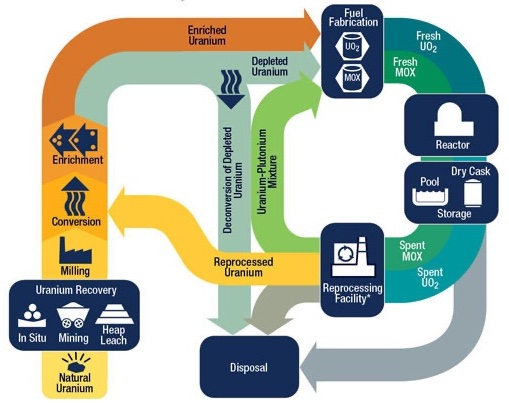
\includegraphics[width=0.8\textwidth]{./Figures/NRCFuelCycle.jpg}
\caption{Illustration of the nuclear fuel cycle (US Nuclear Regulatory Commission)}
\label{Fig:kinetics_nuclearFuelCycle}
\end{center}
\end{figure}

Before going into the analysis of the reactor, it is helpful to zoom out to the big picture of how the entire nuclear fuel cycle functions. This is depicted in Fig.~\ref{Fig:kinetics_nuclearFuelCycle}.

Before going into details, there are two primary types of fuel cycles in use. The US uses a once-through fuel cycle where fuel is put into a reactor, burned, and then disposed of as waste. France and Japan, on the other hand, perform fuel recycling, extracting the plutonium and blending it with uranium fuel to make mixed-oxide or MOX fuel assemblies that are then put back into reactors for additional burnup. 

The advantages of recycling is that it has a greater resource utilization and reduces the quantity of spent nuclear fuel that must be managed. The disadvantage is this comes at an increased cost, as mining uranium is inexpensive. Second, there is an increased risk of diversion of weapons usable materials. While reactor grade plutonium contains too much $^{240}$Pu to be an ideal nuclear explosive and is not the most attractive route for a nation state to pursue, it is nonetheless possible to use it for that purpose. This increased risk must be offset by increased costs to minimize the possibilities of such fuel diversions.

The once-through nuclear fuel cycle consists of the following major steps:
\begin{enumerate}
  \item Mining -- uranium is obtained by extracting it from ores underground resources. Like all mining, this is a polluting industry and is arguably the most environmentally damaging part of the nuclear fuel cycle. The argument in favor is because of the energy density of nuclear fuels, we require less mining than other energy sources.
  \item Milling -- the raw uranium ore must be extracted and comes in the composition of U$_3$O$_8$, which is sometimes called yellowcake. 
  \item Conversion -- in the US, fuel must be enriched and U$_3$O$_8$ is not a chemical form that permits this. We convert it into UF$_6$, which readily enters a gaseous phase.
  \item Enrichment -- the gaseous UF$_6$ is put into fast moving centrifuges. Because of the small mass differential between $^{235}$U and $^{238}$ the centrifugal forces preferentially push one isotope out more than other. The stock is moved through a series of such centrifuges until a desired enrichment (usually a few percent) is reached.
  \item Fuel Fabrication -- the enriched UF$_6$ is converted into ceramic UO$_2$ and sintered into pellets and sealed into fuel cladding tubes. These fuel rods are then put into bundles or assembles that are delivered to a power plant.
  \item Reactor -- the fuel is put into the reactor and is used to cause fission, producing thermal and then electrical energy. A typical fuel assembly resides in the reactor between 3-6 years.
  \item Onsite Storage -- once the fuel is sufficiently depleted it is moved out of the reactor for storage. Because of the large inventory of fission products, the fuel continues to generate a large amount of heat because of radioactive decay that must be removed. This is done by placing them into a spent fuel pool where the fuel assembly resides for several years. Once the radioactive inventory has decreased enough, the fuel is moved out of the pool and placed in dry casks that are cooled with air.
  \item Long-term Repository -- while not yet in operation, the plan in the US is to move the fuel in the spent fuel casks into a long-term or permanent repository for final disposition.
\end{enumerate}
 
In a fuel-recycle scenario, sometime after the fuel is removed from the reactor, it is sent to a reprocessing facility where it is chemically dissolved and separated. The plutonium is extracted and then mixed with uranium to create fuel with enough reactivity to go back into a reactor. The recycling process produces waste that must similarly be disposed of, but the volume and radiotoxicity is much less. 

More advanced fuel cycles are currently being investigated that make use of fast reactors that are capable of burning up the fissionable (but not fissile) actinides with long half lives that account for much of the radiotoxicity on the 1,000 to 100,000 year timeframe. While the technology is theoretically in place, it has yet to be demonstrated in an economically competitive manner.

\subsection{Fuel Burnup}

Zooming back into the reactor eventually, the fuel becomes too depleted to effectively sustain a chain reaction and must be removed from the reactor. This can be mitigated by reshuffling the fuel and mixing it with fresh fuel assemblies, but there are still limits. The limiting factor is not the availability of fuel per se, but rather the fuel experiences steady damage from the energetic fission fragments. Additionally, the buildup of these fragments changes the chemistry, leading to corrosive chemical interactions with the cladding. Also, some of the fission products are gases and these fill the sealed fuel-cladding tube and lead to an increase in internal pressure. As the fuel continues to burn up, its structural integrity diminishes and the probability of fuel failure increases with time. Therefore, fuel inventory concerns aside, it is necessary to remove the fuel from the reactor after a few years lest the fuel rods begin to fail and leak fission products into the coolant.

We quantify the fuel exposure to neutrons with a quantity called \emph{burnup}, which is defined as
\begin{align}
  B = \frac{\text{energy released from fission}}{\text{mass of the fissionable material}} .
\end{align}
Typically we express the energy in units of GWd (GigaWatt days), based on the thermal (not electrical) power of the reactor, and the units of mass as MTU, metric tons of uranium (excluding the mass of oxygen in the conventional UO$_2$ fuel). If different fissionable materials are used, then the mass needs to adjusted accordingly and sometimes the denominator is quoted as mass of heavy metal. Further, the mass of fissionable material typically includes all isotopes, not just, for example, the fissile $^{235}$U.

Typical end-of-life burnups for conventional UO$_2$ fuel is between 30 to 40 GWd/MTU. In recent years, there has been considerable effort to developing fuel capable of handling higher burnup, up to around 60 GWd/MTU, which means they can stay in the reactor longer and more energy can be extracted per unit mass. Advanced reactors such as gas-cooled variants use spherical TRISO fuel kernels that are capable of even higher fuel burnups.

\subsection{Conversion Ratio}

As mentioned, some of the fertile $^{238}$U in a reactor is converted into fissile plutonium isotopes. In a conventional reactor, the depletion of $^{235}$U cannot keep up with the creation of plutonium. However, it is possible to create more fuel than is burned in a \emph{breeder reactor}. For thermal reactors, we use a thorium-based cycle where the fertile $^{232}$Th captures neutrons and produces (after a couple $\beta^-$ decays) fissile $^{233}$U, which is the actual fuel. In fast reactors, we typically convert $^{238}$U into Pu isotopes in an external blanket that can then be extracted, chemically separated, and used to make more fuel for other reactors. In the early days of nuclear power, the known resources of uranium was thought to be much more limited than it actually is. Today, there is a large supply of economically mineable uranium resources such that the resource question is far less of an short or medium term concern. That said, there is still interest in thorium cycles or fast reactors, but these are driven by other factors rather than long-term uranium resources.

Regardless of whether the intent is to breed new fuel, some will be produced and this quantity is called the \emph{conversion ratio}. This is
\begin{align}
  C = \frac{\text{production rate of fissile atoms}}{\text{consumption rate of fissile atoms}} .
\end{align}
In a conventional reactor, the conversion ratio is less than one, i.e., the fuel is burned faster than it is produced. For a typical thermal power reactor, this conversion ratio is on the order of 0.5 to 0.6. In a breeder reactor, the conversion ratio is greater than one and is then usually called the \emph{breeding ratio}.

\subsection{Fuel Depletion Equations} \label{Sec:kinetics_fuelDepletionEquations}

Analyzing the depletion of the reactor is actually a very complicated process. Modern methods typically consider every reaction pathway and fission product individually, considering their radioactive decay. This is done by solving the rate equations including depletion and production, which is a series of first-order ordinary differential equations in each spatial region that depends on the local scalar flux $\phi(\pos,t)$. 

The general form of a rate equation in a reactor for isotope $i$ with concentration $N_i$ is
\begin{align}
  \frac{dN_i}{dt} &= 
  \underbrace{\sum_j \lambda_{ji} N_j(t) }_{\parbox{2.25cm}{\scriptsize rate isotope $i$ is produced from radioactive decay of all isotopes $j$}}
  + \underbrace{\sum_j \gamma_{ji} \sigma_{f,j} \phi(t) N_j(t)}_{\parbox{3.5cm}{\scriptsize rate isotope $i$ is produced from fission from all fissionable isotopes $j$}}
  + \underbrace{\sum_j \sigma_{ji} \phi(t) N_j(t)}_{\parbox{2.75cm}{\scriptsize rate isotope $i$ is produced from all non-fission nuclear reactions with isotopes $j$}} \nonumber \\
  &- \underbrace{\sum_x \sigma_{x,i} \phi(t) N_i(t)}_{\parbox{3cm}{\scriptsize rate isotope $i$ is removed because of all nuclear reactions $x$}}
  - \underbrace{\lambda_i N_i(t) }_{\parbox{1.75cm}{\scriptsize rate isotope $i$ is removed by radioactive decay}}.
\end{align}
Here
\begin{align}
  \lambda_{ji} &= \text{decay constant for isotope $j$ decaying to isotope $i$},  \nonumber \\
  \gamma_{ji}  &= \text{fission product yield for isotope $i$ from fissionable nucleus $j$}, \nonumber \\
  \sigma_{ji}  &= \text{reaction cross section for conversion from isotope $j$ into $i$}, \nonumber \\
  \sigma_{x,i} &= \text{cross section for reaction $x$ of isotope $i$}, \nonumber \\
  \lambda_i    &= \text{decay constant for isotope $i$ (for all decays)}. \nonumber 
\end{align}
An equation is written down for each isotope $i$. These equations can then be formed into a linear system as
\begin{align}
  \frac{d\mathbf{N}}{dt} = \mathbf{A}(t) \mathbf{N}(t) ,
\end{align}
where the coefficient matrix $\mathbf{A}$ depends on both the nuclear data and the local scalar flux $\phi(t)$, which carries the time dependence of the matrix. 

If we assume that the scalar flux is constant over some time interval, i.e., a time step in a calculation $t_i \le t < t_{i+1}$, then this system has a solution as the matrix exponential,
\begin{align}
  \mathbf{N}(t) = \exp\left[ (t-t_i) \mathbf{A} \right] \mathbf{N}(t_i) , \quad t_i \le t < t_{i+1} ,
\end{align}
where $\mathbf{N}(t_i)$ is a known initial condition at $t = t_i$, the beginning of the interval.

The complication that arises is similar to that of the fission product poisons in that the changes in local isotopics leads to a change in the local flux. This means that the depletion equations are non-linear and need to be solved numerically on a time grid that is fine enough to capture the temporal changes of the isotopic concentrations. 

The typical numerical scheme used is called the \emph{predictor-corrector method}. The idea is to break the reactor fueling cycle into a series of time steps that are sufficiently small to capture any changes in the reactor conditions. Typically, this means we need a relatively short time step or two to account for the buildup to the equilibrium states of the fission product poisons $^{135}$Xe and $^{149}$Sm every time the reactor changes its power level. Then, we need to take time steps of on the order of a few weeks to capture slower, long term fuel depletion and fertile conversion effects.

Suppose the isotopic compositions are known at the beginning of time step $t_i$ and given in a vector $\mathbf{N}(t_i)$ . We can then solve the neutron transport or diffusion equations using these componsitions with some numerical scheme to get the consistent scalar fluxes. We call these $\phi_1(t_i)$.

We then plug the scalar flux $\phi_1(t_i)$ into the system of rate equations and solve them at each position in the reactor to arrive at a \emph{prediction} of the new isotopic composition vector $\hat{\mathbf{N}}(t_i)$. We could use this prediction as the new isotopic compositions $\mathbf{N}(t_{i+1})$, but it turns out doing this, wile simple, would require taking very large time steps.

Instead, we use this new vector as input into the neutron transport and diffusion equation and solve for an updated scalar flux using the new compositions that we call $\phi_2(\pos,t_i)$. We then go back and compute a \emph{corrected} isotopic composition by using the average of the scalar fluxes,
\begin{align}
  \phi(t_i) = \frac{ \phi_1(t_i) + \phi_2(t_i) }{ 2 } ,
\end{align}
as the scalar flux to compute $\mathbf{N}(t_{i+1})$. We then use this as the initial condition of for the next time step. Because the core composition has changed, we then need to perform a criticality search after each time step based on changing control rod heights or soluble boron concentrations.

Note again that these equations must be solved for all locations in the reactor, so it can become a rather computationally taxing task for a large reactor with numerous fuel pins. Using the predictor-corrector method significantly improves the accuracy of the depletion solve over forward Euler and allows for taking much larger time steps than would be possible otherwise. More sophisticated methods exist, and finding better depletion solver techniques that balance accuracy versus computational costs remains an open area of study.

One thing worth mentioning is that the coefficients in the matrix $\mathbf{A}$ span several orders of magnitude. This implies we have phenomena that occur on timescales ranging from milliseconds to millions of years. It turns out that evaluating the matrix exponential is actually difficult in this case because of numerical precision issues. While this problem has not completely gone away, the last few decades have seen advances in numerical solution techniques capable of handing what we term stiff systems of differential equations, and the issue is far less acute than it used to be.

\subsection{Estimation of Fuel Cycle Length}

The depletion equations can be solved using numerical schemes to determine the fuel cycle length. Normally, the cycle ends when the fuel inventory has been depleted to the point where there is no remaining excess reactivity to make the reactor critical.

We can perform a simple analysis assuming a one-speed, infinite homogeneous medium to illustrate the general considerations, even though such a model is mostly of pedagogical use. We assume that the reactor is operated at a constant power (not a constant flux), which implies that
\begin{align}
  \Sigma_a^F(t) \phi(t) = \Sigma_a^F(0) \phi(0) , \label{Eq:kinetics_simplifiedBurnup_constantPowerFuelXS}
\end{align}
where $\Sigma_a^F(0)$ is the initial fuel loading and $\phi(0)$ is the initial flux level. This implies that the flux must change in time, specifically increasing to offset fuel depletion.

To solve for $\phi(t)$, we write s simple rate equation for the depletion of the fuel,
\begin{align}
  \frac{dN^F}{dt} = -\sigma_a^F N^F(t) \phi(t) = -\sigma_a^F N^F(0) \phi(0) .
\end{align}
Here we used the fact that $\Sigma_a^F \phi$ is constant over the cycle. (We also neglect the radioactive decay of the fuel, which, while not strictly true, is a reasonable assumption since the half life of any practical reactor fuel is going to be much greater than the cycle length.) Since the right-hand side is constant, we can simply integrate this to obtain the fuel atomic density as a function of time,
\begin{align}
  N^F(t) = N^F(0) -\sigma_a^F N^F(0) \phi(0) t = N^F(0) \left[ 1 - \sigma_a^F \phi(0) t \right] .
\end{align}
Multiplying the extreme left and right hand side by $\sigma_a^F$, we get the macroscopic fuel cross section as a function of time,
\begin{align}
  \Sigma_a^F(t) = \Sigma_a^F(0) \left[ 1 - \sigma_a^F \phi(0) t \right] . \label{Eq:kinetics_simplifiedBurnup_fuelAbsorptionXS_time}
\end{align}

We then substitute this into Eq.~\eqref{Eq:kinetics_simplifiedBurnup_constantPowerFuelXS} to obtain the relationship
\begin{align}
  \Sigma_a^F(0) \left[ 1 - \sigma_a^F \phi(0) t \right] \phi(t) = \Sigma_a^F(0) \phi(0) . \nonumber
\end{align}
We can then easily solve this for the scalar flux as a function of time,
\begin{align}
  \phi(t) = \frac{\phi(0)}{ 1 - \sigma_a^F \phi(0) t } . \label{Eq:kinetics_simplifiedBurnup_scalarFlux_time}
\end{align}
We refer to this as the flux history of the reactor needed to ensure a constant power.

For a single thermal energy group, we can write the effective multiplication factor $k$ as the product of the thermal fission factor $\eta = \nu\Sigma_f^F/\Sigma_a^F$ and the thermal utilization factor $f = \Sigma_a^F/\Sigma_a$. Here the absorption cross section $\Sigma_a$ includes components from the fuel $\Sigma_a^F$, moderator $\Sigma_a^M$, fission product poisons $\Sigma_a^P$, and control mechanisms $\Sigma_a^P$. Here we neglect the conversion of fertile to fissile isotopes to simplify the analysis. (Again, this is a pedagogical model anyway.) 

The effective multiplication factor is then
\begin{align}
  k = \eta f = \frac{ \eta \Sigma_a^F(t) }{ \Sigma_a^F(t) + \Sigma_a^M + \Sigma_a^P(t) + \Sigma_a^C(t) } = 1.
\end{align}
The control mechanism cross section is the operational parameter that can be adjusted to maintain criticality. We can solve for the control cross section as
\begin{align}
  \Sigma_a^C(t) = ( \eta - 1 ) \Sigma_a^F(t) - \Sigma_a^M - \Sigma_a^P(t) . \label{Eq:kinetics_simplifiedBurnup_controlXS}
\end{align}

Because we assumed no conversion of fertile isotopes, the fuel will deplete with time, decreasing $\Sigma_a^F$. Simultaneously, fission product poisons will build up so $\Sigma_a^P$ increases. These poisons include $^{135}$Xe, $^{149}$Sm, and a lumped permanent fission product poison contribution that does not saturate. Eventually, the amount of control needed to achieve criticality decreases to zero, and this time $t_c$ is the end of the fuel cycle.

What remains is determining how the fission product poisons build up with time. As we said, there are three contributions: xenon, samarium, and other permanent poisons. We write this as
\begin{align}
  \Sigma_a^P(t) = \Sigma_a^X(t) + \Sigma_a^S(t) + \Sigma_a^{fp}(t) .
\end{align}
We assume that both $^{135}$Xe and $^{149}$Sm reach an equilibrium state instantaneously, which is justified by the fuel cycle length being much longer than the buildup of either of those poisons. While the flux is changing continuously as a function of time, which renders the concept of ``equilibrium'' a bit suspect, we note that the flux increases as $(1-at)^{-1}$, which is fairly gradual. Therefore, we can just say the fission product poison precursors $^{135}$I and $^{149}$Pm change slow enough that the poisons themselves maintain a quasi-equilibrium.

The $^{135}$Xe cross section can be obtained by multiplying Eq.~\eqref{Eq:kinetics_xenonEquilibrium} by the $^{135}$Xe capture cross section $\sigma_a^X$ to obtain
\begin{align}
  \Sigma_a^X(t) = \frac{ ( \gamma_I + \gamma_X ) \Sigma_f(t) \phi(t) }{ \lambda_X / \sigma_a^X + \phi(t) } = \frac{ ( \gamma_I + \gamma_X ) \Sigma_f(0) \phi(0) }{ \lambda_X / \sigma_a^X + \phi(t) } .
\end{align}
Here we used the fact that we are keeping the power constant. For samarium, we get
\begin{align}
  \Sigma_a^S(t) = \gamma_P \Sigma_f(t) .
\end{align}

Next, we have to handle the permanent fission product poisons. These build up continuously and we assume that any when any poison captures a neutron it converts into an equivalent poison isotope. This is described by the rate equation,
\begin{align}
  \frac{dN^{fp}}{dt} = \gamma_{fp} \Sigma_f(t) \phi(t) = \gamma_{fp} \Sigma_f(0) \phi(0) , \quad N^{fp}(0) = 0.
\end{align}
Here again, the power is assumed to be constant so the right-hand side is a constant. We also assume there is initially no fission product poison, which is the case for fresh fuel. We can easily integrate this and multiply by the absorption cross section for the permanent fission product poison $\sigma_a^{fp}$ to obtain
\begin{align}
  \Sigma_a^{fp}(t) = \gamma_{fp} \sigma_a^{fp} \Sigma_f(0) \phi(0) t.
\end{align}

Inserting these equations into Eq.~\eqref{Eq:kinetics_simplifiedBurnup_controlXS} for the control cross section we get
\begin{align}
  \Sigma_a^C(t) &= ( \eta - 1 ) \Sigma_a^F(t) - \Sigma_a^M - \frac{ ( \gamma_I + \gamma_X ) \Sigma_f(0) \phi(0) }{ \lambda_X / \sigma_a^X + \phi(t) } \nonumber \\
   &- \gamma_P \Sigma_f(t) - \gamma_{fp}  \sigma_a^{fp} \Sigma_f(0) \phi(0) t .
\end{align}
Now we have a bit of a hybrid notation here, with some terms involving the fission cross section and the others involving the fuel absorption cross section. To clean this up, we convert relate the fission to the absorption cross section. For this we write the capture to fission ratio as,
\begin{align}
  \kappa = \frac{\Sigma_\gamma^F}{\Sigma_f} = \frac{\Sigma_a^F - \Sigma_f}{\Sigma_f} = \frac{\Sigma_a^F}{\Sigma_f} - 1,
\end{align}
which we is constant in time since the nuclear properties do not vary, only the number densities. (One could argue the underlying spectrum to get the one-group cross section changes, but we are neglecting that.) This implies that
\begin{align}
  \Sigma_f(t) = \frac{\Sigma_a^F(t)}{ 1 + \kappa } .
\end{align}

Inserting this into the expression for the control cross section, we have
\begin{align}
    (1 + \kappa) \Sigma_a^C(t) &= ( \eta - 1 ) (1 + \kappa) \Sigma_a^F(t) -  (1 + \kappa) \Sigma_a^M - \frac{ ( \gamma_I + \gamma_X ) \Sigma_a^F(0) \phi(0) }{ \lambda_X / \sigma_a^X + \phi(t) } \nonumber \\
   &- \gamma_P \Sigma_a^F(t) - \gamma_{fp}  \sigma_a^{fp} \Sigma_a^F(0) \phi(0) t .
\end{align}
By Eq.~\eqref{Eq:kinetics_simplifiedBurnup_fuelAbsorptionXS_time}, we can replace $\Sigma_a^F(t)$ and divide by $\Sigma_a^F(0)$ to obtain
\begin{align}
    (1 + \kappa) \frac{\Sigma_a^C(t)}{\Sigma_a^F(0)} &= ( \eta - 1 ) (1 + \kappa)\left[ 1 - \sigma_a^F \phi(0) t \right] -  (1 + \kappa) \frac{\Sigma_a^M}{\Sigma_a^F(0)} \nonumber \\*
    &- \frac{ ( \gamma_I + \gamma_X )  \phi(0) }{ \lambda_X / \sigma_a^X + \phi(t) } 
     - \gamma_P  \left[ 1 - \sigma_a^F \phi(0) t \right] - \gamma_{fp} \sigma_a^{fp} \phi(0) t .
\end{align}

The ratio of the moderator to the initial fuel density can be related to the excess reactivity at the beginning of the fuel cycle. To see this, we write
The excess reactivity is
\begin{align}
  \rho_{ex} = 1 - \frac{1}{k(0)} = 1 - \frac{1}{\eta f(0)} 
  = 1 - \frac{\Sigma_a^F(0) + \Sigma_a^M}{\eta \Sigma_a^F(0)}
  = \frac{ (\eta-1) \Sigma_a^F(0) - \Sigma_a^M}{ \eta \Sigma_a^F(0)} 
\end{align}
This implies
\begin{align}
   \frac{\Sigma_a^M}{\Sigma_a^F(0)} = \eta - 1 - \eta \rho_{ex} .
\end{align}
Therefore,
\begin{align}
    (1 + \kappa) \frac{\Sigma_a^C(t)}{\Sigma_a^F(0)} 
    &= ( \eta - 1 ) (1 + \kappa)\left[ 1 - \sigma_a^F \phi(0) t \right] -  (\eta - 1 )(1 + \kappa) + ( 1 + \kappa ) \eta \rho_{ex} \nonumber \\*
    &- \frac{ ( \gamma_I + \gamma_X )  \phi(0) }{ \lambda_X / \sigma_a^X + \phi(t) } 
     - \gamma_P  \left[ 1 - \sigma_a^F \phi(0) t \right] - \gamma_{fp} \sigma_a^{fp} \phi(0) t \nonumber \\
    &= -( \eta - 1 ) (1 + \kappa)  \sigma_a^F \phi(0) t   + ( 1 + \kappa ) \eta \rho_{ex} \nonumber \\*
    &- \frac{ ( \gamma_I + \gamma_X )  \phi(0) }{ \lambda_X / \sigma_a^X + \phi(t) } 
     - \gamma_P  \left[ 1 - \sigma_a^F \phi(0) t \right] - \gamma_{fp} \sigma_a^{fp} \phi(0) t .
\end{align}

Now we observe for typical power reactors, $\phi(t) \gg \lambda_X / \sigma_a^X$. This allows the denominator of the xenon poison term to simplify. We can then apply Eq.~\eqref{Eq:kinetics_simplifiedBurnup_scalarFlux_time} to put $\phi(t)$ in terms of the initial scalar flux. We obtain
\begin{align}
    (1 + \kappa) \frac{\Sigma_a^C(t)}{\Sigma_a^F(0)} 
    &= -( \eta - 1 ) (1 + \kappa)  \sigma_a^F \phi(0) t   + ( 1 + \kappa ) \eta \rho_{ex} \nonumber \\*
    &- ( \gamma_I + \gamma_X ) \left[ 1 - \sigma_a^F \phi(0) t \right]
     - \gamma_P  \left[ 1 - \sigma_a^F \phi(0) t \right] - \gamma_{fp} \sigma_a^{fp} \phi(0) t .
\end{align}

Finally, we are ready to determine the cycle length. Recall at the end of cycle, the control cross section $\Sigma_c$ goes to zero. After setting the left-hand side to zero, we can solve for the cycle time as
\begin{align}
  t_c = \frac{ ( 1 + \kappa ) \eta \rho_{ex} - ( \gamma_I + \gamma_X + \gamma_P ) }
  { \left[ ( \eta - 1 ) (1 + \kappa)  \sigma_a^F -  ( \gamma_I + \gamma_X + \gamma_P ) \sigma_a^F + \gamma_{fp} \sigma_a^{fp} \right] \phi(0) } .
\end{align}
The numerator involves both positive and negative terms. This implies to have a positive cycle time, i.e., the reactor can go critical in the first place, we demand the numerator be positive. This puts a lower bound on the excess reactivity of
\begin{align}
  \rho_{ex} > \frac{ \gamma_I + \gamma_X + \gamma_P }{ \eta ( 1 + \kappa ) } = \frac{ \gamma_I + \gamma_X + \gamma_P }{ \nu } .
\end{align}
From this, we see the intuitive results. First, the higher the excess reactivity, the longer the cycle. Second, the higher the initial scalar flux (which then must increase in time to maintain constant power), the shorter the fuel cycle.

\subsection{Fuel Reload Fraction}

A typical power reactor fuel cycle lasts between 18 and 24 months. After this time, the fissile inventory is too low to sustain a chain reaction and new fuel needs to be added. It is not necessary to replace all of the fuel, and it is economically advantageous to minimize the amount of fresh fuel in the next cycle to maximize the utilization of each individual assembly. As such, we typically only replace a fraction of the fuel where a typical assembly will be in the reactor for two or three cycles before reaching its burnup limits where fuel failure becomes a significant concern.

The first task is to determine the reload fraction, which is the fraction of fresh fuel put into the reactor. To begin this analysis, we index each fuel batch $n$ and define $k_n$ as the infinite multiplication for the $n$th batch. For simplicity each batch is assumed to have the same number of fuel assemblies. The overall infinite multiplication factor for $N$ batches in the reactor is then approximately the mean of the infinite multiplication factors for each batch,
\begin{align}
  k = \frac{1}{N} \sum_{n=1}^N k_n .
\end{align}
In reality there is a spatial dependence that needs to be considered for how the assemblies within each batch are laid out (more on this later), but in practice this model works quite well since we strive for a spatially uniform flux distribution during reload by intelligently arranging the fuel and control materials.

The effective multiplication factor for each batch can then be parameterized by the burnup $B$ using a simple linear model:
\begin{align}
  k_n = k_0 - a B_n .
\end{align}
Here $k_0$ is the infinite multiplication factor for fresh fuel and $a$ is some rate coefficient proportional to the power. This linear model works quite well for low-enriched uranium fuel. One weakness is that it does not work particularly well for natural uranium fueled reactors.

We next denote $k_e$ as the end-of-cycle effective multiplication factor. Therefore, the burnup achievable for a reactor cycle consisting of fresh fuel is
\begin{align}
  B_1 = \frac{k_0 - k_e}{a} . \label{Eq:kinetics_fuelReload_burnupSingleCycle}
\end{align}

As mentioned, we do not replace all of the fuel, as it would be inefficient to do so. We can easily calculate the increased utilization of the fuel for a two-cycle case where we replace half of the fuel. The end-of-cycle multiplication factor (after the second pass) is then
\begin{align}
  k_e = \frac{k_0 - a B_2 }{ 2 } + \frac{ k_0 - 2 a B_2 }{ 2 } = k_0 - \frac{3}{2} a B_2 .
\end{align}
The first term is for the new batch and the second term is for the old batch that has now experienced twice the amount of burnup (note the factor of two in the numerator). Here $B_2$ is the burnup after each cycle for the two-fuel batch case. Solving for $B_2$ and using Eq.~\eqref{Eq:kinetics_fuelReload_burnupSingleCycle}, we obtain the relationship between the cycle burnup $B_2$ versus the single cycle $B_1$,
\begin{align}
  B_2 = \frac{2}{3} \frac{k_0 - k_e}{a} = \frac{2}{3} B_1 .
\end{align}
Since each fuel batch goes through two cycles, we multiply this new cycle burnup by a factor of two to get the total burnup as
\begin{align}
  B^{(2)} = 2 B_2 = \frac{4}{3} B_1 .
\end{align}
Here we denote the superscript in parentheses as as the discharge burnup after some number of cycles. Since
\begin{align}
  B^{(1)} = B_1,
\end{align}
we see that a two-cycle refueling with half of the fuel replaced yields one-third more burnup than is possible for a single cycle.

We can extend this to $N$ refueling cycles. Let $B_N$ be the burnup each cycle where the fuel sits in the reactor for $N$ cycles, having a discharge burnup of $B^{(N)}$. The effective multiplication for a fuel batch at the end of the cycle is
\begin{align}
  k_e = k_0 - \frac{1}{N} \sum_{n=1}^N n a B_N . \label{Eq:kinetics_EOCmultiplication_NCycle_Sum}
\end{align}
Using the summation identity
\begin{align}
  \sum_{n=1}^N n = \frac{N(N+1)}{2}, \nonumber
\end{align}
we obtain
\begin{align}
  k_e = k_0 - \left( \frac{N+1}{2} \right) a B_N .  \label{Eq:kinetics_EOCmultiplication_NCycle}
\end{align}
The cyclewise burnup is then
\begin{align}
  B_N = \frac{ 2 ( k_0 - k_e ) }{ a (N+1) } . \label{Eq:kinetics_cycleBurnup_NCycle}
\end{align}
We can then compute the discharge burnup for $N$ cycles as
\begin{align}
  B^{(N)} = N B_N = \frac{ 2 N }{ N + 1 } \left( \frac{ k_0 - k_e }{ a } \right) = \frac{ 2 N }{ N + 1 } B_1.
\end{align}

The limiting case for continuous refueling as $N \rightarrow \infty$ gives a discharge burnup of
\begin{align}
  B^{(\infty)} = 2 B_1 .
\end{align}
This means if we are inserting and removing new fuel continuously as in a molten salt reactor or approximately as a CANDU reactor, we can get twice the burnup per unit of fuel.

\subsection{Initial Excess Reactivity Requirement}

By using multiple refueling batches, we can reduce the amount of excess reactivity needed initially in the reactor. We define $k_{ex}^{(N)}$ as the initial multiplication factor with all control elements removed for an $N$-cycle refueling scheme. At equilibrium we insert the same amount of excess reactivity at the start of each fuel cycle. 

For a single cycle where the core is reloaded with fresh fuel, this is the value $^{(1)} = k_0$. For an $N$-cycle refueling strategy, we have
\begin{align}
  k_{ex}^{(N)} = k_0 - \frac{1}{N} \sum_{n=0}^{N-1} n a B_N = k_0 - \frac{ N - 1 }{ 2 } a B_N .
\end{align}
Here we note the summation index is shifted down by one in contrast to Eq.~\eqref{Eq:kinetics_EOCmultiplication_NCycle_Sum} because this is that the \emph{beginning} of the cycle versus the end. Subtracting Eq.~\eqref{Eq:kinetics_EOCmultiplication_NCycle} from this result yields
\begin{align}
  k_{ex}^{(N)} - k_e = \left( \frac{ N + 1 }{ 2 } \right) a B_N  - \left( \frac{N-1}{2} \right) a B_N = a B_N .
\end{align}
Finally, using Eq.~\eqref{Eq:kinetics_cycleBurnup_NCycle} to eliminate the per cycle burnup $B_N$ we obtain the ratio of the change in the multiplication factor for $N$-cycle to the single cycle:
\begin{align}
  \frac{ k_{ex}^{(N)} - k_e }{ k_0 - k_e } = \frac{2}{N+1} .
\end{align}

Evidently, the amount of excess reactivity needed per cycle is inversely proportional to the number of cycles that fuel is within the reactor. Intuitively, if we continuously refuel we do not require any excess reactivity as we are always able to add more fuel to immediately compensate for the natural loss of reactivity.

\subsection{Spatial Fuel Loading}

The previous analysis make gross simplifications and essentially assumes that we can somehow homogeneously mix the new and old fuel batches. The reality is that a the fundamental unit in a light-water reactor is a fuel assembly and there are often a few hundred of these in a typical reactor core. Each fuel assembly experiences a different local flux history and burnup characteristics depending on the layout and actions taken during operation (e.g., local control rod adjustments). 

The goal of a reactor designer is to select the optimal set and arrangement of fuel assemblies following a reload. Here optimal satisfies several requirements of giving a flat power distribution and maximizing the energy output of each fuel assembly while considering the various operational actions taken in the subsequent fuel cycles.

The number of possible fuel loading combinations scales as the factorial of the number of elements. Therefore, it is impossible to carry out an exhaustive analysis of every scenario. Furthermore, the time available during a refueling to actually perform the calculations and reach a decision is quite limited, being a few weeks for a typical reactor outage, during which the power plant is not generating electricity and not making money. 

Since time is of the essence, we have to settle for a simpler analysis. Typically fuel burnup limitations mean that a fuel assembly goes through two or three fuel loadings before being removed from the reactor. To achieve a flat power distribution, we often put the fresh fuel near the edge of the core. This makes sense since leakage would naturally cause the flux to be lower near the periphery, so we can offset this by surrounding the reactor core with fresh fuel. 

The interior consists of two regions, each containing fuel assemblies that have gone through one or two cycles. Typically we arrange these two zones in a checkerboard fashion putting the higher burnup (and less reactive) assemblies next to those with lower burnup and higher reactivity. Sometimes we put the highest burnup fuel in the center region where leakage effects are the lowest. We would then execute and algorithm that would search over a series of plausible fuel loadings within each group to achieve the desired operational characteristics.

\subsection{Spent Nuclear Fuel}

Fresh fuel in a typical light-water reactor is a few percent enriched, typically containing 3-5\%~$^{235}$U with the vast remainder being $^{238}$U with a very small amount of $^{234}$U. To increase economic competitiveness, commercial nuclear power plants are looking to increase the enrichment into the 5-10\% range, with advanced reactors going just below 20\%, which denotes the line between low and high-enriched uranium. It is certainly advantageous to use highly enriched fuel, and the reasons are not purely technical or even economic, but driven by nuclear nonproliferation concerns. Uranium enriched by 20\% and above could theoretically be used to manufacture a nuclear explosive, even though typical feedstocks for that purpose are in excess of 90\%.

After typical light-water reactor fuel with a few percent enrichment is put into the reactor, the $^{235}$U begins to deplete, either undergoing fission or being captured into not particularly fissionable $^{236}$U. 

The $^{238}$U undergoes either fission from fast neutrons, but mostly gets converted to $^{239}$U via neutron capture, which quickly decays to $^{239}$Np, and then again to fissile $^{239}$Pu. From here $^{239}$Pu can either undergo fission or neutron capture. The capture of neutrons results in $^{240}$Pu, which is a fissionable nuclide with a high capture cross section and a low fission cross section. $^{240}$Pu readily captures neutrons to make $^{241}$Pu, which can either capture neutrons to make $^{242}$Pu or decay to $^{241}$Am. The $^{242}$Pu decays to $^{243}$Pu, which quickly decays to $^{243}$Am. The neutron capture process continues to make other actinides in small quantities. We generally group isotopes that are not the abundant isotopes of uranium and plutonium produced in the nuclear fuel cycle as the \emph{minor actinides}. (There is a bit of ambiguity on which isotopes are precisely minor actinides, with $^{237}$Np being a one in particular, as there is enough of it to produce macroscopic, kilogram quantities.)

The isotope $^{239}$Pu is an excellent fuel for nuclear explosives, and is the major proliferation concern in the nuclear fuel cycle. Thankfully, as $^{239}$Pu builds up, not particularly fissionable $^{240}$Pu is created as well, which limits its utility as a weapons feedstock, even though it is theoretically possible to manufacture a nuclear explosive using any composition of plutonium. Reactors specifically designed to produce plutonium for weapons use short fuel cycles to not give $^{240}$Pu time to build up to a large percentage. Fuel in a commercial reactor is in much longer, typically 3-6 years, which means there is a much higher concentration of $^{240}$Pu, typically on the order of 80\%.

After going through a reactor, the material is referred to as spent nuclear fuel. The fissionable inventory consists of the following constituents with rough percentages:
\begin{enumerate}
  \item Some $^{235}$U remains in the reactor. Typically the enrichment is less than 1\%, and on the order of what is found in natural uranium ore.
  \item Most of the fuel is still $^{238}$U with a composition between 90-95\%, typically closer to the upper ebd of this range.
  \item About 1-2\% of the fuel has been converted into various isotopes of plutonium. About 80-85\% of this is $^{239}$Pu.
  \item A few tenths of a percent are minor actinides, most of which are neptunium, americium, and curium.
  \item The remaining about 5\% of the isotopes are fission products.
\end{enumerate}

This brew of actinides and fission products is the waste stream produced from nuclear power. As mentioned, the plutonium isotopes can be readily used to fabricate mixed-oxide nuclear fuel and reinserted into nuclear reactors. This is not currently done in the US, but it is Japan and France. The minor actinides are a bit more challenging to burn up as many of them are not fissile and therefore do not readily get destroyed in thermal reactors, but could be burned as a fuel in fast reactors.

Initially, most of the radioactivity from spent nuclear fuel is from the stew of fission products. These have a wide range of half lives, from minutes to millions of years. The ones with half lives on the order of minutes, hours, and a few days are particularly important immediately after the reactor shutdown and is of major source of thermal energy release and those with half-lives on the hours to days are a significant radiotoxicity concern during a nuclear accident. $^{131}$I is perhaps the most important of these, produced in great abundance from fission, having an 8-day half life, and being readily taken up biologically into the thyroid, it poses a major health concern in the days and weeks following a large radioactive release. (This fission product is the reason potassium iodide tablets would be distributed following nuclear accidents or the detonation of a nuclear explosive. The iodine in the tablet saturates the thyroid and prevents the uptake of radioactive $^{131}$I.)

After the spent nuclear fuel has cooled for months or a few years, all the short-lived fission products have decayed. The two fission product isotopes that contribute a large radiological hazard on this time scale are $^{90}$Sr and $^{137}$Cs with a half lives of 28 and 30 years respectively. These take a few hundred years to decay away. After about 250-300 years, the radiotoxicity from fission products has fission products has diminished significantly. There are a handful of fission products with very long half-lives, with $^{99}$Tc (211,000 year half life) being most responsible for the radioactivity of the long-lived fission products.

\begin{figure}[tb!]
\begin{center}
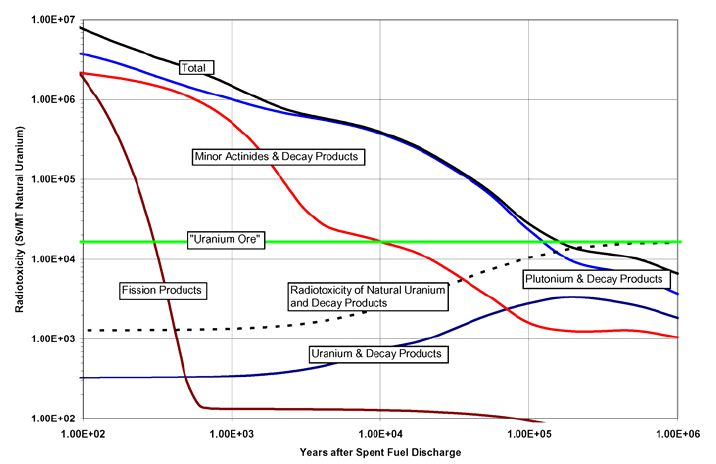
\includegraphics[width=1.0\textwidth]{./Figures/NEASpentNuclearlFuel.jpeg}
\caption{Radiotoxicity of Spent Nuclear Fuel by Component (NEA report 6090, 2006)}
\label{Fig:kinetics_spentNuclearFuelRadiotoxicity}
\end{center}
\end{figure}

The specific activity of spent nuclear fuel broken down by component is given in Fig.~\ref{Fig:kinetics_spentNuclearFuelRadiotoxicity}. Much of the long-lived radioactivity that is of major concern for the long-term disposal of spent nuclear fuel are the actinides, many of which have half-lives on the order of several thousands or a few tens of thousands of years. It is this range which is most problematic. While less radioactive than the shorter lived fission products, they are still short enough and in large enough quantities to cause a large radiation dose to anyone exposed to the material for tens of thousands of years. The plutonium isotopes and its decay products would take about 100,000 years to decay to the radioactivity level of natural uranium ore. The minor actinides are a bit shorter and require several thousands of years to similarly decay.

This length of time is much longer than human civilization and therefore plutonium and the minor actinides are the major concern with the long-term disposal of spent nuclear fuel. The fission products alone are a concern, but these \emph{only} need to be isolated for a few hundred years. While this is indeed a very long time, spanning several human lifespans, there is little question about the technical ability to engineer containers able to endure for this length of time. Indeed this provides the major motivation for recycling of spent nuclear fuel, as engineering barriers that hold for tens of thousands of years is highly questionable.

The issue of spent nuclear fuel disposal is both a technical challenge in addition to difficult raising questions of policy and environmental justice. Entire books have been written on this topic, and we will not attempt to address those questions here other than to note that radioactive wastes have a finite lifetime, as they are continually becoming less toxic overall as the natural process of radioactive decay proceeds. Other industrial wastes, produced in far greater quantities, have effectively infinite lifetimes. So while the disposal of spent nuclear fuel is an important societal problem that needs to be addressed, other than its toxicity being derived from radiation as opposed to chemistry, the questions it poses are very similar. Indeed, because of the energy density of nuclear fuels, the quantities generated are much smaller and are quite manageable.





\end{document}
